%%%%%%%%%%%%%%%%%%%%%%%%%%%%%%%%%%%%%%%%%%%%%%%%%%%%%%%%%%%%%%%%%%%%%%%%%%
%
% Generic template for TFC/TFM/TFG/Tesis at UAH
%
% $Id: book.tex,v 1.24 2019/11/29 09:31:24 macias Exp $
%
% By:
%  + Javier Macías-Guarasa.
%    Departamento de Electrónica
%    Universidad de Alcalá
%  + Roberto Barra-Chicote.
%    Departamento de Ingeniería Electrónica
%    Universidad Politécnica de Madrid
%
% Based on original sources by Roberto Barra, Manuel Ocaña, Jesús Nuevo,
% Pedro Revenga, Fernando Herránz and Noelia Hernández. Thanks a lot to
% all of them, and to the many anonymous contributors found (thanks to
% google) that provided help in setting all this up.
%
% See also the additionalContributors.txt file to check the name of
% additional contributors to this work.
%
% If you think you can add pieces of relevant/useful examples,
% improvements, please contact us at (macias@depeca.uah.es)
%
% You can freely use this template and please contribute with
% comments or suggestions!!!
%
%%%%%%%%%%%%%%%%%%%%%%%%%%%%%%%%%%%%%%%%%%%%%%%%%%%%%%%%%%%%%%%%%%%%%%%%%%%

% This is for rubber to clean additional files (do not remove!!)
% rubber: clean book.acn book.acr book.alg book.cod book.ist book.out book.sbl book.slg book.sym book.lor book.glsdefs book.loa
% rubber: onchange book.glo 'makeglossaries book'
% rubber: watch book.glo book.acr book.sym book.slg book.alg

\documentclass[english,openright]{book}

%%%%%%%%%%%%%%%%%%%%%%%%%%%%%%%%%%%%%%%%%%%%%%%%%%%%%%%%%%%%%%%%%%%%%%%%%%%
% BEGIN Preamble and configuration section
%
%%%%%%%%%%%%%%%%%%%%%%%%%%%%%%%%%%%%%%%%%%%%%%%%%%%%%%%%%%%%%%%%%%%%%%%%%%% 
% 
% Generic template for TFC/TFM/TFG/Tesis
% 
% $Id: preamble.tex,v 1.34 2017/04/06 13:56:12 macias Exp $
% 
% By:
% + Javier Macías-Guarasa. 
%   Departamento de Electrónica
%   Universidad de Alcalá
% + Roberto Barra-Chicote. 
%   Departamento de Ingeniería Electrónica
%   Universidad Politécnica de Madrid   
% 
% Based on original sources by Roberto Barra, Manuel Ocaña, Jesús Nuevo,
% Pedro Revenga, Fernando Herránz and Noelia Hernández. Thanks a lot to
% all of them, and to the many anonymous contributors found (thanks to
% google) that provided help in setting all this up.
% 
% See also the additionalContributors.txt file to check the name of
% additional contributors to this work.
% 
% If you think you can add pieces of relevant/useful examples,
% improvements, please contact us at (macias@depeca.uah.es)
% 
% You can freely use this template and please contribute with
% comments or suggestions!!!
% 
%%%%%%%%%%%%%%%%%%%%%%%%%%%%%%%%%%%%%%%%%%%%%%%%%%%%%%%%%%%%%%%%%%%%%%%%%%% 

%% FIXING PROBLEM WITH ALL PAGES PRINTED IN COLOR \documentclass[RGB,rgb,svgnames,spanish,openright]{book}
%\documentclass[spanish,openright]{book}
% \documentclass[english,openright]{book}
% \documentclass[11pt,english,twoside,openright]{book}

% \usepackage[a4,cam,center]{crop}
% \crop[font=\upshape\mdseries\small\textsf]

\synctex=1

% To generate a proper PDF/A document
%\usepackage[a-1b]{pdfx}

% To allow changing the default alignment of an image
\usepackage[export]{adjustbox}

% To allow simple notes to be used in the review process (see defined
% commands at the end of this file)
\usepackage{todonotes} 

% ifthen to allow using language dependent settings
\usepackage{ifthen}

%% JMG: FIXING PROBLEM WITH ALL PAGES PRINTED IN COLOR
% This should not be touched, as it should work as it is know.
\newcommand{\colorspaceused}{rgb}

%The next section seems to be useless, but it's still pending to try further
\ifthenelse{\equal{\colorspaceused}{rgb}}
{
  \PassOptionsToPackage{rgb}{xcolor}% NB: put this *before* \usepackage{pst-all}
}
{
  \PassOptionsToPackage{cmyk}{xcolor}% NB: put this *before* \usepackage{pst-all}
}

\usepackage{iftex}
%\usepackage[latin1]{inputenc} % Para poder escribir con acentos y ñ. en
                              % latin1
\ifPDFTeX
  \usepackage[utf8]{inputenc} % Para poder escribir con acentos y ñ.
  \usepackage[T1]{fontenc}      % Para que haga bien la ``hyphenation''. No
\fi                                % usar si no es necesario, porque ralentiza muchisimo la compilación.
\usepackage{ae}               % Para que todas las fuentes sean Type1, y ninguna Type3.
\usepackage{lmodern}          % This generates a pdf with searchable
                              % accented characters!!!!!!!!!!!!!!!!!!!!!!!!!!!!!!!!!!!!!!!


\usepackage{wrapfig}
\usepackage{lipsum}

% Use this if you want to include pdf files in the final document
\usepackage[final]{pdfpages}

% Use this if you want to delete headers and footers in empty pages
\usepackage{emptypage}

% \usepackage[nottoc]{tocbibind}
\usepackage{tocbibind}

\usepackage{listings}
\usepackage{longtable}
\usepackage{afterpage}

\usepackage{xspace}
\usepackage{verbatim}
\usepackage{moreverb}
\usepackage{multicol}
\usepackage{amsmath}
\usepackage{eurosym}
%\usepackage{subfig} % subfigure is obsolete... 
\usepackage{multirow}
\usepackage{fancyhdr}
\usepackage{makeidx}
\usepackage{rotating}
\usepackage{supertabular}
\usepackage{hhline}
\usepackage{array}
\usepackage[automake,acronym,shortcuts,nomain,hyperfirst=false]{glossaries}
\usepackage{booktabs}
\usepackage{adjustbox}
\usepackage{graphicx}
\newcolumntype{P}[1]{>{\centering\arraybackslash}p{#1}}
\usepackage[ruled,vlined]{algorithm2e}
\newcommand{\eg}{\textit{e}.\textit{g}.}
\newcommand{\ie}{\textit{i}.\textit{e}.}
\newcommand{\aka}{\textit{a}.\textit{k}.\textit{a}}
\newcommand{\wrt}{\textit{w}.\textit{r}.\textit{t}}
% \usepackage{algorithm}% http://ctan.org/pkg/algorithms
% \def\eg{\emph{e.g}\onedot} \def\Eg{\emph{E.g}\onedot}
% \def\ie{\emph{i.e}\onedot} \def\Ie{\emph{I.e}\onedot}
% \usepackage{algpseudocode}% http://ctan.org/pkg/algorithmicx
% \usepackage{algorithm}
% \usepackage[noend]{algpseudocode}
\usepackage{siunitx}
\usepackage{makecell}

%% FIXING PROBLEM WITH ALL PAGES PRINTED IN COLOR
% \usepackage{xcolor}
% \usepackage[RGB,rgb]{xcolor}
% \usepackage{color}
% Pantone 160
% \definecolor{headingPortadaTFM}{RGB}{158,84,10}
% Pantone 160C (this is supposed to be the correct one, but it looks horrible in screen)
% \definecolor{headingPortadaTFM}{RGB}{161,86,28}
% Gold in RGB
% \definecolor{textoHeadingPortadaTFM}{RGB}{215,215,0}
% Captured colors in screen (this looks pst on screen)

% \ifthenelse{\equal{\colorspaceused}{rgb}}
% {
%   \definecolor{headingPortadaTFM}{RGB}{152,118,52}
%   \definecolor{textoHeadingPortadaTFM}{RGB}{208,205,102}
% }
% {
%   % These definitions are for cmyk colorspace
%   \definecolor{headingPortadaTFM}{cmyk}{0.0254,0,0.559,0.537}
%   \definecolor{textoHeadingPortadaTFM}{cmyk}{0,0.0144,0.51,0.184}
% }

% http://latexcolor.com/

\definecolor{pantone293}{RGB}{35,91,168}

\definecolor{headingPortadaTFG}{RGB}{152,118,52}
\definecolor{headingPortadaTFM}{RGB}{0,90,170}
\definecolor{textoHeadingPortadaTFM}{RGB}{208,205,102}
\definecolor{textoHeadingPortadaTFG}{RGB}{208,205,102}

\definecolor{gray97}{gray}{.97}
\definecolor{gray75}{gray}{.75}
\definecolor{gray45}{gray}{.45}

\definecolor{ForestGreen}{RGB}{34,139,34}
\definecolor{YellowOrange}{rgb}{1.0, 0.75, 0.0}
\definecolor{aqua}{rgb}{0.0, 1.0, 1.0}

% To draw rectagles in tfm cover
\usepackage{tikz}


% \usepackage[authoryear]{natbib}
% \makeatletter
% \let\NAT@parse\undefined
% \makeatother
% \usepackage{natbib}

\usepackage{geometry}
\geometry{verbose,a4paper,tmargin=2.5cm,bmargin=2.5cm,lmargin=2.5cm,rmargin=2.5cm}
% \geometry{paperwidth=210mm,paperheight=297mm}

%\usepackage[hang, flushmargin]{footmisc}   

\usepackage{hyperxmp}
\usepackage[
%% ps2pdf,                %%% hyper-references for ps2pdf
bookmarks=true,%                   %%% generate bookmarks ...
bookmarksnumbered=true,            %%% ... with numbers
hypertexnames=false,               %%% needed for correct links to
%%% figures!!!
% hypertexnames=true,               %%% needed for correct links on pagebackrefs!!!
breaklinks=true,                   %%% breaks lines, but links are very small
% pagebackref=true,
% linktocpage=true,                 %%% enlace en el numero de página.
linktoc=all,
colorlinks=true,
linkcolor=blue,    
citecolor=green,
urlcolor=blue,                     %%% texto  con color (further
%%% modified in myconfig.tex)
% linkbordercolor={0 0 1},           %%% blue frames around links
pdfborder={0 0 112.0},              %%% border-width of frames 
hyperfootnotes=false
]{hyperref}                        %%% will be multiplied with 0.009 by ps2pdf


% \usepackage[all]{hypcap}
\usepackage[center]{caption}
\usepackage{subcaption}


% Para numerar las \subsubsection
\setcounter{secnumdepth}{5}
% para hacer que las \subsubsection aparezcan en el indice
\setcounter{tocdepth}{5}
% \setcounter{lofdepth}{2}
\setcounter{table}{1}
\setcounter{figure}{1}
\setcounter{secnumdepth}{4}


\setlength{\parskip}{1ex plus 0.5ex minus 0.2ex}


\usepackage{multirow}

\usepackage{setspace}
% \renewcommand{\baselinestretch}{10}
\newcommand{\mycaptiontable}[1]{
  \begin{spacing}{0.6}
    % \vspace{0.5cm}
    \begin{quote}
      % \begin{center}
      {{Table} \thechapter.\arabic{table}: #1}
      % \end{center}
    \end{quote}
    % \vspace{1cm}
  \end{spacing}
  \stepcounter{table}
}

\newcommand{\mycaptionfigure}[1]{
  % \vspace{0.5cm}
  \begin{spacing}{0.6}
    \begin{quote}
      % \begin{center}
      {{Figure} \thechapter.\arabic{figure}: #1}
      % \end{center}
    \end{quote}
    % \vspace{1cm}
  \end{spacing}
  \stepcounter{figure}
}

\usepackage{amsmath}

\usepackage{courier}

% ***************************************************************************
% ***************************************************************************
% ***************************************************************************
\usepackage{multirow}
\usepackage{rotating}
\usepackage{setspace, amssymb, amsmath, epsfig, multirow, colortbl, tabularx}%
% For acronym package:
% If footnote is specified, text will be included in a footnote
% If printonlyused is specified, only used acronyms will be included
% I use the acronym sty under the sty directory as I needed the newest version
% \usepackage[footnote,printonlyused,withpage]{acronym} 
% \usepackage[printonlyused]{sty/acronym}

% glossaries is better than the acronym package 
\usepackage[acronym,shortcuts,nomain,hyperfirst=false]{glossaries}
% If you want to PERMANENTLY DISABLE HYPERLINKS, uncomment the following
% line
% \glsdisablehyper
% In future versiones (not as for ubuntu 12.04) You can also selectively
% disable hyperlinks for given glossaries, using:
% \usepackage[acronym,shortcuts,nomain,nohypertypes={acronyms,symbols}]{glossaries}
% Or (for newwer versions also), you can even use
% \GlsDeclareNoHyperList{acronyms,symbols}
% You can also disable hyperlinks in the acronym use, like in \ac*{symbol}


\newcommand{\clearemptydoublepage}{\newpage{\pagestyle{empty}\cleardoublepage}}

\pagestyle{fancy}

\providecommand\phantomsection{}
\onehalfspacing
\sloppy  %better line breaks

\renewcommand{\chaptermark}[1]{\markboth{\chaptername\ \thechapter.\ #1}{}}
\renewcommand{\sectionmark}[1]{\markright{\thesection\ #1}{}}

%%%%%%%%%%%%%%%%%%%%%%%%%%%%%%%%%%%%%%%%%%%%%%%%%%%%%%%%%%%%%%%%%%%%%%%%%%% 
% BEGIN Fancy headers stuff
\fancyhf{}

\fancyhead[LE,RO]{\bfseries\thepage}
\fancyhead[LO]{\bfseries\rightmark}
\fancyhead[RE]{\bfseries\leftmark}

\makeatletter
\renewcommand{\chaptermark}[1]{\markboth{\@chapapp \ \thechapter . \ #1}{}}
\renewcommand{\sectionmark}[1]{\markright{\thesection \ \ #1}}
\makeatother

\renewcommand{\headrulewidth}{0.5pt}
\renewcommand{\footrulewidth}{0pt}
\addtolength{\headheight}{3.5pt}
\fancypagestyle{plain}{\fancyhead{}\renewcommand{\headrulewidth}{0pt}}
\fancypagestyle{myplain}
{
  \fancyhf{}
  \renewcommand\headrulewidth{0pt}
  \renewcommand\footrulewidth{0pt}
  \fancyfoot[C]{\thepage}
}
% END Fancy headers stuff
%%%%%%%%%%%%%%%%%%%%%%%%%%%%%%%%%%%%%%%%%%%%%%%%%%%%%%%%%%%%%%%%%%%%%%%%%%% 

%%%%%%%%%%%%%%%%%%%%%%%%%%%%%%%%%%%%%%%%%%%%%%%%%%%%%%%%%%%%%%%%%%%%%%%%%%% 
% BEGIN Set nice chapter titles

% BEGIN Example 0 from http://texblog.org/2012/07/03/fancy-latex-chapter-styles/
% \usepackage[explicit]{titlesec}
% \usepackage{blindtext}
% \definecolor{gray75}{gray}{0.75}
% \newcommand{\hsp}{\hspace{20pt}}
% \titleformat{\chapter}[hang]{\Huge\bfseries}{\chaptername~\thechapter\hsp\textcolor{gray75}{|}\hsp}{0pt}{\Huge\bfseries}
% END Example 0 from http://texblog.org/2012/07/03/fancy-latex-chapter-styles/

% BEGIN Example 1 from http://texblog.org/2012/07/03/fancy-latex-chapter-styles/
% \usepackage{titlesec}
% \usepackage{blindtext}
% \definecolor{gray75}{gray}{0.75}
% \newcommand{\hsp}{\hspace{20pt}}
% \titleformat{\chapter}[hang]{\Huge\bfseries}{\chaptername~\thechapter\hsp\textcolor{gray75}{|}\hsp}{0pt}{\Huge\bfseries}
% END Example 1 from http://texblog.org/2012/07/03/fancy-latex-chapter-styles/

% BEGIN Example 2 from http://texblog.org/2012/07/03/fancy-latex-chapter-styles/
% Options: Sonny, Lenny, Glenn, Conny, Rejne, Bjarne, Bjornstrup
% \usepackage[Sonny]{fncychap}
% \usepackage[Lenny]{fncychap} % ugly
% \usepackage[Glenn]{fncychap}
% \usepackage[Conny]{fncychap} % ugly
% \usepackage[Rejne]{fncychap}
% \usepackage[Bjarne]{fncychap} % Doesn't work in Spanish
% \usepackage[Bjornstrup]{fncychap}
% END   Example 2 from http://texblog.org/2012/07/03/fancy-latex-chapter-styles/

% BEGIN Example 3 from http://texblog.org/2012/07/03/fancy-latex-chapter-styles/
% This is a nice colored example
% \usepackage{kpfonts}
% \usepackage[explicit]{titlesec}
% \newcommand*\chapterlabel{}
% \titleformat{\chapter}
% {\gdef\chapterlabel{}
% \normalfont\sffamily\Huge\bfseries\scshape}
% {\gdef\chapterlabel{\thechapter\ }}{0pt}
% {\begin{tikzpicture}[remember picture,overlay]
%   \node[yshift=-3cm] at (current page.north west)
%   {\begin{tikzpicture}[remember picture, overlay]
%     \draw[fill=LightSkyBlue] (0,0) rectangle
%     (\paperwidth,3cm);
%     \node[anchor=east,xshift=.9\paperwidth,rectangle,
%     rounded corners=20pt,inner sep=11pt,
%     fill=MidnightBlue]
%     {\color{white}\chapterlabel#1};
%   \end{tikzpicture}
% };
% \end{tikzpicture}
% }
%   \titlespacing*{\chapter}{0pt}{50pt}{-60pt}
%   END   Example 3 from http://texblog.org/2012/07/03/fancy-latex-chapter-styles/

%   BEGIN Example 4 from http://texblog.org/2012/07/03/fancy-latex-chapter-styles/
%   END   Example 4 from http://texblog.org/2012/07/03/fancy-latex-chapter-styles/


%   END Set nice chapter titles
%%%%%%%%%%%%%%%%%%%%%%%%%%%%%%%%%%%%%%%%%%%%%%%%%%%%%%%%%%%%%%%%%%%%%%%%%%%   

%%%%%%%%%%%%%%%%%%%%%%%%%%%%%%%%%%%%%%%%%%%%%%%%%%%%%%%%%%%%%%%%%%%%%%%%%%%   
%   This is to set background images (in our case to set background image
%   in TFMs front and back pages)
%   If you want to set this background, use \BgThispage in the
%   corresponding pages
%\usepackage[pages=some]{sty/background}
\usepackage[pages=some]{background}

% Note that we also set the opacity in the first page of the tfg due to a bug,
% so it you modify it here remember to modify the value in Book/cover/portada-tfm-uah.tex
% https://tex.stackexchange.com/questions/649514/how-to-produce-a-transparent-image-with-xelatex/649518#649518
% https://tex.stackexchange.com/questions/640574/using-a-tikzpicture-disables-opacity-for-first-bgthispage-how-can-i-fix-this
\ifthenelse{\equal{\colorspaceused}{rgb}}
{
  \backgroundsetup{ scale=1, angle=0, opacity=.1, color=pink,
    contents={
\includegraphics[width=.7\paperwidth]{logos/logoEPS-UAH.jpg}}, vshift=-50pt,  hshift=0pt }
}
{
  \backgroundsetup{ scale=1, angle=0, opacity=.1, color=pink,
    contents={
\includegraphics[width=.7\paperwidth]{logos/logoEPS-UAH-cmyk.jpg}}, vshift=-50pt,  hshift=0pt }
}


% This is to allow do a clearpage and let the next one to be placed in
% even pages (to set a backpage for example)
\makeatletter
\newcommand*{\cleartoleftpage}{%
  \clearpage
  \if@twoside
  \ifodd\c@page
  \hbox{}\newpage
  \if@twocolumn
  \hbox{}\newpage
  \fi
  \fi
  \fi
}
\makeatother

% Let's define some styles for source code listings:
% 
% minimizar fragmentado de listados (from
% http://www.rafalinux.com/?p=599), pero no me funciona:
% \lstnewenvironment{codelisting}[1][]
% {\lstset{#1}\pagebreak[0]}{\pagebreak[0]}
% 
% This was using the float package
\usepackage{float}
\floatstyle{plaintop} % optionally change the style of the new float
\newfloat{codefloat}{H}{cod}[chapter]

% Support utf-8 in listings. 
% The way the inputenc package works with non-ASCII UTF-8-encoded characters (by
% making the first byte active and then reading the following ones as arguments)
% is fundamentally incompatible with the way the listing package works, which
% reads each byte individually and expects it to be an individual character.
% See https://tex.stackexchange.com/questions/24528/having-problems-with-listings-and-utf-8-can-it-be-fixed
\lstset{
    inputencoding = utf8,  % Input encoding
    extendedchars = true,  % Extended ASCII
    literate      =        % Support additional characters
      {á}{{\'a}}1  {é}{{\'e}}1  {í}{{\'i}}1 {ó}{{\'o}}1  {ú}{{\'u}}1
      {Á}{{\'A}}1  {É}{{\'E}}1  {Í}{{\'I}}1 {Ó}{{\'O}}1  {Ú}{{\'U}}1
      {à}{{\`a}}1  {è}{{\`e}}1  {ì}{{\`i}}1 {ò}{{\`o}}1  {ù}{{\`u}}1
      {À}{{\`A}}1  {È}{{\'E}}1  {Ì}{{\`I}}1 {Ò}{{\`O}}1  {Ù}{{\`U}}1
      {ä}{{\"a}}1  {ë}{{\"e}}1  {ï}{{\"i}}1 {ö}{{\"o}}1  {ü}{{\"u}}1
      {Ä}{{\"A}}1  {Ë}{{\"E}}1  {Ï}{{\"I}}1 {Ö}{{\"O}}1  {Ü}{{\"U}}1
      {â}{{\^a}}1  {ê}{{\^e}}1  {î}{{\^i}}1 {ô}{{\^o}}1  {û}{{\^u}}1
      {Â}{{\^A}}1  {Ê}{{\^E}}1  {Î}{{\^I}}1 {Ô}{{\^O}}1  {Û}{{\^U}}1
      {œ}{{\oe}}1  {Œ}{{\OE}}1  {æ}{{\ae}}1 {Æ}{{\AE}}1  {ß}{{\ss}}1
      {ç}{{\c c}}1 {Ç}{{\c C}}1 {ø}{{\o}}1  {Ø}{{\O}}1   {å}{{\r a}}1
      {Å}{{\r A}}1 {ã}{{\~a}}1  {õ}{{\~o}}1 {Ã}{{\~A}}1  {Õ}{{\~O}}1
      {ñ}{{\~n}}1  {Ñ}{{\~N}}1  {¿}{{?`}}1  {¡}{{!`}}1
      {°}{{\textdegree}}1 {º}{{\textordmasculine}}1 {ª}{{\textordfeminine}}1
      % ¿ and ¡ are not correctly displayed if inconsolata font is used
      % together with the lstlisting environment. Consider typing code in
      % external files and using \lstinputlisting to display them instead.      
  }

\lstdefinestyle{console}
{
  basicstyle=\scriptsize\bf\ttfamily,
  backgroundcolor=\color{gray75},
}

\lstdefinestyle{Cbluebox}
{
  language=C,
  frame=shadowbox, 
  rulesepcolor=\color{blue}
}

\lstdefinestyle{Cnice}
{
  language=C,
  frame=Ltb,
  framerule=0pt,
  tabsize=2,
  aboveskip=0.5cm,
  framextopmargin=3pt,
  framexbottommargin=3pt,
  framexleftmargin=0.4cm,
  framesep=0pt,
  rulesep=.4pt,
  backgroundcolor=\color{gray97},
  rulesepcolor=\color{black},
  % 
  stringstyle=\ttfamily,
  showstringspaces = false,
  % basicstyle=\small\ttfamily,
  basicstyle=\footnotesize\ttfamily,
  commentstyle=\color{gray45},
  keywordstyle=\bfseries,
  % 
  numbers=left,
  numbersep=15pt,
  numberstyle=\tiny,
  numberfirstline = false,
  breaklines=true,
}	

\lstdefinestyle{CppExample}
{
  language=C++,
  frame=trbl,
  tabsize=2,
  commentstyle=\textit,
  stringstyle=\ttfamily, 
  basicstyle=\small,
}	

% This one from http://en.wikibooks.org/wiki/LaTeX/Source_Code_Listings
\lstdefinestyle{Ccolor}
{
  belowcaptionskip=1\baselineskip,
  breaklines=true,
  frame=L,
  xleftmargin=\parindent,
  language=C,
  showstringspaces=false,
  basicstyle=\footnotesize\ttfamily,
  keywordstyle=\bfseries\color{green!40!black},
  commentstyle=\itshape\color{purple!40!black},
  identifierstyle=\color{blue},
  stringstyle=\color{orange},
}

% From http://tex.stackexchange.com/questions/46953/unix-command-highlighting-latex
\lstdefinestyle{BashInputStyle}{
  language=bash,
  basicstyle=\small\sffamily,
  numbers=left,
  numberstyle=\tiny,
  numbersep=3pt,
  frame=tb, 
  showspaces=false, 
  showtabs=false,
  showstringspaces=false,
  columns=fullflexible,
  backgroundcolor=\color{gray97},
  % backgroundcolor=\color{yellow!20},
  linewidth=0.9\linewidth,
  xleftmargin=0.05\linewidth
}


% To set side-captions in figures
\usepackage{sidecap}

%%%%%%%%%%%%%%%%%%%%%%%%%%%%%%%%%%%%%%%%%%%%%%%%%%%%%%%%%%%%%%%%%%%%%%%%%%% 
% This comes from TeXiS, thanks to its authors, available at
% http://gaia.fdi.ucm.es/projects/texis 
\def\texis{\TeX \raise.15em\hbox{\textsc{i}}S}
%%%%%%%%%%%%%%%%%%%%%%%%%%%%%%%%%%%%%%%%%%%%%%%%%%%%%%%%%%%%%%%%%%%%%% 
% Comando:
% 
% \begin{FraseCelebre}
%   \begin{Frase}
%     Y así, del mucho leer y del poco dormir...
%   \end{Frase}
%   \begin{Fuente}
%     Don Quijote de la Mancha
%     
%     Miguel de Cervantes
%   \end{Fuente}
%   \begin{FraseCelebre}
%     
%     Resultado:
%     
%     Añade la frase célebre del principio de un capítulo.
%%%%%%%%%%%%%%%%%%%%%%%%%%%%%%%%%%%%%%%%%%%%%%%%%%%%%%%%%%%%%%%%%%%%%%     
\newenvironment{FraseCelebre}% Definición del entorno de FraseCelebre
{\begin{list}{}{%
      \setlength{\leftmargin}{0.5\textwidth}% Desplazamos el inicio de
      % los párrafos a la derecha la mitad
      % de la anchura de la línea de texto.
      % Puede que quieras cambiar esto
      % por otra cantidad como '5cm'.
      \setlength{\parsep}{0cm}% La separación entre párrafos de la
      % frase o de la fuente es normal, sin
      % espacio extra.
      \addtolength{\topsep}{0.5cm}% Aumentamos un poco la separación
      % entre la parte de la fase célebre
      % y los párrafos de alrededor
    }
  }
  {\unskip \end{list}}

\newenvironment{Frase}%
{\item \begin{flushright}\small\em}%
  {\end{flushright}}

\newenvironment{Fuente}%
{\item \begin{flushright}\small}%
  {\end{flushright}}


% To put paragraphs at page bottom
\newenvironment{bottomparagraph}{\par\vspace*{\fill}}{\clearpage}
% \newenvironment{bottomparagraph}{\par\vspace*{\fill}}{\clearemptydoublepage}

% Add algorithms april 2014
% \usepackage[vlined,algochapter]{algorithm2e}
% Make this compatible with older/newer versions of the package
\providecommand{\DontPrintSemicolon}{\dontprintsemicolon}
\providecommand{\SetAlgoLined}{\SetLine}



% Add support for fonts at arbitrary sizes september 2014, for TFG's cover
\usepackage{fix-cm}

\usepackage{graphicx}                                                                      

% This is to avoid producing an hyperlink for starred documents. ONLY
% WORKS FOR THE ACRONYM PACKAGE, NOT USED HERE ANYMORE
% \makeatletter
% \AtBeginDocument{%
%   \renewcommand*\AC@hyperlink{%
%     \ifAC@starred
%       \expandafter\@secondoftwo
%     \else
%       \expandafter\hyperlink
%     \fi
%   }%
% }
% \makeatother

% This should be relative to the book.tex path, do not touch!!!!!!!!!!!
\newcommand{\myreferencespath}{}

%\providecommand{\DIFadd}[1]{{\protect\color{blue}#1}} %DIF PREAMBLE
%\providecommand{\DIFdel}[1]{{\protect\color{red}\protect\scriptsize{#1}}}

% As fancy underlining does not seem to compile with pdflatex, remove underline
%\providecommand{\DIFadd}[1]{{\protect\color{blue}{\protect\uwave{#1}}}}
\providecommand{\DIFadd}[1]{{\protect\color{blue}\textbf{#1}}}
\providecommand{\DIFdel}[1]{{\protect\color{red}\sout{#1}}}                     


%%%%%%%%%%%%%%%%%%%%%%%%%%%%%%%%%%%%%%%%%%%%%%%%%%%%%%%%%%%%%%%%%%%%%%%%%%%
% 
\usepackage{ifpdf}
\ifpdf
  \DeclareGraphicsExtensions{.pdf,.png,.jpg}
\else
  \DeclareGraphicsExtensions{.eps}
\fi

\DeclareGraphicsExtensions{.pdf,.png,.jpg}


%%%%%%%%%%%%%%%%%%%%%%%%%%%%%%%%%%%%%%%%%%%%%%%%%%%%%%%%%%%%%%%%%%%%%%%%%%%
% Para control de viudas y huérfanas
\clubpenalty=10000
\widowpenalty=10000


%%%%%%%%%%%%%%%%%%%%%%%%%%%%%%%%%%%%%%%%%%%%%%%%%%%%%%%%%%%%%%%%%%%%%%%%%%%
% As requested by Carlos Cruz on August 2020 To make "Appendix X
% Appendix title" in TOC instead of simply "X Appendix title" (from
% https://tex.stackexchange.com/questions/44858/adding-the-word-appendix-to-table-of-contents-in-latex/44971
% and
% https://tex.stackexchange.com/questions/58848/ap%C3%A9ndices-appendix-spanish-accent):
\usepackage[titletoc]{appendix}
\usepackage{etoolbox}
\makeatletter
\appto{\appendices}{\def\Hy@chapapp{Appendix}}
\makeatother


%%%%%%%%%%%%%%%%%%%%%%%%%%%%%%%%%%%%%%%%%%%%%%%%%%%
% Bibliography backend control. It is recommended  that we use biblatex, as it
% supports more keys (for example, when we cite a website we can specify the
% visited date, in the .bib file). It also support multiple files more easily
% and more bibliography styles

% \newcommand{\bibliosystem}{bibtex} % Valid options are biblatex or bibtex
\newcommand{\bibliosystem}{biblatex} % Valid options are biblatex or bibtex

\ifthenelse{\equal{\bibliosystem}{biblatex}}
{
  % Use biblatex instead of bibtex
  \usepackage[backend=biber,style=ieee]{biblatex}
  % This is a dirty hack, but should work... The reason to do so is to avoid
  % the need of editing this file by the user (see Book/biblio files for more
  % details)
  %% Here define as many bibfiles as needed
%%
%% It is compulsory that they are named as \mybibfileOne
%% \mybibfileTwo, \mybibfileThree, ... \mybibfileTen
%%
%% If you need more than ten, you will have to edit
%% Config/preamble.tex and Book/biblio/bibliography.tex
%% to support this adition
%%
%% The file names may change at your will, but they must
%% be in the Book/biblio directory

\newcommand{\mybibfileOne}{biblio/biblio.bib}
%% \newcommand{\mybibfileTwo}{biblio/nobiblio.bib}
%% \newcommand{\mybibfileThree}{AudioVisualNew.bib}
%% \newcommand{\mybibfileFour}{biblio/audiotracking.bib}
%% \newcommand{\mybibfileFive}{biblio/audiovisualtracking.bib}
%% \newcommand{\mybibfileSix}{biblio/backgroungsubstraction.bib}
%% \newcommand{\mybibfileSeven}{biblio/databases.bib}
%% \newcommand{\mybibfileEight}{biblio/evalmetrics.bib}
%% \newcommand{\mybibfileNine}{biblio/facedetect.bib}
%% \newcommand{\mybibfileTen}{biblio/facedetectADABOOST.bib}
%% \newcommand{\mybibfileEleven}{biblio/facedetectmultiview.bib}
%% \newcommand{\mybibfileTwelve}{biblio/facedetectprob2d.bib}
%% \newcommand{\mybibfileThirteen}{biblio/others.bib}
%% \newcommand{\mybibfileFourteen}{biblio/skindetect.bib}
%% \newcommand{\mybibfileFifteen}{biblio/tracking.bib}
%% \newcommand{\mybibfileSixteen}{biblio/videotracking.bib}
%% \newcommand{\mybibfileSeventeen}{biblio/voiceActivityDetection.bib}
%% \newcommand{\mybibfileEighteen}{biblio/headposeextraction.bib}
%% \newcommand{\mybibfileNineteen}{biblio/AudioVisualSpeakerTracking.bib}
%% \newcommand{\mybibfileTwenty}{biblio/BibliogPFVJ.bib}
%% \newcommand{\mybibfileTwentyone}{biblio/tools.bib}
%% \newcommand{\mybibfileTwentytwo}{biblio/infrared.bib}
%% \newcommand{\mybibfileTwentythree}{}
%% \newcommand{\mybibfileTwentyfour}{}
%% \newcommand{\mybibfileTwentyfive}{}



  \ifdef{\mybibfileOne}
  {
    \addbibresource{\myreferencespath\mybibfileOne}
  }
  {
    \errorYOUmustDEFINEatLEASTmybibfileOneInbibliofilesDOTtex
  }
  \ifdef{\mybibfileTwo}
  {
    \addbibresource{\myreferencespath\mybibfileTwo}
  }
  {
  }
  \ifdef{\mybibfileThree}
  {
    \addbibresource{\myreferencespath\mybibfileThree}
  }
  {
  }
  \ifdef{\mybibfileFour}
  {
    \addbibresource{\myreferencespath\mybibfileFour}
  }
  {
  }
  \ifdef{\mybibfileFive}
  {
  \addbibresource{\myreferencespath\mybibfileFive}
  }
  {
  }
  \ifdef{\mybibfileSix}
  {
    \addbibresource{\myreferencespath\mybibfileSix}
  }
  {
  }

  \ifdef{\mybibfileSeven}
  {
    \addbibresource{\myreferencespath\mybibfileSeven}
  }
  {
  }
  \ifdef{\mybibfileEight}
  {
    \addbibresource{\myreferencespath\mybibfileEight}
  }
  {
  }

  \ifdef{\mybibfileNine}
  {
    \addbibresource{\myreferencespath\mybibfileNine}
  }
  {
  }

  \ifdef{\mybibfileTen}
  {
    \addbibresource{\myreferencespath\mybibfileTen}
  }
  {
  }

  \ifdef{\mybibfileEleven}
  {
    \addbibresource{\myreferencespath\mybibfileEleven}
  }
  {
  }

  \ifdef{\mybibfileTwelve}
  {
    \addbibresource{\myreferencespath\mybibfileTwelve}
  }
  {
  }

  \ifdef{\mybibfileThirteen}
  {
    \addbibresource{\myreferencespath\mybibfileThirteen}
  }
  {
  }

  \ifdef{\mybibfileFourteen}
  {
    \addbibresource{\myreferencespath\mybibfileFourteen}
  }
  {
  }

  \ifdef{\mybibfileFifteen}
  {
    \addbibresource{\myreferencespath\mybibfileFifteen}
  }
  {
  }

  \ifdef{\mybibfileSixteen}
  {
    \addbibresource{\myreferencespath\mybibfileSixteen}
  }
  {
  }

  \ifdef{\mybibfileSeventeen}
  {
    \addbibresource{\myreferencespath\mybibfileSeventeen}
  }
  {
  }

  \ifdef{\mybibfileEighteen}
  {
    \addbibresource{\myreferencespath\mybibfileEighteen}
  }
  {
  }

  \ifdef{\mybibfileNineteen}
  {
    \addbibresource{\myreferencespath\mybibfileNineteen}
  }
  {
  }

  \ifdef{\mybibfileTwenty}
  {
    \addbibresource{\myreferencespath\mybibfileTwenty}
  }
  {
  }

  \ifdef{\mybibfileTwentyone}
  {
    \addbibresource{\myreferencespath\mybibfileTwentyone}
  }
  {
  }

  \ifdef{\mybibfileTwentytwo}
  {
    \addbibresource{\myreferencespath\mybibfileTwentytwo}
  }
  {
  }

  \ifdef{\mybibfileTwentythree}
  {
    \addbibresource{\myreferencespath\mybibfileTwentythree}
  }
  {
  }

  \ifdef{\mybibfileTwentyfour}
  {
    \addbibresource{\myreferencespath\mybibfileTwentyfour}
  }
  {
  }

  \ifdef{\mybibfileTwentyfive}
  {
    \addbibresource{\myreferencespath\mybibfileTwentyfive}
  }
  {
  }

}
{
  % Use bibtex
  \usepackage[noadjust]{cite}      % Written by Donald Arseneau
  % V1.6 and later of IEEEtran pre-defines the format
  % of the cite.sty package \cite{} output to follow
  % that of IEEE. Loading the cite package will
  % result in citation numbers being automatically
  % sorted and properly "ranged". i.e.,
  % [1], [9], [2], [7], [5], [6]
  % (without using cite.sty)
  % will become:
  % [1], [2], [5]--[7], [9] (using cite.sty)
  % cite.sty's \cite will automatically add leading
  % space, if needed. Use cite.sty's noadjust option
  % (cite.sty V3.8 and later) if you want to turn this
  % off. cite.sty is already installed on most LaTeX
  % systems. The latest version can be obtained at:
  % http://www.ctan.org/tex-archive/macros/latex/contrib/supported/cite/
}


% From https://tex.stackexchange.com/questions/50830/do-i-have-to-care-about-bad-boxes/50850#50850
% To hide warning messages about slightly overfilled paragraphs
% This should not be here but I want to avoid adding extra files to do tiny things...
\hfuzz=2pt
\vfuzz=2pt

% Some TFG/TFM regulations state that double spacing should be used In my
% opinion it is obsolete and ugly, but if you want to do so, add the following
% command here:
% \renewcommand{\baselinestretch}{2}

% Some TFG/TFM regulations state that Arial font should be used. In my
% opinion the LaTeX standard fornt is better, but if you want to do so, use Helvetica instead (Arial is not free) adding the following commands here:
% \usepackage{helvet}
% \renewcommand{\familydefault}{\sfdefault}


%%% Local Variables:
%%% TeX-master: "../book"
%%% End:


    % DO NOT TOUCH THIS LINE. You can edit
                               % the file to modify some default settings

%%%%%%%%%%%%%%%%%%%%%%%%%%%%%%%%%%%%%%%%%%%%%%%%%%%%%%%%%%%%%%%%%%%%%%%%%%%
%
% Generic template for TFC/TFM/TFG/Tesis
%
% $Id: myconfig.tex,v 1.39 2020/03/24 17:33:24 macias Exp $
%
% By:
%  + Javier Macías-Guarasa. 
%    Departamento de Electrónica
%    Universidad de Alcalá
%  + Roberto Barra-Chicote. 
%    Departamento de Ingeniería Electrónica
%    Universidad Politécnica de Madrid   
% 
% Based on original sources by Roberto Barra, Manuel Ocaña, Jesús Nuevo,
% Pedro Revenga, Fernando Herránz and Noelia Hernández. Thanks a lot to
% all of them, and to the many anonymous contributors found (thanks to
% google) that provided help in setting all this up.
%
% See also the additionalContributors.txt file to check the name of
% additional contributors to this work.
%
% If you think you can add pieces of relevant/useful examples,
% improvements, please contact us at (macias@depeca.uah.es)
%
% You can freely use this template and please contribute with
% comments or suggestions!!!
%
%%%%%%%%%%%%%%%%%%%%%%%%%%%%%%%%%%%%%%%%%%%%%%%%%%%%%%%%%%%%%%%%%%%%%%%%%%%

%%%%%%%%%%%%%%%%%%%%%%%%%%%%%%%%%%%%%%%%%%%%%%%%%%%%%%%%%%%%%%%%%%%%%%%%%%% 
%
% Contents of this file:
% + Definition of variables controlling compilation flavours
% + Definition of your own commands (samples provided)
%
% You must edit it to suit to your specific case
%
% Specially important are the definition of your variables (title of the
% book, your degree, author name, email, advisors, keywords (in Spanish
% and English), year, ... They will be used in generating the adequate
% front and cover pages, etc. automagically...
%
%%%%%%%%%%%%%%%%%%%%%%%%%%%%%%%%%%%%%%%%%%%%%%%%%%%%%%%%%%%%%%%%%%%%%%%%%%% 

%%%%%%%%%%%%%%%%%%%%%%%%%%%%%%%%%%%%%%%%%%%%%%%%%%%%%%%%%%%%%%%%%%%%%%%%%%% 
% BEGIN Set my own variables (control compilation for different flavours)

% Control language specific modifications
% This can be english or spanish
\newcommand{\myLanguage}{english}

% Control compilation flavour (for PFCs, TFMs, TFGs, Thesis, etc...)
% Degree (titulación), can be:
% GITT   - Grado en Ingeniería en Tecnologías de la Telecomunicación
% GIEC   - Grado en Ingeniería Electrónica de Comunicaciones
% GIT    - Grado en Ingeniería Telemática
% GIST   - Grado en Ingeniería en Sistemas de Telecomunicación
% GIC    - Grado en Ingeniería de Computadores
% GII    - Grado en Ingeniería Informática
% GSI    - Grado en Sistemas de Información
% GISI   - Grado en Ingeniería en Sistemas de Información
% GIEAI  - Grado en Ingeniería en Electrónica y Automática Industrial
% GITI   - Grado en Ingeniería en Tecnologías Industriales
% MUSEA  - Máster Universitario en Sistemas Electrónicos Avanzados. Sistemas Inteligentes
% MUIT   - Máster Universitario en Ingeniería de Telecomunicación
% MUII   - Máster Universitario en Ingeniería Industrial
% MUIE   - Máster Universitario en Ingeniería Electrónica
% MUCTE  - Máster Universitario en Ciencia y Tecnología desde el Espacio
% PHDUAH - Doctorado UAH
% PHDUPM - Doctorado UPM
%
% GEINTRARR - Geintra Research Report (alpha support)
%
% And the already deprecated pre-Bologna degrees (still active for
% sentimental reasons :-)):
% IT     - Ingeniería de Telecomunicación
% IE     - Ingeniería Electrónica
% ITTSE  - Ingeniería Técnica de Telecomunicación, Sistemas Electrónicos
% ITTST  - Ingeniería Técnica de Telecomunicación, Sistemas de Telecomunicación
% ITI    - Ingeniería Técnica Industrial, Electrónica Industrial 
%
% You can include additional degrees and modify Config/myconfig.tex
% Config/postamble.tex and Book/cover/cover.tex, generating new specific
% cover files if needed. Contact me if you want additional details
\newcommand{\myDegree}{PHDUAH}

\newcommand{\myFlagSplittedAdvisors}{true} % if false it will set
                                % "Tutores/Advisors" in the cover
                                % pages. Otherwise it will split in
                                % Tutor/Cotutor Advisor/Co-advisor


\newcommand{\mySpecialty}{} % New in TFGs from 20151218!

%%%%%%%%%%%%%%%%%%%%%%%%%%%%%%%%%%%%%%%%%%%%%%%%%%%%%%%%%%%%%%%%%%%%%%%%%%%
% General document information
\newcommand{\myBookTitleSpanish}{Plantilla unificada para la generación de memorias de PFCs, TFGs, TFMs y tesis doctorales}
\newcommand{\myBookTitleEnglish}{Predictive Techniques for Scene Understanding by using Deep Learning in Autonomous Driving}
\newcommand{\myThesisKeywords}{Autonomous Driving, Deep Learning, Motion Prediction, Scene Understanding} % (máximo de cinco)
\newcommand{\myThesisKeywordsEnglish}{Autonomous Driving, Deep Learning, Motion Prediction, Scene Understanding} % (up to a maximum of five)
\newcommand{\myConfidentialContent}{No} % This can be Yes or No, used
                                        % in MUII as of July 2021

%%%%%%%%%%%%%%%%%%%%%%%%%%%%%%%%%%%%%%%%%%%%%%%%%%%%%%%%%%%%%%%%%%%%%%%%%%%
% Author data
\newcommand{\myAuthorName}{Carlos}
\newcommand{\myAuthorSurname}{Gómez Huélamo}
\newcommand{\myAuthorFullName}{\myAuthorName{} \myAuthorSurname{}}
\newcommand{\myAuthorGender}{male} 
\newcommand{\myAuthorEmail}{carlos.gomezh@uah.es}
\newcommand{\myAuthorDNI}{03212854F} 
% Personal details for the anteproyecto request
% Not required in some cases
\newcommand{\myAuthorStreet}{TBD}
\newcommand{\myAuthorCity}{TBD}
\newcommand{\myAuthorPostalCode}{TBD}
\newcommand{\myAuthorProvince}{TBD}
\newcommand{\myAuthorTelephone}{TBD}


%%%%%%%%%%%%%%%%%%%%%%%%%%%%%%%%%%%%%%%%%%%%%%%%%%%%%%%%%%%%%%%%%%%%%%%%%%%
% Advisor data
\newcommand{\myAcademicTutorFullName}{Luis Miguel Bergasa Pascual} 
\newcommand{\myAcademicTutorGender}{male}
\newcommand{\myAcademicTutorDNI}{72781902N}
\newcommand{\myAcademicTutorDepartmentOrInstitution}{Universidad de Alcalá} 

%%%%%%%%%%%%%%%%%%%%%%%%%%%%%%%%%%%%%%%%%%%%%%%%%%%%%%%%%%%%%%%%%%%%%%%%%%%
% CoAdvisor data
\newcommand{\myCoTutorFullName}{Rafael Barea Navarro} 
\newcommand{\myCoTutorGender}{male}
\newcommand{\myCoTutorDNI}{18432564L}
\newcommand{\myCoTutorDepartmentOrInstitution}{Universidad de Alcalá} 

%%%%%%%%%%%%%%%%%%%%%%%%%%%%%%%%%%%%%%%%%%%%%%%%%%%%%%%%%%%%%%%%%%%%%%%%%%%
% Affiliation
\newcommand{\mySchool}{Escuela Politécnica Superior}
\newcommand{\myUniversity}{Universidad de Alcalá}
\newcommand{\myUniversityAcronym}{UAH}

\newcommand{\myDepartment}{Departamento de Electrónica}
\newcommand{\myDepartmentEnglish}{Departament of Electronics}

\newcommand{\myPhDProgram}{Programa de Doctorado en Electrónica: Sistemas Electrónicos Avanzados. Sistemas Inteligentes}
\newcommand{\myPhDProgramEnglish}{PhD. Program in Electronics: Advanced Electronic Systems. Intelligent Systems}

\newcommand{\myResearchGroup}{RobeSafe}


%%%%%%%%%%%%%%%%%%%%%%%%%%%%%%%%%%%%%%%%%%%%%%%%%%%%%%%%%%%%%%%%%%%%%%%%%%%
% Tribunal members & department staff
\newcommand{\myTribunalPresident}{TBD}
\newcommand{\myTribunalFirstSpokesperson}{TBD}
\newcommand{\myTribunalSecondSpokesperson}{TBD} 
\newcommand{\myTribunalAlternateMember}{TBD}
\newcommand{\myTribunalSecretary}{TBD}
\newcommand{\myDepartmentSecretary}{TBD} % Por TFGs & TFMs & MUSEA-TFMs paperwork
\newcommand{\myDepartmentSecretaryGender}{TBD}                 % Por TFGs & TFMs & MUSEA-TFMs paperwork
\newcommand{\myTFMComisionPresident}{TBD}      % Por MUIE TFMs, no need to define gender... presidentE always

%%%%%%%%%%%%%%%%%%%%%%%%%%%%%%%%%%%%%%%%%%%%%%%%%%%%%%%%%%%%%%%%%%%%%%%%%%%
% Calendar dates 

\newcommand{\myThesisProposalDate}{TBD} % "Anteproyecto" date

\newcommand{\myThesisDepositDate}{TBD}
\newcommand{\myThesisDepositDateEnglish}{June 15th}

% For RR, myThesisDefenseDate is date to be shown in the cover
\newcommand{\myThesisDefenseYear}{2023}
\newcommand{\myThesisDefenseDate}{TBD}
\newcommand{\myThesisdefenseDateEnglish}{July 24th}
% If you prefer British English for the date, use this:
% \newcommand{\myThesisdefenseDateEnglish}{6\textsuperscript{th} of January, 2018}

\newcommand{\myPaperworkDate}{TBD}

%%%%%%%%%%%%%%%%%%%%%%%%%%%%%%%%%%%%%%%%%%%%%%%%%%%%%%%%%%%%%%%%%%%%%%%%%%%
% Open publication details
\newcommand{\myAuthorizationOpenPublishing}{Yes}
\newcommand{\myAuthorizationOpenPublishingEmbargoMonths}{24} % Can be 
                                                          %  0,  6, 12,
                                                          % 18, 24 

%\newcommand{\myResearchVicerrector}{Excma. Sra. María Luisa Marina Alegre}
\newcommand{\myResearchVicerrector}{Excmo. Sr. Francisco J. de la Mata de la Mata}
\newcommand{\myResearchVicerrectorGender}{male}

% Copyright related issues
\newcommand{\myCopyrightStatement}{\myAuthorFullName{}. Some rights reserved. This document is under terms of Creative Commons license Attribution - Non Commercial - Non Derivatives.}
\newcommand{\myLicenseURL}{http://creativecommons.org/licenses/by-nc-nd/3.0/es/}

\newcommand{\myResearchReportID}{RR-2021-01}


%%%%%%%%%%%%%%%%%%%%%%%%%%%%%%%%%%%%%%%%%%%%%%%%%%%%%%%%%%%%%%%%%%%%%%%%%%%
% Link color definition
% Color links of the toc/lot/lof entries
%\newcommand{\mytoclinkcolor}{blue}
\newcommand{\mytoclinkcolor}{black}
%\newcommand{\myloflinkcolor}{red}
\newcommand{\myloflinkcolor}{black}
%\newcommand{\mylotlinkcolor}{green}
\newcommand{\mylotlinkcolor}{black}

% This is used in cover/extralistings.tex
%\newcommand{\myothertoclinkcolor}{magenta}
\newcommand{\myothertoclinkcolor}{black}

% Other color links in the document
\newcommand{\mylinkcolor}{blue}
%\newcommand{\mylinkcolor}{black}

% Color links to urls and cites
\newcommand{\myurlcolor}{blue}
%\newcommand{\myurlcolor}{black}
\newcommand{\mycitecolor}{green}
%\newcommand{\mycitecolor}{black}

% END Set my own variables (control compilation for different flavours)
%%%%%%%%%%%%%%%%%%%%%%%%%%%%%%%%%%%%%%%%%%%%%%%%%%%%%%%%%%%%%%%%%%%%%%%%%%% 

%%%%%%%%%%%%%%%%%%%%%%%%%%%%%%%%%%%%%%%%%%%%%%%%%%%%%%%%%%%%%%%%%%%%%%%%%%% 
% BEGIN My own commands section 
% Define your own commands here

% This one is to define a specific format for english text in a Spanish
% document
\DeclareRobustCommand{\texten}[1]{\textit{#1}}

\def\ci{\perp\!\!\!\perp}

% Various examples of commonly used commands
\newcommand{\circulo}{\large $\circ$}
\newcommand{\asterisco}{$\ast$}
\newcommand{\cuadrado}{\tiny $\square$}
\newcommand{\triangulo}{\scriptsize $\vartriangle$}
\newcommand{\triangv}{\scriptsize $\triangledown$}
\newcommand{\diamante}{\large $\diamond$}

\newcommand{\new}[1]{\textcolor{magenta}{#1 }}
\newcommand{\argmax}[1]{\underset{#1}{\operatorname{argmax}}}

% This is an example used in the sample chapters
\newcommand{\verticalSpacingSRPMaps}{-0.3cm}




%%%%%%%%%%%%%%%%%%%%%%%%%%%%%%%%%%%%%%%%%%%%%%%%%%%%%%%%%%%%%%%%%%%%%%%%%%%
% Deprecated and less useful definitions, just keep them...
\newcommand{\myFirstAdvisorFullName}{\myAcademicTutorFullName} % This is deprecated: set to academic tutor
\newcommand{\mySecondAdvisorFullName}{\myCoTutorFullName} % This is deprecated: set to cotutor
\newcommand{\myFirstAdvisorDNI}{\myAcademicTutorDNI} % Deprecated: set to that of academic tutor
\newcommand{\mySecondAdvisorDNI}{\myCoTutorDNI} % Deprecated set to that of cotutor
\newcommand{\mybookFigure}{alumno} % Deprecated, was required
                                % for TFG's: the type of adscription of
                                % the author signing the agreement
                                % (should be "alumno" in most cases)

\newcommand{\myUPMdegree}{Ingeniero de Telecomunicación} % Used in UPM

% END My own commands section 
%%%%%%%%%%%%%%%%%%%%%%%%%%%%%%%%%%%%%%%%%%%%%%%%%%%%%%%%%%%%%%%%%%%%%%%%%%% 

%%% Local Variables:
%%% TeX-master: "../book"
%%% End:


    % DO NOT TOUCH THIS LINE, but EDIT THIS FILE
                               % to set your specific settings (related
                               % to the document language, your degree,
                               % document details (such as title, author
                               % (you), your email, name of the tribunal
                               % members, document year, keyword and
                               % palabras clave) and link colors), and
                               % define your commonly used commands
                               % (some examples are provided).

%%%%%%%%%%%%%%%%%%%%%%%%%%%%%%%%%%%%%%%%%%%%%%%%%%%%%%%%%%%%%%%%%%%%%%%%%%%
%
% Generic template for TFC/TFM/TFG/Tesis
%
% $Id: glossaries.tex,v 1.6 2015/06/05 00:10:32 macias Exp $
%
% By:
%  + Javier Macías-Guarasa. 
%    Departamento de Electrónica
%    Universidad de Alcalá
%  + Roberto Barra-Chicote. 
%    Departamento de Ingeniería Electrónica
%    Universidad Politécnica de Madrid   
% 
% Based on original sources by Roberto Barra, Manuel Ocaña, Jesús Nuevo,
% Pedro Revenga, Fernando Herránz and Noelia Hernández. Thanks a lot to
% all of them, and to the many anonymous contributors found (thanks to
% google) that provided help in setting all this up.
%
% See also the additionalContributors.txt file to check the name of
% additional contributors to this work.
%
% If you think you can add pieces of relevant/useful examples,
% improvements, please contact us at (macias@depeca.uah.es)
%
% You can freely use this template and please contribute with
% comments or suggestions!!!
%
%%%%%%%%%%%%%%%%%%%%%%%%%%%%%%%%%%%%%%%%%%%%%%%%%%%%%%%%%%%%%%%%%%%%%%%%%%%


% Define a new glossary type for symbols used in equations (example)
\newglossary[slg]{symbols}{sym}{sbl}{List of Symbols}
\newglossary[slg]{acronyms}{acro}{sbl}{List of Acronyms}


\makeglossaries               % DO NOT TOUCH THIS!


%%% Local Variables:
%%% TeX-master: "../book"
%%% End:


  % EDIT THIS FILE to include your glossaries
\makeglossaries

%%%%%%%%%%%%%%%%%%%%%%%%%%%%%%%%%%%%%%%%%%%%%%%%%%%%%%%%%%%%%%%%%%%%%%%%%%% 
%
% Generic template for TFC/TFM/TFG/Tesis
% 
% $Id: postamble.tex,v 1.21 2020/03/24 17:18:25 macias Exp $
% 
% By:
% + Javier Macías-Guarasa. 
% Departamento de Electrónica
% Universidad de Alcalá
% + Roberto Barra-Chicote. 
% Departamento de Ingeniería Electrónica
% Universidad Politécnica de Madrid   
% 
% Based on original sources by Roberto Barra, Manuel Ocaña, Jesús Nuevo,
% Pedro Revenga, Fernando Herránz and Noelia Hernández. Thanks a lot to
% all of them, and to the many anonymous contributors found (thanks to
% google) that provided help in setting all this up.
% 
% See also the additionalContributors.txt file to check the name of
% additional contributors to this work.
% 
% If you think you can add pieces of relevant/useful examples,
% improvements, please contact us at (macias@depeca.uah.es)
% 
% You can freely use this template and please contribute with
% comments or suggestions!!!
% 
%%%%%%%%%%%%%%%%%%%%%%%%%%%%%%%%%%%%%%%%%%%%%%%%%%%%%%%%%%%%%%%%%%%%%%%%%%% 

%%%%%%%%%%%%%%%%%%%%%%%%%%%%%%%%%%%%%%%%%%%%%%%%%%%%%%%%%%%%%%%%%%%%%%%%%%% 
% 
% You should not need to edit this file. Yes, I know the name is not a
% valid word... :-)
% 
% Here we define \myDegreefull, \myWorkType and \myWorkTypeFull 
% that will be used by other modules. The decision is based on the
% \myDegree variable set by the user.
% 
% In case the \myDegree variable is now known, the module will generate 
% an error message in \myDegreefull and \myWorkTypeFull, but will 
% generate a valid \myWorkType, to be able to generate front and
% cover pages (TFG by default)
% 
%%%%%%%%%%%%%%%%%%%%%%%%%%%%%%%%%%%%%%%%%%%%%%%%%%%%%%%%%%%%%%%%%%%%%%%%%%% 

\ifthenelse{\equal{\myLanguage}{spanish}}
{
  \usepackage[spanish, english]{babel}
  \newcommand{\myFullAffiliation}{Grupo de investigación \myResearchGroup \\ \myDepartment \\ \myUniversity} 
  \newcommand{\myBookTitle}{\myBookTitleSpanish}
  \newcommand{\mypdflang}{es}
} 
{
  \usepackage[english, spanish]{babel}
  \newcommand{\myFullAffiliation}{\myResearchGroup Research Group \\ \myDepartmentEnglish \\ \myUniversity} 
  \newcommand{\myBookTitle}{\myBookTitleEnglish}
  \newcommand{\mypdflang}{en}
}

\ifthenelse{\equal{\myLanguage}{spanish}}
{
  \newcommand{\andOrY}{y} 
} 
{
  \newcommand{\andOrY}{and} 
}

% Gender issues
\ifthenelse{\equal{\myAcademicTutorGender}{male}}     
{                                                       
  \newcommand{\wordDonOrDonaTutor}{D.}
  \newcommand{\wordDrOrDraTutor}{Dr.}
}
{
  \newcommand{\wordDonOrDonaTutor}{Dª.}
  \newcommand{\wordDrOrDraTutor}{Dra.}
}

\ifthenelse{\equal{\myCoTutorGender}{male}}     
{                                                       
  \newcommand{\wordDonOrDonaCoTutor}{D.}
  \newcommand{\wordDrOrDraCoTutor}{Dr.}
}
{
  \newcommand{\wordDonOrDonaCoTutor}{Dª.}
  \newcommand{\wordDrOrDraCoTutor}{Dra.}
}

\ifthenelse{\equal{\myAuthorGender}{male}}     
{                                                       
  \newcommand{\wordDonOrDonaAutor}{D.}
}
{
  \newcommand{\wordDonOrDonaAutor}{Dª.}
}


\ifthenelse{\equal{\myAcademicTutorGender}{male}}     
{                                                       
  \newcommand{\wordDirectorOrdirectora}{director}
  \newcommand{\wordDirectorElOrLa}{el}
  \newcommand{\wordTutorOrTutora}{tutor}
  \newcommand{\wordAcademicoOrAcademica}{académico}
  \newcommand{\wordTutorDelOrDeLa}{del}
}
{
  \newcommand{\wordDirectorOrdirectora}{directora}
  \newcommand{\wordDirectorElOrLa}{la}
  \newcommand{\wordTutorOrTutora}{tutora}
  \newcommand{\wordAcademicoOrAcademica}{académica}
  \newcommand{\wordTutorDelOrDeLa}{de la}
}

\ifthenelse{\equal{\myCoTutorGender}{male}}
{                                                       
  \newcommand{\wordCoDirectorOrCoDirectora}{codirector}
  \newcommand{\wordCoDirectorElOrLa}{el}  \newcommand{\wordCoTutorOrCoTutora}{cotutor}
  \newcommand{\wordCoTutorDelOrDeLa}{del}
}
{
  \newcommand{\wordCoDirectorOrCoDirectora}{codirectora}
  \newcommand{\wordCoDirectorElOrLa}{la}  \newcommand{\wordCoTutorOrCoTutora}{cotutora}
  \newcommand{\wordCoTutorDelOrDeLa}{de la}
}

\ifthenelse{\equal{\myDepartmentSecretaryGender}{male}}     
{                                                       
  \newcommand{\wordSecretarioOrSecretaria}{Secretario}
}
{
  \newcommand{\wordSecretarioOrSecretaria}{Secretaria}
}


% Set name of advisors and define words depending on singular/plural
\ifthenelse{\equal{\myCoTutorFullName}{}}
{
  \newcommand{\myAdvisors}{\myAcademicTutorFullName{}}
  \newcommand{\myAdvisorsWithDonOrDona}{\wordDonOrDonaTutor{} \myAcademicTutorFullName{}}
  \newcommand{\myAdvisorsConDrOrDra}{\wordDrOrDraTutor{} \myAcademicTutorFullName{}}
  \ifthenelse{\equal{\myAcademicTutorGender}{male}}     
  {                                                       
%    \newcommand{\wordDirectorOrdirectora}{director}
    \newcommand{\wordTutorOrTutores}{tutor}
%    \newcommand{\wordTutorOrTutora}{tutor}
  }
  {
    \newcommand{\wordDirectorOrdirectora}{directora}
    \newcommand{\wordTutorOrTutores}{tutora}
    \newcommand{\wordTutorOrTutora}{tutora}
  }
  \newcommand{\wordDirectorOrDirectores}{\wordDirectorOrdirectora}
  \newcommand{\wordAdvisorOrAdvisors}{advisor}
  \newcommand{\wordAdvisor}{advisor}
  \newcommand{\wordCoAdvisor}{co-advisor}
  \newcommand{\wordDaOrDan}{da}
  \newcommand{\wordEmiteOrEmiten}{emite}
  \newcommand{\wordElOrLos}{El}
  \newcommand{\wordSuOrSus}{su}
  \newcommand{\wordDelOrDeLos}{del}
  \newcommand{\wordHagoOrHacemos}{hago}
}
{
  \newcommand{\myAdvisors}{\myAcademicTutorFullName{} \andOrY{} \myCoTutorFullName{}}
  \newcommand{\myAdvisorsWithDonOrDona}{\wordDonOrDonaTutor{} \myAcademicTutorFullName{} \andOrY{} \wordDonOrDonaCoTutor{} \myCoTutorFullName{}}
  \newcommand{\myAdvisorsConDrOrDra}{\wordDrOrDraTutor{} \myAcademicTutorFullName{}\\\wordDrOrDraCoTutor{} \myCoTutorFullName{}}

  \newcommand{\wordDirectorOrDirectores}{directores}
  \newcommand{\wordAdvisorOrAdvisors}{advisors}
  \newcommand{\wordAdvisor}{advisor}
  \newcommand{\wordCoAdvisor}{co-advisor}
  \newcommand{\wordDaOrDan}{dan}
  \newcommand{\wordEmiteOrEmiten}{emiten}
  \newcommand{\wordTutorOrTutores}{tutores}



  \newcommand{\wordElOrLos}{Los}
  \newcommand{\wordSuOrSus}{Su}
  \newcommand{\wordDelOrDeLos}{de los}
  \newcommand{\wordHagoOrHacemos}{hacemos}
}

% Set Autor/Autora field
\ifthenelse{\equal{\myAuthorGender}{male}}     
{                                                       
  \newcommand{\wordAutorOrAutora}{autor}                
  \newcommand{\wordAutorElOrLa}{el}                
  \newcommand{\wordAutorAlOrALa}{al}                
  \newcommand{\wordAutorDelOrDeLa}{del}                
  \newcommand{\wordAutorDonOrDona}{D}                
  \newcommand{\wordAutorNotificadoOrNotificada}{notificado}                
  \newcommand{\wordAutorAdscritoOrAdscrita}{adscrito}                
  \newcommand{\wordAlumnoOrAlumna}{alumno}
  % This is silly, but makefirstuc does not work properly...
  \newcommand{\wordAlumnoOrAlumnaUpcaseFirt}{Alumno}  
}                                               
{
  \newcommand{\wordAutorOrAutora}{autora}                
  \newcommand{\wordAutorElOrLa}{la}                
  \newcommand{\wordAutorAlOrALa}{a la}                
  \newcommand{\wordAutorDelOrDeLa}{de la}                
  \newcommand{\wordAutorDonOrDona}{Dª}                
  \newcommand{\wordAutorNotificadoOrNotificada}{notificada}    
  \newcommand{\wordAutorAdscritoOrAdscrita}{adscrita}                
  \newcommand{\wordAlumnoOrAlumna}{alumna}
  % This is silly, but makefirstuc does not work properly...
  \newcommand{\wordAlumnoOrAlumnaUpcaseFirt}{Alumna}
}

\ifthenelse{\equal{\myResearchVicerrectorGender}{male}}     
{                                                       
  \newcommand{\wordVicerrectorOrVicerrectora}{Vicerrector}
}                                               
{
  \newcommand{\wordVicerrectorOrVicerrectora}{Vicerrectora}
}


% This is to write or not signed by cotutor/cotutora
\ifthenelse{\equal{\myCoTutorFullName}{}}
{
  \newcommand{\okCoTutorOrCotutora}{}
\newcommand{\signedByCoTutorOrCoTutora}{}
}
{
  \newcommand{\okCoTutorOrCotutora}{y \wordCoTutorDelOrDeLa{} \wordCoTutorOrCoTutora{}}
  \newcommand{\signedByCoTutorOrCoTutora}{\MakeUppercase{\wordCoTutorOrCoTutora} (si procede): \mySecondAdvisorFullName}
}





% Set degree name and type of document, depending on the user defined degree
\ifthenelse{\equal{\myDegree}{IT}}
{
  \newcommand{\myDegreefull}{Ingeniería de Telecomunicación}
  \newcommand{\myWorkType}{TFC}
  \ifthenelse{\equal{\myLanguage}{spanish}}
  {
    \newcommand{\myWorkTypeFull}{Trabajo Fin de Carrera}
  }
  {
    % This could be translated. I'm leaving this in Spanish...
    % \newcommand{\myWorkTypeFull}{Master's Thesis}
    \newcommand{\myWorkTypeFull}{Trabajo Fin de Carrera}
  }
}
{
  \ifthenelse{\equal{\myDegree}{IE}}
  {
    \newcommand{\myDegreefull}{Ingeniería Electrónica}
    \newcommand{\myWorkType}{TFC}
    \ifthenelse{\equal{\myLanguage}{spanish}}
    {
      \newcommand{\myWorkTypeFull}{Trabajo Fin de Carrera}
    }
    {
      % This could be translated. I'm leaving this in Spanish...
      % \newcommand{\myWorkTypeFull}{Master's Thesis}
      \newcommand{\myWorkTypeFull}{Trabajo Fin de Carrera}
    }
  }
  {
    \ifthenelse{\equal{\myDegree}{ITTSE}}
    {
      \newcommand{\myDegreefull}{Ingeniería Técnica de Telecomunicación, especialidad en Sistemas Electrónicos}
      \newcommand{\myWorkType}{TFC}
      \ifthenelse{\equal{\myLanguage}{spanish}}
      {
        \newcommand{\myWorkTypeFull}{Trabajo Fin de Carrera}
      }
      {
        % This could be translated. I'm leaving this in Spanish...
        % \newcommand{\myWorkTypeFull}{Bachelor's Thesis}
        \newcommand{\myWorkTypeFull}{Trabajo Fin de Carrera}
      }
    }
    {
      \ifthenelse{\equal{\myDegree}{ITTST}}
      {
        \newcommand{\myDegreefull}{Ingeniería Técnica de Telecomunicación, especialidad en Sistemas de Telecomunicación}
        \newcommand{\myWorkType}{TFC}
        \ifthenelse{\equal{\myLanguage}{spanish}}
        {
          \newcommand{\myWorkTypeFull}{Trabajo Fin de Carrera}
        }
        {
          % This could be translated. I'm leaving this in Spanish...
          % \newcommand{\myWorkTypeFull}{Bachelor's Thesis}
          \newcommand{\myWorkTypeFull}{Trabajo Fin de Carrera}
        }
      }
      {
        \ifthenelse{\equal{\myDegree}{ITI}}
        {
          \newcommand{\myDegreefull}{Ingeniería Técnica Industrial, especialidad en Electrónica Industrial}
          \newcommand{\myWorkType}{TFC}
          \ifthenelse{\equal{\myLanguage}{spanish}}
          {
            \newcommand{\myWorkTypeFull}{Trabajo Fin de Carrera}
          }
          {
            % This could be translated. I'm leaving this in Spanish...
            % \newcommand{\myWorkTypeFull}{Bachelor's Thesis}
            \newcommand{\myWorkTypeFull}{Trabajo Fin de Carrera}
          }
        }
        {
          \ifthenelse{\equal{\myDegree}{GIEC}}
          {
            \newcommand{\myDegreefull}{Grado en Ingeniería Electrónica de Comunicaciones}
            \newcommand{\myWorkType}{TFG}
            \ifthenelse{\equal{\myLanguage}{spanish}}
            {
              \newcommand{\myWorkTypeFull}{Trabajo Fin de Grado}
            }
            {
              % This could be translated. I'm leaving this in Spanish...
              % \newcommand{\myWorkTypeFull}{Bachelor's Thesis}
              \newcommand{\myWorkTypeFull}{Trabajo Fin de Grado}
            }
          }
          {
            \ifthenelse{\equal{\myDegree}{GIEAI}}
            {
              \newcommand{\myDegreefull}{Grado en Ingeniería en Electrónica y Automática Industrial}
              \newcommand{\myWorkType}{TFG}
              \ifthenelse{\equal{\myLanguage}{spanish}}
              {
                \newcommand{\myWorkTypeFull}{Trabajo Fin de Grado}
              }
              {
                % This could be translated. I'm leaving this in Spanish...
                % \newcommand{\myWorkTypeFull}{Bachelor's Thesis}
                \newcommand{\myWorkTypeFull}{Trabajo Fin de Grado}
              }
            }
            {
              \ifthenelse{\equal{\myDegree}{GIST}}
              {
                \newcommand{\myDegreefull}{Grado en Ingeniería en Sistemas de Telecomunicación}
                \newcommand{\myWorkType}{TFG}
                \ifthenelse{\equal{\myLanguage}{spanish}}
                {
                  \newcommand{\myWorkTypeFull}{Trabajo Fin de Grado}
                }
                {
                  % This could be translated. I'm leaving this in Spanish...
                  % \newcommand{\myWorkTypeFull}{Bachelor's Thesis}
                  \newcommand{\myWorkTypeFull}{Trabajo Fin de Grado}
                }
              }
              {
                \ifthenelse{\equal{\myDegree}{GITT}}
                {
                  \newcommand{\myDegreefull}{Grado en Ingeniería en Tecnologías de Telecomunicación}
                  \newcommand{\myWorkType}{TFG}
                  \ifthenelse{\equal{\myLanguage}{spanish}}
                  {
                    \newcommand{\myWorkTypeFull}{Trabajo Fin de Grado}
                  }
                  {
                    % This could be translated. I'm leaving this in Spanish...
                    % \newcommand{\myWorkTypeFull}{Bachelor's Thesis}
                    \newcommand{\myWorkTypeFull}{Trabajo Fin de Grado}
                  }
                }
                {
                  \ifthenelse{\equal{\myDegree}{GIT}}
                  {
                    \newcommand{\myDegreefull}{Grado en Ingeniería Telemática}
                    \newcommand{\myWorkType}{TFG}
                    \ifthenelse{\equal{\myLanguage}{spanish}}
                    {
                      \newcommand{\myWorkTypeFull}{Trabajo Fin de Grado}
                    }
                    {
                      % This could be translated. I'm leaving this in Spanish...
                      % \newcommand{\myWorkTypeFull}{Bachelor's Thesis}
                      \newcommand{\myWorkTypeFull}{Trabajo Fin de Grado}
                    }
                  }
                  {
                    \ifthenelse{\equal{\myDegree}{GIC}}
                    {
                      \newcommand{\myDegreefull}{Grado en Ingeniería de Computadores}
                      \newcommand{\myWorkType}{TFG}
                      \ifthenelse{\equal{\myLanguage}{spanish}}
                      {
                        \newcommand{\myWorkTypeFull}{Trabajo Fin de Grado}
                      }
                      {
                        % This could be translated. I'm leaving this in Spanish...
                        % \newcommand{\myWorkTypeFull}{Bachelor's Thesis}
                        \newcommand{\myWorkTypeFull}{Trabajo Fin de Grado}
                      }
                    }
                    {
                      \ifthenelse{\equal{\myDegree}{GII}}
                      {
                        \newcommand{\myDegreefull}{Grado en Ingeniería Informática}
                        \newcommand{\myWorkType}{TFG}
                        \ifthenelse{\equal{\myLanguage}{spanish}}
                        {
                          \newcommand{\myWorkTypeFull}{Trabajo Fin de Grado}
                        }
                        {
                          % This could be translated. I'm leaving this in Spanish...
                          % \newcommand{\myWorkTypeFull}{Bachelor's Thesis}
                          \newcommand{\myWorkTypeFull}{Trabajo Fin de Grado}
                        }
                      }
                      {
                        \ifthenelse{\equal{\myDegree}{GIS}}
                        {
                          \newcommand{\myDegreefull}{Grado en Sistemas de Información}
                          \newcommand{\myWorkType}{TFG}
                          \ifthenelse{\equal{\myLanguage}{spanish}}
                          {
                            \newcommand{\myWorkTypeFull}{Trabajo Fin de Grado}
                          }
                          {
                            % This could be translated. I'm leaving this in Spanish...
                            % \newcommand{\myWorkTypeFull}{Bachelor's Thesis}
                            \newcommand{\myWorkTypeFull}{Trabajo Fin de Grado}
                          }
                        }
                        {
                          \ifthenelse{\equal{\myDegree}{MUSEA}}
                          {
                            \newcommand{\myDegreefull}{Máster Universitario en Sistemas Electrónicos Avanzados. Sistemas Inteligentes}
                            \newcommand{\myDegreefullwrapped}{Máster Universitario en Sistemas Electrónicos Avanzados\\Sistemas Inteligentes}
                            \newcommand{\myDegreefullwrappedUpcase}{\MakeUppercase{Máster Universitario en}\\\MakeUppercase{Ingeniería de Telecomunicación}}
                            \newcommand{\myWorkType}{TFM}
                            \ifthenelse{\equal{\myLanguage}{spanish}}
                            {
                              \newcommand{\myWorkTypeFull}{Trabajo Fin de Máster}
                            }
                            {
                              % This could be translated. I'm leaving this in Spanish...
                              % \newcommand{\myWorkTypeFull}{Master's Thesis}
                              \newcommand{\myWorkTypeFull}{Trabajo Fin de Máster}
                            }
                          }
                          {
                            \ifthenelse{\equal{\myDegree}{PHDUAH}}
                            {
                              \newcommand{\myDegreefull}{Estudios de Doctorado}
                              \newcommand{\myWorkType}{PHDUAH}
                              \ifthenelse{\equal{\myLanguage}{spanish}}
                              {
                                \newcommand{\myWorkTypeFull}{Tesis Doctoral}
                              }
                              {
                                \newcommand{\myWorkTypeFull}{Doctoral Thesis}
                              }
                            }
                            {
                              \ifthenelse{\equal{\myDegree}{PHDUPM}}
                              {
                                \newcommand{\myDegreefull}{Doctor Ingeniero de Telecomunicación}
                                \newcommand{\myWorkType}{PHDUPM}
                                \ifthenelse{\equal{\myLanguage}{spanish}}
                                {
                                  \newcommand{\myWorkTypeFull}{Tesis Doctoral}
                                }
                                {
                                  \newcommand{\myWorkTypeFull}{Doctoral Thesis}
                                }
                              }
                              {
                                \ifthenelse{\equal{\myDegree}{GEINTRARR}}
                                {
                                  \newcommand{\myDegreefull}{GEINTRA Research Report}
                                  \newcommand{\myWorkType}{GEINTRARR}
                                  \ifthenelse{\equal{\myLanguage}{spanish}}
                                  {
                                    \newcommand{\myWorkTypeFull}{Informe técnico del Grupo de investigación \myResearchGroup{}}
                                  }
                                  {
                                    \newcommand{\myWorkTypeFull}{\myResearchGroup{} Research Report}
                                  }
                                }
                                {
                                  \ifthenelse{\equal{\myDegree}{MUIT}}
                                  {
                                    \newcommand{\myDegreefull}{Máster Universitario en Ingeniería de Telecomunicación}
                                    \newcommand{\myDegreefullwrapped}{Máster Universitario en Ingeniería de Telecomunicación}
                                    \newcommand{\myDegreefullwrappedUpcase}{\MakeUppercase{Máster Universitario en}\\\MakeUppercase{Ingeniería de Telecomunicación}}
                                    \newcommand{\myWorkType}{TFM}
                                    \ifthenelse{\equal{\myLanguage}{spanish}}
                                    {
                                      \newcommand{\myWorkTypeFull}{Trabajo Fin de Máster}
                                    }
                                    {
                                      % This could be translated. I'm leaving this in Spanish...
                                      % \newcommand{\myWorkTypeFull}{Master's Thesis}
                                      \newcommand{\myWorkTypeFull}{Trabajo Fin de Máster}
                                    }
                                  }
                                  {
                                    \ifthenelse{\equal{\myDegree}{MUII}}
                                    {
                                      \newcommand{\myDegreefull}{Máster Universitario en Ingeniería Industrial}
                                      \newcommand{\myDegreefullwrapped}{Máster Universitario en Ingeniería Industrial}
                                      \newcommand{\myDegreefullwrappedUpcase}{\MakeUppercase{Máster Universitario en}\\\MakeUppercase{Ingeniería Industrial}}
                                      \newcommand{\myWorkType}{TFM}
                                      \ifthenelse{\equal{\myLanguage}{spanish}}
                                      {
                                        \newcommand{\myWorkTypeFull}{Trabajo Fin de Máster}
                                      }
                                      {        
                                        % This could be translated. I'm leaving this in Spanish...
                                        % \newcommand{\myWorkTypeFull}{Master's Thesis}
                                        \newcommand{\myWorkTypeFull}{Trabajo Fin de Máster}
                                      }
                                    }
                                    {
                                      \ifthenelse{\equal{\myDegree}{GITI}}
                                      {
                                        \newcommand{\myDegreefull}{Grado en Ingeniería en Tecnologías Industriales}
                                        \newcommand{\myWorkType}{TFG}
                                        \ifthenelse{\equal{\myLanguage}{spanish}}
                                        {
                                          \newcommand{\myWorkTypeFull}{Trabajo Fin de Grado}
                                        }
                                        {
                                          % This could be translated. I'm leaving this in Spanish...
                                          % \newcommand{\myWorkTypeFull}{Bachelor's Thesis}
                                          \newcommand{\myWorkTypeFull}{Trabajo Fin de Grado}
                                        }
                                      }
                                      {

                                        \ifthenelse{\equal{\myDegree}{GISI}}
                                        {
                                          \newcommand{\myDegreefull}{Grado en Ingeniería en Sistemas de Información}
                                          \newcommand{\myWorkType}{TFG}
                                          \ifthenelse{\equal{\myLanguage}{spanish}}
                                          {
                                            \newcommand{\myWorkTypeFull}{Trabajo Fin de Grado}
                                          }
                                          {
                                            % This could be translated. I'm leaving this in Spanish...
                                            % \newcommand{\myWorkTypeFull}{Bachelor's Thesis}
                                            \newcommand{\myWorkTypeFull}{Trabajo Fin de Grado}
                                          }
                                        }
                                        {


                                          \ifthenelse{\equal{\myDegree}{MUIE}}
                                          {
                                            
                                            
                                            
                                            \newcommand{\myDegreefull}{Máster Universitario en Ingeniería Electrónica}
                                            \newcommand{\myDegreefullwrapped}{Máster Universitario en Ingeniería Electrónica}
                                            \newcommand{\myDegreefullwrappedUpcase}{\MakeUppercase{Máster Universitario en}\\\MakeUppercase{Ingeniería Electrónica}}
                                            \newcommand{\myWorkType}{TFM}
                                            \ifthenelse{\equal{\myLanguage}{spanish}}
                                            {
                                              \newcommand{\myWorkTypeFull}{Trabajo Fin de Máster}
                                            }
                                            {        
                                              % This could be translated. I'm leaving this in Spanish...
                                              % \newcommand{\myWorkTypeFull}{Master's Thesis}
                                              \newcommand{\myWorkTypeFull}{Trabajo Fin de Máster}
                                            }



                                          }
                                          {
                                            \ifthenelse{\equal{\myDegree}{MUCTE}}
                                            {
                                              \newcommand{\myDegreefull}{Máster Universitario en Ciencia y Tecnología desde el Espacio}
                                              \newcommand{\myDegreefullwrapped}{Máster Universitario en\\Ciencia y Tecnología desde el Espacio}
                                              \newcommand{\myDegreefullwrappedUpcase}{\MakeUppercase{Máster Universitario en}\\\MakeUppercase{Ciencia y Tecnología desde el Espacio}}
                                              \newcommand{\myWorkType}{TFM}
                                              \ifthenelse{\equal{\myLanguage}{spanish}}
                                              {
                                                \newcommand{\myWorkTypeFull}{Trabajo Fin de Máster}
                                              }
                                              {        
                                                % This could be translated. I'm leaving this in Spanish...
                                                % \newcommand{\myWorkTypeFull}{Master's Thesis}
                                                \newcommand{\myWorkTypeFull}{Trabajo Fin de Máster}
                                              }
                                            }
                                            {
                                              \newcommand{\myWorkType}{TFG}
                                              \newcommand{\myDegreefull}{ERROR: Defined degree (\myDegree) unknown, check \texttt{config/myconfig.tex}} 
                                              \newcommand{\myWorkTypeFull}{ERROR: Defined degree (\myDegree) unknown, check \texttt{config/myconfig.tex}}
                                            }
                                          }
                                        }
                                      }
                                    }
                                  }
                                }                               
                              }                          
                            }                          
                          }                          
                        }
                      }
                    }
                  }
                }
              }
            }
          }
        }
      }
    }
  }
}

%%%%%%%%%%%%%%%%%%%%%%%%%%%%%%%%%%%%%%%%%%%%%%%%%%%%%%%%%%%%%%%%%%%%%%%%%%%
% Now open publishing options
\ifthenelse{\equal{\myAuthorizationOpenPublishing}{Yes}}
{
\newcommand{\boxAuthorizeOpenPublishing}{$\XBox$}
\newcommand{\boxDoNotAuthorizeOpenPublishing}{$\Box$}

\ifthenelse{\equal{\myAuthorizationOpenPublishingEmbargoMonths}{0}}
{
\newcommand{\boxEmbargoZeroMonths}{$\XBox$}
}
{
\newcommand{\boxEmbargoZeroMonths}{$\Box$}
}

\ifthenelse{\equal{\myAuthorizationOpenPublishingEmbargoMonths}{6}}
{
\newcommand{\boxEmbargoSixMonths}{$\XBox$}
}
{
\newcommand{\boxEmbargoSixMonths}{$\Box$}
}

\ifthenelse{\equal{\myAuthorizationOpenPublishingEmbargoMonths}{12}}
{
\newcommand{\boxEmbargoTwelveMonths}{$\XBox$}
}
{
\newcommand{\boxEmbargoTwelveMonths}{$\Box$}
}

\ifthenelse{\equal{\myAuthorizationOpenPublishingEmbargoMonths}{18}}
{
\newcommand{\boxEmbargoEighteenMonths}{$\XBox$}
}
{
\newcommand{\boxEmbargoEighteenMonths}{$\Box$}
}

\ifthenelse{\equal{\myAuthorizationOpenPublishingEmbargoMonths}{24}}
{
\newcommand{\boxEmbargoTwentyfourMonths}{$\XBox$}
}
{
\newcommand{\boxEmbargoTwentyfourMonths}{$\Box$}
}
}
{
\newcommand{\boxAuthorizeOpenPublishing}{$\Box$}
\newcommand{\boxEmbargoZeroMonths}{$\Box$}
\newcommand{\boxEmbargoSixMonths}{$\Box$}
\newcommand{\boxEmbargoTwelveMonths}{$\Box$}
\newcommand{\boxEmbargoEighteenMonths}{$\Box$}
\newcommand{\boxEmbargoTwentyfourMonths}{$\Box$}
\newcommand{\boxDoNotAuthorizeOpenPublishing}{$\XBox$}
}


%%%%%%%%%%%%%%%%%%%%%%%%%%%%%%%%%%%%%%%%%%%%%%%%%%%%%%%%%%%%%%%%%%%%%%%%%%% 
% BEGIN Definition of the pdf document information data

\newcommand{\contactauthor}{\myAuthorFullName~\textless\href{mailto:\myAuthorEmail}{\myAuthorEmail}\textgreater}

% Set keywords for pdf information
\ifthenelse{\equal{\myLanguage}{english}}
{
  \newcommand{\keywordsforpdf}{\myThesisKeywordsEnglish}
}
{
  \newcommand{\keywordsforpdf}{\myThesisKeywords}
}

\newcommand{\underscoreSpacingFour}{\_\_\_\_}
\newcommand{\spacingFour}{~~~~}


\hypersetup
{
  pdftitle={\myBookTitle},
  pdfauthor={\myAuthorFullName~\textless\href{mailto:\myAuthorEmail}{\myAuthorEmail}\textgreater},
  pdfsubject={\myDegreefull, \myWorkTypeFull},
  pdfkeywords={\keywordsforpdf},
  pdfcreator={\LaTeX with hyperref package},
  pdfcopyright={\myCopyrightStatement},
  pdflicenseurl={\myLicenseURL},
  pdflang={\mypdflang}
  % pdfproducer={rubber},
  pdffitwindow={true},
  % This can be set in myconfig.tex
  urlcolor=\myurlcolor,
  linkcolor=\mylinkcolor,
  citecolor=\mycitecolor,
  pdfstartview=Fit,
  pdfpagemode=UseOutlines
}

% END Definition of the pdf document information data
%%%%%%%%%%%%%%%%%%%%%%%%%%%%%%%%%%%%%%%%%%%%%%%%%%%%%%%%%%%%%%%%%%%%%%%%%%% 

%%% Local Variables:
%%% TeX-master: "../book"
%%% End:


   % DO NOT TOUCH THIS LINE. Yes, I know,
                                  % "postamble" is not a valid word... :-)

% path to directories containing images
\graphicspath{{./logos/}{./figures/}{./diagrams/}} % Edit this to your
                                % needs. Only logos is really required
                                % when you generate your own content.
%
% END Preamble and configuration section
%%%%%%%%%%%%%%%%%%%%%%%%%%%%%%%%%%%%%%%%%%%%%%%%%%%%%%%%%%%%%%%%%%%%%%%%%%%

%%%%%%%%%%%%%%%%%%%%%%%%%%%%%%%%%%%%%%%%%%%%%%%%%%%%%%%%%%%%%%%%%%%%%%%%%%%
% Let's start with the real stuff
%%%%%%%%%%%%%%%%%%%%%%%%%%%%%%%%%%%%%%%%%%%%%%%%%%%%%%%%%%%%%%%%%%%%%%%%%%%
\begin{document}

%%%%%%%%%%%%%%%%%%%%%%%%%%%%%%%%%%%%%%%%%%%%%%%%%%%%%%%%%%%%%%%%%%%%%%%%%%%
% Now start text and numbering for frontmatter (toc, list of
% tables/figures,...)
%%%%%%%%%%%%%%%%%%%%%%%%%%%%%%%%%%%%%%%%%%%%%%%%%%%%%%%%%%%%%%%%%%%%%%%%%%%
\frontmatter                                  % DO NOT TOUCH THIS LINE

%%%%%%%%%%%%%%%%%%%%%%%%%%%%%%%%%%%%%%%%%%%%%%%%%%%%%%%%%%%%%%%%%%%%%%%%%%%
% BEGIN within-document configuration, frontpage and cover pages generation
%

% Set Language dependent issues that must be set after \begin{document}
%%%%%%%%%%%%%%%%%%%%%%%%%%%%%%%%%%%%%%%%%%%%%%%%%%%%%%%%%%%%%%%%%%%%%%%%%%%
%
% Generic template for TFC/TFM/TFG/Tesis
%
% $Id: setlanguagedependentissues.tex,v 1.10 2015/06/05 00:10:33 macias Exp $
%
% By:
%  + Javier Macías-Guarasa. 
%    Departamento de Electrónica
%    Universidad de Alcalá
%  + Roberto Barra-Chicote. 
%    Departamento de Ingeniería Electrónica
%    Universidad Politécnica de Madrid   
% 
% Based on original sources by Roberto Barra, Manuel Ocaña, Jesús Nuevo,
% Pedro Revenga, Fernando Herránz and Noelia Hernández. Thanks a lot to
% all of them, and to the many anonymous contributors found (thanks to
% google) that provided help in setting all this up.
%
% See also the additionalContributors.txt file to check the name of
% additional contributors to this work.
%
% If you think you can add pieces of relevant/useful examples,
% improvements, please contact us at (macias@depeca.uah.es)
%
% You can freely use this template and please contribute with
% comments or suggestions!!!
%
%%%%%%%%%%%%%%%%%%%%%%%%%%%%%%%%%%%%%%%%%%%%%%%%%%%%%%%%%%%%%%%%%%%%%%%%%%%

%%%%%%%%%%%%%%%%%%%%%%%%%%%%%%%%%%%%%%%%%%%%%%%%%%%%%%%%%%%%%%%%%%%%%%%%%%%
%
% You should not need to modify this file, unless you want to add
% language specific definitions.
%
%%%%%%%%%%%%%%%%%%%%%%%%%%%%%%%%%%%%%%%%%%%%%%%%%%%%%%%%%%%%%%%%%%%%%%%%%%%

\ifthenelse{\equal{\myLanguage}{english}}
{
  \selectlanguage{english}

  \newcommand{\xUseSpanish}{~}    
  \newcommand{\xUseEnglish}{X}  

  \floatname{codefloat}{Listing}
  \renewcommand{\lstlistingname}{Listing}

  %% \DeclareFloatingEnvironment[
  %%       fileext=lox,
  %%       listname={Source code listing},
  %%       name=Code,
  %%       placement=p,
  %%       within=section,
  %%       chapterlistsgaps=off,
  %%       ]{sourcecode}
}
{
  \selectlanguage{spanish}

  \newcommand{\xUseSpanish}{X}    
  \newcommand{\xUseEnglish}{~}  
  \renewcommand{\tablename}{Tabla}
  \renewcommand{\listtablename}{Índice de tablas}

  \floatname{codefloat}{Listado}
  \renewcommand{\lstlistingname}{Listado}


  %% \DeclareFloatingEnvironment[
  %%       fileext=lox,
  %%       listname={Lista de código fuente},
  %%       name=Código,
  %%       placement=p,
  %%       within=section,
  %%       chapterlistsgaps=off,
  %%       ]{sourcecode}
}

%%% Local Variables:
%%% TeX-master: "../book"
%%% End:


 % DO NOT TOUCH THIS LINE
                                                 % NOR THE FILE

% This will include front page (if needed), and cover pages. Selection
% of the adequate one is done automagically depending on values set by
% the user in config/myconfig.tex
%%%%%%%%%%%%%%%%%%%%%%%%%%%%%%%%%%%%%%%%%%%%%%%%%%%%%%%%%%%%%%%%%%%%%%%%%%%
%
% Generic template for TFC/TFM/TFG/Tesis
%
% $Id: cover.tex,v 1.10 2018/12/12 13:06:54 macias Exp $
%
% By:
%  + Javier Macías-Guarasa. 
%    Departamento de Electrónica
%    Universidad de Alcalá
%  + Roberto Barra-Chicote. 
%    Departamento de Ingeniería Electrónica
%    Universidad Politécnica de Madrid   
% 
% Based on original sources by Roberto Barra, Manuel Ocaña, Jesús Nuevo,
% Pedro Revenga, Fernando Herránz and Noelia Hernández. Thanks a lot to
% all of them, and to the many anonymous contributors found (thanks to
% google) that provided help in setting all this up.
%
% See also the additionalContributors.txt file to check the name of
% additional contributors to this work.
%
% If you think you can add pieces of relevant/useful examples,
% improvements, please contact us at (macias@depeca.uah.es)
%
% You can freely use this template and please contribute with
% comments or suggestions!!!
%
%%%%%%%%%%%%%%%%%%%%%%%%%%%%%%%%%%%%%%%%%%%%%%%%%%%%%%%%%%%%%%%%%%%%%%%%%%%

%%%%%%%%%%%%%%%%%%%%%%%%%%%%%%%%%%%%%%%%%%%%%%%%%%%%%%%%%%%%%%%%%%%%%%%%%%% 
% Defines the cover to be used depending on the type of work (that is
% turn depends on the \myDegree variable
%%%%%%%%%%%%%%%%%%%%%%%%%%%%%%%%%%%%%%%%%%%%%%%%%%%%%%%%%%%%%%%%%%%%%%%%%%%

% \ifthenelse{\equal{\myLanguage}{spanish}}
% {
%   \addcontentsline{toc}{chapter}{Portada}
% }
% {
%   \addcontentsline{toc}{chapter}{Cover page}
% }

\ifthenelse{\equal{\myWorkType}{TFG}}
{
  %%%%%%%%%%%%%%%%%%%%%%%%%%%%%%%%%%%%%%%%%%%%%%%%%%%%%%%%%%%%%%%%%%%%%%%%%%% 
% 
% Generic template for TFC/TFM/TFG/Tesis
% 
% $Id: portada-tfg-uah.tex,v 1.14 2018/12/12 15:30:46 macias Exp $
% 
% By:
% + Javier Macías-Guarasa. 
% Departamento de Electrónica
% Universidad de Alcalá
% + Roberto Barra-Chicote. 
% Departamento de Ingeniería Electrónica
% Universidad Politécnica de Madrid   
% 
% Based on original sources by Roberto Barra, Manuel Ocaña, Jesús Nuevo,
% Pedro Revenga, Fernando Herránz and Noelia Hernández. Thanks a lot to
% all of them, and to the many anonymous contributors found (thanks to
% google) that provided help in setting all this up.
% 
% See also the additionalContributors.txt file to check the name of
% additional contributors to this work.
% 
% If you think you can add pieces of relevant/useful examples,
% improvements, please contact us at (macias@depeca.uah.es)
% 
% You can freely use this template and please contribute with
% comments or suggestions!!!
% 
%%%%%%%%%%%%%%%%%%%%%%%%%%%%%%%%%%%%%%%%%%%%%%%%%%%%%%%%%%%%%%%%%%%%%%%%%%% 

\thispagestyle{empty}

% To add background watermark
\BgThispage

% Nice example of tikz
% \begin{tikzpicture}[remember picture,overlay]
%   \node [xshift=1cm,yshift=1cm] at (current page.south west)
%   [text width=7cm,fill=red!20,rounded corners,above right]
%   {
%   This is an absolutely positioned text in the
%   lower left corner. No shipout-hackery is used.
% };
% \end{tikzpicture}

% Add opacity here explicitly see:
% https://tex.stackexchange.com/questions/649514/how-to-produce-a-transparent-image-with-xelatex/649518#649518
% https://tex.stackexchange.com/questions/640574/using-a-tikzpicture-disables-opacity-for-first-bgthispage-how-can-i-fix-this
% Remember to also change the default value in Config/preamble.tex if you need
% to modify it.
\begin{tikzpicture}[remember picture,overlay]
  \node[yshift=-5cm] at (current page.north west)
  {
    \begin{tikzpicture}[remember picture, overlay]
      \draw[fill=headingPortadaTFG,headingPortadaTFG, fill opacity=1] (0,0) rectangle (\paperwidth,5cm);
      \node [yshift=3cm, xshift=0.5\paperwidth, font=\Huge, text centered, midway] {\color{textoHeadingPortadaTFM}\textbf{\myUniversity}};
      \node [yshift=2cm, xshift=0.5\paperwidth, font=\Huge, text centered, midway] {\color{textoHeadingPortadaTFM}\textbf{\mySchool}};
    \end{tikzpicture}
  };
\end{tikzpicture}

\large
\vspace{5cm}
\begin{center}

  % titulación a la que se opta
  \LARGE\textbf{\myDegreefull}

  \vspace{25mm}

  \LARGE\textbf{\myWorkTypeFull}

  \LARGE{\myBookTitle}

  \vspace{5cm}

  \ifthenelse{\equal{\myLanguage}{english}}
  {
    \textbf{Author:}  \myAuthorFullName 
  }
  {
    \textbf{Autor:}  \myAuthorFullName 
  }

  \vspace{0.5cm}

  % If also director: add corresponding line (mybookDirectors IS NOT DEFINED AS FOR ME (JMG)
  % \ifthenelse{\equal{\myLanguage}{english}}
  % {
  % \textbf{\expandafter\makefirstuc\expandafter{\wordAdvisorOrAdvisors}:} \myAdvisors
  % }
  %   {
  %   \textbf{\expandafter\makefirstuc\expandafter{\wordTutorOrTutores}:}  \myAdvisors
  % %   \textbf{\expandafter\makefirstuc\expandafter{\wordDirectorOrDirectores}:}  \mybookdirectors
  % }

  %   ---
  \ifthenelse{\equal{\myFlagSplittedAdvisors}{true}}
  {
    \ifthenelse{\equal{\myLanguage}{english}}
    {
      % \expandafter\makefirstuc\expandafter{\wordAdvisorOrAdvisors}: \myAdvisors
      \textbf{\expandafter\makefirstuc\expandafter{\wordAdvisor}:} \myAcademicTutorFullName{}

      \ifthenelse{\equal{\myCoTutorFullName}{}}
      {
      }
      {
        \textbf{\expandafter\makefirstuc\expandafter{\wordCoAdvisor}:} \myCoTutorFullName{}
      }

    }
    {%
      % \expandafter\makefirstuc\expandafter{\wordDirectorOrDirectores}: \myAdvisors
      % \expandafter\makefirstuc\expandafter{\wordTutorOrTutores}: \myAdvisors
      \textbf{\expandafter\makefirstuc\expandafter{\wordTutorOrTutora}:}    \myAcademicTutorFullName{}

      \ifthenelse{\equal{\myCoTutorFullName}{}}
      {
      }
      {
        \textbf{\expandafter\makefirstuc\expandafter{\wordCoTutorOrCoTutora}:} \myCoTutorFullName{}
      }
    }
  }
  {
    \ifthenelse{\equal{\myLanguage}{english}}
    {
      \textbf{\expandafter\makefirstuc\expandafter{\wordAdvisorOrAdvisors}:} \myAdvisors
    }
    {
      \textbf{\expandafter\makefirstuc\expandafter{\wordTutorOrTutores}:} \myAdvisors
    }
  }  


  % ---


\end{center}

\begin{bottomparagraph}
  \begin{center}
    \huge{\myThesisDefenseYear}
  \end{center}
\end{bottomparagraph}

% \newpage
\clearemptydoublepage


%%% Local Variables:
%%% TeX-master: "../book"
%%% End:

  %%%%%%%%%%%%%%%%%%%%%%%%%%%%%%%%%%%%%%%%%%%%%%%%%%%%%%%%%%%%%%%%%%%%%%%%%%%
%
% Generic template for TFC/TFM/TFG/Tesis
%
% $Id: cover-pfc-tfg-tfm-uah.tex,v 1.13 2018/12/12 15:29:21 macias Exp $
%
% By:
%  + Javier Macías-Guarasa. 
%    Departamento de Electrónica
%    Universidad de Alcalá
%  + Roberto Barra-Chicote. 
%    Departamento de Ingeniería Electrónica
%    Universidad Politécnica de Madrid   
% 
% Based on original sources by Roberto Barra, Manuel Ocaña, Jesús Nuevo,
% Pedro Revenga, Fernando Herránz and Noelia Hernández. Thanks a lot to
% all of them, and to the many anonymous contributors found (thanks to
% google) that provided help in setting all this up.
%
% See also the additionalContributors.txt file to check the name of
% additional contributors to this work.
%
% If you think you can add pieces of relevant/useful examples,
% improvements, please contact us at (macias@depeca.uah.es)
%
% You can freely use this template and please contribute with
% comments or suggestions!!!
%
%%%%%%%%%%%%%%%%%%%%%%%%%%%%%%%%%%%%%%%%%%%%%%%%%%%%%%%%%%%%%%%%%%%%%%%%%%%

\thispagestyle{empty}
\large
\begin{center}

  \Huge\MakeUppercase{\myUniversity}

%  \vspace{1mm}

  \Large{\MakeUppercase{\mySchool}}

  \vspace{7mm}

  % titulación a la que se opta
  \Large\textbf{\myDegreefull}

  \vspace{1cm}

  \Large\textbf{\myWorkTypeFull}
        
  \vspace{1cm}   

  \Large\textbf{\myBookTitle}

  \vspace{1cm}
  
  \ifthenelse{\equal{\myLanguage}{english}}
  {
    Author: \myAuthorFullName
  }
  {
    \expandafter\makefirstuc\expandafter{\wordAutorOrAutora}: \myAuthorFullName
  }
  
  
  \vspace{1mm}
  
  \ifthenelse{\equal{\myFlagSplittedAdvisors}{true}}
{
  \ifthenelse{\equal{\myLanguage}{english}}
  {
%    \expandafter\makefirstuc\expandafter{\wordAdvisorOrAdvisors}: \myAdvisors
    \expandafter\makefirstuc\expandafter{\wordAdvisor}: \myAcademicTutorFullName{}

    \ifthenelse{\equal{\myCoTutorFullName}{}}
    {
    }
    {
    \expandafter\makefirstuc\expandafter{\wordCoAdvisor}: \myCoTutorFullName{}
    }

  }
  {%
%    \expandafter\makefirstuc\expandafter{\wordDirectorOrDirectores}: \myAdvisors
%    \expandafter\makefirstuc\expandafter{\wordTutorOrTutores}: \myAdvisors
    \expandafter\makefirstuc\expandafter{\wordTutorOrTutora}:    \myAcademicTutorFullName{}

    \ifthenelse{\equal{\myCoTutorFullName}{}}
    {
    }
    {
    \expandafter\makefirstuc\expandafter{\wordCoTutorOrCoTutora}: \myCoTutorFullName{}
    }
  }
}
{
  \ifthenelse{\equal{\myLanguage}{english}}
  {
    \expandafter\makefirstuc\expandafter{\wordAdvisorOrAdvisors}: \myAdvisors
  }
  {
    \expandafter\makefirstuc\expandafter{\wordTutorOrTutores}: \myAdvisors
  }
}  

  \vspace{1cm}

  \begin{tabular}{rll}
    \textbf{Tribunal:} & &\\ 
    &&\\
  \ifthenelse{\equal{\myLanguage}{english}}
  {
    & \textbf{President:} & \myTribunalPresident\\ \\ \\
  }
  {
    & \textbf{Presidente:} & \myTribunalPresident\\ \\ \\
  }
  \ifthenelse{\equal{\myLanguage}{english}}
  {
    & \textbf{1\textsuperscript{st} Vocal:}   & \myTribunalFirstSpokesperson\\ \\ \\
    & \textbf{2\textsuperscript{nd} Vocal:}   & \myTribunalSecondSpokesperson\\ \\
  }
  {
    & \textbf{Vocal 1º:}   & \myTribunalFirstSpokesperson\\ \\ \\
    & \textbf{Vocal 2º:}   & \myTribunalSecondSpokesperson\\ \\
  }
\end{tabular}
\end{center}


\begin{bottomparagraph}
  \begin{center}
    \begin{tabular}{p{0cm}c}
  \ifthenelse{\equal{\myLanguage}{english}}
  {
%    &Calification: ..........................................................................\\ \\
    &Deposit date: \myThesisDepositDateEnglish
  }
  {
%    &Calificación: ..........................................................................\\ \\
    &Fecha de depósito: \myThesisDepositDate{}
  }
    \end{tabular}
  \end{center}
\end{bottomparagraph}


\normalsize

\clearemptydoublepage

%%% Local Variables:
%%% TeX-master: "../book"
%%% End:



}
{
  \ifthenelse{\equal{\myWorkType}{TFC}}
  {
    %%%%%%%%%%%%%%%%%%%%%%%%%%%%%%%%%%%%%%%%%%%%%%%%%%%%%%%%%%%%%%%%%%%%%%%%%%%
%
% Generic template for TFC/TFM/TFG/Tesis
%
% $Id: portada-pfc-uah.tex,v 1.10 2015/06/05 00:10:34 macias Exp $
%
% By:
%  + Javier Macías-Guarasa. 
%    Departamento de Electrónica
%    Universidad de Alcalá
%  + Roberto Barra-Chicote. 
%    Departamento de Ingeniería Electrónica
%    Universidad Politécnica de Madrid   
% 
% Based on original sources by Roberto Barra, Manuel Ocaña, Jesús Nuevo,
% Pedro Revenga, Fernando Herránz and Noelia Hernández. Thanks a lot to
% all of them, and to the many anonymous contributors found (thanks to
% google) that provided help in setting all this up.
%
% See also the additionalContributors.txt file to check the name of
% additional contributors to this work.
%
% If you think you can add pieces of relevant/useful examples,
% improvements, please contact us at (macias@depeca.uah.es)
%
% You can freely use this template and please contribute with
% comments or suggestions!!!
%
%%%%%%%%%%%%%%%%%%%%%%%%%%%%%%%%%%%%%%%%%%%%%%%%%%%%%%%%%%%%%%%%%%%%%%%%%%%

\thispagestyle{empty}
\large
\vspace{3cm}
\begin{center}

  \Huge\textbf{\MakeUppercase{\myUniversity}}

%  \vspace{0.5cm}

  \textbf{\mySchool}

  \vspace{1cm}

  \huge\textbf{\myDegreefull}
  
  \vspace{1cm}

  \centerline{
\includegraphics[height=6cm]{uah/logoUAHazul.jpg}}

  \vspace{1cm}

  \Large\textbf{\myWorkTypeFull}

  \vspace{0.5cm}   

  \LARGE\textbf{\myBookTitle}

  \vspace{2cm}

  \myAuthorFullName

\end{center}

\begin{bottomparagraph}
  \begin{center}
    \huge{\myThesisDefenseYear}
  \end{center}
\end{bottomparagraph}

\clearemptydoublepage

%%% Local Variables:
%%% TeX-master: "../book"
%%% End:

    %%%%%%%%%%%%%%%%%%%%%%%%%%%%%%%%%%%%%%%%%%%%%%%%%%%%%%%%%%%%%%%%%%%%%%%%%%%
%
% Generic template for TFC/TFM/TFG/Tesis
%
% $Id: cover-pfc-tfg-tfm-uah.tex,v 1.13 2018/12/12 15:29:21 macias Exp $
%
% By:
%  + Javier Macías-Guarasa. 
%    Departamento de Electrónica
%    Universidad de Alcalá
%  + Roberto Barra-Chicote. 
%    Departamento de Ingeniería Electrónica
%    Universidad Politécnica de Madrid   
% 
% Based on original sources by Roberto Barra, Manuel Ocaña, Jesús Nuevo,
% Pedro Revenga, Fernando Herránz and Noelia Hernández. Thanks a lot to
% all of them, and to the many anonymous contributors found (thanks to
% google) that provided help in setting all this up.
%
% See also the additionalContributors.txt file to check the name of
% additional contributors to this work.
%
% If you think you can add pieces of relevant/useful examples,
% improvements, please contact us at (macias@depeca.uah.es)
%
% You can freely use this template and please contribute with
% comments or suggestions!!!
%
%%%%%%%%%%%%%%%%%%%%%%%%%%%%%%%%%%%%%%%%%%%%%%%%%%%%%%%%%%%%%%%%%%%%%%%%%%%

\thispagestyle{empty}
\large
\begin{center}

  \Huge\MakeUppercase{\myUniversity}

%  \vspace{1mm}

  \Large{\MakeUppercase{\mySchool}}

  \vspace{7mm}

  % titulación a la que se opta
  \Large\textbf{\myDegreefull}

  \vspace{1cm}

  \Large\textbf{\myWorkTypeFull}
        
  \vspace{1cm}   

  \Large\textbf{\myBookTitle}

  \vspace{1cm}
  
  \ifthenelse{\equal{\myLanguage}{english}}
  {
    Author: \myAuthorFullName
  }
  {
    \expandafter\makefirstuc\expandafter{\wordAutorOrAutora}: \myAuthorFullName
  }
  
  
  \vspace{1mm}
  
  \ifthenelse{\equal{\myFlagSplittedAdvisors}{true}}
{
  \ifthenelse{\equal{\myLanguage}{english}}
  {
%    \expandafter\makefirstuc\expandafter{\wordAdvisorOrAdvisors}: \myAdvisors
    \expandafter\makefirstuc\expandafter{\wordAdvisor}: \myAcademicTutorFullName{}

    \ifthenelse{\equal{\myCoTutorFullName}{}}
    {
    }
    {
    \expandafter\makefirstuc\expandafter{\wordCoAdvisor}: \myCoTutorFullName{}
    }

  }
  {%
%    \expandafter\makefirstuc\expandafter{\wordDirectorOrDirectores}: \myAdvisors
%    \expandafter\makefirstuc\expandafter{\wordTutorOrTutores}: \myAdvisors
    \expandafter\makefirstuc\expandafter{\wordTutorOrTutora}:    \myAcademicTutorFullName{}

    \ifthenelse{\equal{\myCoTutorFullName}{}}
    {
    }
    {
    \expandafter\makefirstuc\expandafter{\wordCoTutorOrCoTutora}: \myCoTutorFullName{}
    }
  }
}
{
  \ifthenelse{\equal{\myLanguage}{english}}
  {
    \expandafter\makefirstuc\expandafter{\wordAdvisorOrAdvisors}: \myAdvisors
  }
  {
    \expandafter\makefirstuc\expandafter{\wordTutorOrTutores}: \myAdvisors
  }
}  

  \vspace{1cm}

  \begin{tabular}{rll}
    \textbf{Tribunal:} & &\\ 
    &&\\
  \ifthenelse{\equal{\myLanguage}{english}}
  {
    & \textbf{President:} & \myTribunalPresident\\ \\ \\
  }
  {
    & \textbf{Presidente:} & \myTribunalPresident\\ \\ \\
  }
  \ifthenelse{\equal{\myLanguage}{english}}
  {
    & \textbf{1\textsuperscript{st} Vocal:}   & \myTribunalFirstSpokesperson\\ \\ \\
    & \textbf{2\textsuperscript{nd} Vocal:}   & \myTribunalSecondSpokesperson\\ \\
  }
  {
    & \textbf{Vocal 1º:}   & \myTribunalFirstSpokesperson\\ \\ \\
    & \textbf{Vocal 2º:}   & \myTribunalSecondSpokesperson\\ \\
  }
\end{tabular}
\end{center}


\begin{bottomparagraph}
  \begin{center}
    \begin{tabular}{p{0cm}c}
  \ifthenelse{\equal{\myLanguage}{english}}
  {
%    &Calification: ..........................................................................\\ \\
    &Deposit date: \myThesisDepositDateEnglish
  }
  {
%    &Calificación: ..........................................................................\\ \\
    &Fecha de depósito: \myThesisDepositDate{}
  }
    \end{tabular}
  \end{center}
\end{bottomparagraph}


\normalsize

\clearemptydoublepage

%%% Local Variables:
%%% TeX-master: "../book"
%%% End:



  }
  {
  \ifthenelse{\equal{\myWorkType}{TFM}}
  {
  % Exception for MUCTE
    \ifthenelse{\equal{\myDegree}{MUCTE}}
      { 
      %%%%%%%%%%%%%%%%%%%%%%%%%%%%%%%%%%%%%%%%%%%%%%%%%%%%%%%%%%%%%%%%%%%%%%%%%%%
%
% Generic template for TFC/TFM/TFG/Tesis
%
% $Id: cover-pfc-tfg-tfm-uah.tex,v 1.13 2018/12/12 15:29:21 macias Exp $
%
% By:
% + Javier Macías-Guarasa.
% Departamento de Electrónica
% Universidad de Alcalá
% + Roberto Barra-Chicote.
% Departamento de Ingeniería Electrónica
% Universidad Politécnica de Madrid
% 
% Based on original sources by Roberto Barra, Manuel Ocaña, Jesús Nuevo,
% Pedro Revenga, Fernando Herránz and Noelia Hernández. Thanks a lot to
% all of them, and to the many anonymous contributors found (thanks to
% google) that provided help in setting all this up.
%
% See also the additionalContributors.txt file to check the name of
% additional contributors to this work.
%
% If you think you can add pieces of relevant/useful examples,
% improvements, please contact us at (macias@depeca.uah.es)
%
% You can freely use this template and please contribute with
% comments or suggestions!!!
%
%%%%%%%%%%%%%%%%%%%%%%%%%%%%%%%%%%%%%%%%%%%%%%%%%%%%%%%%%%%%%%%%%%%%%%%%%%%

\thispagestyle{empty}

\hspace{-1cm}\begin{tabular}[c]{p{.5\textwidth}p{.5\textwidth}}

\includegraphics[height=2.5cm,left]{uah/01_logo-vA_pant293.pdf} & 
\includegraphics[height=2.5cm,right]{srg4.png}
\end{tabular}

  \vspace{1cm}

\large
\begin{center}

  \huge\MakeUppercase{\textbf{\myUniversity}}

  % \vspace{1mm}

  \huge{\MakeUppercase{\mySchool}}

  \vspace{7mm}

  % titulación a la que se opta
  \huge{\myDegreefull}

  \vspace{1.5cm}

  \huge{\myWorkTypeFull}

  \vspace{1.5cm}

  \huge\textbf{\myBookTitle}

  \vspace{1.5cm}
  
  \ifthenelse{\equal{\myLanguage}{english}}
  {
    Author: \myAuthorFullName
  }
  {
    \expandafter\makefirstuc\expandafter{\wordAutorOrAutora}: \myAuthorFullName
  }
  
  
  \vspace{1mm}
  
  \ifthenelse{\equal{\myFlagSplittedAdvisors}{true}}
  {
    \ifthenelse{\equal{\myLanguage}{english}}
    {
      % \expandafter\makefirstuc\expandafter{\wordAdvisorOrAdvisors}: \myAdvisors
      \expandafter\makefirstuc\expandafter{\wordAdvisor}: \myAcademicTutorFullName{}

      \ifthenelse{\equal{\myCoTutorFullName}{}}
      {
      }
      {
        \expandafter\makefirstuc\expandafter{\wordCoAdvisor}: \myCoTutorFullName{}
      }

    }
    {%
      % \expandafter\makefirstuc\expandafter{\wordDirectorOrDirectores}: \myAdvisors
      % \expandafter\makefirstuc\expandafter{\wordTutorOrTutores}: \myAdvisors
      \expandafter\makefirstuc\expandafter{\wordTutorOrTutora}:    \myAcademicTutorFullName{}

      \ifthenelse{\equal{\myCoTutorFullName}{}}
      {
      }
      {
        \expandafter\makefirstuc\expandafter{\wordCoTutorOrCoTutora}: \myCoTutorFullName{}
      }
    }
  }
  {
    \ifthenelse{\equal{\myLanguage}{english}}
    {
      \expandafter\makefirstuc\expandafter{\wordAdvisorOrAdvisors}: \myAdvisors
    }
    {
      \expandafter\makefirstuc\expandafter{\wordTutorOrTutores}: \myAdvisors
    }
  }

  \vspace{1cm}

\end{center}


\normalsize

\begin{bottomparagraph}
  \begin{center}
    \huge{\myThesisDefenseDate}
  \end{center}
\end{bottomparagraph}

\clearemptydoublepage

%%% Local Variables:
%%% TeX-master: "../book"
%%% End:



%      %%%%%%%%%%%%%%%%%%%%%%%%%%%%%%%%%%%%%%%%%%%%%%%%%%%%%%%%%%%%%%%%%%%%%%%%%%%
%
% Generic template for TFC/TFM/TFG/Tesis
%
% $Id: portada-tfm-uah-antigua.tex,v 1.3 2015/06/05 00:10:34 macias Exp $
%
% By:
%  + Javier Macías-Guarasa. 
%    Departamento de Electrónica
%    Universidad de Alcalá
%  + Roberto Barra-Chicote. 
%    Departamento de Ingeniería Electrónica
%    Universidad Politécnica de Madrid   
% 
% Based on original sources by Roberto Barra, Manuel Ocaña, Jesús Nuevo,
% Pedro Revenga, Fernando Herránz and Noelia Hernández. Thanks a lot to
% all of them, and to the many anonymous contributors found (thanks to
% google) that provided help in setting all this up.
%
% See also the additionalContributors.txt file to check the name of
% additional contributors to this work.
%
% If you think you can add pieces of relevant/useful examples,
% improvements, please contact us at (macias@depeca.uah.es)
%
% You can freely use this template and please contribute with
% comments or suggestions!!!
%
%%%%%%%%%%%%%%%%%%%%%%%%%%%%%%%%%%%%%%%%%%%%%%%%%%%%%%%%%%%%%%%%%%%%%%%%%%%

\thispagestyle{empty}
\large
\vspace{3cm}
\begin{center}

  \Huge\textbf{\MakeUppercase{\myUniversity}}

  \vspace{1cm}

  \textbf{\mySchool}

  \vspace{1cm}

  \Large\textbf{\myDegreefull}
  
  \vspace{15mm}

  \centerline{
\includegraphics[height=6cm]{uah/logoUAHazul.jpg}}

  \vspace{1cm}

  \Large\textbf{\myWorkTypeFull}

  \vspace{2cm}   

  \LARGE\textbf{\myBookTitle}

  \vspace{2cm}

  \myAuthorFullName

\end{center}

\begin{bottomparagraph}
  \begin{center}
    \huge{\myThesisDefenseYear}
  \end{center}
\end{bottomparagraph}

\clearemptydoublepage

%%% Local Variables:
%%% TeX-master: "../book"
%%% End:

      %%%%%%%%%%%%%%%%%%%%%%%%%%%%%%%%%%%%%%%%%%%%%%%%%%%%%%%%%%%%%%%%%%%%%%%%%%%
%
% Generic template for TFC/TFM/TFG/Tesis
%
% $Id: cover-pfc-tfg-tfm-uah.tex,v 1.13 2018/12/12 15:29:21 macias Exp $
%
% By:
%  + Javier Macías-Guarasa. 
%    Departamento de Electrónica
%    Universidad de Alcalá
%  + Roberto Barra-Chicote. 
%    Departamento de Ingeniería Electrónica
%    Universidad Politécnica de Madrid   
% 
% Based on original sources by Roberto Barra, Manuel Ocaña, Jesús Nuevo,
% Pedro Revenga, Fernando Herránz and Noelia Hernández. Thanks a lot to
% all of them, and to the many anonymous contributors found (thanks to
% google) that provided help in setting all this up.
%
% See also the additionalContributors.txt file to check the name of
% additional contributors to this work.
%
% If you think you can add pieces of relevant/useful examples,
% improvements, please contact us at (macias@depeca.uah.es)
%
% You can freely use this template and please contribute with
% comments or suggestions!!!
%
%%%%%%%%%%%%%%%%%%%%%%%%%%%%%%%%%%%%%%%%%%%%%%%%%%%%%%%%%%%%%%%%%%%%%%%%%%%

\thispagestyle{empty}
\large
\begin{center}

  \Huge\MakeUppercase{\myUniversity}

%  \vspace{1mm}

  \Large{\MakeUppercase{\mySchool}}

  \vspace{7mm}

  % titulación a la que se opta
  \Large\textbf{\myDegreefull}

  \vspace{1cm}

  \Large\textbf{\myWorkTypeFull}
        
  \vspace{1cm}   

  \Large\textbf{\myBookTitle}

  \vspace{1cm}
  
  \ifthenelse{\equal{\myLanguage}{english}}
  {
    Author: \myAuthorFullName
  }
  {
    \expandafter\makefirstuc\expandafter{\wordAutorOrAutora}: \myAuthorFullName
  }
  
  
  \vspace{1mm}
  
  \ifthenelse{\equal{\myFlagSplittedAdvisors}{true}}
{
  \ifthenelse{\equal{\myLanguage}{english}}
  {
%    \expandafter\makefirstuc\expandafter{\wordAdvisorOrAdvisors}: \myAdvisors
    \expandafter\makefirstuc\expandafter{\wordAdvisor}: \myAcademicTutorFullName{}

    \ifthenelse{\equal{\myCoTutorFullName}{}}
    {
    }
    {
    \expandafter\makefirstuc\expandafter{\wordCoAdvisor}: \myCoTutorFullName{}
    }

  }
  {%
%    \expandafter\makefirstuc\expandafter{\wordDirectorOrDirectores}: \myAdvisors
%    \expandafter\makefirstuc\expandafter{\wordTutorOrTutores}: \myAdvisors
    \expandafter\makefirstuc\expandafter{\wordTutorOrTutora}:    \myAcademicTutorFullName{}

    \ifthenelse{\equal{\myCoTutorFullName}{}}
    {
    }
    {
    \expandafter\makefirstuc\expandafter{\wordCoTutorOrCoTutora}: \myCoTutorFullName{}
    }
  }
}
{
  \ifthenelse{\equal{\myLanguage}{english}}
  {
    \expandafter\makefirstuc\expandafter{\wordAdvisorOrAdvisors}: \myAdvisors
  }
  {
    \expandafter\makefirstuc\expandafter{\wordTutorOrTutores}: \myAdvisors
  }
}  

  \vspace{1cm}

  \begin{tabular}{rll}
    \textbf{Tribunal:} & &\\ 
    &&\\
  \ifthenelse{\equal{\myLanguage}{english}}
  {
    & \textbf{President:} & \myTribunalPresident\\ \\ \\
  }
  {
    & \textbf{Presidente:} & \myTribunalPresident\\ \\ \\
  }
  \ifthenelse{\equal{\myLanguage}{english}}
  {
    & \textbf{1\textsuperscript{st} Vocal:}   & \myTribunalFirstSpokesperson\\ \\ \\
    & \textbf{2\textsuperscript{nd} Vocal:}   & \myTribunalSecondSpokesperson\\ \\
  }
  {
    & \textbf{Vocal 1º:}   & \myTribunalFirstSpokesperson\\ \\ \\
    & \textbf{Vocal 2º:}   & \myTribunalSecondSpokesperson\\ \\
  }
\end{tabular}
\end{center}


\begin{bottomparagraph}
  \begin{center}
    \begin{tabular}{p{0cm}c}
  \ifthenelse{\equal{\myLanguage}{english}}
  {
%    &Calification: ..........................................................................\\ \\
    &Deposit date: \myThesisDepositDateEnglish
  }
  {
%    &Calificación: ..........................................................................\\ \\
    &Fecha de depósito: \myThesisDepositDate{}
  }
    \end{tabular}
  \end{center}
\end{bottomparagraph}


\normalsize

\clearemptydoublepage

%%% Local Variables:
%%% TeX-master: "../book"
%%% End:



      }
      {
      %  Same than TFGs from 2016
      %%%%%%%%%%%%%%%%%%%%%%%%%%%%%%%%%%%%%%%%%%%%%%%%%%%%%%%%%%%%%%%%%%%%%%%%%%% 
% 
% Generic template for TFC/TFM/TFG/Tesis
% 
% $Id: portada-tfg-uah.tex,v 1.14 2018/12/12 15:30:46 macias Exp $
% 
% By:
% + Javier Macías-Guarasa. 
% Departamento de Electrónica
% Universidad de Alcalá
% + Roberto Barra-Chicote. 
% Departamento de Ingeniería Electrónica
% Universidad Politécnica de Madrid   
% 
% Based on original sources by Roberto Barra, Manuel Ocaña, Jesús Nuevo,
% Pedro Revenga, Fernando Herránz and Noelia Hernández. Thanks a lot to
% all of them, and to the many anonymous contributors found (thanks to
% google) that provided help in setting all this up.
% 
% See also the additionalContributors.txt file to check the name of
% additional contributors to this work.
% 
% If you think you can add pieces of relevant/useful examples,
% improvements, please contact us at (macias@depeca.uah.es)
% 
% You can freely use this template and please contribute with
% comments or suggestions!!!
% 
%%%%%%%%%%%%%%%%%%%%%%%%%%%%%%%%%%%%%%%%%%%%%%%%%%%%%%%%%%%%%%%%%%%%%%%%%%% 

\thispagestyle{empty}

% To add background watermark
\BgThispage

% Nice example of tikz
% \begin{tikzpicture}[remember picture,overlay]
%   \node [xshift=1cm,yshift=1cm] at (current page.south west)
%   [text width=7cm,fill=red!20,rounded corners,above right]
%   {
%   This is an absolutely positioned text in the
%   lower left corner. No shipout-hackery is used.
% };
% \end{tikzpicture}

% Add opacity here explicitly see:
% https://tex.stackexchange.com/questions/649514/how-to-produce-a-transparent-image-with-xelatex/649518#649518
% https://tex.stackexchange.com/questions/640574/using-a-tikzpicture-disables-opacity-for-first-bgthispage-how-can-i-fix-this
% Remember to also change the default value in Config/preamble.tex if you need
% to modify it.
\begin{tikzpicture}[remember picture,overlay]
  \node[yshift=-5cm] at (current page.north west)
  {
    \begin{tikzpicture}[remember picture, overlay]
      \draw[fill=headingPortadaTFG,headingPortadaTFG, fill opacity=1] (0,0) rectangle (\paperwidth,5cm);
      \node [yshift=3cm, xshift=0.5\paperwidth, font=\Huge, text centered, midway] {\color{textoHeadingPortadaTFM}\textbf{\myUniversity}};
      \node [yshift=2cm, xshift=0.5\paperwidth, font=\Huge, text centered, midway] {\color{textoHeadingPortadaTFM}\textbf{\mySchool}};
    \end{tikzpicture}
  };
\end{tikzpicture}

\large
\vspace{5cm}
\begin{center}

  % titulación a la que se opta
  \LARGE\textbf{\myDegreefull}

  \vspace{25mm}

  \LARGE\textbf{\myWorkTypeFull}

  \LARGE{\myBookTitle}

  \vspace{5cm}

  \ifthenelse{\equal{\myLanguage}{english}}
  {
    \textbf{Author:}  \myAuthorFullName 
  }
  {
    \textbf{Autor:}  \myAuthorFullName 
  }

  \vspace{0.5cm}

  % If also director: add corresponding line (mybookDirectors IS NOT DEFINED AS FOR ME (JMG)
  % \ifthenelse{\equal{\myLanguage}{english}}
  % {
  % \textbf{\expandafter\makefirstuc\expandafter{\wordAdvisorOrAdvisors}:} \myAdvisors
  % }
  %   {
  %   \textbf{\expandafter\makefirstuc\expandafter{\wordTutorOrTutores}:}  \myAdvisors
  % %   \textbf{\expandafter\makefirstuc\expandafter{\wordDirectorOrDirectores}:}  \mybookdirectors
  % }

  %   ---
  \ifthenelse{\equal{\myFlagSplittedAdvisors}{true}}
  {
    \ifthenelse{\equal{\myLanguage}{english}}
    {
      % \expandafter\makefirstuc\expandafter{\wordAdvisorOrAdvisors}: \myAdvisors
      \textbf{\expandafter\makefirstuc\expandafter{\wordAdvisor}:} \myAcademicTutorFullName{}

      \ifthenelse{\equal{\myCoTutorFullName}{}}
      {
      }
      {
        \textbf{\expandafter\makefirstuc\expandafter{\wordCoAdvisor}:} \myCoTutorFullName{}
      }

    }
    {%
      % \expandafter\makefirstuc\expandafter{\wordDirectorOrDirectores}: \myAdvisors
      % \expandafter\makefirstuc\expandafter{\wordTutorOrTutores}: \myAdvisors
      \textbf{\expandafter\makefirstuc\expandafter{\wordTutorOrTutora}:}    \myAcademicTutorFullName{}

      \ifthenelse{\equal{\myCoTutorFullName}{}}
      {
      }
      {
        \textbf{\expandafter\makefirstuc\expandafter{\wordCoTutorOrCoTutora}:} \myCoTutorFullName{}
      }
    }
  }
  {
    \ifthenelse{\equal{\myLanguage}{english}}
    {
      \textbf{\expandafter\makefirstuc\expandafter{\wordAdvisorOrAdvisors}:} \myAdvisors
    }
    {
      \textbf{\expandafter\makefirstuc\expandafter{\wordTutorOrTutores}:} \myAdvisors
    }
  }  


  % ---


\end{center}

\begin{bottomparagraph}
  \begin{center}
    \huge{\myThesisDefenseYear}
  \end{center}
\end{bottomparagraph}

% \newpage
\clearemptydoublepage


%%% Local Variables:
%%% TeX-master: "../book"
%%% End:

      %%%%%%%%%%%%%%%%%%%%%%%%%%%%%%%%%%%%%%%%%%%%%%%%%%%%%%%%%%%%%%%%%%%%%%%%%%%
%
% Generic template for TFC/TFM/TFG/Tesis
%
% $Id: cover-pfc-tfg-tfm-uah.tex,v 1.13 2018/12/12 15:29:21 macias Exp $
%
% By:
%  + Javier Macías-Guarasa. 
%    Departamento de Electrónica
%    Universidad de Alcalá
%  + Roberto Barra-Chicote. 
%    Departamento de Ingeniería Electrónica
%    Universidad Politécnica de Madrid   
% 
% Based on original sources by Roberto Barra, Manuel Ocaña, Jesús Nuevo,
% Pedro Revenga, Fernando Herránz and Noelia Hernández. Thanks a lot to
% all of them, and to the many anonymous contributors found (thanks to
% google) that provided help in setting all this up.
%
% See also the additionalContributors.txt file to check the name of
% additional contributors to this work.
%
% If you think you can add pieces of relevant/useful examples,
% improvements, please contact us at (macias@depeca.uah.es)
%
% You can freely use this template and please contribute with
% comments or suggestions!!!
%
%%%%%%%%%%%%%%%%%%%%%%%%%%%%%%%%%%%%%%%%%%%%%%%%%%%%%%%%%%%%%%%%%%%%%%%%%%%

\thispagestyle{empty}
\large
\begin{center}

  \Huge\MakeUppercase{\myUniversity}

%  \vspace{1mm}

  \Large{\MakeUppercase{\mySchool}}

  \vspace{7mm}

  % titulación a la que se opta
  \Large\textbf{\myDegreefull}

  \vspace{1cm}

  \Large\textbf{\myWorkTypeFull}
        
  \vspace{1cm}   

  \Large\textbf{\myBookTitle}

  \vspace{1cm}
  
  \ifthenelse{\equal{\myLanguage}{english}}
  {
    Author: \myAuthorFullName
  }
  {
    \expandafter\makefirstuc\expandafter{\wordAutorOrAutora}: \myAuthorFullName
  }
  
  
  \vspace{1mm}
  
  \ifthenelse{\equal{\myFlagSplittedAdvisors}{true}}
{
  \ifthenelse{\equal{\myLanguage}{english}}
  {
%    \expandafter\makefirstuc\expandafter{\wordAdvisorOrAdvisors}: \myAdvisors
    \expandafter\makefirstuc\expandafter{\wordAdvisor}: \myAcademicTutorFullName{}

    \ifthenelse{\equal{\myCoTutorFullName}{}}
    {
    }
    {
    \expandafter\makefirstuc\expandafter{\wordCoAdvisor}: \myCoTutorFullName{}
    }

  }
  {%
%    \expandafter\makefirstuc\expandafter{\wordDirectorOrDirectores}: \myAdvisors
%    \expandafter\makefirstuc\expandafter{\wordTutorOrTutores}: \myAdvisors
    \expandafter\makefirstuc\expandafter{\wordTutorOrTutora}:    \myAcademicTutorFullName{}

    \ifthenelse{\equal{\myCoTutorFullName}{}}
    {
    }
    {
    \expandafter\makefirstuc\expandafter{\wordCoTutorOrCoTutora}: \myCoTutorFullName{}
    }
  }
}
{
  \ifthenelse{\equal{\myLanguage}{english}}
  {
    \expandafter\makefirstuc\expandafter{\wordAdvisorOrAdvisors}: \myAdvisors
  }
  {
    \expandafter\makefirstuc\expandafter{\wordTutorOrTutores}: \myAdvisors
  }
}  

  \vspace{1cm}

  \begin{tabular}{rll}
    \textbf{Tribunal:} & &\\ 
    &&\\
  \ifthenelse{\equal{\myLanguage}{english}}
  {
    & \textbf{President:} & \myTribunalPresident\\ \\ \\
  }
  {
    & \textbf{Presidente:} & \myTribunalPresident\\ \\ \\
  }
  \ifthenelse{\equal{\myLanguage}{english}}
  {
    & \textbf{1\textsuperscript{st} Vocal:}   & \myTribunalFirstSpokesperson\\ \\ \\
    & \textbf{2\textsuperscript{nd} Vocal:}   & \myTribunalSecondSpokesperson\\ \\
  }
  {
    & \textbf{Vocal 1º:}   & \myTribunalFirstSpokesperson\\ \\ \\
    & \textbf{Vocal 2º:}   & \myTribunalSecondSpokesperson\\ \\
  }
\end{tabular}
\end{center}


\begin{bottomparagraph}
  \begin{center}
    \begin{tabular}{p{0cm}c}
  \ifthenelse{\equal{\myLanguage}{english}}
  {
%    &Calification: ..........................................................................\\ \\
    &Deposit date: \myThesisDepositDateEnglish
  }
  {
%    &Calificación: ..........................................................................\\ \\
    &Fecha de depósito: \myThesisDepositDate{}
  }
    \end{tabular}
  \end{center}
\end{bottomparagraph}


\normalsize

\clearemptydoublepage

%%% Local Variables:
%%% TeX-master: "../book"
%%% End:



      %      %%%%%%%%%%%%%%%%%%%%%%%%%%%%%%%%%%%%%%%%%%%%%%%%%%%%%%%%%%%%%%%%%%%%%%%%%%%
%
% Generic template for TFC/TFM/TFG/Tesis
%
% $Id: portada-tfm-uah.tex,v 1.10 2016/03/31 16:39:51 macias Exp $
%
% By:
%  + Javier Macías-Guarasa. 
%    Departamento de Electrónica
%    Universidad de Alcalá
%  + Roberto Barra-Chicote. 
%    Departamento de Ingeniería Electrónica
%    Universidad Politécnica de Madrid   
% 
% Based on original sources by Roberto Barra, Manuel Ocaña, Jesús Nuevo,
% Pedro Revenga, Fernando Herránz and Noelia Hernández. Thanks a lot to
% all of them, and to the many anonymous contributors found (thanks to
% google) that provided help in setting all this up.
%
% See also the additionalContributors.txt file to check the name of
% additional contributors to this work.
%
% If you think you can add pieces of relevant/useful examples,
% improvements, please contact us at (macias@depeca.uah.es)
%
% You can freely use this template and please contribute with
% comments or suggestions!!!
%
%%%%%%%%%%%%%%%%%%%%%%%%%%%%%%%%%%%%%%%%%%%%%%%%%%%%%%%%%%%%%%%%%%%%%%%%%%%

\thispagestyle{empty}

% To add background watermark
%\BgThispage

% Nice example of tikz
% \begin{tikzpicture}[remember picture,overlay]
%   \node [xshift=1cm,yshift=1cm] at (current page.south west)
%   [text width=7cm,fill=red!20,rounded corners,above right]
%   {
%     This is an absolutely positioned text in the
%     lower left corner. No shipout-hackery is used.
%   };
% \end{tikzpicture}

\begin{tikzpicture}[remember picture,overlay]
  \node[yshift=-\paperheight] at (current page.north west)
  {
    \begin{tikzpicture}[remember picture, overlay]
      \draw[fill=headingPortadaTFM,headingPortadaTFM] (0,0) rectangle (2cm,\paperheight);
    \end{tikzpicture}
  };
\end{tikzpicture}

\begin{tikzpicture}[remember picture,overlay]
  \node[yshift=-5cm] at (current page.north west)
  {
    \begin{tikzpicture}[remember picture, overlay]
      \node [yshift=0cm, xshift=0.55\paperwidth, align=center, text width=0.95*\paperwidth, text centered, midway] {
\includegraphics[height=3.7cm]{uah/01_logo-vA_pant293.pdf}};
    \end{tikzpicture}
  };
\end{tikzpicture}

% School
\begin{tikzpicture}[remember picture,overlay]
  \node[yshift=-7cm] at (current page.north west)
  {
    \begin{tikzpicture}[remember picture, overlay]
      \node [yshift=0cm, xshift=0.55\paperwidth, align=center, text width=0.95*\paperwidth, text centered, midway] {\color{headingPortadaTFM}\fontsize{16}{9}\selectfont\MakeUppercase{\mySchool}\par};
    \end{tikzpicture}
  };
\end{tikzpicture}


% Degree
\begin{tikzpicture}[remember picture,overlay]
  \node[yshift=-9cm] at (current page.north west)
  {
    \begin{tikzpicture}[remember picture, overlay]
      \node [yshift=0cm, xshift=0.55\paperwidth, align=center, text width=0.95*\paperwidth, text centered, midway] {\color{headingPortadaTFM}\fontsize{18}{10}\selectfont\myDegreefullwrappedUpcase\par};
    \end{tikzpicture}
  };
\end{tikzpicture}

% Worktype
\begin{tikzpicture}[remember picture,overlay]
  \node[yshift=-12cm] at (current page.north west)
  {
    \begin{tikzpicture}[remember picture, overlay]
      \node [yshift=0cm, xshift=0.55\paperwidth, align=center, text width=0.95*\paperwidth, text centered, midway] {\color{headingPortadaTFM}\fontsize{14}{8}\selectfont{\MakeUppercase{\myWorkTypeFull}}\par};
    \end{tikzpicture}
  };
\end{tikzpicture}

% title box
\begin{tikzpicture}[remember picture,overlay]
  \node [yshift=-16cm] at (current page.north west)
  {
     \begin{tikzpicture}[remember picture, overlay]
       \node [yshift=0cm, xshift=0.55\paperwidth, align=center, text width=14cm, text centered, midway] {\begin{minipage}[c][5cm][c]{13cm}\centering\color{black}\fontsize{18}{10}\selectfont\color{headingPortadaTFM}\textbf{\myBookTitle}\par\end{minipage}};
     \end{tikzpicture}
  };
\end{tikzpicture}

\begin{bottomparagraph}
  \begin{center}
    \flushright{\huge{\color{headingPortadaTFM}\myAuthorFullName}}\\
    \flushright{\huge{\color{headingPortadaTFM}\myThesisDefenseYear}}
  \end{center}
\end{bottomparagraph}

%\newpage
\clearemptydoublepage


%%% Local Variables:
%%% TeX-master: "../book"
%%% End:

      %      %%%%%%%%%%%%%%%%%%%%%%%%%%%%%%%%%%%%%%%%%%%%%%%%%%%%%%%%%%%%%%%%%%%%%%%%%%%
%
% Generic template for TFC/TFM/TFG/Tesis
%
% $Id: cover-pfc-tfg-tfm-uah.tex,v 1.13 2018/12/12 15:29:21 macias Exp $
%
% By:
%  + Javier Macías-Guarasa. 
%    Departamento de Electrónica
%    Universidad de Alcalá
%  + Roberto Barra-Chicote. 
%    Departamento de Ingeniería Electrónica
%    Universidad Politécnica de Madrid   
% 
% Based on original sources by Roberto Barra, Manuel Ocaña, Jesús Nuevo,
% Pedro Revenga, Fernando Herránz and Noelia Hernández. Thanks a lot to
% all of them, and to the many anonymous contributors found (thanks to
% google) that provided help in setting all this up.
%
% See also the additionalContributors.txt file to check the name of
% additional contributors to this work.
%
% If you think you can add pieces of relevant/useful examples,
% improvements, please contact us at (macias@depeca.uah.es)
%
% You can freely use this template and please contribute with
% comments or suggestions!!!
%
%%%%%%%%%%%%%%%%%%%%%%%%%%%%%%%%%%%%%%%%%%%%%%%%%%%%%%%%%%%%%%%%%%%%%%%%%%%

\thispagestyle{empty}
\large
\begin{center}

  \Huge\MakeUppercase{\myUniversity}

%  \vspace{1mm}

  \Large{\MakeUppercase{\mySchool}}

  \vspace{7mm}

  % titulación a la que se opta
  \Large\textbf{\myDegreefull}

  \vspace{1cm}

  \Large\textbf{\myWorkTypeFull}
        
  \vspace{1cm}   

  \Large\textbf{\myBookTitle}

  \vspace{1cm}
  
  \ifthenelse{\equal{\myLanguage}{english}}
  {
    Author: \myAuthorFullName
  }
  {
    \expandafter\makefirstuc\expandafter{\wordAutorOrAutora}: \myAuthorFullName
  }
  
  
  \vspace{1mm}
  
  \ifthenelse{\equal{\myFlagSplittedAdvisors}{true}}
{
  \ifthenelse{\equal{\myLanguage}{english}}
  {
%    \expandafter\makefirstuc\expandafter{\wordAdvisorOrAdvisors}: \myAdvisors
    \expandafter\makefirstuc\expandafter{\wordAdvisor}: \myAcademicTutorFullName{}

    \ifthenelse{\equal{\myCoTutorFullName}{}}
    {
    }
    {
    \expandafter\makefirstuc\expandafter{\wordCoAdvisor}: \myCoTutorFullName{}
    }

  }
  {%
%    \expandafter\makefirstuc\expandafter{\wordDirectorOrDirectores}: \myAdvisors
%    \expandafter\makefirstuc\expandafter{\wordTutorOrTutores}: \myAdvisors
    \expandafter\makefirstuc\expandafter{\wordTutorOrTutora}:    \myAcademicTutorFullName{}

    \ifthenelse{\equal{\myCoTutorFullName}{}}
    {
    }
    {
    \expandafter\makefirstuc\expandafter{\wordCoTutorOrCoTutora}: \myCoTutorFullName{}
    }
  }
}
{
  \ifthenelse{\equal{\myLanguage}{english}}
  {
    \expandafter\makefirstuc\expandafter{\wordAdvisorOrAdvisors}: \myAdvisors
  }
  {
    \expandafter\makefirstuc\expandafter{\wordTutorOrTutores}: \myAdvisors
  }
}  

  \vspace{1cm}

  \begin{tabular}{rll}
    \textbf{Tribunal:} & &\\ 
    &&\\
  \ifthenelse{\equal{\myLanguage}{english}}
  {
    & \textbf{President:} & \myTribunalPresident\\ \\ \\
  }
  {
    & \textbf{Presidente:} & \myTribunalPresident\\ \\ \\
  }
  \ifthenelse{\equal{\myLanguage}{english}}
  {
    & \textbf{1\textsuperscript{st} Vocal:}   & \myTribunalFirstSpokesperson\\ \\ \\
    & \textbf{2\textsuperscript{nd} Vocal:}   & \myTribunalSecondSpokesperson\\ \\
  }
  {
    & \textbf{Vocal 1º:}   & \myTribunalFirstSpokesperson\\ \\ \\
    & \textbf{Vocal 2º:}   & \myTribunalSecondSpokesperson\\ \\
  }
\end{tabular}
\end{center}


\begin{bottomparagraph}
  \begin{center}
    \begin{tabular}{p{0cm}c}
  \ifthenelse{\equal{\myLanguage}{english}}
  {
%    &Calification: ..........................................................................\\ \\
    &Deposit date: \myThesisDepositDateEnglish
  }
  {
%    &Calificación: ..........................................................................\\ \\
    &Fecha de depósito: \myThesisDepositDate{}
  }
    \end{tabular}
  \end{center}
\end{bottomparagraph}


\normalsize

\clearemptydoublepage

%%% Local Variables:
%%% TeX-master: "../book"
%%% End:



      }
    
    }
    {
      \ifthenelse{\equal{\myWorkType}{PHDUAH}}
      {
%        %%%%%%%%%%%%%%%%%%%%%%%%%%%%%%%%%%%%%%%%%%%%%%%%%%%%%%%%%%%%%%%%%%%%%%%%%%%
%
% Generic template for TFC/TFM/TFG/Tesis
%
% $Id: portada-phd-uah.tex,v 1.9 2015/06/05 00:10:34 macias Exp $
%
% By:
%  + Javier Macías-Guarasa. 
%    Departamento de Electrónica
%    Universidad de Alcalá
%  + Roberto Barra-Chicote. 
%    Departamento de Ingeniería Electrónica
%    Universidad Politécnica de Madrid   
% 
% Based on original sources by Roberto Barra, Manuel Ocaña, Jesús Nuevo,
% Pedro Revenga, Fernando Herránz and Noelia Hernández. Thanks a lot to
% all of them, and to the many anonymous contributors found (thanks to
% google) that provided help in setting all this up.
%
% See also the additionalContributors.txt file to check the name of
% additional contributors to this work.
%
% If you think you can add pieces of relevant/useful examples,
% improvements, please contact us at (macias@depeca.uah.es)
%
% You can freely use this template and please contribute with
% comments or suggestions!!!
%
%%%%%%%%%%%%%%%%%%%%%%%%%%%%%%%%%%%%%%%%%%%%%%%%%%%%%%%%%%%%%%%%%%%%%%%%%%%

\thispagestyle{empty}
\large
\vspace{3cm}
\begin{center}

\color{pantone293}

  \centerline{
\includegraphics[height=3cm]{uah/01_logo-vA_pant293.pdf}}

  \ifthenelse{\equal{\myLanguage}{english}}
  {
    \huge{{\myPhDProgramEnglish}}
  }
  {
    \huge{{\myPhDProgram}}
  }
  % \Huge{\textbf{\MakeUppercase{\myUniversity}}}

%  \vspace{5mm}

%  \Large{\MakeUppercase{\mySchool}}
  
%  \vspace{5mm}

%  \Large\textbf{\MakeUppercase{\myDepartment}}

%  \vspace{15mm}

  \vspace{2cm}   
  
  \Huge\textbf{\myBookTitle}

  \vspace{15mm}
  
  \ifthenelse{\equal{\myLanguage}{english}}
  {
    \huge{{PhD. Thesis Presented by}}
  }
  {
    \huge{{Tesis Doctoral presentada por}}
  }

%  \vspace{15mm}

  \huge{\textbf{\myAuthorFullName}}

%  \LARGE\textbf{\myWorkTypeFull}

  

\end{center}

\begin{bottomparagraph}
  \begin{center}
    \huge{\myThesisDefenseYear}
  \end{center}
\end{bottomparagraph}

\color{black}

\clearemptydoublepage

%%% Local Variables:
%%% TeX-master: "../book"
%%% End:

        %%%%%%%%%%%%%%%%%%%%%%%%%%%%%%%%%%%%%%%%%%%%%%%%%%%%%%%%%%%%%%%%%%%%%%%%%%% 
% 
% Generic template for TFC/TFM/TFG/Tesis
% 
% $Id: cover-phd-uah.tex,v 1.9 2018/12/12 13:06:54 macias Exp $
% 
% By:
% + Javier Macías-Guarasa. 
% Departamento de Electrónica
% Universidad de Alcalá
% + Roberto Barra-Chicote. 
% Departamento de Ingeniería Electrónica
% Universidad Politécnica de Madrid   
% 
% Based on original sources by Roberto Barra, Manuel Ocaña, Jesús Nuevo,
% Pedro Revenga, Fernando Herránz and Noelia Hernández. Thanks a lot to
% all of them, and to the many anonymous contributors found (thanks to
% google) that provided help in setting all this up.
% 
% See also the additionalContributors.txt file to check the name of
% additional contributors to this work.
% 
% If you think you can add pieces of relevant/useful examples,
% improvements, please contact us at (macias@depeca.uah.es)
% 
% You can freely use this template and please contribute with
% comments or suggestions!!!
% 
%%%%%%%%%%%%%%%%%%%%%%%%%%%%%%%%%%%%%%%%%%%%%%%%%%%%%%%%%%%%%%%%%%%%%%%%%%% 
 
\thispagestyle{empty}
\large
\begin{center}

  \color{pantone293}

  \centerline{
\includegraphics[height=3cm]{uah/01_logo-vA_pant293.pdf}}

  \ifthenelse{\equal{\myLanguage}{english}}
  {
    \huge{{\myPhDProgramEnglish}}
  }
  {
    \huge{{\myPhDProgram}}
  }

  \vspace{2cm}   
  
  \Huge\textbf{\myBookTitle}

  \vspace{5cm}
  
  \ifthenelse{\equal{\myLanguage}{english}}
  {
    \huge{{PhD. Thesis Presented by}}
  }
  {
    \huge{{Tesis Doctoral presentada por}}
  }

  \huge{\textbf{\myAuthorFullName}}


  \vspace{10mm}

  % \ifthenelse{\equal{\myLanguage}{english}}
  % {
  %   \huge {\expandafter\makefirstuc\expandafter{\wordAdvisorOrAdvisors}}
  % }
  % {
  %   \huge {\expandafter\makefirstuc\expandafter{\wordDirectorOrDirectores}}
  % }  

  % \textbf{\myAdvisorsConDrOrDra}

  % \LARGE\textbf{\myWorkTypeFull}

  \color{black}
  

\end{center}

\begin{bottomparagraph}
  \begin{center}

    \color{pantone293}

      \huge {\myThesisDefenseYear}
    \color{black}

  \end{center}
\end{bottomparagraph}


\clearemptydoublepage

 
\thispagestyle{empty}
\large
\begin{center}

  \color{pantone293}

  \centerline{
\includegraphics[height=3cm]{uah/01_logo-vA_pant293.pdf}}

  \ifthenelse{\equal{\myLanguage}{english}}
  {
    \huge{{\myPhDProgramEnglish}}
  }
  {
    \huge{{\myPhDProgram}}
  }

  \vspace{2cm}   
  
  \Huge\textbf{\myBookTitle}

  \vspace{10mm}
  
  \ifthenelse{\equal{\myLanguage}{english}}
  {
    \huge{{PhD. Thesis Presented by}}
  }
  {
    \huge{{Tesis Doctoral presentada por}}
  }

  \huge{\textbf{\myAuthorFullName}}


  \vspace{10mm}

  \ifthenelse{\equal{\myLanguage}{english}}
  {
    \huge {\expandafter\makefirstuc\expandafter{\wordAdvisorOrAdvisors}}
  }
  {
    \huge {\expandafter\makefirstuc\expandafter{\wordDirectorOrDirectores}}
  }  

  \textbf{\myAdvisorsConDrOrDra}

  % \LARGE\textbf{\myWorkTypeFull}

  \color{black}
  

\end{center}

\begin{bottomparagraph}
  \begin{center}

    \color{pantone293}

    \ifthenelse{\equal{\myLanguage}{english}}
    {
      \huge {Alcalá de Henares, \myThesisdefenseDateEnglish}
    }
    { 
      \huge {Alcalá de Henares, \myThesisDefenseDate}
    }  
    \color{black}

  \end{center}
\end{bottomparagraph}


\clearemptydoublepage




%%% Local Variables:
%%% TeX-master: "../book"
%%% End:



      }
      {
        \ifthenelse{\equal{\myWorkType}{PHDUPM}}
        {
          %%%%%%%%%%%%%%%%%%%%%%%%%%%%%%%%%%%%%%%%%%%%%%%%%%%%%%%%%%%%%%%%%%%%%%%%%%%
%
% Generic template for TFC/TFM/TFG/Tesis
%
% $Id: portada-phd-upm.tex,v 1.3 2015/06/05 00:10:34 macias Exp $
%
% By:
%  + Javier Macías-Guarasa. 
%    Departamento de Electrónica
%    Universidad de Alcalá
%  + Roberto Barra-Chicote. 
%    Departamento de Ingeniería Electrónica
%    Universidad Politécnica de Madrid   
% 
% Based on original sources by Roberto Barra, Manuel Ocaña, Jesús Nuevo,
% Pedro Revenga, Fernando Herránz and Noelia Hernández. Thanks a lot to
% all of them, and to the many anonymous contributors found (thanks to
% google) that provided help in setting all this up.
%
% See also the additionalContributors.txt file to check the name of
% additional contributors to this work.
%
% If you think you can add pieces of relevant/useful examples,
% improvements, please contact us at (macias@depeca.uah.es)
%
% You can freely use this template and please contribute with
% comments or suggestions!!!
%
%%%%%%%%%%%%%%%%%%%%%%%%%%%%%%%%%%%%%%%%%%%%%%%%%%%%%%%%%%%%%%%%%%%%%%%%%%%

\thispagestyle{empty}
\large
\vspace{3cm}
\begin{center}

  \Huge\textbf{UNIVERSIDAD POLITÉCNICA DE MADRID}

  \vspace{1cm}

  \huge{Escuela Técnica Superior\\de Ingenieros de Telecomunicación} 

  \vspace{1cm}

\ifthenelse{\equal{\colorspaceused}{rgb}}
{
  
\includegraphics[width=80mm]{logos/logoetsit_tamano.jpg}
}
{
  
\includegraphics[width=80mm]{logos/logoetsit_tamano-cmyk.jpg}
}


  
%  \vspace{1cm}   
  
  \LARGE\textbf{\myBookTitle}
  
%  \vspace{5mm}
  
  \myAuthorFullName

  \vspace{5mm}

  \myUPMdegree

  \vspace{1cm}

\end{center}

\begin{bottomparagraph}
  \begin{center}
    \huge{\myThesisDefenseYear}
  \end{center}
\end{bottomparagraph}


\clearemptydoublepage

%%% Local Variables:
%%% TeX-master: "../book"
%%% End:

          %%%%%%%%%%%%%%%%%%%%%%%%%%%%%%%%%%%%%%%%%%%%%%%%%%%%%%%%%%%%%%%%%%%%%%%%%%%
%
% Generic template for TFC/TFM/TFG/Tesis
%
% $Id: cover-phd-upm.tex,v 1.4 2015/06/05 00:10:34 macias Exp $
%
% By:
%  + Javier Macías-Guarasa. 
%    Departamento de Electrónica
%    Universidad de Alcalá
%  + Roberto Barra-Chicote. 
%    Departamento de Ingeniería Electrónica
%    Universidad Politécnica de Madrid   
% 
% Based on original sources by Roberto Barra, Manuel Ocaña, Jesús Nuevo,
% Pedro Revenga, Fernando Herránz and Noelia Hernández. Thanks a lot to
% all of them, and to the many anonymous contributors found (thanks to
% google) that provided help in setting all this up.
%
% See also the additionalContributors.txt file to check the name of
% additional contributors to this work.
%
% If you think you can add pieces of relevant/useful examples,
% improvements, please contact us at (macias@depeca.uah.es)
%
% You can freely use this template and please contribute with
% comments or suggestions!!!
%
%%%%%%%%%%%%%%%%%%%%%%%%%%%%%%%%%%%%%%%%%%%%%%%%%%%%%%%%%%%%%%%%%%%%%%%%%%%

\thispagestyle{empty}
\large
\begin{center}

  \Huge\textbf{UNIVERSIDAD POLITÉCNICA DE MADRID}

  \vspace{7mm}

  \huge{Escuela Técnica Superior\\de Ingenieros de Telecomunicación}

  \vspace{1cm}
  
  \centerline{
\includegraphics[width=80mm]{logos/logoetsit_tamano.jpg}}

%  \vspace{1cm}   

  \Large\textbf{\myBookTitle}

%  \vspace{2cm}
  
  \ifthenelse{\equal{\myLanguage}{english}}
  {
    \textbf {Author}
  }
  {
    \textbf {\expandafter\makefirstuc\expandafter{\wordAutorOrAutora}}
  }
  
%  \vspace{5mm}
  
  \myAuthorFullName
  
  \vspace{1cm}
  
  \ifthenelse{\equal{\myLanguage}{english}}
  {
    \textbf {\expandafter\makefirstuc\expandafter{\wordAdvisorOrAdvisors}}
  }
  {
    \textbf {\expandafter\makefirstuc\expandafter{\wordDirectorOrDirectores}}
  }  
%  \vspace{5mm}
  
  \myAdvisors
  
\end{center}

\begin{bottomparagraph}
  \begin{center}
    \textbf{\myThesisDefenseYear}\\
    \vspace{5mm}
    \textbf{\myWorkTypeFull}
  \end{center}
\end{bottomparagraph}


\normalsize

\clearemptydoublepage

%%% Local Variables:
%%% TeX-master: "../book"
%%% End:



        }
        {
          \ifthenelse{\equal{\myWorkType}{GEINTRARR}}
          {
            %%%%%%%%%%%%%%%%%%%%%%%%%%%%%%%%%%%%%%%%%%%%%%%%%%%%%%%%%%%%%%%%%%%%%%%%%%%
%
% Generic template for TFC/TFM/TFG/Tesis
%
% $Id: portada-geintra-rr.tex,v 1.2 2015/06/05 00:10:34 macias Exp $
%
% By:
%  + Javier Macías-Guarasa. 
%    Departamento de Electrónica
%    Universidad de Alcalá
%  + Roberto Barra-Chicote. 
%    Departamento de Ingeniería Electrónica
%    Universidad Politécnica de Madrid   
% 
% Based on original sources by Roberto Barra, Manuel Ocaña, Jesús Nuevo,
% Pedro Revenga, Fernando Herránz and Noelia Hernández. Thanks a lot to
% all of them, and to the many anonymous contributors found (thanks to
% google) that provided help in setting all this up.
%
% See also the additionalContributors.txt file to check the name of
% additional contributors to this work.
%
% If you think you can add pieces of relevant/useful examples,
% improvements, please contact us at (macias@depeca.uah.es)
%
% You can freely use this template and please contribute with
% comments or suggestions!!!
%
%%%%%%%%%%%%%%%%%%%%%%%%%%%%%%%%%%%%%%%%%%%%%%%%%%%%%%%%%%%%%%%%%%%%%%%%%%%

\thispagestyle{empty}

% To add background watermark
%\BgThispage

% Nice example of tikz
% \begin{tikzpicture}[remember picture,overlay]
%   \node [xshift=1cm,yshift=1cm] at (current page.south west)
%   [text width=7cm,fill=red!20,rounded corners,above right]
%   {
%     This is an absolutely positioned text in the
%     lower left corner. No shipout-hackery is used.
%   };
% \end{tikzpicture}

\begin{tikzpicture}[remember picture,overlay]
  \node[yshift=-14cm] at (current page.north west)
  {
    \begin{tikzpicture}[remember picture, overlay]
      \draw[fill=headingPortadaTFM,headingPortadaTFM] (0,0) rectangle (6cm,14cm);
      \node [yshift=7cm, xshift=3cm, text centered, midway, rotate=+90] {\color{white}\fontsize{110}{132}\selectfont\myUniversityAcronym};
    \end{tikzpicture}
  };
\end{tikzpicture}

% title box
\begin{tikzpicture}
  \node [xshift=7cm] at (current page.north west)
  {
    \begin{tikzpicture}[remember picture, overlay]
      
      \node [yshift=-3.5cm, xshift=0.5\paperwidth, align=center, text width=14cm, text centered, midway] {\begin{minipage}[c][13cm][c]{13cm}\centering\color{black}\fontsize{26}{31}\selectfont\textbf{\myBookTitle{}\\}\par\fontsize{18}{26}\selectfont\textbf{[\myResearchReportID{}]}\par\end{minipage}};
    \end{tikzpicture}
  };
\end{tikzpicture}

\begin{tikzpicture}[remember picture,overlay]
  \node[yshift=-\paperheight] at (current page.north west)
  {
    \begin{tikzpicture}[remember picture, overlay]
      \draw[fill=headingPortadaTFM,headingPortadaTFM] (0,0) rectangle (\paperwidth,2cm);
    \end{tikzpicture}
  };
\end{tikzpicture}

% Middle rectangle
\begin{tikzpicture}[remember picture,overlay]
  \node[yshift=-17cm] at (current page.north west)
  {
    \begin{tikzpicture}[remember picture, overlay]
      \draw[fill=headingPortadaTFM,headingPortadaTFM] (0,0) rectangle (\paperwidth,2.8cm);
      \node [yshift=1.8cm, xshift=0.5\paperwidth, align=center, text width=0.95*\paperwidth, text centered, midway] {\color{white}\fontsize{20}{15}\selectfont\textbf{\myWorkTypeFull}\par};
      \node [yshift=0.5cm, xshift=0.5\paperwidth, align=center, text width=0.95*\paperwidth, text centered, midway] {\color{white}\fontsize{20}{26}\selectfont\textbf{\myDepartment}};
    \end{tikzpicture}
  };
\end{tikzpicture}

% Author information
\begin{tikzpicture}[remember picture,overlay]
  \node[yshift=-19cm] at (current page.north west)
  {
    \begin{tikzpicture}[remember picture, overlay]
      \node [yshift=0,    xshift=0.5\paperwidth, text width=0.95\paperwidth, align=flush left] {\color{black}\fontsize{18}{15}\selectfont\textbf{\myAuthorFullName}\par};
      \node [yshift=-6cm, xshift=0.5\paperwidth, text width=0.95\paperwidth, align=flush left] {\color{black}\fontsize{18}{15}\selectfont\textbf{Alcalá de Henares, \myThesisDefenseDate}\par};
    \end{tikzpicture}
  };
\end{tikzpicture}

% lower rectangle
\begin{tikzpicture}[remember picture,overlay]
  \node[yshift=-\paperheight] at (current page.north west)
  {
    \begin{tikzpicture}[remember picture, overlay]
      \draw[fill=headingPortadaTFM,headingPortadaTFM] (0,0) rectangle (\paperwidth,2cm);
    \end{tikzpicture}
  };
\end{tikzpicture}

% \begin{bottomparagraph}
%   \begin{center}
%     \huge{\myThesisDefenseYear}
%   \end{center}
% \end{bottomparagraph}

%\newpage
\clearemptydoublepage

%%% Local Variables:
%%% TeX-master: "../book"
%%% End:

%            \input{cover/cover-geintra-rr.tex}
          }
          {
            ERROR: in \texttt{cover/cover.tex} Defined book type (\myWorkType) unknown so that work type is
            undefined or wrong (\myWorkType), check also \texttt{config/myconfig.tex}
          }
        }
      }
      
    }

  }

}

%%% Local Variables:
%%% TeX-master: "../book"
%%% End:

                       % DO NOT TOUCH THIS
                                              % LINE/FILE. You can edit
                                              % the file in case you
                                              % need it (there may be
                                              % problems with vertical
                                              % spacing if the title is
                                              % too long...)


%%%%%%%%%%%%%%%%%%%%%%%%%%%%%%%%%%%%%%%%%%%%%%%%%%%%%%%%%%%%%%%%%%%%%%%%%%%
% In some cases you may need to include pdf files (for example in the
% PhD. Thesis at UAH you need to include the permission letter by the
% advisors... It is also required for the MUSEA TFMs). You can do this
%
%\includepdf[frame=true,pages=3-4]{letters/sampleLetter-pages.pdf} % include pages
%                                                       % 3-4 of pdf file
%\clearemptydoublepage % You need to include this after including each pdf

%
\includepdf[pages=-]{letters/sampleLetter.pdf}   % include all pages of
                                                 % pdf file
%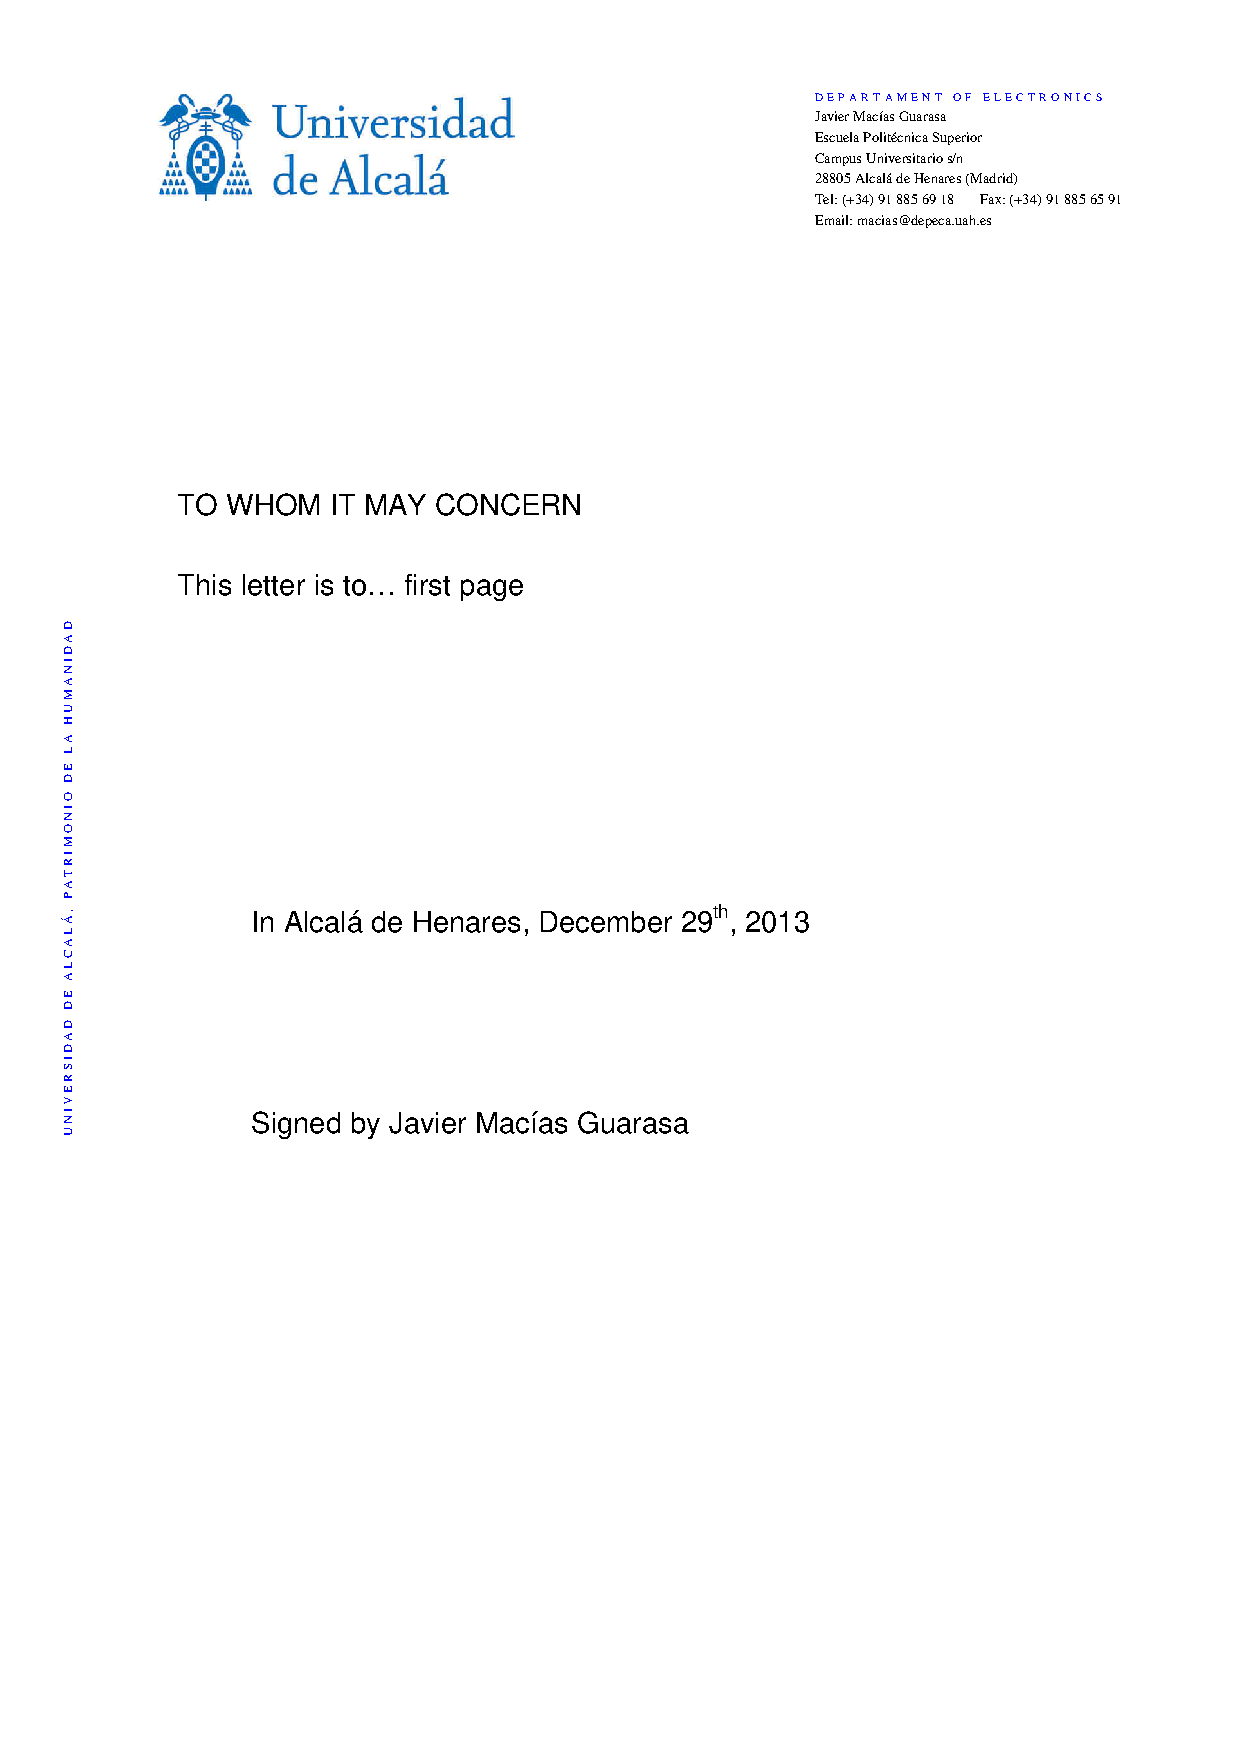
\includepdf[pages=-]{letters/sampleLetter-pages.pdf}   % include all pages of
%                                                 % pdf file
\clearemptydoublepage % You need to add this after including each pdf

%\includepdf[pages=-]{papeleo/vistoBuenoTutorTFM-MUSEA.pdf}   % for TFMs
%\clearemptydoublepage % You need to add this after including each pdf

% Dedication+ackowledgements (dedicatorias+agradecimientos)
%%%%%%%%%%%%%%%%%%%%%%%%%%%%%%%%%%%%%%%%%%%%%%%%%%%%%%%%%%%%%%%%%%%%%%%%%%% 
% 
% Generic template for TFC/TFM/TFG/Tesis
% 
% $Id: dedicatoria.tex,v 1.5 2015/06/05 00:10:35 macias Exp $
% 
% By:
% + Javier Macías-Guarasa. 
% Departamento de Electrónica
% Universidad de Alcalá
% + Roberto Barra-Chicote. 
% Departamento de Ingeniería Electrónica
% Universidad Politécnica de Madrid   
% 
% Based on original sources by Roberto Barra, Manuel Ocaña, Jesús Nuevo,
% Pedro Revenga, Fernando Herránz and Noelia Hernández. Thanks a lot to
% all of them, and to the many anonymous contributors found (thanks to
% google) that provided help in setting all this up.
% 
% See also the additionalContributors.txt file to check the name of
% additional contributors to this work.
% 
% If you think you can add pieces of relevant/useful examples,
% improvements, please contact us at (macias@depeca.uah.es)
% 
% You can freely use this template and please contribute with
% comments or suggestions!!!
% 
%%%%%%%%%%%%%%%%%%%%%%%%%%%%%%%%%%%%%%%%%%%%%%%%%%%%%%%%%%%%%%%%%%%%%%%%%%% 

% 
% This is also courtesy of Roberto Barra
% 
% To center text in a page:
% \topskip0pt
% \vspace*{\fill}
% text
% \vspace*{\fill}

\thispagestyle{empty}

\begin{flushright}

  \topskip0pt
  \vspace*{\fill}

  \textbf{A mi Madre, allá donde esté ...\ldots}\\

  \vspace{3cm}

  \emph{``En este vasto mundo \\
  	navegáis en pos de un sueño,  \\
  	surcando el ancho mar  \\
  	que se extiende frente a vosotros.  \\
  	El puerto de destino es el mañana  \\
  	cada día más incierto.  \\
  	Encontrad el camino,  \\
  	cumplid vuestros sueños,  \\
  	estáis todos en el mismo barco  \\
  	y vuestra bandera es la libertad”  \\
  	Espero que te guste Mamá, allá donde estés …''}\\ 
    Opening 3 de One Piece. \\
    Autor: The Babystars

\end{flushright}  

\vspace{4cm}
\vspace*{\fill}

% \clearemptydoublepage



%%% Local Variables:
%%% TeX-master: "../book"
%%% End:
            % EDIT this file or
                                              % comment it out
                                              
%%%%%%%%%%%%%%%%%%%%%%%%%%%%%%%%%%%%%%%%%%%%%%%%%%%%%%%%%%%%%%%%%%%%%%%%%%%
%
% Generic template for TFC/TFM/TFG/Tesis
%
% $Id: agradecimientos.tex,v 1.7 2015/06/05 00:10:31 macias Exp $
%
% By:
%  + Javier Macías-Guarasa. 
%    Departamento de Electrónica
%    Universidad de Alcalá
%  + Roberto Barra-Chicote. 
%    Departamento de Ingeniería Electrónica
%    Universidad Politécnica de Madrid   
% 
% Based on original sources by Roberto Barra, Manuel Ocaña, Jesús Nuevo,
% Pedro Revenga, Fernando Herránz and Noelia Hernández. Thanks a lot to
% all of them, and to the many anonymous contributors found (thanks to
% google) that provided help in setting all this up.
%
% See also the additionalContributors.txt file to check the name of
% additional contributors to this work.
%
% If you think you can add pieces of relevant/useful examples,
% improvements, please contact us at (macias@depeca.uah.es)
%
% You can freely use this template and please contribute with
% comments or suggestions!!!
%
%%%%%%%%%%%%%%%%%%%%%%%%%%%%%%%%%%%%%%%%%%%%%%%%%%%%%%%%%%%%%%%%%%%%%%%%%%%

% Use this if you don't like the fancy style
\thispagestyle{empty}

\ifthenelse{\equal{\myLanguage}{english}}
{
  \chapter*{Acknowledgements}
  \label{cha:acknowledgements}
  \markboth{Acknowledgements}{Acknowledgements}
  \addcontentsline{toc}{chapter}{Acknowledgements}
}
{
  \chapter*{Agradecimientos}
  \label{cha:agradecimientos}
  \markboth{Agradecimientos}{Agradecimientos}
  \addcontentsline{toc}{chapter}{Agradecimientos}
}

% ``Más vale un minuto de ilusión que mil horas de
% razonamiento''... (cortesía de Roberto Barra)


Esta Tesis Doctoral supone el culmen a cuatro años (Abril 2019 - Abril 2023) realmente duros, cargado de emociones, triunfos, pandemias, estafas y tropiezos, todo a partes iguales. Este es probablemente (aunque como diría Sean Connery interpretando a James Bond en 1983, \textit{Never Say Never Again}) mi último gran documento individual, académicamente hablando. Durante mi etapa universitaria (2013 hasta el momento, 2023) he tenido ciertos momentos puntuales en los que he sentido un salto cualitativo como profesional: El primero fue en el segundo cuatrimestre de segundo de carrera, cuando las cosas se pusieron tensas con Control II e Informática Industrial. Vaya sudores. El segundo probablemente fue con el fallecimiento de mi madre durante mi ERASMUS+ en Irlanda. Duros y oscuros momentos, alejado de mis seres queridos. El tercer momento llega en segundo de máster, durante mi querido ERASMUS+ en Finlandia, donde compagino una estancia preciosa en Tampere con el máster y un pre-inicio de doctorado. Me equivoqué al empezar tan pronto con la beca, "queriendo cobrar" cuanto antes, en vez de terminar tranquilamente el TFM y plantear tranquilamente la tesis, pero eso no lo sabría hasta tiempo después. Por último, toda la tesis han sido sube y bajas, con mala planificación por mi parte, momentos puntuales donde me equivoqué rotundamente al no estudiar PyTorch tras el WAF 2018 tras la sugerencia de mi tutor, el no enfocarme en técnica individual hasta bien entrado el doctorado, no querer hacer nada hasta que no tuviese la teoría perfectamente asimilada, tener demasiado respeto a la Inteligencia Artificial y escurrir el bulto de mi tesis en un compañero mientras yo me dedicaba a integrar y corregir los bugs del grupo que para mí era lo fácil. Mal. Todo mal. Pero todo cambió tras mi segunda estancia, en Estados Unidos, cuando tras llorar por no entender el camino a seguir, decidí crear mi propio camino, con paciencia, fé y práctica y error compaginado con lectura de artículos, para mejorar mi confianza y autoestima, y finalmente logré empezar a entender lo que era el Deep Learning. Gracias a todos mis errores, desventuras y discusiones, a día de hoy, excepto momentos inevitables, me encuentro con muchísima capacidad en atacar prácticamente cualquier problema. Cada año, desde hace ya varios, mi primera publicación en Instagram viene seguida de la frase "Trabaja duro en silencio y deja que tu éxito haga todo el ruido". Filosofía Kaizen, de mejora y aprendizaje continuo, para así cada día entender el mundo un poquito mejor. Si toda la dedicación y estudio que he depositado en este trabajo sirven para algo en mi futuro, sé que todo el esfuerzo habrá merecido la pena.

Después de este particular monólogo, a lo cual soy muy propenso y de lo cual mis amigos y compañeros no cesan en su empeño de recordármelo, debo, como no puede ser de otra manera, dar paso a los agradecimientos.


En primer lugar, me gustaría agradecer a mis profesores del grupo RobeSafe, especialmente a mis tutores Luis Miguel Bergasa Pascual y Rafael Barea Navarro, por ofrecerme estar en el grupo (así como aguantarme) durante estos todos estos años e intentar que tuviésemos el mejor experimental setup en el laboratorio, aunque no fuese siempre sencillo. Sin dudas considero realmente interesante la temática propuesta en esta tesis doctoral, predicción de agentes en conducción autónoma, ya que entra en el plano filosófico sobre cómo razonar el futuro de los objetos y cómo podría afectar a la capacidad ejecutiva del agente que tenga que tomar una decisión. Mi mente hace tiempo que cambió y me fijo siempre que conduzco de todo lo que intento reproducir con mis estudios. Habrá que seguir esta tendencia muy de cerca en los próximos años.

A mis tutores en las estancias de doctorado, Christoph Stiller y Eduardo Molinos en el KIT y Wei Zhan y Masayoshi Tomizuka en Berkeley. Se suele decir que unas veces se gana y otras se aprende, y yo en estas estancias aprendí demasiado.

A mis compañeros, mejor dicho, amigos, de laboratorio: Javier Araluce, Rodrigo, Felipe (chavalín), Santiago, Miguel Antunes,
antiguos compañeros como Javier del Egido, Óscar, Alejandro, Eduardo, Roberto y Pablo, y a nuevos becarios como Fabio, Navil y Pablo. Gracias de corazón por estar ahí, en nuestras charlas sobre tecnología, empleos, el camino correcto a seguir y la vida en general.

A mis amigos de la universidad, especialmente a Rocío, Juan Carlos, Esther, Sergio, Pablo, Rubén y Adrián Rocandio. Aún me acuerdo de cuando empezamos con la carrera y como ahora la vida nos va perfilando poco a poco a cada uno. Os deseo lo mejor en vuestro futuro.

A mis buenos amigos Samuel y Adrián, con quien gran parte de mi vida he compartido. Con especial cariño guardo las interminables charlas sobre la vida y el futuro después de entrenar, de comer, de cenar, en el coche.

A mi familia, uno de los pilares de mi vida. A mi padre Juan Antonio y a mi madre Petra, que en paz descanse, les debo todo lo que soy y es por ello por lo que les estaré siempre agradecido. Querida madre, no se muere quien se va, sólo se muere el que se olvida, y tú nunca caerás en el olvido. A mi querida hermana-calili-chessmaster Silvia, con quien tantas regañinas he tenido, pero el cariño que nos tenemos las supera a todas. A mi perrita Nuka (a.k.a. dragón o Nuki-Nuki), cuyos paseos matutinos son probablemente el ingrediente secreto para la elaboración de esta tesis, dando rienda suelta a mi cabeza para imaginar nuevas
propuestas mientras miraba el cielo azul. 

Al resto de la familia, amigos y compañeros, gracias por todo.

Y, por último, la persona más importante de mi vida ahora mismo. Mi querida Marta, la persona más maravillosa y buena que conozco. Hemos compartido risas, lloros, besos y abrazos. Nunca me cansaré de repetirte lo suave que tienes la piel tras darte un beso en la mejilla y después hacerte de rabiar. Espero que esta situación esté dentro de un while cuya condición sea True.
"Te quiero más que ayer, pero menos que mañana. Hoy, y siempre"

Vamos a la lectura importante compañeros!

% Back to normal JIC. Use it if you set \pagestyle{myplain} above
%\pagestyle{fancy}

%%% Local Variables:
%%% TeX-master: "../book"
%%% End:  % EDIT this file or
                                              % comment it out

% If this is the case, include definitions of acronyms (it's
% included before resumen.tex and abstract.tex in case you want
% to use them here
%%%%%%%%%%%%%%%%%%%%%%%%%%%%%%%%%%%%%%%%%%%%%%%%%%%%%%%%%%%%%%%%%%%%%%%%%%%
%
% Generic template for TFC/TFM/TFG/Tesis
%
% $Id: defacronymsgl.tex,v 1.2 2015/06/05 00:10:31 macias Exp $
%
% By:
%  + Javier Macías-Guarasa. 
%    Departamento de Electrónica
%    Universidad de Alcalá
%  + Roberto Barra-Chicote. 
%    Departamento de Ingeniería Electrónica
%    Universidad Politécnica de Madrid   
% 
% Based on original sources by Roberto Barra, Manuel Ocaña, Jesús Nuevo,
% Pedro Revenga, Fernando Herránz and Noelia Hernández. Thanks a lot to
% all of them, and to the many anonymous contributors found (thanks to
% google) that provided help in setting all this up.
%
% See also the additionalContributors.txt file to check the name of
% additional contributors to this work.
%
% If you think you can add pieces of relevant/useful examples,
% improvements, please contact us at (macias@depeca.uah.es)
%
% You can freely use this template and please contribute with
% comments or suggestions!!!
%
%%%%%%%%%%%%%%%%%%%%%%%%%%%%%%%%%%%%%%%%%%%%%%%%%%%%%%%%%%%%%%%%%%%%%%%%%%%

% This file shows some examples for glossary terms

%%%%%%%%%%%%%%%%%%%%%%%%%%%%%%%%%%%%%%%%%%%%%%%%%%%%%%%%%%%%%%%%%%%%%%%%%%%
% BEGIN example of glossary terms definition
%
\newacronym{LSTM}{LSTM}{Long Short-Term Memory}
\newacronym{SOTA}{SOTA}{State-of-the-Art}
\newacronym{GAN}{GAN}{Generative Adversarial Network}
\newacronym{GNN}{GNN}{Graph Neural Network}
\newacronym{AI}{AI}{Artificial Intelligence}
\newacronym{ADE}{ADE}{Average Displacement Error}
\newacronym{FDE}{FDE}{Final Displacement Error}
\newacronym{AD}{AD}{Autonomous Driving}
\newacronym{ADS}{ADS}{Autonomous Driving Stack}
\newacronym{ITS}{ITS}{Intelligent Transportation Systems}
\newacronym{MP}{MP}{Motion Prediction}
\newacronym{BEV}{BEV}{Bird's Eye View}
\newacronym{DL}{DL}{Deep Learning}

% In the future version of texlive, we will be able to use longplural
% and shortplural. Right now we must use \newglossaryentry.

%
% END example of glossary terms definition
%%%%%%%%%%%%%%%%%%%%%%%%%%%%%%%%%%%%%%%%%%%%%%%%%%%%%%%%%%%%%%%%%%%%%%%%%%%


%%% Local Variables:
%%% TeX-master: "../book"
%%% End:
            % EDIT this file or
                                              % comment it out if you do
                                              % not use acronyms

% If this is the case, include definitions of acronyms (it's
% included before resumen.tex and abstract.tex in case you want
% to use them there
%%%%%%%%%%%%%%%%%%%%%%%%%%%%%%%%%%%%%%%%%%%%%%%%%%%%%%%%%%%%%%%%%%%%%%%%%%%
%
% Generic template for TFC/TFM/TFG/Tesis
%
% $Id: defsymbolsgl.tex,v 1.2 2015/06/05 00:10:37 macias Exp $
%
% By:
%  + Javier Macías-Guarasa. 
%    Departamento de Electrónica
%    Universidad de Alcalá
%  + Roberto Barra-Chicote. 
%    Departamento de Ingeniería Electrónica
%    Universidad Politécnica de Madrid   
% 
% Based on original sources by Roberto Barra, Manuel Ocaña, Jesús Nuevo,
% Pedro Revenga, Fernando Herránz and Noelia Hernández. Thanks a lot to
% all of them, and to the many anonymous contributors found (thanks to
% google) that provided help in setting all this up.
%
% See also the additionalContributors.txt file to check the name of
% additional contributors to this work.
%
% If you think you can add pieces of relevant/useful examples,
% improvements, please contact us at (macias@depeca.uah.es)
%
% You can freely use this template and please contribute with
% comments or suggestions!!!
%
%%%%%%%%%%%%%%%%%%%%%%%%%%%%%%%%%%%%%%%%%%%%%%%%%%%%%%%%%%%%%%%%%%%%%%%%%%%

% These ones for the symbols glossary

%%%%%%%%%%%%%%%%%%%%%%%%%%%%%%%%%%%%%%%%%%%%%%%%%%%%%%%%%%%%%%%%%%%%%%%%%%%
% BEGIN example of symbols definition
%
\newglossaryentry{ohm}{type=symbols,
        name={\ensuremath{\Omega}},
        symbol={\ensuremath{\Omega}}, 
        sort=ohm,
        description=unit of electrical resistance}

\newglossaryentry{angstrom}{type=symbols,
        name={\AA},
        symbol={\AA},
        sort=angstrom,
        description={non-SI unit of length}}

\newglossaryentry{xdet}{type=symbols,
        name={\ensuremath{x(t)}},
        symbol={\ensuremath{x(t)}},
        sort=xdet,
        description={Audio signal}}

\newglossaryentry{xidet}{type=symbols,
        name={\ensuremath{x_i(t)}},
        symbol={\ensuremath{x_i(t)}},
        sort=xidet,
        description={Audio signal captured at microphone $i$}}

\newglossaryentry{condindep}{type=symbols,
        name={\ensuremath{\ci}},
        symbol={\ensuremath{\ci}}, 
        sort=conditionalindependence,
        description=conditional independence}

%
% END example of symbols definition
%%%%%%%%%%%%%%%%%%%%%%%%%%%%%%%%%%%%%%%%%%%%%%%%%%%%%%%%%%%%%%%%%%%%%%%%%%%

%%% Local Variables:
%%% TeX-master: "../book"
%%% End:
              % EDIT this file or
                                              % comment it out if you do
                                              % not use acronyms

% Now include resumen and abstract
%%%%%%%%%%%%%%%%%%%%%%%%%%%%%%%%%%%%%%%%%%%%%%%%%%%%%%%%%%%%%%%%%%%%%%%%%%%
%
% Generic template for TFC/TFM/TFG/Tesis
%
% $Id: resumen.tex,v 1.9 2015/06/05 00:10:31 macias Exp $
%
% By:
%  + Javier Macías-Guarasa. 
%    Departamento de Electrónica
%    Universidad de Alcalá
%  + Roberto Barra-Chicote. 
%    Departamento de Ingeniería Electrónica
%    Universidad Politécnica de Madrid   
% 
% Based on original sources by Roberto Barra, Manuel Ocaña, Jesús Nuevo,
% Pedro Revenga, Fernando Herránz and Noelia Hernández. Thanks a lot to
% all of them, and to the many anonymous contributors found (thanks to
% google) that provided help in setting all this up.
%
% See also the additionalContributors.txt file to check the name of
% additional contributors to this work.
%
% If you think you can add pieces of relevant/useful examples,
% improvements, please contact us at (macias@depeca.uah.es)
%
% You can freely use this template and please contribute with
% comments or suggestions!!!
%
%%%%%%%%%%%%%%%%%%%%%%%%%%%%%%%%%%%%%%%%%%%%%%%%%%%%%%%%%%%%%%%%%%%%%%%%%%%

\chapter*{Resumen}
\label{cha:resumen}
\markboth{Resumen}{Resumen}

\addcontentsline{toc}{chapter}{Resumen}

La conducción autónoma es considerada como una de los más grandes retos tecnológicos actuales. Cuando los coches autónomos conquisten nuestras carreteras, los accidentes se reducirán notablemente, hasta casi desaparecer, ya que la tecnología estará testada y no incumplirá las normas de conducción, entre otros beneficios sociales y económicos.

Uno de los aspectos más críticos a la hora de desarrollar un vehículo autónomo es percibir y entender la escena que le rodea. Esta tarea debe ser tan precisa y eficiente como sea posible para posteriormente predecir el futuro de esta misma y ayudar a la toma de decisiones. De esta forma, las acciones tomadas por el vehículo garantizarán tanto la seguridad del vehículo en sí mismo y sus ocupantes, como la de los obstáculos circundantes, tales como viandantes, otros vehículos o infraestructura de la carretera.

En ese sentido, esta tesis doctoral se centra en el estudio y desarrollo de distintas técnicas predictivas para el entendimiento de la escena en el contexto de la conducción autónoma. Durante la tesis, se observa una incorporación progresiva de técnicas de aprendizaje profundo en los distintos algoritmos propuestos para mejorar el razonamiento sobre qué está ocurriendo en el escenario de tráfico así como modelar las complejas interacciones entre la información social (distintos participantes o agentes del escenario, tales como vehículos, ciclistas o peatones) y física (es decir, la información geométrica, semántica y topológica del mapa de alta definición) presente en la escena. 

La capa de percepción de un vehículo autónomo se divide modularmente en tres etapas: Detección, Monitorización y Predicción. Para iniciar el estudio de las etapas de monitorización y predicción, se propone un algoritmo de \textit{Multi-Object Tracking} basado en técnicas clásicas de estimación de movimiento y asociación validado en el dataset KITTI, el cual tiene métricas del estado del arte. Por otra parte, se propone el uso de un filtro inteligente basado en información contextual de mapa, cuyo objetivo es monitorizar los agentes más relevantes de la escena en el tiempo, representando estos agentes filtrados la entrada preliminar para realizar predicciones unimodales basadas en un modelo cinemático. Para validar esta propuesta de filtro inteligente se usa CARLA, uno de los simuladores hiperrealistas para conducción autónoma más prometedores en la actualidad, comprobando cómo al usar información contextual de mapa se puede reducir notablemente el tiempo de inferencia de \textit{tracking} y predicción prestando atención a los agentes realmente relevantes del escenario de tráfico.

Tras observar las limitaciones de un modelo de predicción basado en cinemática para la predicción a largo plazo de un agente, los distintos algoritmos de la tesis se centran en el módulo de predicción, usando los datasets Argoverse 1 y Argoverse 2, donde se asume que los agentes proporcionados en cada escenario de tráfico ya están monitorizados durante un cierto número de observaciones. 

En primer lugar, se introduce un modelo basado en redes neuronales recurrentes (particularmente redes LSTM, \textit{Long-Short Term Memory}) y mecanismo de atención para codificar las trayectorias pasadas de los agentes, y una representación simplificada del mapa en forma de posiciones finales potenciales en la carretera para calcular las trayectorias futuras unimodales, todo envuelto en un marco GAN (\textit{Generative Adversarial Network}), obteniendo métricas similares al estado del arte en el caso unimodal.

Una vez validado el modelo anterior en Argoverse 1, se proponen distintos modelos (sólo social, incorporando mapa, y una mejora final basada en \textit{Transformer encoder} y redes convolucionales 1D) base precisos y eficientes basados en el modelo de predicción anterior, introduciendo el uso de las redes gráficas (particularmente GCN, \textit{Graph Convolutional Network}) para codificar de una forma potente las interacciones de los agentes y el preprocesamiento de trayectorias preliminares a partir de mapa con un método heurístico, para posteriormente predecir distintas trayectorias futuras en este caso multimodales, es decir, cubriendo distintos posibles futuros para el agente de interés. Los modelos base propuestos obtienen métricas de regresión del estado del arte tanto en el caso multimodal como unimodal manteniendo un claro compromiso de eficiencia con respecto a otras propuestas.

El modelo final de la tesis, inspirado en los modelos anteriores y validado en el más reciente dataset para algoritmos de predicción en conducción autónoma (Argoverse 2), introduciendo la información topológica y semántica de los carriles futuros preliminares con el método heurístico antes mencionado, codificación de mapa basada en aprendizaje profundo con redes GCN, ciclo de fusión de características físicas y sociales, estimación de posiciones finales en la carretera con aprendizaje profundo y agregación de su entorno circundante, y finalmente módulo de refinado para mejorar la calidad de las predicciones multimodales finales de un modo elegante y eficiente. Comparado con el estado del arte, nuestro método logra métricas de predicción a la par con los métodos mejor posicionados en el Leaderboard de Argoverse 2, reduciendo de forma notable el número de parámetros y operaciones de coma flotante por segundo.

Finalmente, este modelo final es validado en simulación en distintas aplicaciones de conducción autónoma, como la toma de decisiones en el simulador SMARTS o el estudio de adaptación de dominio en el simulador hiperrealista CARLA con otras capas del vehículo como paso preliminar a su implementación en un vehículo autónomo real.

\textbf{Palabras clave:} \myThesisKeywords.

%%% Local Variables:
%%% TeX-master: "../book"
%%% End:


                  % EDIT this file
%%%%%%%%%%%%%%%%%%%%%%%%%%%%%%%%%%%%%%%%%%%%%%%%%%%%%%%%%%%%%%%%%%%%%%%%%%%
%
% Generic template for TFC/TFM/TFG/Tesis
%
% $Id: abstract.tex,v 1.9 2015/06/05 00:10:31 macias Exp $
%
% By:
%  + Javier Macías-Guarasa. 
%    Departamento de Electrónica
%    Universidad de Alcalá
%  + Roberto Barra-Chicote. 
%    Departamento de Ingeniería Electrónica
%    Universidad Politécnica de Madrid   
% 
% Based on original sources by Roberto Barra, Manuel Ocaña, Jesús Nuevo,
% Pedro Revenga, Fernando Herránz and Noelia Hernández. Thanks a lot to
% all of them, and to the many anonymous contributors found (thanks to
% google) that provided help in setting all this up.
%
% See also the additionalContributors.txt file to check the name of
% additional contributors to this work.
%
% If you think you can add pieces of relevant/useful examples,
% improvements, please contact us at (macias@depeca.uah.es)
%
% You can freely use this template and please contribute with
% comments or suggestions!!!
%
%%%%%%%%%%%%%%%%%%%%%%%%%%%%%%%%%%%%%%%%%%%%%%%%%%%%%%%%%%%%%%%%%%%%%%%%%%%

\chapter*{Abstract}
\label{cha:abstract}

\addcontentsline{toc}{chapter}{Abstract}

Autonomous driving is considered one of the greatest technological challenges of the present time. When autonomous cars take over our roads, accidents will be significantly reduced, to the point of almost disappearing, as the technology will be thoroughly tested and will not violate driving regulations, such as speeding, dangerous overtaking, or driver distractions, among other factors.

One of the most critical aspects in developing an autonomous vehicle is perceiving and understanding the surrounding scene as precisely and efficiently as possible in order to predict its future and assist in decision-making. Thus, the actions taken by the vehicle or driver, in the case of partially autonomous driving, must ensure the safety of the vehicle itself, its occupants, and the surrounding obstacles, such as pedestrians, other vehicles, or road infrastructure.

In this regard, this doctoral thesis focuses on the study and development of various predictive techniques for scene understanding in the context of autonomous driving, progressively incorporating deep learning into the proposed algorithms to improve reasoning about what is happening in the traffic scenario and model the complex interactions among different participants or agents in the scene (such as vehicles, cyclists, or pedestrians), as well as the geometric, semantic, and topological information from the high-definition map present in the scene.

Firstly, an algorithm based on classical motion estimation and association techniques is proposed, along with an intelligent filter based on contextual map information. Its objective is to monitor the different agents over time, providing a preliminary input for making predictions based on a kinematic model. This model investigates how using contextual map information can significantly reduce inference time by focusing on the truly relevant agents in the traffic scenario.

Secondly, a model based on recurrent neural networks and attention mechanism is introduced to encode the past trajectories of the agents, along with a simplified representation of the map in the form of potential final positions on the road. This model calculates uni-modal future trajectories, all within a generative adversarial network framework.

Thirdly, different accurate and efficient baselines are proposed based on the aforementioned prediction model. These models introduce the use graph neural networks to powerfully encode agent interactions and preprocess preliminary trajectories from the map using a heuristic method. They then predict various multi-modal future trajectories, covering different possible futures for the target agent.

Taking these previous points into consideration, the final model of the thesis improves upon the previous ones by incorporating enhancements in the heuristic method, including topological and semantic information of interest about lanes, deep learning-based map encoding, fusion of physical and social features, deep learning-based estimation of final positions on the road, aggregation of the surrounding environment, and refinement of predictions to enhance the quality of the final multi-modal predictions in an elegant and efficient manner.

Finally, this final model is validated in various autonomous driving applications, such as decision-making or holistic integration in a hyper-realistic simulator with other vehicle layers, as a preliminary step towards its implementation in an actual autonomous vehicle.

\textbf{Keywords:} \myThesisKeywordsEnglish.

%%% Local Variables:
%%% TeX-master: "../book"
%%% End:


                 % EDIT this file

% Just for TFGs/PFCs at UAH, I do nothing and leave to the author the
% inclusion of the file
%%%%%%%%%%%%%%%%%%%%%%%%%%%%%%%%%%%%%%%%%%%%%%%%%%%%%%%%%%%%%%%%%%%%%%%%%%%%
%
% Generic template for TFC/TFM/TFG/Tesis
%
% $Id: resumen-extendido.tex,v 1.6 2015/06/05 00:10:31 macias Exp $
%
% By:
%  + Javier Macías-Guarasa. 
%    Departamento de Electrónica
%    Universidad de Alcalá
%  + Roberto Barra-Chicote. 
%    Departamento de Ingeniería Electrónica
%    Universidad Politécnica de Madrid   
% 
% Based on original sources by Roberto Barra, Manuel Ocaña, Jesús Nuevo,
% Pedro Revenga, Fernando Herránz and Noelia Hernández. Thanks a lot to
% all of them, and to the many anonymous contributors found (thanks to
% google) that provided help in setting all this up.
%
% See also the additionalContributors.txt file to check the name of
% additional contributors to this work.
%
% If you think you can add pieces of relevant/useful examples,
% improvements, please contact us at (macias@depeca.uah.es)
%
% You can freely use this template and please contribute with
% comments or suggestions!!!
%
%%%%%%%%%%%%%%%%%%%%%%%%%%%%%%%%%%%%%%%%%%%%%%%%%%%%%%%%%%%%%%%%%%%%%%%%%%%

\ifthenelse{\equal{\myLanguage}{english}}
{
\chapter*{Extended Abstract}
\label{cha:resumen-extendido}
\markboth{Extended Abstract}{Extended Abstract}

\addcontentsline{toc}{chapter}{Extended Abstract}
}
{
\chapter*{Resumen extendido}
\label{cha:resumen-extendido}
\markboth{Resumen extendido}{Resumen extendido}

\addcontentsline{toc}{chapter}{Resumen extendido}
}

Con un máximo de cuatro o cinco páginas. Se supone que sólo está
definido como obligatorio para los TFGs y PFCs de UAH.

%%% Local Variables:
%%% TeX-master: "../book"
%%% End:


       % EDIT this file

% Now include toc and list of figures+tables
%%%%%%%%%%%%%%%%%%%%%%%%%%%%%%%%%%%%%%%%%%%%%%%%%%%%%%%%%%%%%%%%%%%%%%%%%%%
%
% Generic template for TFC/TFM/TFG/Tesis
%
% $Id: toc+lof+lot.tex,v 1.9 2015/06/05 00:10:34 macias Exp $
%
% By:
%  + Javier Macías-Guarasa. 
%    Departamento de Electrónica
%    Universidad de Alcalá
%  + Roberto Barra-Chicote. 
%    Departamento de Ingeniería Electrónica
%    Universidad Politécnica de Madrid   
% 
% Based on original sources by Roberto Barra, Manuel Ocaña, Jesús Nuevo,
% Pedro Revenga, Fernando Herránz and Noelia Hernández. Thanks a lot to
% all of them, and to the many anonymous contributors found (thanks to
% google) that provided help in setting all this up.
%
% See also the additionalContributors.txt file to check the name of
% additional contributors to this work.
%
% If you think you can add pieces of relevant/useful examples,
% improvements, please contact us at (macias@depeca.uah.es)
%
% You can freely use this template and please contribute with
% comments or suggestions!!!
%
%%%%%%%%%%%%%%%%%%%%%%%%%%%%%%%%%%%%%%%%%%%%%%%%%%%%%%%%%%%%%%%%%%%%%%%%%%%

\hypersetup{linkcolor=\mytoclinkcolor}
\tableofcontents

\hypersetup{linkcolor=\myloflinkcolor}
\listoffigures
                          
\hypersetup{linkcolor=\mylotlinkcolor}
\listoftables

\hypersetup{linkcolor=\mylinkcolor}

%%% Local Variables:
%%% TeX-master: "../book"
%%% End:
                 % DO NOT TOUCH THIS LINE!

% If you want to include additional listings, you can use the float
% package. As an example, I include here the listing of source code
% snippets and algorithms (you have some examples in
% appendix/manual.tex)
%%%%%%%%%%%%%%%%%%%%%%%%%%%%%%%%%%%%%%%%%%%%%%%%%%%%%%%%%%%%%%%%%%%%%%%%%%%
%
% Generic template for TFC/TFM/TFG/Tesis
%
% $Id: extralistings.tex,v 1.5 2015/06/05 00:10:34 macias Exp $
%
% By:
%  + Javier Macías-Guarasa. 
%    Departamento de Electrónica
%    Universidad de Alcalá
%  + Roberto Barra-Chicote. 
%    Departamento de Ingeniería Electrónica
%    Universidad Politécnica de Madrid   
% 
% Based on original sources by Roberto Barra, Manuel Ocaña, Jesús Nuevo,
% Pedro Revenga, Fernando Herránz and Noelia Hernández. Thanks a lot to
% all of them, and to the many anonymous contributors found (thanks to
% google) that provided help in setting all this up.
%
% See also the additionalContributors.txt file to check the name of
% additional contributors to this work.
%
% If you think you can add pieces of relevant/useful examples,
% improvements, please contact us at (macias@depeca.uah.es)
%
% You can freely use this template and please contribute with
% comments or suggestions!!!
%
%%%%%%%%%%%%%%%%%%%%%%%%%%%%%%%%%%%%%%%%%%%%%%%%%%%%%%%%%%%%%%%%%%%%%%%%%%%

\begin{comment}
% Include the list of source code listings (if this is the case)
\hypersetup{linkcolor=\myothertoclinkcolor}
\ifthenelse{\equal{\myLanguage}{english}}
{
	\listof{codefloat}{List of Source Code}
	\addcontentsline{toc}{chapter}{List of Source Code}
}
{
	\listof{codefloat}{Índice de listados de código fuente}    
	\addcontentsline{toc}{chapter}{Índice de listados de código fuente}
}
\end{comment}
\begin{comment}
\ifthenelse{\equal{\myLanguage}{english}}
{
\renewcommand*{\algorithmcfname}{Algorithm}
\renewcommand{\listofalgorithms}{\begingroup
  \tocfile{List of Algorithms}{loa}
  \endgroup}
% \makeatletter
% \let\l@algorithm\l@figure
% \makeatother

}
\end{comment}
{
%\SetAlgorithmName{Algoritmo}{algoritmo}{Índice de algoritmos}
\renewcommand*{\algorithmcfname}{Algoritmo}
\renewcommand{\listofalgorithms}{\begingroup
   \tocfile{Índice de algoritmos}{loa}
   \endgroup}
 % \makeatletter
 % \let\l@algorithm\l@figure
 % \makeatother
}

\listofalgorithms

\hypersetup{linkcolor=\mylinkcolor}


%%% Local Variables:
%%% TeX-master: "../book"
%%% End:
               % Edit this file or
                                              % comment it out

% Now include list of acronyms and options (if this is the case)
%%%%%%%%%%%%%%%%%%%%%%%%%%%%%%%%%%%%%%%%%%%%%%%%%%%%%%%%%%%%%%%%%%%%%%%%%%%
%
% Generic template for TFC/TFM/TFG/Tesis
%
% $Id: acronymsgl.tex,v 1.8 2015/06/05 00:10:31 macias Exp $
%
% By:
%  + Javier Macías-Guarasa. 
%    Departamento de Electrónica
%    Universidad de Alcalá
%  + Roberto Barra-Chicote. 
%    Departamento de Ingeniería Electrónica
%    Universidad Politécnica de Madrid   
% 
% Based on original sources by Roberto Barra, Manuel Ocaña, Jesús Nuevo,
% Pedro Revenga, Fernando Herránz and Noelia Hernández. Thanks a lot to
% all of them, and to the many anonymous contributors found (thanks to
% google) that provided help in setting all this up.
%
% See also the additionalContributors.txt file to check the name of
% additional contributors to this work.
%
% If you think you can add pieces of relevant/useful examples,
% improvements, please contact us at (macias@depeca.uah.es)
%
% You can freely use this template and please contribute with
% comments or suggestions!!!
%
%%%%%%%%%%%%%%%%%%%%%%%%%%%%%%%%%%%%%%%%%%%%%%%%%%%%%%%%%%%%%%%%%%%%%%%%%%%

% You can change the way the entries appear the first time they are
% used. I've used italics by default. I found a problem if using this:
% LaTeX adds an extra space after the acronym, so I'm commenting it out
% (if you find a solution, please let me know)
%\defglsdisplayfirst[\acronymtype]{\textit{#1}} % EDIT this if required

% This may lead to problems... I don't know how to fix it in case the
% column for acronym is wider than 0.3\linewidth
\setlength{\glsdescwidth}{0.7\linewidth}       % EDIT this if required

% Set language specific definitions...
\ifthenelse{\equal{\myLanguage}{english}}
{
\printglossary[type=\acronymtype,style=super,nonumberlist=true,title=List of Acronyms,toctitle=List of Acronyms]
\addcontentsline{toc}{chapter}{List of Acronyms}
}
{
\printglossary[type=\acronymtype,style=super,nonumberlist=true,title=Lista de acrónimos,toctitle=Lista de acrónimos]
\addcontentsline{toc}{chapter}{Lista de acrónimos}
}


%%% Local Variables:
%%% TeX-master: "../book"
%%% End:


               % EDIT this file or
                                              % comment it out if you do
                                              % not use acronyms

%
% END within-document configuration, frontpage and cover pages generation
%%%%%%%%%%%%%%%%%%%%%%%%%%%%%%%%%%%%%%%%%%%%%%%%%%%%%%%%%%%%%%%%%%%%%%%%%%%

%%%%%%%%%%%%%%%%%%%%%%%%%%%%%%%%%%%%%%%%%%%%%%%%%%%%%%%%%%%%%%%%%%%%%%%%%%%
% Now start text and numbering for mainmatter (chapter+appendices)
%%%%%%%%%%%%%%%%%%%%%%%%%%%%%%%%%%%%%%%%%%%%%%%%%%%%%%%%%%%%%%%%%%%%%%%%%%%
\mainmatter                                       % DO NOT TOUCH THIS LINE!
\deactivatetilden                                 % DO NOT TOUCH THIS LINE!

%%%%%%%%%%%%%%%%%%%%%%%%%%%%%%%%%%%%%%%%%%%%%%%%%%%%%%%%%%%%%%%%%%%%%%%%%%%
%%%%%%%%%%%%%%%%%%%%%%%%%%%%%%%%%%%%%%%%%%%%%%%%%%%%%%%%%%%%%%%%%%%%%%%%%%%
%%%%%%%%%%%%%%%%%%%%%%%%%%%%%%%%%%%%%%%%%%%%%%%%%%%%%%%%%%%%%%%%%%%%%%%%%%%
%%%%%%%%%%%%%%%%%%%%%%%%%%%%%%%%%%%%%%%%%%%%%%%%%%%%%%%%%%%%%%%%%%%%%%%%%%%
%%%%%%%%%%%%%%%%%%%%%%%%%%%%%%%%%%%%%%%%%%%%%%%%%%%%%%%%%%%%%%%%%%%%%%%%%%%
%%%%%%%%%%%%%%%%%%%%%%%%%%%%%%%%%%%%%%%%%%%%%%%%%%%%%%%%%%%%%%%%%%%%%%%%%%%
%%%%%%%%%%%%%%%%%%%%%%%%%%%%%%%%%%%%%%%%%%%%%%%%%%%%%%%%%%%%%%%%%%%%%%%%%%%
% BEGIN Normal chapters. Edit/modify all within this section
%
% I don't recommend it, but if you want to define "parts", use this...
% BEWARE: I didn't write the english dependent code
%\part*{Memoria}
%\label{part:memoria}

%%%%%%%%%%%%%%%%%%%%%%%%%%%%%%%%%%%%%%%%%%%%%%%%%%%%%%%%%%%%%%%%%%%%%%%%%%% 
% 
% Generic template for TFC/TFM/TFG/Tesis
% 
% By:
% + Javier Macías-Guarasa. 
% Departamento de Electrónica
% Universidad de Alcalá
% + Roberto Barra-Chicote. 
% Departamento de Ingeniería Electrónica
% Universidad Politécnica de Madrid   
% 
% Based on original sources by Roberto Barra, Manuel Ocaña, Jesús Nuevo,
% Pedro Revenga, Fernando Herránz and Noelia Hernández. Thanks a lot to
% all of them, and to the many anonymous contributors found (thanks to
% google) that provided help in setting all this up.
% 
% See also the additionalContributors.txt file to check the name of
% additional contributors to this work.
% 
% If you think you can add pieces of relevant/useful examples,
% improvements, please contact us at (macias@depeca.uah.es)
% 
% You can freely use this template and please contribute with
% comments or suggestions!!!
% 
%%%%%%%%%%%%%%%%%%%%%%%%%%%%%%%%%%%%%%%%%%%%%%%%%%%%%%%%%%%%%%%%%%%%%%%%%%% 

\chapter{Introduction}
\label{cha:introduction}

\begin{FraseCelebre}
  \begin{Frase}
    Aaay, el oro, la fama, el poder.  \\
    Todo lo tuvo el hombre que en su día se autoproclamó  \\
    el rey de los piratas, ¡GOLD ROGER!  \\
    Mas sus últimas palabras no fueron muy afortunadas:  \\
    "¿¡MI TESORO!? Lo dejé todo allí, buscadlo si queréis,  \\
    ojalá se le atragante al rufián que lo encuentre.
  \end{Frase}
  \begin{Fuente}
    Opening 1 de One Piece: "We are" \\
    Autor original: Hiroshi Kitadani
  \end{Fuente}
\end{FraseCelebre}

\section{Motivation}
\label{sec:1_motivation}

\ac{AD} have held the attention of technology enthusiasts and futurists for some time as evidenced by the continuous research and development in \ac{ITS} over the past decades, being one of the emerging technologies of the \textit{Fourth Industrial Revolution}, and particularly of the Industry 4.0. \\

The concept \textit{Fourth Industrial Revolution} or Industry 4.0  was first introduced by Klaus Schwab , CEO (Chief Executive Officer) of the World Economic Forum, in a 2015 article in Foreign Affairs (American magazine of international relations and United States foreign policy). A technological revolution can be defined as a period in which one or more technologies are replaced by other kinds of technologies in a short amount of time. Hence, it is an era of accelerated technological progress featured by Researching, Development and Innovation whose rapid application and diffusion cause an abrupt change in society. In particular, the \textit{Fourth Industrial Revolution} conceptualizes rapid change to industries, technology, processes and societal patterns in the 21st century due to increasing inter-connectivity and smart automation. This industrial revolution focuses on operational efficiency, being the following four themes which summarize it: \\

\begin{itemize}
	\item Decentralized decisions: Ability of cyber physical systems to make decisions on their own and to perform their tasks as autonomously as possible.
	\item Information transparency: Provide operators with comprehensive information to make decisions. Inter-connectivity allows operators to gather large amounts of information and data from all points in the manufacturing process in order to identify key areas or aspects that can benefit from improvement to enhance functionality.
	\item Technical assistance: Ability to assist humans with unsafe or difficult tasks and technological facility of systems to help humans in problem-solving and decision-making.
	\item Interconnection: Ability of machines, sensors, devices and people to communicate and conect with each other via the Internet of Things (IoT) or the Internet of People (IoP).
\end{itemize}

Based on the aforementioned principles, this revolution is expected to be marked by breakthroughs in emerging technologies in fields such as nanotechnology, quantum computing, 3D printing, Internet of Things (IoT), fifth-generation wireless technologies (5G), Robotics, Computer Vision (CV), \ac{AI} or the scope of this PhD thesis, \acp{ADS}. The sum of all these advances are resulting in machines that can potentially see, hear and what is more important, think, moving more deftly than humans. \\

An \ac{ADS}, also referred in the literature as Intelligent Vehicle (IV), driverless car or autonomous car, is a vehicle tan can sense its surrounding and moving safely with little or even no human input. These \acp{ADS} must combine a variety of sensors to understand the traffic scenario, like RADAR (RAdio Detection A Ranging), LiDAR (Light Detection and Ranging), cameras, Inertial Measurement Unit (IMU), wheel odometry, GNSS (Global Navigation Satellite System) or ultrasonic sensors, and detect, track and predict (which is the main purpose of this thesis) the most relevant obstacles around the ego-vehicle. Then, advanced control and planning systems process this sensory information in combination with a predefined global route to calculate the corresponding control commands to drive throughout the environment, ensuring a safe driving. \\

The dream of seeing fleets of \acp{ADS} efficiently delivering goods and people to their destination has fueled billions of dollars and captured consumer's imaginations in investment in recent years. Nevertheless, according to the "Autonomous driving's future: Convenient and connected" report, published by the global management consulting firm McKinsey \& Company in January 2023, even after some setbacks have pushed out timelines for \ac{AD} launches and delayed customer adoption, the transportation community still broadly agrees that \ac{AD} has the potential to transform consumer behaviour, transportation and society at large. \ac{AD} is considered as one of the solutions to the aforementioned problems and one of the greatest challenges of the automotive industry today. \\

Statistics show that 69 \% of the population in the European Union (EU), including associated states, lives in urban areas. According to the World Health Organization, nearly one third of the world population will live in cities by 2030, leading to an overpopulation in most of them. Aware of this problem, the Transport White Paper published by the European Commission in 2011 indicated that new forms of mobility ought to be proposed so as to provide sustainable solutions for people and goods safely. For example, regarding safety, it sets the ambitious goal of halving the overall number of road deaths in the EU between 2010 and 2020. Nevertheless, this goal does not seem to be easy since only in 2014 more than 25,700 people died on the roads in the EU, many of them caused by an improper behaviour of the driver on the road. A similar study made by the National Highway Traffic Safety Administration (NHTSA, tranportation organization of the United States) reported in 2015 that around 94 \% of traffic accidents happen because of human error. In that sense, the existence of reliable and economically affordable \acp{ADS} are expected to create a huge impact on society affecting social, demographic, environmental and economic aspects. It can produce substantial value for the auto industry, drivers and society, making driving safer, more convenient and more enjoyable. While the human driver or not could select whether to drive, in autonomous mode hours on the road previously spent driving could be used to work, watch a funny movie or even to video call a friend. For employees with long commutes, \ac{AD} might shorten the workday, increasing worker productivity. Since workers, specially those related to digital jobs or related fields, may perform their jobs from an \ac{ADS}, they could more easily move further away from the office, which, in turn, could attract more people to suburbs and rural areas. Besides this, it is estimated to cause a reduction in road deaths, reduce fuel consumption and harmful emission associated and improve traffic flow, as well as an improvement in the overall driver comfort and mobility in groups with impaired faculties, such as disable or elderly people, providing them with mobility options that go beyond car-sharing services or public transportation. Other industrial applications of autonomous vehicles are agriculture, retail, manufacturing, commercial and freight transport or mining. \\

\section{Historical Context}
\label{sec:1_historical_context}

\acp{ADS} have become a challenge for auto competitions and technology companies, which has derived in an intense competition. Though today companies such as Mercedes, Ford or Tesla are racing to build \acp{ADS} for a radically changing consumer world, the research and development of autonomous robots is not new. \\

In 1500, centuries before the invention of the automobile, Leonardo da Vinci designed a cart that could move without being pulled or pushed. In 1868, Robert Whitehead invented a torpedo that could propel itself underwater in order to be a game-changer for naval fleets all over the world. In terms of robotic solutions for intelligent mobility, the study was started in the 1920s, being the concept of Autonomous Car defined in Futurama, an exhibit at the 1939 New York Wolrd's Fair. General Motors created the exhibit to display its vision of what the world would look like in 20 years, including an automated highway system that would guide \ac{ADS}. By 1958, General Motors made this concept a reality (at least as a proof of concept) being the car's front end embedded with sensors to detect the current flowing through a wire embedded in the road. The first semi-automated car was developed in 1977 by Japan’s Tsukuba Mechanical Engineering Laboratory. The vehicle reached speeds up to 30 km/h with the support of an elevated rail. \\

\begin{figure}[h]
	\centering
	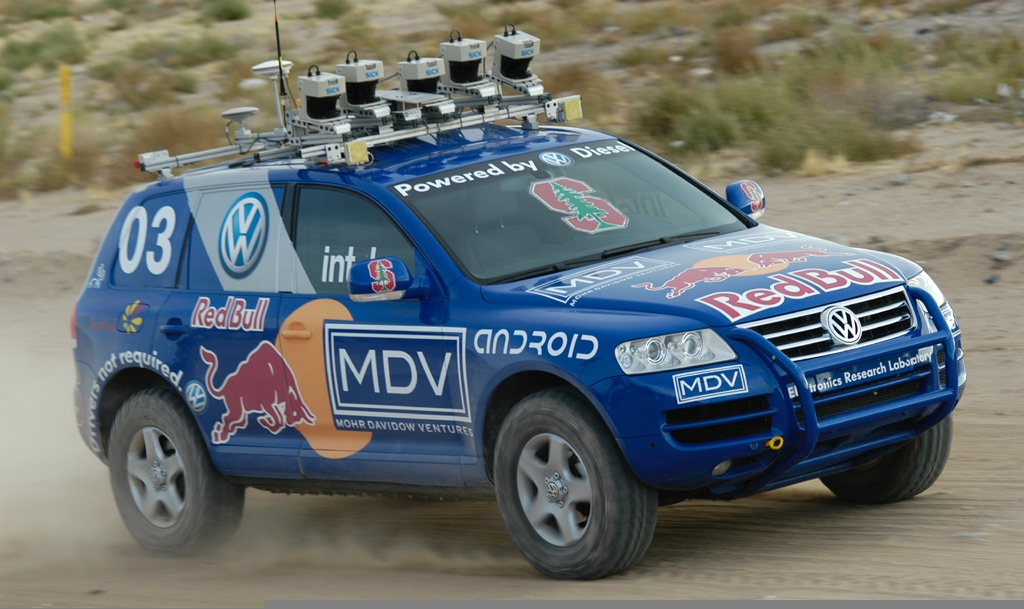
\includegraphics[width=0.8\linewidth]{1_darpa_winner_2005.png}
	\caption{Stanley, 2005 DARPA Grand Challenge winner}
	Source: \textit{Stanford university}
	\label{fig:1_darpa_winner_2005}
\end{figure}

Nevertheless, the first truly autonomous cars appeared in the 1980s with Carnegie Mellon University’s Navlab and ALV projects funded by the USA company DARPA (Defense Advanced Research Projects Agency) in 1984 and EUREKA Prometheus project (1987) developed by Mercedes-Benz and Bundeswehr University Munich’s. By 1985, the ALV project had shown self-driving speeds on two-lane roads of 31 km/h with obstacle avoidance added in 1986 and off-road driving in day and night conditions by 1987. Furthermore, from the 1960s through the second DARPA Grand Challenge in 2005 (212 km off-road course near the California-Nevada state line, surpassed by all but one of the 23 finalists), automated vehicle research in the United States was primarily funded by DARPA, the US Army and US Navy, yielding rapid advances in terms of speed, car control, sensor systems and driving competence in more complex conditions. This caused a boost in the development of autonomous prototypes by companies and research organizations, most of them from the United States. Figure \ref{fig:1_darpa_winner_2005} shows Stanley, the 2005 DARPA Gran Challenge winner, from Stanford university. \\

Even though self-driving cars have not yet displaced conventional cars, there can be found several examples of how it has become a hot topic for powerful companies such as Delphi Automotive Systems, Audi, BMW, Tesla, Mercedes-Benz or Waymo. \\

In 2005 Delphi broke the Navlab’s record achievement (driving 4,584 km while remaining 98 \% of the time autonomously) by piloting an Audi, improved with Delphi technology, over 5,472 km through 15 states while remaining in self-driving mode 99 \% of the time. Moreover, in 2005 the USA states of Michigan, Virginia, California, Florida, Nevada and the capital, Washington D.C., allowed the testing of automated cars on public roads. \\

In 2017, Audi stated that its A8 car prototype would be automated at speeds up to 60 km/h by using its perception system named “Audi AI”.  Also, in 2017 Waymo (self-driving technology development company subsidiary of Alphabet Inc) started a limited trial of a self-driving taxi service in Phoenix, Arizona. \\

Figure \ref{fig:1_disengagement_2020} shows the total number of autonomous test miles and miles per disengagement in California (Dec 2019 - Nov 2020) by some of the most important \ac{AD} technology development companies around the world. The concept disengagement is quite useful to assess the quality of an \ac{ADS}, defined as the deactivation of the autonomous mode when a failure of the autonomous technology is detected or when a safe operation requires that the autonomous vehicle test driver disengages the autonomous mode, resulting in control being seized by the human driver.

\begin{figure}[ht]
	\centering
	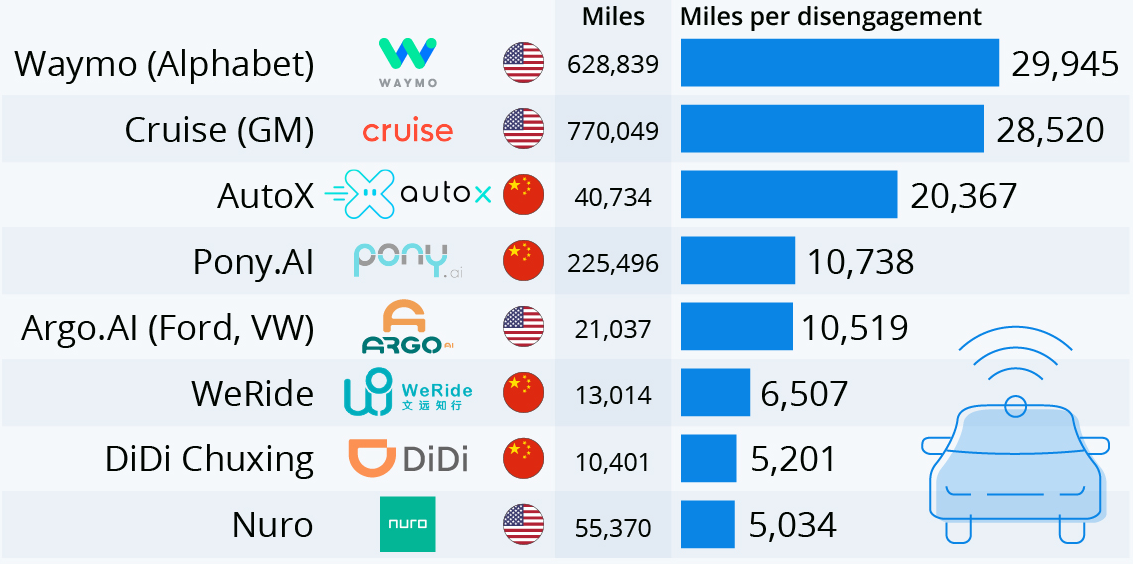
\includegraphics[width=0.6\linewidth]{1_disengagement_2020.png}
	\caption{Number of autonomous test miles and miles per disengagement (Dec 2019 - Nov 2020)}
	Source: \textit{DMV California, via The Last Driver License Holder}
	\label{fig:1_disengagement_2020}
\end{figure}

At the moment of writing this thesis (2023), many vehicles on the road are considered to be semi-autonomous due to safety features like braking systems, assisted parking, lane boundaries detection or predict the long-term behaviour of the users around the vehicle to execute the most optimal action in a safely way. Regarding this, the Society of Automotive Engineers (SAE) published the concept of autonomy levels in 2014, as part of its "Taxonomy and Definitions for Terms Related to On-Road Motor Vehicle Automated Driving Systems" report. Figure \ref{fig:1_nhtsa_sae_automation_levels} illustrates the six levels of autonomy (the higher the level, the more autonomous the car is), where it can be appreciated that Level Zero means "No Automation", being the acceleration, braking and steering controlled by a human driver at all times, and Level Five represents Full Automation, where there is a full-time automation of all driving tasks on any road, under any conditions, whether there is a human on board or not.

\begin{figure}[h]
	\centering
	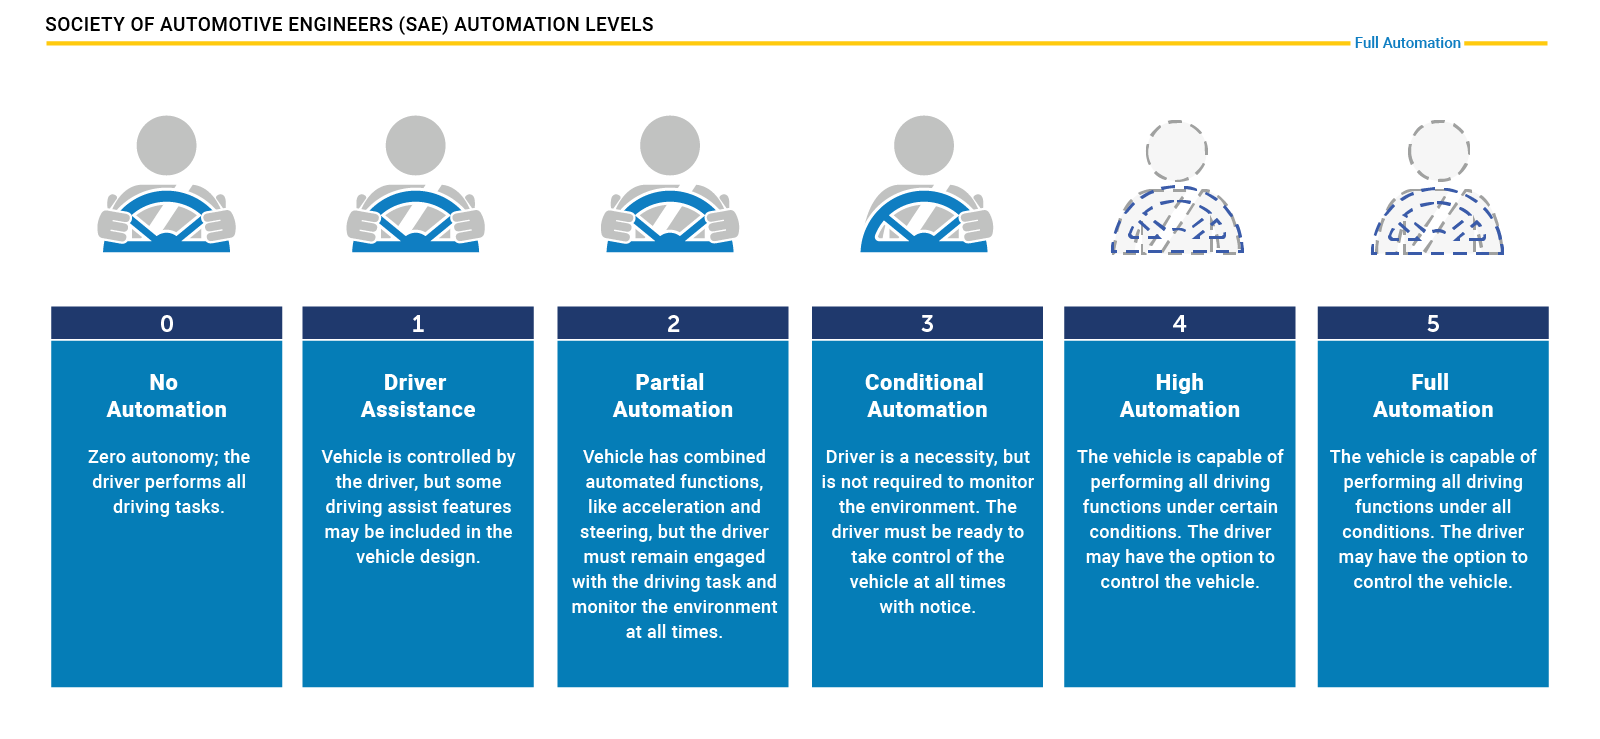
\includegraphics[width=0.8\linewidth]{1_nhtsa_sae_automation_levels.png}
	\caption{Society of Automotive Engineers (SAE) automation levels}
    Source: \textit{NHTSA (National Highway Traffic Safety Administration)}
	\label{fig:1_nhtsa_sae_automation_levels}
\end{figure}

In that sense, today most vehicles only included basic Advanced Driver Assistance Systems (ADAS), but major advancements in AD capabilities are on the horizon. According to a 2021 McKinsey consumer survey, growing demand for \ac{AD} systems could create billions of dollars in revenue. Based on a consumer interest in \ac{AD} features and commercial solutions available on the market today, ADAS and AD could generate between \$300 and \$400 billions in the passenger car market by 2035. Figure \ref{fig:1_mckinsey_revenues_ad} illustrates an interesting study reporting the revenues of ADAS and AD from Level 1 (Driver Assistance) to Level 4 (High Automation). As expected, Level 5 is excluded from this study due to the huge difficulties the automotive companies would have to face to adapt their systems under totally different environmental conditions.

\begin{figure}[h]
	\centering
	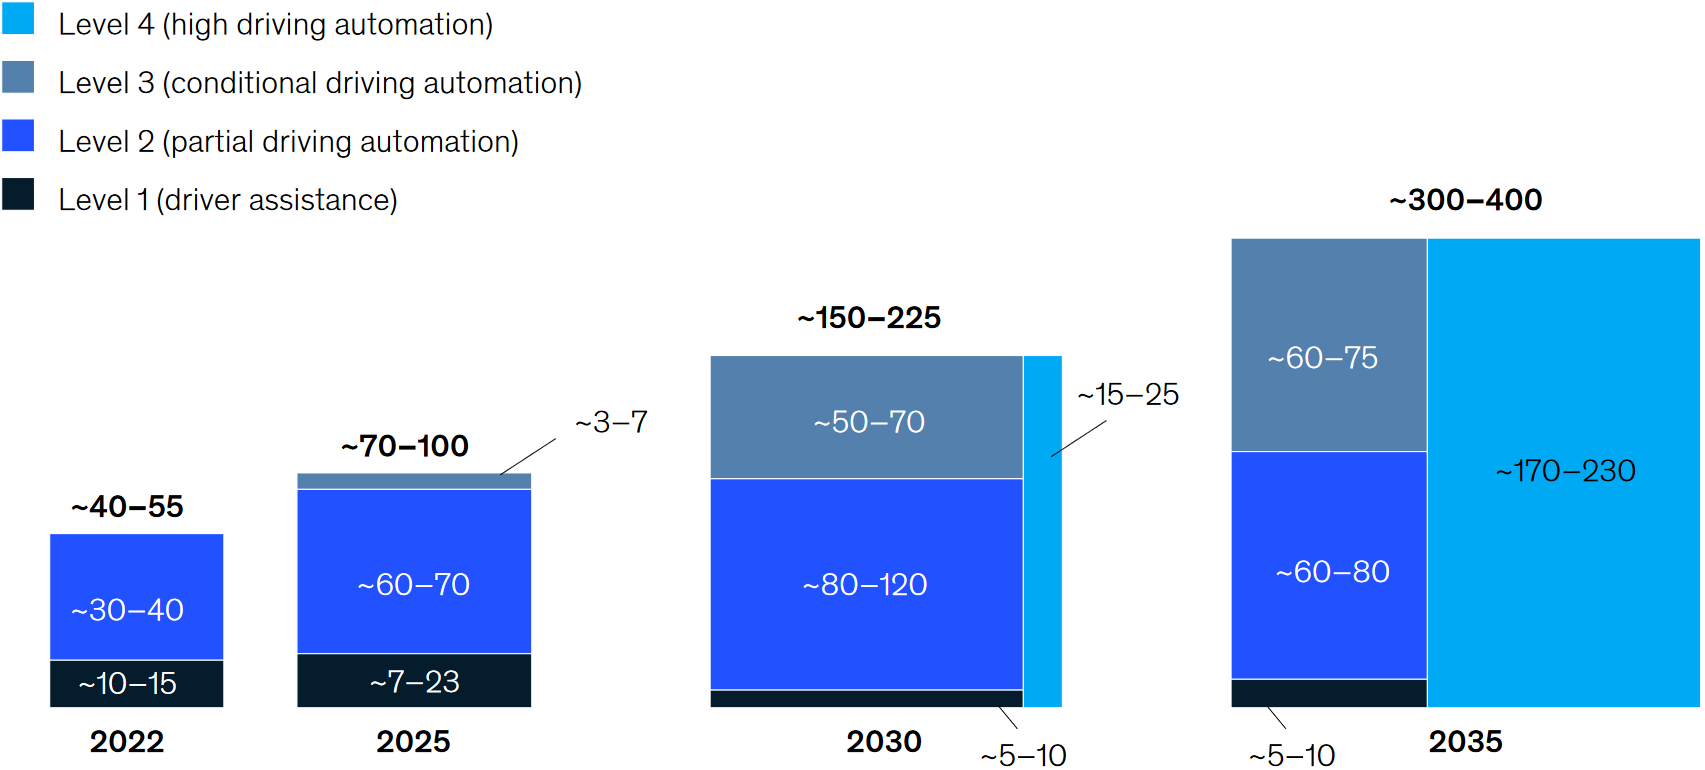
\includegraphics[width=0.8\linewidth]{1_mckinsey_revenues_ad.png}
	\caption{Advanced Driver Assistance systems (ADAS) and \\ Autonomous Driving (AD) revenues in \$ billion} Source: \textit{McKinsey Center for Future Mobility}
	\label{fig:1_mckinsey_revenues_ad}
\end{figure}

\section{Autonomous Driving architecture}
\label{sec:1_ad_architecture}

To sum up what commented above, increasing the level of autonomous navigation in mobile robots (from agriculture to public and private transport) are expected to create tangible business benefits to those users and companies employing them. However, designing an autonomous navigation system does not seem to be an easy task. In the \ac{SOTA} we can distinguish two main kind of software architectures: End-to-End and modular. Figure \ref{fig:1_ete_modular} illustrates the entire \ac{AD} architecture starting from sensing, all the way to longitudinal (throttle/brake) and lateral (steering angle) control of the vehicle, which are the commanded signals that feed the low-level electronic system that moves the vehicle, like a drive-by-wire system \cite{arango2020drive}. End-to-End are considered black-box models, where a single neural network performs the driving task (throttle/steering/brake) from raw sensor data, in such a way the error be may vanished since intermediate representations are jointly optimized, but these are not very interpretable. On the other hand, modular architectures (considered as glass models as counterpart to End-to-End approaches) separate the driving task into individually programmed or trained modules. This solution is more interpretable, since the know-how of a research group or company is easily transferred, they allow parallel development, being the standard solution in industrial research, but the error is propagated, where intermediate representations can led to suboptimal performance. For example, incorrect object detection can lead to low-quality tracking and motion prediction.

\begin{figure}[h]
	\centering
	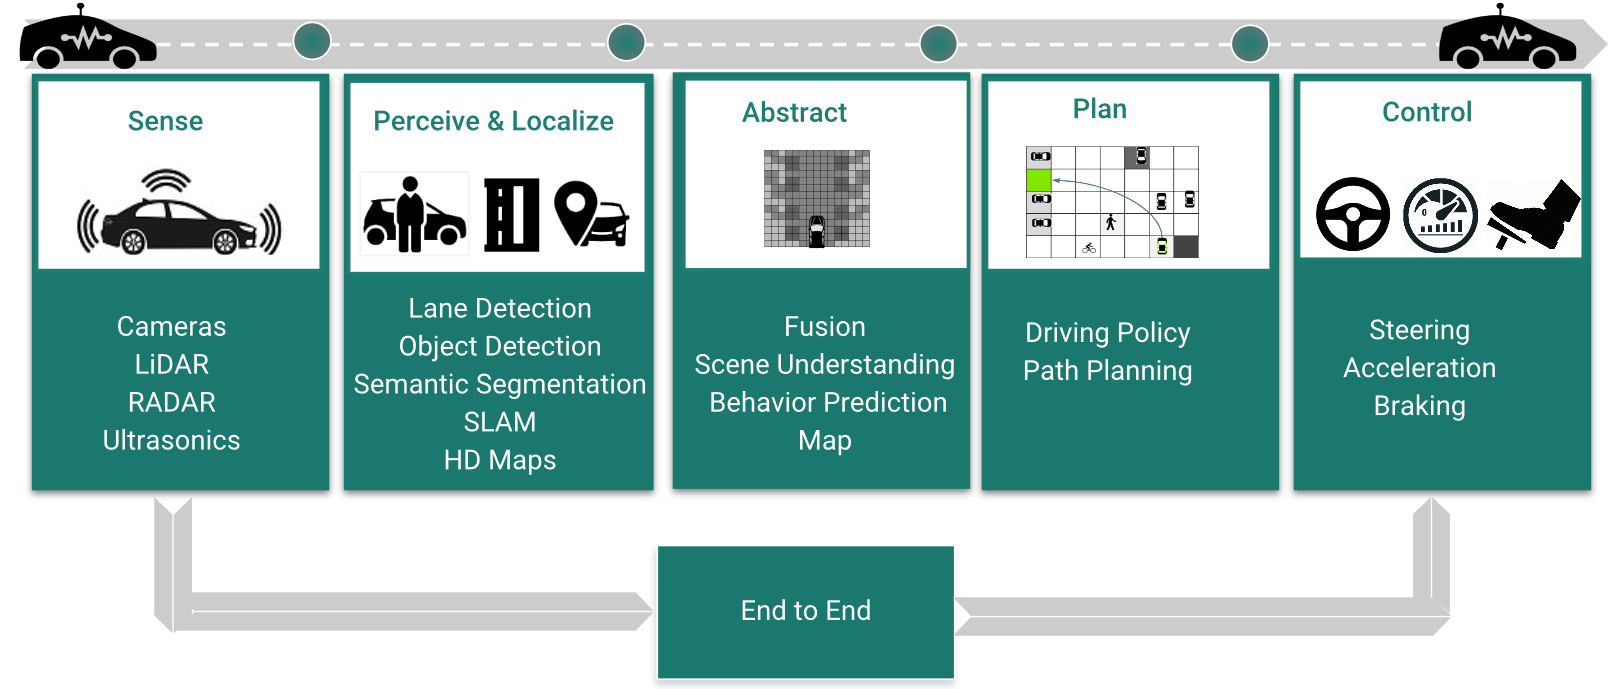
\includegraphics[width=0.8\linewidth]{1_ete_modular.png}
	\caption{Autonomous Driving Stack (ADS) modular vs end-to-end pipeline}
	Source: \textit{Vrunet: Multi-task learning model for intent prediction of vulnerable road users} \cite{ranga2020vrunet}
	\label{fig:1_ete_modular}
\end{figure}

Considering the RobeSafe (Robotics and eSafety) research group and the main projects (Techs4AgeCar, AIVATAR) where this thesis has been developed, we integrate our algorithms in a software modular approach. An example of a software modular approach is shown in Figure \ref{fig:1_pylot_architecture}. Despite the fact in literature some authors disagree on the specific software architecture of an \ac{ADS}, specially the motion prediction module, which is usually classified as a perception algorithm but sometimes is included as part of the planning or decision-making layers, we can hierarchically break down (from raw data to the driving task) a standard \ac{AD} architecture into the following software layers:

\begin{itemize}
	\item Localization layer: Positions and locates the vehicle on a map with real-time and centimetric accuracy approach. The main source of information is a robust differential-GNSS, though IMUs, wheel odometry and even cameras are commonly employed. 
	\item Perception layer: Understand the environment around the ego-vehicle thanks to the information collected by the sensors. If defined as multi-stage, the perception layer first detects the most relevant obstacles, then track them over time to finalize long-term predict with plausible predictions. In order to perform object detection, LiDAR, camera and RADAR are the main sensors that provide the corresponding raw data. Additionally, HD map information is frequently used in the motion prediction tasks by most \ac{SOTA} algorithms.
	\item Mapping layer: Responsible for creating a topologic, semantic and geographical modeling of the environment through which the vehicle drives, being the HD Map graph the most common source of information.
	\item Planning layer: This layer is comprised of three components: route, behaviour and trajectory planner. The route planner computes the most optimal (in terms of distance, time and so forth and so on) global route from some predefined start and goal. It uses the localization and mapping output. On the other hand, the behaviour planner, also referred as decision-making layer by some authors, it performs high-level decision-making of driving behaviours such as lane changes or progress through intersections, mostly focused on the previously computed global route and current localization. It can be seen as an atomization of the global route in different behaviors to reach the goal. Finally, the trajectory planner, also known as local planner, generates a time schedule for how to follow a path given constraints such as position, velocity and acceleration in order to meet the previously decided behaviour and taking into account the prediction from the perception layer, avoiding obstacles in optimal direction and speed conditions.
	\item Control layer: Once the local plan is calculated, the control layer is responsible for generating the commands that are sent to the actuators. It receives as input some waypoints from the calculations made in the trajectory planner. Once these waypoints are received, most authors perform spline interpolations and a velocity profile that ensures a smooth and continous trajectory. 
\end{itemize}

\begin{figure}[h]
	\centering
	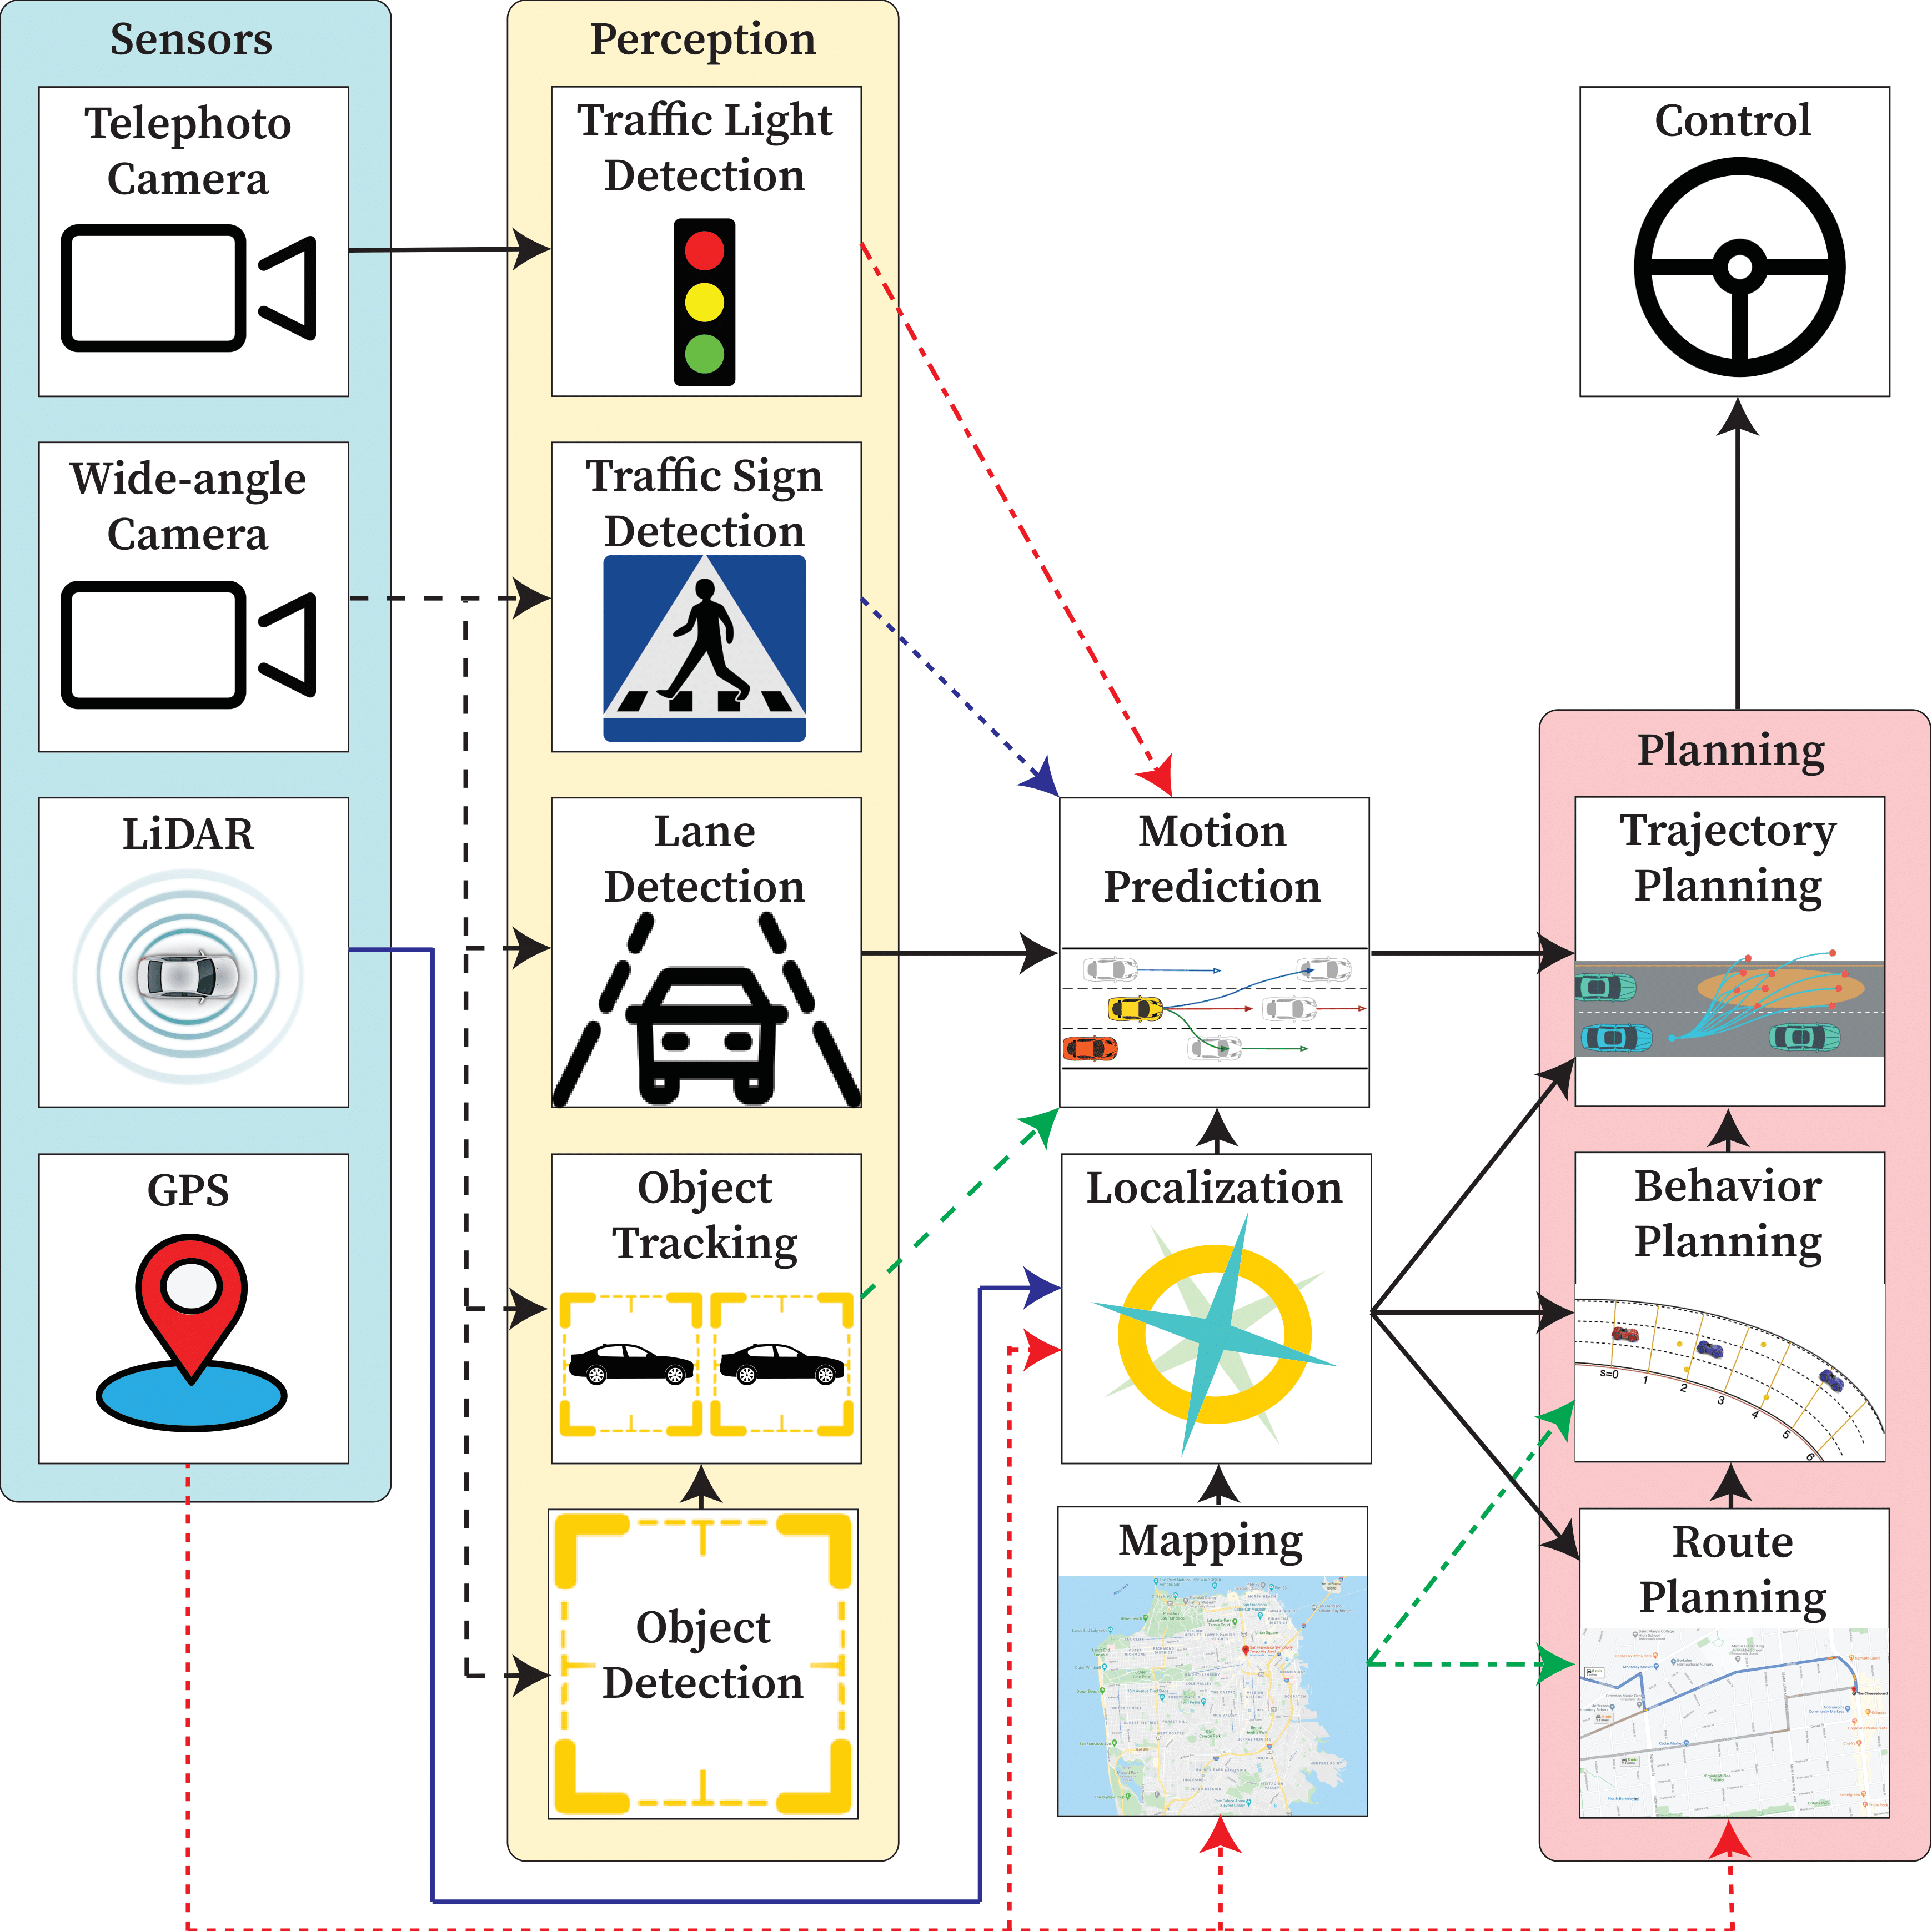
\includegraphics[width=0.8\linewidth]{1_pylot_architecture.png}
	\caption{Autonomous Driving Stack (ADS) modular pipeline}
	Source: \textit{Pylot: A modular platform for exploring latency-accuracy tradeoffs in autonomous vehicles} \cite{gog2021pylot}
	\label{fig:1_pylot_architecture}
\end{figure}

\section{Problem statement}
\label{sec:1_problem_statement}

As commented in previous sections, in order to operate efficiently and safely in highly dynamic, complex and interactive driving scenarios, \acs{ADS} need to smartly reason like human beings via predicting future motions of surrounding traffic participants during navigation. Nevertheless, achieving accurate and robust \ac{MP} in one of the most difficult and interesting challenges to achieve full-autonomy, since it is equivalent to a bridge between the former stages of the perception layer, where the scene is understood detecting and tracking static and dynamic objects of the environment, and the planning and control layer, where the future trajectory of the ego-vehicle is computed and the driving commands are sent to the physical layer (e.g. Drive-by-Wire \cite{arango2020drive}). Here are some of the most important challenges: 

\begin{enumerate}
	\item Heterogeneity of traffic participants. Traffic partipants (specially those which are dynamic) can be roughly classified as cyclists, pedestrians or other vehicles. The prediction model should be capable of differentiating the motion patterns of heterogeneous traffic participants, in such a way fine-grained classification (detection module) is quite beneficial to include additional metadata along with the past observations.
	\item Complexity of road structure. Road structures are highly diverse and complex, specially in highways and urban areas, which noticeably affect the motion behaviours of traffic participants.
	\item Variable number of interactive agents. The prediction model must deal with a number of associated traffic participants within a certain area that can vary from time to time, such as intersections or roundabouts. Then, while driving, a comprehensive representation of the scene must be able to accommodate an arbitrary number of involved traffic participants.
	\item Multimodality of driving behaviours. In real-world, despite we know the behaviour our vehicle will carry out, the motion patterns of other traffic participants can be considered inherently multimodal since there is usually more than one reasonable option for a driver to choose, specially in intersections, when the number of lanes increases or even in the same lane with different velocity profiles (constant velocity, sudden break, sudden acceleration). In that sense, a robust and reliable \ac{MP} model is expected to be human-like and capture different plausible motion modalities where an agent can travel in the prediction horizon.
	\item Complex interpendencies among traffic participants and road infrastructure. Agent-Agent, Agent-Road and Road-Road interpendencies are of great importance for \ac{MP} and interaction modeling, even more taking into account the complexity of road structures and heterogeneity of traffic participants aforementioned. As expected, an agent future trajectory will be affected not only by its own past trajectory and driving objectives (given by the behaviour planner) but also by other surrounding agents past trajectories, traffic rules and physical constraints.
\end{enumerate}

\section{Objectives and Structure of this Thesis}
\label{sec:1_objectives_and_structure}

The main scope of this thesis is to study the \ac{SOTA} and development of novel and efficient interaction-aware Deep Learning based \ac{MP} models, focusing on long-term (from 3 to 6 s) prediction horizon and \ac{AD}, where traffic participants can range from trucks to pedestrians, instead of models focused on pedestrian trajectory prediction. The main inputs that will be used throughout this work are the physical (map) information and historical states (that may include agent position, velocity, orientation, object type and category) of traffic participants in \ac{BEV}, assuming these objects have been previously tracked by our ego-vehicle (also referred as the autonomous car). Though the evaluation of these methods will be done using a single target agent, as proposed by some of the most important prediction datasets, like Argoverse 1 \cite{chang2019argoverse} and Argoverse 2 \cite{wilson2023argoverse}, some of the proposed methods will be trained considering multi-agent. In this thesis, the solutions to the aforementioned challenges will be discussed and investigated progressively. In order to achieve the main scope, the following objectives will be met:

\begin{enumerate}
	\item Research of \ac{SOTA} \ac{MP}, focused on \ac{DL} and the \ac{AD} paradigm.
	\item Propose of several \ac{MP} architectures, studying the progressive incorporation of \ac{DL} mechanisms and different sources of information and metadata, achieving \ac{SOTA} accuracy while reducing in millions of parameters previous models as well as inference time.
	\item Validate the proposed models in downstream applications, such as decision-making or behaviour planning, taking into account former stages of the perception layer (detection and tracking) instead of static files (benchmarks) in hyper-realistic simulation, as a preliminary stage before implementing it in a real-world vehicle.
\end{enumerate}

The organization of this document has been done as follows:

\begin{itemize}
	\item Chapter 2 reviews the most important features and methods of physics-based and learning-based \ac{MP} methods. The physics-based methods are reviewed according to a taxonomy similar to existing reviews. The learning-based methods are reviewed based on two classification criteria: scene representation and trajectory decoding.
	\item Chapter 3 presents a technical background, mostly focused on \ac{DL} mechanisms to deal with temporal sequences and interactions, to deeply understand the proposed methods.
	\item Chapter 4 illustrates the different prediction models developed in the thesis using different validation environments, from unimodal physic-based prediction to the final model of the thesis which takes into account agents interactions, map information and past observations using a novel scene representation with heuristic proposals, graph-based encoding, \ac{DL}-based goal proposals and motion refinement.
	\item Chapter 5 addresses the integration of the final model of the thesis with upstream and downstream modules to contribute the entire pipeline and closed-loop for \ac{AD}.
	\item Chapter 6 summarizes the thesis and provides some promising directions for future work in the areas of \ac{MP} and validation.
\end{itemize}

%%%%%%%%%%%%%%%%%%%%%%%%%%%%%%%%%%%%%%%%%%%%%%%%%%%%%%%%%%%%%%%%%%%%%%%%%%% 
% 
% Generic template for TFC/TFM/TFG/Tesis
% 
% By:
% + Javier Macías-Guarasa. 
% Departamento de Electrónica
% Universidad de Alcalá
% + Roberto Barra-Chicote. 
% Departamento de Ingeniería Electrónica
% Universidad Politécnica de Madrid   
% 
% Based on original sources by Roberto Barra, Manuel Ocaña, Jesús Nuevo,
% Pedro Revenga, Fernando Herránz and Noelia Hernández. Thanks a lot to
% all of them, and to the many anonymous contributors found (thanks to
% google) that provided help in setting all this up.
% 
% See also the additionalContributors.txt file to check the name of
% additional contributors to this work.
% 
% If you think you can add pieces of relevant/useful examples,
% improvements, please contact us at (macias@depeca.uah.es)
% 
% You can freely use this template and please contribute with
% comments or suggestions!!!
% 
%%%%%%%%%%%%%%%%%%%%%%%%%%%%%%%%%%%%%%%%%%%%%%%%%%%%%%%%%%%%%%%%%%%%%%%%%%% 

\chapter{Related Works}
\label{cha:related_works}

begin{FraseCelebre}
\begin{Frase}
	Llegaré a ser el mejor, El mejor que habrá jamás \\
	Mi causa es ser su entrenador, Tras poderlos capturar.  
	
	Viajaré a cualquier lugar, Llegaré a cualquier rincón \\  
	Y al fin podré desentrañar, El poder de su interior.  
	
	¡Pokémon! Hazte con todos (solos tú y yo), \\
	Es mi destino, mi misión \\
	¡Pokémon! Tú eres mi amigo fiel, \\
	Nos debemos defender.
\end{Frase}
\begin{Fuente}
	Opening 1 de Pokémon: "Gotta catch 'em all!" \\
	Autor original: Jason Paige
\end{Fuente}
\end{FraseCelebre}

One of the crucial tasks that \acp{ADS} must face during navigation, specially in arbitrarily complex urban scenarios, is to predict the behaviour of dynamic obstacles \cite{chang2019argoverse, salzmann2020trajectron++}. In a similar way to humans that pay more attention to nearby obstacles and upcoming turns than considering the obstacles far away, the perception layer of an \ac{ADS} must focus more on the salient regions of the scene, particularly on the more relevant dynamic agents to predict their future behaviour before conducting a maneuver, such as lane changing or accelerating. In that sense, before proceeding with the study of the different methods of the \ac{SOTA} of \ac{MP} in the field of \ac{AD}, one important thing to note is that this thesis is focused on non-conditional motion prediction, also referred as Passive Motion Prediction (PMP), where the prediction of surrounding agents is not influenced by the future decisions of the ego-vehicle or even other agents, referred as Conditional Motion Prediction (CMP) in the literature. Most existing works \cite{gilles2021home, gilles2022gohome, varadarajan2022multipath++, wang2022ganet, schmidt2022crat, liang2020learning} focus on a passive prediction scheme, where the future states of a particular agent are predicted given its past information, other surrounding agents information and interactions as well as the physical context. Then, downstream planning modules, specially the behaviour planning module (also referred as decision-making layer, as stated in Section \ref{sec:1_ad_architecture}), the ego-vehicle (our vehicle) future actions are computed according to the predicted trajectories in a passive manner, that is, without modifying the output of the prediction model, and the global route previously calculated. \\

\begin{figure}[h]
	\centering
	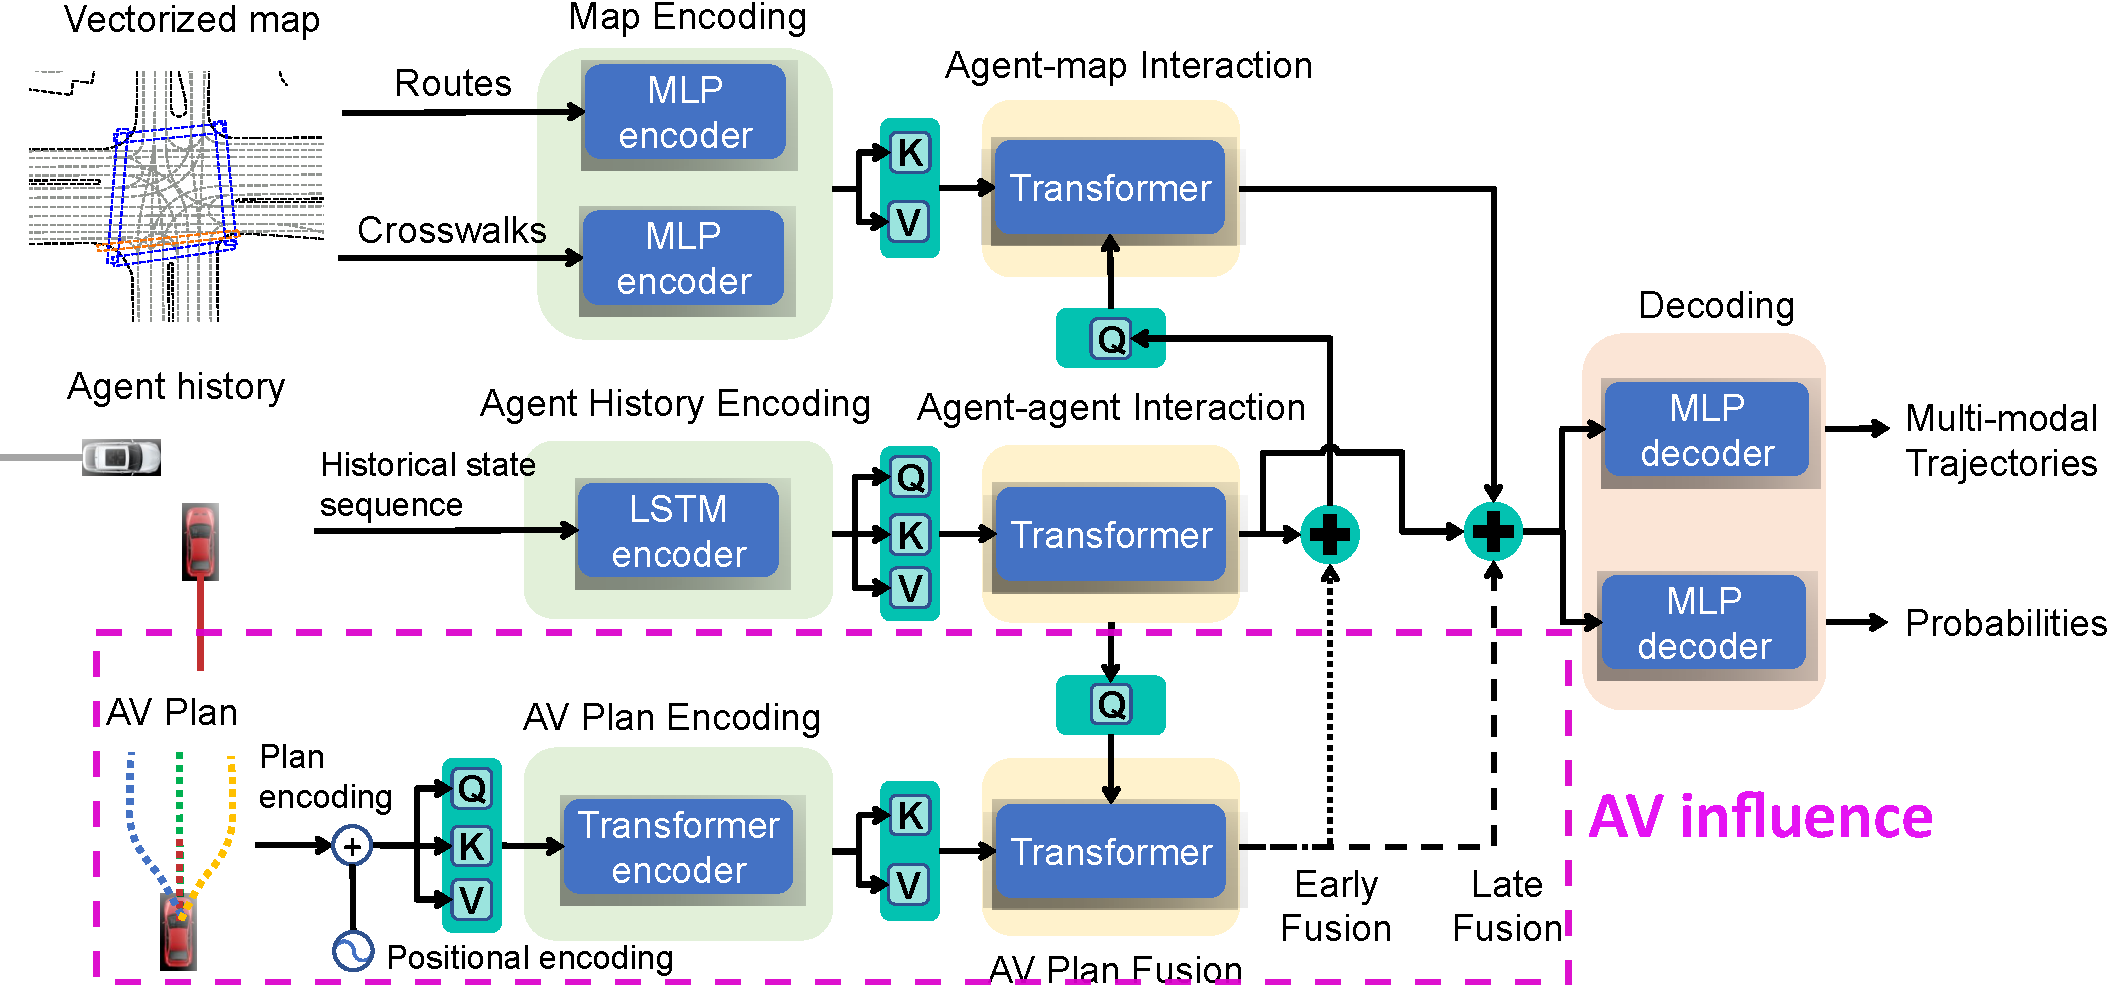
\includegraphics[width=0.8\linewidth]{2_cmp_vs_pmp.pdf}
	\caption{Example of a Conditional Motion Prediction (CMP) network. We \textcolor{magenta}highlight the influence of the \ac{AD} in the prediction of surrounding agents}
	Source: \textit{Conditional Predictive Behavior Planning with Inverse Reinforcement Learning for Human-like Autonomous Driving} \cite{huang2023conditional}
	\label{fig:2_cmp_vs_pmp}
\end{figure}

Nevertheless, to ensure safety under various predicted trajectories of the surrounding agents, our \ac{ADS} must overly conservative with inefficient maneuvers, specifically in arbitrarily complex traffic scenarios, because passive \ac{MP} models ignore the fact that the future states of an agent can influence the future actions of other agents, what is the most realistic situation. To this end, researchers recently started to explore a more coherent interactive prediction and planning framework which relies on predicting the surrounding agents future trajectories conditioned on the ego-vehicle future actions \cite{tang2019multiple} \cite{rhinehart2019precog} \cite{khandelwal2020if}, as a preliminary state to implement a fully-interaction graph where the future states of all agents (either autonomous prototypes or human-driven) influence in the decision of all agents. Under such frameworks, the \acs{ADS} can reason over potential actions while considering its influence on surrounding agents, as observed in Figure \ref{fig:2_cmp_vs_pmp}, inducing less conservative and more efficient maneuvers in highly interactive scenarios. \cite{huang2023conditional} propose a learning-based behaviour planning framework that learns to predict conditional multi-agent future trajectories, evaluating decisions from real-world human data. Moreover, they propose a two-stage learning process where the prediction model is trained first conditioned on the \ac{ADS} future actions, and then used as an environment model in the learning of the cost function with maximum entropy Inverse Reinforcement Learning (IRL). \cite{tang2022interventional} argue that CMP-based models essentially learns the posterior distribution of future trajectories conditioned on the future states of the ego-vehicle, where this future trajectory is treated as an observation, whilst safe and realistic prediction models should build the \ac{MP} to approximate the future trajectory distribution under the intervention of enforcing the \ac{ADS} future states, referring this new task as Interventional Behaviour Prediction (IBP). As aforementioned, the algorithms developed throughout this thesis do not focus on the joint study of the prediction and behaviour planning modules, but on studying efficient and powerful PMP algorithms without considering the future states of the autonomous agents as an additional condition. \\

Once the difference between CMP and PMP is stated












Most traditional predictions methods \cite{huang2022survey}, which usually only consider physics-related factors (like the velocity and acceleration of the target vehicle that is going to be predicted) and road-related factors (prediction as close as possible to the road centerline), are only suitable for \textbf{short-time} prediction tasks \cite{huang2022survey} and simple traffic scenarios, such as constant velocity (CV) in a highway or a curve (Constant Turn Rate Velocity, CTRV) where a single path is allowed, i.e. multiple choices computation are not required. Recently, MP methods based on DL have become increasingly popular since they are able not only to take into account these above-mentioned factors but also consider interaction-related factors (like agent-agent \cite{gupta2018social}, agent-map \cite{casas2018intentnet} and map-map \cite{liang2020learning}) in such a way the algorithm can adapt to more complex traffic scenarios (intersections, sudden breaks and accelerations, etc.). It must be consider that multimodal, specially in the field of vehicle motion prediction, does not refer necessarily to different directions (e.g. turn to the left, turn to the right, continue forward in an intersection), but it may refer to different predictions in the same direction that model a sudden positive or negative acceleration, so as to imitate a realistic human behaviour in complex situations. As expected, neither classical nor Machine Learning (ML) methods can model these situations \cite{huang2022survey}.

\begin{table*}[t]
	\begin{center}
		\caption{Main state-of-the-art methods for Motion Prediction. Main categories are Encoder (splitted into motion history, social info (agent interactions) and map info (physical information)), Decoder, Output representation and Distribution over future trajectories.}
		%\begin{tabular}{| c | cccccc |}
		%\begin{tabular}{| c | cccccc |}
		\begin{tabular}{r |ccc|c|c|c}
			
			\toprule
			\textbf{Method}	&	& \textbf{Encoder}	&	& \textbf{Decoder}	& \textbf{Output}  & \textbf{Trajectory Distribution}	\\
			& Motion history	& Social info	& Map info	&	&	&	\\
			\midrule
			\midrule
			SocialLSTM~\cite{alahi2016social}	& LSTM	& spatial pooling	& --	& LSTM	& states	& samples	\\
			SocialGan~\cite{gupta2018social}	& LSTM	& maxpool	& --	& LSTM	& states	& samples	\\
			Jean~\cite{mercat2020multiattentmotion}	& LSTM	& attention	& --	& LSTM	& states	& GMM	\\
			TNT~\cite{zhao2020tnt}	& polyline	& maxpool, attention	& polyline	& MLP	& states	& weighted set	\\
			LaneGCN~\cite{liang2020learninggraph}	& 1D-conv	& GNN	& GNN	& MLP	& states	& weighted set	\\
			WIMP~\cite{khandelwal2020if}	& LSTM	& GNN+attention	& polyline	& LSTM	& states	& GMM	\\
			VectorNet~\cite{gao2020vectornet}	& polyline	& maxpool, attention	& polyline	& MLP	& states	& unimodal	\\
			SceneTransformer~\cite{ngiam2021scene}	& attention	& attention	& polyline	& attention	& states	& weighted set	\\
			HOME~\cite{gilles2021home}	& raster	& attention	& raster	& conv	& states	& heatmap	\\
			GOHOME~\cite{gilles2021gohome}	& 1D-conv+GRU	& GNN	& GNN	& MLP	& states	& heatmap	\\
			MP3~\cite{casas2021mp3}	& raster	& conv	& raster	& conv	& cost function	& weighted samples	\\
			%CoverNet~\cite{phan2019covernet}	& raster	& conv	& raster	& lookup	& states	& GMM w/ dynamic anchors	\\
			%DESIRE~\cite{lee2017desire}	& GRU	& spatial pooling	& raster	& GRU	& states	& samples	\\
			ExploringGAN~\cite{gomez2022exploring}	& LSTM	& attention	& polyline	& LSTM	& states	& unimodal	\\
			% MFP~\cite{tang2019multiple}	& GRU	& RNNs+attention	& raster	& GRU	& states	& samples	\\
			%MANTRA~\cite{marchetti2020mantra}	& GRU	& --	& raster	& GRU	& states	& samples	\\
			%PRANK~\cite{biktairov2020prank}	& raster	& conv	& raster	& lookup	& states	& weighted set	\\
			%IntentNet~\cite{casas2018intentnet}	& raster	& conv	& raster	& conv	& states	& unimodal	\\
			Multimodal~\cite{cui2019multimodal}	& raster	& conv	& raster	& conv	& states	& weighted set	\\
			MultiPath~\cite{chai2019multipath}	& raster	& conv	& raster	& MLP	& states	& GMM w/ static anchors	\\
			MultiPath++~\cite{varadarajan2021multipath++}	& LSTM	& RNNs+maxpool	& polyline	& MLP	& control poly	& GMM	\\
			%PLOP~\cite{buhet2021plop}	& LSTM	& conv	& raster	& MLP	& state poly	& GMM	\\
			Trajectron++\cite{salzmann2020trajectron++}	& LSTM	& RNNs+attention	& raster	& GRU	& controls	& GMM	\\
			CRAT-PRED\cite{schmidt2022crat}	& LSTM	& GNN+attention	& --	& MLP	& states	& weighted set	\\
			%R2P2~\cite{rhinehart2018r2p2}	& GRU	& --	& polyline	& GRU	& motion	& samples	\\
			%DKM~\cite{cui2020deep}	& raster	& conv	& raster	& conv	& controls	& weighted set	\\
			\midrule					
			\textbf{Ours - Social baseline}	& LSTM	& GNN+attention	& --	& LSTM	& states	& weighted samples	\\
			\textbf{Ours - Map baseline}	& LSTM	& GNN+attention	& polyline 	& LSTM	& states	& weighted samples	\\
			\bottomrule
		\end{tabular}
		\label{table:related_work}
	\end{center}
\end{table*} 

In order to classify DL based MP methods, we distinguish several important features: Motion history, Social information (agent interactions), Map information (road encoding), how the model returns the output trajectory and its corresponding distribution. Table \ref{table:related_work} summarizes several SOTA methods, inspired in the survey proposed by \cite{varadarajan2021multipath++}.

\begin{itemize}
	
	\item \textbf{Motion history}: Most methods encode the sequence of past observed states using 1D-convolution \cite{liang2020learninggraph} \cite{mercat2020multiattentmotion}, able to model spatial information, or via a recurrent net \cite{gomez2022exploring} \cite{alahi2016social} (LSTM, GRU), which are more useful to handle temporal information. Other methods that use a raster version of the whole scenario represent the agent states rendered as a stack of binary mask images depicting agent oriented bounding boxes \cite{gilles2021home}. On the other hand, other approaches encode the past history of the agents in a similar way to the road components of the scene given a set of vectors or polylines \cite{zhao2020tnt, gao2020vectornet} that can model the high-order interactions among all components, or even employing attention to combine features across road elements and agent interactions \cite{ngiam2021scene}.
	
	\item \textbf{Social information}: In complex scenarios, motion history encoding of a particular target agent is not sufficient to represent the latent space of the traffic situation, but the algorithm must deal with a dynamic set of neighbouring agents around the target agent. Common techniques are aggregating neighbour motion history with a permutation-invariant set operator: soft attention \cite{ngiam2021scene, gomez2022exploring}, a combination of soft attention and RNN \cite{varadarajan2021multipath++} / GNN \cite{schmidt2022crat} or social pooling \cite{alahi2016social, gupta2018sgan}. Raster based approaches rely on 2D convolutions \cite{chai2019multipath} \cite{casas2021mp3} over the spatial grid to implicitly capture agent interactions in such a way long-term interactions are dependent on the neural network receptive fields.
	
	%quito la cita suelta \cite{murciego2018topological} para evitar self-citations en review y ahorrar 4 lineas. En el CR la puedes añadir.
	
	\item \textbf{Map information}: High-fidelity maps~\cite{can2022maps} have been widely adopted to provide offline information (also known as physical context) to complement the online information provided by the sensor suite of the vehicle and its corresponding algorithms. Recent learning-based approaches \cite{mahjourian2022occupancy, casas2018intentnet, ivanovic2021heterogeneous}, which present the benefit of having probabilistic interpretations of different behaviour hypotheses, require to build a representation to encode the trajectory and map information. Map information is probably the feature with the clearest dichotomy: raster vs vector treatment. The raster approach encodes the world around the particular target agent as a stack of images (generally from a top-down orthographic view, also known as Bird's Eye View). This world encoding may include from agent state history, agent interactions and usually the road configuration, integrated all this different-sources information as a multi-channel image \cite{gilles2021home}, in such a way the user can use an off-the-shelf Convolutional Neural Network (CNN) based pipeline in order to leverage this powerful information. Nevertheless, this representation has several downsides: constrained field of view, difficulty in modeling long-range interactions and even difficulty in representing continuous physical states due to the inherent world to image (pixel) discretization. On the other hand, the polyline approach may describe curves, such as lanes, boundaries, intersections and crosswalks, as piecewise linear segments, which usually represents a more compact and efficient representation than using CNNs due to the sparse nature of road networks. Some state-of-the-art algorithms not only describe the world around a particular agent as a set-of-polylines \cite{khandelwal2020if} \cite{zhao2020tnt} in an agent-centric coordinate system, but they also leverage the road network connectivity structure \cite{liang2020learninggraph} \cite{zeng2021lanercnn} treating road lanes as a set of nodes (waypoints) and edges (connections between waypoints) in a graph neural network so as to include the topological and semantic information of the map.
	
	% Additional bio: deo2018cstlstmpool, rhinehart2019precog
	
	\item \textbf{Decoder}: Pioneering works of DL based MP usually adopt the autoencoder architecture, where the decoder is often represented by a recurrent network (GRU, LSTM, etc., specially designed to handle temporal information) to generate future trajectories in an autoregressive way, or by CNNs \cite{gilles2021home} \cite{gilles2021gohome} / MLP \cite{liang2020learninggraph} \cite{schmidt2022crat} using the non-autoregressive strategy. The method may use an autoregressive strategy where the pipeline generates tokens (in this case, positions or relative displacements) in a sequential manner, in such a way the new output is dependent on the previously generated output, whilst MLP \cite{schmidt2022crat}, CNN \cite{gilles2021home} or transformer \cite{ngiam2021scene} based strategies usually follow a non-autoregressive strategy, where from a latent space the whole future trajectory is predicted.
	
	\item \textbf{Output}: The most popular model output representation is a sequence of states (absolute positions) or state differences (relative displacements for any dimension considered). The spacetime trajectory may be intrinsically represented as a continous polynomial representation or a sequence of sample points. Other works \cite{gilles2021home} \cite{gilles2021gohome} first predict a heatmap and then decode the corresponding output trajectories after sampling points from the heatmap, whilst \cite{casas2021mp3} \cite{zeng2019end} learn a cost function evaluator of trajectories that are enumerated heuristically instead of being generated by a learned model. 
	
	\item \textbf{Trajectory Distribution}: The choice of output trajectory distributions has several approaches on downstream applications. Regardless the agent to be predicted is described as a (non-)holonomic \cite{triggs1993motion} platform, an intrinsic property of the motion prediction problem is that the agent must follow one of a diverse set of possible future trajectories. A popular choice to represent a multimodal prediction are Gaussian Mixture Models (GMMs) due to their compact parameterized form, where mode collapse (associated frequently to GMMs) is addressed through the use of trajectory anchors \cite{chai2019multipath} or training  tricks \cite{cui2019multimodal}. Other approaches model a discrete distribution via a collection of trajectory samples extracted from a latent space and decoded by the model \cite{rhinehart2018r2p2} or over a set of trajectories (fixed or a priori learned) \cite{liang2020learninggraph}.
	
	% Additional bio: \cite{biktairov2020prank}
	
\end{itemize}

After classifying main SOTA methods, we conclude this section presenting the main characteristics of our baseline approaches. We make use of LSTM to encode the past motion history, GNN in combination with soft-attention the compute social interactions, a set-of-polylines to represent the most important map information and LSTM to decode the trajectories from the latent space. The output multimodal prediction is represented by a set of states with their corresponding confidences indicating the most plausible modes.
% Social LSTM \cite{alahi2016social} applies an LSTM autoencoder (adopting the NLL loss to model the error for each future step) whilst its generative continuation, Social GAN \cite{gupta2018social} uses an adversarial \cite{goodfellow2014gan} frame with social attention encoding the input trajectories with LSTM and then decoding different multiple modalities with the inherent noise associated to generative models, adopting per-step MSE loss. DESIRE \cite{lee2017desire} applies a conditional variational autoencoder in order to sample a diverse set of plausible modalities, making use of a GRU to generate the final predictions. 

% Moreover, SoPhie \cite{sadeghian2019sophie} represents one of the first DL based MP models that leverages two sources of information: the path states (position, velocity, heading, etc.) of all the agents in the scene and the physical context information, using Bird's Eye View (BEV) images as inputs and CNN as feature extractor. After fusing both physical and social attention, this model can successfully predict multiple acceptable trajectories that respect both social constraints (not collide with other agents) and physical constraints (most predictions are in the plausible area). Authors show that by modeling jointly the information about the physical environment and interactions between all agents, the model is able to learn better than when both sources of information are used independently

% In that sense, high-fidelity maps~\cite{can2022maps} have been widely adopted to provide offline information (also known as physical context) to complement the online information provided by the sensor suite of the vehicle and its corresponding algorithms. Recent learning-based approaches \cite{mahjourian2022occupancy, xiao2022multimodalend2end, casas2018intentnet, deo2018cstlstmpool, rhinehart2019precog, ivanovic2021heterogeneous}, which present the benefit of having probabilistic interpretations of different behaviour hypotheses, require to build a representation to encode the trajectory and map information. Hong et al.~\cite{hong2019rules} assumes that detections around the vehicle are provided and focuses on behaviour prediction by encoding entity interactions with ConvNets. \textbf{Intentnet}~\cite{casas2018intentnet} proposes to jointly detect traffic participants (mostly focused on vehicles) and predict their trajectories using raw LiDAR pointcloud and HD map information. %PRECOG~\cite{rhinehart2019precog} aims to capture the future stochasticity by flow-based generative models. 
%
% \textbf{MultiPath} by Chai et al.~\cite{chai2019multipath} uses ConvNets as encoder and adopts pre-defined trajectory anchors to regress multiple possible future trajectories.

% \textbf{HOME} by Gilles et al.~\cite{gilles2021home} presented a novel representation for multimodal trajectory prediction, where the model takes as input the context (map) and history of past trajectories, and generates an unconstrained 2D heatmap representation of the agent’s possible future trajectories, which represents the probability distribution of the agent’s future location. The method builds on simple architecture with classic convolution networks coupled with attention mechanism for agent interactions. Fig.~\ref{fig:prev_models} shows the SoPhie and HOME architectures. Both methods have two-streams, one for each input (trajectories and map), and use CNNs to process the map or physical context.

% In Section~\ref{sec:ours} we explain our solution to this trade-off problem.

\

\section{Introduction}
\label{sec:2_introduction}

\begin{figure}[h]
	\centering
	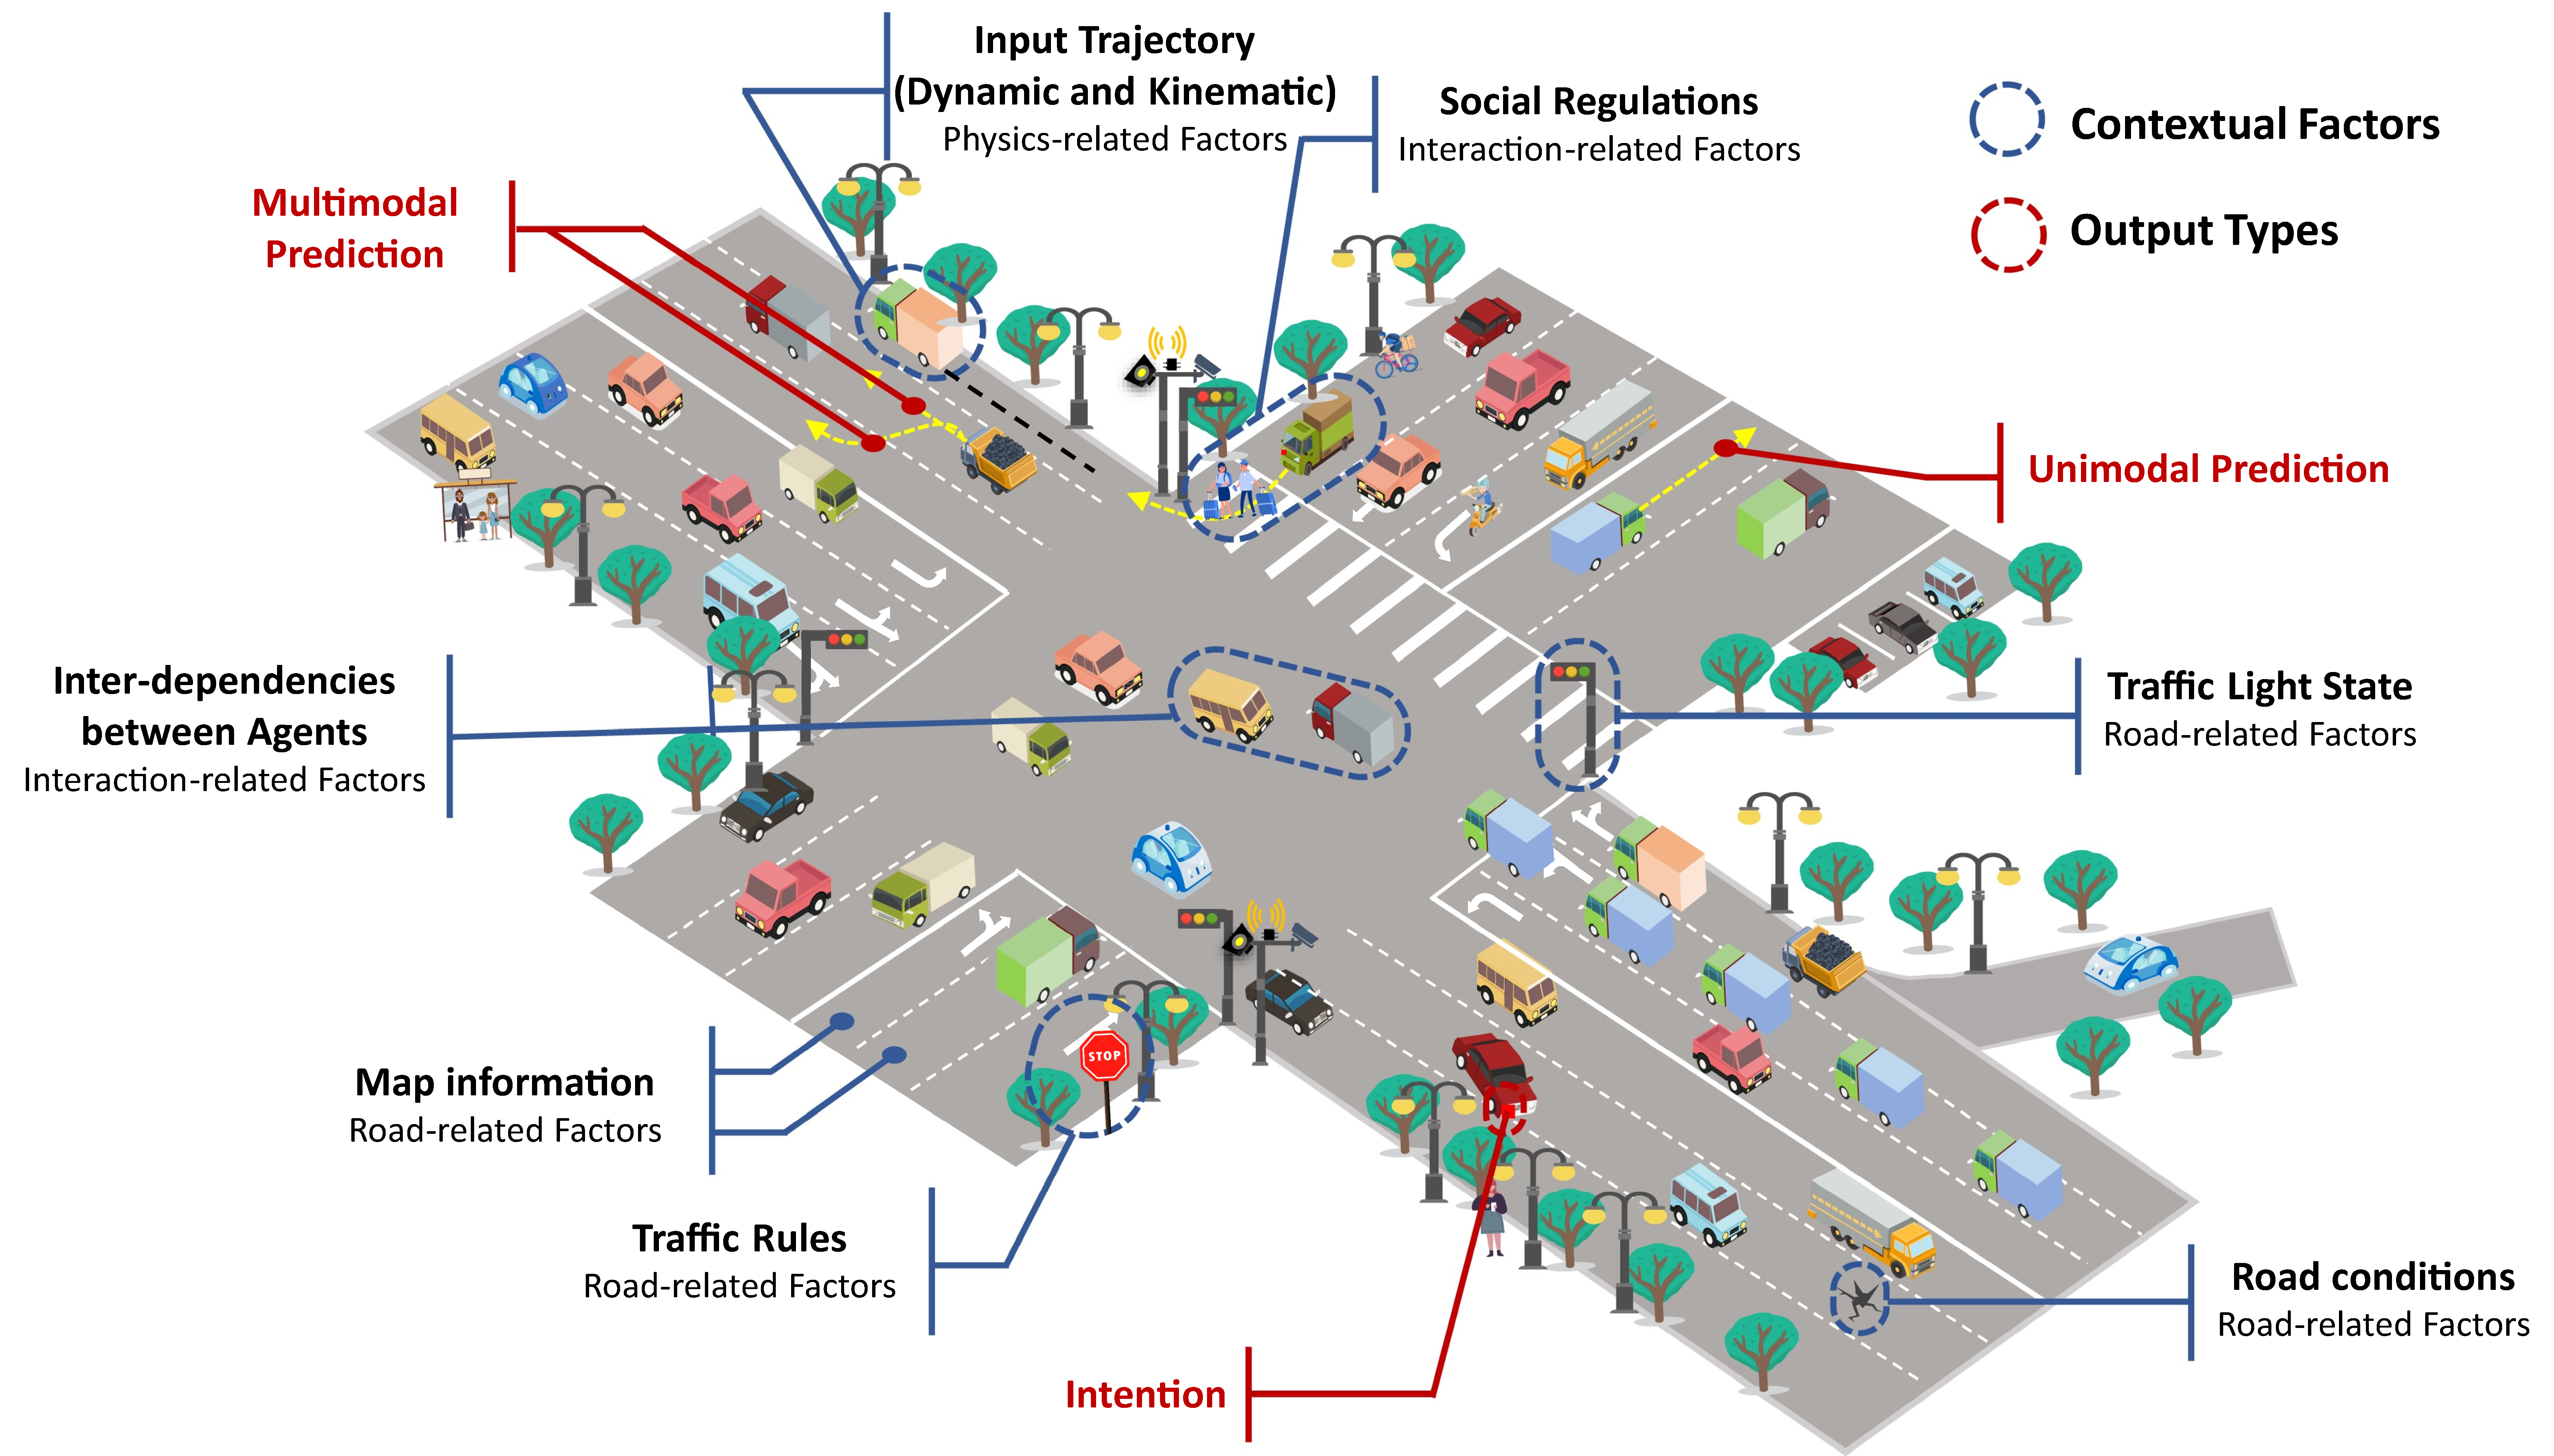
\includegraphics[width=\linewidth]{2_inputs_outputs_mp.pdf}
	\caption{Contextual factors and output types in Vehicle Motion Prediction}
	%Source: \textit{A survey on trajectory-prediction methods for autonomous driving} \cite{huang2022survey}
	\label{fig:2_input_output_map}
\end{figure}



\section{Problem Formulation of Motion Prediction}
\label{sec:2_problem_formulation_mp}

Given a sequence of past trajectories $a_{P}=[a_{-T^{'}+1},a_{-T^{'}+2},...,a_{0}]$ for an agent, we aim to predict its future steps $a_{F}=[a_{1},a_{2},...,a_{T}]$ up to a fixed time step $T$. Running in a specific traffic scenario, each actor will interact with static HD maps $m$ and the other dynamic actors, meeting the corresponding traffic and social rules. Therefore, the probabilistic distribution that we want to capture is $p(a_F|m, a_P, a^O_P)$, where $a^O_P$ denotes the other actors' observed states. 




The output of our model is $A_F = \{a_{F}^k\}_{k \in [0,K-1]}= \{(a_{1}^k,a_{2}^k,...,a_{T}^k)\}_{k \in [0,K-1]}$ for each actor, while motion forecasting tasks and subsequent decision modules usually expect us to output a set of trajectories. 
%
TNT \cite{zhao2020tnt}-like methods' distribution can be approximated as
\begin{equation}
	\sum_{\tau \in T(m, a_P, a^O_P)}{p(\tau|m, a_P, a^O_P)p(a_F|\tau, m, a_P, a^O_P)}
\end{equation}
where $T(m, a_P, a^O_P)$ is the space of candidate goals depending on the driving context.
However, the map space $m$ is large, and the goal space $T(m, a_P, a^O_P)$ requires careful design. In that sense, some methods expect to accurately predict the actor motion by extracting good features. For example, LaneGCN~\cite{liang2020learninggraph} tries to approximate $p(a_F|m, a_P, a^O_P)$ by modeling $p(a_F|M_{a_0}, a_P, a^O_P)$, where $M_{a_0}$ is a "local" map features that is related to the actor state $a_0$ at final observed step $t=0$. To extract $M_{a_0}$, they use $a_0$ as an anchor to retrieve its surrounding map elements and aggregate their features. As stated by \cite{wang2022ganet}, computing the local map information is only a part of the solution, but also proposing preliminary guidance for the model in a heuristic way, as well as calculating the goal area maps information using DL, may be of great importance for accuracy trajectory prediction. Then, our future probability distribution is enhanced by these preliminary preprocessed proposals and predicted goals as anchors to explicitly aggregate their surrounding map features as goal areas. 

\section{Physic-based Motion Prediction}
\label{sec:2_physic_based_mp}

\section{Deep Learning based Motion Prediction}
\label{sec:2_dl_based_mp}

\section{Vehicle Motion Prediction}
\label{sec:2_vehicle_based_mp}
%%%%%%%%%%%%%%%%%%%%%%%%%%%%%%%%%%%%%%%%%%%%%%%%%%%%%%%%%%%%%%%%%%%%%%%%%%% 
% 
% Generic template for TFC/TFM/TFG/Tesis
% 
% By:
% + Javier Macías-Guarasa. 
% Departamento de Electrónica
% Universidad de Alcalá
% + Roberto Barra-Chicote. 
% Departamento de Ingeniería Electrónica
% Universidad Politécnica de Madrid   
% 
% Based on original sources by Roberto Barra, Manuel Ocaña, Jesús Nuevo,
% Pedro Revenga, Fernando Herránz and Noelia Hernández. Thanks a lot to
% all of them, and to the many anonymous contributors found (thanks to
% google) that provided help in setting all this up.
% 
% See also the additionalContributors.txt file to check the name of
% additional contributors to this work.
% 
% If you think you can add pieces of relevant/useful examples,
% improvements, please contact us at (macias@depeca.uah.es)
% 
% You can freely use this template and please contribute with
% comments or suggestions!!!
% 
%%%%%%%%%%%%%%%%%%%%%%%%%%%%%%%%%%%%%%%%%%%%%%%%%%%%%%%%%%%%%%%%%%%%%%%%%%% 

\chapter{Theoretical Background}
\label{cha:theoretical_background}

\begin{FraseCelebre}
	\begin{Frase}
		Desde que el mundo cambió, \\
		estamos mucho más unidos con los Digimon, \\
		luchamos juntos contra el mal. \\ 

		Algo extraño pasaba, \\
		Digievolucionaban, en tamaño y color, \\
		Ellos son los Digimon. \\
	\end{Frase}
	\begin{Fuente}
		Opening 1 de Digimon: "Butterfly" \\
		Autor original: Kōji Wada
	\end{Fuente}
\end{FraseCelebre}

\section{Introduction}
\label{sec:3_introduction}

As commented in previous sections, the \ac{MP} algorithms covered by this thesis range from tracking multiple objects and subsequent prediction with physics-based methods to the most recent \ac{SOTA} techniques to compute the deep traffic context and then decode multimodal predictions with associated confidences, assuming the physical information is given and surrounding participants have been multi-tracked beforehand. Throughout this Chapter, an in-depth theoretical study will be made of those algorithms, neural networks or heuristics that form a direct part of the development of this work in order to address the proposed methods in future chapters.

First of all, we will start with the mathematical formulation of the methods to perform physics-based Multi-Object Tracking, from the well-known techniques Kalman Filter \cite{kalman1960new} for the agents states estimation to the Hungarian algorithm \cite{kuhn1955hungarian} for the association of detections and trackers, which represents the preliminary stage before carrying out the subsequent prediction. On top of that, since several single-trajectory models (\ac{CTRV}, \ac{CTRA}) are used to compute the most plausible centerlines in the Argoverse 1 \cite{chang2019argoverse} and Argoverse 2 \cite{wilson2023argoverse}, we will review the state transition equations to properly understand the constraints for each model. Furthermore, the principal \ac{DL} techniques (e.g. 1D-CNN, LSTM, GCN, Attention mechanisms) and training losses used in this work to encode and decode the aimed multimodal will be stated, first a general mathematical formulation and applications and then how the corresponding technique is used in the \ac{MP} field.

\section{Physics-based algorithms}
\label{sec:3_pb_formulation}

% https://arxiv.org/pdf/1710.04055.pdf
% https://github.com/NickNair/Multiple-Object-Tracking-using-Kalman-Filter

As stated in Chapter \ref{cha:related_works} Section \ref{sec:2_introduction}, initially researchers rely on physics-based methods which are basic and straightforward. These methods may not offer high accuracy, but many models use the underlying idea of physics-based models to improve their accuracy. Physics-based approaches yield better results when the movement of vehicles is described by kinematics or dynamics models accurately. Nevertheless, the physical model of traffic participants is constantly evolving, so most physics-based models are only applicable for short-term predictions of no more than one second. In this Section we will study the mathematical formulation of the physics-based prediction algorithms, as well as the data association problem regarding the Multi-Object Tracking stage, that are directly related to our algorithm proposed in Chapter \ref{cha:smartmot_exploiting_the_fusion_of_hdmaps_and_mot}.

\subsection{Kalman Filter under the hood}
\label{subsec:3_kf_formulation}

The Kalman Filter \cite{kalman1960new} is a recursive algorithm used for estimating the state of a dynamic system in the presence of noise. It is widely used in various fields such as engineering, control systems, and robotics. The algorithm works by combining a prediction of the system state based on a mathematical model with measurements (updates) from sensors to improve the accuracy of the state estimation, as shown in Figure \ref{fig:chapter_3_theoretical_background/KF_cycle}. The Kalman Filter is a powerful algorithm for state estimation, and it has many variations and extensions that can handle various types of systems and measurements. The filter can be applied to non-linear systems using the Extended Kalman Filter or the Unscented Kalman Filter, and it can handle multiple models using the multiple model Kalman Filter. The filter can also be used for smoothing, which involves estimating the state of the system based on past and future measurements.

\begin{figure}[h]
	\centering
	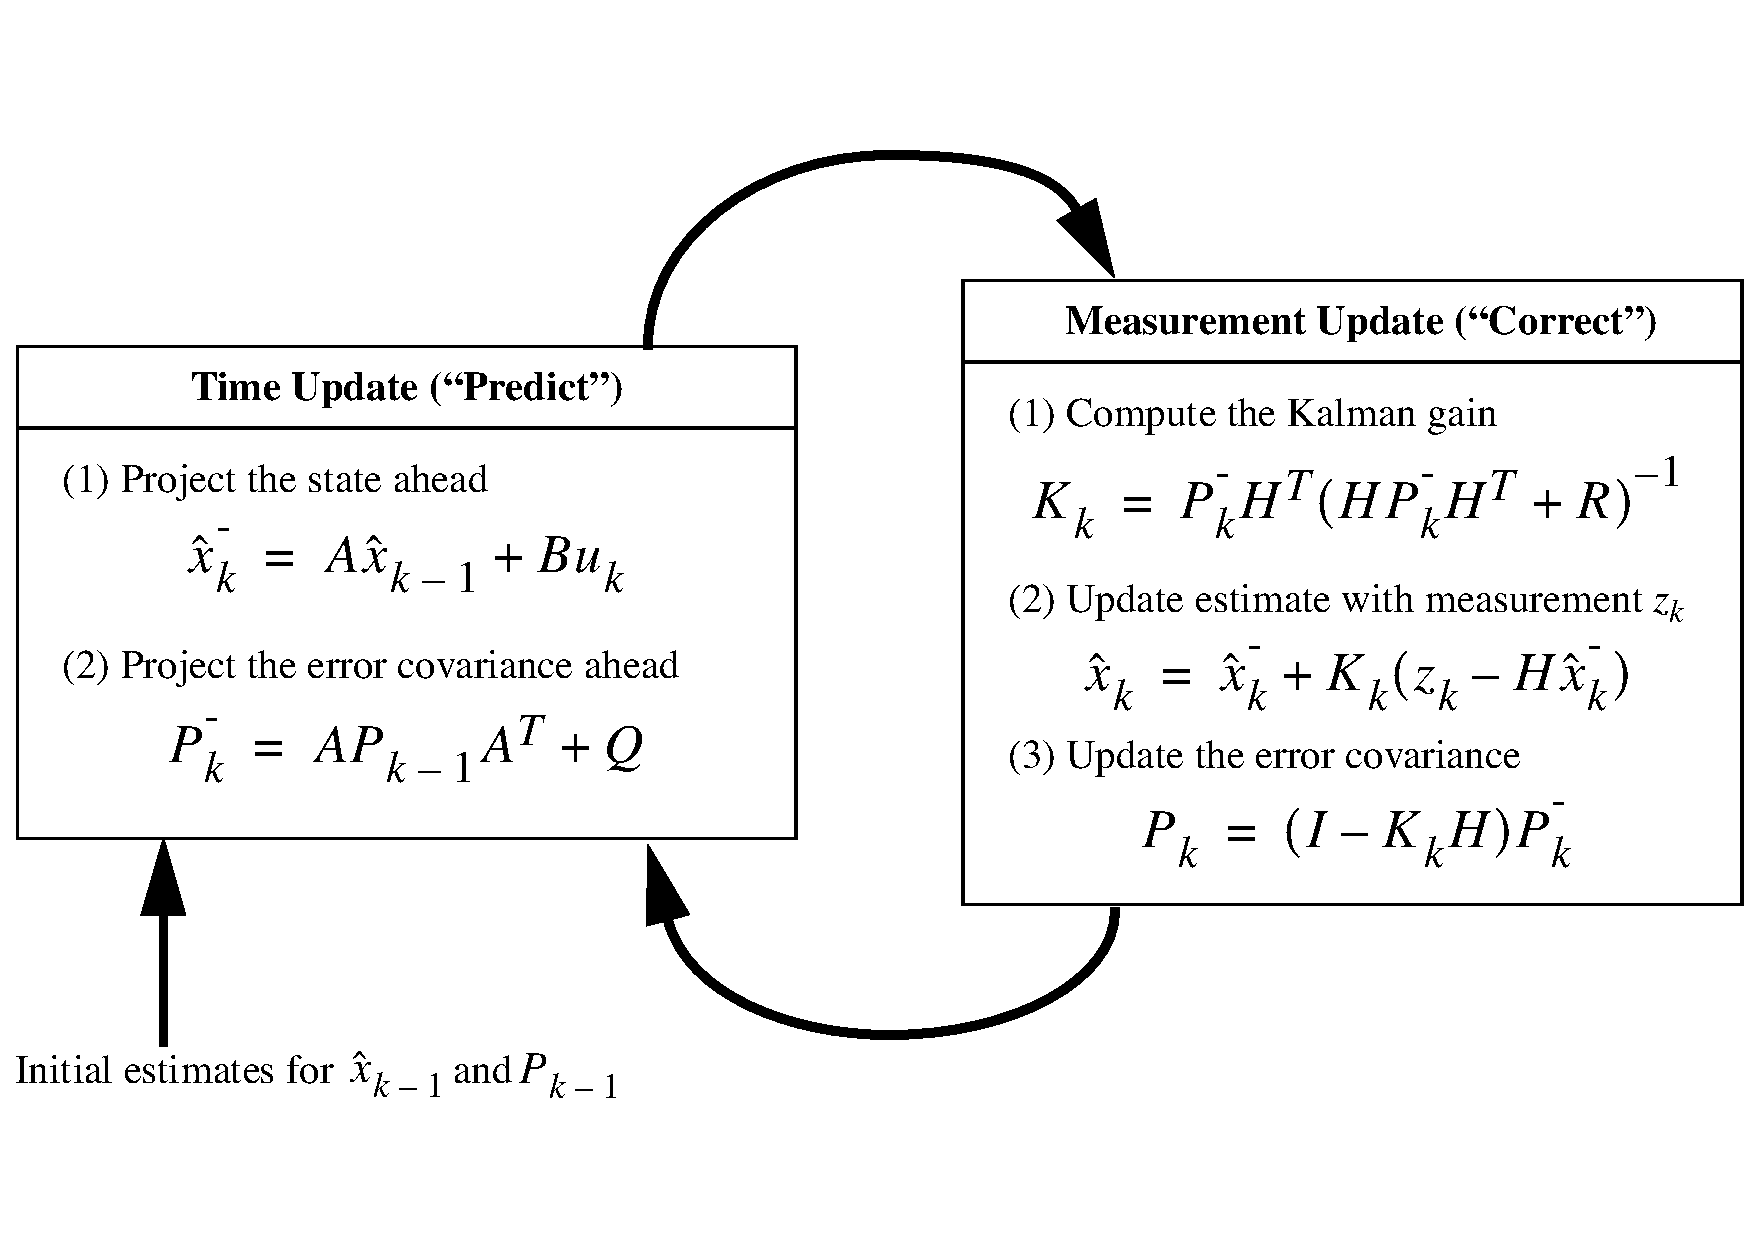
\includegraphics[width=\linewidth]{chapter_3_theoretical_background/KF_cycle.pdf}
	\caption[Overview of the Kalman Filter Predict-Update cycle]{Overview of the Kalman Filter Predict-Update cycle. The Kalman filter keeps track of the estimated state of the system and the variance or uncertainty of the estimate. The estimate is updated using a state transition model and measurements}
	Source: \textit{An introduction to the kalman filter} \cite{bishop2001introduction}
	\label{fig:chapter_3_theoretical_background/KF_cycle}
\end{figure}

In its most simple version, the Kalman filter assumes that the system can be described using a set of linear equations, where the state of the system can be represented by a vector $\mathbf{x}_k$, and the measurements can be represented by a vector $\mathbf{z}_k$. The Kalman filter also assumes that the noise in the system follows a Gaussian distribution.

The state estimation process is performed in two steps: the prediction step and the update step. In the prediction step, the current state of the system is predicted based on the previous state and a mathematical model of the system. In the update step, the predicted state is corrected based on a measurement from a sensor.

The prediction step can be represented using the following equations:

\begin{equation}
\begin{split}
	\hat{\mathbf{x}}_k^- = \mathbf{A} \hat{\mathbf{x}}_{k-1} + \mathbf{B} \mathbf{u}_k \\
	\mathbf{P}_k^- = \mathbf{A} \mathbf{P}_{k-1} \mathbf{A}^T + \mathbf{Q}
\end{split}
\end{equation}

where $\hat{\mathbf{x}}_k^-$ is the predicted state of the system at time $k$, $\hat{\mathbf{x}}_{k-1}$ is the estimated state of the system at time $k-1$, $\mathbf{A}$ is the state transition matrix, $\mathbf{B}$ is the control-input matrix, $\mathbf{u}_k$ is the control input at time $k$, $\mathbf{P}_k^-$ is the predicted error covariance matrix, and $\mathbf{Q}$ is the process noise covariance matrix. Note that the state transition, control-input and process noise covariance matrix values do not depend on the timestep time $k$.

On the other hand, the update step can be represented using the following equations:

\begin{equation}
	\begin{split}
		\mathbf{K}_k = \mathbf{P}_k^- \mathbf{H}_k^T (\mathbf{H} \mathbf{P}_k^- \mathbf{H}^T + \mathbf{R})^{-1} \\
		\hat{\mathbf{x}}_k = \hat{\mathbf{x}}_k^- + \mathbf{K}_k (\mathbf{z}_k - \mathbf{H}_k \hat{\mathbf{x}}_k^-) \\
		\mathbf{P}_k = (\mathbf{I} - \mathbf{K}_k \mathbf{H}) \mathbf{P}_k^-
	\end{split}
\end{equation}

where $\mathbf{K}_k$ is the Kalman gain, $\mathbf{H}$ is the measurement matrix, $\mathbf{R}_k$ is the measurement noise covariance matrix and $\mathbf{I}$ the identity matrix of the corresponding dimension. The Kalman gain determines the relative weight given to the predicted state and the measurement, and is adjusted based on the measurement noise covariance matrix. The measurement matrix relates the measurements to the state variables, and is used to convert the measurements into the same units as the state variables.

\subsection{Hungarian algorithm formulation}
\label{subsec:3_HA_formulation}

The Hungarian algorithm \cite{kuhn1955hungarian}, also known as the Munkres algorithm or the Kuhn-Munkres algorithm, is an efficient algorithm for solving the assignment problem in combinatorial optimization. The main concept behind this algorithm is an assignment problem that involves finding the optimal assignment of $n$ workers to $n$ jobs, given the cost of assigning each worker to each job.

The Hungarian algorithm works by iteratively finding a set of independent zero-cost assignments, which correspond to a perfect matching in a bipartite graph. These assignments are then used to reduce the problem size and find a new set of independent zero-cost assignments, until all workers are assigned to jobs.

The Hungarian algorithm has a time complexity of O($n^3$), which makes it one of the most efficient algorithms for solving the assignment problem. In this algorithm, the cost matrix C is assumed to be an $n \times n$ matrix, where each element $C_{i,j}$ represents the cost of assigning worker i to job j. The matrix M represents the matching, where each element $M_{i,j}$ is 1 if worker i is assigned to job j, and 0 otherwise.

\begin{algorithm}[]
	\SetAlgoLined
	\DontPrintSemicolon
	\SetKwInOut{Input}{Input}
	\SetKwInOut{Output}{Output}
	\Input{A cost matrix $C$ of size $n\times n$}
	\Output{A minimum cost perfect matching}
	Initialize the label vectors $u_i = \min_{j\in{1,\dots,n}} C_{i,j}$ and $v_j=0$ for all $i,j$;
	Initialize the empty matching $M$;
	\While{$|M| < n$}{
		Choose an unmatched row $i$;
		Initialize the set $T = {i}$ and the predecessor vector $P = \emptyset$;
		\While{true}{
			Let $S$ be the set of columns $j$ such that $i\in T$ and $C_{i,j} = u_i + v_j$;
			If $|S| > 0$, choose any column $j$ in $S$;
			\Else{
				Choose a column $j$ such that $v_j = \min_{k\in{1,\dots,n}} v_k$ and let $S$ be the set of rows $i$ such that $j\in M$ or $C_{i,j} = u_i + v_j$;
				Increment each $u_i$ for $i\in T$ by $\delta = \min_{i\in T,j\in S} (u_i+v_j-C_{i,j})$;
				Decrement each $v_j$ for $j\in S$ by $\delta$;
				\For{each row $i\in T$ and each column $j\in S$}{
					\If{$C_{i,j} = u_i+v_j$}{
						Add the edge $(i,j)$ to the alternating tree represented by $M$ and $P$;
						\If{$j$ is unmatched}{
							Augment $M$ along the alternating tree to create a larger matching;
							\Return the updated matching $M$;
						}
						\Else{
							Add $j$ to $T$ and continue the while loop;
						}
					}
				}
			}
		}
	}
	\caption{The Hungarian algorithm for solving the minimum cost perfect matching problem}
	\label{alg:3_ha}
\end{algorithm}

As observed in Algorithm \ref{alg:3_ha}, the Hungarian algorithm iteratively finds an uncovered zero in the cost matrix C and adds it to the matching M, while also adjusting the cost matrix to ensure that all rows and columns are covered by the matching. This is done by finding the minimum uncovered cost in each row and subtracting it from all uncovered costs in the row, and finding the minimum cost in each uncovered column and adding it to all uncovered costs in the column. Once all rows and columns are covered, the algorithm returns the final matching $M$.

In conclusion, the Hungarian algorithm is a powerful optimization algorithm that solves the assignment problem in polynomial time. The algorithm has a wide range of applications and can be easily adapted to handle various constraints and objectives. The algorithm is also guaranteed to find the optimal solution to the assignment problem, which makes it a valuable tool in many practical settings.
	
\subsection{State Transition Equations of Single-Trajectory Models}
\label{subsec:3_state_transitions_single_traj}

As stated in Chapter \ref{cha:related_works} Section \ref{subsubsec:2_single_trajectory_mp}, Single-trajectory prediction methods are used in the field of motion estimation and control, to predict the future state of an object based on its current state and motion. In these methods, the agents are mostly assumed to comply with motion models that describe their dynamic behavior in such a way these are not able to consider the road-related factors and the uncertainty of the current state is unreliable for long-term prediction. Then, these models should only be used for estimating unimodal trajectories of the surrounding agents in the short-term (no more than 1-s).

\begin{figure}[h]
	\centering
	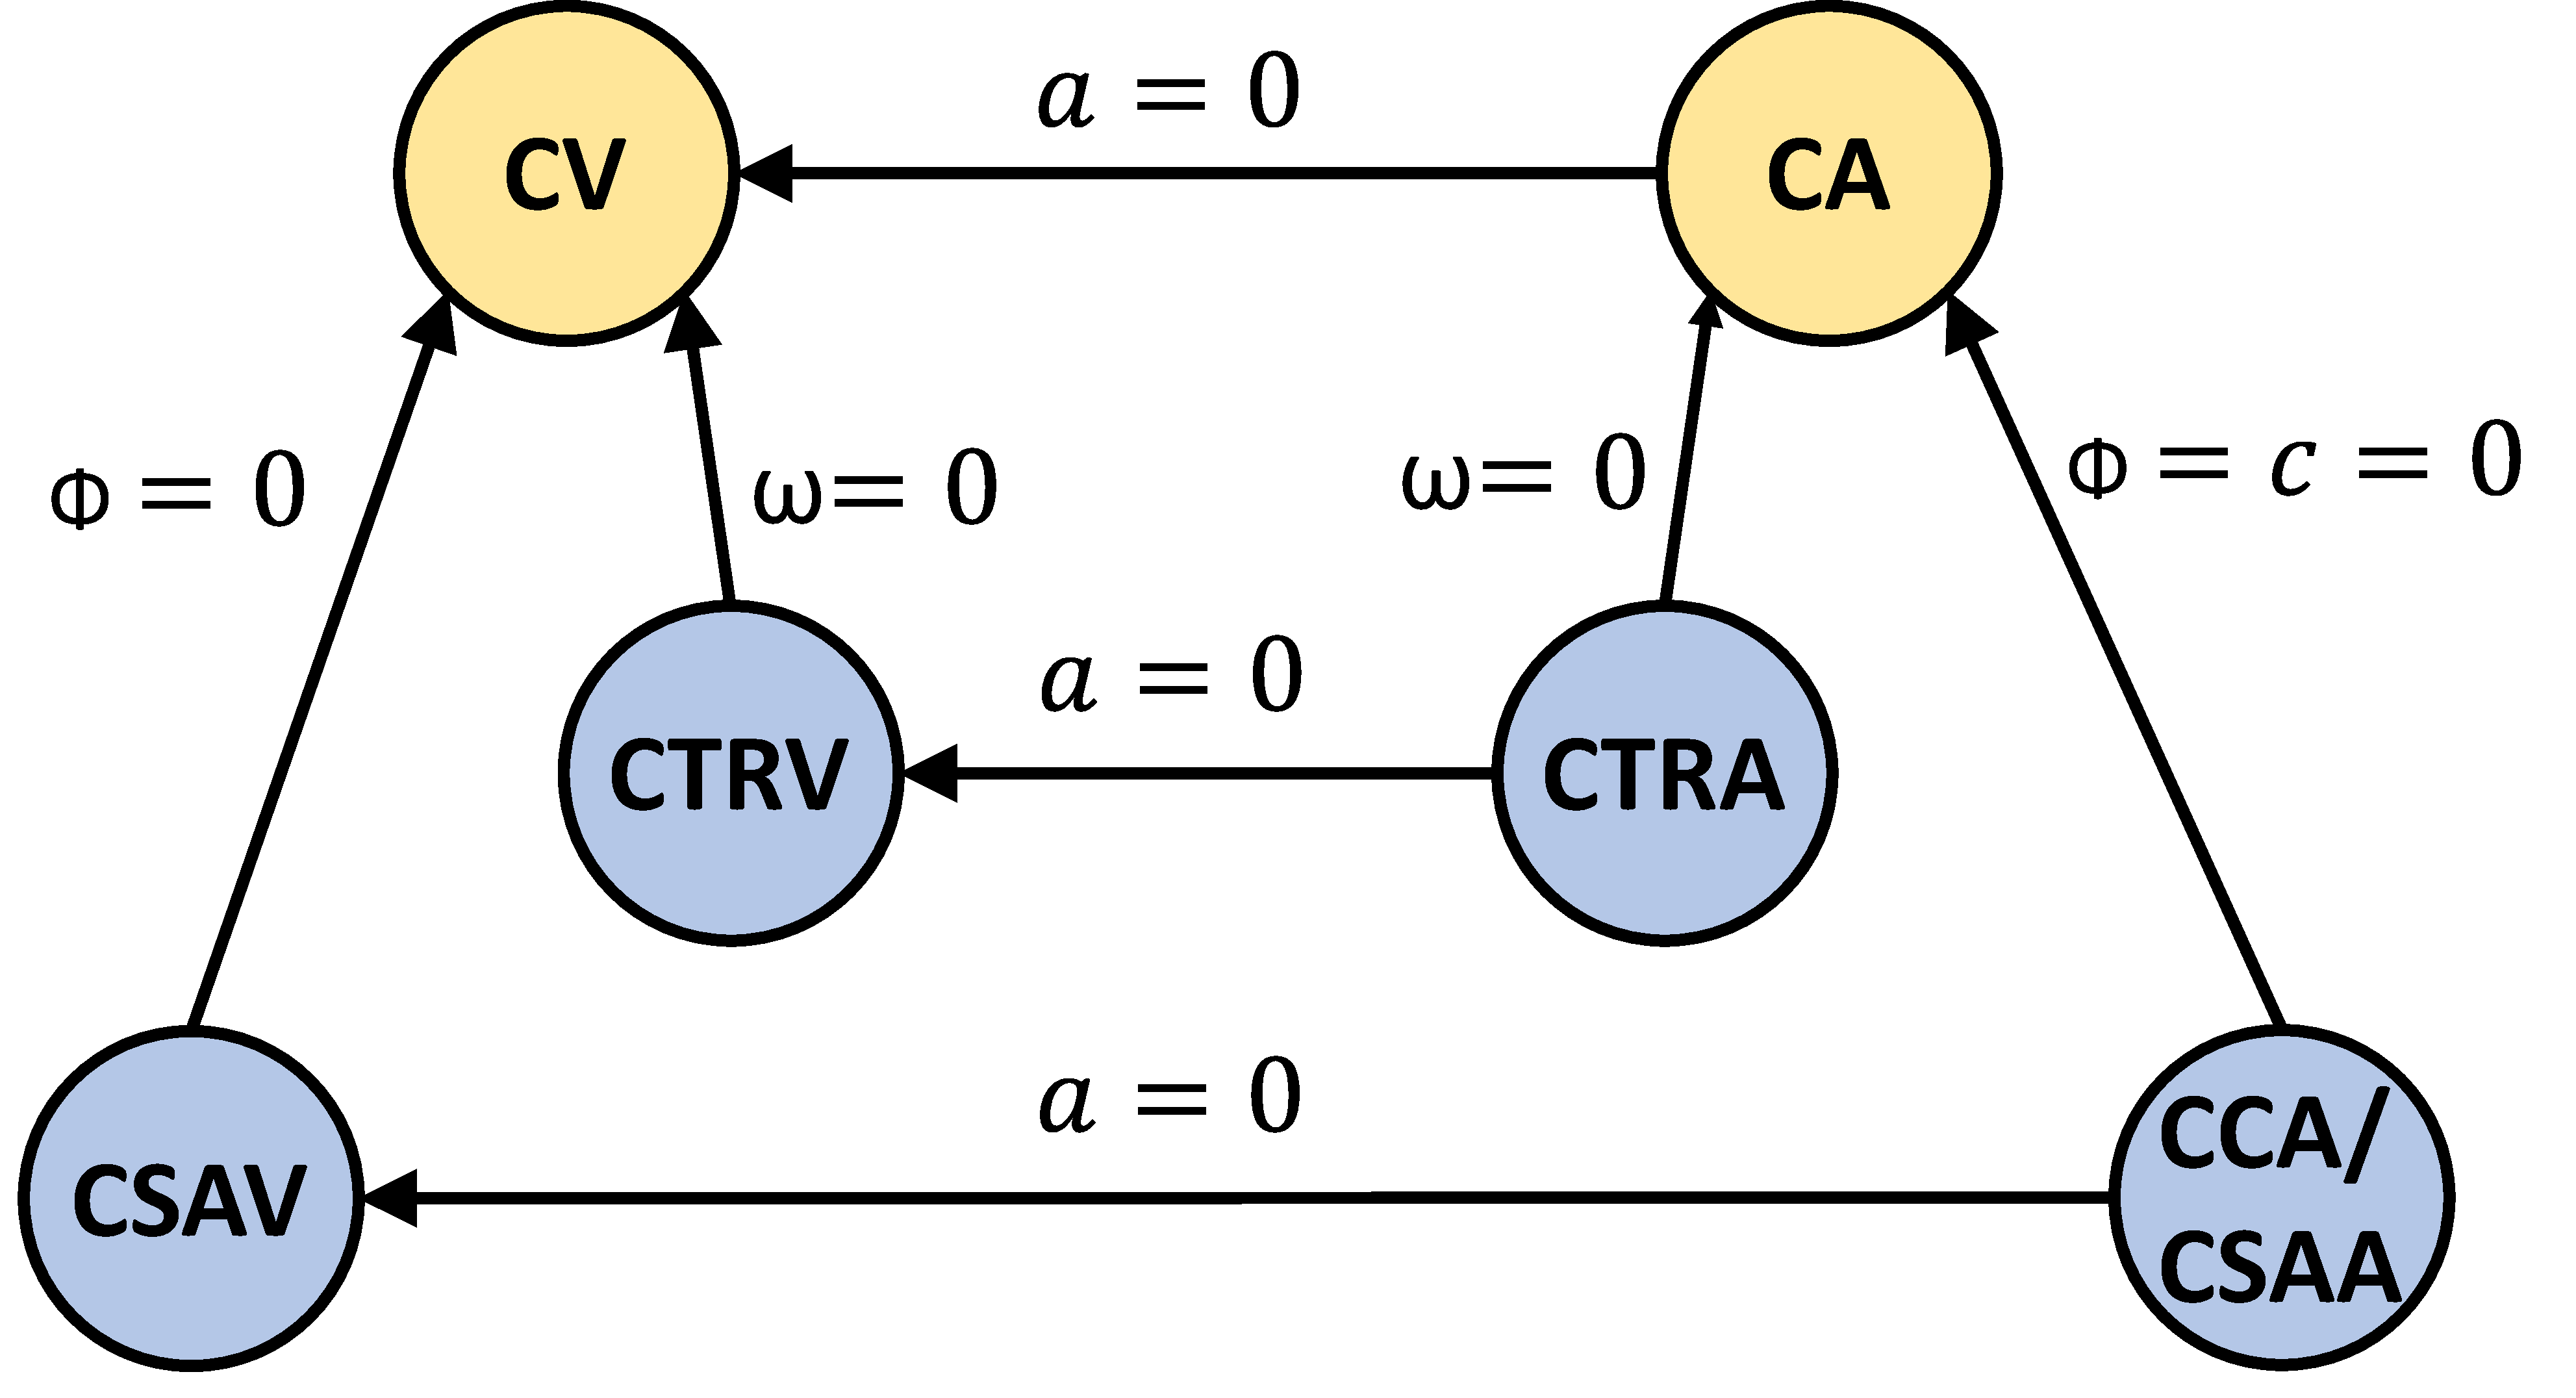
\includegraphics[width=0.6\linewidth]{chapter_3_theoretical_background/linear_curvilinear_mp.pdf}
	\caption[Overview of Single Trajectory prediction methods]{Overview of Single Trajectory prediction methods. Every sophisticated model can be transformed into a simpler one by setting one state veriable to zero}
	Source: \textit{Comparison and evaluation of advanced motion models for vehicle tracking} \cite{schubert2008comparison}
	\label{fig:chapter_3_theoretical_background/linear_curvilinear_mp}
\end{figure}

Several single-trajectory prediction models have been proposed in the literature, including Constant Velocity (CV), Constant Acceleration (CA), Constant Turn Rate and Velocity (CTRV), Constant Turn Rate and Acceleration (CTRA), Constant Speed and Angular Velocity (CSAV), and Constant Curvature Acceleration (CCA)/Constant Speed and Angular Acceleration (CSAA), as illustrated in Figure \ref{fig:chapter_3_theoretical_background/linear_curvilinear_mp}:

\begin{itemize}
	\item Constant Velocity (CV) model assumes that the object moves at a constant velocity and its future position can be predicted by simply extrapolating its current velocity vector. This model is simple and computationally efficient, but it may not accurately capture the object's motion if it changes its velocity.
	\item Constant Acceleration (CA) model is an extension of the CV model, assuming that the object can also change its acceleration in a linear manner. This model can provide more accurate predictions of the object's future position and velocity, but it may not be suitable for objects with more complex motion patterns.
	\item Constant Turn Rate and Velocity (CTRV) model assumes that the object moves in a circular trajectory with a constant turn rate and velocity magnitude. This model is useful for predicting the motion of objects such as drones or missiles, but it may not accurately represent the motion of objects with more complex trajectories.
	\item Constant Turn Rate and Acceleration (CTRA) model is an extension of the CTRV model, allowing the object to change its acceleration while maintaining a constant turn rate. This model is often used in applications such as autonomous driving or aircraft navigation, where objects can accelerate or decelerate.
	\item Constant Speed and Acceleration Vector (CSAV) model assumes that the object moves along a straight line with a constant speed and acceleration vector. This model can be useful for predicting the motion of objects such as trains or boats.
	\item Constant Acceleration and Angle (CAA) model assumes that the object moves along a constant heading angle and can change its acceleration in a linear manner. This model can be useful for predicting the motion of objects such as bicycles or motorcycles.
\end{itemize}

It can be observed how a sophisticated model can be transformed into a simpler one by setting one state veriable to zero. For example, CTRA is transformed to CTRV if the agent acceleration $a$ is set to zero. Similarly, CTRA is transformed to CA if the angular speed $\omega$ is set to 0. In this Section we particularly focus on the prediction equations and differences of the most commonly used single-trajectory prediction methods in the field of \ac{AD} to predict the future motion of a moving object: CTRV and CTRA.

\subsubsection{Constant Turn Rate Velocity (CTRV)}
\label{subsubsec:3_CTRV}

The Constant Turn Rate and Velocity (CTRV) model is a mathematical model used in the field of autonomous navigation to predict the future motion of a moving object. The model assumes that the object moves along a smooth, continuous path, and that its velocity and turn rate are constant.

The model describes the motion of the object using a set of differential equations that relate the rate of change of the object's state to its current state and any external inputs. The state of the object is described using five variables: the x and y coordinates of its position, its velocity magnitude, its heading angle (or direction of travel), and its turn rate.

The CTRV model predicts the future position of the object by using the current position, velocity, heading angle, and turn rate, and propagating them forward in time. The model assumes that the velocity and turn rate remain constant throughout the prediction interval.

The prediction equations for the CTRV model are described as follows:

\begin{equation}
\begin{split}
	x_{k+1} &= x_k + \frac{v_k}{\omega_k}\left[\sin(\psi_k+\omega_k\Delta t)-\sin(\psi_k)\right] \\
	y_{k+1} &= y_k + \frac{v_k}{\omega_k}\left[\cos(\psi_k)-\cos(\psi_k+\omega_k\Delta t)\right] \\
	v_{k+1} &= v_k \\
	\psi_{k+1} &= \psi_k + \omega_k\Delta t \\
	\omega_{k+1} &= \omega_k
\end{split}
\end{equation}
	
where:

$x_k$ and $y_k$ are the coordinates of the object's position at time step $k$
$v_k$ is the velocity magnitude at time step $k$
$\psi_k$ is the heading angle (in radians) at time step $k$
$\omega_k$ is the turn rate (in radians per second) at time step $k$
$\Delta t$ is the time step size.

The first two equations predict the object's position at the next time step, based on its current position, velocity, heading angle, and turn rate. The third and fifth equations predict that the velocity and turn rate will remain constant. The fourth equation predicts the object's heading angle at the next time step, based on its current heading angle and turn rate.

Overall, the CTRV model is a useful tool for predicting the motion of a moving object and can be used in a variety of applications, such as robotics, aviation, and space exploration.

\subsubsection{Constant Turn Rate Acceleration (CTRA)}
\label{subsubsec:3_CTRA}

The Constant Turn Rate and Acceleration (CTRA) model is an extension of the Constant Turn Rate and Velocity (CTRV) model, allowing the object to change its acceleration while maintaining a constant turn rate. This makes the CTRA model more accurate for predicting the motion of objects that can accelerate or decelerate, such as cars or aircraft.

The state of the object in the CTRA model is described using variables such as the x and y coordinates of its position, its velocity magnitude, its heading angle, its turn rate, and its acceleration magnitude. The motion of the object is modeled using the following set of equations:

\begin{equation}
\begin{split}
		x_{k+1} &= x_k + \frac{v_k}{\omega_k} \left[ \sin(\theta_k + \omega_k \Delta t) - \sin(\theta_k) \right] \\
		y_{k+1} &= y_k - \frac{v_k}{\omega_k} \left[ \cos(\theta_k + \omega_k \Delta t) - \cos(\theta_k) \right] \\
		\theta_{k+1} &= \theta_k + \omega_k \Delta t \\
		v_{k+1} &= v_k + a_k \Delta t \\
		\omega_{k+1} &= \omega_k
\end{split}
\end{equation}

where $x_k$ and $y_k$ are the object's position coordinates at time $k$, $\theta_k$ is its heading angle, $v_k$ is its velocity magnitude, $\omega_k$ is its turn rate, and $a_k$ is its acceleration magnitude. $\Delta t$ is the time step between predictions.

The first two equations describe the object's position updates based on its current position, velocity, heading angle, turn rate, and the time step. The third equation describes the object's heading angle update based on its current heading angle and turn rate. The fourth equation describes the object's velocity update based on its current velocity and acceleration. The last equation assumes that the object's turn rate remains constant over time.

In summary, the CTRA model is a useful tool for predicting the motion of objects that can accelerate or decelerate while maintaining a constant turn rate. The model's equations include variables such as the object's position, velocity, heading angle, turn rate, and acceleration magnitude, and they are based on the kinematic equations of motion.

\subsubsection{CTRV vs CTRA}
\label{subsubsec:3_CTRV_vs_CTRA}

The CTRV model assumes that the object moves along a smooth, continuous path, and that its velocity and turn rate are constant. This means that the object moves in a circular trajectory with a fixed radius. The state of the object is described using variables such as the x and y coordinates of its position, its velocity magnitude, its heading angle, and its turn rate.

On the other hand, the CTRA model assumes that the object can change its acceleration while maintaining a constant turn rate. This makes the CTRA model more accurate for predicting the motion of objects that can accelerate or decelerate, such as cars or aircraft. The state of the object in the CTRA model is described using similar variables to the CTRV model, but with an additional variable to represent the object's acceleration.

The prediction equations for the CTRV model are based on the kinematic equations for circular motion, where the object's position, velocity, and heading angle change in a continuous and smooth manner. In contrast, the prediction equations for the CTRA model include an additional term for the object's acceleration, which allows for more accurate predictions of the object's future motion when it can accelerate or decelerate.

In terms of implementation, the CTRA model requires more computational resources due to the additional term for acceleration, which increases the complexity of the equations. This can make the CTRV model more computationally efficient and faster to calculate in real-time applications. However, the CTRA model is more accurate in predicting the motion of objects with varying acceleration and is often used in applications such as autonomous driving or aircraft navigation.

In summary, the main differences between the CTRV and CTRA prediction models are that the CTRA model includes an additional term for acceleration in its prediction equations, allowing for more accurate predictions of the motion of objects with varying acceleration, while the CTRV model assumes a constant velocity and turn rate and is more computationally efficient.

\section{Deep Learning algorithms}
\label{sec:3_dlb_formulation}

In this section the mathematical formulation of the \ac{DL} layers employed in this thesis is covered. In particular, these are the 1D-\ac{CNN}, \ac{LSTM}, \ac{GAN}, Attention mechanism and \ac{GNN} layers. We briefly introduce each layer, as well as the corresponding mathematical formulation to enhance the comprehension of the learning-based methods proposed in this thesis.

\subsection{Convolutional Neural Networks}
\label{subsec:3_cnns}

% Additional info

% https://towardsdatascience.com/understanding-1d-and-3d-convolution-neural-network-keras-9d8f76e29610
% file:///C:/Users/Carlos/Downloads/sensors-22-09517.pdf
% https://e2eml.school/convolution_one_d.html
% https://arxiv.org/pdf/1512.07108.pdf

Convolutional neural networks (CNNs) are commonly used for image and signal processing tasks. The type of CNN architecture used depends on the nature of the input data. Here are the differences between the three types of CNNs:

\begin{itemize}
	\item 1D Convolutional Neural Networks (1D CNNs): 1D CNNs are used for processing sequential data such as time series data, speech signals, and text data. The input to a 1D CNN is a one-dimensional sequence of data, such as a time series of sensor readings. 1D CNNs typically have fewer parameters and are computationally efficient compared to 2D and 3D CNNs.
	
	\item 2D Convolutional Neural Networks (2D CNNs): 2D CNNs are used for processing 2D images. The input to a 2D CNN is a two-dimensional image represented as a matrix of pixels. The convolutional layers in a 2D CNN apply filters that slide over the image to extract local features. The output of each convolutional layer is a set of 2D feature maps. 2D CNNs are widely used for image classification, object detection, and image segmentation.
	
	\item 3D Convolutional Neural Networks (3D CNNs): 3D CNNs are used for processing 3D volumetric data such as CT scans, MRI images, and video data. The input to a 3D CNN is a three-dimensional volume represented as a sequence of 2D images. The convolutional layers in a 3D CNN apply filters that slide over the 3D volume to extract local features. The output of each convolutional layer is a set of 3D feature maps. 3D CNNs are used for tasks such as medical image analysis, video classification, and action recognition.
\end{itemize}

In summary, 1D CNNs are used for processing sequential data (such as time series data, audio signals, and text), 2D CNNs are used for image processing, and 3D CNNs are used for volumetric data. As we will see in Chapter \ref{cha:predictive_techniques_in_ad}, in this work we focus on 1D CNNs. The basic building blocks of a 1D CNN are convolutional layers, which learn local patterns in the input data by applying a set of filters to it, as illustrated in Figure \ref{fig:chapter_3_theoretical_background/CNN_1D}. Each filter slides over the input sequence and performs a dot product operation at each position to generate a feature map. These feature maps capture the presence of certain patterns at different positions in the input sequence. 
 
The architecture of a 1D CNN typically consists of several convolutional layers, followed by one or more fully connected layers for classification or regression. The output of each convolutional layer is fed into the next layer, with optional pooling layers in between to reduce the spatial dimension of the feature maps. The final output of the network is obtained by passing the output of the last fully connected layer through a suitable activation function, such as softmax for classification or linear for regression.
 
 \begin{figure}[h]
 	\centering
 	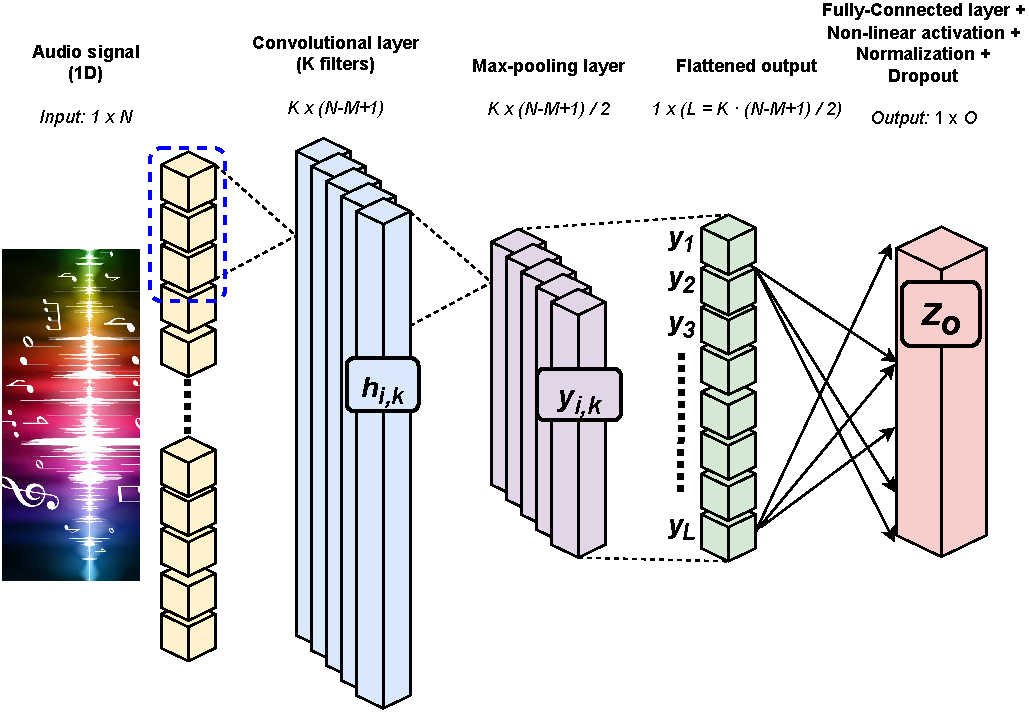
\includegraphics[width=0.6\linewidth]{chapter_3_theoretical_background/CNN_1D.pdf}
 	\caption{Example of CNN architecture to process 1D-input signals}
 	\label{fig:chapter_3_theoretical_background/CNN_1D}
 \end{figure}
 
Let $x$ be a 1-dimensional input sequence of length $n$, represented as a vector $x = [x_1, x_2, ..., x_n]$. Let $k$ be a filter of length $m$, represented as a vector $k = [k_1, k_2, ..., k_m]$. We can apply the filter $k$ to the input sequence $x$ by computing a convolution operation:

\begin{equation}
	(k * x)_i = \sum_{j=1}^m k_j x_{i+j-m}
\end{equation}

where $*$ denotes the convolution operation, and $i$ ranges from $m$ to $n$. This operation produces a new sequence of length $n - m + 1$, representing the local features extracted from the input sequence $x$ by the filter $k$.

To learn multiple filters and extract different types of features, we use multiple convolutional layers in the network. Each layer applies a set of filters, and produces a set of feature maps. The feature maps can be computed as:

\begin{equation}
h_{i,j} = f(\sum_{k=1}^m W_{j,k} x_{i+k-m} + b_j)
\end{equation}

where $h$ is the feature map at position $i$ and filter $j$, $W$ is the weight matrix of the $j$-th filter, $b$ is the bias term for the $j$-th filter, and $f$ is an activation function (such as ReLU or sigmoid).

After each convolutional layer, we typically apply a pooling layer to reduce the dimensionality of the features and increase the translation invariance of the network. The most common pooling operation is max pooling, which selects the maximum value within a window of size $p$:

\begin{equation}
y_{i,j} = \max_{k=0}^{p-1} h_{i+k,j}
\end{equation}

where $y$ is the output of the pooling layer at position $i$ and filter $j$.

Finally, we can use one or more fully connected layers to perform the final classification or regression task. The output of the pooling layer is flattened into a vector, and fed into a set of fully connected layers, with optional dropout regularization and batch normalization:

\begin{equation}
z_j = f(\sum_{i=1}^n W_{i,j} y_i + b_j)
\end{equation}

where $z$ is the output of the $j$-th fully connected layer, $W$ is the weight matrix, $y$ is the flattened output of the pooling layer, $b$ is the bias term, and $f$ is an activation function. 

\subsection{Recurrent Neural Networks}
\label{subsec:3_rnns}

Recurrent Neural Networks (RNNs) are a type of neural network that are designed to process sequential data, where the order of the input matters. They are widely used in a variety of applications such as natural language processing, speech recognition, image captioning, and time series prediction.

The general theory of RNNs is that they have a feedback loop in their architecture that allows information to be passed from one time step to the next, thereby enabling the network to capture dependencies between the inputs at different time steps. The input at each time step is fed into the network along with the output from the previous time step, and the network uses this information to generate a new output.

There are several types of RNNs, including the basic RNN, the Gated Recurrent Unit (GRU), and the Long Short-Term Memory (LSTM) \cite{hochreiter1997long}. The basic RNN is the simplest form of RNN, where the output at each time step is a function of the input at that time step and the output from the previous time step. However, it suffers from the vanishing gradient problem, where the gradients become exponentially small as they propagate through time, making it difficult to learn long-term dependencies.

The GRU is a variation of the basic RNN that uses gating mechanisms to control the flow of information through the network. It has fewer parameters than the LSTM and can be faster to train, but it may not perform as well as the LSTM on tasks that require more complex temporal dependencies.

\subsubsection{Long Short-Term Memory}
\label{subsubsec:3_LSTMs}

LSTM networks were introduced to address the vanishing gradient problem in standard RNNs. They achieve this by using a memory cell to store information over long periods of time, and three gating mechanisms to control the flow of information through the network. Figure \ref{fig:chapter_3_theoretical_background/LSTM} provides a detailed overview of the LSTM cell structure, illustrating the workflow from the previous cell output and input at time $t-1$ in order to compute the current cell state and hidden state at time $t$.

\begin{figure}[h]
	\centering
	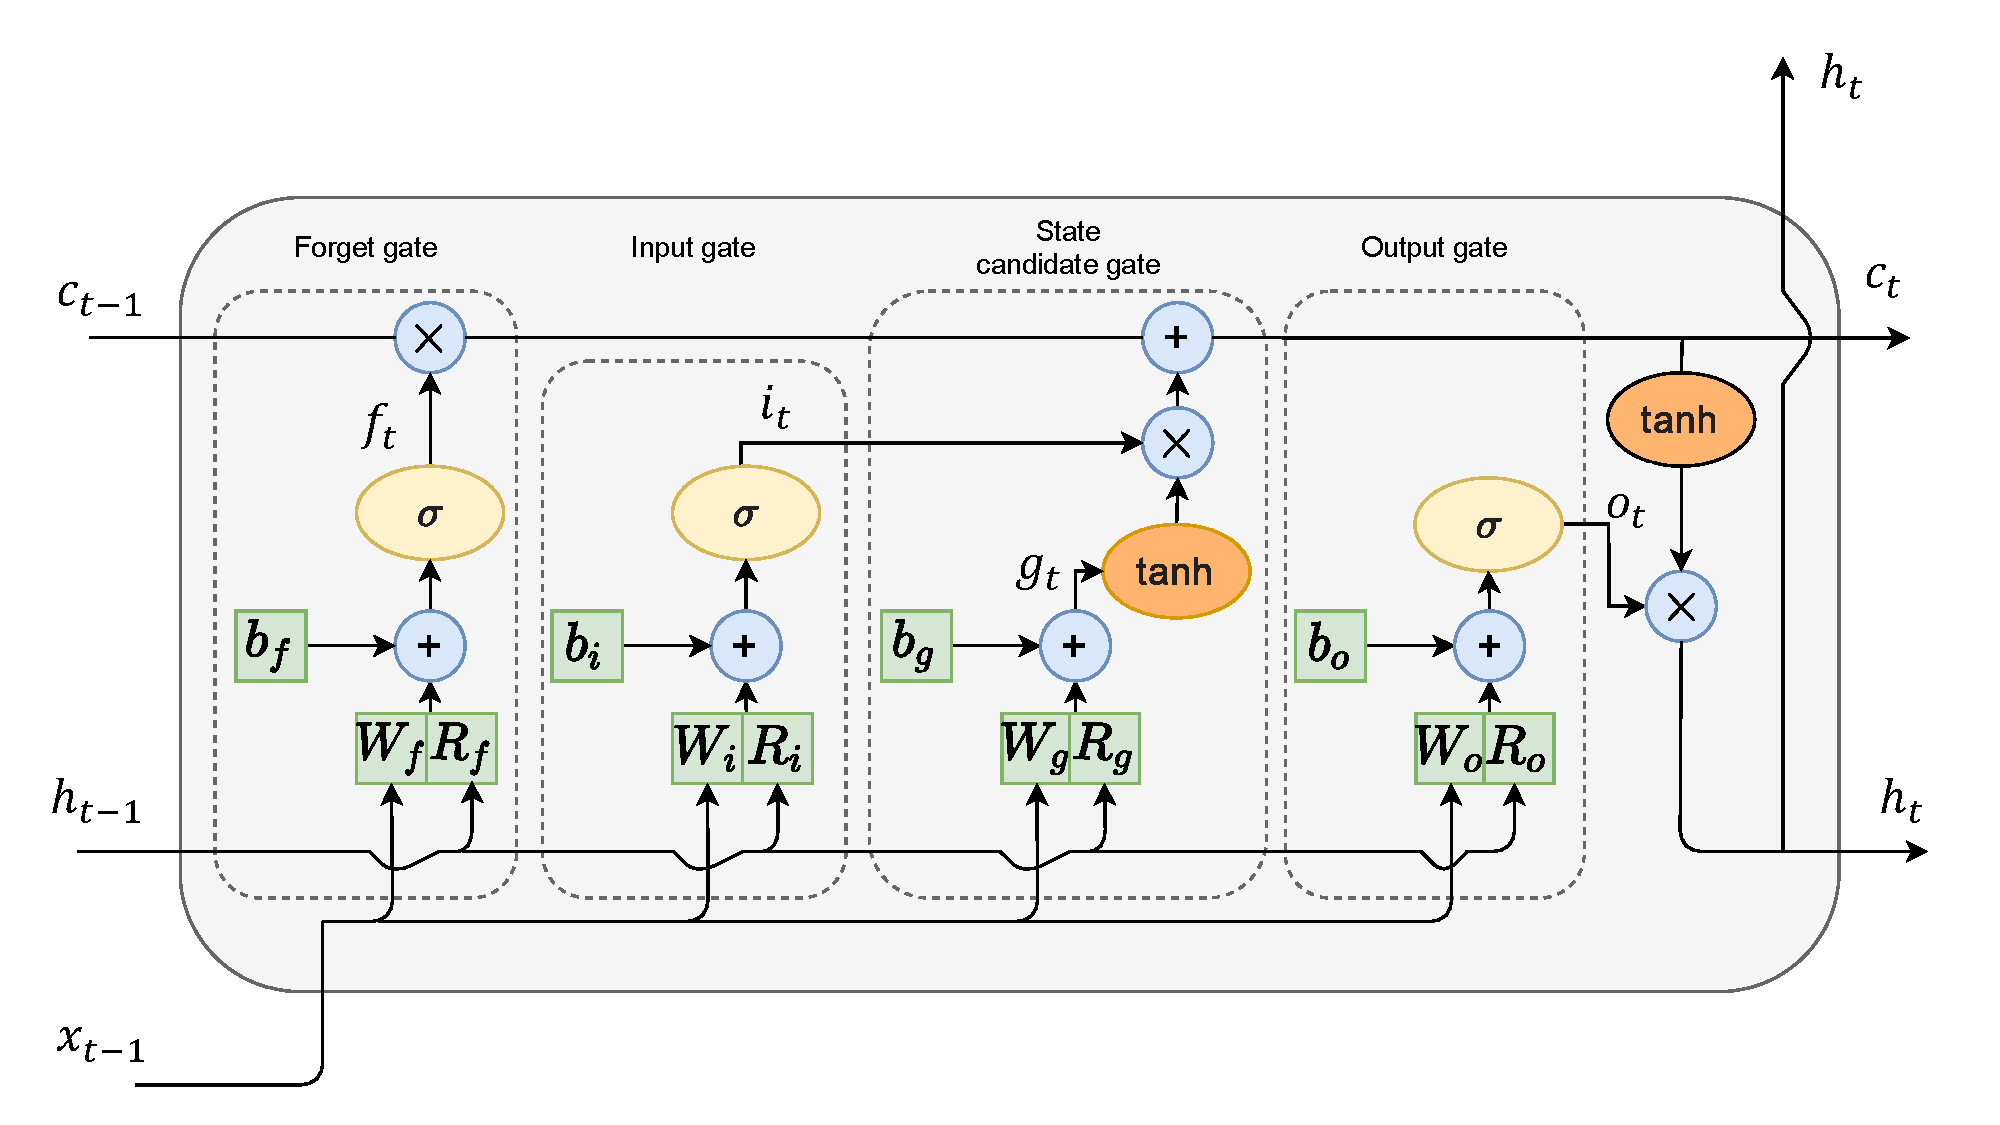
\includegraphics[width=\linewidth]{chapter_3_theoretical_background/LSTM_cell.pdf}
	\caption{Overview of the LSTM cell structure}
	\label{fig:chapter_3_theoretical_background/LSTM}
\end{figure}

The three gates are called the input gate, forget gate, and output gate, and they are responsible for deciding which information to store in the memory cell, which information to forget, and which information to output, respectively.

The equations for the input, forget, and output gates are as follows:

\begin{itemize}
	\item Input gate: $i_t = \sigma(W_i \cdot [h_{t-1}, x_t] + b_i)$
	\item Forget gate: $f_t = sigmoid(W_f * [h_{t-1}, x_t] + b_f)$
	\item Input gate: $o_t = sigmoid(W_o * [h_{t-1}, x_t] + b_o)$
\end{itemize}

where $x_t$ is the input at time $t$, $h_{t-1}$ is the hidden state from the previous time step, $i_t$ is the input gate activation, $f_t$ is the forget gate activation, and $o_t$ is the output gate activation. $W_i$, $W_f$, and $W_o$ are weight matrices, and $b_i$, $b_f$, and $b_o$ are bias vectors.

On the other hand, the memory cell is updated based on the input, forget, and output gates, as well as a new candidate value that is computed based on the current input and hidden state. The equations for the memory cell and candidate value are as follows:

\begin{equation}
\begin{split}
		\tilde{C}t &= \tanh(W_c \cdot [h{t-1}, x_t] + b_c) \\
		C_t &= f_t \cdot C_{t-1} + i_t \cdot \tilde{C}_t 
\end{split}
\end{equation}

where $\tilde{C}t$ is the candidate value, $C_t$ is the new memory cell value, and $C{t-1}$ is the previous memory cell value. $W_c$ is a weight matrix and $b_c$ is a bias vector.

Finally, the hidden state at time $t$ is computed based on the output gate and the new memory cell value, using the following equation:

\begin{equation}
	h_t = o_t \cdot \tanh(C_t)
\end{equation}

This equation scales the memory cell value by the output gate activation, then applies a hyperbolic tangent function to obtain the new hidden state.

In summary, LSTMs use a memory cell and three gating mechanisms to learn long-term dependencies in sequential data. The input, forget, and output gates control the flow of information through the network, while the memory cell stores information over time. The equations for LSTMs involve computing the input, forget, and output gate activations, the candidate value, the new memory cell value, and the new hidden state.

\subsection{Generative Adversarial Networks}
\label{subsec:3_gans}

A discriminative model is a type of machine learning model that learns the relationship between the input features and the target output directly. The goal of a discriminative model is to learn a decision boundary that separates different classes in the input data. In other words, discriminative models focus on learning the conditional probability distribution of the target variable given the input features.

Discriminative models are often used in supervised learning tasks, such as classification and regression, where the goal is to predict a target variable based on a set of input features. Common examples of discriminative models include logistic regression, support vector machines, and neural networks.

Unlike generative models, which learn the joint probability distribution of the input and target variables, discriminative models do not model the probability distribution of the input data explicitly. Instead, they focus on learning a mapping function that directly maps the input features to the target output.

In 2014, a breakthrough paper introduced Generative adversarial networks (GANs) \cite{goodfellow2020generative}, a clever new way to leverage the power of discriminative models to get good generative models. At their heart, GANs rely on the idea that a data generator is good if we cannot tell fake data apart from real data. In statistics, this is called a two-sample test - a test to answer the question whether datasets $X=\{x_1,\ldots, x_n\}$ and $X'=\{x'_1,\ldots, x'_n\}$ were drawn from the same distribution. This allows to improve the data generator until it generates something that resembles the real data. At the very least, it needs to fool the classifier even if our classifier is a state of the art deep neural network. GANs are a powerful technique for generating realistic samples that are similar to some training data. A GAN consists of two neural networks, a generator network and a discriminator network. The generator and discriminator networks are trained in a two-player game, where the generator tries to produce samples that fool the discriminator, and the discriminator tries to correctly classify between real and generated data. The objective function for a GAN is a min-max game between the generator and discriminator, and can be optimized using gradient descent or some other optimization algorithm. Some common applications where GANs are widely used are generating realistic images, videos, audio, data augmentation or style transfer.

The generator network takes as input a random noise vector, and generates a sample that is meant to mimic real data. The discriminator network takes as input a sample, and tries to distinguish between real data and generated data. The two networks are trained in a two-player game, where the generator tries to produce samples that fool the discriminator, and the discriminator tries to correctly classify between real and generated data.

The objective function for a GAN can be formulated as a min-max game between the generator and discriminator. The generator tries to minimize the probability that the discriminator correctly classifies the generated samples as fake, while the discriminator tries to maximize the probability that it correctly classifies the real and generated samples.

The objective function for a GAN can be written as:

\begin{equation}
\begin{split}
	\min_{\theta_G}\max_{\theta_D} V(D, G) = \mathbb{E}{x\sim p{data}(x)}[\log D(x)] + \mathbb{E}{z\sim p_z(z)}[\log(1-D(G(z)))] \\
	= \mathbb{E}{x\sim p_{data}(x)}[\log D(x)] + \mathbb{E}_{z\sim p_z(z)}[\log(1-D(G(z;\theta_G)))]
\end{split}
\end{equation}

where $\theta_G$ and $\theta_D$ are the parameters of the generator and discriminator networks, respectively, $x$ is a real sample from the training data distribution $p_{data}$, $z$ is a noise vector sampled from a prior distribution $p_z$, and $G(z;\theta_G)$ is the generated sample from the generator network.

The first term of the objective function represents the expected log-probability of the discriminator correctly classifying a real sample as real. The second term represents the expected log-probability of the discriminator correctly classifying a generated sample as fake.

During training, the generator network is updated to minimize the objective function with respect to $\theta_G$, while the discriminator network is updated to maximize the objective function with respect to $\theta_D$. This can be done using gradient descent or some other optimization algorithm.

There are some well-known types of GANs, such as:

\begin{itemize}
	\item Deep Convolutional GANs (DCGANs): These are GANs that use convolutional neural networks (CNNs) in the generator and discriminator networks. DCGANs are commonly used for image generation and have been shown to produce high-quality, realistic images.
	\item Wasserstein GANs (WGANs): These are GANs that use the Wasserstein distance instead of the traditional Kullback-Leibler (KL) divergence or Jensen-Shannon (JS) divergence for measuring the difference between the real and generated distributions. WGANs have been shown to produce more stable training and generate higher-quality samples.
	\item CycleGANs: These are GANs that are designed for image-to-image translation tasks, where the goal is to transform an image from one domain to another. CycleGANs use two generators and two discriminators to learn the mapping between the two domains.
\end{itemize}

Nevertheless, in this work we focus on a particular type of GAN, known as conditional GAN or cGAN, where the generator is conditioned on some additional information, such as class labels or image annotations. The additional information is used to control the generated output, allowing for more specific generation of data. 

\subsubsection{GAN vs cGAN}
\label{subsubsec:3_cGAN}

The main difference between the original GAN and cGAN is that the original GAN generates samples without any control over the generated output, whereas the cGAN generates samples conditioned on some additional information.

In the original GAN, the generator network takes as input a random noise vector, and generates a sample that is meant to mimic real data. The discriminator network takes as input a sample, and tries to distinguish between real data and generated data. The goal of the original GAN is to train the generator network to generate samples that are indistinguishable from real data.

\begin{figure}[h]
	\centering
	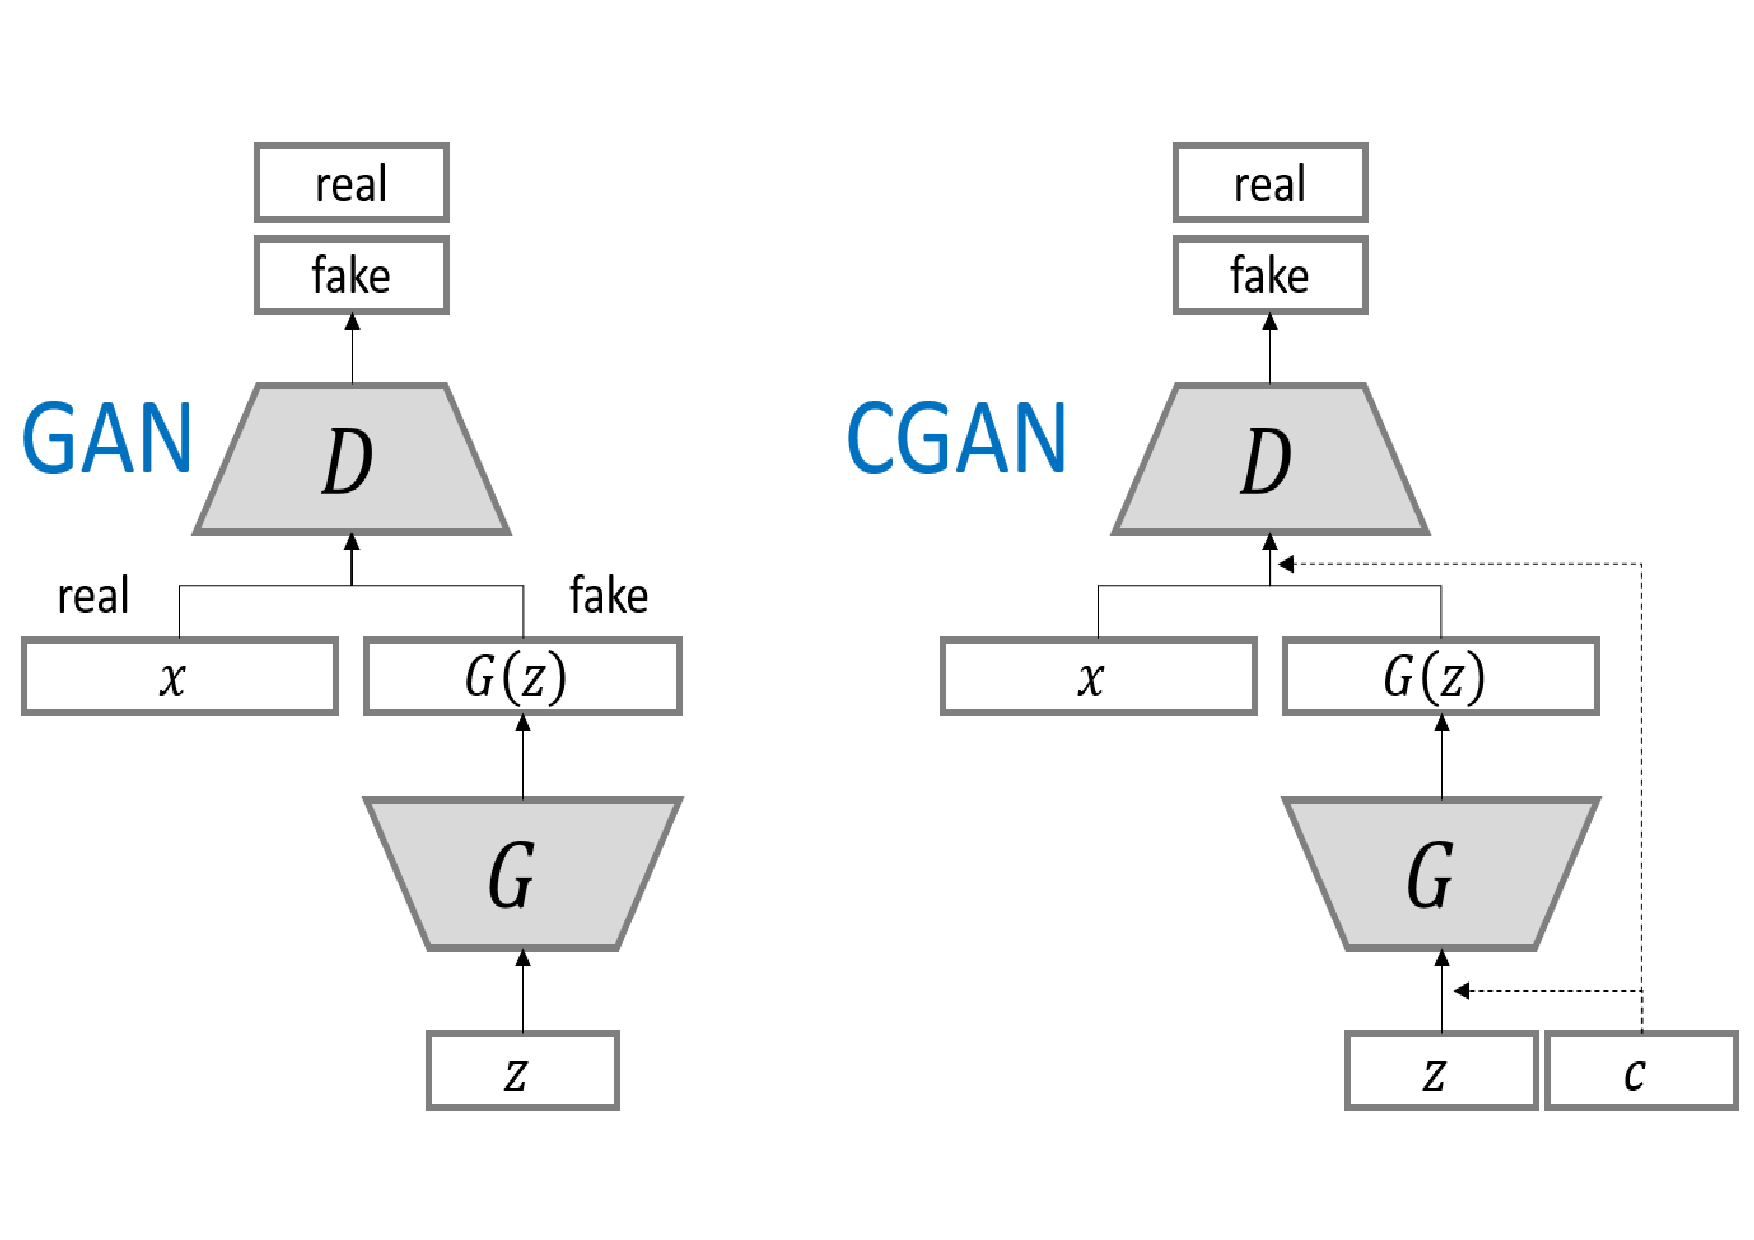
\includegraphics[width=0.5\linewidth]{chapter_3_theoretical_background/GAN.pdf}
	\caption{Comparison between the original Generative Adversarial Network (GAN) and conditional GAN (cGAN)}
	\label{fig:chapter_3_theoretical_background/GAN}
\end{figure}

In contrast, a cGAN is a GAN that is conditioned on some additional information, such as class labels or image annotations. The generator network in a cGAN takes as input both a random noise vector and a condition vector, and generates a sample that is conditioned on the additional information. The discriminator network also takes as input both the sample and the condition vector, and tries to distinguish between real data and generated data based on the condition. Figure \ref{fig:chapter_3_theoretical_background/GAN} illustrates the differences between the original GAN and the corresponding conditioned architecture.

The cGAN can be used for a variety of applications, such as image-to-image translation, where the additional information is an input image that is translated to a different output image. For example, a cGAN can be trained to convert grayscale images to color images, or to transform images of one type of object to another type of object.

The training process for a cGAN is similar to that of the original GAN, but the loss function for the generator and discriminator networks are modified to include the condition vector. Specifically, the loss function for the generator network includes a term that measures how well the generated samples match the condition vector, in addition to the term that measures how well the generated samples fool the discriminator. Similarly, the loss function for the discriminator network includes a term that measures how well the discriminator can identify the condition vector, in addition to the term that measures how well it can distinguish between real and generated data.

The cGAN can be used for a variety of applications, such as image-to-image translation, where the additional information is an input image that is translated to a different output image. For example, a cGAN can be trained to convert grayscale images to color images, or to transform images of one type of object to another type of object.

\subsection{Attention Mechanism}
\label{subsec:3_attention}

The attention mechanism is a computational method used in deep learning models to help the model focus on the most important parts of the input data. It is commonly used in natural language processing, speech recognition, and computer vision.

The basic idea of attention is to compute a set of weights that indicate the relative importance of different parts of the input. These weights are then used to compute a weighted sum of the input, which is used as the output of the attention mechanism.

The attention mechanism can be formulated mathematically using the following equations:

First, we compute a set of "keys", "values", and a "query" vector, which are used to compute the attention weights:

\begin{equation}
\begin{split}
	K = {k_1, k_2, ..., k_n}
	V = {v_1, v_2, ..., v_n}
	q = [q_1, q_2, ..., q_d]
\end{split}
\end{equation}

where $n$ is the number of elements in the input, and $d$ is the dimension of the query vector. Next, we compute the attention weights using a function that compares the query vector to each of the keys:

\begin{equation}
	a_i = \text{softmax}(q^T k_i)
\end{equation}

where $a_i$ is the attention weight for the $i$th element of the input. Finally, we compute the output of the attention mechanism as a weighted sum of the values:

\begin{equation}
	o = \sum_{i=1}^{n} a_i v_i
\end{equation}

\subsubsection{Positional Encoding}
\label{subsubsec:3_positional_encoding}

In the attention mechanism, positional encoding is used to incorporate the order of the input sequence into the model. Positional encoding involves adding a fixed-length vector to the input embeddings that encodes the position of each element in the sequence.

The mathematical formulation of positional encoding is as follows:

\begin{equation}
	\text{PE}_{(pos,2i)} = \sin\left(\frac{pos}{10000^{2i/d}}\right)
\end{equation}

\begin{equation}
	\text{PE}_{(pos,2i+1)} = \cos\left(\frac{pos}{10000^{2i/d}}\right)
\end{equation}

where $pos$ is the position of the element in the sequence, $i$ is the index of the dimension, and $d$ is the dimension of the input embeddings. The positional encoding vectors are added to the input embeddings before they are passed through the self-attention mechanism.

The choice of the constants used in the positional encoding formulation, such as the use of the sine and cosine functions and the value of $10000$, is arbitrary but has been shown to work well in practice. The positional encoding vectors add a sinusoidal pattern to the input embeddings that allows the model to distinguish between elements at different positions in the sequence.

Positional encoding has been shown to be an effective way of incorporating sequential information into transformer-based models, and it has been used successfully in a variety of natural language processing tasks, including machine translation, language modeling, and sentiment analysis.

\subsubsection{Multi-Head Attention}
\label{subsubsec:3_multi_head_attention}

Multi-head attention is a type of attention mechanism used in deep learning models, particularly in transformer-based architectures, to allow the model to attend to multiple parts of the input simultaneously. It involves splitting the input into multiple heads and computing separate attention scores for each head, which are then combined to produce the final output.

The multi-head attention mechanism can be formulated mathematically using the following equations:

First, we split the keys, values, and query vectors into multiple "heads", each of which has its own set of learned weight matrices:

\begin{equation}
	K_i = {k_{i,1}, k_{i,2}, ..., k_{i,n}}
\end{equation}

\begin{equation}
	V_i = {v_{i,1}, v_{i,2}, ..., v_{i,n}}
\end{equation}

\begin{equation}
	Q_i = {q_{i,1}, q_{i,2}, ..., q_{i,n}}
\end{equation}

where $n$ is the number of elements in the input, and $i$ is the index of the head.

Next, we compute the attention weights and outputs for each head separately, using the same equations as in the basic attention mechanism:

\begin{equation}
	a_{i,j} = \text{softmax}(Q_i^T K_{i,j})
\end{equation}

\begin{equation}
	o_{i} = \sum_{j=1}^{n} a_{i,j} V_{i,j}
\end{equation}

Finally, we concatenate the outputs from all the heads and multiply by a learned weight matrix to produce the final output:

\begin{equation}
	\text{MultiHead}(Q, K, V) = \text{Concat}(\text{head}_1, \dots, \text{head}_h)W^O
\end{equation}

where $\text{head}_i$ is the output of the $i$th head, and $h$ is the number of attention heads.

The multi-head attention mechanism allows the model to attend to multiple parts of the input at once, which can be useful for capturing complex relationships between different parts of the input. It is often used in transformer-based architectures for natural language processing and other tasks.

\subsubsection{Self-Attention vs Cross-Attention}
\label{subsubsec:3_self_attention_vs_cross_attention}

Self-attention is a type of attention mechanism used in deep learning models, particularly in transformer-based architectures, that allows the model to attend to different parts of the input sequence to compute a representation of each input element.

In self-attention, the input sequence is transformed into three different vectors: the query vector, the key vector, and the value vector. These vectors are then used to compute the attention score for each element of the input sequence with respect to every other element in the sequence. The attention scores are used to weight the value vectors, which are then combined to produce the final output.

The mathematical formulation of self-attention is as follows:

\begin{equation}
	\text{SelfAttention}(X) = \text{softmax}\left(\frac{QK^T}{\sqrt{d_k}}\right)V
\end{equation}

where $X$ is the input sequence, $Q$, $K$, and $V$ are the query, key, and value vectors, respectively, and $d_k$ is the dimension of the key vectors. The softmax function is applied row-wise to the matrix $\frac{QK^T}{\sqrt{d_k}}$, resulting in an attention matrix that has the same dimensions as $X$. The attention matrix is then used to weight the value vectors $V$, which are combined to produce the final output.

The query, key, and value vectors are obtained through linear transformations of the input embeddings. The exact way in which these transformations are carried out can vary depending on the specific architecture, but in general they involve matrix multiplications with learnable weight matrices.

Self-attention has been shown to be a powerful mechanism for capturing long-range dependencies in sequential data, and it has been used successfully in a variety of natural language processing tasks, including machine translation, language modeling, and sentiment analysis.

On the other hand, in cross-attention, one of the input sequences serves as the query sequence, while the other sequence serves as the key-value sequence. The query sequence is transformed into a query vector, while the key-value sequence is transformed into key and value vectors. The query vector is then used to compute the attention score for each element in the query sequence with respect to every element in the key-value sequence. The attention scores are used to weight the value vectors, which are then combined to produce the final output.

The mathematical formulation of cross-attention is as follows:

\begin{equation}
	\text{CrossAttention}(Q, K, V) = \text{softmax}\left(\frac{QK^T}{\sqrt{d_k}}\right)V
\end{equation}

where $Q$, $K$, and $V$ are the query, key, and value vectors, respectively, and $d_k$ is the dimension of the key vectors. The softmax function is applied row-wise to the matrix $\frac{QK^T}{\sqrt{d_k}}$, resulting in an attention matrix that has the same dimensions as the query sequence. The attention matrix is then used to weight the value vectors, which are combined to produce the final output.

Compared to self-attention, which operates on a single sequence, cross-attention operates on two sequences. The key-value sequence provides additional information that can help the model compute more accurate representations of the elements in the query sequence. Cross-attention is commonly used in machine translation models, where one of the input sequences is the source language and the other sequence is the target language.

The main differences between self-attention and cross-attention are:

Self-attention operates on a single sequence, while cross-attention operates on two sequences.
In self-attention, the query, key, and value vectors are all derived from the same input sequence, while in cross-attention, the key-value sequence provides the key and value vectors.
Self-attention is used to capture relationships between elements within a sequence, while cross-attention is used to capture relationships between elements in different sequences.

\subsubsection{Transformer}
\label{subsubsec:3_transformer}

% https://lena-voita.github.io/nlp_course/seq2seq_and_attention.html

Along this section the attention mechanism has been stated, from the main idea to the differences between self-attention and cross-attention. The Transformer model wraps-up all these concepts into a single and elegant architecture which allows the model to weigh the importance of different parts of the input sequence when computing a representation of each element in the sequence. Introduced in 2017 \cite{vaswani2017attention}, it has become the absolute standard for Natural language Processing (NLP) tasks such as language modeling, question answering or machine translation. Figure \ref{fig:chapter_3_theoretical_background/transformer} depicts the Transformer architecture proposed in the original paper.

\begin{figure}[h]
	\centering
	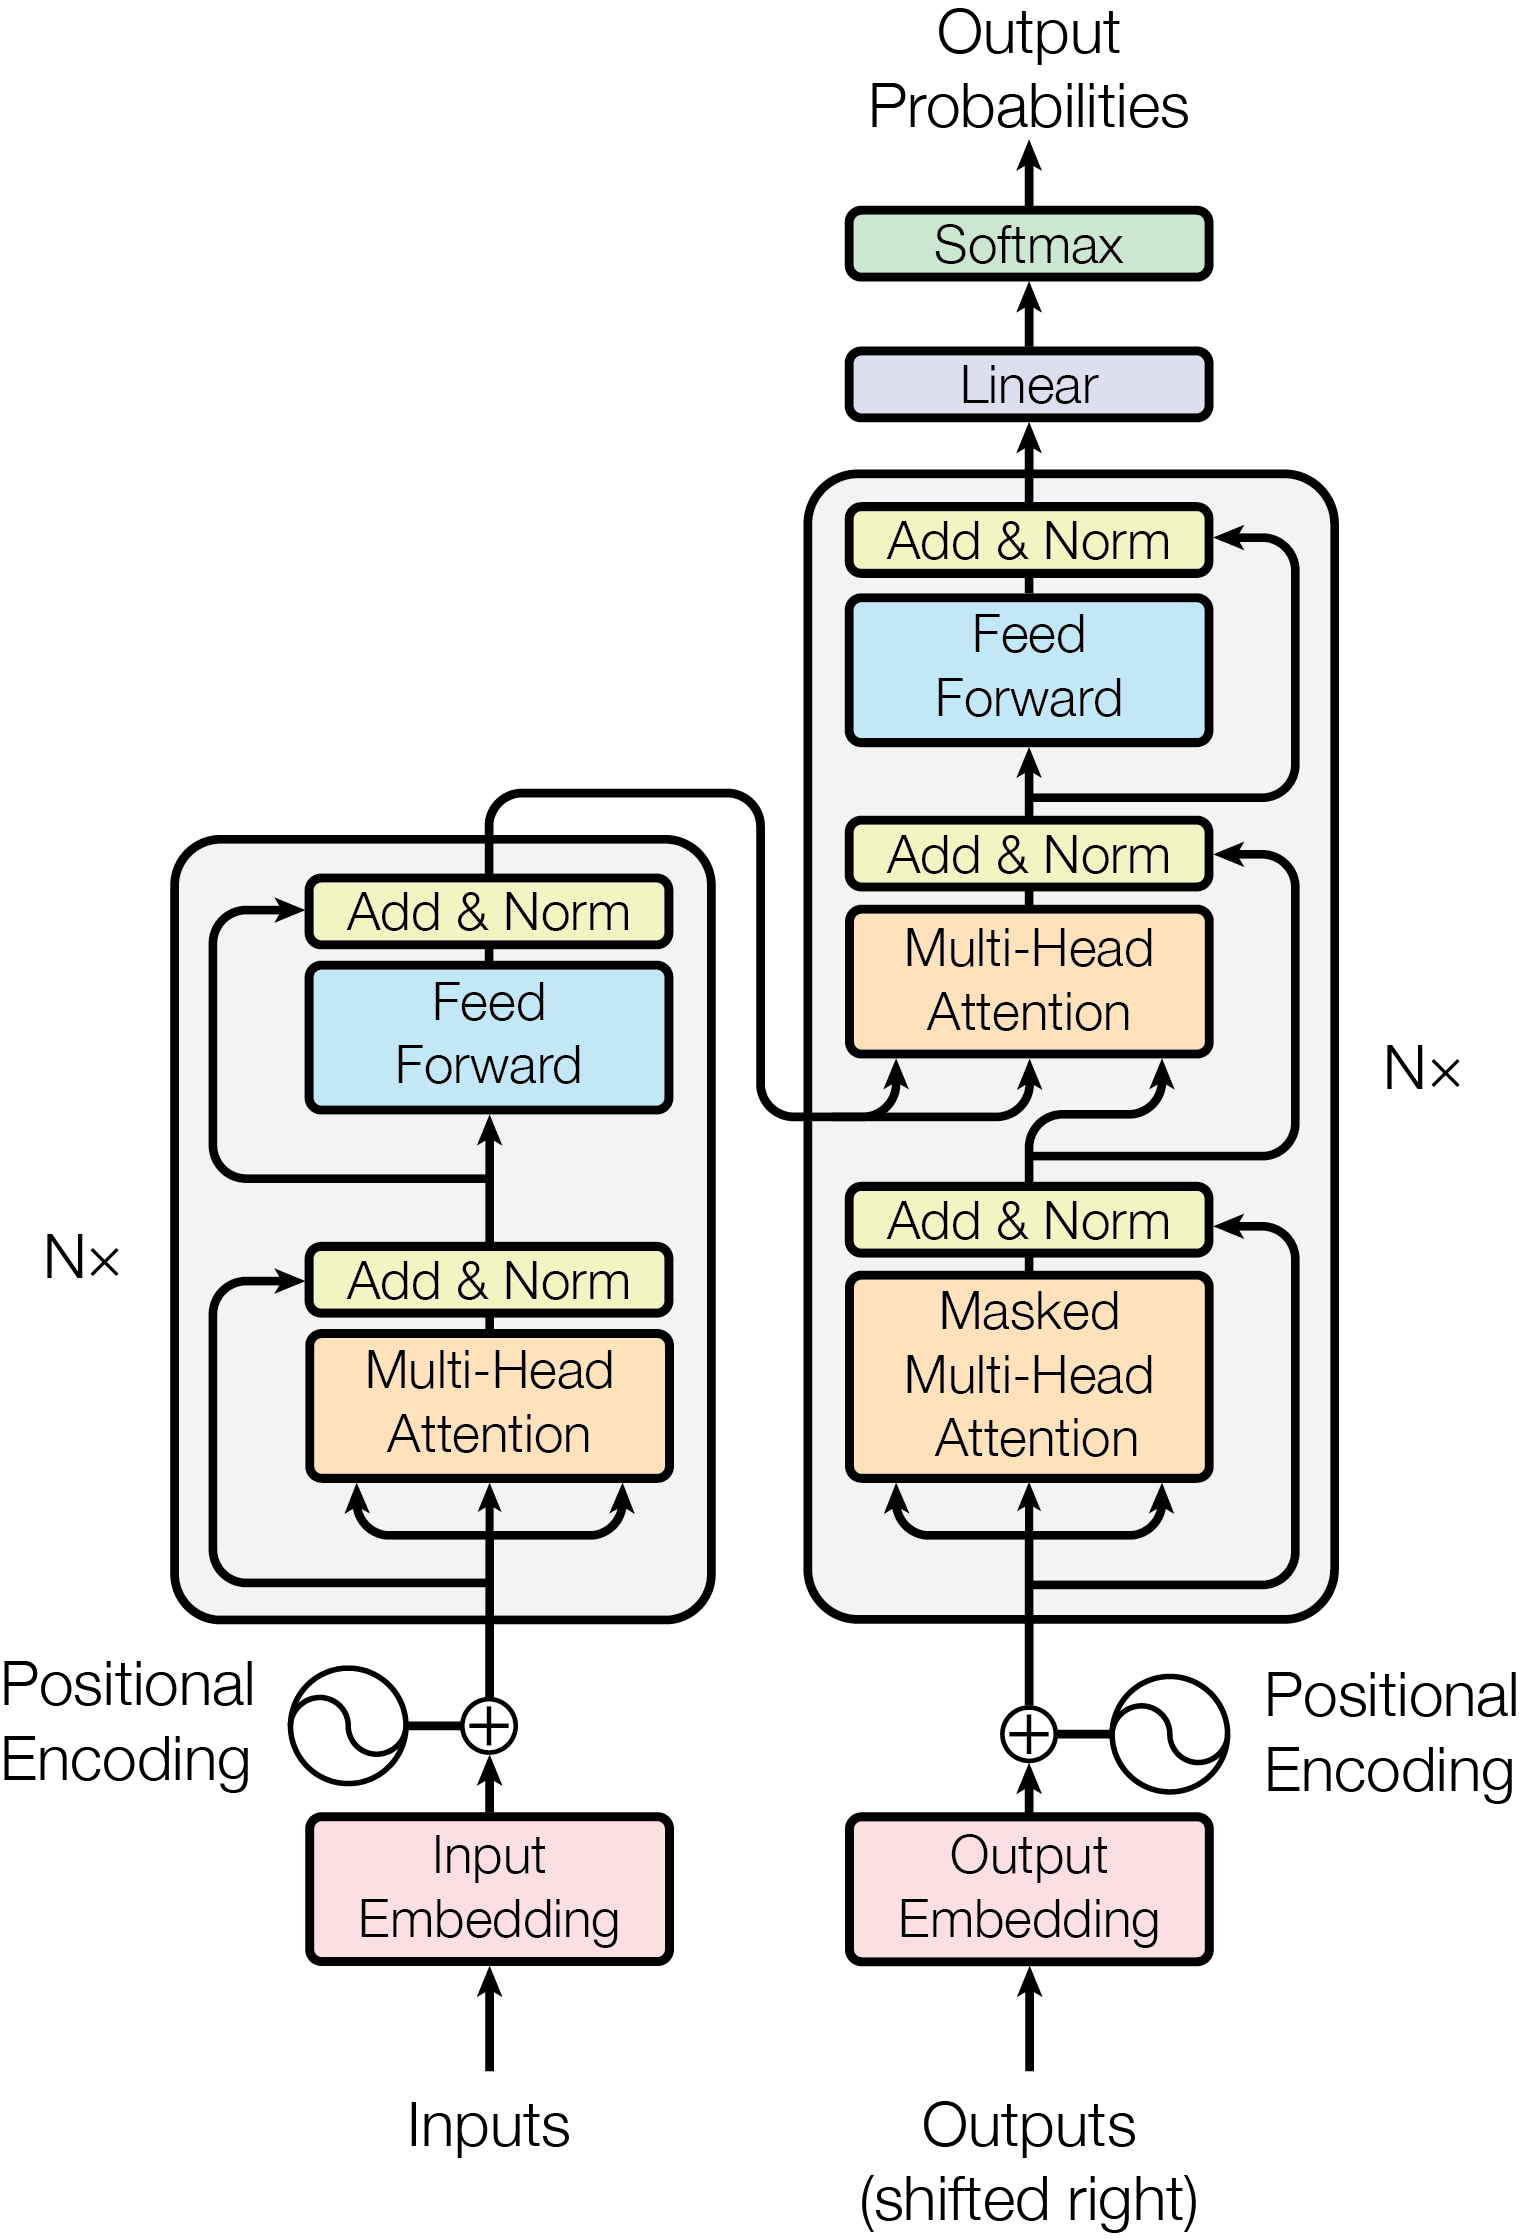
\includegraphics[width=0.5\linewidth]{chapter_3_theoretical_background/transformer.png}
	\caption{Overview of the Transformer architecture}
	Source: \textit{Attention Is All You Need} \cite{vaswani2017attention}
	\label{fig:chapter_3_theoretical_background/transformer}
\end{figure}

The Transformer architecture consists of an encoder and a decoder. The encoder takes as input a sequence of embeddings, such as word embeddings or character embeddings, and produces a sequence of hidden states that capture the information in the input sequence. The decoder takes as input the encoder hidden states and produces a sequence of output embeddings that represent the output sequence.

The encoder consists of multiple layers, each of which contains two sub-layers: a self-attention sub-layer and a feedforward sub-layer. In the self-attention sub-layer, the model computes a representation of each element in the input sequence by attending to all the other elements in the sequence. The feedforward sub-layer applies a pointwise fully connected layer to each position in the sequence independently and identically.

The decoder also consists of multiple layers, each of which contains three sub-layers: a self-attention sub-layer, a cross-attention sub-layer, and a feedforward sub-layer. In the self-attention sub-layer, the model attends to the previously generated output embeddings to compute the next output embedding. In the cross-attention sub-layer, the model attends to the encoder hidden states to incorporate information from the input sequence. The feedforward sub-layer applies a pointwise fully connected layer to each position in the sequence independently and identically.

The Transformer architecture uses residual connections and layer normalization to facilitate training of deep neural networks. Residual connections allow information to flow directly from one layer to another, bypassing the intermediate layers, which can help prevent the vanishing gradient problem. Layer normalization normalizes the input to each sub-layer to have zero mean and unit variance, which can help stabilize the training process.

Overall, the Transformer architecture has achieved state-of-the-art results on a wide range of natural language processing tasks, and its success has led to the development of a variety of transformer-based architectures, such as BERT, GPT, and T5.

\subsection{Graphs}
\label{subsec:3_graphs}

% https://arxiv.org/abs/2204.07697
% http://www.deepnlp.org/blog/latex-code-graph-neural-network
% https://towardsdatascience.com/graph-convolutional-networks-deep-99d7fee5706f
% https://www.datacamp.com/tutorial/comprehensive-introduction-graph-neural-networks-gnns-tutorial

A Graph is the type of data structure that contains nodes and edges. A node can be a person, place, or thing, and the edges define the relationship between nodes. The edges can be directed and undirected based on directional dependencies. 

Graphs are excellent in dealing with complex problems with relationships and interactions. They are used in pattern recognition, social networks analysis, recommendation systems, and semantic analysis. Creating graph-based solutions is a whole new field that offers rich insights into complex and interlinked datasets. 

Nevertheless, Graph-based data structures have drawbacks, and researchers must understand them before developing graph-based solutions.

\begin{itemize}
	\item A graph exists in non-euclidean space. It does not exist in 2D or 3D space, which makes it harder to interpret the data. To visualize the structure in 2D space, you must use various dimensionality reduction tools.
	\item Graphs are dynamic; they do not have a fixed form. There can be two visually different graphs, but they might have similar adjacency matrix representations. It makes it difficult for us to analyze data using traditional statistical tools.
	\item Large size and dimensionality will increase the graph's complexity for human interpretations. The dense structure with multiple nodes and thousands of edges is harder to understand and extract insights. 
\end{itemize}

\subsubsection{Graph Neural Networks}
\label{subsubsec:3_gnns}

GNNs are a class of neural networks that operate on graphs, which are collections of nodes and edges. A typical graph is represented by a set of node features, represented by a matrix $X \in \mathbb{R}^{N \times D}$, where $N$ is the number of nodes, and $D$ is the number of features associated with each node. Each node is also connected to other nodes via edges, which are represented by an adjacency matrix $A \in {0,1}^{N \times N}$, where $A_{ij} = 1$ if there is an edge between nodes $i$ and $j$, and $0$ otherwise.

\begin{itemize}
	\item A graph exists in non-euclidean space. It does not exist in 2D or 3D space, which makes it harder to interpret the data. To visualize the structure in 2D space, you must use various dimensionality reduction tools.
	\item Graphs are dynamic; they do not have a fixed form. There can be two visually different graphs, but they might have similar adjacency matrix representations. It makes it difficult for us to analyze data using traditional statistical tools.
	\item Large size and dimensionality will increase the graph's complexity for human interpretations. The dense structure with multiple nodes and thousands of edges is harder to understand and extract insights. 
\end{itemize}

The basic idea behind GNNs is to iteratively update the node representations using information from the graph neighborhood. Specifically, at each iteration, each node aggregates information from its neighbors, and the resulting aggregated representation is used to update the node's own representation. This process is typically repeated for multiple iterations until convergence. GNNs were introduced when Convolutional Neural Networks failed to achieve optimal results due to the arbitrary size of the graph and complex structure. 

One common way to implement this idea is to use the following update rule:

\begin{equation}
h_i^{(l+1)} = f(h_i^{(l)}, \sum_{j} A_{ij} h_j^{(l)})
\end{equation}

where $h_i^{(l)}$ is the representation of node $i$ at iteration $l$, $f$ is a non-linear activation function, and $\sum_{j} A_{ij} h_j^{(l)}$ is the sum of the representations of the neighbors of node $i$ at iteration $l$.

By stacking multiple layers of such updates, a GNN can learn increasingly complex representations of the graph.

There are several types of neural networks, such as:

\begin{itemize}
	\item Graph Auto-Encoder Networks, which learn graph representation using an encoder and attempt to reconstruct input graphs using a decoder. They are commonly used in link prediction as Auto-Encoders are good at dealing with class balance. 
	\item Recurrent Graph Neural Networks(RGNNs) are able to learn the best diffusion pattern, and they can handle multi-relational graphs where a single node has multiple relations. They are commonly used in generating text, machine translation, speech recognition or generating image descriptions
	\item Gated Graph Neural Networks (GGNNs) improve Recurrent Graph Neural Networks by adding a node, edge, and time gates on long-term dependencies, being the common uses similar to RGNNs.
\end{itemize}

Nevertheless, in this work we focus on a particular type of GNN, that is, Graph Convolutional Networks, which are the most common GNN type used in of \ac{MP} in the field of \ac{AD}.

\subsubsection{Graph Convolutional Networks}
\label{subsubsec:3_gcns}

The majority of GNNs are Graph Convolutional Networks (GCNs), which are a specific type of GNN that use convolutional operations to aggregate information from the graph neighborhood. GCNs were introduced when Convolutional Neural Networks failed to achieve optimal results due to the arbitrary size of the graph and complex structure. The basic idea behind GCNs is to treat the graph as a signal and use convolutional operations to extract features by inspecting neighboring nodes. GCNs aggregate node vectors, pass the result to the dense layer, and apply non-linearity using the activation function. 

\begin{figure}[h]
	\centering
	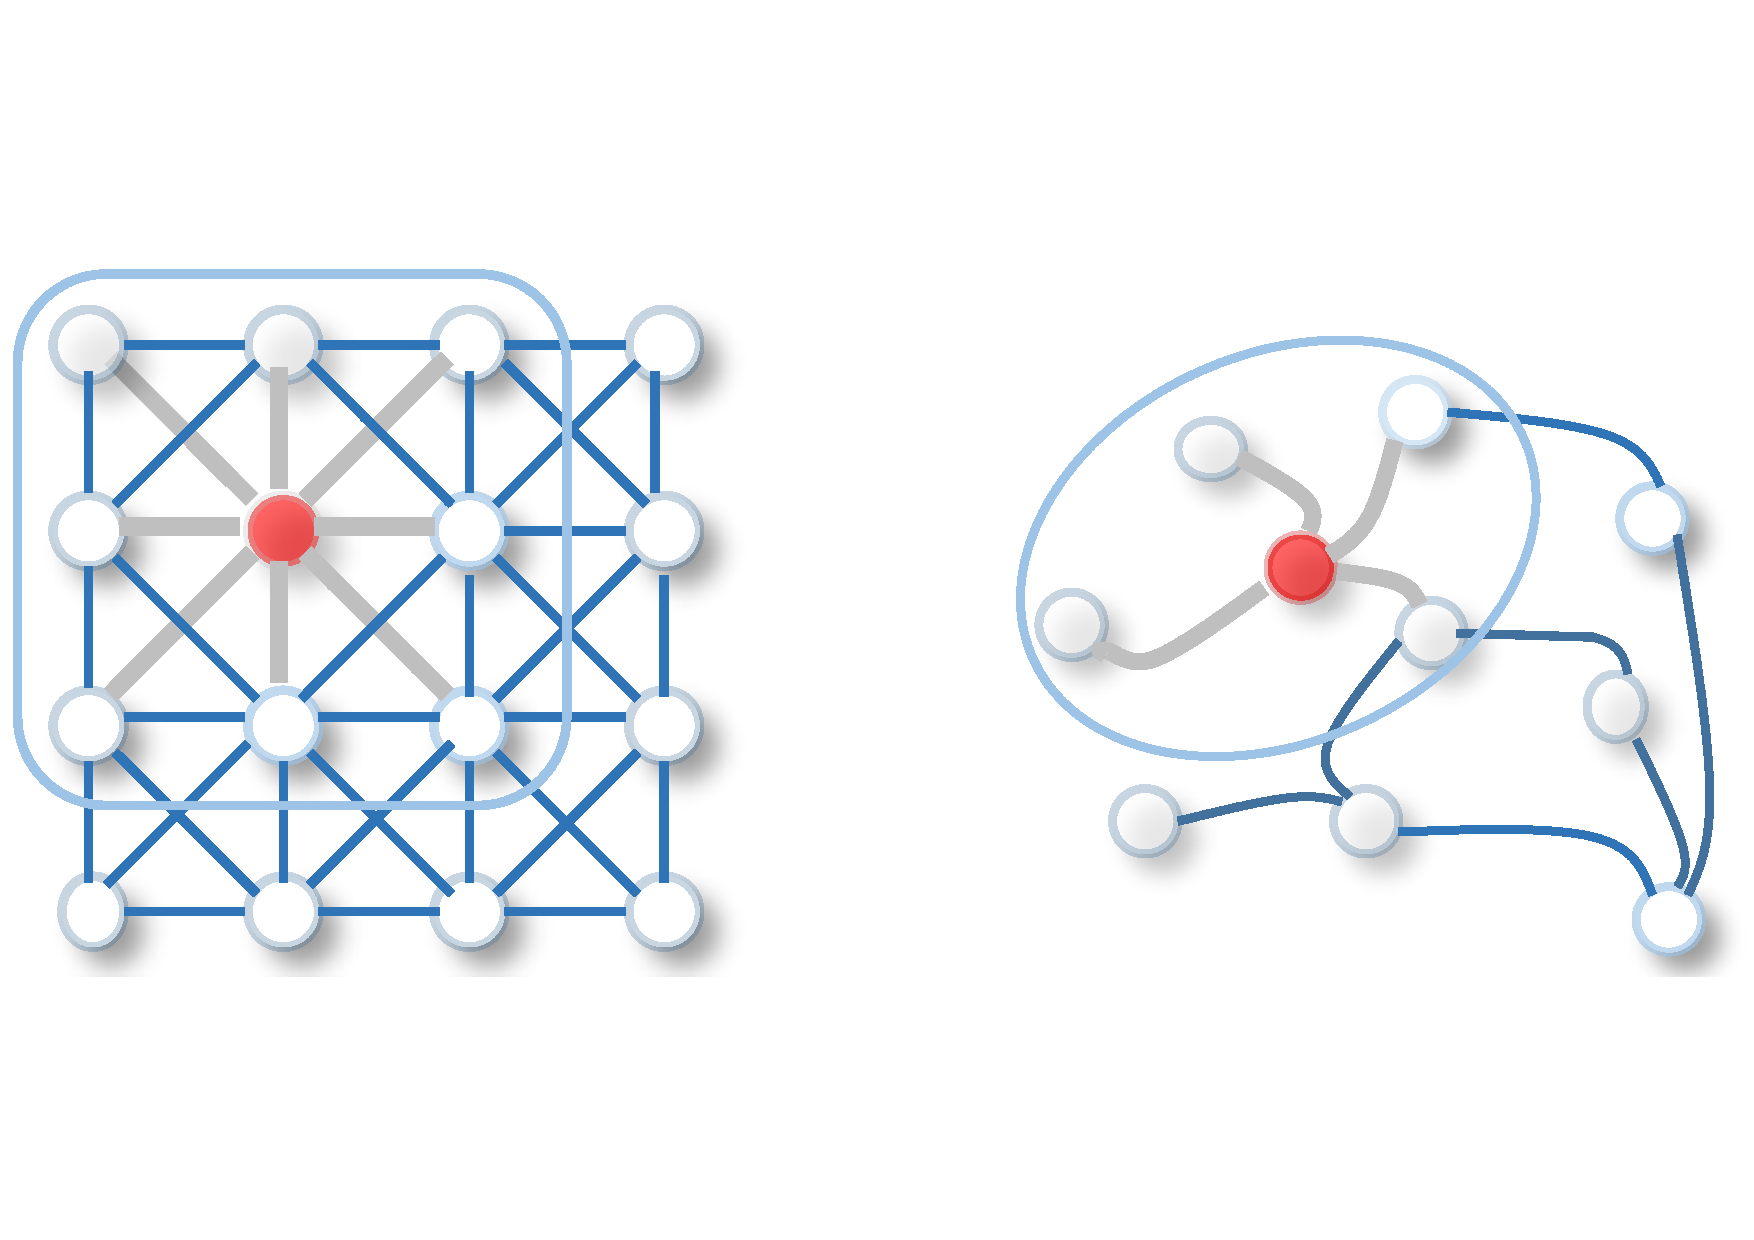
\includegraphics[width=0.6\linewidth]{chapter_3_theoretical_background/gcn_vs_cnn.pdf}
	\caption{Overview of the sliding kernel of a 2D-CNN vs GCN}
	Source: \textit{A comprehensive survey on graph neural networks} \cite{wu2020comprehensive}
	\label{fig:chapter_3_theoretical_background/gcn_vs_cnn}
\end{figure}

The major difference between GCN and CNN is that it is developed to work on non-euclidean data structures where the order of nodes and edges can vary, as it can be appreciated in Figure \ref{fig:chapter_3_theoretical_background/gcn_vs_cnn}. In 2D convolution, each pixel in an image is taken as a node where neighbours are determined by the filter size. The 2D convolution takes the weighted average of pixel values of the red node along with its neighbors. The neighbours of a node are ordered and have a fixed size. On the other hand, to get a hidden representation of a given node red, one simple solution of the graph convolutional operation is to take the average value of the node features of the red node along with its neighbors. Different from image data, the neighbors of a node are unordered and variable in size.

The convolution in GCN is the same as a convolution in convolutional neural networks. It multiplies neurons with weights (filters) to learn from data features. A convolutional operation on a graph is defined as:

\begin{equation}
H^{(l+1)} = \sigma(D^{-\frac{1}{2}} A D^{-\frac{1}{2}} H^{(l)} W^{(l)})
\end{equation}

where $H^{(l)}$ is the matrix of node representations at iteration $l$, $W^{(l)}$ is the weight matrix of the $l$-th layer, $A$ is the adjacency matrix of the graph, $D$ is the degree matrix of the graph, and $\sigma$ is a non-linear activation function.

The operation $D^{-\frac{1}{2}} A D^{-\frac{1}{2}}$ is a normalization step that scales the adjacency matrix by the inverse square root of the degree matrix. This normalization ensures that nodes with different degrees have similar influence in the convolutional operation. By stacking multiple layers of such convolutions, a GCN can learn increasingly complex features of the graph.

\subsection{Training}
\label{subsec:3_training}

Training is the process of iterating through a dataset to make the network learn the optimal mapping (combination of weights) from input to desired output in the data samples. In each iteration, a forward pass through the network is performed, computing the output of each layer until the end. This produces the output response of the network, which is then compared to a desired output with a defined Loss function (L). This function estimates the amount of error, which is back-propagated through the network to update its weights with the aim of minimizing the error. 

Regarding the supervised training paradigm, Backpropagation is an algorithm used for training artificial neural networks (ANNs) used to update the weights and biases of the neurons in the network based on the error between the predicted output and the actual output.

The backpropagation algorithm consists of two phases: the forward pass and the backward pass. During the forward pass, the input is fed into the network and propagated through the layers to obtain the predicted output. During the backward pass, the error between the predicted output and the actual output is computed and used to update the weights and biases of the neurons in the network.

The backpropagation algorithm is based on the chain rule of calculus, which allows the gradient of the loss function with respect to each weight and bias to be computed recursively from the output layer to the input layer of the network. The gradient descent algorithm is then used to update the weights and biases in the direction of the negative gradient of the loss function. In that sense, the main losses used in this work are described throughout the remaining content of this Chapter.

\subsubsection{Optimizer and learning rate}
\label{subsubsec:3_optimizer_and_lr}

There are several optimizers commonly used for training deep neural networks in the literature, such as Stochastic Gradient Descent (SGD) \cite{robbins1951stochastic}, Adagrad \cite{duchi2011adaptive}, Root Mean Square Propagation (RMSprop) \cite{zou2019sufficient} or Adadelta \cite{zeiler2012adadelta}. In this work we use one of the most extended, the ADAM \cite{kingma2014adam} optimizer. It is a popular optimization algorithm used in deep learning, particularly for training neural networks. It is an adaptive learning rate optimization algorithm that is well suited for large datasets and high-dimensional parameter spaces.

The basic idea behind ADAM is to compute adaptive learning rates for each parameter based on estimates of the first and second moments of the gradients. The algorithm computes a moving average of the gradients and their squared values, and uses these estimates to update the parameters with a learning rate that adapts to the local curvature of the loss function. The algorithm also includes bias-correction terms to ensure that the estimates are unbiased, especially in the early stages of training when the estimates are highly uncertain.

The update rule for ADAM can be expressed mathematically as follows:

\begin{equation}
\begin{split}
	m_t &= \beta_1 m_{t-1} + (1-\beta_1) g_t \\
	v_t &= \beta_2 v_{t-1} + (1-\beta_2) g_t^2 \\
	\hat{m}_t &= \frac{m_t}{1-\beta_1^t} \\
	\hat{v}t &= \frac{v_t}{1-\beta_2^t} \\
	\theta{t+1} &= \theta_t - \frac{\alpha}{\sqrt{\hat{v}_t}+\epsilon} \hat{m}_t
\end{split}
\end{equation}

where $\theta_t$ is the parameter vector at time step $t$, $g_t$ is the gradient vector, $m_t$ and $v_t$ are the first and second moment estimates at time step $t$, $\hat{m}_t$ and $\hat{v}_t$ are the bias-corrected moment estimates, $\alpha$ is the learning rate, $\beta_1$ and $\beta_2$ are the decay rates for the moment estimates, and $\epsilon$ is a small constant to prevent division by zero.

The algorithm starts with initializing $m_0$ and $v_0$ as zero vectors, and $\theta_0$ as the initial parameter vector. At each iteration, the gradient vector $g_t$ is computed using a batch of training data, and the moment estimates $m_t$ and $v_t$ are updated according to the first two lines of the update rule. The bias-corrected moment estimates $\hat{m}_t$ and $\hat{v}_t$ are then computed using the next two lines of the update rule. Finally, the parameter vector $\theta_t$ is updated using the last line of the update rule.

The hyperparameters $\alpha$, $\beta_1$, $\beta_2$, and $\epsilon$ can be tuned to optimize performance on a particular dataset and neural network architecture.

On the other hand, The learning rate is a key hyperparameter in the optimization process of machine learning algorithms, including optimizer updates like the ADAM optimizer. The learning rate controls the step size taken in the direction of the negative gradient during each iteration of the optimization process.

If the learning rate is too small, the optimization process will be slow and may get stuck in local minima. On the other hand, if the learning rate is too large, the optimization process may overshoot the minimum and oscillate back and forth, or even diverge.

In the context of the ADAM optimizer, the learning rate is used to adjust the size of the update step taken in the direction of the estimated gradient. The update step is multiplied by the learning rate, which determines the size of the step. A larger learning rate will result in larger update steps, and a smaller learning rate will result in smaller update steps.

In practice, the learning rate is usually set through a process called hyperparameter tuning, where different values of the learning rate are tried on a validation set to find the optimal value that results in the best performance of the model on the test set.

One common technique to adjust the learning rate during training is called learning rate scheduling. This involves decreasing the learning rate over time, often according to a predetermined schedule or based on the performance of the model on a validation set. This technique can help improve the convergence and stability of the optimization process, particularly in the later stages of training when the model is close to the optimal solution.

Overall, the learning rate plays a crucial role in the optimization process of machine learning algorithms, including optimizer updates like the ADAM optimizer. Selecting an appropriate learning rate is important for achieving fast and stable convergence to the optimal solution.

\subsubsection{Regression losses}
\label{subsec:3_regression_losses}

% https://blmoistawinde.github.io/ml_equations_latex/

A regression loss is a type of loss function used in regression problems to measure the difference between the predicted and true values of a continuous variable. In other words, it is a way to quantify how well a machine learning model is able to predict numerical values based on input data.

In regression problems, the goal is to learn a function that maps input features to output values. A regression loss is used to train the model by penalizing the difference between the predicted and true output values. The loss function is typically minimized during training, so that the model learns to make more accurate predictions. There are several types of regression loss functions, such as the Quantile loss, Log-Cosh or Mean Absolute Error (MAE). In this work we mainly focus on the Mean Square Error (MSE) and SmoothL1, also known as Huber loss.

\paragraph{Mean Square Error loss}
\label{par:3_mse_loss}

The Mean Squared Error (MSE) loss is a commonly used loss function in regression problems. It measures the average squared difference between the predicted and true values of a continuous variable. The MSE loss is given by:

\begin{equation}
	MSE(y, \hat{y}) = \frac{1}{n}\sum_{i=1}^{n}(y_i - \hat{y_i})^2
\end{equation}

where $y_i$ is the true value of the $i$-th data point, $\hat{y_i}$ is the predicted value, and $n$ is the number of data points.

The MSE loss penalizes large errors more strongly than small errors, since it uses the square of the difference between the predicted and true values. This makes it sensitive to outliers and can lead to overfitting if the data contains extreme values.

The MSE loss is used in many regression problems, such as linear regression, polynomial regression, and neural networks. It is often used as a performance metric to evaluate the quality of the model's predictions.

\paragraph{SmoothL1 loss}
\label{par:3_smoothL1_loss}

SmoothL1 loss, also known as Huber loss, is a loss function used in regression problems to measure the difference between the predicted and true values of a continuous variable. It is a variant of the L1 loss that is less sensitive to outliers and has a smooth gradient near zero.

The SmoothL1 loss function can be defined as follows:

\begin{equation}
\begin{split}
	L(y, \hat{y}) = \begin{cases}
		\frac{1}{2}(y - \hat{y})^2 & \text{if } |y - \hat{y}| < 1 \\
		|y - \hat{y}| - \frac{1}{2} & \text{otherwise} \
	\end{cases}
\end{split}
\end{equation}

where $y$ is the true value, $\hat{y}$ is the predicted value, and $|\cdot|$ represents the absolute value function.

The SmoothL1 loss function behaves like the L1 loss for small errors and like the L2 loss for large errors. Specifically, for errors smaller than 1, it uses the squared difference between the predicted and true values, which has a smooth gradient. For larger errors, it uses the absolute difference, which is less sensitive to outliers than the squared difference.

The SmoothL1 loss is used in regression problems when the data contains outliers or when the model needs to be less sensitive to large errors. It is commonly used in object detection and localization tasks, where the predicted bounding boxes can be highly sensitive to small changes in the input data.

\paragraph{Softmax loss}
\label{par:3_softmax_loss}

The softmax loss, also known as the cross-entropy loss, is a commonly used loss function in classification problems. It measures the difference between the predicted probability distribution and the true probability distribution of a categorical variable. The softmax loss is given by:

\begin{equation}
	CE(y, \hat{y}) = -\frac{1}{n}\sum_{i=1}^{n}\sum_{j=1}^{k} y_{i,j}\log(\hat{y_{i,j}})
\end{equation}

where $y_{i,j}$ is the true probability of the $i$-th data point belonging to class $j$, $\hat{y_{i,j}}$ is the predicted probability, $n$ is the number of data points, and $k$ is the number of classes.

The softmax function is applied to the output of the model to obtain a probability distribution over the classes. The predicted probability of class $j$ is given by:

\begin{equation}
	\hat{y_{i,j}} = \frac{e^{z_{i,j}}}{\sum_{l=1}^{k} e^{z_{i,l}}}
\end{equation}

where $z_{i,j}$ is the unnormalized score or logit for class $j$ of the $i$-th data point.

The softmax loss penalizes the model more heavily for predictions that are far from the true probabilities. It encourages the model to assign higher probabilities to the correct classes and lower probabilities to the incorrect classes.

The softmax loss is used in many classification problems, such as image classification, natural language processing, and speech recognition. It is often used as a performance metric to evaluate the quality of the model predictions.

\paragraph{Negative Log-Likelihood loss}
\label{par:3_NLL_loss}

Negative Log Likelihood (NLL) loss is a loss function commonly used in classification problems, particularly in deep learning models that output probabilities for each class. It is a type of maximum likelihood estimation (MLE) loss, which means it attempts to maximize the likelihood of the predicted probabilities given the true labels.

The NLL loss function can be defined as follows:

\begin{equation}
	L(y_i, \hat{y_i}) = -\log(\hat{y_{i,y_i}})
\end{equation}

where $y_i$ is the true label of the $i$-th data point, $\hat{y_i}$ is the predicted probability distribution for that point, and $\hat{y_{i,y_i}}$ is the predicted probability for the true label.

The NLL loss penalizes the model for assigning low probabilities to the true label, while rewarding it for assigning high probabilities. It is a logarithmic loss function, which means that the penalty for low probabilities increases exponentially as the predicted probability approaches zero.

The NLL loss is used in classification problems because it provides a gradient that can be used to update the model parameters during training, in order to improve the accuracy of the predicted probabilities. It is commonly used in conjunction with softmax activation function, which ensures that the predicted probabilities sum to one across all classes.

\paragraph{Winner-Takes-All loss}
\label{par:3_WTA_loss}

Winner-Takes-All (WTA) loss is a loss function used in clustering problems, particularly in competitive learning models. It is a type of unsupervised learning, which means that it does not require labeled data for training.

The WTA loss function can be defined as follows:

\begin{equation}
\begin{split}
	L(y_i, f(x_i)) = \begin{cases}
		0 & \text{if } y_i = \arg\max_j f_j(x_i) \\
		1 & \text{otherwise} \
	\end{cases}
\end{split}
\end{equation}

where $y_i$ is the true cluster of the $i$-th data point, $f_j(x_i)$ is the activation of the $j$-th neuron in the output layer for that point, and $\arg\max_j f_j(x_i)$ is the index of the neuron with the highest activation.

The WTA loss function penalizes the model for assigning a data point to the wrong cluster. It works by forcing each neuron in the output layer to specialize in a particular cluster, such that the neuron with the highest activation for a given point corresponds to the true cluster of that point.

The WTA loss is used in clustering problems because it encourages the model to learn a set of representative clusters that capture the structure of the data, without requiring any prior knowledge of the true labels. It is commonly used in conjunction with competitive learning algorithms, such as self-organizing maps (SOMs), that use local competition between neurons to learn a topology-preserving mapping from the input space to the output space.

\paragraph{Hinge loss}
\label{par:3_hinge_loss}

Hinge loss is a loss function used in classification problems, particularly in support vector machines (SVMs). It is a type of max-margin loss, which means it attempts to maximize the margin between the decision boundary and the data points.

The hinge loss function can be defined as follows:

\begin{equation}
	L(y_i, f(x_i)) = \max(0, 1 - y_i f(x_i))
\end{equation}

where $y_i$ is the true label of the $i$-th data point, $f(x_i)$ is the predicted score for that point, and $1$ is a margin hyperparameter that determines the width of the margin.

If $y_i f(x_i) \geq 1$, then the point is correctly classified and the loss is zero. If $y_i f(x_i) < 1$, then the point is misclassified and the loss is proportional to the distance between the predicted score and the correct score. The loss function penalizes misclassifications linearly, with a slope of -1 for negative misclassifications and 0 for positive misclassifications.

The hinge loss is used in SVMs because it encourages the model to find a decision boundary that maximizes the margin between the classes, while still correctly classifying the data points. This results in a more robust and generalizable model.

\subsubsection{Regularization techniques}
\label{subsubsec:3_regularization}

Regularization techniques in deep learning are used to prevent overfitting and improve the generalization performance of a model. Overfitting occurs when a model fits the training data too closely and captures noise or irrelevant patterns, resulting in poor performance on new, unseen data. Here are some commonly used regularization techniques in deep learning:

L1 and L2 regularization: L1 and L2 regularization are two popular regularization techniques that add a penalty term to the loss function during training. L1 regularization adds the sum of the absolute values of the weights to the loss function, while L2 regularization adds the sum of the squares of the weights. This encourages the model to learn simpler and more generalizable representations by shrinking the weights towards zero.

Dropout: Dropout is a regularization technique that randomly drops out some units (neurons) in a layer during training. This forces the remaining units to learn more robust and diverse representations that generalize better to new data. Dropout has been shown to be effective in reducing overfitting, particularly in deep neural networks with many layers.

Data augmentation: Data augmentation is a technique that artificially increases the size of the training set by generating new examples from existing ones. This can be done by applying transformations such as rotations, translations, flips, or adding noise to the input data. Data augmentation can help reduce overfitting by increasing the diversity of the training data and improving the generalization performance of the model.

Early stopping: Early stopping is a technique that monitors the performance of the model on a validation set during training and stops the training process when the performance starts to degrade. This prevents the model from overfitting to the training data and allows it to generalize better to new data.

Batch normalization: Batch normalization is a technique that normalizes the activations of a layer by subtracting the batch mean and dividing by the batch standard deviation. This helps stabilize the distribution of the activations and reduces the internal covariate shift, which can improve the training process and reduce overfitting.

Weight decay: Weight decay is a technique that adds a penalty term to the loss function during training, similar to L2 regularization. The penalty term is proportional to the square of the weights, and it encourages the model to learn smaller and simpler weights, which can reduce overfitting.

These are some of the commonly used regularization techniques in deep learning. They can be combined and tuned to improve the performance of a model on a specific task and dataset.

Moreover, another interesting technique to help the model improve during training is hard-mining. Hard-mining is a technique in deep learning used to improve the training of a model by focusing on the samples that are most difficult to classify correctly.

During training, the model makes predictions on a batch of training data, and the loss function is computed based on the difference between the predicted values and the true values. In hard-mining, the training samples that contribute the most to the loss function are identified, and these samples are given more importance during training.

The idea behind hard-mining is that by focusing on the difficult samples, the model is forced to learn more discriminative features that can better distinguish between the different classes. This can lead to better generalization performance and improved accuracy on the test data.

There are several ways to implement hard-mining in deep learning, including:

\begin{itemize}
	\item Hard negative mining involves selecting the training samples that are misclassified with the highest confidence by the model and including them in the next batch of training data. By focusing on the difficult negative samples, the model can learn to better distinguish between the different classes and reduce the number of false negatives.
	
	\item Hard positive mining involves selecting the training samples that are misclassified with the lowest confidence by the model and including them in the next batch of training data. By focusing on the difficult positive samples, the model can learn to better distinguish between the different classes and reduce the number of false positives.
	
	\item Curriculum learning involves gradually increasing the difficulty of the training data over time. The model is first trained on easy samples and then gradually exposed to more difficult samples. This can help the model learn more robust and generalizable features by gradually increasing the complexity of the training data.
	
	\item Overall, hard-mining is a useful technique in deep learning for improving the training of a model by focusing on the difficult samples. By incorporating hard-mining into the training process, the model can learn more discriminative features and improve its generalization performance on new, unseen data.
\end{itemize}

\section{Summary}
\label{sec:3_summary}

In this chapter, the mathematical background of various physics-based and \ac{DL}-based techniques used for \ac{MP} models is thoroughly examined. The chapter aims to provide a comprehensive understanding of these methods and their applications in the field of motion prediction.

The chapter begins by introducing the physics-based techniques, starting with the Kalman Filter. The Kalman Filter is a recursive algorithm used to estimate the state of a dynamic system by incorporating noisy measurements. Its mathematical foundation, including the state-space model and the prediction and update steps, is discussed in detail. Next, the Hungarian Algorithm is presented, which is a combinatorial optimization algorithm used for data association in multiple object tracking. The chapter delves into the mathematical formulation of the Hungarian Algorithm and how it can be applied to motion prediction tasks.

Moving on to the physics-based models, the chapter explores the \ac{CTRV} and \ac{CTRA} models. These models are widely used for trajectory prediction and capture the motion dynamics of objects by considering their position, velocity, and acceleration. The mathematical equations for these models are examined, highlighting how they can be utilized to predict future motion paths.

The chapter then transitions to deep learning-based techniques, which have gained significant attention in recent years due to their ability to capture complex patterns and dependencies in data. Several models are discussed in detail, starting with the 1D-Convolutional Neural Network (CNN). The mathematical architecture of the 1D-CNN is explained, emphasizing its ability to extract spatial and temporal features from sequential data for motion prediction.

Next, the \ac{LSTM} model is introduced, which is a type of recurrent neural network (RNN) specifically designed to handle sequence data. The chapter provides an overview of the \ac{LSTM} architecture, including its memory cell and gate mechanisms, which enable it to capture long-term dependencies and predict future motion accurately.

The chapter then explores \acp{GAN} and their application in motion prediction. \acp{GAN} consist of a generator and discriminator network that compete against each other, resulting in the generation of realistic and coherent motion trajectories. The mathematical formulation of \acp{GAN} and their training process are examined in detail.

Furthermore, the Graph Convolutional Network (GCN) is discussed, which is a deep learning model capable of operating on graph-structured data. The chapter explains how GCNs can be used to represent and predict motion patterns in scenarios where objects interact with each other.

Finally, the Attention mechanism is examined, which is a component commonly integrated into deep learning models to focus on relevant parts of the input data. The chapter explores the mathematical formulation of the Attention mechanism and its application in motion prediction models, highlighting its ability to assign different weights to different input features based on their relevance.

Overall, this chapter provides a comprehensive overview of the mathematical foundations of various physics-based and deep learning-based techniques used in motion prediction models. By understanding the underlying principles and equations of these models, researchers and practitioners can gain a deep understanding of their capabilities and make informed decisions regarding their application in different scenarios.
%%%%%%%%%%%%%%%%%%%%%%%%%%%%%%%%%%%%%%%%%%%%%%%%%%%%%%%%%%%%%%%%%%%%%%%%%%% 
% 
% Generic template for TFC/TFM/TFG/Tesis
% 
% By:
% + Javier Macías-Guarasa. 
% Departamento de Electrónica
% Universidad de Alcalá
% + Roberto Barra-Chicote. 
% Departamento de Ingeniería Electrónica
% Universidad Politécnica de Madrid   
% 
% Based on original sources by Roberto Barra, Manuel Ocaña, Jesús Nuevo,
% Pedro Revenga, Fernando Herránz and Noelia Hernández. Thanks a lot to
% all of them, and to the many anonymous contributors found (thanks to
% google) that provided help in setting all this up.
% 
% See also the additionalContributors.txt file to check the name of
% additional contributors to this work.
% 
% If you think you can add pieces of relevant/useful examples,
% improvements, please contact us at (macias@depeca.uah.es)
% 
% You can freely use this template and please contribute with
% comments or suggestions!!!
% 
%%%%%%%%%%%%%%%%%%%%%%%%%%%%%%%%%%%%%%%%%%%%%%%%%%%%%%%%%%%%%%%%%%%%%%%%%%% 

\chapter{SmartMOT: Exploiting the fusion of HD maps and Multi-Object Tracking for Real-Time scene understanding}
\label{cha:smartmot_exploiting_the_fusion_of_hdmaps_and_mot}

\begin{FraseCelebre}
	\begin{Frase}
		¡Avanzad, sin temor a la oscuridad! \\
		¡Luchad! ¡Luchad! ¡Luchad jinetes de Théoden! \\
		¡Caerán las lanzas, se quebrarán los escudos,  \\
		aún restará la espada! \\
		¡Rojo será el día hasta el meced del sol! \\
		¡Cabalgad! ¡Cabalgad! \\
		¡Cabalgad a la desolación y al fin del mundo! \\
		¡Muerte! ¡Muerte! ¡Muerte! ¡Adelante Eorlingas!
	\end{Frase}
	\begin{Fuente}
		Discurso de Theoden, Rey de Rohan \\
		Batalla de los Campos de Pelennor \\
		El Señor de los Anillos: El Retorno del Rey
	\end{Fuente}
\end{FraseCelebre}

\section{Introduction}
\label{sec:4_introduction}

In order to achieve a reliable navigation, \acfp{ADS} must perform safe driving behaviours following conventional traffic rules. One of the key concepts when developing safe \acp{ADS} is the perception of the environment. Furthermore, the reliability of the \ac{DM} and local planning modules lies on the performance of the environment detector and its ability to predict future situations. In that sense, a real-time \ac{MOT} system, which goal is to associate detections (usually in the 3D or \ac{BEV} space) in a sequence, is essential for \ac{AD} applications, representing in most cases the preliminary stage before predicting the subsequent future trajectories of these obstacles in the scene, giving the car a valuable reaction time to avoid critical situations or to anticipate its behaviour for the corresponding traffic scenario. The improvements in object detection in the last years have allowed the research community, specially those groups related to \ac{AD}, to focus on \ac{MOT} techniques as a preliminary stage before implementing \ac{MP}, yielding higher accuracy at the cost of computational complexity, making its use prohibitive in real-time systems. 

\ac{MOT} systems aim to estimate the orientation, location and scale of all the objects in the environment over time. While object detection only captures the information of the environment in a single frame, a tracking system must take temporal information into account, filtering outliers (\aka \ false positives) in consecutive detections and being robust to partial or full occlusions. When travelling throughout a route programmed by the path-planner, the vehicle may detect an undetermined number of unforeseen objects over which the \ac{MOT} module should consider only the most relevant from a safety point of view (such as pedestrians, cyclists or cars) to predict and monitor their trajectories. Then, the vehicle can use the evolution of the scene over time to infer driving behaviour and motion patters for improved \ac{MP}.

Most \ac{MOT} approaches \cite{weng20203d, chiu2021probabilistic} model the state of each obstacle with its 3D position, scale, orientation and their corresponding linear and angular velocity. These approaches introduce an unnecessary complexity and computational cost to the system, since most traffic scenes can be described in terms of 2D position, angular and linear velocity, apart from the orientation and scale of the resulting bounding box, that is, a \ac{BEV} perspective, as depicted in Figure \ref{fig:chapter_4_SmartMOT/ITSC_2020_coordinates_conversion}. 

\begin{figure}[h]
	\centering
	\captionsetup{justification=justified}
	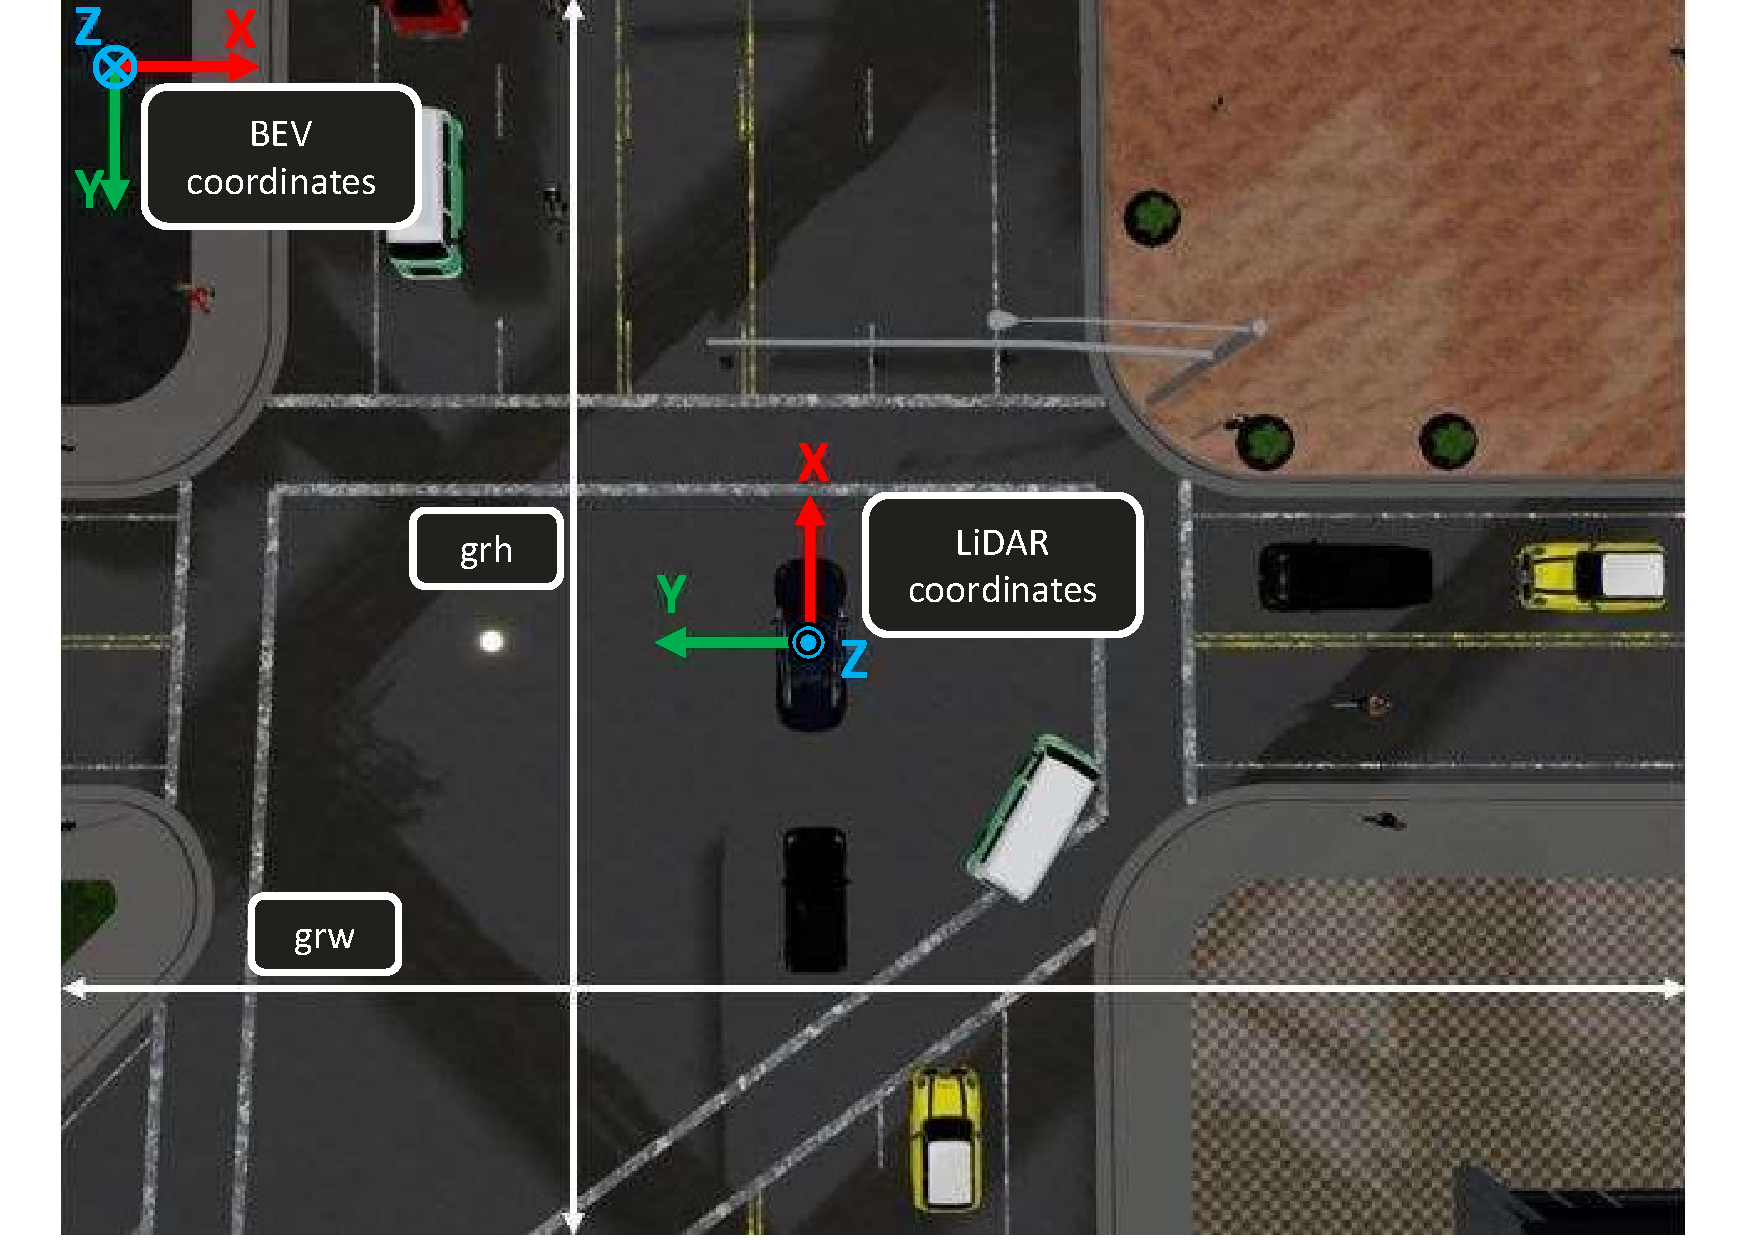
\includegraphics[trim=0 0 0 1cm, width=0.8\textwidth]{chapter_4_SmartMOT/ITSC_2020_coordinates_conversion.pdf}
	\caption[LiDAR to BEV (Bird's Eye View) coordinates transformation illustrated in the CARLA simulator]{LiDAR to BEV (Bird's Eye View) coordinates transformation illustrated in the CARLA simulator. \textit{grw} and \textit{grh} stands for the height and width of our real-world grid respectively.}
	\label{fig:chapter_4_SmartMOT/ITSC_2020_coordinates_conversion}
\end{figure}

This Chapter summarizes the SmartMOT pipeline and the experimental results obtained with our proposal. The work in this Chapter was partially published in the following conference paper \cite{gomez2021smartmot}: "SmartMOT: exploiting the fusion of \acp{HDmap} and multi-object tracking for real-time scene understanding in intelligent vehicles applications", 2021 IEEE Intelligent Vehicles Symposium (IV), p. 710-715. We make the following contributions:

\begin{enumerate}
	
	\item We propose SmartMOT, an \href{https://github.com/Cram3r95/SmartMOT}{open-source} \footnote{https://github.com/Cram3r95/SmartMOT} simple-yet-accurate pipeline to perform real-time \ac{MOT} and physics-based uni-modal \ac{MP}.
	
	\item A Monitored Lanes-based Attention Module is proposed to extract monitored lanes around the ego-vehicle (including standard lanes and intersections) and filter non-relevant obstacles. Then, the ego-vehicle will track only those agents that are in the monitored area.
	
	\item We study the \ac{MOT} in the KITTI \ac{MOT} dataset and in data captured by our real-world vehicle, as well as the influence of the map monitor to reduce the inference time of the pipeline in the \ac{CARLA} simulator, with the ultimate goal of achieving real-time uni-modal prediction based on kinematics.
	
\end{enumerate}

\section{SmartMOT pipeline}
\label{sec:4_smartmot}

In order to solve the problem of monitoring the relevant objects around the ego-vehicle in an efficient way, we propose SmartMOT \cite{gomez2021smartmot}, a simple-yet-accurate tracking-by-detection pipeline which consists of a combination of traditional techniques such as the \ac{KF} \cite{kalman1960new} and \ac{HA} \cite{kuhn1955hungarian} for state estimation and data association respectively. Moreover, we incorporate \ac{HDmap} information, in addition to the ego-vehicle status, so as to enhance the efficiency and reliability of the tracking system and subsequent predictions, as observed in Figure \ref{fig:chapter_4_SmartMOT/IV_2021}. 

The SmartMOT pipeline (Figure \ref{fig:chapter_4_SmartMOT/IV_2021}) is made up by: (1) 3D object detection module that returns the bounding boxes, (2) Monitored Area to filter non-relevant objects, \eg \ the \acfp{VRU} that are inside the sidewalk far away the road or the vehicles that are located in a lane in which lane change is not allowed, (3) \acf{BEV} \acf{KF} that predicts the object state from the current frame and updates the object state based on the detected bounding boxes at current frame, (4) \acf{HA}, which associates the current trackers with new detections, (5) Birth and Death memory that deals with the disappeared trajectories (unmatched trajectories exceeding ${age_{max}}$ frames) and the newly appeared trajectories (matched trajectories exceeding ${f_{min}}$ frames) and (6) \ac{CTRV} model which performs short-term physics-based \ac{MP} of the updated trackers information using both the linear and angular velocity information. As observed, except for the pre-trained object detector module, our \ac{MOT} system does not need any training and can be directly used for inference.

\begin{figure}[h]
	\centering
	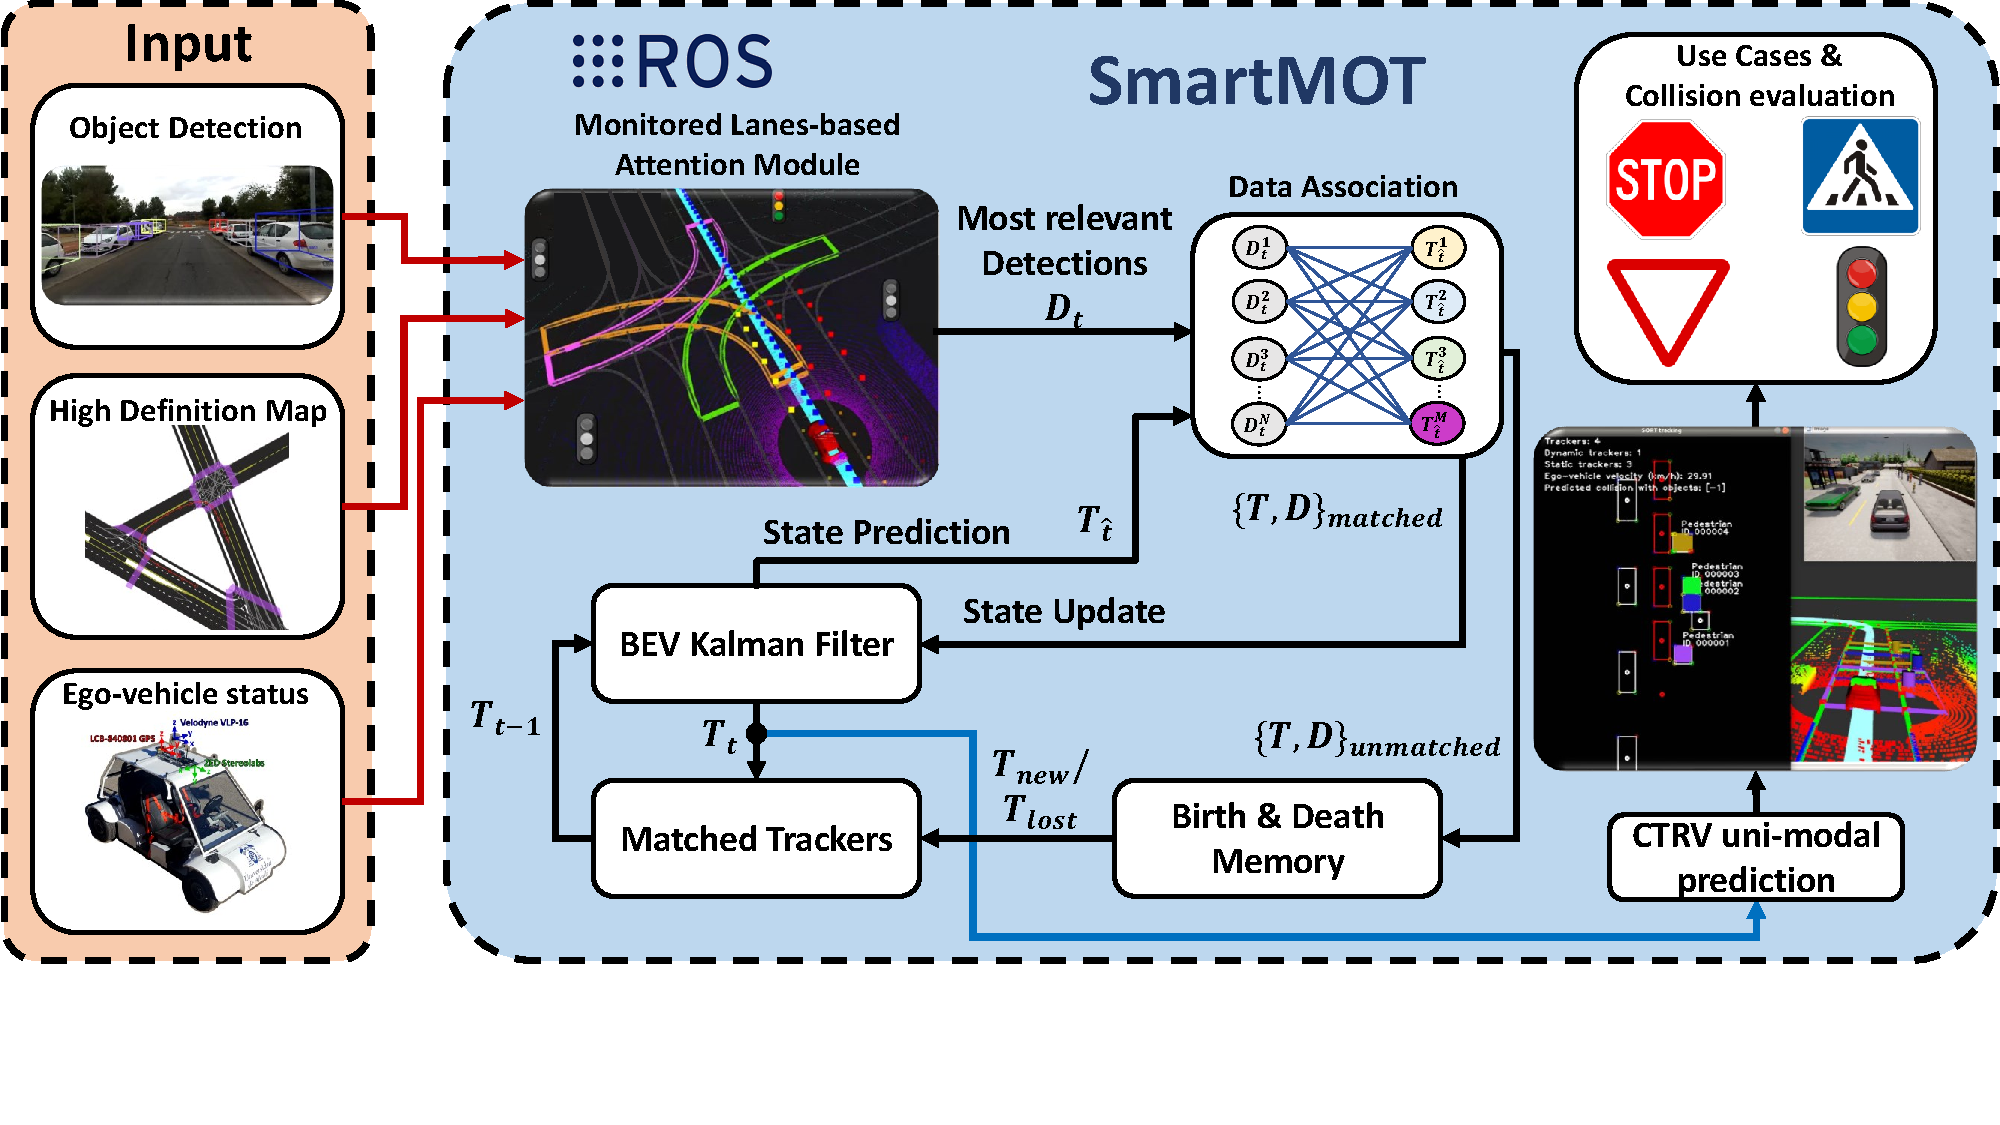
\includegraphics[trim=0cm 3cm 0cm 0cm, width=\textwidth]{chapter_4_SmartMOT/IV_2021.pdf}
	\captionsetup{justification=justified}
	\caption[SmartMOT pipeline for Multiple-Object Tracking and Short-Term Motion Prediction]{SmartMOT pipeline for Multiple-Object Tracking and Short-Term Motion Prediction. It can be observed that we use as inputs the obstacles 360\degree~detected in the environment, the HD map information and ego-vehicle status. Only those agents that are relevant are tracked, predicted and evaluated in the corresponding use cases.}
	% $\textbf{SmartMOT pipeline}$: $\textbf{(1)}$ The object detection module, mapping layer and localization layer provide the 3D bounding boxes at frame \textit{t}, monitored lanes and ego-vehicle status data respectively; $\textbf{(2)}$ A Monitored Lanes-based Attention Module filters the non-relevant traffic participants and transforms the remaining into the \ac{BEV} image plane; $\textbf{(3)}$ A \ac{BEV} Kalman Filter predicts the state of trajectories in frame \textit{t-1} to current frame \textit{\^{t}} throughout the prediction step; $\textbf{(4)}$ detections at frame \textit{t} and predicted trajectories at \textit{\^{t}} are matched using the Khun-Munkres (\aka \ Hungarian) algorithm; $\textbf{(5)}$ matched trajectories are updated based on their corresponding matched detections and every tracker is evaluated again based on its particular monitorized area, to obtain updated trajectories at frame \textit{{t}}; $\textbf{(6)}$ Unmatched trajectories and detections are used to delete disappeared trajectories or create new ones respectively; $\textbf{(7)}$ Updated trackers at frame \textit{{t}} are predicted using a CTRV model and then evaluated using the monitors module.
	\label{fig:chapter_4_SmartMOT/IV_2021}
\end{figure}

\subsection{3D Object Detection}
\label{subsec:4_smartmot_detection}

The first step our \ac{MOT} algorithm must carry out is to detect the obstacles in the environment around the ego-vehicle. Since this thesis does not focus on the object detection stage of the perception layer, experiments to integrate the object detection and monitored area are conducted in the \ac{CARLA} assuming ground-truth detection including Gaussian noise in the \textit{x,y,z}-axis to simulate real-world detections. Then, at a given frame \textit{t}, the detections provided by the object detection module are given in the following form:

\begin{equation}
	\label{eq:4_smartmot_detection}
	D_{t} =[D_{t}^{1},D_{t}^{2}, ...,D_{t}^{N}]
\end{equation}

Where \textit{N} is the number of detected 3D bounding boxes at a given frame and threshold. At this point, instead of using all the 3D information of the object \cite{chiu2021probabilistic, weng20203d}, we take its projection on the floor plane (\ac{BEV} information), to reduce the complexity and computational cost of the tracking stage, specially in those urban scenarios full of vehicles, based on the assumption that the height (\textit{z}) dimension is not as important as other coordinates (\textit{x}-axis, \textit{y}-axis) in a context of self-driving navigation. Detected 3D bounding boxes are referred to the \ac{LiDAR} coordinate system. A grid is applied to establish a relation between real-world and image dimensions to discretize the possible positions of the detected bounding boxes and decrease the complexity and computational cost of the tracking module. 

Conducting \ac{MOT} in the discrete space \ac{BEV} using pixels instead of 3D real-world units using meters offers several advantages in certain applications and scenarios. Some of these advantages include:

\begin{itemize}
	
	\item \textbf{Computational Efficiency}: Representing the 3D scene in the \ac{BEV} space using pixels allows for faster and more efficient processing, with reduced memory requirements. Working with pixels reduces the complexity of computations compared to using real-world units, as it involves simple 2D operations rather than more complex 3D calculations which often involve larger floating-point values, particularly in terms of the \ac{KF} update/predict transitions or 3D-\ac{IOU} as metric in the affinity matrix of the \acf{HA}.
	
	\item \textbf{Simplified Data Representation}: In the \ac{BEV} space, the environment is represented as a 2D image, which can be easily handled by standard computer vision techniques. This simplification makes it easier to implement and integrate \ac{MOT} algorithms with existing image processing pipelines.

	\item \textbf{Sensor Independence}: The \ac{BEV} representation is sensor agnostic, meaning it can be easily adapted to work with various sensor types, such as \ac{LiDAR} (present case) but also camera or \ac{RADAR}, without the need for sensor-specific calibration or transformations.
	
	\item \textbf{Occlusion Handling}: In the \ac{BEV}, occlusions between objects can be more straightforward to handle. Occluded objects may still be partially visible in the image, and tracking algorithms can take advantage of this partial information to maintain better tracking continuity.
	
	\item \textbf{Top-Down Contextual Information}: By observing the scene from a top-down perspective, the algorithm can gain a holistic view of the environment and utilize higher-level contextual information, such as road layout, lanes, and traffic rules, which can aid in improving tracking accuracy.
	
	\item \textbf{Object Shape Normalization}: When objects are projected onto the \ac{BEV}, they are often represented by simple shapes (\eg \ rectangles) rather than complex 3D shapes. This simplification can facilitate object association and matching across frames (as proposed in the present Chapter).

\end{itemize}

Nevertheless, despite these advantages, it is essential to note that using pixels in the \ac{BEV} space may introduce limitations. For instance, the resolution and accuracy of the tracking might be constrained by the pixel grid size. In that sense, our grid is featured by a rectangle, whose center is located at the \ac{LiDAR} position on the vehicle, where $\textit{grw}$ and $\textit{grh}$ represent the width and height of the grid in \ac{LiDAR} coordinates $\textit{m}$ (meters) respectively, as depicted in Figure \ref{fig:chapter_4_SmartMOT/ITSC_2020_coordinates_conversion}. Then, each detection in Equation \ref{eq:4_smartmot_detection_tuple} is represented as the tuple:

\begin{equation}
	\label{eq:4_smartmot_detection_tuple}
	D_{t}^{i} = [x_{m},y_{m},w_{m},l_{m},\theta,type,score]
\end{equation}

Where $\textit{$x_{m},y_{m}$}$ correspond to the object centroid in \ac{LiDAR} coordinates ($\textit{m}$), $\textit{$w_{m}$}$ and $\textit{$l_{m}$}$ correspond to the width and length of the object respectively ($\textit{m}$), $\theta$ its orientation angle around the \ac{LiDAR} $z$-axis, object type and detection confidence. Figure \ref{fig:chapter_4_SmartMOT/ITSC_2020_coordinates_conversion} illustrates the transformation from the source coordinate system (\ac{LiDAR}), measured in $\textit{m}$ and placed at the ego-vehicle, to the target coordinate system (\ac{BEV}), measured in $\textit{px}$ (pixels) and placed on the top-left corner of the grid, which is the most common way to work with images in computer vision. In other words, we deal with the \ac{MOT} problem from the \ac{BEV} image perspective, in order to adapt \ac{MOT} algorithms originally designed for computer vision purposes. 

Equations \ref{eq:4_smartmot_rw_to_image_transform} and \ref{eq:4_smartmot_rw_to_image_apply_transform} show the transformation matrix between both coordinate systems, including both the rotation and the translation (\textit{$\frac{grw}{2}$} and \textit{$\frac{grh}{2}$}), where a $LiDAR_{point}=[x_{m},y_{m},z_{m},1]^{T}$ is given as the column vector in homogeneous coordinates.

\begin{equation}
	\label{eq:4_smartmot_rw_to_image_transform}
	T = \left[ \begin{array}{cccc}
		0  &  -1 &  0  &  \frac{grw}{2} \\
		-1 &  0  &  0  &  \frac{grh}{2} \\
		0  &  0  &  -1 &  0            \\
		0  &  0  &  0  &  1 \end{array} \right] 
\end{equation}

\begin{equation}
	\label{eq:4_smartmot_rw_to_image_apply_transform}
	BEVV_{point} = T \cdot LiDAR_{point}
\end{equation}

At this point, each detection is represented by the tuple shown in Equation \ref{eq:4_smartmot_detection_tuple}, but now \textit{$x_{m},y_{m}$} represent the obstacle centroid in \ac{BEV} image perspective. Furthermore, the resolution of the \ac{BEV} image can be modified, in such a way the image width in pixels is given to the algorithm and the image height is calculated according to the aspect ratio of the real world with respect to the width of the image in pixels. Finally, to convert a point from real-word units ($\textit{m}$) to image units (pixels, $\textit{px}$), we apply the corresponding scale factor to each coordinate:

\begin{equation}
	\label{eq:4_conversion_meter2px}
	\left[ \begin{array}{c}
		x_{px}  \\
		y_{pc} \end{array} \right] 
	=
	\left[ \begin{array}{cc}
		\frac{gpw}{grw} & 0  \\
		0 & \frac{gph}{grh} \end{array} \right]
	\left[ \begin{array}{c}
		x_{m}  \\
		y_{m} \end{array} \right] 
\end{equation}

However, it is very common to have different scales for $\textit{x}$ and $\textit{y}$-axis since it is more interesting to have a further view in the $\textit{x}$ \ac{LiDAR} axis rather than a large side sweep in terms of $\textit{y}$ \ac{LiDAR} axis. Considering this hypothesis, the right way to obtain the width and length of the \ac{BEV} \ac{LiDAR} bounding box in $\textit{pixels}$ is to obtain the corners of the rotated bounding box in pixels and then compute the $\mathcal{L}_2$ distance among the corresponding corners to obtain the width and length in $\textit{pixels}$. Nevertheless, the object detector provides the rotation angle of the obstacle (featured as $\theta$) according to its own coordinate system and not around the ego-vehicle coordinate system. Regarding this constraint, to calculate the dimensions of the bounding box in pixels, three steps must be followed:

\begin{itemize}
	\item First, we assume a horizontal bounding box ($\theta$ = 0) at the \ac{BEV} image coordinate system origin, where \textit{$c_{1,m}$} corresponds to the top-left corner (\textit{$c_{2,m}$}, \textit{$c_{3,m}$} and \textit{$c_{4,m}$} are placed clockwise).
	
	\begin{equation}
		\begin{split}
			c_{1,m} = (x_{m}-\frac{l_{m}}{2},y_{m}-\frac{w_{m}}{2}) \\
			c_{2,m} = (x_{m}-\frac{l_{m}}{2},y_{m}+\frac{w_{m}}{2}) \\
			c_{3,m} = (x_{m}+\frac{l_{m}}{2},y_{m}-\frac{w_{m}}{2}) \\
			c_{4,m} = (x_{m}+\frac{l_{m}}{2},y_{m}+\frac{w_{m}}{2}) 
		\end{split}
	\end{equation}
	
	\item Second, each corner point is converted from real-world units ($m$) to image units ($px$) using Equation \ref{eq:4_conversion_meter2px}.
	
	\item Then, the $\mathcal{L}_2$ distance is applied between \textit{$c_{1,m}$} and \textit{$c_{2,m}$} to obtain the width in pixels, in the same way that the $\mathcal{L}_2$ distance is applied between \textit{$c_{1,m}$} and \textit{$c_{4,m}$} to obtain the length in pixels.
	
	\begin{equation}
		\label{widthpixels}
		w_{px} = \sqrt{(c1_{px,x}-c2_{px,x})^2 + (c1_{px,y}-c2_{px,y})^2}
	\end{equation}
	
	\begin{equation}
		\label{lengthpixels}
		l_{px} = \sqrt{(c4_{px,x}-c2_{px,x})^2 + (c4_{px,y}-c2_{px,y})^2}
	\end{equation}
	
	\item Finally, the detection tuple that will feed the tracking algorithm remains as follows, where all variables are expressed in $px$:
	
	\begin{equation}
		\label{detpx}
		D_{t,i} = [x_{px},y_{px},w_{px},l_{px},\theta,type,score]
	\end{equation}
	
\end{itemize}

\subsection{Monitored Lanes-based Attention Module}
\label{subsec:4_smartmot_mlam}

\acp{ADS} need to locate itself in the environment to know what is happening around in order to make decisions and execute a correct navigation like a human driver would. When we talk about localization, the first thing we need is a map where to be located and, particularly for \ac{AD}, a \ac{HDmap} that contains not only a general geometric description of the scene, but also the topological information of the lanes (lanes type, boundaries constraints, etc.) as well as the semantic information of the road. 

A \ac{HDmap} is usually a text file describing the real-world features related to the road map and its location within a 2D/3D space, and can do things that other sensors cannot \cite{wong2020mapping}: First, they have an \textit{infinite range} and, therefore, can \textit{see} even into occluded areas. Second, \acp{HDmap} will never fail due to environmental conditions. Lastly, \acp{HDmap} contain highly refined data. This information can be used by different modules of an \ac{ADS} (including localization, vehicle control, path planning, perception and system management) drastically reducing the computational load and complexity in comparison to other more complex methods, providing robustness and reliability to the system. Regarding this, in terms of mapping information, we may distinguish three main categories:

\begin{itemize}
	
	\item \textbf{Topological information} provides the connectivity between geometry features. Particularly in the field of \ac{AD}, this is usually the network of roads. This kind of information can allow vehicles to traverse the most energy-efficient route, based on traffic speed, road grade or distance, as well as ensure that \acp{ADS} obey traffic regulation orders, such as one-way streets or the corresponding regulatory elements (pedestrian crossing, traffic light, stop signal, etc.).
	
	\item \textbf{Geometric information} provides the geometry or shape of other environmental features that can be static (permanent obstruction, such as buildings, bridges or tunnels), temporary (exist for only a limited amount of time, like traffic cones, parked vehicles or temporary road works) and dynamic features (moving people, objects or vehicles). Most of these features are incorporated by means of perception systems, specially in terms of dynamic features, in order to include that information in the \ac{HDmap} for successful motion planning and prediction.
	
	\item \textbf{Semantic information} returns the \textit{meaning} of aforementioned features, such as road speed limit, road classification, lane information or even the relational information among the different lanes, \ie \ how lanes work together, different types of lanes, where vehicles must stop and where vehicles can and cannot turn.
\end{itemize}

As illustrated, providing rich physical contextual information allows \acp{ADS} to make informed decisions in different driving scenarios. In this thesis, we particularly make use of the OpenDrive \cite{dupuis2010opendrive} \ac{HDmap} format, which has been mainly used for two different purposes, as shown in Figure \ref{fig:chapter_4_SmartMOT/path_planner_map_monitor}:

\begin{itemize}
	
	\item \textbf{Global Path Planning}, which uses a specific path planner where inputs are the \ac{HDmap} information and the ego-vehicle current location to retrieve an optimal (usually optimized based on the traveled distance) global route towards an specific goal.
	
	\item \textbf{Map monitoring}, responsible for monitoring the most relevant static and dynamic map elements around the ego-vehicle at each time-step, such as standard lanes (current, back), intersection lanes (merge, split and cross) and regulatory elements (e.g. give way, stop, pedestrian crossing, traffic light).
	
\end{itemize}

\begin{figure}[] 
	\centering
	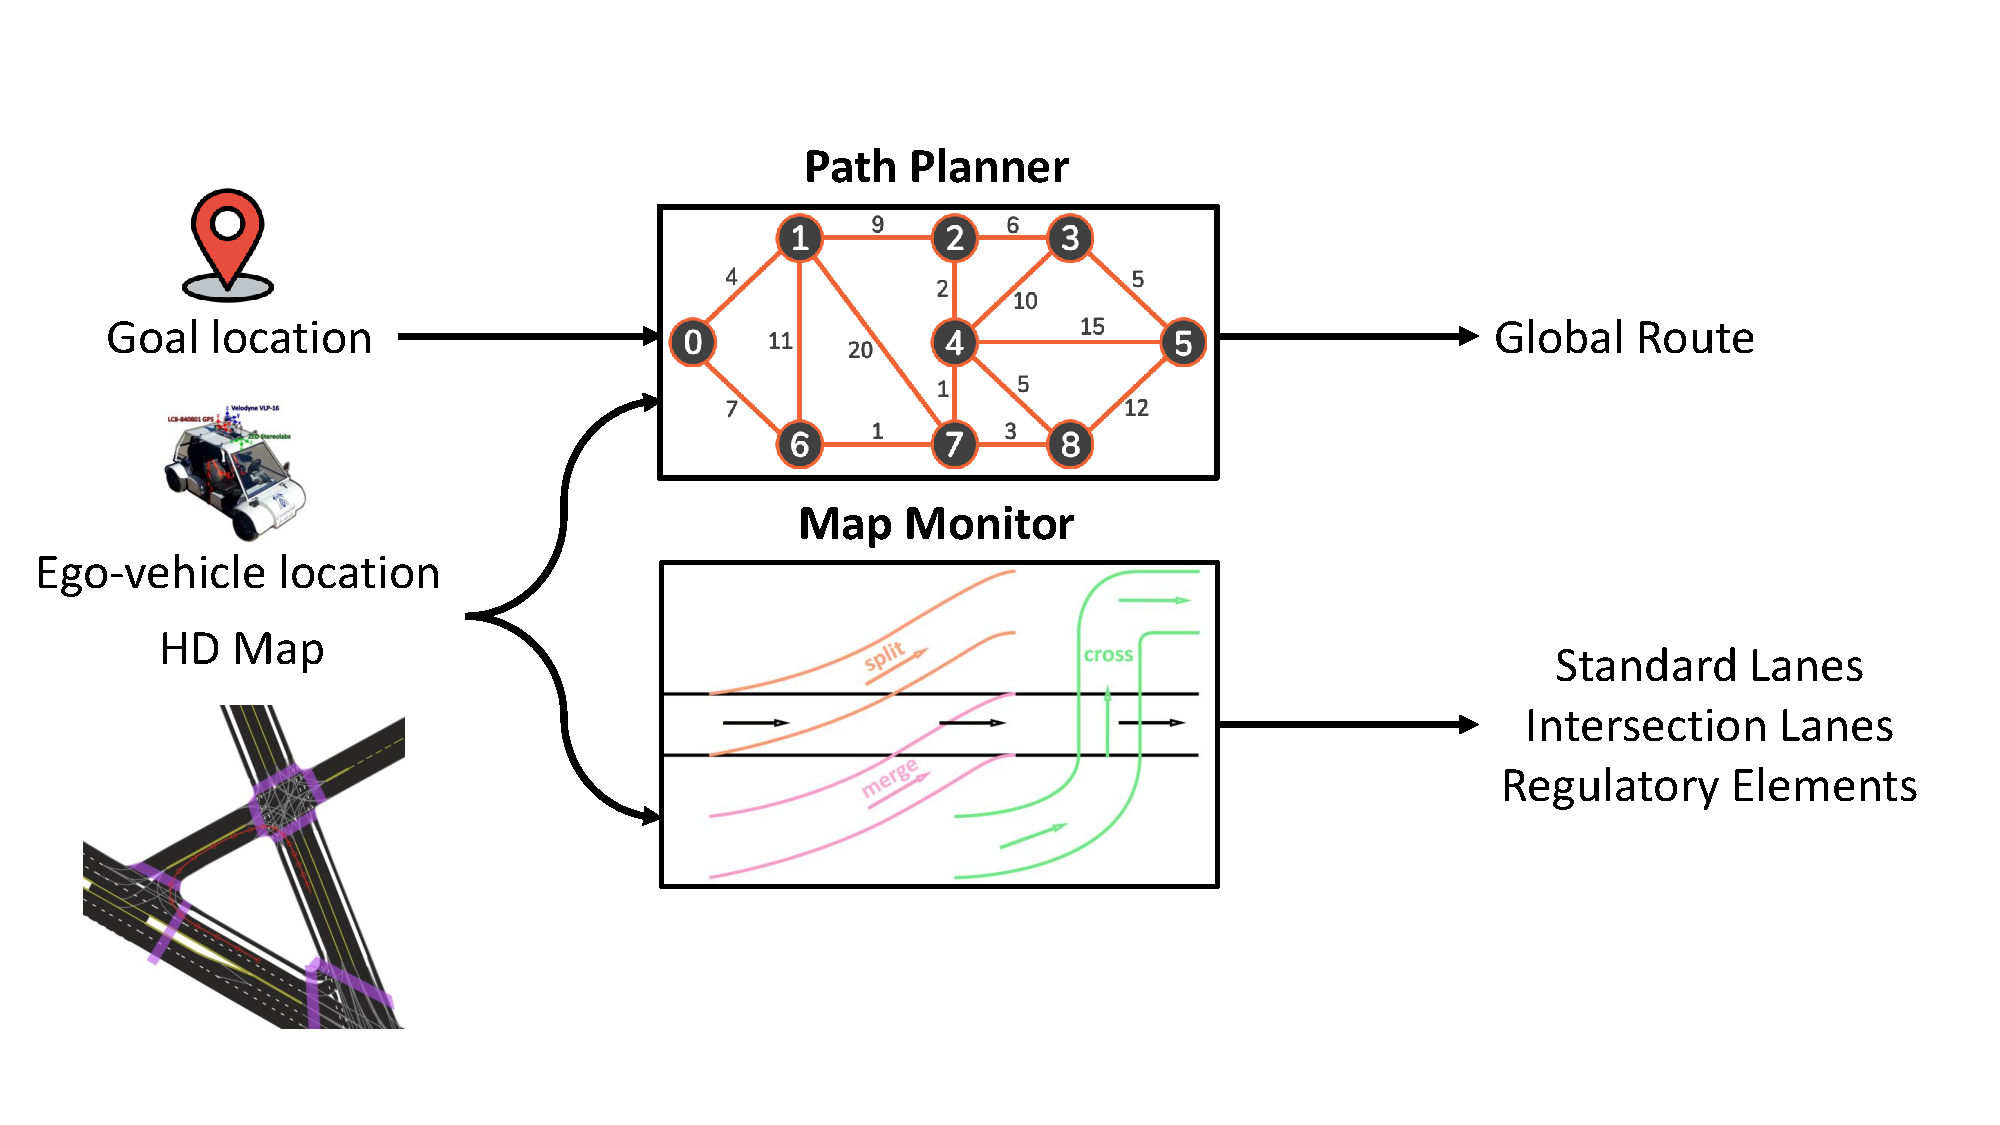
\includegraphics[width=0.8\textwidth]{chapter_4_SmartMOT/path_planner_map_monitor.pdf}
	\caption{Main uses of HD map: Path Planning and Map Monitoring}
	\label{fig:chapter_4_SmartMOT/path_planner_map_monitor}
\end{figure}

In particular, given a pre-defined global route, in this thesis we focus our interest on designing a map monitor module, responsible for retrieving the most relevant lanes around the ego-vehicle to enhance real-time perception and scene understanding requirements.

\subsubsection{Map Monitor}
\label{subsubsec:4_smartmot_mapmonitor}

In a similar way to humans that pay more attention to close obstacles, people walking towards them or upcoming turns rather than considering the presence of building or people far away, the perception layer of a self-driving car must be modelled to focus more on the salient regions of the scene \cite{sadeghian2019sophie} and the more relevant agents to predict the future behaviour of each traffic participant. In that sense, \acp{HDmap} have been widely adopted to provide offline (also known as context) information to complement the online information provided by the sensor suite of the vehicle and its corresponding algorithms. 

Recent learning-based approaches \cite{hong2019rules} \cite{chai2019multipath} \cite{gao2020vectornet} \cite{casas2018intentnet}, which present the benefit of having probabilistic interpretations of different behaviour hypotheses, require to build a representation to encode the trajectory and map information. \cite{hong2019rules} assumes that detections around the vehicle are provided and focuses its work on behaviour prediction by encoding entity interactions with ConvNets. Intentnet \cite{casas2018intentnet} proposes to jointly detect traffic participants (mostly focused on vehicles) and predict their trajectories using raw LiDAR pointcloud and rendered \ac{HDmap} information. PRECOG \cite{rhinehart2019precog} aims to capture the future stochasiticity by flow-based generative models. Furthermore, MultiPath \cite{chai2019multipath} uses ConvNets as encoder and adopts pre-defined trajectory anchors to regress multiple possible future trajectories. 

As observed, recent \ac{DL}-based techniques use relatively complicated filters to predict, in an accurate way, the spatial features of the obstacles in the scene, increasing the complexity and computational cost of the system. On the other hand, traditional methods for behaviour prediction are rule-based, where multiple behaviour hypothesis are generated based on constraints from the road maps. As stated above, road maps present some clear advantages over other perception sensors. Then, \acp{HDmap} can be an additional sensor that cannot fail unless the road infrastructure changes, providing meaningful, accurate and useful information in real-time operation.  

Regarding this, we design a Map Monitor in charge of monitoring the surrounding area of the vehicle. The inputs of the Map Monitor are the information provided by the Map Parser module (in charge of getting the information of the map from the \ac{HDmap} file and transform it into custom classes that can be used by other modules like Planning or Perception) and the waypoint route previously obtained by the path planner. The main goal of the Map Monitor is to only monitor the most relevant map elements around the ego-vehicle given the route provided by the global planner (or a new route if the local planer decides to recalculate the route). This Map Monitor was published (where I am a co-author) in the following conference paper \cite{diaz2022hd}: "HD maps: Exploiting OpenDRIVE potential for Path Planning and Map Monitoring", 2022 IEEE Intelligent Vehicles Symposium (IV), p. 1211-1217. 

First, the path planner returns the route that is divided in segments separated by a given distance and calculates in which segment of the route the ego-vehicle is found, activating a flag in such a way the Map Monitor can start operating. Otherwise, in case the ego-vehicle cannot be located inside the route, the Map Monitor is deactivated. Secondly, a monitor callback is called periodically every time the ego-vehicle status (position, velocity, orientation, etc.) is received, as observed in Figure \ref{fig:chapter_4_SmartMOT/IV_2021}. This callback evaluates, if the Map Monitor module is active, calculates the monitored elements frontwards and backwards for a given distance which is proportional to the ego-vehicle velocity given a braking distance linear model that establishes a linear regression between two arrays of velocity and braking distance data. Nevertheless, we make use of a threshold distance to still monitor the environment if the ego-vehicle is stopped. %We will detail the corresponding hyperparameters in Chapter \ref{sec:4_mot_and_euroncap}.

The monitored elements are:

\begin{itemize}
	
	\item \textbf{Standard Lanes}: Current, back and the corresponding left and right lanes. Current lane is monitored from current position to a dynamic distance depending on the velocity of the ego-vehicle. Back lane is monitored from current position to back a proportional distance of the dynamic current lane obtained distance. Left and right lanes are monitored the same distance that current and back only if the lane marking from the \ac{HDmap} data allows the lane change.
	
	\item \textbf{Intersection Lanes}: Other lanes that intersect the current monitored lane are checked. Intersection lanes can have different roles: split (1 lane splits into 2 or more), merge (2 or more lanes merge into 1) and cross (a lane crosses a part of the current lane). To calculate the intersection lanes, each lane of every junction (junctions are areas where more than 2 roads meet) in the current lane is evaluated. The polygon of each lane is calculated and evaluated if is inside the polygon of the current lane. It is important to consider that roundabouts are considered as a set of multiple junctions. 
	
	\item \textbf{Regulatory Elements}: The monitored elements are stops, giveaways, traffic lights, speed limits and crosswalks. The regulatory elements are only monitored for the next intersection affecting the route. 
	
\end{itemize}

An example of our map monitor module in the CARLA simulator \cite{dosovitskiy2017carla} using the \ac{RVIZ} \cite{quigley2009ros} may be observed in Figure \ref{fig:chapter_4_SmartMOT/monitored_area_CARLA_ROS}.

\begin{figure}[h] 
	\centering
	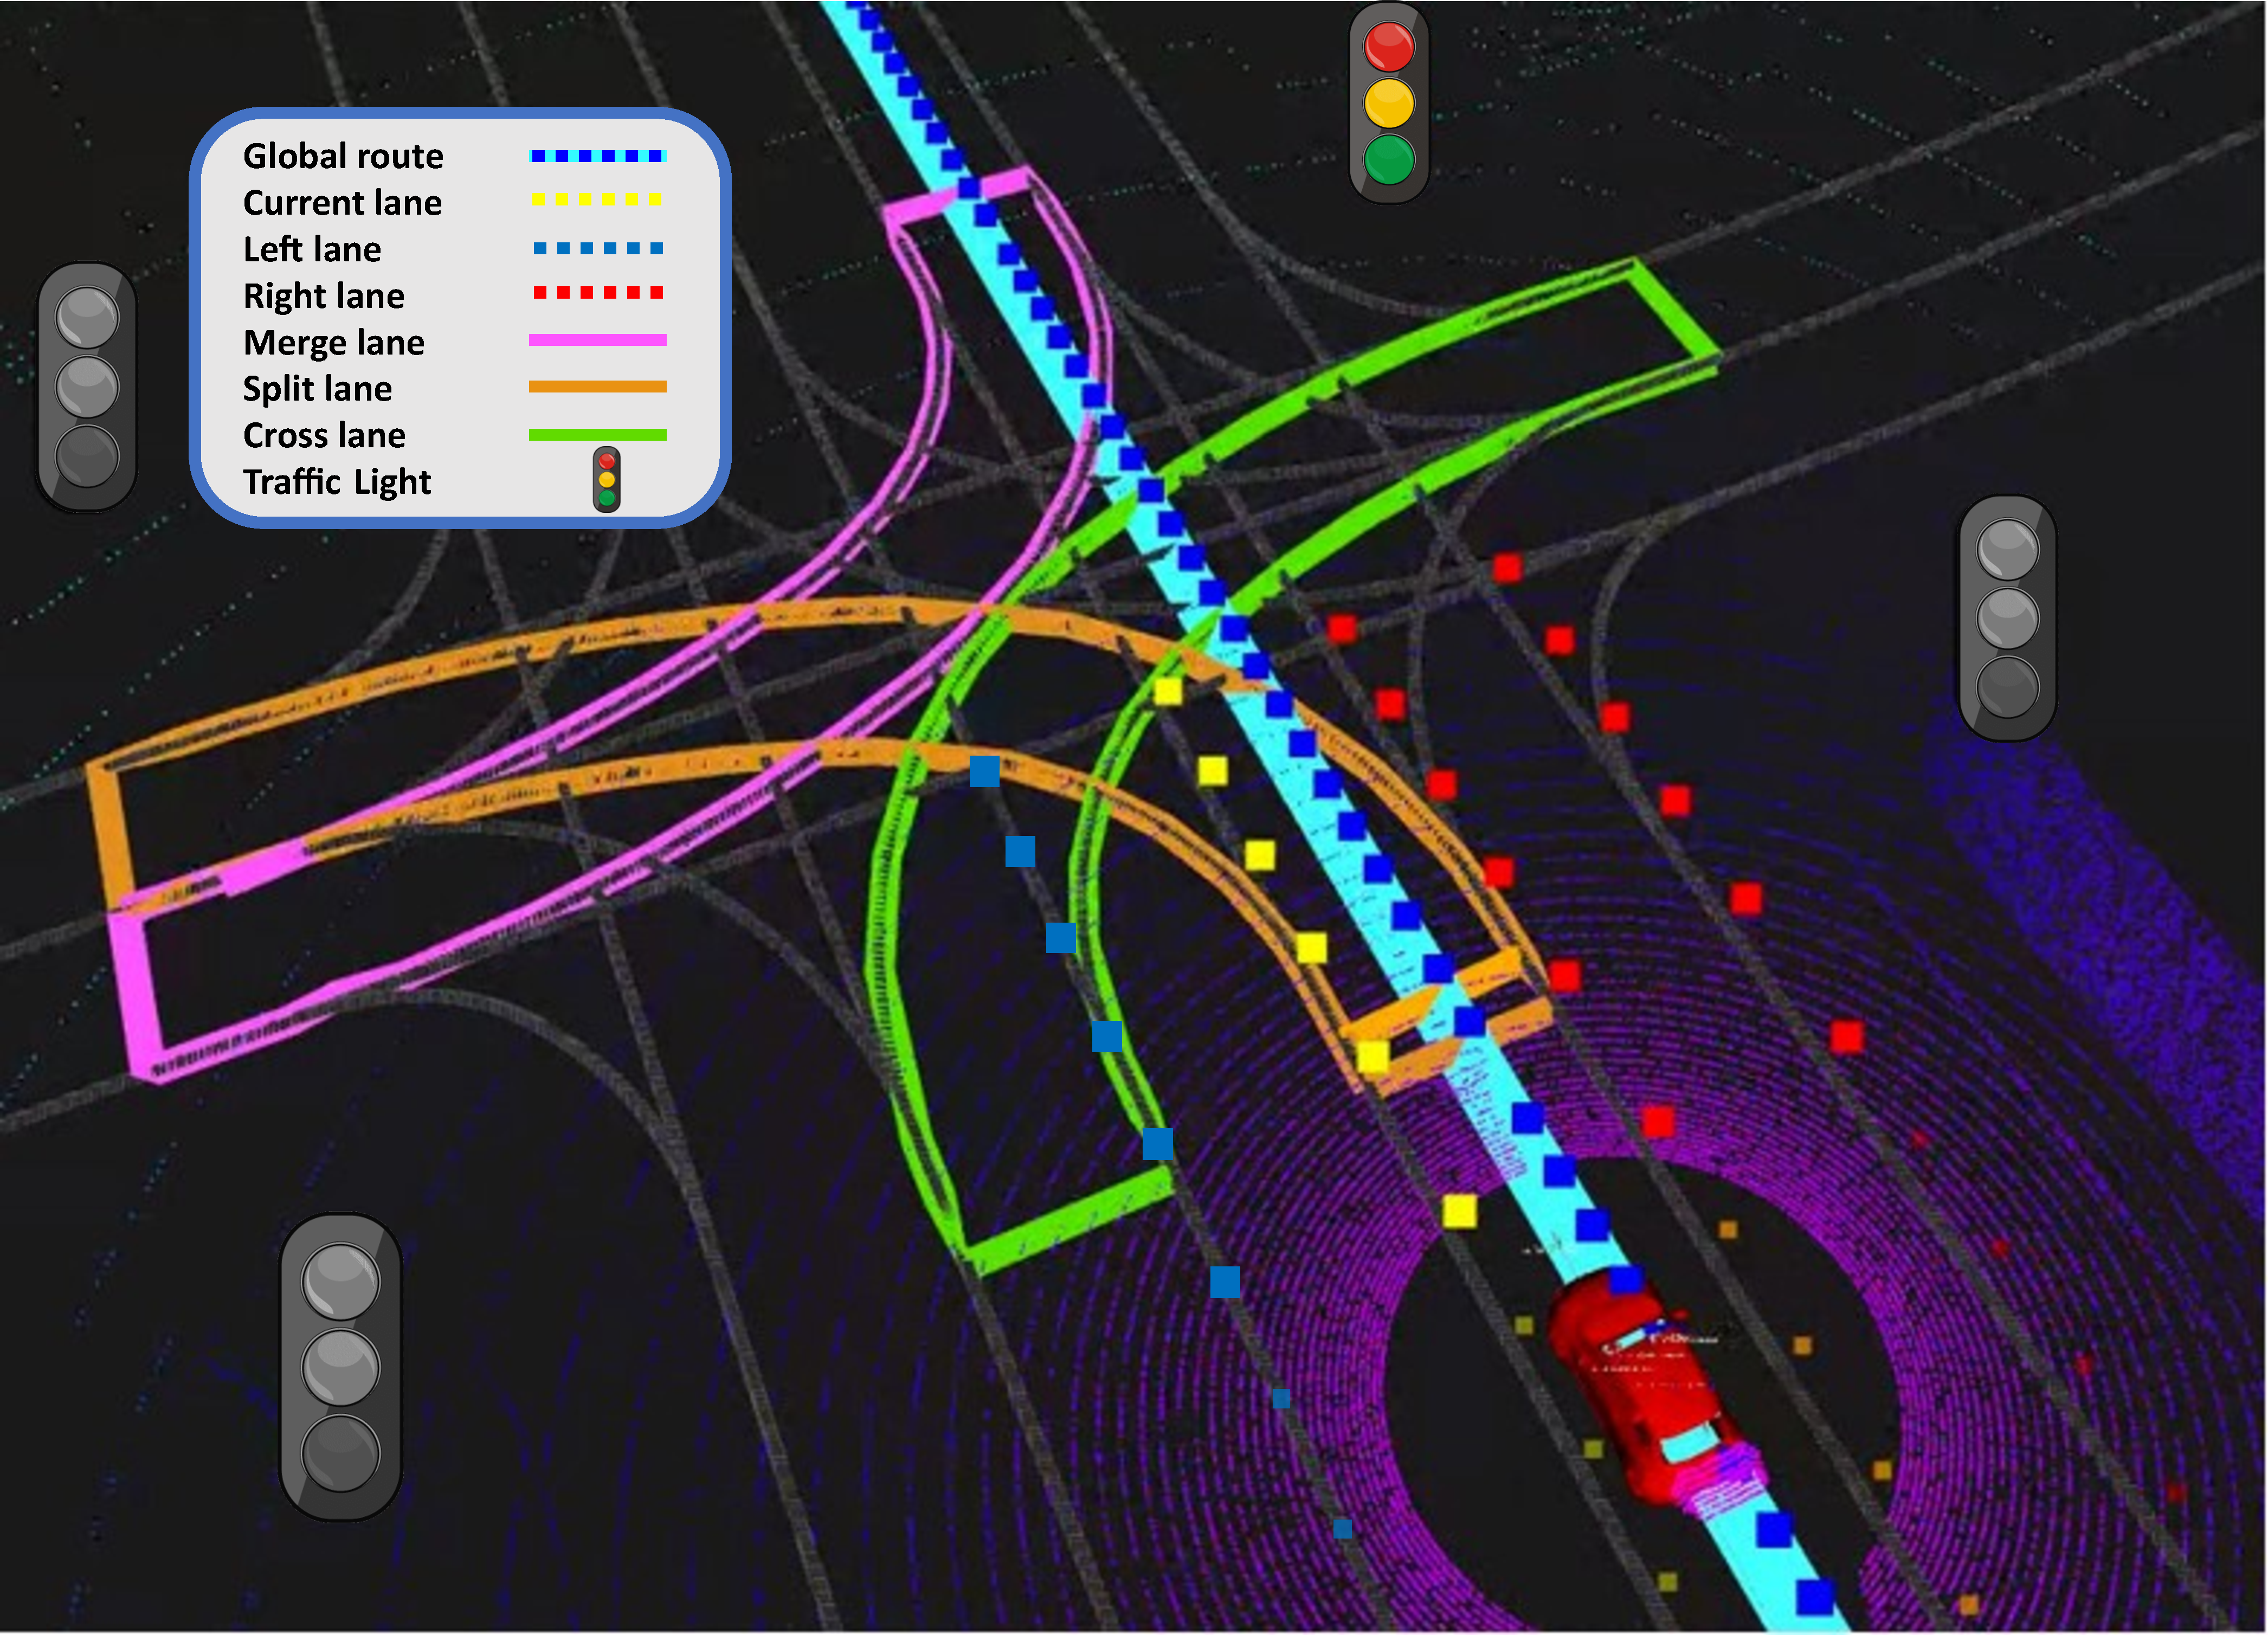
\includegraphics[width=0.6\textwidth]{chapter_4_SmartMOT/lane_types.pdf}
	\captionsetup{justification=justified}
	\caption[Monitored area in the CARLA simulator using the RVIZ tool]{Monitored area in the CARLA simulator using the RVIZ tool. It can be appreciated the visualization of the global route, standard lanes, intersection lanes and different traffic lights (regulatory elements). Note that the relevant traffic light is coloured while remaining ones are masked.}
	\label{fig:chapter_4_SmartMOT/monitored_area_CARLA_ROS}
\end{figure}

As illustrated in Figure \ref{fig:chapter_4_SmartMOT/IV_2021}, once the object detections have been provided and the monitored area has been computed, the Monitored Lanes-based Attention Module helps us to increase the efficiency and robustness of the system to avoid tracking and predicting all obstacles in the environment, which would escalate the computational cost especially in arbitrarily complex urban scenario. 

\begin{figure}[h] 
	\centering
	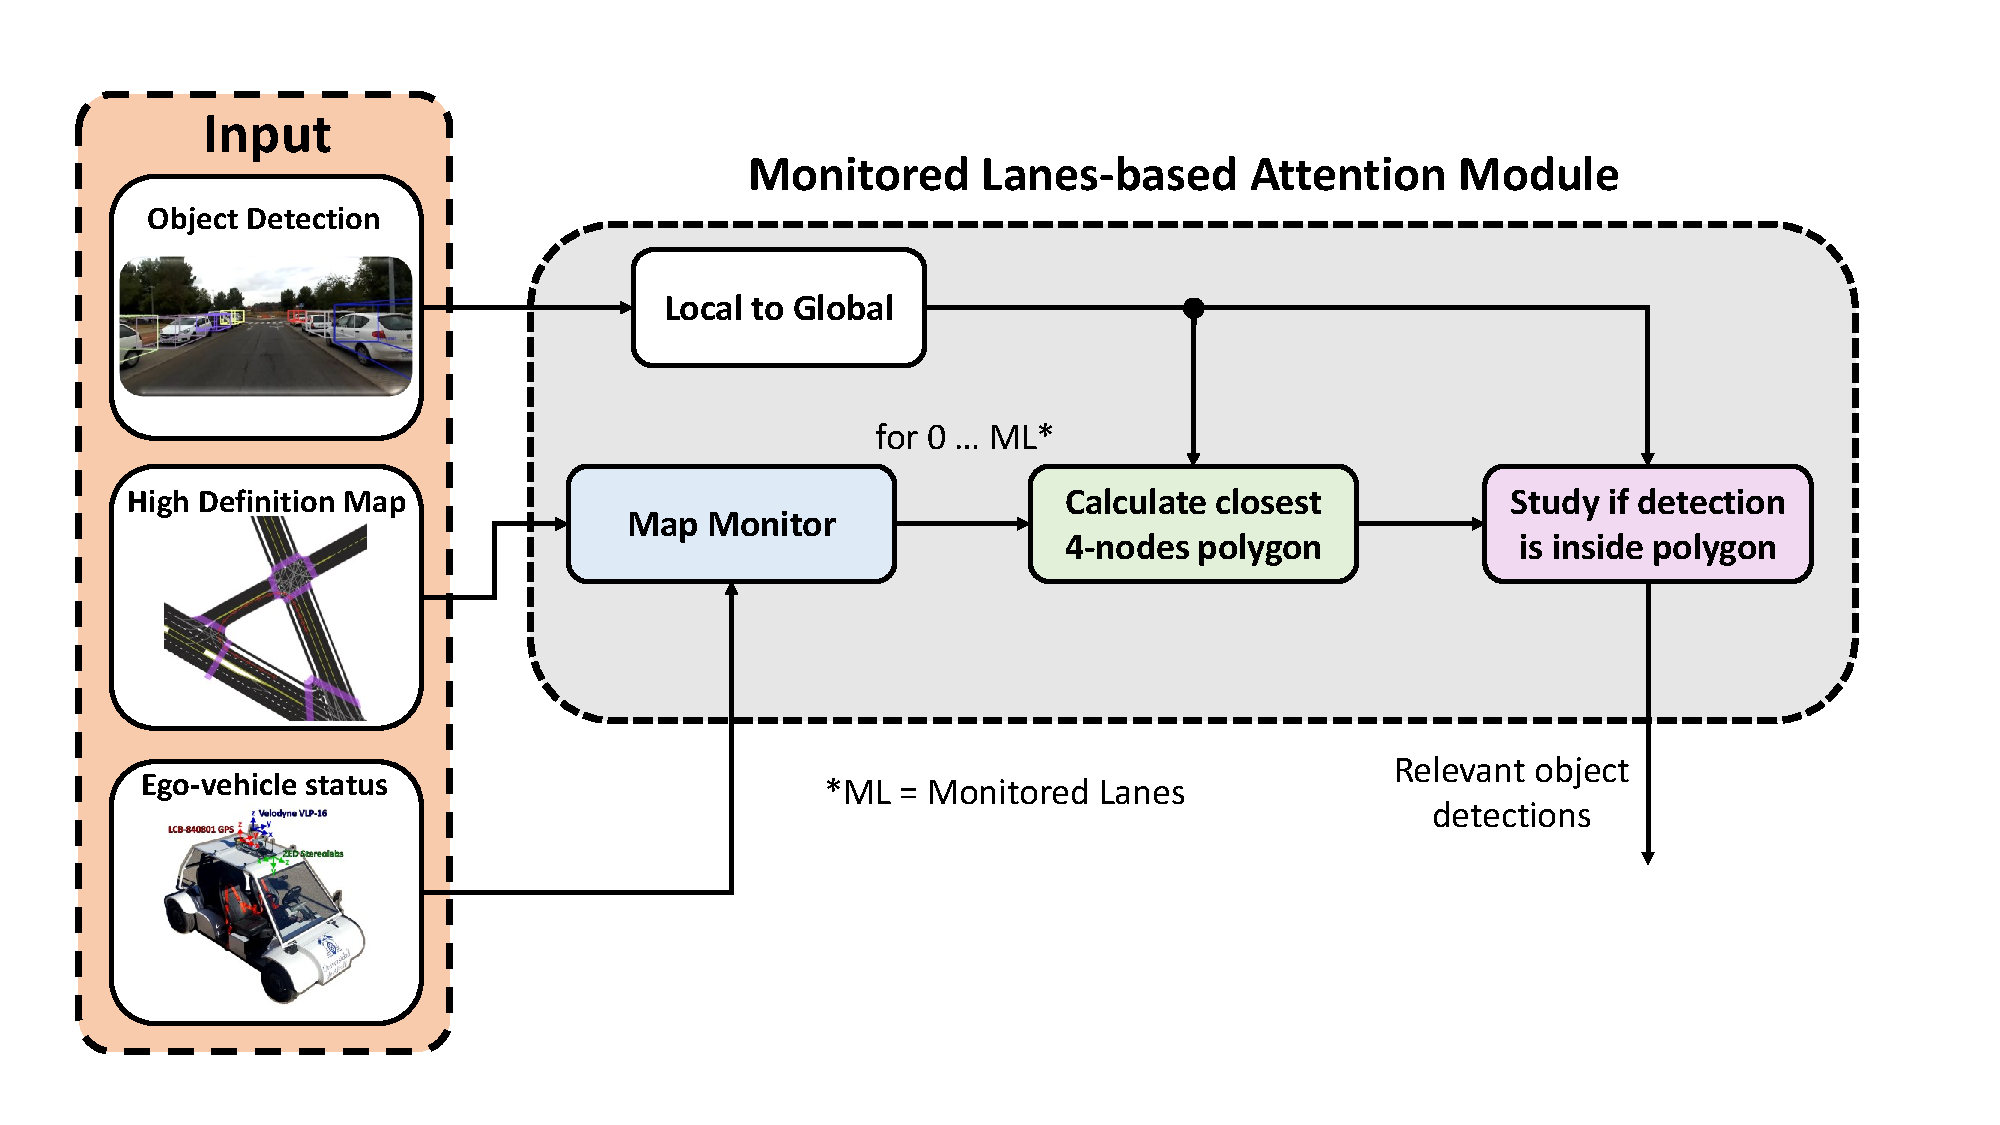
\includegraphics[trim=0 1cm 3cm 1cm, width=0.8\textwidth]{chapter_4_SmartMOT/monitored_lanes_based_attention_module.pdf}
	\captionsetup{justification=justified}
	\caption[Overview of our proposed Monitored Lanes-based Attention module to filter non-relevant object detections]{Overview of our proposed Monitored Lanes-based Attention module to filter non-relevant object detections. Note that in order to study if a detection is inside a polygon, we make use of the Jordan's Curve Theorem. Moreover, if the object detection is a \ac{VRU}, the closest polygon is widened towards the sidewalk. Both map, ego-vehicle status and object detection must be in global (map) coordinates.}
	\label{fig:chapter_4_SmartMOT/monitored_lanes_based_attention_module}
\end{figure}

This attention module is not focused on \ac{DL} because the main purpose is to filter non-relevant obstacles in an efficient and interpretable way, such as agents driving way in opposite direction lanes, parked vehicles or pedestrians who are chatting on the sidewalk. The filtering process carried out by our Monitored Lanes-based Attention Module is illustrated in Figure \ref{fig:chapter_4_SmartMOT/monitored_lanes_based_attention_module} and summarized as follows:

\begin{algorithm}[h]
	\SetAlgoLined
	\KwData{point, polygon}
	\KwResult{isInside}
	crossings $\leftarrow$ 0\;
	\For{i from 0 to (polygon.length - 1)}{
		vertex1 $\leftarrow$ polygon[i]\;
		vertex2 $\leftarrow$ polygon[(i + 1) mod polygon.length]\;
		\If{(point.y > min(vertex1.y, vertex2.y)) \textbf{and} (point.y $\leq$ max(vertex1.y, vertex2.y))}{
			\If{point.x $\leq$ max(vertex1.x, vertex2.x)}{
				\If{vertex1.y $\neq$ vertex2.y}{
					xIntersection $\leftarrow$ (point.y - vertex1.y) * (vertex2.x - vertex1.x) / (vertex2.y - vertex1.y) + vertex1.x\;
					\If{vertex1.x == vertex2.x \textbf{or} point.x $\leq$ xIntersection}{
						crossings $\leftarrow$ crossings + 1\;
					}
				}
			}
		}
	}
	isInside $\leftarrow$ (crossings \% 2 == 1)\;
	\KwRet{isInside}\;
	\caption{Jordan's Curve theorem to determine if a point is inside a polygon}
	\label{alg:4_jordan_curve_theorem}
\end{algorithm}

\begin{enumerate}
	
	\item We determine the lanes of interest around the vehicle provided by the map monitor, until a given threshold, which will depend on the ego-vehicle velocity. The minimum information will be the current front and back lane information (mandatory for the \ac{ACC} and Unexpected \ac{VRU} use cases), as well as left and right lane information, if lane change is available considering the presence of a discontinuous line. Moreover, if an intersection is near the ego-vehicle, other lanes of interest such as merging, splits and intersections are considered (see Figure \ref{fig:chapter_4_SmartMOT/monitored_area_CARLA_ROS}), which are specially useful in urban scenarios.% when the vehicle faces a roundabout or other vehicles incorporation in an intersection.
	
	\item In order to consider an agent as relevant, we study the presence of this agent in our monitored lanes. The main idea is to find the closest polygon segment (two nodes on the left, same on the right) to the agent. To do that, we iteratively compute the $\mathcal{L}_2$ distance between the agent position (transformed into global (\aka \ map) coordinates) and the left way nodes (starting from the beginning) of a certain lane. Note that it is irrelevant to take either the left or right way in terms of observing if the detection is inside a polygon made up by four nodes of the lane, such as there exists the same number of nodes for both ways. For example, in the case of an agent located in front of the vehicle, the distance will decrease since the subsequent left way nodes are closer to the agent. 
	
	\item Once the new calculated distance is greater than the previous value, that means the closest segment with nodes \textit{$N_0$} and \textit{$N_1$} are found. Taking the same lane indexes in the right way, we obtain a four-side polygon in which the detection is evaluated using the Jordan's curve theorem \cite{tverberg1980proof}, as depicted in Algorithm \ref{alg:4_jordan_curve_theorem}. In this theorem, the input parameters are a point and a polygon, where, by means of a simple-yet-accurate ray casting algorithm, a loop is used to iterate over the polygon vertices and performs the necessary checks to determine the number of crossings. The Jordan's Curve Theorem states that a point is inside a polygon if the number of crossings from an arbitrary direction is odd. Consequently, in our particular case, if the object detection lies outside the closest polygon segment, the traffic participant is considered as non-relevant.
	
	\item Nevertheless, despite this proposal is coherent for non-holonomic obstacles with more constrained behaviours like cars, vans or trucks, the behaviour of \acfp{VRU}, is usually difficult to predict. Hence, we widen the closest segment area a certain threshold \textit{L} to the sidewalk so as to track the closest \acp{VRU} to the road. Note that according to the \ac{ITS} society, \acp{VRU} are road users not in a car, bus or truck, generally considered to include pedestrians, motorcycle riders, cyclists, children 7-years and under, the elderly and users of mobility devices.
	
\end{enumerate}

\subsection{BEV Kalman Filter: State Prediction}
\label{subsec:4_smartmot_state_prediction}

Once we have obtained the most relevant \ac{BEV} detections of the environment, a \ac{BEV} \ac{KF} is used to track the objects. To predict the state of object trajectories from the previous frames to the current frame, we approximate objects inter-frame displacement using a constant velocity model, which is independent of other objects in the scene and of the \ac{LiDAR} motion. Regarding this, the estimation of the measured variables in the following frame are:

\begin{equation}
	\begin{split}
		x_{px}(\hat{t})=x_{px}(t)+v_{x} \\
		y_{px}(\hat{t})=y_{px}(t)+v_{y} \\
		s(\hat{t})=s(t)+v_{s} \\
		\theta(\hat{t})=\theta(t)+v_{\theta}
	\end{split}
\end{equation}

Since we formulate the tracking problem over the \ac{BEV} plane, we remove all variables related to the $\textit{z}$-coordinate of the object. On the other hand, since our tracking-by-detection algorithm is inspired by the well-established \ac{SORT} \cite{bewley2016simple} tracking algorithm, originally proposed to track pedestrians using videos as input, some additional variables are included in the object state, such as the aspect ratio and the scale of the bounding box, to help in the tracking stage. The aspect ratio can be defined as the relation between the width and the length of the obstacle. Likewise, the scale represents the area of the target bounding box. Then, the state of each object tracker (usually referred as trajectory tracker in the literature) can be expressed as:

\begin{equation}
	\label{state}
	T_{t}^{j} = [x_{px},y_{px},s,r,\theta,x_{px}^{'},y_{px}^{'},s^{'},\theta^{'}]
\end{equation}

Note that the angular velocity $\theta^{'}$ is used in the state space to improve the prediction of the obstacle in later frames. Furthermore, as shown in \cite{bewley2016simple}, the aspect ratio of the bounding box is considered to be constant. As observed in Figure \ref{fig:chapter_4_SmartMOT/IV_2021}, at every frame \textit{t}, a tuple $T_{t}=[T_{t}^{1},T_{t}^{2}, ...,T_{t}^{M}]$ is returned by the data association module, where each element correspond to an association between a detection and a tracker. Note that $M$ represents the current number of trackers. Then, based on these associations between trackers of the previous frame and current detections, and assuming a 1st-order \ac{KF} (constant velocity model), the tuple $T_{\hat{t}}$ is calculated, where each element corresponds to the predicted trajectory ($T_{\hat{t}}^{j}$) in the current frame $\textit{t}$ expressed as:

\begin{equation}
	\label{est}
	T_{\hat{t}}^{j} = [x_{px}(\hat{t}),y_{px}(\hat{t}),s(\hat{t}),r,\theta(\hat{t}),x_{px}^{'},y_{px}^{'},s^{'},\theta^{'}]
\end{equation}

This tuple of predicted trajectories based on the previous frame associations, in addition to the current frame detections, represents the inputs to the data association algorithm at frame $t$.

\subsection{Data association}
\label{subsec:4_smartmot_data_association}

In order to associate the detections $D_{t}$ and the trackers information after the \ac{KF} state prediction $T_{\hat{t}}$, the \acf{HA} is applied. The resulting affinity matrix presents $N$ rows (number of filtered detections after the monitored lanes-based attention module at frame $t$) and $M$ columns, which correspond to the number of predicted trajectories (\ie \ the trackers) based on the information of frame $t-1$. Each element of the matrix corresponds to the \ac{IOU} in the \ac{BEV} plane between every pair of predicted trajectory and detection. 

Then, following the principles stated in the \ac{HA} stated in Chapter \ref{subsec:3_HA_formulation}, we solve the bipartite graph matching problem, rejecting the matching if the \ac{BEV}-\ac{IOU} metric is lower than a given hyperparameter $IoU_{th}$, giving rise to a set of matched detections ($D_{matched}$) and predicted trackers ($T_{matched}$) with the same length $H$ (the number of matches), as well as a set of unmatched detections ($D_{unmatched}$), where $P = N - H$ is the number of unmatched detections, and a set of unmatched trajectories ($T_{unmatched}$), where $Q = M - H$ is the number of unmatched trackers.

\subsection{BEV Kalman Filter - Object State Update}
\label{subsec:4_smartmot_data_state_update}

As observed in Figure \ref{fig:chapter_4_SmartMOT/IV_2021}, once we have the corresponding sets of matched detections and trajectories, based on the \ac{KF} prediction-update cycle, we update the state space of each trajectory based on its corresponding matched detection. To do that, we use the weighted average between the matched detection values and the state space of the trajectory tracker, according to \cite{kalman1960new}. 

On the other hand, in the same way that \cite{weng20203d}, we appreciate that this state update does not work properly for obstacle orientation. The reason is simple: Unless the object detector is based on sensor fusion and vision information is included, the object detector cannot distinguish if the obstacle is rotated 0 or $\pi$, $\frac{\pi}{2}$ and $\frac{3\pi}{2}$, and so on, around its \textit{z}-axis. That is, the orientation may differ by $\pi$ in two consecutive frames. Then, if no orientation correction is applied, the \ac{KF} associated to the tracker can get easily confused, since it tries to adapts itself to the new orientation value rotating the object by $\pi$ in following frames, giving rise to a low \ac{BEV}-\ac{IOU} between new detections and predicted trajectories. 

In that sense, regarding the assumption that obstacles must move smoothly and its orientation cannot be modified by $\pi$ in one frame (0.1 s assuming a frequency of 10 Hz), when this happens the orientation of the corresponding matched detection or matched tracker can be considered wrong. To solve this problem, the detection module only considers angle from 0 to $\pi$ (that is, if an angle exceeds $\pi$, it is substracted to the provided angle). Moreover, if the difference of orientation between a given matched detection and its corresponding matched trajectory is greater than $\frac{\pi}{2}$, as stated before, either the orientation of the detection or the orientation of the tracker is wrong. Finally, we add $\pi$ to the orientation of the tracker with the aim to be consistent with the matched detection. 

\subsection{Deletion and Creation of Track Identities}
\label{subsec:4_smartmot_data_deletion_creation}

When obstacles leave and enter the aforementioned monitored lanes, unique identities must be destroyed or created accordingly. In most tracking algorithms it is known as the Birth and Death Memory, which is based on the set of unmatched trackers and detections provided by the data association algorithm, where the unmatched trackers represent potential objects leaving the monitored area, in the same way that unmatched detections represent potential objects entering in the area of interest. 

In order to avoid tracking of false positives or non-relevant obstacles, a new tracker is not created until the unmatched detection has been continuously detected in the next $f_{min}$ frames. Then, the tracker is initialized with the features of the detected bounding box, and the associated velocities set to zero. Note that, as stated in \cite{bewley2016simple}, since the velocity associated to the measured variables is unobserved at this moment (\ie \, tracker initialization), the covariance initializes the value of the velocities (in the present work, velocity of the $x_{px},y_{px}$ centroid, scale $s$ and rotation angle $\theta$) with large values, reflecting their uncertainty. 

To avoid removing true positives trajectories from the scene, they are not terminated unless they are not detected during consecutive $a_{max}$ frames. This assumption prevents an unbounded growth in the number of localization errors and trackers due to predictions over long duration where the object detector does not provide any correction. Note that since this work does not consider object re-identification for simplicity, an object should leaves the scene and then reappears, according to the \ac{SORT} algorithm, if it is initialized with a new tracker under a new identity. As shown in Figure \ref{fig:chapter_4_SmartMOT/IV_2021}, the inputs to the Matched Trackers module are the updated matched trajectories from the \ac{BEV} \ac{KF} and a set of created and deleted trackers, which jointly represent the input trajectories for the prediction step in the following frame.

\subsection{\ac{CTRV} uni-modal prediction}
\label{subsec:4_smartmot_ctrv_prediction}

The last stage of our SmartMOT pipeline is a physics-based \ac{MP} model to predict the future behaviour of the agents in the short-term. In particular, we make use of the previously studied \ac{CTRV} model. Once the tracker information (position, velocity and orientation) has been retrieved in real-world coordinates (instead of \ac{BEV} image coordinates), we are able to differentiate between static and dynamic agents. Then, given the ego-vehicle status and dynamic agents short-term prediction, we analyze the risk of collision or carry out the state of the current behaviour (\ac{ACC}, Pedestrian Crossing, Give way, and so forth and so on) in such a way SmartMOT can send the corresponding signal to the \ac{DM} layer. %Figure \ref{fig:chapter_4_SmartMOT/filtering_process_example} illustrates an example of the filtering process, tracking-by-detection paradigm and \ac{CTRV} prediction.
\begin{comment}
\begin{figure}[] 
	\centering
	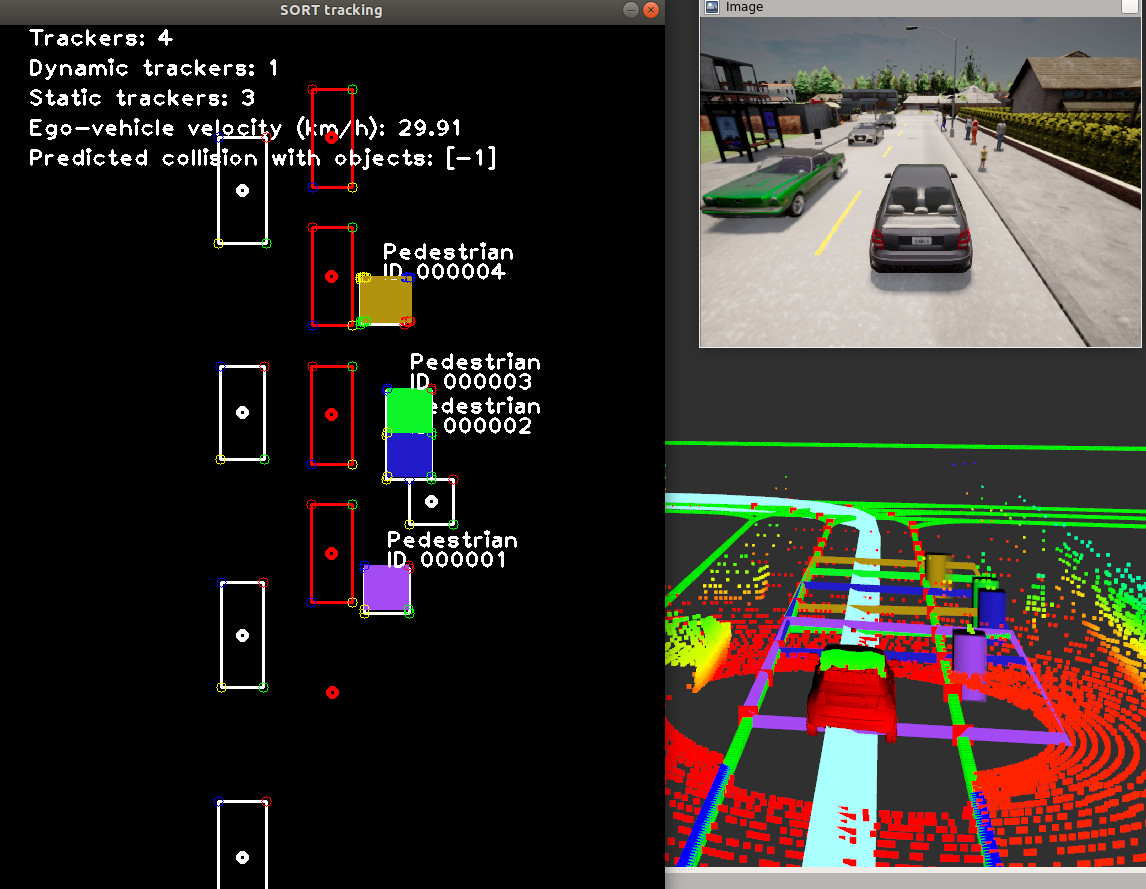
\includegraphics[width=0.8\textwidth]{chapter_4_SmartMOT/filtering_process_example.jpg}
	\captionsetup{justification=justified}
	\caption[Simulation use case of SmartMOT in the \ac{CARLA} simulator]{Simulation use case of SmartMOT in the \ac{CARLA} simulator: Non-relevant objects are filtered by means of the monitored lanes-based attention module. Nevertheless, \acfp{VRU} are considered on the sidewalk if they are close enough to the closest segment of the corresponding monitored lane.}
	\label{fig:chapter_4_SmartMOT/filtering_process_example}
\end{figure} 
\end{comment}

\section{Experimental results}
\label{sec:4_mot}

We validate our proposed tracking algorithm (SmartMOT) using the KITTI \ac{MOT} benchmark \cite{geiger2012we} in a quantitative and qualitative way, as well as using some \ac{LiDAR} recorded data from our campus to observe some qualitative results and a comparison of inference frequency using an edge-computing device and standard Personal Computer (PC) desktop. Finally, we study some interesting scenarios in the \ac{CARLA} simulator where map information is included in order to appreciate how the inference time of the \ac{MOT} may be drastically reduced when the system pays attention to the most relevant agents around the \ac{ADS} according to the current traffic scenario. 

% Then, we conduct an interesting study of how integrating the monitored area can reduce the risk of collision and/or the impact velocity on the \ac{VRU}.

\subsection{Dataset}
\label{subsec:4_mot_dataset}

In order to evaluate our proposed \ac{MOT} system pipeline, we carry out the evaluation in the KITTI \ac{MOT} benchmark \cite{geiger2012we} based on the method proposed by \cite{weng20203d}. This is composed of 29 testing and 21 training/validation video sequences, where each sequence is provided with RGB images (left and right camera of the stereo pair), \ac{LiDAR} point-cloud and the corresponding calibration file. Since KITTI does not provide any annotation (\ie, the ground-truth) for the testing split, we decided to evaluate our system in the training/validation split. Moreover, although KITTI distinguish among eight different classes for the object type, our work focus on the car subset, since it is the class that contains the most number of instances over the whole benchmark.

\subsection{Multi-Object Tracking metrics}
\label{subsec:4_mot_metrics}

Mainstream metrics applied to MOT systems are extracted from CLEAR \ac{MOT} metrics \cite{bernardin2008evaluating}, such as \acf{MOTA} and \acf{MOTP}. These metrics provide a comprehensive assessment of tracking performance by considering aspects such as accuracy, precision, and overall performance. Now, the main metrics are described:

\subsubsection{Multi-Object Tracking Accuracy (MOTA)}
\label{subsubsec:4_MOTA}

The \acf{MOTA} metric is commonly used to evaluate the performance of multi-object tracking algorithms. It measures the overall tracking accuracy by considering the \acp{FP}, \acp{FN}, and \ac{IDS} in the tracking results. The formula for calculating \ac{MOTA} is given as:

\begin{equation}
	MOTA = 1 - \frac{{\text{{FN}} + \text{{FP}} + \text{{IDS}}}}{{\text{{GT}}}}
\end{equation}

where:

\begin{itemize}
	
	\item \textbf{FN (False Negatives)} represents the number of ground-truth objects that were not correctly detected by the tracking algorithm.
	
	\item \textbf{FP (False Positives)} represents the number of false detections made by the tracking algorithm.
	
	\item \textbf{IDS (Identity Switches)} represents the number of times the algorithm incorrectly switches the identity of a tracked object.
	
	\item \textbf{GT (Ground-Truth)} represents the total number of ground-truth objects in the video sequence.
	
\end{itemize}

A higher \ac{MOTA} value indicates better tracking accuracy, with a perfect tracking result yielding MOTA = 1.

\subsubsection{Multi-Object Tracking Precision (MOTP)}
\label{subsubsec:4_MOTP}

The \acf{MOTP} metric is used to assess the localization accuracy of a \ac{MOT} algorithm. It measures the average precision of the tracked object positions by considering the distance between the predicted locations and their corresponding ground truth locations. The formula for calculating \ac{MOTP} is given as:

\begin{equation}
	MOTP = \frac{{\sum_{{i=1}}^{{N}} d_i}}{{N}}
\end{equation}

where:

\begin{itemize}
	
	\item \textbf{\(N\)} represents the total number of matched object pairs between the predicted and ground truth locations.
	
	\item \textbf{\(d_i\)} represents the $\mathcal{L}_2$ between the predicted location and the ground-truth location for the \(i\)-th matched object pair.
	
\end{itemize}

The \ac{MOTP} metric ranges between 0 and 1, with a higher value indicating better localization accuracy. A perfect tracking result with exact object positions would yield \ac{MOTP} = 1.

\subsubsection{Integral metrics: AMOTA and AMOTP}
\label{subsubsec:4_integral_metrics}

Previous \ac{MOT} metrics analyze the \ac{MOT} system performance at a given threshold, not taking into account the confidence provided by the object detector and possibly misunderstanding the capability of the method. That means they do not take into account the full spectrum of precision and accuracy over different thresholds. Moreover, as discussed by AB3DMOT \cite{weng20203d}, KITTI 2DMOT evaluates the performance \ac{MOT} by means of aforementioned traditional CLEAR \ac{MOT} metrics, where the detected 3D bounding box onto the image plane. As expected, this does not demonstrate the full strength of 3D \ac{DAMOT}. 

In that sense, AB3DMOT \cite{weng2019baseline} recently presented a 3D extension of the KITTI 2DMOT evaluation, known as KITTI-3DMOT, which introduces two new integral \ac{MOT} metrics to solve the problem of evaluating the \ac{MOTA} and \ac{MOTP} of the system across all detection thresholds, known as \ac{AMOTA} and \ac{AMOTP}, as shown in Equation \ref{eq:4_amota}:

\begin{equation}
	\label{eq:4_amota}
	AMOTA = \frac{1}{L}\sum_{\{\frac{1}{L},\frac{2}{L},...,1\}}(1-\frac{FP+FN+IDS}{num_{gt}})
\end{equation}

Where $L$ is the number of different recall values. Note that \ac{IDS}, \acp{FP} and \acp{FN} are modified according to the results of each threshold value. Likewise, \ac{AMOTP} can be estimated by integrating the \ac{MOTP} metric across all recall values. We will use these integral metrics, in addition to the aforementioned CLEAR \ac{MOT} metrics, to demonstrate the effectiveness of our tracking pipeline. Note that, since both \ac{AMOTA} and \ac{AMOTP} metrics are the integral of the corresponding metrics over different detection thresholds, as expected, the follow the same principle: the higher, the better. Note that in our proposed method (\ac{BEV} based), in order to compare our results with other \ac{SOTA} approaches in the 3D space using the aforementioned KITTI-3DMOT tool, we simply retrieve $z$-information (centroid, bounding box height) from the object detection stage.

\subsection{Comparison with the State-of-the-Art}
\label{subsec:4_mot_leaderboard}

We compare our proposed SmartMOT pipeline (PointPillars as 3D object detector \cite{lang2019pointpillars}, \ac{BEV} \ac{KF} as data estimator and \ac{HA} as data association algorithm excluding the map monitoring and filtering process in this case), against modern open-sourced 3D MOT systems such as mmMOT \cite{zhang2019robust}, FANTrack \cite{baser2019fantrack} and Monocular3D \cite{weng2019monocular} using the proposed KITTI-3DMOT. Results are observed in Table \ref{table:4_MOT_pipelines_validation}, where we achieve results that are up-to-pair with other \ac{SOTA} tracking methods. Note that these results were obtained with default values of the hyperparameters in the tracking stage ($age_{max}$ = 1, $min_{hits}$ = 1, $IoU_{thr}$ = 0.1). 

\begin{table}[h]
	\captionsetup{justification=justified}
	\caption[Comparative of Multi-Object Tracking pipelines using the KITTI-3DMOT evaluation tool in the validation set (car class)]{Comparative of Multi-Object Tracking pipelines using the KITTI-3DMOT evaluation tool in the validation set (car class). We bold the best results in \textbf{black} and the second best in \boldblue{blue} for each metric.}
	\label{table:4_MOT_pipelines_validation}
	\centering
	\resizebox{\linewidth}{!}{
		\begin{tabular}{c | ccccc}
			\toprule
			Method & \ac{AMOTA} [\%] $\uparrow$ & \ac{AMOTP} [\%] $\uparrow$ & \ac{MOTA} [\%] $\uparrow$ & \ac{MOTP} [\%] $\uparrow$ & \ac{IDS} $\downarrow$  \\
			\midrule
			mmMOT \cite{zhang2019robust} & 33.08 & 72.45 & 74.07 & \boldblue{78.16} & \boldblue{10}  \\
			FANTrack \cite{baser2019fantrack} & \bf{40.03} & \boldblue{75.01} & \boldblue{74.30} & 75.24 & 35 \\
			Monocular 3D \cite{weng2019monocular} & 31.37 & 64.29 & 62.38 & 68.26 & \bf{1} \\
			\midrule
			Ours (SmartMOT \cite{gomez2021smartmot} (tracking only)) & \boldblue{39.90} & \bf{79.31} & \bf{94.20} & \bf{82.06} & 150 \\ 
			\bottomrule
		\end{tabular}
	}
\end{table}

For a deeper information of these hyperparameters, we refer the reader to the next section. Note that in terms of the 3D object detection stage (Section \ref{subsec:4_smartmot_detection}), we set the size of the real-world grid \textit{grw} (width)=50m (25m to the left/right, respectively) and \textit{grh} (height)=140m (70m to the bottom/top, respectively), considering the ego-vehicle is in the center of the grid, as depicted in Figure \ref{fig:chapter_4_SmartMOT/ITSC_2020_coordinates_conversion}. On the other hand, since the \ac{MOT} is performed in the \ac{BEV} image space in $pixels$, in order to compute the corresponding equivalences, we set $gph$ (grid width in $px$) = 1000, in such a way $gpw$ $\approx$ 358 $px$. Note that the size of the grid both in m and $px$ is empiric and can be manually adjusted.  

% We evaluate our system using the KITTI-3DMOT evaluation tool proposed by \cite{weng20203d}, obtaining the results summarized in Table \ref{table:4_MOT_pipelines_validation}. In this table, we compare our numbers with the obtained by the representative state-of-the-art MOT system, AB3DMOT \cite{weng20203d}, with the following parameters: $IoU_{th}$ = 0.1 in the data association module, $f_{min}$ = 3 and $a_{max}$ = 2, and for two different object detectors: Pointrcnn \cite{shi2019pointrcnn} and Monocular 3D \cite{weng2019monocular}. Additionally, we include our previous proposal, which uses PointPillars \cite{lang2019pointpillars} as object detector, with an $IoU_{th}$ = 0.1 in the data association module, and $f_{min}$ = 1, $a_{max}$ = 3. Best results are coloured in black and the second best in blue. It can be appreciated the individual effect of using different 3D object detectors as well as using different hyperparameters in terms of tracking configuration. We get the best performance in three evaluated parameters, as well as the second best results in terms of MOTA, significantly improving our previous results for all parameters. Even though we do not overcome the results obtained by AB3DMOT using \cite{pointrcnn} as object detector, these are promising results since PointPillars configurations run at least twice faster with respect to remaining configurations, dealing with the real-time requirement in terms of autonomous driving.

\subsubsection{Ablation study}
\label{subsubsec:4_mot_ablation}

Once we decide to implement a specific tracking-by-detection configuration, we carry out an ablation study to analyze the influence of maximum age, minimum number of hits and minimum threshold in the data association cost matrix to achieve the best tracking results. The main hyperparameters are:

\begin{itemize}
	
	\item \textbf{$age_{max}$}: Maximum number of frames for a tracker to be associated again to a certain detection.
	
	\item \textbf{$min_{hits}$}: Minimum number of consecutive frames in which a tentative tracker must be associated to a detection to be considered as an actual tracker.
	
	\item \textbf{$IoU_{thr}$}: Threshold to match a predicted trajectory and a detection in the data association module.
	
\end{itemize}

Table \ref{table:4_MOT_ablation} shows an ablation study by modifying these hyperparameters ($age_{max}$, $min_{hits}$ and $IoU_{thr}$ respectively), where we follow the principles stated by AB3DMOT \cite{weng2019baseline}. In terms of maximum age, the baseline is 1 (\ie \ if a tracker disappears more than one frame, it is deleted from the set of trajectories), and it is changed to 2 and 3. Moreover, the number of minimum hits is 1 by default, and studied in the case of 3 and 5 minimum hits to consider a detection as a tracker. Finally, the authors in AB3DMOT \cite{weng20203d} \cite{weng2019baseline} change the minimum \ac{IOU} to consider a possible association among detections and trackers in the affinity matrix from 0.01 to 0.1 and 0.25. Note that these ones represent minimum values, and then the \ac{HA} will optimize the combinations to have the highest \ac{IOU} in every case. Even though typical numbers for \ac{IOU} are 0.25, 0.5 and 0.7 in 2D object detection or tracking, since our evaluation is conducted in the 3D space, the risk of occlusions is noticeable decreased in such a way there will not be many associations associated to a particular tracker and vice-versa.

In our particular case, with an $IoU_{thr}$ of 0.01 we get quite similar results in terms of \ac{MOTA} and \ac{MOTP} as in the 0.1 case, decreasing from 150 to 54 the number of identity switches. This is coherent since if the \ac{HA} is able to observe more possible combinations, once it computes the optimal one, it will have a better chance of being the real identifier, although the inference time increases. On the other hand, increasing $min_{hits}$ allows us to reduce the identity switching noticeably, overcoming one of the main drawbacks associated to the motion metric proposed by \ac{SORT}. Moreover, modifying the maximum age to consider a tracker has left the scene barely modifies the studied metrics. As illustrated in Table \ref{table:4_MOT_ablation}, our final configuration achieves an impressive number of 2 \ac{IDS} and quite acceptable CLEAR and integral metrics, which are key as a preliminary stage to predict the short-term for each trajectory in the \ac{MP} stage.

\begin{table}[h]
	\captionsetup{justification=justified}
	\caption[Ablation study of the final tracking stage configuration of SmartMOT using the KITTI-3DMOT evaluation tool in the validation set (car class)]{Ablation study of the final tracking stage configuration of SmartMOT using the KITTI-3DMOT evaluation tool in the validation set (car class). We bold the best results in \textbf{black} and the second best in \boldblue{blue} for each metric.}
	\label{table:4_MOT_ablation}
	\resizebox{\linewidth}{!}{
		\begin{tabular}{c c c | c c c c c}
			\toprule
			$age_{max}$ & $min_{hits}$ & $IoU_{thr}$ & \ac{AMOTA} [\%] $\uparrow$ & \ac{AMOTP} [\%] $\uparrow$ & \ac{MOTA} [\%] $\uparrow$ & \ac{MOTP} [\%] $\uparrow$ & \ac{IDS} $\downarrow$  \\
			\midrule
			1 & 1 & 0.1 & \bf{39.90} & 79.31 & 94.20 & 82.06 & 150 \\
			1 & 1 & 0.01 & 39.84 & 70.96 & 95.13 & 81.84 & 54 \\
			1 & 1 & 0.25 & 39.37 & \bf{79.35} & 89.10 & 82.42 & 176 \\
			\boldblue{1} & \boldblue{3} & \boldblue{0.1} & \boldblue{39.54} & \boldblue{71.24} & \boldblue{91.38} & \boldblue{83.23} & \boldblue{2} \\
			1 & 5 & 0.1 & 39.26 & 71.36 & 88.84 & \bf{83.68} & 3 \\
			2 & 1 & 0.1 & 39.49 & 79.24 & 94.91 & 81.48 & 154 \\
			3 & 1 & 0.1 & 39.50 & 79.15 & \bf{95.16} & 81.15 & 152 \\
			\bottomrule
		\end{tabular}
	}
\end{table}

Finally, our final system configuration is as following: We use PointPillars \cite{lang2019pointpillars} as object detector, trained over 1,187,840 training steps using the KITTI benchmark database, the \ac{BEV} \ac{KF} formulated in the previous section, an $IoU_{th}$ = 0.1 as the threshold to associate a detection with a tracker in the data association module, and $min_{hits}$ = 3, $age_{max}$ = 1 values for the birth and death module respectively. 

\subsection{Qualitative results}
\label{subsubsec:4_mot_quali_carla_campus}

In this subsection we may appreciate some qualitative results using SmartMOT in the KITTI \ac{MOT} benchmark in data captured by our real-world prototype and in the \ac{CARLA} simulator. It is important to note that the map monitor and filtering process is only included in simulation. 

\begin{figure}[!h]
	\centering
	\begin{subfigure}{0.45\textwidth}
		\captionsetup{justification=centering}
		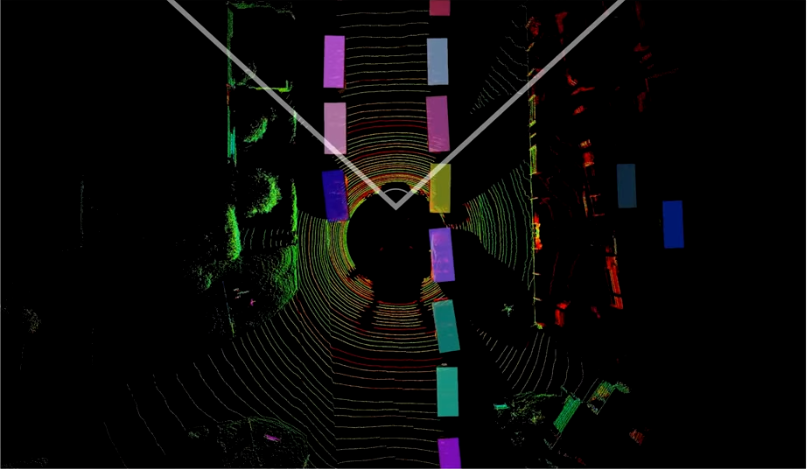
\includegraphics[width=\textwidth]{chapter_4_SmartMOT/qualitative/MOT_kitti_lidar_1.PNG}
		\caption{BEV LiDAR perspective, $t$}
	\end{subfigure}
	\hfill
	\begin{subfigure}{0.45\textwidth}
		\captionsetup{justification=centering}
		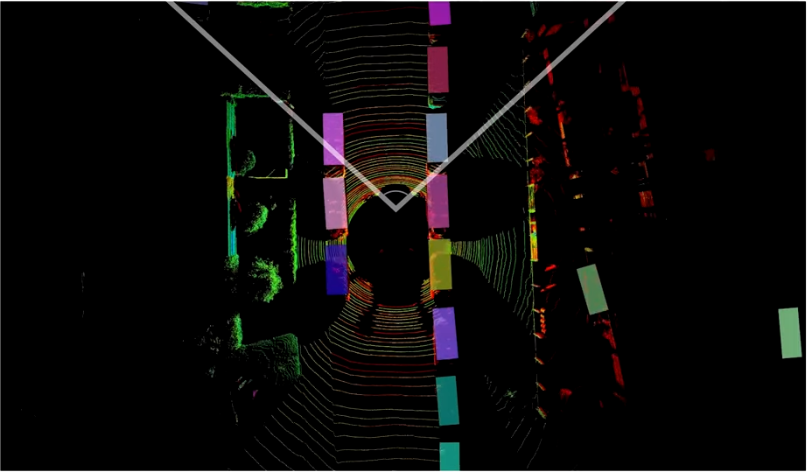
\includegraphics[width=\textwidth]{chapter_4_SmartMOT/qualitative/MOT_kitti_lidar_2.PNG}
		\caption{BEV LiDAR perspective, $t+20$}
	\end{subfigure}
	\hfill
	\begin{subfigure}{0.45\textwidth}
		\captionsetup{justification=centering}
		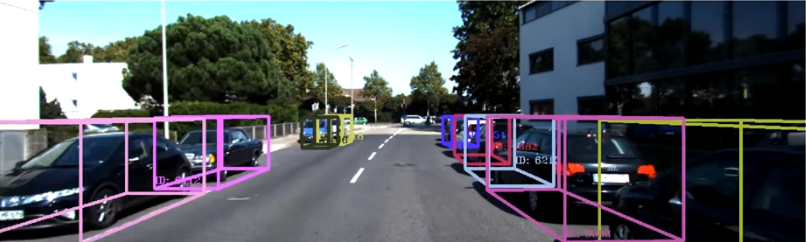
\includegraphics[width=\textwidth]{chapter_4_SmartMOT/qualitative/MOT_kitti_left_camera_1.PNG}
		\caption{Left RGB camera perspective, $t$}
	\end{subfigure}
	\hfill
	\begin{subfigure}{0.45\textwidth}
		\captionsetup{justification=centering}
		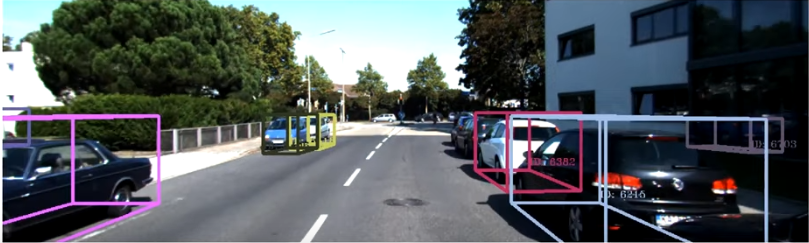
\includegraphics[width=\textwidth]{chapter_4_SmartMOT/qualitative/MOT_kitti_left_camera_2.PNG}
		\caption{Left RGB camera perspective, $t+20$}
	\end{subfigure}
	\captionsetup{justification=justified}
	\caption[SmartMOT in the KITTI \ac{MOT} validation dataset without map monitoring]{SmartMOT in the KITTI \ac{MOT} validation dataset without map monitoring. Velodyne HDL-64 is used as raw data. It can be appreciated two perspectives ((a) (b) \ac{BEV} \ac{LiDAR} and (c) (d) Left RGB camera) in frame $t$ (left column) and $t+20$ (right column).}
	\label{fig:chapter_4_SmartMOT/MOT_KITTI}
\end{figure}

Figure \ref{fig:chapter_4_SmartMOT/MOT_KITTI} illustrates the tracked agents in a standard urban scenario of the KITTI \ac{MOT} dataset in frames $t$ and $t+20$ respectively, where the Velodyne HDL-64 is used as raw data for the object detector. It may be observed how the corresponding agents are correctly estimated, compensating their position with the ego-motion. Moreover, as aforementioned, SmartMOT operates in the \ac{BEV} plane, in such a way we assume the dimensions, in particular the $z$-coordinate of the agents, are the same for the detection and the tracker.

% we reproduce a very common situation (as observed in the KITTI dataset) which is the ego-vehicle driving in narrow streets full of parked obstacles aside, evaluating its performance in night conditions. Despite this is probably the major disadvantage when using camera information (very poor performance in night conditions), we get impressive results in this situation, as illustrated in Figure \ref{fig:chapter_4_SmartMOT/MOT_CARLA}. This is pretty much coherent since LiDAR sensors are not passive sensors like cameras but they supply their own illumination source, which hits objects the reflected energy is detected and measured by the sensor in order to compute the distance to the object.

On the other hand, in terms of our real-world prototype, we focus on implementing a 360\degree~real-time and power-efficient SmartMOT pipeline in an efficient way. Perception systems in \ac{AD} must process a huge amount of information coming from at least one sensor in order to understand the environment. However, the physical space occupied by the processing units in the vehicle or their power consumption are metrics to be deeply analyzed, even more if these processing units will be integrated in an electric vehicle, where the state of the batteries is crucial. 

Regarding this, the \ac{SOTA} approach is to use powerful but power-efficient \ac{AI} embedded systems as computation devices for autonomous machines, since they present a remarkable ratio between performance and power consumption in a reduced-size hardware. In terms of the advantage of using neural networks in \ac{GPU}, these embedded systems present a powerful \ac{GPU} unit as well as fast storages based on Solid State Disks (SSDs) and a large Random Access Memory (RAM) memory size. At the time of writing this paper (2023), the best ratio of performance vs power consumption and size is represented by the NVIDIA Jetson embedded computing boards. NVIDIA Jetson is the world's leading \ac{AI} computing platform for \ac{GPU}-accelerated parallel processing in mobile embedded systems. These kits allow to implement \ac{SOTA} frameworks and libraries to conduct accelerated computing, such as \ac{CUDA}, cuDNN or TensorRT (Tensor RealTime). 

\begin{table}[h]
	\captionsetup{justification=justified}
	\caption[Comparative of inference frequency of SmartMOT between the NVIDIA Jetson AGX Xavier and our PC desktop]{Comparative of inference frequency of SmartMOT between the NVIDIA Jetson AGX Xavier and our PC desktop (Intel Core i7-9700, 16GB RAM) with CUDA-based NVIDIA GeForce RTX 1080 Ti 11GB VRAM.}
	\label{table:4_smartmot_xavier_vs_computer_hz}
	\begin{center}
		\begin{tabular}{ c | c c c}
			\toprule
			Stage & Frequency AGX $\uparrow$ &  Frequency PC $\uparrow$ & Ratio \\
			& Xavier (Hz) & desktop (Hz) & \\
			\midrule
			Detection & 7.3 & \bf{41.7} & 5.7x \\
			\hline
			Tracking & 15 & \bf{101.9} & 6.7x \\
			\bottomrule
		\end{tabular}
	\end{center}
\end{table}

In this particular work we make use of the NVIDIA Jetson AGX Xavier, one of the most powerful \ac{AI} embedded system specially designed for \acp{ADS}. Table \ref{table:4_smartmot_xavier_vs_computer_hz} shows a comparative between the embedded system and our PC frequency in the inference stage, where the detection stage (PointPillars) is reduced by almost 6 times and the tracking by almost 7 times. Nervertheless, although the detection and tracking frequencies are on the border to be considered real-time according to the requirements of the perception systems for \acp{ADS} (at least 10 Hz), the embedded system consumes 30 W whilst only the 1080 Ti GPU consumes 250 W at full power respectively. 

Considering that the embedded system computation power is reduced by 6.2 times (average between the detection and tracking frequency ratios) but only the \ac{GPU} (not considering the whole PC desktop) presents a power consumption 8.3 higher, it makes the NVIDIA Jetson AGX Xavier a better suitable option for large scale-deployment in the \ac{AD} field rather than using heavy desktop graphic cards. Distributing several sensor processing across multiple embedded systems for parallelization will result in lower power consumption than using conventional \acp{GPU} in future \ac{AD} prototypes. 

\begin{figure}[h]
	\centering
	\begin{subfigure}{0.43\textwidth}
		\captionsetup{justification=centering}
		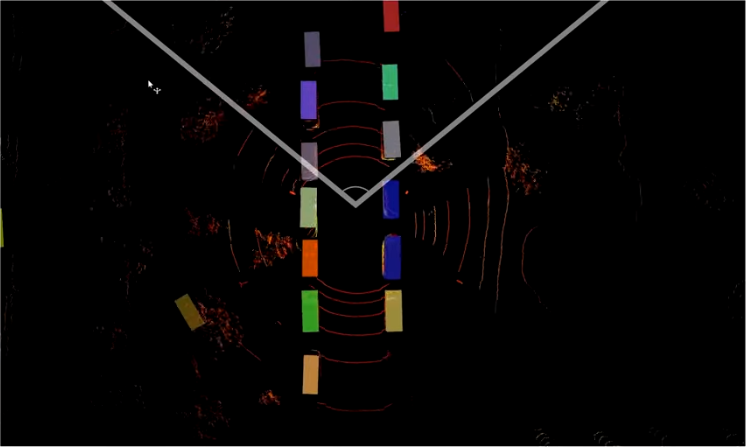
\includegraphics[width=\textwidth]{chapter_4_SmartMOT/qualitative/MOT_campus_lidar_1.PNG}
		\caption{}
	\end{subfigure}
	\hfill
	\begin{subfigure}{0.43\textwidth}
		\captionsetup{justification=centering}
		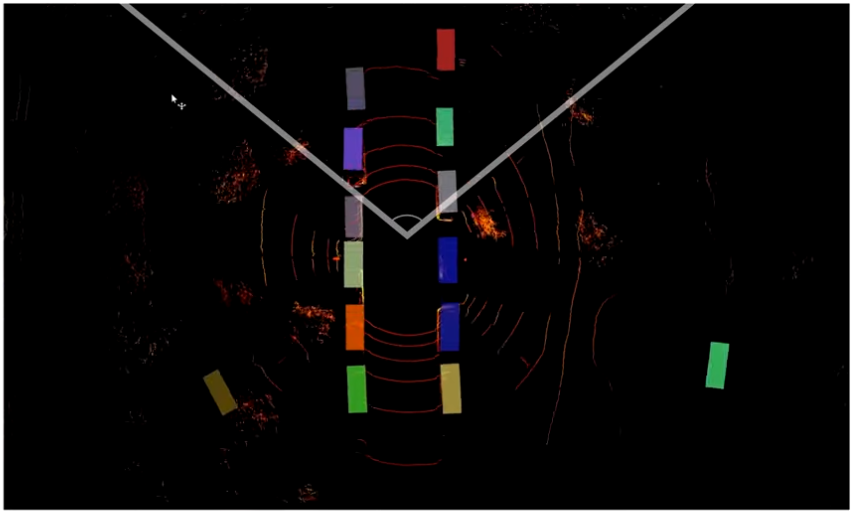
\includegraphics[width=\textwidth]{chapter_4_SmartMOT/qualitative/MOT_campus_lidar_2.PNG}
		\caption{}
	\end{subfigure}
	\hfill
	\begin{subfigure}{0.43\textwidth}
		\captionsetup{justification=centering}
		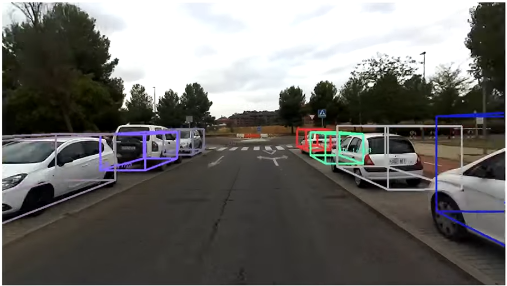
\includegraphics[width=\textwidth]{chapter_4_SmartMOT/qualitative/MOT_campus_left_camera_1.PNG}
		\caption{}
	\end{subfigure}
	\hfill
	\begin{subfigure}{0.43\textwidth}
		\captionsetup{justification=centering}
		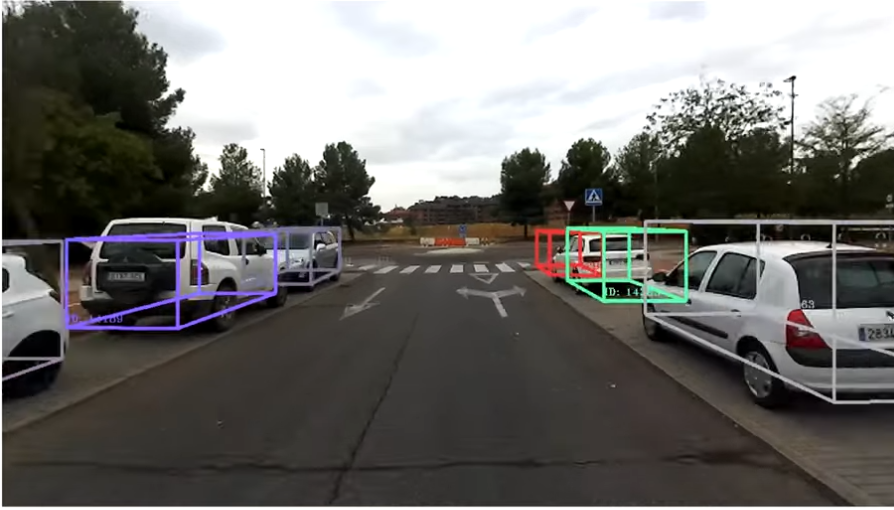
\includegraphics[width=\textwidth]{chapter_4_SmartMOT/qualitative/MOT_campus_left_camera_2.PNG}
		\caption{}
	\end{subfigure}
	\captionsetup{justification=justified}
	\caption[SmartMOT in our campus with our real-world vehicle without map monitoring]{SmartMOT in our campus with our real-world vehicle without map monitoring. Velodyne VLP-16 is used as raw sensor data. It can be appreciated two perspectives ((a) (b) BEV LiDAR and (c) (d) Left RGB camera) in frame $t$ (left column) and $t+20$ (right column).}
	\label{fig:chapter_4_SmartMOT/MOT_campus}
\end{figure}

Qualitative results of running our SmartMOT pipeline in our own vehicle, equipped with a VLP-16 \ac{LiDAR} instead of the HDL-64 shown in KITTI, are illustrated in Figure \ref{fig:chapter_4_SmartMOT/MOT_campus}. It can be appreciated that although the obtained results are slightly worse than with the KITTI dataset (equipped with a HDL-64 sensor), we obtain quite promising results, validating the pipeline studied in this work both in terms of accuracy and real-time operation.

\begin{figure}[]
	\begin{subfigure}{\textwidth}
		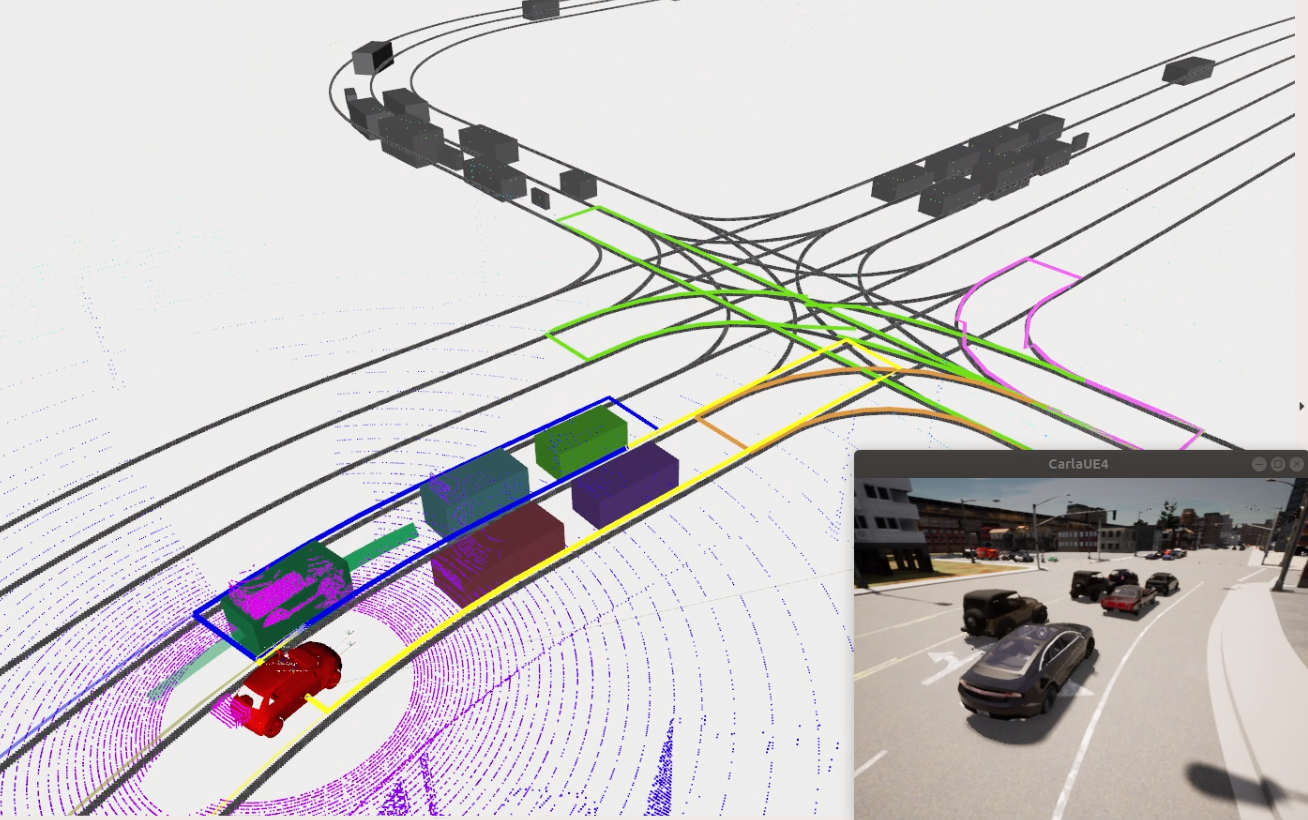
\includegraphics[width=\textwidth]{chapter_4_SmartMOT/qualitative/smartmot_CARLA_t}
		\label{subfig:chapter_4_SmartMOT/qualitative/smartmot_CARLA_t}
		\caption{Traffic scenario at frame $t$}
	\end{subfigure}
	\begin{subfigure}{\textwidth}
		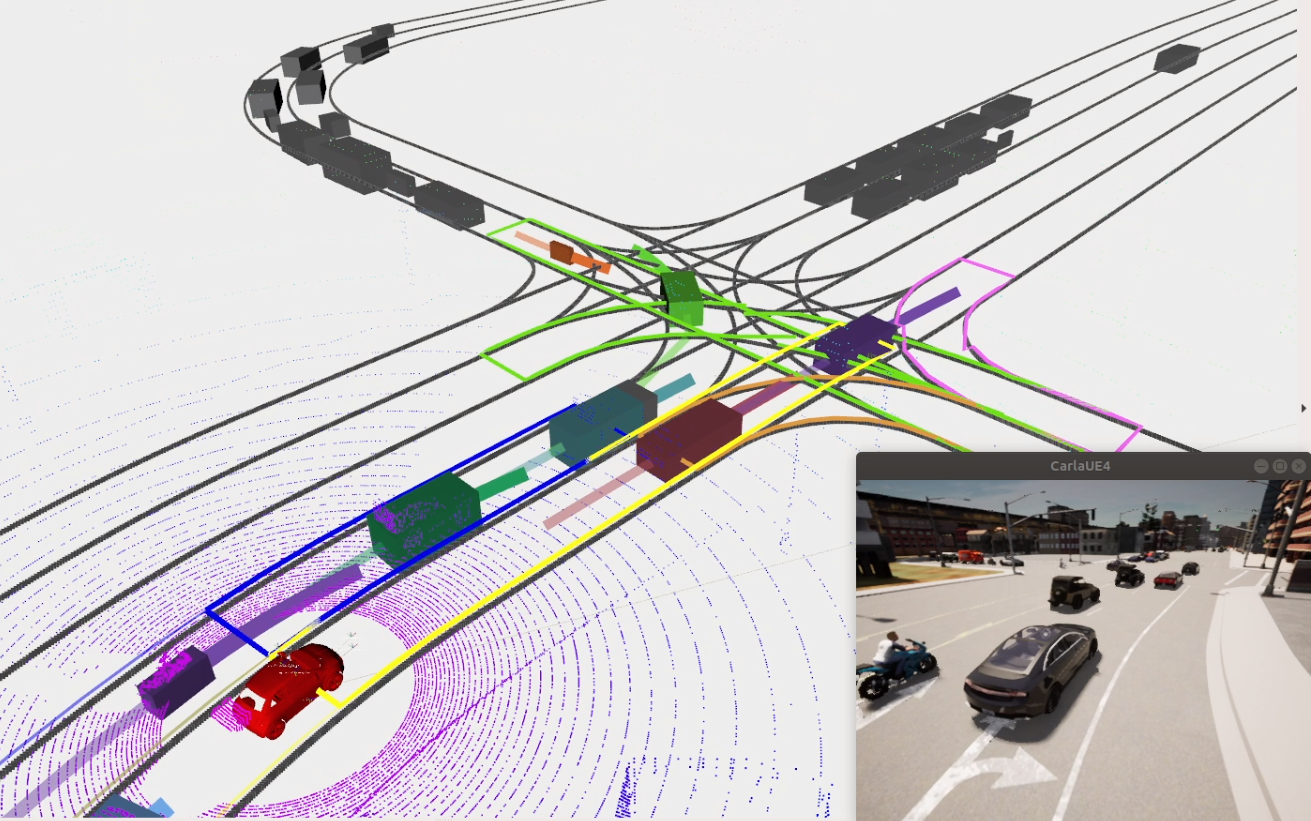
\includegraphics[width=\textwidth]{chapter_4_SmartMOT/qualitative/smartmot_CARLA_t+40.png}
		\label{subfig:chapter_8_Applications/qualitative/smartmot_CARLA_t+40}
		\caption{Traffic scenario at frame $t+40$}
	\end{subfigure}
	\captionsetup{justification=justified}
	\caption[Simulation use case processed by SmartMOT (tracking + map monitor filtering + \ac{CTRV} prediction in the \ac{CARLA} simulator)]{Simulation use case processed by SmartMOT (tracking + map monitor filtering + \ac{CTRV} prediction in the \ac{CARLA} simulator). As observed, only the most relevant objects are tracked (\ie \ those which are in the monitored area and may be relevant in the short-term for the ego-vehicle).}
	\label{fig:chapter_4_SmartMOT/SmartMOT_CARLA}
\end{figure}

Finally, we illustrate some qualitative results in \ac{CARLA} with and without the Monitored Lanes-based Attention Module to study the average inference time in several scenarios. Note that this attention module was not applied neither in the KITTI dataset (since \ac{HDmap} information is not provided here) nor in our campus with the real-world vehicle of our research group since map information was not available at the moment of conducting the different experiments. 

One of the best advantages of \ac{CARLA} is the possibility to create ad-hoc urban layouts by means of an OpenSCENARIO \cite{jullien2009openscenario} script definition where town, vehicles, climate conditions and also driving behaviours are defined, helpful to validate \ac{AD} algorithms (specially those focused on the perception layer) under different traffic and weather conditions. 

In this particular case, we design different complex 4-ways intersection in the Town03, where different lanes of interest are monitored (\ie \ current, left, merge, split and intersection). Note that we chose intersections since the number of agents and relevant lanes are noticeable higher than other traffic situations. For simplicity, in order to appreciate the full strength of SmartMOT when applying our proposed Monitored Lanes-based Attention Module, we take the detection \ac{GT} of the simulator until a given threshold (in this case, $150m$), in order to avoid the error propagated from the detection stage in real-world scenarios. Additional qualitative results may be found in \href{https://github.com/Cram3r95/SmartMOT}{SmartMOT} \footnote{https://github.com/Cram3r95/SmartMOT}.

As an example, Figure \ref{fig:chapter_4_SmartMOT/SmartMOT_CARLA} illustrates how only the agents which current positions are within the monitored area are considered as relevant detections (\ie \ agents which are on the left or right lane where a lane change maneuver is possible, agents which are within an intersection lane where there is an explicit risk of collision, etc.), noticeable reducing the average inference time throughout the route since there are way less agents to be tracked. In particular, after running the model several times in the different intersections with an average number of 30 traffic agents (located 360\degree~around the ego-vehicle) we report an average inference time of the tracking stage of 27 ms when the map monitor module is not used. This inference time makes sense since it represents a frequency of 37Hz, whilst in Table \ref{table:4_smartmot_xavier_vs_computer_hz} we illustrated a frequency of 101.9Hz with fewer detected obstacles (Figure \ref{fig:chapter_4_SmartMOT/MOT_campus}). On the other hand, considering the same experimental setup (\ie \ same traffic scenario, number of agents and platform, in our case a PC desktop (Intel Core i7-9700, 16GB RAM) with CUDA-based NVIDIA GeForce RTX 1080 Ti 11GB VRAM), when our Monitored Lanes-based Attention module is used in the SmartMOT pipeline, we are able to reduce the inference time of the overall pipeline from 27ms to an average time of 8ms (around 6 agents are considered in the monitored area), that is, about a third of the original inference time when all objects in the environment (including relevant and non-relevant) were tracked. 

In conclusions, with this experimental setup, it takes approximately 1ms to perform state estimation, data association and physics-based. The higher the number of trackers, the longer the inference time of SmartMOT since calculations are not parallelized, so our filtering process helps the overall model to avoid unnecessary calculations which will not be relevant for the ego-vehicle at least in the short-term. 

\begin{comment}
\subsection{EuroNCAP-based validation}
\label{subsec:4_euroncap}

% Check this link: https://cdn.euroncap.com/media/58230/euro-ncap-assessment-protocol-vru-v1003.pdf

A considerable amount of research works and studies, related to pedestrian detection and collision avoidance behavior are present in the literature, where the main objective is to validate the perception and control modules. Nevertheless, as stated before, we aim to demonstrate how incorporating HD map information helps the whole AD stack to anticipate faster the behaviour of the traffic participants in the corresponding traffic scenarios. Then, common metrics for all frameworks must be used to evaluate the whole architecture, where all modules are integrated. Regarding this, New Car Assessment Programs (NCAPs) protocols are introduced, evaluating the safety of vehicles for different traffic situations and Advanced Driver Assistance Systems, such as Child Occupant Protection (COP), Speed Assist Systems (SAS) or Autonomous Emergency Braking (AEB). Euro-NCAP \cite{article_EuroNCAP_2} is introduced in 1997, representing the widely most adopted performance assessment within the scope of the collaboration of European Union countries. China New Car Assessment Program (C-NCAP) \cite{article_CNCAP} is presented (2006) as a research and development benchmark for vehicle manufacturers in Asia, being most of its protocols based on Euro-NCAP. National Highway Transportation Safety Administration (NHTSA), funded in 1970 as an agency of the Department of Transportation of United States, published \cite{article_NHTSA} its guidance documents and regulations on vehicles equipped with ADAS. As observed, these programmes do not present specific protocols in order to evaluate AD stacks, presenting noticeable differences, such as different scenarios, parameters and evaluation metrics. 

Regarding this, in order to evaluate SmartMOT, we adopt the validation method proposed by \cite{gutierrez2021validation}, which proposes to generalize the \ac{VRU} v.10.0.3 protocol \cite{web_VRU_assessment_protocol}, representing a baseline to compare the performance of different pipelines for the particular situation (both in simulation and real-world) of an Unexpected Vulnerable Road User (VRU) jumping into the road during the navigation, where an Autonomous Emergency Braking (AEB) behaviour must be executed. 

\subsubsection{Implementation details of the EuroNCAP scenario}
\label{subsubsec:4_euroncap_implementation_details}

Figure \ref{fig:chapter_4_SmartMOT/CPNA_scenario} illustrates this traffic situation, in which the VRU (a pedestrian in this particular case) starts in the closest sidewalk to the vehicle in a perpendicular position to the vehicle orientation. Once the vehicle starts the navigation and the L2 distance between the ego-vehicle centroid and the VRU centroid is lower than a certain threshold \textit{d}, the VRU starts its path to unexpectedly cross the road in such a way the ego-vehicle must detect, track and forecast its future trajectory in order to avoid the collision or at least reduce the impact velocity as much as possible. Then, the protocol consists on reproducing the CPNA crash avoidance scenario, with a fixed VRU velocity (\(v_p\)) of 5 km/h and a variable ego-vehicle velocity that ranges from 10 km/h to 60 km/h. It is important to note that the threshold \textit{d} is not fixed, but it is ego-vehicle velocity dependent, that is, the pedestrian must start walking in such a way the impact point (\(P_I\)) (Figure \ref{fig:4_cpna_scenario}) is in the center of the lane for each particular velocity. 

\begin{figure}[h]
	\centering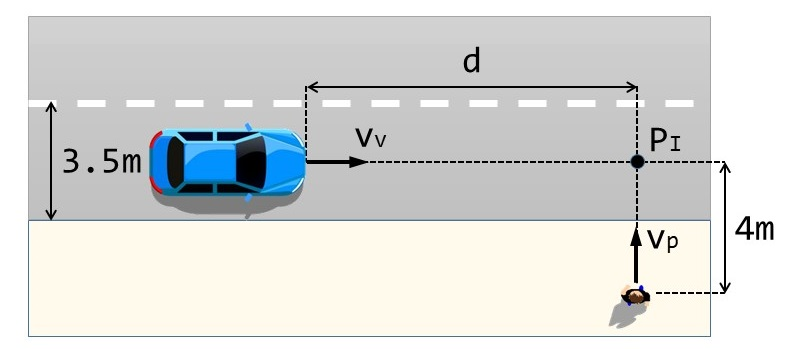
\includegraphics[width=0.4\textwidth]{chapter_4_SmartMOT/CPNA_scenario.jpg}
	\caption{Car to Pedestrian Nearside Adult (CPNA) scenario}	
	\label{fig:chapter_4_SmartMOT/CPNA_scenario}
\end{figure}

Regarding the evaluation metrics, a score for each test is calculated based on the velocity reduction of the vehicle, as following:

\begin{itemize}
	\item For a vehicle velocity \(v_v\) less than or equal to 40km/h:
	\begin{itemize}
		\item If the vehicle stops without collision, the highest score is achieved:
		\begin{equation}
			score_{test} = score_{max}
			\label{eq1}
		\end{equation}
		
		\item Otherwise, if the vehicle collides, its score is defined as follows:
		\begin{equation}
			score_{test} = \frac{v_{test}-v_{impact}}{v_{test}} \cdot score_{max}
			\label{eq2}
		\end{equation}
	\end{itemize}
	\item For \(v_v\) higher than 40km/h:
	\begin{itemize}
		\item If the vehicle is able to reduce its speed in at least 20 km/h, the highest score is achieve:
		\begin{equation}
			v_{impact} \leq v_{test} - 20 \to score_{test} = score_{max}
			\label{eq3}
		\end{equation}
		\item Otherwise, if the vehicle collides at a velocity greater than the velocity under test less a threshold of 20 km/h, no score is achieve:
		\begin{equation}
			v_{impact} > v_{test} - 20 \to score_{test} = 0
			\label{eq4}
		\end{equation}
	\end{itemize}
\end{itemize}

Finally, the final score of a particular pipeline is given by the arithmetic mean of the results obtained in each CPNA crash avoidance test for different weather conditions. For further details about the validation protocol, we refer the reader to \cite{gutierrez2021validation}.

\subsubsection{Experimental results in the EuroNCAP-based scenario}
\label{subsubsec:4_euroncap_experimental_results}

In this section we obtain some interesting both qualitative and quantitative results, evaluating our AD stack \cite{gomez2021train} in the CPNA crash avoidance scenario using two different perception layer strategies. On the one hand, we implement the perception module stated by \cite{gomez2020real} which tracks all objects in the environment regardless their topological information and considers a naive velocity dependent rectangular monitored area in front of the vehicle to determine the distance to the nearest object in the route as well as to predict the collision. On the other hand, we use SmartMOT to track and predict the future trajectories of only the most relevant obstacles around the vehicle, that is, those in which the human in manual driver should pay attention throughout the route, such as VRUs close to the road, vehicles in intersections and lanes where the lane change maneuver is allowed, etc. Qualitative results may be found in the following play list \href{https://cutt.ly/uk9ziaq}{SmartMOT} \footnote{SmartMOT: https://cutt.ly/uk9ziaq}, where the SmartMOT performance is illustrated. 

Regarding urban environment complexity, in order to validate a whole AD architecture the system must be tested in countless environments and scenarios, which would escalate the cost and development time exponentially with a physical approach. Considering this, the use of photo-realistic simulation (virtual development and validation testing) and an appropriate design of the driving scenarios are the current keys to build safe and robust AV. 

In our work we propose the use of CARLA (CAR Learning to Act) \cite{dosovitskiy2017carla} as the best open-source simulator to reach our goals, taking even more importance when analyzing the behaviours the vehicle can face in these complex traffic scenarios. One of the best advantages of CARLA is the possibility to create ad-hoc urban layouts, useful to validate the navigation architecture in challenging driving scenarios. This code can be downloaded from the ScenarioRunner repository, associated to the CARLA GitHub. The ScenarioRunner is a module that allows the user to define and execute traffic scenarios for the CARLA simulator. In the present case, we define several scenarios according to the CPNA crash avoidance traffic situation, modifying the velocity of the ego-vehicle and the presence of other traffic participants. All test were carried out in a PC desktop (Intel Core i7-9700k, 32GB RAM with CUDA-based NVIDIA GeForce RTX 2080 Ti 11GB VRAM), using the version 0.9.10.1 version of CARLA as well as the corresponding ROS Bridge, responsible of communicating the CARLA environment with our ROS-based architecture, and ScenarioRunner modules. In particular, we make use of the OpenScenario standard, supported by ScenarioRunner, where both the VRU and ego-vehicle features can be modified to accomplish the Euro-NCAP requirements. % Due to size constraint of this paper, we do not validate the performance of our architecture for different weather conditions but only in daytime conditions. 

\begin{figure}[h]
	\centering
	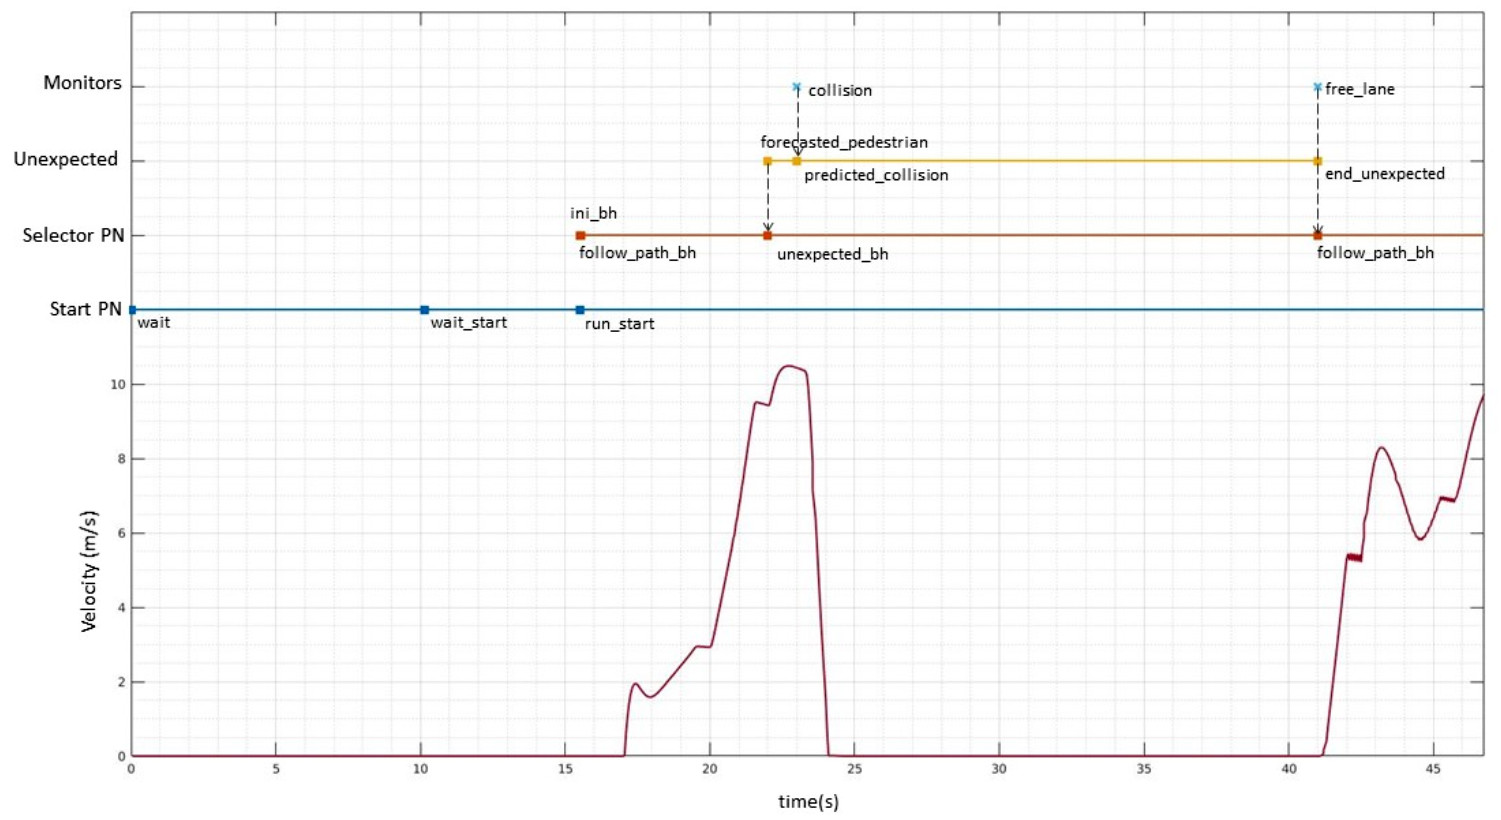
\includegraphics[width=0.8\textwidth]{chapter_4_SmartMOT/quantitative/unexpected_vru_temporal_graph.jpg}
	\captionsetup{justification=justified}
	\caption[Unexpected Vulnerable Road User (VRU) temporal diagram]{Unexpected Vulnerable Road User (VRU) temporal diagram. At the top, the events produced by our monitors and map manager modules. In the middle, the selector, and start (background) PNs of our decision-making layer. At the bottom, the velocity of the car throughout the navigation}
	\label{fig:chapter_4_SmartMOT/quantitative/unexpected_vru_temporal_graph}
\end{figure}

In order to appreciate the behaviour of the vehicle during navigation, we incorporate an illustrative temporal diagram (Figure \ref{fig:chapter_4_SmartMOT/quantitative/unexpected_vru_temporal_graph}), representing a powerful manner to qualitatively validate how the architecture behaves in an end-to-end manner, since we can observe how the car behaves considering the different actions and events \cite{gomez2021train} provided by the executive layer, which is actually the output of the whole architecture before sending commands to the motor. As observed, the ego-vehicle starts far away from the adversary and starts its navigation. At second 22 a pedestrian that is in the sidewalk is detected, so tracking-by-detection and subsequent motion prediction must be carried as fast as possible to avoid collision, since the scenario is designed in such a way that the pedestrian must start walking in such a way the impact point (\(P_I\)) (Figure \ref{fig:chapter_4_SmartMOT/CPNA_scenario}) is in the center of the lane for each particular velocity. After that, our prediction module intersects the ego-vehicle forecasted trajectory and the pedestrian forecasted trajectory. If the Intersection over Union (IoU) is greater than a threshold (in this case, 0.01), a \textit{predictedcollision} flag is activated and the low-level (reactive) control, which always runs in the background of the decision-making layer, performs an emergency break until the car is stopped in front of the obstacle. Navigation is resumed once the obstacle leaves the driving lane. Table \ref{table:4_CPNA_results} compares the performance of the architecture by implementing \cite{gomez2020real} and a rectangular monitorized lane to retrieve the nearest object in route and predict collision against our proposal, where it can be appreciated that for velocities greater than 40 km/h, using HD map semantic and geometric information gives the car a valuable reaction time to anticipate the VRU behaviour and avoid the collision, achieving the highest score. 

\begin{table}[h]
	\centering
	\captionsetup{justification=justified}
	\caption{Comparison of our two different perception strategies in the Car to Pedestrian Nearside Adult (CPNA) scenario. We bold the best score in \textbf{black}.}
	\label{table:4_CPNA_results}
	\begin{tabular}{c | c | c  c | c  c  } 
		\toprule 
		\multicolumn{6}{c}{\textbf{CPNA}}\\
		\multirow{2}{*}{\textbf{\(v_{test}\)}} & \multirow{2}{*}{\textbf{\(score_{max}\)}} & \multicolumn{2}{c}{\textbf{Rectangular area + \cite{gomez2020real}}} & \multicolumn{2}{c}{\textbf{SmartMOT}} \\ 
		& & \(v_{impact}\) & \(score\) & \(v_{impact}\) & \(score\) \\
		\midrule
		10 km/h & 1.00 & 0.0 km/h & 1.00 & 0.0 km/h & 1.00 \\
		20 km/h & 1.00 & 0.0 km/h & 1.00 & 0.0 km/h & 1.00 \\
		30 km/h & 2.00 & 0.0 km/h & 2.00 & 0.0 km/h & 2.00 \\
		40 km/h & 3.00 & 0.0 km/h & 3.00 & 0.0 km/h & 3.00 \\
		50 km/h & 2.00 & 23.82 km/h & 2.00 & 0.0 km/h & 2.00 \\
		60 km/h & 1.00 & 44.23 km/h & 0.00 & 0.0 km/h & 1.00  \\
		\midrule
		\textbf{Total} & 10.00 &  & 9.00 & & \textbf{10.0} \\
		\bottomrule
	\end{tabular}
\end{table}

Figure \ref{fig:4_cpna_results} shows different analysis of the CPNA crash avoidance scenario with variable ego-vehicle and the incorporation of other traffic participants in the scenario (\ref{subfig:chapter_4_SmartMOT/euroncap_graphics_c} \ref{subig:chapter_4_SmartMOT/euroncap_graphics_d}). \(T_0\) corresponds with the moment the vehicle either stops or collides, and crosses \textbf{x} represent the moment in which the system sends a predicted collision signal to the executive layer, so it is coherent that crosses in tests where the ego-vehicle collides with the VRU are shifted to the right (prediction collision signal was given in time). Left column tracks all objects around the vehicle and adopts a geometric monitorized area to estimate the nearest distance and predicted collision, whilst right column uses HD map information to help in the Multi-Object Tracking and motion prediction tasks, monitoring only the most relevant traffic participants around the vehicle that is, the main purpose of SmartMOT.

As observed, using HD map information is able to avoid collision until a ego-vehicle velocity of 80 km/h, where SmartMOT is not able to send a signal of predicted collision (output of the system, as shown in Figure \ref{fig:chapter_4_SmartMOT/IV_2021}) in time, colliding at a velocity of 39.78 km/h. Nevertheless, this velocity at the moment of collision is even lower that the impact velocity (44.23 km/h) when testing the system under 60 km/h condition not using HD map in the MOT stage, illustrating how incorporating additional semantic and geometric map information helps the vehicle to react faster or at least mitigate the effect of collision. Moreover, we simulate both perception strategies using the most common velocities in urban scenarios, which range from 30 to 50 km/h, including \ref{subfig:chapter_4_SmartMOT/euroncap_graphics_c} \ref{fig:chapter_4_SmartMOT/euroncap_graphics_d} static adversaries (in particular, vehicles and pedestrians) which do not actually in the traffic scenario to fulfill the particular requirements stated by \cite{gutierrez2021validation} protocol. As expected, tracking all objects around the ego-vehicle and using the rectangular monitorized area suffers when the number of traffic participants is increased around the ego-vehicle, whilst SmartMOT holds this exponential increase by analyzing the objects and their corresponding role as relevant obstacles considering the information provided by the HD map, avoiding the collision in all situations.

\begin{figure}[h]
	\centering
	\begin{subfigure}{0.45\textwidth}
		\includegraphics[width=\textwidth]{chapter_4_SmartMOT/quantitative/euroncap_without_adversaries_geometric.jpg}
		\caption{Rectangular monitored area without adversaries}
		\label{subfig:chapter_4_SmartMOT/euroncap_graphics_a}
	\end{subfigure}
	\hfill
	\begin{subfigure}{0.45\textwidth}
		\includegraphics[width=\textwidth]{chapter_4_SmartMOT/quantitative/euroncap_without_adversaries_hdmap.jpg}
		\caption{SmartMOT area without adversaries}
		\label{subfig:chapter_4_SmartMOT/euroncap_graphics_b}
	\end{subfigure}
	\hfill
	\begin{subfigure}{0.45\textwidth}
		\includegraphics[width=\textwidth]{chapter_4_SmartMOT/quantitative/euroncap_with_adversaries_geometric.jpg}
		\caption{Rectangular monitored area with adversaries}
		\label{subfig:chapter_4_SmartMOT/euroncap_graphics_c}
	\end{subfigure}
	\hfill
	\begin{subfigure}{0.45\textwidth}
		\includegraphics[width=\textwidth]{chapter_4_SmartMOT/quantitative/euroncap_with_adversaries_hdmap.jpg}
		\caption{SmartMOT area with adversaries}
		\label{subfig:chapter_4_SmartMOT/euroncap_graphics_d}
	\end{subfigure}
	\captionsetup{justification=justified}
	\caption[Analysis of the Car to Pedestrian Nearside Adult (CPNA) crash avoidance scenario with variable ego-vehicle velocity]{Analysis of the Car to Pedestrian Nearside Adult (CPNA) crash avoidance scenario with variable ego-vehicle velocity. Left column (Figures \ref{subfig:chapter_4_SmartMOT/euroncap_graphics_a} and \ref{subfig:chapter_4_SmartMOT/euroncap_graphics_c}) adopts a rectangular monitorized area to estimate the nearest distance and predicted collision, Right column (Figures \ref{subfig:chapter_4_SmartMOT/euroncap_graphics_b} and \ref{subfig:chapter_4_SmartMOT/euroncap_graphics_d}) uses HD map information for this purpose. On the other hand, first row shows the scenario without additional traffic participants, second row analyzes the crash avoidance scenario including additional traffic participants to the road, monitorized sidewalk area and non-relevant sidewalk area. Crosses in the lines represent the moment in which the system sends a predicted collision signal to the executive layer}
	\label{fig:4_cpna_results}
\end{figure}

\end{comment}

\section{Summary}
\label{sec:4_summary}

In this Chapter we propose SmartMOT, an open-source simple-yet-powerful pipeline that fuses the concepts of tracking-by-detection and \ac{HDmap} information to design a real-time and power-efficient \ac{MOT} and uni-modal \ac{MP} pipeline used to track and predict the future trajectories of only the most relevant obstacles around the ego-vehicle, incorporating a Monitored Lanes-based Attention Module to the pipeline, improving the way in which the vehicles are considered as relevant.

Then, experimental results focus on validating the tracking stage (without including map monitoring) in the KITTI dataset where the Velodyne HDL-64 is used, performing an ablation study to choose the final hyperparameters of the proposal. This proposal is also validated using data captured from our \ac{LiDAR} using a Velodyne VLP-16, obtaining successful qualitative results since we do not have \ac{GT} in this case. On top of that, we run the pipeline in a PC desktop and the Jetson NVIDIA AGX Xavier mounted in our real-world vehicle, concluding that even though the PC desktop presents a higher inference frequency, the higher ratio compared to the power consumption saved when using the edge computing device is lower. In that sense, in spite the fact that its integration is more difficult due to the distribution of several sensor processing across multiple embedded systems for parallelization, multiple edge-computing devices will be a preferred option rather than using heavy PC desktops and \ac{GPU} in future \ac{AD} prototypes. 

Finally, the Chapter illustrates some results in \ac{CARLA}, including map monitor information, where it can be clearly appreciated how tracking the most relevant agents of the scene (\ie \ those which are included in the monitored area) can drastically reduce the inference time, making it suitable for real-time classic \ac{MOT} and uni-modal \ac{MP} operation, where no learning-based methods are required to reason what is happening in the traffic scenario, both in terms of physical and social information.

%Once the best hyperparameters are obtain by means of an ablation study, an end-to-end validation of our pipeline in the Unexpected \ac{VRU} scenario is carried out, following an Euro-NCAP-based validation protocol, illustrating how integrating map information in the pipeline can minimize or at least reduce the impact velocity with the \ac{VRU} by reducing the computational complexity of the problem. Moreover, a temporal graph is depicted, representing a very intuitive and powerful manner to appreciate how the integration of this extended version of SmartMOT gives the vehicle a valuable time to anticipate the corresponding behaviours. We hope that our distributed pipeline can serve as a solid baseline on which others can build on to advance the state-of-the-art in fusing perception data and map information to perform real-time motion prediction and decision-making evaluation in arbitrarily complex urban scenarios. 
%%%%%%%%%%%%%%%%%%%%%%%%%%%%%%%%%%%%%%%%%%%%%%%%%%%%%%%%%%%%%%%%%%%%%%%%%%% 
% 
% Generic template for TFC/TFM/TFG/Tesis
% 
% By:
% + Javier Macías-Guarasa. 
% Departamento de Electrónica
% Universidad de Alcalá
% + Roberto Barra-Chicote. 
% Departamento de Ingeniería Electrónica
% Universidad Politécnica de Madrid   
% 
% Based on original sources by Roberto Barra, Manuel Ocaña, Jesús Nuevo,
% Pedro Revenga, Fernando Herránz and Noelia Hernández. Thanks a lot to
% all of them, and to the many anonymous contributors found (thanks to
% google) that provided help in setting all this up.
% 
% See also the additionalContributors.txt file to check the name of
% additional contributors to this work.
% 
% If you think you can add pieces of relevant/useful examples,
% improvements, please contact us at (macias@depeca.uah.es)
% 
% You can freely use this template and please contribute with
% comments or suggestions!!!
% 
%%%%%%%%%%%%%%%%%%%%%%%%%%%%%%%%%%%%%%%%%%%%%%%%%%%%%%%%%%%%%%%%%%%%%%%%%%% 

\chapter{Exploring GAN for Vehicle Motion Prediction}
\label{cha:exploring_gan_for_vehicle_mp}

\begin{FraseCelebre}
	\begin{Frase}
		Avanzad, sin temor a la oscuridad. \\
		Luchad jinetes de Theoden. \\
		Caerán las lanzas, se quebrarán los escudos. \\
		Aún restará la espada. \\
		Rojo será el día, hasta el nacer del sol. \\
		Cabalgad, cabalgad, cabalgad hacia la desolación \\ 
		y el fin del mundo. Muerte, muerte, muerte.
	\end{Frase}
	\begin{Fuente}
		Discurso de Theoden, Rey de Rohan \\
		El Señor de los Anillos: El Retorno del Rey
	\end{Fuente}
\end{FraseCelebre}

\section{Introduction}
\label{sec:5_introduction}

Despite the fact that SmartMOT illustrates a simple-yet-powerful tracking and prediction pipeline, traditional methods for \ac{MP} in the field of \ac{AD} are based on physical kinematic constraints and road map information with handcrafted rules. Though these approaches are sufficient in many simple situations (\ie \ vehicles moving in constant velocity or straightforward intersections), they fail to capture the rich behavior strategies and interaction in complex scenarios, in such a way they are only suitable for simple prediction scenes and short-time prediction tasks \cite{huang2022survey}. In that sense, as commented in Chapter \ref{sec:2_dl_based_mp}, recently \ac{DL} based methods have dominated this task and they usually follow an encoder-decoder paradigm. 

The main challenge in the \ac{MP} is the human driver behaviour can neither be modeled and consequently predicted properly, specially in negotiating situations \cite{gomez2021train} \cite{mercat2020multi} with many participants where considering agent-environment/agent-agent interactions \cite{sadeghian2019sophie} plays a determinant role. Then, resulting trajectories may not be necessarily feasible, not covering the full spectrum of possible trajectories that a vehicle can take. In that sense, a more natural way of capturing the feasible directions \cite{dendorfer2020goal} is to first compute a set of intermediate target points from a distribution of acceptable positions. 

In this chapter we explore the influence of attention mechanisms in generative models, in particular based on \ac{GAN} \cite{goodfellow2020generative}, to carry out the task of motion prediction. Our model considers both physical context, computing acceptable target points from the driveable area around the target agent, and social context, \ac{LSTM} \cite{hochreiter1997long} based encoder as input to a Multi-head self-attention module, as input of our generator, which combines the scene understanding around the agent vehicle (target agent to predict its trajectory) and the corresponding noise vector associated to generative models to compute the trajectories using a LSTM decoder, as illustrated in Figure \ref{fig:chapter_5_GAN/ITSC_2022}. In this context, the discriminator is applied in order to force the generator model to produce more realistic samples (\ie \ trajectories), hence, to improve the performance. 

Prior knowledge on \ac{MP} in pedestrian datasets like ETH \cite{pellegrini2009you} or UCY \cite{lerner2007ucydata} usually focuses on deep methods such as \acp{LSTM} \cite{hochreiter1997long} and \acp{GAN} \cite{goodfellow2020generative}. SocialLSTM \cite{alahi2016social} proposes an \ac{LSTM}-based model that can jointly predict the paths of all agents in the scene taking into account the common sense rules and social conventions using a social-pooling module. SocialGAN \cite{gupta2018social} enhances SocialLSTM with a generative adversarial framework, introducing a variety loss that encourage the network to cover the space of plausible paths and proposing a novel pooling global social pooling vector that encodes the subtle cues for all agents involved in the scene. SoPhie \cite{sadeghian2019sophie} considers not only the path history of all agents but also the physical context information (captured by a top-view static image, computing salient regions of the scene), combining physical and social attention mechanisms in order to help the model knows what to extract and where to focus. Goal-GAN \cite{dendorfer2020goal} predicts the most likely goal points of the agent of interesting, estimating a set of trajectories towards these potential future candidates using both physical and social context, as proposed by \cite{sadeghian2019sophie}. On the other hand, in the context of vehicle prediction \cite{chang2019argoverse, caesar2020nuscenes}, prior information takes more importance regarding the risk at certain velocities in urban / highway environments in order to perform safe navigation.

As stated in Chapter \ref{sec:2_dl_based_mp}, HD maps have been widely adopted to provide a preliminary raw physical context and then apply data-driven approaches. Recent learning-based approaches \cite{hong2019rules, casas2018intentnet}, which present the benefit of having probabilistic interpretations of different behaviour hypotheses, require to build a representation to encode the trajectory and map information. \cite{hong2019rules} assumes that detections around the vehicle are provided and focuses its work on behaviour prediction by encoding entity interactions with ConvNets. Intentnet \cite{casas2018intentnet} proposes to jointly detect traffic participants (mostly focused on vehicles) and predict their trajectories using raw LiDAR pointcloud and rendered HD map information. PRECOG \cite{rhinehart2019precog} aims to capture the future stochasiticity by flow-based generative models. Furthermore, MultiPath \cite{chai2019multipath} uses ConvNets as encoder and adopts pre-defined trajectory anchors to regress multiple possible future trajectories. 

Furthermore, as commented in previous sections, in a similar way to humans that pay more attention to close obstacles, people walking towards them or upcoming turns rather than considering the presence of people or building far away, the perception layer of a self-driving car must be modelled to focus more on the more relevant features of the scene. Social Attention is a mechanism that allows selective interactions within relevant agents. SoPhie \cite{sadeghian2019sophie} computes a different context vector for each agent, in such a way other agents features are sorted in terms of their relative distance to the agent of interest. Then, a soft attention mechanism is used to compute a context feature vector, which represents the social context. Nevertheless, a fixed size ($N_{\text{max}}$ agents) list that considers the context of all agents is sensitive to small variations \cite{mercat2020multi} of other agents positions. In that sense, SocialWays \cite{amirian2019social} presents a hand-crafted relative geometric feature to produce a set of normalized weights, in such a way the context vector represents a convex sum of other feature vectors (context of each agent) that is invariant to the ordering. 

However, these attention mechanisms were not designed to model complex interactions, no more than angles and distances due to the inherent problem of pedestrian prediction, in such a way we must find this challenging interactions in the vehicle motion prediction task to account for specific behaviours like overtaking, Adaptive Cruise Control (ACC), emergency braking or yielding. GRIP \cite{li2019grip} proposes a graph representation of vehicle neighbours, taking into account local interactions with vehicles that are closer to the target agent than a threshold distance \textit{d}.

\cite{vemula2018social} use a dot product attention module (inspired from the attention mechanism proposed by \cite{vaswani2017attention} for sentence translation), allowing joint forecast of every agent in the scene without spatial limitations, considering long range interactions regardless the ordering of the input vehicles tracks and the number of vehicles. Moreover, \cite{vemula2018social} combines this dot product with a spatio-temporal graph representation to take into account temporal and spatial dependencies of the agents, such as their absolute/relative positions and time step movements. \cite{mercat2020multi} present a multi-head extension of this dot attention mechanism, where each agent is embedded by means LSTMs before computing the dot product attention in order to produce social interactions. 

\section{Attention-based GAN}
\label{sec:5_attention_gan}

In this work, we aim to develop a model \cite{gomez2022exploring} that can successfully predict plausible future trajectories in the context of vehicle prediction, taking into account not only the past trajectory of the corresponding agent but also the past state of the most relevant obstacles around it and HD map information to compute a set of acceptable target points representing the physical constraints for our problem.

When vehicles drive through a traffic scenario, they usually aim to reach partial goals, depending on their predefined navigation route and scene context (both physical and social), until they finally arrive at their final destination. Formally, given a certain goal, vehicles must face different traffic rules and other agents along their way to reach their final destination. Regarding this, our model computes both the social context and acceptable target points for the corresponding agent given its past trajectory and then generates plausible trajectories towards the estimated goals. As illustrated in Figure \ref{fig:chapter_5_GAN/ITSC_2022}, our model consists of three main blocks:

\begin{itemize}
	\item \textit{Target Points Extractor}: Combines HD Map information and dynamic features of the target agent (speed and orientation) to generate acceptable target points in the driveable area.
	\item \textit{Attention module}: Computes the agents dynamic features recursively by means a \ac{LSTM} unit and capture complex social interactions among agents by means of Multi-Head Self Attention.
	\item \textit{GAN module}: Given the target points and highlighted social features, this module generates plausible and realistic trajectories using a LSTM based decoder, which represents the generator. Discriminator is applied to enhance the performance of the generator by forcing it to compute more realistic predictions.
\end{itemize} 

\begin{figure}[h] 
	\centering
	\includegraphics[width=\textwidth]{chapter_5_GAN/ITSC_2022.pdf}
	%\captionsetup{justification=justified}
	\caption{Overview of our Attention-based Generative model}
	\label{fig:chapter_5_GAN/ITSC_2022}
\end{figure}

Figure \ref{fig:chapter_5_GAN/ITSC_2022} illustrates an overview of our model. Next, we describe the different blocks of our model.

\subsection{Target points extraction}
\label{subsec:5_target_points_extraction}

Multiple approaches have tried to predict realistic trajectories by means of learning physically feasible areas as heatmaps or probability distributions of the agent future location \cite{dendorfer2020goal, sadeghian2019sophie, gilles2021home}. These approaches require either a top-view RGB BEV image of the scene, or a HD Map with exhaustive topological, geometric and semantic information (commonly codified as channels). This information is usually encoded using a CNN and fed into the model together with the social agent information \cite{dendorfer2020goal, sadeghian2019sophie, gao2020vectornet}.

In our model, we propose to estimate the range of motion (360º) using a minimal HD Map representation that includes only the feasible area, where we can discretize the feasible area $\mathcal{F}$ (represented by a discrete grid of the \textit{width} x \textit{height} BEV map image where the pixels are driveable) as a subset of $r$ randomly sampled points $\{p_0 , p_1 ... p_r\}$ from such area in the map (easy to extract from a 1-channel binarized HD image) considering the orientation and velocity in the last observation frame for the agent. This step can be considered as pre-processing of the HD Map, therefore the model never sees the HD map image nor the whole graph of nodes. 

\begin{figure}[!ht]
	\centering
	\begin{subfigure}{0.24\textwidth}
		\includegraphics[width=\textwidth]{chapter_5_GAN/filtering_process_1_agent_trajectory.png}	
		\caption{}
	\end{subfigure}
	\hfill
	\begin{subfigure}{0.24\textwidth}
		\includegraphics[width=\textwidth]{chapter_5_GAN/filtering_process_2_feasible_area_discretization.png}
		\caption{}
	\end{subfigure}
	\hfill
	\begin{subfigure}{0.24\textwidth}
		\includegraphics[width=\textwidth]{chapter_5_GAN/filtering_process_3_non_holonomic_filter.png}
		\caption{}
	\end{subfigure}
	\hfill
	\begin{subfigure}{0.24\textwidth}
		\includegraphics[width=\textwidth]{chapter_5_GAN/filtering_process_4_multimodal_clustering.png}
		\caption{}
	\end{subfigure}
	\captionsetup{justification=justified}
	\caption[Target Points Estimation from the Feasible area process]{Target Points Estimation from the Feasible area process: (a): Agent Past Trajectory (\textcolor{blue}{past observations} and \textcolor{aqua}{ground-truth}), (b) Feasible area discretization (random points in the driveable area), (c) Non-holonomic-based dynamic filter (both angle and velocity), (d) Multimodal clustering to get the final proposals}
	\label{fig:chapter_5_GAN/target_points_extraction}
\end{figure}

Figure \ref{fig:chapter_5_GAN/target_points_extraction} summarizes step-by-step the whole process. First, we calculate the driveable area (white area in Figure \ref{fig:chapter_5_GAN/target_points_extraction}) around the vehicle considering a hand-defined \textit{d} threshold.

Then, we consider the dynamic features of the agent of interest in the last observation frame $t_{obs}$ to compute acceptable target points in local coordinates. As we will detail in future sections, the Argoverse 1 Motion Forecasting dataset focuses on estimating the future prediction of a particular target agent. On top of that, the aforementioned dynamic features (orientation and velocity) are not provided, in such a way they must be calculated. Since the trajectory data are noisy with tracking errors, as expected from a real-world dataset, simply interpolating the coordinates between consecutive time steps, assuming constant frequency, results in noisy estimation. Then, in order to estimate the orientation and velocity of the target agent in the last observation frame $t_{obs}$, we compute a vector for each feature given:

\begin{equation}
	\begin{split}
		\theta_{i}=\arctan{(\frac{y_{i}-y_{i-1}}{x_{i}-x_{i-1}})} \\
		v_{i}=\frac{X_{i}-X_{i-1}}{t_{i}-t_{i-1}} 
	\end{split}
\end{equation}
 
where $X_{i}$ represents the 2D position of the agent at each observed frame $i$ as state above. Once both vectors are computed, we obtain a smooth estimation as proposed by \cite{tang2021exploring} of the heading angle (orientation) and velocity by assigning less importance (higher forgetting factor) to the first observations, in such a way immediate observations are the key states to determine the current spatio-temporal variables of the agent, as depicted in Equation \ref{eq:5_dynamic_feats_last_observation_frame}, which applies to both the orientation and velocity vector: 

\begin{equation}
	\hat{\psi}_{T_h} = \sum_{t=0}^{T_h}\lambda^{T_h - t}\psi_t
	\label{eq:5_dynamic_feats_last_observation_frame}
\end{equation}

where $T_h$ is the number of observed frames, $\psi_t$ is the estimated orientation/velocity at the $t_{i}$ frame, $\lambda\in(0, 1)$ is the forgetting factor, and $\hat{\psi}_{t_obs}$ is the smoothed orientation/velocity estimation at the last observed frame. After estimating these variables, we calculate the range of motion around the target agent as a circle with radius: $H * \psi_{v}$ where $\psi_{v}$ is the estimated velocity using Equation \ref{eq:5_dynamic_feats_last_observation_frame} and $H=3$ is the time-horizon of 3s. After that, we randomly sample $r$ points $p \in \mathcal{F}$ in this range considering a constant velocity model during the prediction horizon and the estimated orientation, assuming non-holonomic constraints \cite{triggs1993motion}, which are inherent of standard road vehicles, that is, the car has three degrees of freedom, its position in two axes and its orientation, and must follow a smooth trajectory in a short-mid term prediction. Finally, we estimate $k$ target points (one per mode required in the future prediction) by means of the k-means \cite{ahmed2020k} clustering algorithm. 

This clustering method, originally from signal processing, that aims to partition n observations into k clusters in which each observation belongs to the cluster with the nearest mean (cluster centers or cluster centroid), serving as a prototype of the cluster. In this particular model, we focus on unimodal prediction, that is, the model must reason the most plausible future trajectory based on the agents past observations, attention-based social interaction and target points as physical context.

This representation not only reunites information about the feasible area around the agent, but also represents potential \textbf{Target points} \cite{dendorfer2020goal} (\ie \ potential destinations or end-of-trajectory points for the agents). Moreover, this information is \textit{"cheap"} and \textit{interpretable}, therefore, we do not need further exhaustive annotations from the HD Map in comparison with other methods like HOME, which gets as input a 45-channel encoded map \cite{gilles2021home}.

We concatenate this information, as 2D vector $\mathcal{V}$, together with the model social context features to generate more realistic trajectories (see Figure \ref{fig:chapter_5_GAN/ITSC_2022}).

\subsection{Attention module}
\label{subsec:5_attention_module}

Multiple methods \cite{liang2020learning, schmidt2022crat} consider only the vehicles that are observable at \textit{t=0}, handling those agents that are not observed over the full sequence spectrum (observation length = \textit{$obs_{len}$} + prediction length = \textit{$pred_{len}$}) by concatenating a binary flag $b_i^t$ that indicates if the agent is padded or not. 

In our case, we consider the agents that have information over the full history horizon $T_h$ = \textit{$obs_{len}$} + \textit{$pred_{len}$} (\eg \ 5s timeframe for Argoverse) as relevant agents, reducing the number of agents to be considered in complex traffic scenarios. Nevertheless, instead of using the past $obs_len$ observations in map (global) coordinates for each agent marked as relevant, we transform to local (relative) coordinates by substracting the last observation of the target agent (considered as the origin of the scene) to the past trajectory of an agent to make the model translation-invariant given the local coordinates the scene. Then of using absolute 2D-BEV (\textit{xy} plane), the input for the agent \textit{i} is a series of relative displacements:

\begin{equation}
	\Delta \boldsymbol{\nu}^{t}_i = \boldsymbol{\nu}^{t}_i - \boldsymbol{\nu}^{t-1}_i
\end{equation}

Where $\boldsymbol{\nu}^{t}_i$ represents the state vector (in this case, \textit{xy} position of the agent \textit{i} at timestamp \textit{t}. Once these displacements vectors are computed for each agent of the scenario, we embed them into a higher dimensional vector with a \ac{MLP}, which serves as input of the \ac{LSTM} unit, used as dynamic feature extractor to capture the speed and direction of the corresponding agent. Then, the hidden state of the LSTM ($h_{M\!E}$) is used by the MHSA module that learns complex social interactions while being invariant to their number and ordering, avoiding a fixed size ($N_{\text{max}}$ agents) list which would be sensitive to small variants in the agent positions.

In this context, each agent of the scene should pay attention to specific features from the most relevant agents around it. The Multi-Head Self-Attention module consists of several heads that given the encoded trajectories produces feature vectors that encode all pairwise relations among agents information, as stated by the MHSA mechanism in Section \ref{subsubsec:3_self_attention_vs_cross_attention}. %Implementation details are specified in Chapter \ref{sec:5_motion_prediction_datasets}.

\subsection{GAN module}
\label{subsec:5_gan_module}

To capture the stochastic nature of motion prediction, state-of-the-art methods leverage the power of generative models, such as Variational Autoencoders (VAEs) and Generative Adversarial Networks (GANs). In our work we use an adversarial framework in order to train our trajectory generator, responsible for generating physically and realistic feasible trajectories. In a GAN, the Generator (which after being trained will be the inference network) and Discriminator networks compete in a two-player min-max game \cite{goodfellow2020generative}, as observed in Equation \ref{eq:4_min_max_game}. While the generator aims at producing feasible trajectories, the discriminator learns to differentiate between fake and real samples, in other words, ground-truth (which are feasible by definition) and inferred trajectories, in such a way the tasks of the discriminator is to enhance the performance of the generator by forcing it to compute more realistic predictions, more and more similar to the ground-truth trajectory. As a result, the generator should be able to produce outputs which the discriminator cannot discriminate clearly, indicating that the output is realistic. 

\begin{eqnarray}
	\label{eq:4_min_max_game}
	&&\hspace{-10mm} \min_{Gen} \max_{Dis} V(Dis, Gen)=E_{X \sim p_{data}(X)}[\mbox{log} Dis(X,Y)] \nonumber \\
	&&\hspace{15mm} + E_{z \sim p_z(z)}[\mbox{log} (1 - Dis(X, Gen(X,z)))],
\end{eqnarray}

In the present case, the generator, also identified as the routing module, is represented by a decoder LSTM  ($LSTM_{gen}$) and the discriminator by a classifier LSTM ($LSTM_{dis}$) so as to estimate the temporally dependent future states. Similar to the conditional GAN proposed by \cite{sadeghian2019sophie}, the input to our generator is a concatenation of a white noise vector $z$ sampled from a multivariate normal distribution, being the physical context (goal points in relative coordinates in the last observation frame, $C_{Ph(i)}^{t_{obs}}$) and social context (interactions among agents, $C_{So(i)}^{1:t_{obs}}$) its conditions. Then, the generated future trajectory for a particular agent is modelled as Equation \ref{eq:4_gen_dec}:

\begin{eqnarray}
	\label{eq:4_gen_dec}
	& \hat{Y}_i^{t_{obs}:t_{pred}} = LSTM_{gen}\big(C_{Ph(i)}^{t_{obs}}; C_{So(i)}^{1:t_{obs}}; z\big)
\end{eqnarray}

On the other hand, the input of the discriminator is a randomly chosen trajectory sample from the either predicted future trajectory or ground-truth for the corresponding agent up to $t = t_{obs} + t_{pred}$ frame, i.e.  $T_i^{t_{obs}:t_{pred}}\sim p(\hat{Y}_i^{t_{obs}:t_{pred}},Y_i^{t_{obs}:t_{pred}})$.

\begin{eqnarray}
	\label{eq:4_dis}
	\hat{L}_{i}^{t_{obs}:t_{pred}} = LSTM_{dis}(T_i^{t_{obs}:t_{pred}})
\end{eqnarray}

Then, the discriminator returns a label $\hat{L}_{i}^{t_{obs}:t_{pred}}$ for the chosen trajectory indicating whether the trajectory is ground-truth (real) $Y_i^{t_{obs}:t_{pred}}$ or predicted (fake) $\hat{Y}_i^{t_{obs}:t_{pred}}$, being the labels 0 and 1 for fake and real trajectories respectively. Equation \ref{eq:4_dis} summarizes the discriminator working principles. 

\subsection{Losses}
\label{subsec:5_losses}

To train our \ac{GAN}-based model, we use the following losses:

\begin{eqnarray}
	\label{eq:obj}
	W^* =\operatorname*{argmin}_W \quad\mathbb{E}_{i,\tau}[\lambda_{gan} \mathcal{L}_{GAN}\big(\hat{L}_{i}^{t_{obs}:t_{pred}}, L_{i}^{t_{obs}:t_{pred}} \big)+ \nonumber\\
	\lambda_{ade} \mathcal{L}_{L2}(\hat{Y}_i^{t_{obs}:t_{pred}},Y_i^{t_{obs}:t_{pred}})+ \nonumber\\
	\lambda_{fde} \mathcal{L}_{L2}(\hat{Y}_i^{t_{obs}+t_{pred}},Y_i^{t_{obs}+t_{pred}})],
\end{eqnarray}
%
where $W$ is the collection of the weights of all networks used in our model and the different $\lambda$ represent the corresponding regularizers between these losses. As stated in Equation \ref{eq:4_min_max_game}, $\mathcal{L}_{GAN}$ represents the min-max game where the generator tries to minimize the function while the discriminator tries to maximize it. ADE loss function is commonly used to compute the average error between the predicted trajectories and the corresponding ground-truth. Moreover, we add FDE loss function to explicitly optimize the distribution towards the final real point.

\section{Experimental Results}
\label{sec:5_experimental_results}

\subsection{Dataset}
\label{subsec:5_dataset}

We evaluate this model on the well-established and public available Argoverse 1 Motion Forecasting dataset \cite{chang2019argoverse}, including the training, validation and testing subsets from its official website \cite{argobench}. 

As stated in Section \ref{subsec:2_argoverse_1}, it consists of 205942 training samples, 39472 validation samples and 78143 test samples. Each sample has a length of 5 seconds, with an observation window of 2 seconds and a prediction window of 3 seconds, including the corresponding labels of the agents ($AGENT$, as the target agent, $AV$, the vehicle that captures the scene and $OTHER$, representing the remaining relevant obstacles) and a global map from the cities of Pittsburgh and Miami. The sampling frequency is $10\mathrm{Hz}$. The main goal here is to predict the 3s future position of the target agent in the scene, which is supposed to be the vehicle that faces the most challenging traffic scenarios.

\subsection{Metrics}
\label{subsec:5_metrics}

Previous works \cite{chai2019multipath, mercat2020multi, sadeghian2019sophie} report the minimum Average Displacement Error ($\text{minADE}_K$), which averages the $L2$ distances between the ground truth and predicted output across all timesteps and minimum Final Displacement error ($\text{FDE}_K$), which computes the $L_{2}$ distance between the final points of the ground-truth and the predicted final position, taking the best $K$ trajectory sample of each agent compared to the ground truth. In this model, since we do not focus on multimodal prediction but on the predicting the most plausible unimodal trajectory, we use $K$ = 1 (unimodal case).

\subsection{Implementation details}
\label{subsec:5_implementation_details}

All local test were conducted in a PC desktop (AMD Ryzen 9 5900X, 32GB RAM with CUDA-based NVIDIA GeForce RTX 3090 24GB VRAM, Ubuntu 18.04).

We design our dataloader to sample in each batch a 30/70 proportion of straight and curved trajectories (regarding the target agent whole trajectory). We classify a trajectory as straight or curve estimating a first degree trajectory by means the RANSAC algorithm with the highest number of inliers (tolerance $t$ set to 2m, max trials=30, min samples=60 \% total observations). Then, if the actual trajectory presents 20 \% or more consecutive points further than $t$ with respect to the closest point of the fitted trajectory, the whole sequence is labelled as curve. We do this to focus in the training process in non-linear prediction, which represents one the key challenges in vehicle motion prediction. 

Regarding the ablation study, we train the different models for 150 epochs using the ADAM optimizer with learning rate $0.001$ and default parameters, linear LR Scheduler with factor $0.5$ decay on plateaus (5k iterations) and batch size $64$. The loss function is weighted by setting $\lambda_{gan}$=1.4, $\lambda_{ade}$=1 and $\lambda_{fde}$=1.5, giving more importance to the adversarial loss and the final displacement error. Similar to \cite{sadeghian2019sophie}, the LSTM encoder (attention block) encodes trajectories using a single layer MLP with an embedding dimension of 16. We set all LSTM units to have $32$ hidden dimensions. The number of target points is set also to 32 in order to compute the physical context. Moreover, in order to calculate these target points we consider the same prediction horizon $t_{pred}=3s$ to estimate the distance travelled assuming a constant velocity model. To make our model more robust to scene orientation, we augment the training data adding some white noise ($\mu=0, \sigma=0.25$, [m]) to the observation data, rotating the scene and also dropping and replacing (with their last frame) some observations of the past trajectory in order to make the trained model general enough so as to perform well on the unseen traffic scenarios in the split test which different scene geometries such as left/right turning or emergency braking.% and so forth and so on.

\subsection{Statistical study of the baseline in validation}
\label{subsec:5_target_agent_distribution}

In terms of validation, we conduct a statistical analysis for the ADE and FDE metrics, distinguishing the performance between straight and curved trajectories for our baseline model, \ie \ without considering target goals as map information and class balance in the batch. To this end, we make use of the Argoverse 1 validation set that consists of 31000 samples where 23012 and 7988 are straight and curved trajectories respectively given the RANSAC-based classification aforementioned. We show in Figure \ref{fig:chapter_5_GAN/boxplots} the boxplots for the ADE and FDE metrics. As stated before, our method, as most methods, struggles with curved trajectories, the overall ADE and FDE is "always" better for the straight trajectory cases. The median provides a robust estimator of our trajectories error. Note that we detected multiple outliers in our analysis, these are due to the unimodal nature of the model, unable to consider multiple possible hypotheses (multi-modal). 

\begin{figure}[!ht]
	\centering
	\setlength{\tabcolsep}{2.0pt}
	%\renewcommand{\arraystretch}{1.2}%
	\begin{tabular}{c}
		\includegraphics[width=0.4\linewidth]{chapter_5_GAN/ade_analysis.pdf} %\tabularnewline
		\includegraphics[width=0.4\linewidth]{chapter_5_GAN/fde_analysis.pdf}\tabularnewline
	\end{tabular}
	\caption{Statistical results on the Argoverse 1 validation set. We show the boxplots for ADE and FDE metrics. We distinguish between straight and curved trajectories. We highlight the median (Q2) in each boxplot.}
	\label{fig:chapter_5_GAN/boxplots}
\end{figure}

\subsection{Comparative with the state-of-the-art}
\label{subsec:5_model_results}

In this section, we perform an ablation study and compare our method performance against \ac{SOTA} methods on the Argoverse 1 Motion Forecasting benchmark test set. Table \ref{table:5_model_results_test} illustrates the comparison with some Argoverse baseline methods. Our baseline (*) is represented by the system pipeline illustrated in Figure \ref{fig:chapter_5_GAN/ITSC_2022}, that is, Attention-based \ac{GAN} with \ac{LSTM} as encoder-decoder, without target points extractor and class balance. We conduct an ablation study to observe the influence of incorporating target points and class balance to our baseline. As expected, by explicitly defining the locations an agent is likely to be at a fixed prediction horizon for a given input trajectory and scene geometry, we are able to improve our baseline. Additionally, since nonlinear trajectories are more challenging than standard straight trajectories, we also observe how enforcing the class balance (straight, curve) during training is able to improve performance.

\begin{table}[!h]
	\caption[Ablation study of our GAN-based unimodal pipeline, and comparison with other relevant methods on Argoverse 1 Motion Forecasting validation set]{Ablation study of our GAN-based unimodal pipeline, and comparison with other relevant methods on Argoverse 1 Motion Forecasting validation set. We can see the improvement using Target points (TP) and Class balance (CB). Our methods are indicated with $\dag$.}
	\begin{center}
		\begin{tabular}{| l | c | c |}
			\toprule
			\textbf{Model} & \textbf{ADE (k=1) $\downarrow$} & \textbf{FDE (k=1) $\downarrow$} \\
			& [m] & [m] \\
			\midrule
			Constant Velocity \cite{chang2019argoverse} & 3.53 & 7.89 \\ 
			Argoverse Baseline (NN) \cite{chang2019argoverse} & 3.45  & 7.88 \\ 
			Argoverse Baseline (LSTM) \cite{chang2019argoverse} & 2.96  & 6.81 \\ 
			SGAN \cite{gupta2018social} & 3.61  & 5.39 \\ 
			TPNet \cite{fang2020tpnet} & 2.33  & 5.29 \\ 
			TPNet-map \cite{fang2020tpnet} & 2.33  & 4.71 \\ 
			Jean (1st) \cite{chang2019argoverse, mercat2020multi} & 1.74  & 4.24 \\ 
			\midrule 
			$\dag$ Baseline (*) & 1.98  & 4.47 \\ 
			$\dag$ + TP & 1.78  & 4.13 \\
			$\dag$ + CB & 1.82  & 4.09 \\
			$\dag$ + TP + CB & 1.67  & 3.82 \\
			\hline
		\end{tabular}
		\label{table:5_model_results_test}
	\end{center}
\end{table}

\subsection{Qualitative results}
\label{subsec:5_qualitative_results}

Figure \ref{fig:chapter_5_GAN/Unimodal_results} illustrates some qualitative results, all of them considering uni-modal prediction towards the pre-computed target points, meeting the physical and social constraints in the scenes. It can be clearly appreciated that a naive \ac{CTRV} model could not generalize in these situations, where the vehicle can describe a curved future trajectory given a predominant straight input trajectory and vice-versa. First and second rows show feasible predicted trajectories, whilst the third one shows interesting challenging scenarios in which our current approach is not able to properly reason due to the lack of reasoning and multi-modality (producing a set of K-trajectories towards the set of target points) is revealed, being situations in which predicting accurately the end-point is difficult, and this the \ac{FDE} is extremely high. 

In that sense, regarding the third row, left image shows how we compute an uni-modal prediction in the wrong direction of a split, even though target points are extracted very close to the ground-truth end point. Center image shows an extreme difficult situation, where the input trajectory is almost in the same place (probably the target agent was stopped in front a traffic light) whilst the ground-truth future trajectory is clearly an acceleration since the last observation frame. Finally, right image shows a deceleration because of the ahead obstacle whilst our model is not able to properly reason the presence of this obstacle in order to meet common sense safety constraints.

\begin{figure*}[!ht]
	\centering
	\setlength{\tabcolsep}{2.0pt}
	\begin{tabular}{cccc}
		\fbox{\includegraphics[width=0.32\linewidth]{chapter_5_GAN/qualitative/2044_unimodal.png}} &
		\fbox{\includegraphics[width=0.32\linewidth]{chapter_5_GAN/qualitative/2079_unimodal.png}} &
		\fbox{\includegraphics[width=0.32\linewidth]{chapter_5_GAN/qualitative/2117_unimodal.png}}
		\tabularnewline
		\fbox{\includegraphics[width=0.32\linewidth]{chapter_5_GAN/qualitative/838_unimodal.png}} &
		\fbox{\includegraphics[width=0.32\linewidth]{chapter_5_GAN/qualitative/868_unimodal.png}} &
		\fbox{\includegraphics[width=0.32\linewidth]{chapter_5_GAN/qualitative/887_unimodal.png}}
		\tabularnewline
		\fbox{\includegraphics[width=0.32\linewidth]{chapter_5_GAN/qualitative/11_unimodal.png}} & 
		\fbox{\includegraphics[width=0.32\linewidth]{chapter_5_GAN/qualitative/49_unimodal.png}} &
		\fbox{\includegraphics[width=0.32\linewidth]{chapter_5_GAN/qualitative/128_unimodal.png}} \tabularnewline
	\end{tabular}
	\caption{Qualitative Results using our GAN-based best model (including target points extraction and class balance). The legend is as follows: our vehicle (\textcolor{blue}{ego}), the target \textcolor{red}{agent}, and \textcolor{ForestGreen}{other agents}. We can also see the \textcolor{orange}{real} trajectory, the \textcolor{purple}{prediction} and potential \textcolor{brown}{goal-points}. Markers are current positions.}
	\label{fig:chapter_5_GAN/Unimodal_results}
\end{figure*}

\section{Summary}
\label{sec:5_summary}

Forecasting the future trajectories of surrounding actors in the scene is mandatory to achieve a safe planning, and thus, a crucial part of the Autonomous Driving stack. In this Chapter we explore a \ac{GAN}-based \ac{LSTM} with Multi-Head Self Attention for unimodal vehicle \ac{MP} using the Argoverse 1 Motion Forecasting Benchmark. Our model considers both the deep physical and social context of the scene to predict the most plausible trajectory using a generative model, and achieves competitive results in comparison to other state-of-the-art methods regarding the case of unimodal prediction. Given the aforementioned results, we realize that this uni-modal method lacks of plausible multi-modality and capacity to model complex traffic scenarios, so the future steps are an enhanced social attention and interaction, high-level and well-structured physical context, specially focusing on the vector features of HD Map, in order to produce feasible and realistic multi-modal trajectories.
%%%%%%%%%%%%%%%%%%%%%%%%%%%%%%%%%%%%%%%%%%%%%%%%%%%%%%%%%%%%%%%%%%%%%%%%%%% 
% 
% Generic template for TFC/TFM/TFG/Tesis
% 
% By:
% + Javier Macías-Guarasa. 
% Departamento de Electrónica
% Universidad de Alcalá
% + Roberto Barra-Chicote. 
% Departamento de Ingeniería Electrónica
% Universidad Politécnica de Madrid   
% 
% Based on original sources by Roberto Barra, Manuel Ocaña, Jesús Nuevo,
% Pedro Revenga, Fernando Herránz and Noelia Hernández. Thanks a lot to
% all of them, and to the many anonymous contributors found (thanks to
% google) that provided help in setting all this up.
% 
% See also the additionalContributors.txt file to check the name of
% additional contributors to this work.
% 
% If you think you can add pieces of relevant/useful examples,
% improvements, please contact us at (macias@depeca.uah.es)
% 
% You can freely use this template and please contribute with
% comments or suggestions!!!
% 
%%%%%%%%%%%%%%%%%%%%%%%%%%%%%%%%%%%%%%%%%%%%%%%%%%%%%%%%%%%%%%%%%%%%%%%%%%% 

\chapter{Efficient Baselines for Multi-modal \\ Motion Prediction in Autonomous Driving}
\label{cha:efficient_baseline_for_mp_in_ad}

\begin{FraseCelebre}
	\begin{Frase}
		La fuerza de tus convicciones \\
		determina tu éxito, \\
		no el número de tus seguidores.
	\end{Frase}
	\begin{Fuente}
		Reamus Lupin \\
		Harry Potter y Las Reliquias de la Muerte, Parte 2
	\end{Fuente}
\end{FraseCelebre}

\section{Introduction}
\label{sec:6_introduction}

As observed in the previous Chapter, our \ac{GAN}-based model (more specifically the generator) was able to compute the deep context regarding the agents past observations, attention-based social interaction and target points as physical context, but the prediction was limited to the unimodal case. In other words, the \ac{GAN}-based model is able to reason more complex interactions and future behaviours than SmartMOT (physics-based prediction), but it lacks one of the main features of a deep learning-based model as a preliminary stage before the local planning or decision-making layers: Multimodality. On top of that, at this point of the thesis the literature was re-visited and despite \acp{GAN}-based approaches \cite{sadeghian2019sophie, dendorfer2020goal, gupta2018social, gomez2022exploring} provide certain control since they are focused on more simple methods framed in an adversarial training, most competitive approaches on \ac{MP} benchmarks in the field of \ac{AD}, such as Argoverse \cite{chang2019argoverse}, NuScenes \cite{caesar2020nuscenes} or Waymo \cite{ettinger2021large}, do not use adversarial training, where the training complexity is one the main reasons.

TODOOOOOOOOOOOOOOOOOOOOOOOOOOOOOOO

In this paper, following the same principles as recent SOTA methods, we aim to achieve competitive results that ensure reliable predictions, as observed in Fig.~\ref{fig:results_teaser}, yet, using \textbf{light-weight} attention-based models that take as input the past trajectories of each agent, and integrate prior-knowledge about the map easily. The main contributions of our work are as following: 

\begin{itemize}
	\item (1) Identify a key problem in the size of motion prediction models, with implications in real-time inference and edge-device deployment.
	\item (2) Propose several efficient baselines for vehicle motion prediction that do not explicitly rely on an exhaustive analysis of the context HD map (either vectorized or rasterized), but on prior map information obtained in a simple preprocessing step, that serves as a guide in the prediction.
	\item (3) Use fewer parameters and operations (FLOPs) than other SOTA models to achieve competitive performance on Argoverse 1.0~\cite{chang2019argoverse} with lower computational cost.
\end{itemize} 

\section{Efficient Baselines}
\label{sec:6_efficient_baselines}

Considering the trade-off between curated input data and complexity, we aim to achieve competitive performance in the \ac{MP} using powerful DL techniques in terms of prediction metrics (\ac{minADE}, \ac{minFDE}), including attention mechanisms and \acp{GNN}, while reducing the number of parameters of operations with respect to other \ac{SOTA} methods. In particular, we propose two baselines, social and map baseline. 

The only inputs for the social baseline are the agent past trajectories and their corresponding interactions. On the other hand, for the map baseline, we propose an extension with respect to our previous target points proposals where, based on a simple-yet-powerful map pre-processing algorithm where the corresponding agent trajectory is initially filtered, the feasible area with which the agent can interact is computed. In spite the fact that topological, semantic and geometric information are involved while computing this area due to road connectivity, we only retrieve the geometric information of the feasible area proposals in an efficient and elegant way. Therefore, our models do not require full-annotated (including, topological, geometric and semantic) HD Map information as input or even rasterized \ac{BEV} representations of the scene to compute the physical context. Figure \ref{fig:chapter_6_Efficient_Baselines/TITS_2023} illustrates an overview of our final approach. We distinguish three main blocks: 1) \textbf{Encoding module}, which uses plausible HD Map information (specific centerlines and driveable area around) and agents past trajectories to compute the motion and physical latent features, 2) \textbf{Social Attention module}, which calculates the interaction among the different agents and returns the most relevant social features, 3) \textbf{Decoding module}, responsible for calculating the multimodal prediction by means of an auto-regressive strategy concatenating low-level map features and social features as a baseline, as well as iterating over the different latent centerlines for specific physical information per mode.



\begin{figure}[!h]
	\centering
	\setlength{\tabcolsep}{2.0pt}
	\includegraphics[width=0.95\linewidth]{chapter_6_Efficient_Baselines/TITS_2023.pdf}
	% \captionsetup{justification=justified}
	\caption[Overview of our Social and Map Efficient Baselines]{Overview of our Social and Map Efficient Baselines \\ (\textbf{\textcolor{blue}{Blue links}} and \textbf{\textcolor{red}{Red links}} represent \textbf{\textcolor{blue}{Social}} and \textbf{\textcolor{red}{Map}} information respectively).}
	\label{fig:chapter_6_Efficient_Baselines/TITS_2023}
\end{figure}

\subsection{Social Baseline}
\label{subsec:6_efficient_baselines_social}

Our social baseline is inspired in the architecture proposed by \cite{schmidt2022crat}. It uses as input the past trajectories of the most relevant obstacles as relative displacements to feed the Encoding Module (Figure \ref{fig:chapter_6_Efficient_Baselines/TITS_2023}). Then, the social information is computed using a \ac{GNN}, in particular Crystal-Graph Convolutional Network (\textbf{Crystal-GCN}) layers \cite{xie2018crystal, schmidt2022crat}, and Multi-Head Self Attention (MHSA) \cite{vaswani2017attention} to obtain the most relevant agent-agent interactions. Finally, we decode this latent information using an \textbf{autoregressive} strategy where the output at the \textit{i-th} step depends on the previous one for each mode respectively in the Decoding Module. The following sections provide in-depth description of the aforementioned modules.

\subsubsection{Preprocessing and Encoding of past trajectories}
\label{subsubsec:6_efficient_baselines_social_preprocessing_and_encoding}

In a similar way to the GAN-based model proposed in Chapter \ref{cha:exploring_gan_for_vehicle_mp}, in these efficient baselines we only consider the agents that have information over the full history horizon $T_h$ = \textit{$obs_{len}$} + \textit{$pred_{len}$}, reducing the number of agents to be considered in complex traffic scenarios. Nevertheless, instead of only substracting the origin of the scene (last position of the target agent) to make the model translation-invariant, we also rotate the whole coordinate system, \ie \ the coordinate system in our model is centered on the target agent at $t = 0$, and we use the orientation from the target location in the same timestamp as the positive $x$-axis. Note that this representation will benefit the model to have a common representation to enhance the generalization of the model and prevent over-fitting. Once the scene has been translated and rotated, instead of using absolute 2D-BEV (\textit{xy} plane), the input for the agent \textit{i} is a series of relative displacements.

Then, as stated in Chapter \ref{cha:exploring_gan_for_vehicle_mp}, we do not limit nor fix the number of agents per sequence, and a single \ac{LSTM}-based encoder computes the deep features of the motion history of the agents. Finally, in order to feed the agent-agent interaction module (Social Attention Module in Figure \ref{fig:chapter_6_Efficient_Baselines/TITS_2023}), we take the output hidden vector ($\mathbf{h_{out}}$).

\subsubsection{Social Attention module}
\label{subsubsec:6_efficient_baselines_social_interactions}

After encoding the past history of each vehicle in the sequence, we compute the agent-agent interactions to obtain the most relevant social information of the scene. For this purpose, we construct an interaction graph using Crystal-GCN \cite{xie2018crystal} \cite{schmidt2022crat}. , originally developed for the prediction of material properties, allowing to efficiently leverage edge features. Then, \ac{MHSA} \cite{vaswani2017attention} is applied to enhance the learning of agent-agent interactions. 

Before creating the \textbf{interaction mechanism}, we split the temporal information in the corresponding scenes, taking into account that each traffic scenario may have a different number of agents. The interaction mechanism is defined in \cite{schmidt2022crat} as a bidirectional fully-connected graph, where the initial node features $\mathbf{v}_i^{(0)}$ are represented by the latent temporal information for each vehicle $\mathbf{h}_{i,out}$ computed by the motion history encoder. On the other hand, the edges from node \textit{k} to node \textit{l} is represented as the vector distance ($\mathbf{e}_{k,l}$) between the corresponding agents at t = \textit{$obs_{len}$} in absolute coordinates, where the origin of the sequence ($x=0,y=0$) is represented by the position of the target at t = \textit{$obs_{len}$}:

\begin{equation}
	\mathbf{e}_{k,l} = \boldsymbol{\nu}^{obs_{len}}_k - \boldsymbol{\nu}^{obs_{len}}_l \text{,}
\end{equation}

Given the interaction graph (nodes and edges), the Crystal-GCN, proposed by \cite{xie2018crystal}, is defined as:

\begin{equation}
	\mathbf{v}_i^{(g+1)} = \mathbf{v}_i^{(g)} +
	\sum_{j = 0 \textbf{:} j \neq i }^{N} \sigma \left( \mathbf{z}_{i,j}^{(g)} \mathbf{W}_\mathrm{f}^{(g)} + \mathbf{b}_\mathrm{f}^{(g)} \right)
	\odot \mu \left( \mathbf{z}_{i,j}^{(g)} \mathbf{W}_\mathrm{s}^{(g)} + \mathbf{b}_\mathrm{s}^{(g)}  \right)
\end{equation}

This operator, in contrast to many other graph convolution operators \cite{zeng2021lanercnn} \cite{liang2020learning}, allows the incorporation of edge features in order to update the node features based on the distance among vehicles (the closer a vehicle is, the more is going to affect to a particular node). As stated by \cite{schmidt2022crat}, we use $L_g = 2$ layers of the GNN ($g \in 0, \dots , L_g$ denotes the corresponding Crystal-GCN layer) with ReLU and batch normalization as non-linearities between the layers. $\sigma$ and $\mu$ are the sigmoid and softplus activation functions respectively. 

Moreover, $\mathbf{z}_{i,j}^{(g)} = ( \mathbf{v}_i^{(g)} || \mathbf{v}_j^{(g)} ||\mathbf{e}_{i,j} )$ corresponds to the concatenation of two node features in the \textit{$g_{th}$} GNN layer and the corresponding edge feature (distance between agents), N represents the total number of agents in the scene and $\mathbf{W}$ and $\mathbf{b}$ the weights and bias of the corresponding layers respectively.

After the interaction graph, each updated node feature $\mathbf{v}_i^{(L_g)}$ contains information about the temporal and social context of the agent \textit{i}. Nevertheless, depending on their current position and past trajectory, an agent may require to pay attention to specific social information. To model this, we make use of a scaled dot-product Multi-Head Self-Attention mechanism \cite{vaswani2017attention} which is applied to the updated node feature matrix $\mathbf{V}^{(L_g)}$ that contains the node features $\mathbf{v}_i^{(L_g)}$ as rows. 

Each head $h \in 1,\dots, L_h$ in the MHSA mechanism is defined as:

\begin{equation}
	\mathrm{head}_h = \mathrm{softmax} \left( \frac{\mathbf{V}^{(L_g)}_{Q_h} \mathbf{V}^{(L_g) T}_{K_h}}{\sqrt{d}}  \right) \mathbf{V}^{(L_g)}_{V_h} \text{.}
\end{equation}

where $\mathbf{V}^{(L_g)}_{Q_h}$ (Query), $\mathbf{V}^{(L_g)}_{K_h}$ (Key) and $\mathbf{V}^{(L_g)}_{V_h}$ (Value) represent the \textit{$h_{th}$} head linear projections of the node feature matrix $\mathbf{V}^{(L_g)}$ and $d$ is the normalization factor corresponding to the embedding size of each head. For our purpose, we use $L_h = 4$ as the total number of heads. 

The result of the softmax weights multiplied by the node feature matrix $\mathbf{V}^{(L_g)}_{V_h}$ (Value) is often referred as the attention weight matrix, representing in this particular case pairwise dependencies among vehicles.

Finally, the updated node feature matrix $\mathbf{SATT}$ is computed as the combination of the different attention heads in a single matrix:

\begin{equation}
	\mathbf{SATT} = (\mathrm{head}_1 || \dots || \mathrm{head}_{L_h}) \mathbf{W}_\mathrm{o} + 
	\begin{pmatrix}
		\mathbf{b}_\mathrm{o}\\
		\vdots \\
		\mathbf{b}_\mathrm{o}
	\end{pmatrix}.
\end{equation}

Where each row of the final social attention matrix $\mathbf{SATT}$ (output of the social attention module, after the GNN and MHSA mechanisms) represents the interaction-aware feature of the agent \textit{i} with surroundings agents, considering the temporal information under the hood, being $\mathbf{W}_\mathrm{o}$ / $\mathbf{b}_\mathrm{o}$ the corresponding weight and bias of the layer that merges the different attention heads. As this model has been developed upon the Argoverse 1 Motion Forecasting benchmark, we only consider the row of the final matrix that takes into account the interactions of the target agent with surrounding obstacles.

\subsection{Map Baseline} 
\label{subsec:6_efficient_baselines_map_baseline}

As mentioned before, in this work we extend our social baseline using minimal HD map information, from which we discretize the feasible area $\mathcal{P}$ of the target agent as a subset of $r$ randomly sampled points $\{p_0 , p_1 ... p_r\}$ (low-level features) around the plausible centerlines (high-level and well-structured features) considering the velocity and acceleration of the corresponding agent in the last observation frame, as observed in Figure \ref{fig:chapter_6_Efficient_Baselines/efficient_baselines_hdmap_filtering}. As stated in Section \ref{sec:5_attention_gan}, this is a map preprocessing step, therefore the model never sees the HD map (either vectorized or rasterized) image nor the whole graph of nodes.

\subsubsection{Centerlines proposals and Feasible area points} 
\label{subsubsec:6_efficient_baselines_preprocessing_map}

In a similar way to the target points computed in our \ac{GAN}-based model, we want to compute the heuristic proposals for each agent. Nevertheless, instead of limiting the map baseline to some discrete target points, now we aim to compute the most plausible future centerlines (that is, the center of the lane) as a connection of nodes (waypoints). Considering lane connectivity, multiple approaches have tried to predict realistic trajectories by means of learning physically feasible areas as heatmaps or probability distributions of the agent’s future location~\cite{dendorfer2020goal, sadeghian2019sophie, gilles2021home}. \cite{liang2020learning} represents the map as a set of lanes and their connectivity (predecessor, successor, right neighbour, left neighbour), taking into account all lanes whose distance from the target agent is smaller than 100 m as the input, regardless the orientation or the velocity of the vehicle. On the other hand, \cite{djuric2021multixnet} encodes static elements such as crosswalks, lane, road boundaries and intersections that are included in a local map 150m x 100m centered in the corresponding vehicle  as a multi-channel image.  These approaches require either a top-view RGB \ac{BEV} image of the scene, or a HD map with exhaustive topological, geometric and semantic information (commonly codified as channels). This information is usually encoded using a \ac{CNN} and fed into the model together with the social agent's information \cite{dendorfer2020goal, sadeghian2019sophie, gao2020vectornet}. 

As observed, when trying to utilize HD map information, specially in terms of lane proposals, most SOTA methods utilize this physical to enhance the latent information to decode the future trajectories, but heavy computation or raw data features are required. 

\begin{figure*}[]
	\centering
	\includegraphics[width=0.95\linewidth]{chapter_6_Efficient_Baselines/compute_centerlines_argo_1.pdf}
	\captionsetup{justification=justified}
	\caption[Plausible centerlines estimation in Argoverse 1]{Plausible centerlines estimation. Left: General view of the scene, only considering the target agent (\textbf{\textcolor{YellowOrange}{observation (2 s)}} and \textbf{\textcolor{red}{future ground-truth (3 s)}}) and HD Map around its last observation (position of the \textbf{\textcolor{blue}{blue}} vehicle). Center: \textbf{Centerlines} proposed by the Argoverse Map API (maximum number of centerlines \textit{M} set to 3). Right: We filter the input observation by means of Least-Squares (2nd order) algorithm to estimate the velocity and acceleration of the agent. Then, the distance considering a CTRA (Constant Turn Rate Acceleration) model and a prediction horizon of 3 s are used computed to obtain the end-points \textbf{E} of the \textbf{final proposals}. Start-points \textbf{S} are the closest centerlines waypoints to the agent in the last observation frame.}
	\label{fig:chapter_6_Efficient_Baselines/efficient_baselines_hdmap_filtering}
\end{figure*}

\textbf{Effectively} and \textbf{efficiently} exploiting HD maps is a must for MP models to produce accurate and plausible trajectories in real-time applications, specially in the field of AD, providing specific map information to each agent based on its kinematic state and geometric HD map information. In that sense, we propose to obtain the most plausible \textit{M} lane candidates, we make use of the pertinent heuristic functions proposed by the Argoverse 1 Motion Forecasting dataset Map API \cite{chang2019argoverse} as illustrated by \cite{khandelwal2020if} to choose the closest centerlines to the last observation data of the target agent, which are going to represent its most representative future trajectories. On the other hand, as depicted in the \ac{MP} dataset used to train this model (Argoverse 1), vehicles are the only evaluated object category as the target agent. Then, considering a vehicle as a rigid structure with non-holonomic \cite{triggs1993motion} features (no abrupt motion changes between consecutive timestamps) and the road driving task is usually described as anisotropic \cite{ross1989planning} (most relevant features are found in a specific direction, in this case the lanes ahead). In other words, the agent should follow a smooth trajectory in a short-mid term prediction. The heuristic to obtain these centerlines is summarized as follows:

\begin{enumerate}
	\item Trajectory data presents noise associated to the real-world data capturing the exact position of the previously tracked vehices in real-world scenarios. Regarding this, we filter the agent trajectory as a polynomial curve fitting problem by means of the Least Squares ($2^{nd}$ order) per axis and Savitzky-Golais \cite{savitzky1964smoothing} algorithms to obtain a smooth representation of the position vector.
	
	\item By doing so, and assuming the agent is moving with a constant acceleration, we are able to calculate the subsequent derivatives (velocity and acceleration) of the target agent in $t_{obs_{len}}$. Then, a vector of $obs_{len}$ - 1 and $obs_{len}$ - 2 length is computed to estimate the velocity and acceleration respectively as $V_{i}=\frac{X_{i}-X_{i-1}}{t_{i}-t_{i-1}}$ and $A_{i}=\frac{V_{i}-V_{i-1}}{t_{i}-t_{i-1}}$, where $X_{i}={[x_{i},y_{i}]}$ represents the 2D position of the agent at each observed frame $i$.
	
	\item In order to compute the velocity, acceleration and yaw angle in the last observation frame, we compute a weighted mean by assigning less importance (weight) to the first positions of the corresponding vector and higher importance to the latter states, in such a way immediate past observations are the key states to determine the current spatio-temporal variables of the agent, as depicted in Equation \ref{eq:5_dynamic_feats_last_observation_frame}.
	
	\item We compute the future travelled distance by means of the well-known Constant Acceleration (CA) model:
	
	\begin{equation}
		d(t) = x_0 + vt + \frac{1}{2}at^2
	\end{equation}
	
	where $t$ corresponds to the prediction horizon $pred_{len}$, $x_0$ is equal to $0$ since we want to determine the travelled distance from the current position and $v$ and $a$ are the velocity and acceleration in the last observation frame previously calculated. Note that we assume that this is a \ac{CTRA} model, instead of only \ac{CA} in a specific direction, since the orientation is implicit in the lane boundaries. That's why it does not make sense to involve the orientation at frame $t=0$ in the travelled distance calculation.
	
	\item Get all lane candidates within a bubble, given the agent last observation and Manhattan distance.
	
	\item Expand the bubble until at least 1 lane is found.
	
	\item Once some preliminary proposals are found, we employ the Depth First Search (DFS) algorithm to get all successor and predecessor candidates, merging the past and future candidates and removing the overlapping ones.
	
	\item Then, we process these raw candidates so as to use them as plausible physical information. Given these raw lanes, we aim to limit the number of centerlines to a fixed number $M$. First, given the previously computed smoothed trajectory, we compute the closest centerlines to our current position since they will represent the most realistic future lanes in the traffic scenario. Second, we evaluate the above-mentioned travelled distance along the raw centerlines. We determine the end-point index $p$ of the centerline $m$ as the waypoint (each discrete node of the centerline) where the accumulated distance (considering the $\mathcal{L}_2$ distance between each waypoint) is greater or equal than the above-computed $d(obs_{len})$:
	
	\begin{equation}
		p \quad \textbf{:} \quad d(obs_{len}) \leq \sum_{p=start_{point}}^{centerline_{length}} \mathcal{L}_2(w(p+1),w(p))
	\end{equation}
	
	\item Finally, in order to have the same points (particularly, the number of points matches the prediction horizon $pred_{len}$) per centerline, we interpolate them using a $1^{st}$ spline order, considering as start point the last agent observation and as end or goal point the aforementioned travelled distance along the corresponding centerline.
	
	\item Note that if the number of proposed centerlines is lower than a pre-defined number $M$, a virtual centerline is created and padded with zeros.
\end{enumerate}

Figure \ref{fig:chapter_6_Efficient_Baselines/efficient_baselines_hdmap_filtering} summarizes this HDMap filtering process, where we are able to estimate the preliminary centerlines proposals as a \textbf{simplified version of the HD map}. Moreover, Fig. \ref{fig:chapter_6_Efficient_Baselines/efficient_baselines_hdmap_filtered_examples} illustrates how after our filtering process the end-points of the plausible centerlines are noticeable closer to the ground-truth prediction at the final timestep. 

In addition to these \textbf{high-level} and well-structured centerlines, we apply point location perturbations to all plausible centerlines under a $\mathcal{N}(\mu, \sigma)$ [m] distribution~\cite{ye2021tpcn} in order to discretize the plausible area $\mathcal{P}$ as a subset of $r$ randomly sampled points $\{p_0 , p_1 ... p_r\}$ (\textbf{low-level} features) around the plausible centerlines. By doing this, we may have a common representation of the plausible area, defined as low-level map features. We make use of a normal distribution $\mathcal{N}$ to calculate these random points as an additional regularization term in a similar way that data augmentation is applied to the past trajectories. 

\begin{figure}[t!]
	\begin{subfigure}{0.5\textwidth}
		\includegraphics[width=\textwidth]{chapter_6_Efficient_Baselines/compute_centerlines_example_1.pdf}
		
	\end{subfigure}
	\hfill
	\begin{subfigure}{0.5\textwidth}
		\includegraphics[width=\textwidth]{chapter_6_Efficient_Baselines/compute_centerlines_example_2.pdf}
		
	\end{subfigure}
	
	\captionsetup{justification=justified}
	\caption[Some challenging examples of our preprocessing step to obtain relevant map features]{Some challenging examples of our preprocessing step to obtain relevant map features. In both scenarios the target agent (\textbf{\textcolor{YellowOrange}{observation (2 s)}} and \textbf{\textcolor{red}{future ground-truth (3 s)}}) presents a noticeable noisy past trajectory and the provided raw \textbf{centerlines} do not consider the current kinematic state of the vehicle. (a) The agent is stopped (maybe due to an stop, pedestrian crossing or red traffic light use case). We estimate a minimum travelled distance of 25 m in these situations to determine the centerline end-points \textbf{E}. (b) In this scenario, we can observe how the raw centerlines consider way more distance (both ahead and behind) than required. Our kinematic-based filter is able to minimize these proposals in an interpretable way to serve as prior information to the MP model
	}
	\label{fig:chapter_6_Efficient_Baselines/efficient_baselines_hdmap_filtered_examples}
\end{figure}

\subsubsection{Encoding module of map information}
\label{subsubsec:6_efficient_baselines_encoding_map}

In order to calculate the latent map information, we employ a plausible area and centerline encoder (Figure \ref{fig:chapter_6_Efficient_Baselines/TITS_2023}) to process the low-level and high-level map features respectively. Each of these encoders are represented by a Multi-Layer Perceptron (MLP). First, we flat the information along the points dimension, alternating the x-axis and y-axis information. Then, the corresponding MLP (three layers, with batch normalization, interspered ReLUs and dropout in the first layer) transforms the interpretable absolute coordinates around the origin ($x=0, y=0$) into representative latent physical information. The static physical context (output from the plausible area encoder) will serve as a common latent representation for the different modes, whilst the specific physical context will illustrate specific map information for each mode.

\subsection{Augmented Efficient baseline with Transformer Encoders}
\label{subsec:6_augmented_baseline}

Once the social and map baseline encoders are stated, we focus on a more powerful mechanism to encode the spatial and temporal information of inputs by encoding them into feature vectors. In that sense, we focus of designing an effective encoder transformer while keeping its structure as simple and efficient as possible. In a similar way to \cite{wang2023lane}, we adopt the combination of CNN/MLP, attention block and normalization, as observed in Figure \ref{fig:chapter_6_Efficient_Baselines/ITSC_2023}.

\begin{figure*}[!ht]
	\centering
	\setlength{\tabcolsep}{2.0pt}
	\includegraphics[width=0.95\linewidth]{chapter_6_Efficient_Baselines/ITSC_2023.pdf}
	\caption{Efficient baseline with transformer encoders to process the physical and social input}	
	\label{fig:chapter_6_Efficient_Baselines/ITSC_2023}
\end{figure*}

In order to encode the centerlines, we first use an MLP-based encoder to transform the input vector at each time stamp ($d_i^t$, which actually represents a plausible position of the target agent) into deep features:

\begin{equation}
	f_i^t=MLP_{\text{map}}\left(d_i^t ; W_{\text {map }}\right)
\end{equation}

where $MLP_{\text{map}}$ is a Multi-Layer (3) Perceptron with a ReLU asnon-linear layer and $W_{\text {map }}$ as the weight matrix that is learnable. However, to predict the future trajectory, the separate feature of each vector is insufficient. For example, even if two road segments in the first half have the same structure, the difference in the last half can result in a total difference in geometric meaning. Therefore, we make use of the well-established Multi-Head Self-Attention (MHSA) \cite{vaswani2017attention} mechanism to encode the overall set of physical features per agent as a single vector.

To be more specific, we first calculate the query, key and value matrix:

\begin{equation}
	q_i^t=W^q f_i^t, k_i^t=W^k f_i^t, v_i^t=W^q f_i^t,
\end{equation}

where $W^q, W^k, W^v$ are the learnable weight matrices. Then, we take these three matrices as the inputs of the weighting block based on softmax:

\begin{equation}
	h_i^t=\operatorname{softmax}\left(\frac{q_i^t \cdot k_i^{t T}}{\sqrt{d_k}}\right) v_i^t,
\end{equation}

where $d_k$ is the length of matrix $k$. Finally, we adopt a 2-layer MLP to aggregate the features of vectors within a road segment:

\begin{equation}
	h_i=MLP_{a g g}\left(h_i^t ; W_{a g g}\right)
\end{equation}

where $MLP_{a g g}$ is a 2-layer MLP with a ReLU non-linear layer and $W_{a g g}$ is the weight matrix that is learnable. Now, we have the feature vector for each target agent, stored as a 2D matrix $(M, H)$, where $M$ is the number of road segments and $\mathrm{H}$ is the length of hidden features. 

For agents, we use similar techniques to encode and aggregate the information. In particular, we use a trajectory encoder block to encode each vector into the form of a feature vector. Then, similar to roads, even two vehicles have the same movement in the first half of their trajectory, and the differences in the last half of trajectories can lead to a totally different future trajectory. Therefore, we use a MHSA block to encode the overall feature of one trajectory in the observed time period and form a single feature vector for each agent. Finally, a 2-layer MLP-based aggregator is used to construct a single feature vector for each trajectory.

One aspect worth mentioning is the agent encoder. While trajectory data are, unlike roads (well structured) usually non-smooth, as expected from real-world datasets. Then, while we make use of MLP to compute the deep physical features, we use a 1D-CNN based motion encoder in the first stage due to its wider receptive field compared with MLP in such a way the convolutional encoder can smooth the trajectories and reduce the influence of noisy input trajectories.

\subsection{Decoding module}
\label{subsubsec:6_efficient_baselines_decoding_modules}

The decoding module is the third component of our baselines, as observed in Figure \ref{fig:chapter_6_Efficient_Baselines/TITS_2023}. The decoding module consists of an \textbf{LSTM} network, which recursively estimate the relative displacements for the future timesteps, in the same way we studied the past relative displacements in the Motion History encoder. Regarding the social baseline, the model uses the social context computed by the Social Interaction Module, only paying attention to the target agent row. Then, only the social context corresponds to the whole \textit{traffic context} of the scenario, representing the input hidden vector of the autoregressive LSTM predictor. On the other hand, in terms of the map baseline, for a mode \textit{m}, we identify the latent \textit{traffic context} as the concatenation of the social context, static physical context and specific physical context as stated in Section \ref{subsubsec:6_efficient_baselines_encoding_map}, which will serve as input hidden vector $\mathbf{h}$ of the LSTM decoder. In both cases (social and map baselines), the cell vector $\mathbf{c}$ is initialized with a vector of zeros of the same dimension. 

Regarding the LSTM input, in the social case it is represented by the encoded past $n$ relative displacements of the target agent after a spatial embedding, whilst the map baseline adds the encoded vector distance between the current absolute target position and the current centerline, as well as the current scalar timestamp $t$, as illustrated in Figure \ref{fig:chapter_6_Efficient_Baselines/TITS_2023}. In both cases (social and map baselines), we process the output of the LSTM using a standard Fully-Connected (FC) layer (one per mode). Once we have the relative prediction in the timestep $t$, we shift the initial past observation data in such a way we introduce our last-computed relative displacement at the end of the vector, removing the first data. We identify this technique as a \textit{temporal decoder}, where a window of size $n$ is analized by the autoregressive decoder in contrast to other techniques \cite{dendorfer2020goal, sadeghian2019sophie, gupta2018social} where only the last data is considered. Finally, after performing relative displacements to absolute coordinates operation, we obtain our multimodal predictions $\hat{Y} \in \mathbb{R}^{k \times pred_{len} \times data_{dim}}$, where $k$ represents the number of modes, $pred_{len}$ represents the prediction horizon and $data_{dim}$ represents the data dimensionality, in this case $xy$, predictions from the BEV perspective). Once the multimodal predictions are computed, they are concatenated and processed by a residual MLP to obtain the confidences (the higher the confidence, the most probable the mode must be, and closer to the ground-truth).

\subsection{Losses}
\label{subsec:6_efficient_baselines_losses}

We use the standard \textbf{Negative Log-Likelihood} (NLL) loss to train our social and map baselines in order to compare the ground-truth points $Y \in \mathbb{R}^{pred_{len} \times data_{dim}} = \{(x_0,y_0) ... (x_{pred_{len}}, y_{pred_{len}})\}$ with our multimodal predictions ($\hat{Y} \in \mathbb{R}^{k \times pred_{len} \times data_{dim}}$), given $k$ modalities (hypotheses) $\mathbf{p}=\{(\hat{x}^1_0,\hat{y}^1_0) ... (\hat{x}^k_{pred_{len}}, \hat{y}^k_{pred_{len}})\}$, with their corresponding confidences $\mathbf{c}=\{c_1 ... c_k\}$ using the following equation:

\begin{equation}
	\text{NLL} = -\log \sum_{k} e^{ \log{c^k} - \frac{1}{2} \sum_{t=0}^{pred_{len}} (\hat{x}^k_t - x_t)^2 + (\hat{y}^k_t - y_t )^2 }
	\label{eq:nll}
\end{equation}

Similar to \cite{mercat2020multi}, we assume the ground-truth points to be modeled by a mixture of multi-dimensional independent Normal distributions over time (predictions with unit covariance). Minimizing the NLL loss maximizes the likelihood of the data for the forecast. Nevertheless, the NLL loss tends to overfit most predictions in a similar direction. As stated above, in the motion prediction task, specially in the Autonomous Vehicles field, we must build a model that not only reasons multimodal predictions in terms of different maneuvers (keep straight, turn right, lane change, etc.) but also different velocity profiles (constant velocity, acceleration, etc.) regarding the same maneuver. For this reason, after the baselines models have been trained, as stated by \cite{kim2022improving}, we add as regularization the Hinge (\aka max-margin) and \textbf{Winner-Takes-All} (WTA) \cite{liang2020learning, kim2022improving} losses to improve the confidences and regressions respectively. 

Algorithm \ref{alg:6_efficient_baselines_additional_regularization} illustrates how we compute the max-margin and WTA losses. First, we determine the closest mode $m^{*}$ to the ground-truth using the $\mathcal{L}_2$ distance, only considering the end-points. Then, WTA loss is computed using Smooth~$\mathcal{L}_1$ distance taking into account in this case the whole prediction horizon between the best mode and ground-truth prediction. Finally, we apply the max-margin loss regarding the confidence of the best mode and a margin ($\epsilon$).

\begin{algorithm}[H]
	\SetAlgoLined
	\caption{Additional regularization: Hinge and WTA loss}
	\label{alg:6_efficient_baselines_additional_regularization}
	
	\SetKwInput{Input}{input}
	\SetKwInput{Output}{output}
	
	\Input{ground-truth trajectory $(Y \in \mathbb{R}^{pred_{len} \times data_{dim}})$ and output trajectories ($\hat{Y} \in \mathbb{R}^{k \times pred_{len} \times data_{dim}}$), where $k$, $pred_{len}$, and $data_{dim}$ denote the number of modes, prediction horizon, and data dimensionality for the target agent.}
	
	\Output{classification loss $\mathcal{L}_{Hinge}$ and regression loss $\mathcal{L}_{WTA}$}
	
	\For{$m$ in $\{1, 2, \ldots, k\}$}{
		$d_{wta}^m \gets$ Euclidean distance between $\hat{Y}^{m}_{pred_{len}}$ and $Y_{pred_{len}}$\;
	}
	
	$m^* = \arg\min_{m} d_{wta}^{m}$\;
	$\mathcal{L}_{reg,WTA} \gets $ Smooth $\mathcal{L}_1$ loss between $\hat{Y}^{m^*}$ and $Y$\;
	$\mathcal{L}_{class,Hinge} = \frac{1}{(K-1)}\sum_{m=1 \setminus m \neq m^*}^{K} \max( 0, c_{k} + \epsilon - c_{m^*})$\;
	
	\Return $\mathcal{L}_{WTA}$, $\mathcal{L}_{Hinge}$\;
	
\end{algorithm}

Therefore, our loss function is:

\begin{equation}
	\mathcal{L} = \alpha \mathcal{L}_{NLL} + \beta \mathcal{L}_{Hinge} + \gamma \mathcal{L}_{WTA}
	\label{eq:loss}
\end{equation}

\section{Experimental Results}
\label{sec:6_experimental_results}

\subsection{Implementation details}
\label{subsec:6_implementation_details}

To validate these efficient baselines (social, map and augmented baseline), we use the Argoverse 1 Motion Forecasting, as discussed in Section \ref{subsec:5_dataset}. In terms of evaluation metrics, we evaluate the performance of our models using the standard metrics \ac{ADE} and \ac{FDE}. Unlike the \ac{GAN}-based model, the output of the models in this Chapter is multimodal, then we generate $k$ outputs (also known as modes) per prediction step and report the metrics for the best out of $k$ outputs, regarding the agent $i$.

We report results for $k=1$ (unimodal case, only the mode with the best confidence is considered) and $k=6$ as this is the standard in the Argoverse Motion Forecasting dataset in order to compare with other models.

We train our models to convergence using a single NVIDIA RTX 3090, and validate our results on the official Argoverse 1 validation set~\cite{chang2019argoverse}. We use Adam optimizer with learning rate $0.001$ and default parameters, batch size $1024$ and linear LR Scheduler with factor $0.5$ decay on plateaus. We rotate the whole scene regarding the orientation in the last observation frame of the target agent to align this agent with the positive y-axis. The hidden dimension for the Motion History encoder is 64, where both the hidden state $\mathbf{h_{in}}$ and cell state $\mathbf{c_{in}}$ are initialized with zeros (dim = $128$), whilst the MLP encoder for both the specific centerline and plausible area is 128. Regarding the Social Interaction module, the latent vector of the Crystal-GCN layers is 128 and the number of heads in the MHSA module is $L_h = 4$. In terms of the Autoregressive predictor, the spatial embedding and \textit{dist2centerline} modules encode the past data and distance to the specific centerline using a \textit{window size} of 20. We set the number of plausible centerlines (\textit{M}) as 3, which cover most cases (if less than 3 plausible centerlines are available, we add padded centerlines as vector of zeros). The time tensor is a single number that represents the current timestep, in such a way the LSTM input is \textit{(2 $\times$ window size) + 1 = 41}. The regression head is represented by \textit{k=6} FC layers that map the output latent vector returned by the LSTM to the final output relative displacements (dim = 2, xy). Multimodal predictions are processed by an MLP residual of sizes 60, 60 and 6 with interspersed ReLU activations in order to obtain the corresponding confidences.

In terms of data augmentation, we make use of (i) Dropout and swapping random points from the past trajectory, (ii) point location perturbations under a $\mathcal{N}(0, 0.2)$ [m] noise distribution~\cite{ye2021tpcn}. We also apply the well-established hard-mining technique to improve the model generalization under difficult scenarios. To perform this technique, once we have the social and map baselines, we perform inference on the training set to find the most difficult scenes in terms of \ac{minADE}. Then, we mine those scenes such that the baselines models perform poorly, and increase their proportion in the batch during training.

\subsection{Model results}
\label{subsec:6_model_results}

\begin{table}[thpb]
	\captionsetup{justification=justified}
	\caption[Ablation Study for map-free MP on the Argoverse 1 validation set]{Ablation Study for map-free MP on the Argoverse 1 validation set. Our methods are indicated with $\dag$, our highlighted method indicates our map-free baseline (Best Social Model = BSM). Prediction metrics (minADE, minFDE) are reported in meters.}
	\label{table:results_val_social}
	% \setlength{\tabcolsep}{5pt}
	\centering
	\resizebox{\linewidth}{!}{
	\begin{tabular}{lccccc}
		\toprule
		\multirow{2}{*}{Method} & \multirow{2}{*}{Number of Parameters} &
		\multicolumn{2}{c}{$k=1$} & \multicolumn{2}{c}{$k=6$} \\ 
		& & minADE & minFDE & minADE & minFDE  \\ 
		\midrule
		TPCN \cite{ye2021tpcn} & - & 1.42 & 3.08 & 0.82 & 1.32 \\
		LaneGCN  \cite{liang2020learning} (w/o map) & $\approx 1 M $ & 1.58 & 3.61 & 0.79 & \textbf{1.29} \\
		WIMP \cite{khandelwal2020if} (w/o map) & $> 20 M$ & $1.61$ & 5.05 & 0.86 & 1.39 \\
		CRAT-Pred (LSTM + GNN + Lin. Residual) \cite{schmidt2022crat} & 449K & 1.44 & 3.17 & 0.86 & 1.47 \\
		CRAT-Pred (LSTM + GNN + Multi-Head Self-Attention + Lin. Residual) \cite{schmidt2022crat} & 515K & \textbf{1.41} & \textbf{3.10} & 0.85 & 1.44 \\ 
		\midrule
		$\dag$ LSTM-128 + GNN + MHSA (Baseline social) &  351K  & 1.82 & 3.72 & 0.87 & 1.63 \\
		$\dag$ LSTM-64 + GNN + MHSA &  \textbf{97K}  & 1.77 & 3.68 & 0.86 & 1.61 \\
		$\dag$ LSTM-128 + GNN + MHSA + Lin. Residual &  552K  & 2.02 & 4.16 & 1.02 & 1.95 \\
		$\dag$ LSTM-128 (TDec) + GNN + MHSA  &  365K  & 1.81 & 4.04 & 0.83 & 1.57 \\
		$\dag$ LSTM-64 (TDec) + GNN + MHSA \quad (Best Social Model)  &  105K  & 1.79 & 4.01 & 0.81 & 1.56 \\
		\midrule
		$\dag$ Best Social Model + HardM (10 \%) &  105K  & 1.76 & 3.97 & 0.80 & 1.53 \\
		$\dag$ Best Social Model + HardM (10 \%) \emph{w/} Loss Hinge + WTA &  105K  & 1.62 & 3.57 & \textbf{0.76} & 1.43 \\
		\bottomrule
	\end{tabular}}
\end{table}

\paragraph{Ablation studies}

As we state in previous Sections, our main goal is to achieve competitive results while being efficient in terms of model complexity, in particular in terms of \textbf{FLOPs} (Floating-Point Operations per second) and \textbf{parameters} in order to enable these models for real-time operation. For this reason, we have proposed light-weight models, whose main input is the history of past trajectories of the agents, complemented by interpretable map-based features. 

In this section we analyze our results and ablation studies, and prove the benefits of our approach for self-driving MP. Table \ref{table:results_val_social} and \ref{table:results_val_map} illustrate our ablation study regarding our social and map baselines respectively. First, we compare our social model with other SOTA models \cite{liang2020learning} \cite{khandelwal2020if} \cite{schmidt2022crat} without map information or with the corresponding module disabled. Our social baseline, trained with NLL loss, presents a number of 351K parameters and 0.87 / 1.63 for minADE and minFDE (k=6) respectively. \\

We perform the following \textbf{ablation studies} in Table \ref{table:results_val_social}: Reduce social hidden dim (including LSTM, GNN and MHSA modules) from 128 to 64, replace the standard head with residual head, replace only last data (standard autoregressive decoder input) with last $N$ data (temporal decoder). We obtain better results with hidden dim = 64, decreasing the number of parameters. Linear residual, standard in most MP models, presents worse results with a much higher number of parameters, since most works use it in a non-autoregressive way, decoding directly from the latent space. On the other hand, using temporal decoder instead of only the last position as LSTM input achieves better results with a slightly higher number of parameters. Then, we conclude our Best Social Model (BSM), as a preliminary stage before implementing the map features, presents the following modifications: social hidden dim = 64 and temporal decoder. Hard-mining and additional losses (Hinge and WTA) applied to the best social model achieve the best social results (Social Baseline).

To integrate the map features (Table \ref{table:results_val_map}) we start from the BSM without hard-mining and with the initial loss (NLL), in order to check how implementing these additional regularization terms help the model to generalize better in both experiments (only social and social+map). We perform the following ablations: compute the most plausible centerline (\textit{M}=1) returned by the \textbf{Argoverse API}, consider \textit{M}=3 centerlines, replace MLP encoder with 1D-CNN encoder in a similar way \cite{mercat2020multi}, explicitly iterate over all centerlines as \textbf{specific} deep physical context instead of decoding from a common latent space, add low-level features (feasible area) as a common \textbf{static} deep physical context for each iteration and finally adding an additional component to the LSTM input determined by the vector distance between the considered input window (last $N$ data) and the corresponding centerline. It can be observed that introducing map features increases the number of parameters in exchange of a noticeable metrics decrement, specially in terms of minFDE ($k$ = 6). Considering \textit{M}=3 centerlines instead of only the most plausible centerline allows the model to compute a more diverse set of predictions, while replacing a standard MLP encoder with 1D-CNN encoder increases the number of parameters achieving worse metrics, according to this experimental setup. 

%\begin{table*}[thpb]
\begin{table}[]
	\captionsetup{justification=justified}
	\caption[Ablation Study for map-based motion forecasting on the Argoverse 1 validation set]{Ablation Study for map-based motion forecasting on the Argoverse 1 validation set. Our methods are indicated with $\dag$. We highlight our map-based baseline method, as a reference for future comparisons.}
	\label{table:results_val_map}
	% \setlength{\tabcolsep}{5pt}
	% \centering
	\resizebox{\linewidth}{!}{
	\begin{tabular}{lccccc}
		\toprule
		\multirow{2}{*}{Method} & \multirow{2}{*}{Number of Parameters} &
		\multicolumn{2}{c}{$k=1$} & \multicolumn{2}{c}{$k=6$} \\ 
		&               & minADE & minFDE & minADE & minFDE  \\ 
		\midrule
		\textbf{$\dag$ Our Map-free Baseline (BSM, No Hard-mining, Loss = NLL)} &  105K  & 1.79 & 4.01 & 0.81 & 1.56 \\
		LaneGCN  \cite{liang2020learning} & 3.7M & \textbf{1.35} & \textbf{2.97} & \textbf{0.71} & \textbf{1.08} \\
		WIMP \cite{khandelwal2020if} (w/o map, NLL loss) & $> 25 M$ & 1.41 & 6.38 & 1.07 & 1.61 \\
		WIMP \cite{khandelwal2020if} (w/o map, EWTA loss) & $> 25 M$ & 1.45 & 3.19 & 0.75 & 1.14 \\
		\midrule
		$\dag$ BSM + Oracle &  \textbf{277K}  & 1.62 & 3.56 & 0.77 & 1.42 \\
		$\dag$ BSM + centerlines=3 &  307K  & 1.60 & 3.53 & 0.76 & 1.39 \\
		$\dag$ BSM + centerlines=3 (1D-CNN) &  432K  & 1.63 & 3.59 & 0.78 & 1.43 \\
		$\dag$ BSM + centerlines=3 loop &  326K  & 1.62 & 3.41 & 0.76 & 1.40 \\
		$\dag$ BSM + centerlines=3 loop + Feasible area &  458K  & 1.62 & 3.40 & 0.76 & 1.40 \\
		$\dag$ BSM + centerlines=3 loop + Feasible area + Dist2Centerline (Best Global Model) &  459K  & 1.61 & 3.40 & 0.75 & 1.39 \\
		\midrule
		$\dag$ Best Global model + HardM (10 \%)  & 459K  & 1.55 & 3.31 & 0.75 & 1.36 \\
		$\dag$ Best Global model + HardM (10 \%) \emph{w/} Loss Hinge + WTA &  459K  & 1.46 & 3.22 & 0.72 & 1.28 \\
		\bottomrule
	\end{tabular}}
\end{table}

Finally, we include our low-level (static) features as a static deep physical context which is common to all iterations over the different centerlines and an additional vector distance to the corresponding centerline, achieving our best results without additional regularization terms (hard-mining and Hinge / WTA losses). In both cases (social and map baselines), we obtain regression metrics (minADE and minFDE with both $k$ = 1 and 6) up-to-pair with other SOTA models with a noticeable lower number of parameters, specially in the ablation study for map-based MP models, demonstrating how focusing on the most important map-features drastically decreases the network complexity obtaining similar results in terms of accuracy. This representation not only gathers information about the feasible area around the agent, but also represents potential goal points \cite{dendorfer2020goal} (\ie \ potential destinations or end-of-trajectory points for the agents). Moreover, this information is \textit{"cheap"} and \textit{interpretable}, therefore, we do not need further exhaustive annotations from the HD Map in comparison with other methods like HOME, which gets as input a 45-channel encoded map \cite{gilles2021home}. 

\paragraph{Comparison with the State-of-the-Art}

The Argoverse Benchmark~\cite{chang2019argoverse} has over 290 submitted methods, however, the top approaches achieve, in our opinion, essentially the same performance. In order to do a fair comparison, we analyze the \textit{state-of-the-art} performance in this benchmark, we show the results in Table~\ref{table:results_test}. Given the standard deviations (in meters) of the most important regression metrics (minADE and minFDE, both in the unimodal and multimodal case), we conclude that there are no significant performance differences for the top-25 models. In fact, as stated in Chapter \ref{cha:related_works}, Argoverse 2 \cite{wilson2023argoverse} explicitly mentions that there is a \textit{"goldilocks zone"} of task difficulty in the Argoverse 1 test set, since it has begun to plateau.

%we conclude there is no significant performance difference for the top-25 models. We achieve competitive results using efficient models and minimal HD map information. % (both static context and specific plausible centerlines) leads to a better performance. 

%It would be more accurate to claim e.g. that your method is more efficient than the most efficient method on the leaderboard in terms of FLOPs (your table 3 suggests the most efficient method is VectorNet) and also beats it in performance.

%We define $\mu$ADE$_k$ and $\mu$FDE$_k$ as the average ADE and FDE of the top-$k$ ranked methods, in the same way we define $\sigma$ADE$_k$ and $\sigma$FDE$_k$ for the standard deviation of the results. 
%Table~\ref{tab:sota} shows these statistics. Given the small $\sigma$ADE$_k$ and $\sigma$FDE$_k$ values (in meters), we can conclude that there is no significant performance difference for the top-25 models, however, we cannot get enough information from the benchmark to test this hypothesis properly.

\begin{table}
	\captionsetup{justification=justified}
	\caption[Results on the Argoverse 1 Motion Forecasting Leaderboard]{Results on the Argoverse 1 Motion Forecasting Leaderboard. We borrow some numbers from~\cite{chang2019argoverse, gilles2021home, gilles2022gohome}. We specify the map info for each model: Raster, GNN or polyline, as stated in Table \ref{table:2_dl_related_work_mp}. We indicate the error \textcolor{blue}{difference} of our method \emph{w.r.t.} top-25 SOTA methods, in centimeters. Our predictions differ \emph{w.r.t.} top-25 SOTA only \textcolor{blue}{10cm} and \textcolor{blue}{15cm} for the unimodal and multimodal minADE metric respectively, yet our model is much more efficient.}
	%\begin{tabular}{lc>{\columncolor[gray]{0.9}}c>{\columncolor[gray]{0.9}}c c c}
	\resizebox{\linewidth}{!}{
	\begin{tabular}{l c c c c c}
		\toprule
		%\rowcolor[gray]{0.9} Model & Map info & \multicolumn{2}{c}{K=1} & \multicolumn{2}{c}{K=6}\\
		Model & Map info & \multicolumn{2}{c}{K=1} & \multicolumn{2}{c}{K=6}\\
		& & minADE $\downarrow$ & minFDE $\downarrow$ & minADE $\downarrow$ & minFDE $\downarrow$ \\
		\midrule
		Constant Velocity~\cite{chang2019argoverse} & - & 3.53 & 7.89 &  &  \\ 
		Argoverse Baseline (NN)~\cite{chang2019argoverse} & - & 3.45 & 7.88 & 1.71 & 3.29 \\
		Argoverse Baseline (LSTM)~\cite{chang2019argoverse} & Polyline & 2.96 & 6.81 & 2.34 & 5.44  \\
		Argoverse Baseline (NN)~\cite{chang2019argoverse} & Polyline & 3.45 & 7.88 & 1.71 & 3.29  \\
		\midrule
		% SGAN~\cite{gupta2018sgan} & Map + Traj. & 3.61 & 5.39 &  &  \\
		%TPNet~\cite{fang2020tpnet} & Map + Traj. & 2.33 & 5.29 &  &   \\
		%TPNet-map~\cite{fang2020tpnet} & Map + Traj. & 2.23 & 4.71 &  &   \\
		%TPNet-map-safe~\cite{fang2020tpnet} & Map + Traj. & 2.23 & 4.70 &  &  \\
		TPNet-map-mm~\cite{fang2020tpnet} & Raster & 2.23 & 4.70 & 1.61 & 3.70 \\
		% Alibaba-ADLab & Map + Traj. & 1.97 & 4.35 & 0.92 & 1.48 \\ 
		% HIKVISION-ADLab-HZ  & Map + Traj. & 1.94 & 3.90 & 1.21 & 1.83 \\
		Challenge Winner: uulm-mrm (2nd)~\cite{chang2019argoverse} & Polyline & 1.90 & 4.19 & 0.94 & 1.55 \\
		Challenge Winner: Jean (1st)~\cite{mercat2020multi, chang2019argoverse} & Polyline & 1.74 & 4.24 & 0.98 & 1.42 \\
		TNT~\cite{zhao2021tnt} & GNN & 1.77 & 3.91 & 0.94 & 1.54 \\
		mmTransformer~\cite{liu2021multimodal} & Polyline & 1.77 & 4.00 & 0.84 &  1.33 \\
		HOME~\cite{gilles2021home} & Raster & 1.72 & 3.73 & 0.92 & 1.36 \\
		LaneConv~\cite{deo2018convolutionalmotion} & Raster & 1.71 & 3.78 & 0.87 & 1.36 \\
		UberATG~\cite{liang2020learning} & GNN & 1.70 & 3.77 & 0.87 & 1.36 \\
		LaneRCNN~\cite{zeng2021lanercnn} & GNN & 1.70 & 3.70 & 0.90 & 1.45 \\
		GOHOME~\cite{gilles2022gohome} & GNN & 1.69 & 3.65 & 0.94 & 1.45 \\
		% TPCN~\cite{ye2021tpcn} & Map + Traj. & 1.58 & 3.49 & 0.82 & 1.24 \\
		\textbf{State-of-the-art (top-10)}~\cite{gilles2022gohome, liu2021multimodal, varadarajan2022multipath++, ye2021tpcn} &  & \textbf{1.57}$\pm$0.06 &  \textbf{3.44}$\pm$0.15 & \textbf{0.79}$\pm$0.02 & \textbf{1.17}$\pm$0.04  \\
		\textbf{State-of-the-art (top-25)}~\cite{gilles2022gohome, liu2021multimodal, varadarajan2022multipath++, ye2021tpcn} &  & \textbf{1.63}$\pm$0.08 & \textbf{3.59}$\pm$0.20 & \textbf{0.81}$\pm$0.03 & \textbf{1.22}$\pm$0.06  \\
		% mean and variance
		\midrule
		Ours (Social baseline, including HardM and losses) & - & 2.57 & 4.36 & 1.26 & 2.67 \\
		Ours (Map baseline, including HardM and losses) & Polyline & 
		1.73~{\scriptsize{\textcolor{blue}{(10cm)}}} & 3.89~{\scriptsize{\textcolor{blue}{(30cm)}}} & 0.96~{\scriptsize{\textcolor{blue}{(15cm)}}} & 1.63~{\scriptsize{\textcolor{blue}{(41cm)}}} \\
		\bottomrule
	\end{tabular}}
	\label{table:results_test}
\end{table}

We prove our best model (Augmented baseline) qualitatively in Figure \ref{fig:chapter_6/argoverse_1_qualitative_results}, where we can see how the estimated centerlines represent a good guidance for the model and the multi-modal prediction works accordingly specifically in challenging intersections.

\begin{figure}[h]
	\centering
	\setlength{\tabcolsep}{2.0pt}
	%\renewcommand{\arraystretch}{1.2}%
	\begin{tabular}{cccc}
		\fbox{\includegraphics[width=0.23\linewidth]{chapter_6_Efficient_Baselines/qualitative_tits/val-120-general-view.png}} & 
		\fbox{\includegraphics[width=0.23\linewidth]{chapter_6_Efficient_Baselines/qualitative_tits/val-120-plausible_hdmap.png}} &
		\fbox{\includegraphics[width=0.23\linewidth]{chapter_6_Efficient_Baselines/qualitative_tits/val-120-unimodal.png}} & 
		\fbox{\includegraphics[width=0.23\linewidth]{chapter_6_Efficient_Baselines/qualitative_tits/val-120-multimodal_k_6.png}}
		
		\tabularnewline
		
		\fbox{\includegraphics[width=0.23\linewidth]{chapter_6_Efficient_Baselines/qualitative_tits/val-215-general-view.png}} & 
		\fbox{\includegraphics[width=0.23\linewidth]{chapter_6_Efficient_Baselines/qualitative_tits/val-215-plausible_hdmap.png}} &
		\fbox{\includegraphics[width=0.23\linewidth]{chapter_6_Efficient_Baselines/qualitative_tits/val-215-unimodal.png}} & 
		\fbox{\includegraphics[width=0.23\linewidth]{chapter_6_Efficient_Baselines/qualitative_tits/val-215-multimodal_k_6.png}}
		
		\tabularnewline
		
		\fbox{\includegraphics[width=0.23\linewidth]{chapter_6_Efficient_Baselines/qualitative_tits/val-205-general-view.png}} & 
		\fbox{\includegraphics[width=0.23\linewidth]{chapter_6_Efficient_Baselines/qualitative_tits/val-205-plausible_hdmap.png}} &
		\fbox{\includegraphics[width=0.23\linewidth]{chapter_6_Efficient_Baselines/qualitative_tits/val-205-unimodal.png}} & 
		\fbox{\includegraphics[width=0.23\linewidth]{chapter_6_Efficient_Baselines/qualitative_tits/val-205-multimodal_k_6.png}}
		
		\tabularnewline
		
		\fbox{\includegraphics[width=0.23\linewidth]{chapter_6_Efficient_Baselines/qualitative_tits/val-152-general-view.png}} & 
		\fbox{\includegraphics[width=0.23\linewidth]{chapter_6_Efficient_Baselines/qualitative_tits/val-152-plausible_hdmap.png}} &
		\fbox{\includegraphics[width=0.23\linewidth]{chapter_6_Efficient_Baselines/qualitative_tits/val-152-unimodal.png}} & 
		\fbox{\includegraphics[width=0.23\linewidth]{chapter_6_Efficient_Baselines/qualitative_tits/val-152-multimodal_k_6.png}}
		
		\tabularnewline
		
		\fbox{\includegraphics[width=0.23\linewidth]{chapter_6_Efficient_Baselines/qualitative_tits/val-209-general-view.png}} & 
		\fbox{\includegraphics[width=0.23\linewidth]{chapter_6_Efficient_Baselines/qualitative_tits/val-209-plausible_hdmap.png}} &
		\fbox{\includegraphics[width=0.23\linewidth]{chapter_6_Efficient_Baselines/qualitative_tits/val-209-unimodal.png}} & 
		\fbox{\includegraphics[width=0.23\linewidth]{chapter_6_Efficient_Baselines/qualitative_tits/val-209-multimodal_k_6.png}}
		
		\tabularnewline
		
		General view & Plausible HDMap & $k$=1 prediction & $k$=6 predictions \tabularnewline
	\end{tabular}
	\captionsetup{justification=justified}
	\caption[Qualitative Results on challenging scenarios in the Argoverse 1 validation set using our best model]{Qualitative Results on challenging scenarios in the Argoverse 1 validation set using our best model.	We represent: our vehicle (\textbf{\textcolor{blue}{ego}}), the \textbf{\textcolor{YellowOrange}{target agent}}, and \textbf{\textcolor{gray75}{other agents}}. We can also see the \textbf{\textcolor{red}{ground-truth}} trajectory of the target agent, our \textbf{\textcolor{ForestGreen}{multimodal predictions}} (with the corresponding confidences) and \textbf{plausible centerlines}. Circles represent last observations and diamonds last future positions. As we can see the plausible HDMap serves as a good guidance to our model, which can predict reasonable trajectories in presence of multiple agents and challenging scenarios. We show, from left to right, a general view of the traffic scenario (including social and map information), our calculated plausible HDMap, unimodal prediction (best mode in terms of confidence) and multimodal prediction (\textit{k} = 6), including confidences (the higher, the most probable)}
	\label{fig:chapter_6/argoverse_1_qualitative_results}
\end{figure}

\subsection{Efficiency discussion}
\label{subsec:6_efficiency_discussion}

In terms of \textbf{efficiency discussion}, to the best of our knowledge, very few methods reports efficiency-related information \cite{gilles2022gohome, gilles2021home, liu2021multimodal, gao2020vectornet}. Furthermore, comparing runtimes is difficult, as only a few competitive methods provide code and models. The Argoverse Benchmark~\cite{chang2019argoverse} provides insightful metrics about the model's performance, mainly related with the predictions error. However, there are no metrics about efficiency (\ie \ model complexity in terms of parameters or FLOPs). In the AD context, we consider these metrics as important as the error evaluation because, in order to design a reliable AD stack, we must produce reliable predictions on time, meaning the inference time (related to model complexity and inputs) is crucial. SOTA methods already provide predictions with an error lesser than 1 meter in the multi-modal case. In our opinion, an accident will rarely happen because some obstacle predictions are offset by one or half a meter, this uncertainty in prediction can be acceptable in the design of AV, but rather because lack of coverage or delayed response time. Despite its high accuracy and fast inference time, LaneGCN \cite{liang2020learning} makes use of multiple GNN layers that can lead to issues with over-smoothing for map-encoders \cite{li2018deeper}. Moreover, as mentioned in \cite{gao2020vectornet}, CNN-based models for processing the HD map information are able to capture social and map interactions, but most of them are computationally too expensive. LaneRCNN \cite{zeng2021lanercnn} adds huge number of hyperparameters to the model, making it quite complex since it proposes to capture agent and map interactions with a local interaction graph per agent, not just a single vector. 

\begin{table}[h]
	\centering
	\captionsetup{justification=justified}
	\caption[Efficiency comparison of our baselines against SOTA methods]{Efficiency comparison of our baselines against SOTA methods. We show the number of parameters for each model, FLOPs, minADE (k=6) in the Argoverse test set, and runtime. Works from \cite{gao2020vectornet} focus on unimodal predictions (k=1). \textit{N/A} stands for \textit{Not Available}. Time measured on a RTX 2080 Ti (using batch 32). Some numbers are borrowed from \cite{zhou2022hivt, bhattacharyya2023ssl}.
	}
	\resizebox{\linewidth}{!}{
		\begin{tabular}{lcccc}
			\toprule
			Model & \# Par.~(M) & FLOPs (G)~$\downarrow$ & minADE~(m) $\downarrow$ & Run~(ms) $\downarrow$ \\
			\midrule
			CtsConv~\cite{walters2020trajectory} & 1.08 & 0.34 & 1.85 & 684  \\
			%$\rho_1$-ECCO~\cite{walters2020trajectory} & 0.051 & 1.7 & 3.89 \\
			%mmTransformer~\cite{liu2021mmtransf} & 4 & 1.77 & & 0.66 \\
			R18-k3-c1-r100~\cite{gao2020vectornet} & 0.25 & 0.66 & 2.21 & \textit{N/A} \\
			R18-k3-c1-r400~\cite{gao2020vectornet} & 0.25 & 10.56 & 2.16 & \textit{N/A} \\
			VectorNet~\cite{gao2020vectornet} & \textbf{0.072} & 0.41 & 1.66 & 1103 \\
			DenseTNT (w/ 100ms opt.) \cite{gu2021densetnt} & 1.1 & 0.763 & 0.88 & 2644 \\
			DenseTNT (w/ goal set pred.) \cite{gu2021densetnt} & 1.1 & 0.763 & 0.85 & 531 \\
			LaneGCN \cite{liang2020learning} & 3.7 & 1.071 & 0.87 & 173 \\
			mmTransformer \cite{liu2021multimodal} & 2.607 & 0.177 & 0.84 & \textit{N/A} \\
			MF-Transformer \cite{he2022multi} & 2.469 & 0.408 & \textbf{0.82} & \textit{N/A} \\
			HOME+GOHOME~\cite{gilles2022gohome} & 0.40 & 0.09 & 0.94 & 32 \\
			\midrule
			% OURS
			% GAN-based 
			% MAPFE4MP (Social baseline) \cite{gomez2022exploringmapbased} & 0.105 & \textbf{0.007} & 1.26 & 7 \\
			% MAPFE4MP (Map baseline) \cite{gomez2022exploringmapbased} & 0.621 & 0.047 & 0.96 & 31 \\
			
			Ours & 1.235 & \textbf{0.038} & 0.91 & \textbf{16} \\
			\bottomrule
	\end{tabular}}
	\label{table:6_argoverse_1_efficiency_comparison}
\end{table}

Similar to image classification, where model efficiency depends on its accuracy and parameters/\acp{FLOP}, we use the same criteria to compare models. We show the \textbf{efficiency comparison} with other relevant methods in Table \ref{table:6_argoverse_1_efficiency_comparison}. Some minor operations were not supported, yet, their contributions to the number of \acp{FLOP} were residual and ignored. The results for the other methods are consulted from \cite{gilles2021home} \cite{gilles2022gohome} \cite{gao2020vectornet} \cite{he2022multi}. We calculate \acp{FLOP} (assuming the relation: $\text{GMACs} \approx 0.5 * \text{GFLOPs}$) and parameters using a third-party library \footnote{https://github.com/facebookresearch/fvcore}.

In order to calculate the FLOPs, we follow the common practice \cite{gao2020vectornet} \cite{gu2021densetnt} \cite{gilles2022gohome} of fixing the number of lanes \ie \ the number of centerlines is limited to 3. %, since we focus on the plausible area around the target agent.
% 40 and 10 the number of lanes (if the method is based on polyline or GNN, not raster) and agents per traffic scenario, respectively.
%
\cite{gao2020vectornet} compares its GNN backbone with CNNs of different kernel sizes and map resolution to compute deep map features (decoder operations and parameters are excluded, min), demonstrating how CNN based methods noticeably increase the amount of parameters and operations per second. We do not require CNNs to extract features from the HD map since we use our map-based feature extractor to obtain the feasible area (see Section \ref{subsec:6_efficient_baselines_map_baseline}), assuming anisotropic driving (the most important features are ahead) and non-holonomic constraints, in such a way these features are interpretable in comparison with CNNs high-dimensional outputs. Note that, in both variants (social and map baselines), the self-attention module is used with a dynamic number of input agents, this typically implies a quadratic growth in complexity with the number of agents in the scene~\cite{vaswani2017attention}, yet, this only applies to the MHSA layers.

Even though our methods do not obtain the best regression metrics, we achieve up-to-pair results (Table \ref{table:6_argoverse_1_efficiency_comparison}) against other SOTA approaches whilst our number of FLOPs is several orders of magnitude smaller than other approaches \cite{gu2021densetnt} \cite{liang2020learning}, obtaining a good trade-off (specially the map baseline) between model complexity and accuracy (minADE, k=6), making it suitable for real-time operation in the field of AD. In our case, considering the top-25 regression metrics we achieve near SOTA results (just 15 cm, which represents 18.5 \%, worse in terms of minADE k=6 regarding our final approach) while achieving an impressive reduction of parameters and FLOPs. As observed in Table \ref{table:6_argoverse_1_efficiency_comparison}, if we compare our final model, which includes social information, agents interaction and preliminary road information, and the methods with the closest minADE k=6 [m] (LaneGCN \cite{liang2020learning}, HOME \cite{gilles2021home} and GOHOME \cite{gilles2022gohome}), we obtain a reduction of 96 \%, 99 \% and 48 \% respectively in terms of FLOPs. It can be observed how including preliminary road information assuming non-holonomic \cite{triggs1993motion} and anisotropic \cite{ross1989planning} constraints respectively (that is, we mostly focus on the front driveable area) instead of processing the whole map, as well as computing social interactions via graph convolutional networks, boost our model for further integration edge-computing devices with a minimum accuracy loss acceptable for real-world Autonomous Driving applications.

% Even though our method do not obtain the best regression metrics, we achieve comparable results (Table \ref{table:effcomp}) against other SOTA approaches whilst our number of FLOPs is several orders of magnitude smaller than other approaches \cite{gu2021densetnt} \cite{liang2020learning}, obtaining a good trade-off between model complexity and error (minADE, k=6).

Moreover, as it is well known in machine learning, the number of parameters is not always proportional to the inference speed. In that sense, our transformer approach also has certain benefits in comparison to LSTM/RNN temporal encoding, since these are non-parallelizable, therefore, despite having more parameters, transformers are faster~\cite{vaswani2017attention}.

\section{Summary}
\label{sec:6_summary}

In this Chapter, we propose several efficient baselines, progressively aggregating contextual information from social info to augmented map via a transformer-based model that does not rely on heavily annotated HD maps, yet it uses past trajectories and minimal map priors.
%
The final proposed method combines the transformer attention mechanisms with GNNs to model agent interactions. We show that it has less parameters than other methods, and it is faster than most previous methods. We achieve near-SOTA results on the Argoverse Motion Forecasting Benchmark while having a low computational cost compared to other state-of-the-art proposals. In future works, we plan to extend our work for multi-agent modal prediction in the Argoverse 2 dataset, taking into account more complex features and interactions in an efficient and powerful way.Our framework is open-sourced.
%%%%%%%%%%%%%%%%%%%%%%%%%%%%%%%%%%%%%%%%%%%%%%%%%%%%%%%%%%%%%%%%%%%%%%%%%%% 
% 
% Generic template for TFC/TFM/TFG/Tesis
% 
% By:
% + Javier Macías-Guarasa. 
% Departamento de Electrónica
% Universidad de Alcalá
% + Roberto Barra-Chicote. 
% Departamento de Ingeniería Electrónica
% Universidad Politécnica de Madrid   
% 
% Based on original sources by Roberto Barra, Manuel Ocaña, Jesús Nuevo,
% Pedro Revenga, Fernando Herránz and Noelia Hernández. Thanks a lot to
% all of them, and to the many anonymous contributors found (thanks to
% google) that provided help in setting all this up.
% 
% See also the additionalContributors.txt file to check the name of
% additional contributors to this work.
% 
% If you think you can add pieces of relevant/useful examples,
% improvements, please contact us at (macias@depeca.uah.es)
% 
% You can freely use this template and please contribute with
% comments or suggestions!!!
% 
%%%%%%%%%%%%%%%%%%%%%%%%%%%%%%%%%%%%%%%%%%%%%%%%%%%%%%%%%%%%%%%%%%%%%%%%%%% 

\chapter{Improving Multi-Agent Motion Prediction with Heuristic Proposals and Motion Refinement}
\label{cha:improving_multi_agent}

\begin{FraseCelebre}
	\begin{Frase}
		Solo sé que no sé nada.
	\end{Frase}
	\begin{Fuente}
		Sócrates a Platón \\
		Diálogos de Platón
	\end{Fuente}
\end{FraseCelebre}

\section{Introduction}
\label{sec:7_introduction}

This chapter shows the last and most advanced \ac{MP} algorithm proposed in this thesis. Based on our previously stated map baseline, we aim to get an efficient model that consider more information about the agents, HD map topological and semantic information (in addition to the previously stated geometric features) and contextual interactions. Note that obtaining and fusing this information (\eg \ actor-to-actor, map-to-actor) is a research topic by itself \cite{varadarajan2022multipath++, zeng2021lanercnn, liang2020learning} and a core part in the \ac{ADS} pipeline. Here we identify a bottleneck for efficient real-time applications \cite{KATRAKAZAS2015416realtime, gomez2021smartmot}, as usually, more (complex) data-inputs implies higher model complexity and inference time \cite{gao2020vectornet}. 

Predicting the future trajectories of the agents without considering their nature might not be optimal (\eg \ predicting on a pedestrian, a cyclist or a vehicle using the same logic). For this reason, we integrate additional features related to the type and properties of agents (also referred as metadata in the literature). Moreover, we also compute heuristic scene understanding to constrain the model predictions towards the real scene geometry (\eg \ plausible centerlines and lanes), including lane and boundary topological information or presence of an intersection. 
As stated by \cite{zhang2022banet}, only using lane centerline as input to get the embedding feature of vector map nodes is not enough. The lane centerline can only provide the
topology of the lanes, and other elements of the vector map also contain rich information. For example, the lane boundary can provide traffic rule constraint information such as whether it is possible to conduct the lane change behaviour or not (dashed vs solid line, yellow vs white, etc.). When considering such amount of information, specifically in terms of physical context and interactions, most \ac{SOTA} methods require an overwhelming model complexity which can be inefficient in terms of computation \cite{gao2020vectornet, walters2020trajectory, can2022maps}.

\section{Our proposal}
\label{sec:7_our_proposal}

To address the aforementioned \ac{SOTA} limitations, we propose a model \cite{gomez2023improving} to achieve accurate motion prediction, yet, using light-weight transformer-based models for social encoding, \acp{GNN} for social-map context interaction, enhanced heuristic map proposals and motion refinement, reducing notably the complexity of our model with respect to previous methods such as GANet \cite{wang2022ganet} to avoid these possible constraints. The work in this Chapter was partially published in the following conference paper \cite{gomez2023improving}: "Improving Multi-Agent Motion Prediction With Heuristic Goals and Motion Refinement", 2023 IEEE/CVF Conference on Computer Vision and Pattern Recognition (CVPR), p. 5322-5331. 

Figure \ref{fig:chapter_7_Improving_Multi_Agent/CVPR_2023} illustrates the overall pipeline. We make the following contributions:

\begin{enumerate}
	\item We present a \ac{SOTA} method on the Argoverse 2 Motion Forecasting Benchmark, one of the most recent and challenging vehicle \ac{MP} datasets.
	\item Our model uses various attention mechanisms with GNNs, and a motion refinement module to further improve temporal consistency.
	\item In comparison to previous methods that rely only on past trajectories and HD map, we additionally use information about the agents (\eg \ type of agent) and the scene geometry (\eg \ lane distribution and possible goal points).
	\item Our method reduces in millions of parameters previous methods such as GANet \cite{wang2022ganet}, and improves over LaneGCN \cite{liang2020learning}.
	\item Finally, we provide an \href{https://github.com/Cram3r95/argo2goalmp}{open-source} \footnote{https://github.com/Cram3r95/argo2goalmp} framework for \ac{MP}.
\end{enumerate}

Throughout this Chapter we will explain the different modules of the proposed \ac{MP} method, which are: 1) \textbf{Social Encoder}, which uses the agent past trajectories (relative displacements and additional metadata such as the type (\eg \ car, cyclist, pedestrian) and category, from less to more important) and the corresponding heuristic lane proposals to compute the social features, 2) \textbf{Map Encoder}, that constructs a lane graph from the HD Map and uses a LaneConv operator \cite{liang2020learning} to extract lane node features, 3) \textbf{Fusion Cycle}, responsible for fusing agents and map latent features, 4) \textbf{Goal Areas estimation}, to predict some goals and their surrounding  (area) features are aggregated to the agents, 5) \textbf{Multimodal Decoder}, which uses the latent actors with deep area context to generate reliable multi-modal predictions and 6) \textbf{Motion Refinement}, in charge of enhancing the quality of the future trajectories taking into account the past trajectories, actors latent features and preliminary predicted trajectories.

\begin{figure}[h] 
	\centering
	\includegraphics[width=\textwidth]{chapter_7_Improving_Multi_Agent/CVPR_2023.pdf}
	\caption{Overview of our Motion Prediction model including Fusion Cycle, Heuristic Proposals and Motion Refinement}
	\label{fig:chapter_7_Improving_Multi_Agent/CVPR_2023}
\end{figure}

\subsection{Preprocessing of past trajectories and heuristic proposals}
\label{subsec:7_improving_efficiency_preprocessing}

The social preprocessing step proposed in this model is slightly different to our previous methods where we only considered those agents that have information over the full history horizon. Now, given the complexity of Argoverse 2, an agent that recently appeared in the scene, even if it was not observed over the whole full sequence spectrum, or even it was occluded for a few timestamps, it can be really relevant to determine the future behaviour of another agent. To this end, as proposed by multiple methods \cite{liang2020learning, schmidt2022crat}, we consider all agents that are observable at \textit{t=0}, handling those agents that are not observed over the full sequence spectrum (observation length = \textit{$obs_{len}$} + prediction length = \textit{$pred_{len}$}) by concatenating a binary flag $b_i^t$ that indicates if the agent is padded or not. On top of that, we only consider the dynamic agents of the scene (vehicles, pedestrians, motorcyclists, cyclists and buses) and discard unknown or static objects (background, construction or riderless bicycle), since dynamic (which can be stopped or not) are the most relevant for the \ac{MP} task. Given these final agents, we follow the same principles of translation and rotation invariant, as well as relative displacements, to compute the input past trajectories. On top of that, we additionally compute and codify the object type (bus, pedestrian, vehicle, cyclist) and agent importance (unscored, scored and focal track) as additional metadata. As described by Argoverse 2, each track is assigned one of the following labels, which dictate scoring behavior in the Argoverse 2 challenges:

\begin{enumerate}
	\item Track fragment: Lower quality track that may only contain a few timestamps of observations.
	\item Unscored track: Unscored track used for contextual input.
	\item Scored track: High-quality tracks relevant to the agent.
	\item Focal track: The primary track of interest in a given scenario - scored in the single-agent prediction challenge.
\end{enumerate}

We can appreciate how, in addition to the attention mechanisms of the model which are responsible of computing the most relevant features, the aforementioned track category serves as a good guidance as preliminary information to refer the importance of a specific agent with respect to another one.

In terms of physical information, we aim to increase the number of features of the HD Map as well as its corresponding interactions with the social features. Then, we focus on \textbf{Graph-based} methods \cite{zeng2021lanercnn} which construct graph-structured representations from the HD maps, which preserve the connectivity of lanes, and therefore the geometry of the scene. VectorNet \cite{gao2020vectornet} is one of the first works in this direction, where the authors propose to encode map elements and actor trajectories as polylines and then use a global interactive graph to fuse map and actor features. We find especially related LaneGCN \cite{liang2020learning}, a method that constructs a map node graph and proposes a novel graph convolution. In that sense, we follow the same principles than these well-established baselines by adopting simple form of vectorized map data as our representation of HD maps. In this case, the map data is represented as a set of polylines (lanes) and
their connectivity, where each lane contains a centerline (sequence of 2D \ac{BEV} points), arranged following the lane direction. For any two lanes which are directly reachable, 4 types of connections are given: predecessor, successor, left neighbour and right neighbour.

Moreover, we propose the use of preliminary plausible area information in a similar way to the heuristic proposals illustrated in Section \ref{subsubsec:6_efficient_baselines_preprocessing_map}. We follow the same heuristic (filter the agent, calculate the future travelled distance by means a CA model, get all candidates within a bubble, given the agent last observation and Manhattan distance, etc) to compute the most plausible future centerlines for the corresponding agent. It must be considered that in Argoverse 2 the number of categories is modified to 5 (vehicles, pedestrians, motorcyclists, cyclists and buses) insteaf of only 1 (vehicle) in the case of most vehicle \ac{MP} datasets, including Argoverse 1. So, no centerlines proposals are considered (then, they are created virtually and padded as stated in previous sections) since we assume that pedestrians are not walking on the road, but on the pedestrian crossings or sidewalks. In future works we will work on integrating specific physical information depending on the object type as preliminary map features. Nevertheless, in this particular case, thanks to a more realistic representation of the HD map, we include additional metadata such as lane type (bus, bike, vehicle), presence of intersection (binary flag) or boundaries mark type (dash, solid, yellow), along with the aforementioned centerline relative displacements. 

\subsection{Social Encoder}
\label{subsubsec:7_improving_efficiency_social_encoder}

In terms of social encoding, in order to capture more complex features for subsequent features fusion and interaction, we initially adopted GANet \cite{wang2022ganet}, based on LaneGCN \cite{liang2020learning}, to encode motion history and scene context for its outstanding performance. In this backbone (given the aforementioned social input: translation and rotation invariant with respect to a target agent, and relative displacements), LaneGCN makes use of use a network with $3$ groups/scales of 1D convolutions 1D CNN to process the trajectory input for its effectiveness in extracting multi-scale features and efficiency in parallel computing. The output is a well-structured feature map, whose element at $t=0$ is used as the actor feature. The network has $3$ groups/scales of 1D convolutions. Then, a Feature Pyramid Network (FPN) \cite{lin2017feature} to fuse the multi-scale features, and apply another residual block to obtain the output tensor. Moreover, GANet applies an \ac{LSTM} network on FPN output features and use two identical parallel networks to enhance the motion history encoding.

Regarding this, we aimed to improve social encoding taking into account that in spite the fact that \acp{LSTM} became popular because they could solve the problem of vanishing gradients, they suffer from \textit{short-term memory} due to the vanishing gradient problem, as well as require a lot of resources to get trained and become ready for real-world applications. In particular, they need high memory-bandwidth because of linear layers present in each cell which the system usually fails to provide for. To solve that, we replace the motion encoder proposed by \cite{wang2022ganet} for a transformer encoder, which is faster than \ac{RNN}-based models as all the input is ingested once, decreasing the computational complexity. On the other hand, even though the preliminary lane proposals represent physical information, they are quite related to the future intentions of the social information. Then, as depicted in Figure \ref{fig:chapter_7_Improving_Multi_Agent/CVPR_2023}, we concatenate the agents past trajectories, additional social metadata and heuristic map proposals (including semantic and topological metadata), which is processed by a linear embedding. Then, positional encoding is added to the output embedding explicitly to retain the information regarding the order of past trajectories and future preliminar steps. Finally, these latent features feed the transformer encoder, leveraging the self-attention mechanism and positional encoding to learn complex and dynamic patterns from long-term time series data. 

\subsection{Map preprocessing and encoding}
\label{subsec:7_improving_efficiency_map_preprocessing_and_encoding}

In terms of physical context, we adopt MapNet \cite{liang2020learning} backbone to encode the scene context for its outstanding performance. %It learns good lane representations which are computationally efficient and preserve map topology. We use a multi-scale LaneConv network to encode the vectorized map data, which is consisted of lane centerlines and their connectivity. We construct a lane node graph from the map data. A lane node is a short lane segment between two consecutive points of the lane centerline, which is represented by the location (the averaged coordinates of its two endpoints) and the shape (the vector between its two endpoints). 
While other approaches encode the map as a raster image and apply 2D convolutions to extract features, MapNet consists of two steps:

\begin{itemize}
	\item Build a lane graph from vectorized map data
	\item Apply a LaneConv operator to the lane graph to output the map features
\end{itemize}

\begin{figure}[h] 
	\centering
	\includegraphics[width=0.8\textwidth]{chapter_7_Improving_Multi_Agent/lanegcn_map_representation.pdf}
	\caption{Lane graph construction from vectorized map data}
	Source: \textit{Learning lane graph representations for motion forecasting} \cite{liang2020learning}
	\label{fig:chapter_7_Improving_Multi_Agent/improving_efficiency_lanegcn_map_representation}
\end{figure}

As observed in Figure \ref{fig:chapter_7_Improving_Multi_Agent/improving_efficiency_lanegcn_map_representation}, the map data is represented as a set of lanes and their connectivity. Each lane contains a centerline, \ie \ a sequence of 2D BEV points, which are arranged following the lane direction. For any two lanes which are directly reachable, $4$ types of connections are given: \textit{predecessor}, \textit{successor}, \textit{left neighbour} and \textit{right neighbour}. Given a lane $A$, its predecessor and successor are the lanes which can directly travel to $A$ and from $A$ respectively. Left and right neighbours refer to the  lanes which can be directly reached without violating traffic rules. This simple map format provides essential geometric and semantic information for \ac{MP}, as vehicles generally plan their routes by reference to lane centerlines and their connectivity. 

In order to conduct the Lane Graph construction, we first define a lane node as the straight line segment formed by any two consecutive points (grey circles in Figure \ref{fig:chapter_7_Improving_Multi_Agent/improving_efficiency_lanegcn_map_representation}) of the centerline. The location of a lane node is the averaged coordinates of its two end points. Following the  connections between lane centerlines, we also derive $4$ connectivity types for the lane nodes, \ie \ \textit{predecessor}, \textit{successor}, \textit{left neighbour} and \textit{right neighbour}. For any lane node $A$, its predecessor and successor are defined as the neighbouring lane nodes that can travel to $A$ or from $A$ respectively. Note that one can reach the first lane node of a lane $l_{A}$ from the last lane node of lane $l_{B}$ if $l_{B}$ is the predecessor of $l_{A}$. Left and right neighbours are defined as the spatially closest lane node measured by $\ell_2$ distance on the left and on the right neighbouring lane respectively. We denote the lane nodes with $V \in \mathbb{R}^{N \times 2}$, where $N$ is the number of lane nodes and the $i$-th row of $V$ is the BEV coordinates of the $i$-th node. We represent the connectivity with $4$ adjacency matrices $\{A_i\}_{ i \in \{\text{pre}, \text{suc}, \text{left}, \text{right}\} }$, with $A_i \in \mathbb{R}^{N \times N}$. We denote $A_{i, jk}$, as the element in the $j$-th row and $k$-th column of $A_i$. Then  $A_{i, jk} = 1$ if node $k$ is an $i$-type neighbor of node $j$. 

\subsubsection{LaneConv Operator}
\label{subsubsec:7_improving_efficiency_lane_conv}

A natural operator to handle lane graphs is the graph convolution \cite{shuman2013emerging}.
The most widely used graph convolution operator \cite{kipf2016semi} is defined as $Y = LXW$, where $X \in \mathbb{R}^{N \times F}$ is the node feature, $W \in \mathbb{R}^{F \times O}$ is the weight matrix, and $Y \in \mathbb{R}^{N \times O}$ is the output. The graph Laplacian matrix $L \in \mathbb{R}^{N \times N}$ takes the form $L = D^{-1/2}(I + A)D^{-1/2}$, where $I$, $A$ and $D$ are the identity, adjacency and degree matrices respectively. $I$ and $A$ account for self connection and connections between different nodes. All connections share the same weight $W$, and the degree matrix $D$ is used to normalize the output. However, this vanilla graph convolution is inefficient in our case due to the following reasons. First, it is not clear what kind of node feature will preserve the information in the lane graphs. Second, a single graph Laplacian can not capture the connection type, \ie \ losing the directional information carried by the connection type. Third, it is not straightforward to handle long range dependencies within this form of graph convolution. Motivated by these challenges, we introduce our novel specially designed operator for lane graphs, called \textit{LaneConv}.

\paragraph{Node Feature}
\label{par:7_improving_efficiency_node_feature}

We first define the input feature of the lane nodes. Each lane node corresponds to a straight line segment of a centerline. To encode  all the lane node information, we need to take into account both the shape (size and orientation) and the location (the coordinates of the center) of the corresponding line segment. We parameterize the node feature as follows:

\begin{equation}
	\mathbf{x}_i = \text{MLP}_\text{shape} \left( \mathbf{v}_i^{\text{end}} - \mathbf{v}_i^{\text{start}} \right)
	+ \text{MLP}_{\text{loc}}\left(\textbf{v}_i\right)
	\label{eqn:node_feat}
\end{equation}

where $\text{MLP}$ indicates a multi-layer perceptron and the two subscripts refer to shape and location, respectively.  $\textbf{v}_i$ is the location of the $i$-th lane node, \ie, the center between two end points, $\mathbf{v}_i^{\text{start}}$ and $\mathbf{v}_i^{\text{end}}$ are the BEV coordinates of the node $i$'s starting and ending points, and $\mathbf{x}_i$ is the $i$-th row of the node feature matrix $X$, denoting the input feature of the $i$-th lane node.

\paragraph{LaneConv}
\label{par:7_improving_efficiency_lane_conv}

The node feature above only captures the local information of a line segment.
To aggregate the topology information of the lane graph at a larger scale,
we design the following LaneConv operator:

\begin{equation}
	Y = X W_0 + \sum_{i \in \{ \text{pre}, \text{suc}, \text{left}, \text{right} \}} {A_{i} X W_{i}}
	\label{eqn:laneconv}
\end{equation}

where $A_{i}$ and $W_i$ are the adjacency  and the weight matrices corresponding to the $i$-th connection type respectively. Since we order the lane nodes from the start to the end of the lane, $A_{\text{suc}}$ and $A_{\text{pre}}$ are matrices obtained by shifting the identity matrix one step towards upper right (non-zero superdiagonal) and lower left (non-zero subdiagonal). $A_{\text{suc}}$ and $A_{\text{pre}}$ can propagate information from the forward and backward neighbours whereas $A_{\text{left}}$ and $A_{\text{right}}$ allow information to flow from the cross-lane neighbours. It is not hard to see that our LaneConv builds on top of the general graph convolution and encodes more geometric (\eg \ connection type/direction) information.

\paragraph{Dilated LaneConv}
\label{par:7_improving_efficiency_dilated_laneconv}

Since motion forecasting models usually predict the future trajectories of actors with a time horizon of several seconds, actors with high speed could have moved a long distance.
Therefore, the model needs to capture the long range dependency along the lane direction for accurate prediction. In regular grid graphs, a dilated convolution operator \cite{yu2015multi} can effectively capture the long range dependency by enlarging the receptive field. Inspired by this operator, we propose the \textit{dilated LaneConv} operator to achieve a similar goal for irregular graphs. 

In particular, the $k$-dilation LaneConv operator is defined as follows:

\begin{equation}
	Y = XW_0 + A_{\text{pre}}^k X W_{\text{pre},k} + A_{\text{suc}}^k X W_{\text{suc},k}
	\label{eqn:dilated_laneconv}
\end{equation}

where $A_{\text{pre}}^k$ is the $k$-th matrix power of $A_{\text{pre}}$. 
This  allows us to directly propagate information along the lane for $k$ steps, with $k$ a hyperparameter. Since $A_{\text{pre}}^k$ is highly sparse, one can efficiently compute it using sparse matrix multiplication. Note that the dilated LaneConv is only used for predecessor and successor, as the long range dependency is mostly along the lane direction.

\subsubsection{LaneGCN}
\label{subsubsec:4_improving_efficiency_lanegcn}

\begin{figure}[t]                               
	\begin{center}
		\includegraphics[width=0.8\linewidth]{chapter_7_Improving_Multi_Agent/lanegcn_scheme.pdf}
	\end{center}
	\caption[LaneGCN architecture]{LaneGCN architecture. LaneGCN is a stack of 4 multi-scale LaneConv residual blocks, each of which consists of a LaneConv(1,2,4,8,16,32) and a linear layer with a residual connection.}
	Source: \textit{Learning lane graph representations for motion forecasting} \cite{liang2020learning}
	\label{fig:chapter_7_Improving_Multi_Agent/improving_efficiency_lanegcn}
\end{figure}

Based on the dilated LaneConv, we further propose a multi-scale LaneConv operator and use it to build our LaneGCN.
Combining Eq. (\ref{eqn:laneconv}) and (\ref{eqn:dilated_laneconv}) with multiple dilations, we get a multi-scale LaneConv operator with $C$ dilation sizes as follows:

\begin{equation}\label{eqn:dilated_laneconv_final}
	Y = XW_0 + \sum_{i \in \{ \text{left}, \text{right} \}} {A_{i} X W_{i}}
	+ \sum_{c=1}^{C} {\left( A_{\text{pre}}^{k_{c}} X W_{\text{pre},k_{c}} + A_{\text{suc}}^{k_{c}} X W_{\text{suc},k_{c}} \right)},
\end{equation}
where $k_c$ is the $c$-th dilation size. We denote  $\text{LaneConv}(k_1, \cdots, k_C)$ this multi-scale layer. 

\subsection{Enhanced Actor-Map Fusion Cycle}
\label{subsubsec:4_improving_efficiency_enhanced_fusion_cycle}

Once both the map and social latent features are computed, we obtain a 2D feature matrix $X$ where each row $X_i$ indicates the feature of the $i$-th actor, and a 2D matrix $Y$ where each row $Y_i$ indicates the feature of the $i$-th lane node. Then, we make use of the well-established actor-map fusion cycle \cite{liang2020learning} (also referred as FusionNet in the literature) that transfers and aggregates feature among actors and lane nodes. The behaviour of an actor strongly depends on its context, \ie, other actors and the map. Although the interactions between actors has been explored by previous work, the interactions between the actors and the map, and map conditioned interactions between actors have received much less attention. FusionNet makes use of spatial attention and LaneGCN to capture a complete set of actor-map interactions, as observed in Figure \ref{fig:chapter_7_Improving_Multi_Agent/CVPR_2023}.

FusionNet makes use of a stack of four fusion modules to capture all information flows between actors and lane nodes, \ie, (1) Actors to Lanes (A2L), (2) Lanes to Lanes (L2L), (3) Lanes to Actors (L2A) and (4) Actors to Actors (A2A). This order is not coincidence. Assuming several agents are on the road and all of them have a web service that provides detailed information about geographical regions and sites worldwide (\eg \ Google Maps):

\begin{itemize}
	\item First, agents introduce their real-time traffic information to lane nodes, such as blockage, presence of an accident, etc. In other words, the HD map information is updated with the traffic information of the agents.
	\item The HD map information of a particular node is propagated to the immediate neighbours, in such a way ...
	\item ... further agents are updated with the information of surrounding map nodes, which were previously updated by neighboring nodes.
	\item Finally, A2A concludes the actor-map fusion cycle handling the interactions between actors and produces the output actor features.
	
\end{itemize}

We implement L2L using another LaneGCN, which has the same architecture as the one used in our MapNet. Regarding the A2L, L2A and A2A modules, \cite{liang2020learning} applies a spatial attention layer as defined in Section \ref{subsec:3_attention}. Taking the first module (A2L) as en example, given an actor node $i$, we aggregate the features from its context lane nodes $j$ as follows:

\begin{equation}
	\mathbf{y}_i = \mathbf{x}_i W_0 + \sum_j \phi ( \text{concat} (\mathbf{x}_i, \Delta_{i,j}, \mathbf{x}_j) W_1) W_2
	\label{equ:attention}
\end{equation}

where $\mathbf{x}_i$ represents the feature of the $i$-th node, $W$ a weight matrix, $\phi$ the composition of layer normalization and ReLU, and $\Delta_{ij} = \text{MLP}(\mathbf{v}_j - \mathbf{v}_i)$, where $\mathbf{v}$ denotes the node location.

The context nodes are defined to be the lane nodes whose $\ell_2$ distance from the actor node $i$ is smaller than a threshold. Each of A2L, L2A and A2A has two residual blocks, which consist of a stack of the proposed attention layer and a linear layer, as well as a residual connection. 

Nevertheless, as observed in our model (Figure \ref{fig:chapter_7_Improving_Multi_Agent/CVPR_2023}), once implemented FusionNet to compute actor-map interactions, we substitute the final module that models Actor to Actor interactions with a Graph Convolution Operator (GCN), inspired in our previous proposed efficient baselines (Figure \ref{fig:chapter_6_Efficient_Baselines/TITS_2023}). %Further results (Section \ref{sec:5_motion_prediction_datasets}) will illustrate that replacing the final spatial attention among agents by an efficient graph operator preserves global agent interaction while enhances the whole model in terms of computational complexity and inference time.

\begin{comment}
	\subsection{Decoding Module}
	
	\subsubsection{Goals Prediction and Filtering}
	
	\paragraph{Goals predictions}
	
	Since we use GANet~\cite{wang2022ganet} as baseline method, we follow the same approach to predict goal points \ie potential destination points for each agent in the scene.
	
	We train the goal predictor as~\cite{wang2022ganet} -following the same network architecture- using a combination of classification loss and regression loss. Given $E$ predicted goals, we find a positive goal $\hat{e}$ that has the minimum $\mathcal{L}_2$ distance \emph{w.r.t} the ground truth trajectory's endpoint --- making the predicted goal close to the actual goal as much as possible.
	
	This goal prediction module serves to locate goal areas (\eg plausible areas of movement within the lanes). In practice, a drivers behaviour is highly multi-modal and stochastic \eg the driver can stop, go ahead, turn left or right when approaching an intersection, or accelerate. Therefore, we try to make a multiple-goals prediction. 
	
	\paragraph{GoICrop}
	
	Following GANet~\cite{wang2022ganet}, we choose the predicted goal with the highest confidence among $E$ goals as an anchor. This anchor, by definition, approximates the destination of the agent with the highest probability based on its past trajectories and the scene context.
	
	Hence, we use the predicted anchors and apply a GoICrop~\cite{wang2022ganet} filtering to implicitly model actors interactions in the future. This ROI (Regions of Interest) filter allows to select the goal points (anchors) for each agent, considering the their probable interations.
	
	\subsubsection{Trajectory Prediction}
	
	Finally, we take the updated actor features $X$ as input to predict $K$ final future trajectories and their confidence scores. Following our baseline~\cite{wang2022ganet} we use a standard multi-modal decoder  with one regression branch estimating the trajectories, and one classification branch predicting the corresponding confidences.
\end{comment}

\subsection{Goal prediction}

In stage two, we predict possible goals for the $i$-th actor based on $X_i$. 
We apply intermediate supervision and calculate the smooth L1 loss between the best-predicted goal and the ground-truth trajectory endpoint to backpropagate, making the predicted goal close to the actual goal as much as possible. The goal prediction stage serves as a predictive test to locate goal areas, which is different from goal-based methods using the predicted goals as the final predicted trajectories' endpoint. 

In practice, a driver's driving intent is highly multi-modal. For example, he or she may stop, go ahead, turn left, or turn right when approaching an intersection. Therefore, we try to make a multiple-goals prediction. We construct a goal prediction header as proposed by \cite{wang2022ganet} with two branches to predict $E$ possible goals $G_{n,end} =\{g_{n,end}^e\}_{e \in [0,E-1]}$ and their confidence scores $    C_{n,end} = \{c_{n,end}^e\}_{e \in [0,E-1]}$, 
where $g_{n,end}^e$ is the $e$-th predicted goal coordinates and $c_{n,end}^e$ is the $e$-th predicted goal confidence of the $n$-th actor.

We train this stage using the sum of classification loss and regression loss.
Given $E$ predicted goals, we find a positive goal $\hat{e}$ that has the minimum Euclidean distance with the ground truth trajectory's endpoint. 

For classification, we use the max-margin loss:

\begin{equation}
	L_{cls\_end}=\frac{1}{N(E-1)}\sum_{n=1}^N\sum_{e\neq \hat{e}}{max(0,c^e_{n,end}+\epsilon -c^{\hat{e}}_{n,end})}
\end{equation}

where $N$ is the total number of actors and $\epsilon =0.2$ is the margin. The margin loss expects each goal to capture a specific pattern and pushes the goal closest to the ground truth to have the highest score.
For regression, we only apply the smooth L1 loss to the positive goals:

\begin{equation}
	L_{reg\_end}=\frac{1}{N}\sum_{n=1}^N{reg(g_{n,end}^{\hat{e}}-a^{*}_{n,end})}
\end{equation}

where $a^{*}_{n,end}$ is the ground truth BEV coordinates of the $n$-th actor trajectory's endpoint, $reg(z) = \sum_id(z_i)$, $z_i$ is the $i$-th element of $z$, and $d(z_i)$ is a smooth L1 loss.

Additionally, we also try to add a "one goal prediction" module at each trajectory's middle position aggregating map features to assist the endpoint goal prediction and the whole trajectory prediction.
Similarly, we apply a residual MLP to regress a middle goal $g_{n,mid}$ for the $n$-th actor. 
The loss term for this module is given by:

\begin{equation}
	L_{reg\_mid} = \frac{1}{N}\sum_{n=1}^N {reg(g_{n,mid}-a^*_{n,mid})}
\end{equation}

where $a^*_{n,mid}$ is the ground truth BEV coordinates of the $n$-th actor trajectory's middle position.

The total loss at the goal prediction stage is:

\begin{equation}
	L_{1} = \alpha_1 L_{cls\_end} + \beta_1 L_{reg\_end} +\rho_1 L_{reg\_mid}
\end{equation}

where $\alpha_1 = 1$, $\beta_1 = 0.2$ and $\rho_1 = 0.1$.

\subsection{GoICrop}

We choose the predicted goal with the highest confidence among $E$ goals as an anchor. This anchor is the approximate destination with the highest possibility that the actor may reach based on its motion history and driving context.
Because the actors' motion is highly uncertain, we crop maps within 6 meters of the anchor as the goal area of interest, which relaxes the strict goal prediction requirement. The actual endpoint is more likely to appear in candidate areas compared with being hit by scattered endpoint predictions.
Moreover, the actor's behavior highly depends on its destination area's context, i.e., the maps and other actors. Although previous works have explored the interactions between actors, the interactions between actors and maps in goal areas and the interactions among actors in the future have received less attention. 

Thus, we retrieve the lane nodes in goal areas and apply a GoICrop module to aggregate these map node features as follows:

\begin{equation}
	x'_i = \phi_1(x_iW_0+\sum_j\phi_2(concat(x_iW_1,\Delta_{i,j},y_j)W_2))W_3
	\label{att}
\end{equation}

where $x_i$ is the feature of $i$-th actor and and $y_j$ is the feature of $j$-th lane node, $W_i$ is a weight matrix, $\phi_i$ is a layer normalization with ReLU function, and $\Delta_{i,j}=\phi(MLP(v_i-v_j))$, where $v_i$ denotes the anchor's coordinates of $i$-th actor and $v_j$ denotes the $j$-th lane node's coordinates.
 
GoICrop serves as spatial distance-based attention and updates the goal area lane nodes' features back to the actors. We transpose $x_i$ with $W_1$ as a query embedding. The relative distance feature between the anchor of $i$-th actor and $j$-th lane node are extracted by $\Delta_{i,j}$. Then, we concatenate the query embedding, relative distance feature, and lane node feature. An $MLP$ is employed to transpose and encode these features. Finally, the goal area features are aggregated for $i$-th actor.

Previous motion forecasting methods usually focus on the interactions in the observation history. 
However, actors will interact with each other in the future to follow driving etiquette, such as avoiding collisions. 

Since we have performed predictive goal predictions and gotten possible goals for each actor, our framework can model the actors' future interactions.

Hence, we utilize the predicted anchor positions and apply a GoICrop module as equation~\ref{att} to implicitly model actors' interactions in the future. We consider the other actors whose future anchor's distance from the anchor of $i$-th actor is smaller than 100 meters. In this case, $y_j$ in equation~\ref{att} denotes the features of $j$-th actor, $v_i$ denotes the anchor's coordinates of $i$-th actor, and $v_j$ denotes the anchor's coordinates of $j$-th actor in $\Delta_{i,j}=\phi(MLP(v_i-v_j))$.

\subsection{Decoding module}

In order to get the future trajectories with corresponding scores, as observed in Figure \ref{fig:chapter_7_Improving_Multi_Agent/CVPR_2023}, we take the updated actor features $X$ as input to predict $K$ final future trajectories and their confidence scores in stage three. 
Specifically, we construct a two-branch multi-modal prediction header similar to the goal prediction stage, with one regression branch estimating the trajectories and one classification branch scoring the trajectories.

For each actor, we regress $K$ sequences of BEV coordinates 
$A_{n,F}=\{(a_{n,1}^k,a_{n,2}^k,...,a_{n,T}^k)\}_{k \in [0,K-1]}$,
where $a_{n,t}^k$ denotes the $n$-th actor's future coordinates of the $k$-th mode at $t$-th step. 

For the classification branch, we output $K$ confidence scores $    C_{n,cls} = \{c_n^k\}_{k \in [0,K-1]}
$ corresponding to $K$ modes.

We find a positive trajectory of mode $\hat{k}$, whose endpoint has the minimum Euclidean distance with the ground truth endpoint.

For classification, we use the margin loss  $L_{cls}$ similar to the goal prediction stage. 
For regression, we apply the smooth L1 loss on all predicted steps of the positive trajectories:

\begin{equation}
	L_{reg}=\frac{1}{NT}\sum_{n=1}^N\sum_{t=1}^T{reg(a_{n,t}^{\hat{k}}-a^{*}_{n,t})}
\end{equation}

where $a^{*}_{n,t}$ is the $n$-th actor's ground truth coordinates.

To emphasize the importance of the goal, we add a loss term stressing the penalty at the endpoint:

\begin{equation}
	L_{end}=\frac{1}{N}\sum_{n=1}^N{reg(a_{n,end}^{\hat{k}}-a^{*}_{n,end})}
\end{equation}

where $a^{*}_{n,end}$ is the $n$-th actor's ground truth endpoint coordinates and $a_{n,end}^{\hat{k}}$ is the $n$-th actor's predicted positive trajectory's endpoint.

The loss function for training at this stage is given by:

\begin{equation}
	L_{2} = \alpha_2 L_{cls} + \beta_2 L_{reg} + \rho_2 L_{end}
\end{equation}
where $\alpha_2=2$, $\beta_2=1$ and $\rho_2=1$.

\subsection{Motion refinement}
\label{subsec:refinement}

A second-stage motion refinement, as proposed by \cite{liu2023laformer}, is introduced to further explore the temporal consistency for predicting more accurate future trajectories. The goal is to reduce the offset between ground truth trajectory $Y$ and predicted trajectory $\hat{Y}$. We define this offset as $\Delta{Y} = Y - \hat{Y}$. In this stage, we leverage three sources of information: 1. Preliminary predictions computed in the decoding module, 2. Prior latent information to the decoding module and 3. Past observations. Using this approach, an MLP model is trained to minimize the offset by predicting a residual $R$ that is added to the original trajectory \ie we use $L_2$ loss to optimize the offset as follows:

\begin{equation}
	\label{eq:5_pose_error}
	\mathcal{L}_\text{off}= ||{Y} - \hat{Y} - \hat{R}||_2 = ||\Delta{Y} - \hat{R}||_2.
\end{equation}

Furthermore, we use a cosine function, denoted by Equation \ref{eq:5_cosine_error}, to explicitly aid the model in learning the turning angle from the last observed position. It measures the difference between the ground truth angle $\theta_{t}= \text{arctan2}(Y_{t}-{X}_{0})$ and the predicted angle $\hat{\theta}_{t}= \text{arctan2}(\hat{Y}_{t}-{X}_{0})$:

\begin{equation}
	\mathcal{L}_{\text{angle}}=\frac{1}{t_{f}}\sum^{t_{f}}_{t=1}-cos(\hat{\theta}_{t}-\theta_{t})
	\label{eq:5_cosine_error}
\end{equation}

Note that this method can be applied to the pre-trained model from previous stages, which is completely functional, as the main function is to improve the output trajectories.

\section{Experimental Results}
\label{sec:7_experimental_results}

We use the Argoverse 2 \cite{wilson2023argoverse} dataset described in Section \ref{sec:2_motion_prediction_datasets}, where we could appreciate that, compared to Argoverse 1, is a high-quality multi-agent motion prediction dataset. For each real driving scenario we have the corresponding local HD map, past trajectories of the agents, metadata about the agents (\eg \ the type of agent: cyclist, pedestrian, car), and topological information about the scene. Each scenario is 11 seconds long. We consider five seconds of the past trajectory (also known as motion history), and we predict the next six seconds. 

%\noindent\textbf{Metrics.}~~~\revise{We follow the widely used evaluation metrics~\cite{zeng2021lanercnn,gu2021densetntwaymo,ye2021tpcn}.} %We follow the benchmark settings and adopt widely used metrics.
%Specifically, MR is the ratio of predictions where none of the predicted $K$ trajectories is within 2.0 meters of ground truth according to the endpoint's displacement error. 
%Minimum Final Displacement Error (minFDE) is the L2 distance between the endpoint of the best-forecasted trajectory and the ground truth. Minimum Average Displacement Error (minADE) is the average L2 distance between the best-forecasted trajectory and the ground truth. %Argoverse Motion Forecasting leaderboard is ranked by Brier minimum Final Displacement Error (brier-minFDE6), which adds a probability-related penalty to the endpoint's L2 distance error. 

\noindent\textbf{Implementation.}

We train our model on 2 A100 GPUs using a batch size of 128 with the Adam optimizer for 42 epochs. The initial learning rate is 1 x 10-3, decaying to 1 x 10-4 at 32 epochs. The latent dimension (regarding map and social features) in most of our experiments is 128. The number of attention heads in the social encoder and motion refinement is 8. The training setup including loss functions follows GANet~\cite{wang2022ganet} official implementation as our baseline.

\noindent\textbf{Augmentations}  (i) Dropout and swapping random points from the past trajectory, (ii) point location perturbations under a $\mathcal{N}(0, 0.2)$ [m] noise distribution~\cite{ye2021tpcn}.

Tables \ref{table:7_argoverse_2_validation} and \ref{table:7_argoverse_2_test} present the results obtained on the Argoverse 2 Motion Forecasting validation and test sets, respectively. We achieve near state-of-the-art performance in both sets, which is on-pair with the most promising pipelines, while using notably less parameters. As stated throughout this work, we focus on applying efficient methods to help understand future interactions among the different agents, reducing the number of parameters and inference time. 

We can appreciate in Table \ref{table:7_argoverse_2_validation} the huge influence of the physical context both in terms of accuracy and runtime. GANet \cite{wang2022ganet} shows the best multimodal prediction metrics, with an approximate amount of 6.2M of parameters of 1612 ms given a batch size of 128 traffic scenarios and an average number of 30 agents per scene. As expected, progressively removing the map influence (remove map from decoder, remove goal areas estimation) in the model we decrease the MP performance with a noticeable parameter decrease. 

%\cite{schmidt2022crat} proposes a non-probabilistic model to reduce model complexity and avoid turning the learning process into a multitask problem. It shows the lowest number of parameters and runtime inference, but the MP results are not up-to-pair with the GANet social approach. 

In our case, we study the influence of substituting the modified ActorNet~\cite{wang2022ganet, liang2020learning} social encoder proposed by GANet, which uses RNNs. Our proposal replaces these by a Linear embedding, a Positional Encoding and Encoder Transformer. Moreover, we add the aforementioned agent metadata (object type and track category), and we substitute the Actor to Actor attention of the fusion cycle for a GCN~\cite{schmidt2022crat} operator to enhance agents global interaction. 
%
It can be appreciated how we obtained a similar performance (both with 128 latent dimension in \textit{Ours-m}, and 64 latent in \textit{Ours-s}), reducing the parameters and inference time. 

Finally, our best model, which includes heuristic proposals that serve as a preliminar multi-modal guidance for the model and motion refinement to improve the quality of the final predictions, obtains a performance on pair with \cite{wang2022ganet}, reducing the number of parameters and inference time about 21\% and 41\% respectively. We can appreciate in Table \ref{table:7_argoverse_2_test} how our model generalizes well in the test set, with results (both in uni-modal and multi-modal prediction) up-to-pair with other state-of-the-art algorithms.

\begin{table*}[h]
	\centering
	\captionsetup{justification=justified}
	\caption[Comparison of methods in the Argoverse 2 Validation Set]{Comparison of methods in the Argoverse 2 Validation Set. We show the number of parameters for each model, prediction metrics (minADE, minFDE and brier-minFDE) for the multimodal scenario (k=6) and runtime. Runtime was measured on a single GPU A100-SXM4 (using batch 128). Our experiments are indicated using $\dagger$. We use as baseline method GANet~\cite{wang2022ganet}.}
	\resizebox{\linewidth}{!}{
		\begin{tabular}{lcccccc}
			\toprule
			Method & Map & \# Par.~(M) & minADE~(m) $\downarrow$ & minFDE~(m) $\downarrow$ & brier-minFDE~(m) $\downarrow$ & Runtime~(ms) $\downarrow$ \\
			\midrule
			GANet~\cite{wang2022ganet}                & Yes & 6.2 & 0.806 & 1.402 & 2.02 & 1612 \\
			GANet w/o Map Decoder~\cite{wang2022ganet} & Yes & 5.7 & 0.84 & 1.55 & 2.18 & 1353 \\
			GANet w/o Goal Areas~\cite{wang2022ganet} & Yes & 4.5 & 0.87 & 1.66 & 2.29 & 1134 \\
			GANet w/o map~\cite{wang2022ganet}        & No & 1.79 & 1.034 & 2.212 & 2.825 & 838 \\
			%social only
			$\dagger$ CRAT-Pred~\cite{schmidt2022crat} & No & 0.53 & 1.31 & 2.78 & 3.65 & 223 \\
			\midrule
			$\dagger$ Ours-base: GANet~\cite{wang2022ganet} ~~~ActorNet $\rightarrow$ Attention Transformer & Yes & 5.0 & 0.83 & 1.45 & 2.07 & 923 \\
			$\dagger$ Ours-m: Ours-base + A2A $\rightarrow$ C-GCN + Metadata  & Yes & 4.74 & 0.82 & 1.43 & 2.05 & 892 \\
			% Ours-s = dim=64 --> smaller version
			$\dagger$ Ours-s: Ours-base + A2A $\rightarrow$ C-GCN + Metadata (64 latent size) & Yes & 1.2 & 0.88 & 1.53 & 2.15 & 893 \\
			% Ours final
			$\dagger$ \textbf{Ours:} Ours-m + Proposals + Motion Refinement & Yes & 4.92 & 0.81 & 1.42 & 2.04 & 946 \\
			\bottomrule
		\end{tabular}
	}
	\label{table:7_argoverse_2_validation}
\end{table*}

We provide advanced qualitative samples in Figure \ref{fig:chapter_7/argoverse_2_qualitative_results}, where we show the HD Map of real traffic scenes, heuristic trajectory proposals in the form of centerlines, and the multimodal predictions from our model including their respective confidences (the higher, the most probable). 

As we discussed throughout this Chapter, we designed our model to ensure realistic predictions. We can appreciate that all the predictions are plausible and constrained to the scene geometry \eg \ lane distribution and centerlines. We believe our heuristic proposals help to regularize the model and produce realistic predictions that would ensure traffic safety. For simplicity, we only illustrate the heuristic proposals for the focal agent and ego-vehicle. We believe our software for qualitative analysis of MP models on the well-known Argoverse 2 \cite{wilson2023argoverse} is fundamental and a core contribution.

\begin{table*}[h]
	\small
	\captionsetup{justification=justified}
	\caption[Results on the Argoverse 2 Motion Forecasting Leaderboard]{Results on the Argoverse 2 Motion Forecasting Leaderboard. The "-" denotes that this result was not reported in their paper. Some numbers are borrowed from~\cite{wang2022ganet}. For all the metrics, the lower, the better.}
	\label{test}
	\centering
	\resizebox{\linewidth}{!}{
		\begin{tabular}{cccccccc}
			\toprule
			Method     &\makecell[c]{b-minFDE\\(K=6)} &\makecell[c]{MR\\(K=6)} &\makecell[c]{minFDE\\(K=6)} &\makecell[c]{minADE\\(K=6)} &\makecell[c]{minFDE\\(K=1)} &\makecell[c]{minADE\\(K=1)} &\makecell[c]{MR\\(K=1)} \\
			\midrule
			
			DirEC &3.29  &0.52 &2.83 &1.26 &	6.82 &	2.67 &0.73    \\
			drivingfree&3.03 &	0.49 &2.58 &1.17 &6.26 & 2.47 &0.72     \\
			LGU	&2.77 & 0.37 & 2.15 &1.05 &6.91 & 2.77 & 0.73 \\
			Autowise.AI(GNA) &2.45	&0.29 &1.82	&0.91 &6.27	& 2.47  &	0.71\\
			Timeformer~\cite{gilles2021thomas}   &2.16	&0.20 &1.51 & 0.88 &4.71	&1.95 &0.64\\
			QCNet    &2.14	&0.24 &1.58 &0.76	&4.79 & 1.89 &0.63 \\
			\textit{OPPred w/o Ensemble}~\cite{zhang2022banet} 	&2.03	&0.180 & 1.389		&0.733	&4.70	&1.84  &0.615\\
			\textit{TENET w/o Ensemble}~\cite{wang2022tenet}&2.01&- &-	&-	&-	&-&-\\
			Polkach(VILaneIter)  &2.00	&0.19 & 1.39	&\textbf{0.71}	&4.74	&1.82	&0.61 \\
			GANet &\textbf{1.969}	& \textbf{0.171} &\textbf{1.352}	&0.728 &\textbf{4.475} &\textbf{1.775} &\textbf{0.597}	 \\
			\midrule
			Ours & 1.98 & 0.185 & 1.37 & 0.73 & 4.53 & 1.79 & 0.608 \\
			\bottomrule
	\end{tabular}}
	\label{table:7_argoverse_2_test}
\end{table*}

% of 0.0001. 

% Where $\alpha=1.0$ , $\beta=0.1$ and $\gamma=0.65$ initially, and can be manually adjusted during training (especially $\gamma$).

\begin{figure}[h]
	\centering
	\setlength{\tabcolsep}{2.0pt}
	%\renewcommand{\arraystretch}{1.2}%
	\begin{tabular}{ccc}
		
		%\fbox{\includegraphics[width=0.32\linewidth]{figures/qualitative_results/02b57064-6fe3-41a4-8ad5-24e51abbdac4_input_data.pdf}} & 
		\includegraphics[width=0.32\linewidth]{chapter_7_Improving_Multi_Agent/qualitative/02b57064-6fe3-41a4-8ad5-24e51abbdac4_input_data.pdf} & 
		\includegraphics[width=0.32\linewidth]{chapter_7_Improving_Multi_Agent/qualitative/val_candidates_6_02b57064-6fe3-41a4-8ad5-24e51abbdac4.pdf} &
		\includegraphics[width=0.32\linewidth]{chapter_7_Improving_Multi_Agent/qualitative/02b57064-6fe3-41a4-8ad5-24e51abbdac4_mm_prediction.pdf}
		\tabularnewline
		\tabularnewline
		\includegraphics[width=0.32\linewidth]{chapter_7_Improving_Multi_Agent/qualitative/0499c82d-458b-464d-a603-e355e5da4ec7_input_data.pdf} & 
		\includegraphics[width=0.32\linewidth]{chapter_7_Improving_Multi_Agent/qualitative/val_candidates_6_0499c82d-458b-464d-a603-e355e5da4ec7.pdf} &
		\includegraphics[width=0.32\linewidth]{chapter_7_Improving_Multi_Agent/qualitative/0499c82d-458b-464d-a603-e355e5da4ec7_mm_prediction.pdf}
		\tabularnewline
		\tabularnewline
		\includegraphics[width=0.32\linewidth]{chapter_7_Improving_Multi_Agent/qualitative/06f1ac5c-712f-4b37-ad17-6afaae41b753_input_data.pdf} & 
		\includegraphics[width=0.32\linewidth]{chapter_7_Improving_Multi_Agent/qualitative/val_candidates_6_06f1ac5c-712f-4b37-ad17-6afaae41b753.pdf} &
		\includegraphics[width=0.32\linewidth]{chapter_7_Improving_Multi_Agent/qualitative/06f1ac5c-712f-4b37-ad17-6afaae41b753_mm_prediction.pdf}
		%
		\tabularnewline
		\tabularnewline
		HD Map input & Heuristic proposals & Multimodal (k=6) predictions \tabularnewline
	\end{tabular}
	\captionsetup{justification=justified}
	\caption[Qualitative Results on challenging scenarios in Argoverse 2 using our best model]{Qualitative Results on challenging scenarios in Argoverse 2 using our best model. We represent: our vehicle (\textbf{\textcolor{blue}{ego}}), the \textbf{\textcolor{YellowOrange}{focal agent}}, the \textbf{\color{blue-violet}{relevant agents}} in the scene, and \textbf{\textcolor{gray}{other agents}}. We can also see the \textbf{\textcolor{red}{ground-truth}} trajectory of the target agent, our \textbf{\textcolor{ForestGreen}{multimodal predictions}} (with the corresponding \textbf{confidences}). We also highlight the most important topology of the road, such as {\color{blue-violet}{pedestrian crossing}} and boundaries mark type. We show, from left to right, a general view of the traffic scenario (including and map information), the heuristic proposals for each agent (we only include the \textbf{\textcolor{blue}{ego}} and \textbf{\textcolor{YellowOrange}{focal agent}} for simplicity) and the multimodal prediction (\textit{k} = 6) for the \textbf{\textcolor{YellowOrange}{focal agent}}, including the corresponding confidences (the higher, the most probable)}
	\label{fig:chapter_7/argoverse_2_qualitative_results}
\end{figure}

\section{Summary}
\label{sec:7_summary}

In this Chapter we solve the challenging problem of Multi-Agent Motion Prediction in real driving scenarios. We present an end-to-end pipeline that combines Deep Learning (DL) and heuristic scene understanding. Our model uses as input the map of the scene, the past trajectories of the agents, and additional information about the scene geometry and agents e.g., type of agent, lane distribution. We propose a model that integrates attention mechanisms with GNNs, heuristic goals, and a motion refinement module to further improve temporal consistency. We achieve SOTA results on the Argoverse 2 Motion Forecasting Benchmark reducing in millions of parameters previous methods such as GANet, and improving over LaneGCN. Our code is publicly available. As future works, we plan to include map-adaptive lane-loss to improve diverse multiple motion prediction and explore knowledge-distillation to improve the efficiency for real-world deployment.
%%%%%%%%%%%%%%%%%%%%%%%%%%%%%%%%%%%%%%%%%%%%%%%%%%%%%%%%%%%%%%%%%%%%%%%%%%% 
% 
% Generic template for TFC/TFM/TFG/Tesis
% 
% By:
% + Javier Macías-Guarasa. 
% Departamento de Electrónica
% Universidad de Alcalá
% + Roberto Barra-Chicote. 
% Departamento de Ingeniería Electrónica
% Universidad Politécnica de Madrid   
% 
% Based on original sources by Roberto Barra, Manuel Ocaña, Jesús Nuevo,
% Pedro Revenga, Fernando Herránz and Noelia Hernández. Thanks a lot to
% all of them, and to the many anonymous contributors found (thanks to
% google) that provided help in setting all this up.
% 
% See also the additionalContributors.txt file to check the name of
% additional contributors to this work.
% 
% If you think you can add pieces of relevant/useful examples,
% improvements, please contact us at (macias@depeca.uah.es)
% 
% You can freely use this template and please contribute with
% comments or suggestions!!!
% 
%%%%%%%%%%%%%%%%%%%%%%%%%%%%%%%%%%%%%%%%%%%%%%%%%%%%%%%%%%%%%%%%%%%%%%%%%%% 

\chapter{Applications in Autonomous Driving}
\label{cha:applications_in_autonomous_driving}

\begin{FraseCelebre}
	\begin{Frase}
		Trabaja duro en silencio, \\
		y deja que tu éxito haga todo el ruido.
	\end{Frase}
	\begin{Fuente}
		Autor original: Frank Ocean
	\end{Fuente}
\end{FraseCelebre}

\section{Introduction}
\label{sec:8_introduction}

% In this chapter we will detail the experiments carried out to assess the performance of our prediction algorithms, both in terms of accuracy and computational resources (time, \acp{FLOP}, parameters) for real-time applications in the field of \ac{AD}. Regarding the proposed methods, we first make use of some well-established tracking metrics to evaluate the behaviour of our physics-based tracking method; then, we follow the validation method proposed by \cite{gutierrez2021validation} to check how integrating HD map information in the prediction pipeline can be determinant to decrease the risk of collision or at least to minimize the impact velocity in an EURO-NCAP based scenario. After that, we study the prediction metrics obtained in the Argoverse 1 \cite{chang2019argoverse} and Argoverse 2 \cite{wilson2023argoverse} Motion Forecasting datasets. 

In this Chapter we detail the experiments carried out to assess the performance of our final proposal, both in terms of accuracy and computational resources (time, Hz) for real-time applications in the field of \ac{AD}. % Regarding the proposed methods, we first make use of some well-established tracking metrics to evaluate the behaviour of our physics-based tracking method; then, we follow the validation method proposed by \cite{gutierrez2021validation} to check how integrating HD map information in the prediction pipeline can be determinant to decrease the risk of collision or at least to minimize the impact velocity in an EURO-NCAP based scenario. After that, we study the prediction metrics obtained in the Argoverse 1 \cite{chang2019argoverse} and Argoverse 2 \cite{wilson2023argoverse} Motion Forecasting datasets.

% Once we have evaluated our different proposals, the best model (including its social and map version) is selected to carry out some challenging applications.

First, we integrate our prediction pipeline in the \acf{DM} layer of our research group and we study its influence when computing the most optimal action for the ego-vehicle, in contrast to reactive proposals where only the past observations or current adversaries positions are required. Experimental results are obtained in the \acf{SMARTS} \cite{SMARTS} framework based on the \ac{SUMO} \cite{Sumo} simulator. This integration of the prediction pipeline and the \ac{DM} layer was published in the following conference paper \cite{gutierrez2023augmented}: "Augmented Reinforcement Learning with Efficient Social-based Motion Prediction for Autonomous Decision-Making", 2023 IEEE 26th International Conference on Intelligent Transportation Systems (ITSC).
	
Second, the prediction pipeline is integrated in the \ac{ADS} of our research group using the \acf{CARLA} \cite{dosovitskiy2017carla} simulator to study the domain adaptation of our prediction model in complex scenarios of the \ac{CARLA} Autonomous Driving Leaderboard \footnote{https://leaderboard.carla.org/}, inspired in the well-established \ac{NHTSA} typology. Since in this thesis we do not focus on the detection stage, and in the different \ac{MP} datasets the agents are assumed to be tracked before feeding the network, for simplicity purposes, we will make use of a simple-yet-powerful concept such us ray-tracing to obtain a realistic \acf{GT} to emulate the input of multi-tracked agents provided by the different datasets. The main reason to use a ray-tracing-based filtering is to get those agents which are within a certain radius with respect to the ego-vehicle and are observed by the rays of the \ac{LiDAR} sensor in such a way a \ac{SOTA} sensor fusion could detect and track that object. By assuming this, we will be able to deploy and validate (since we have the past and future of the scene) our prediction pipeline in the overall architecture in an efficient and isolated way both in simulation or our real-world vehicle.

\section{Predictions for Decision-Making}
\label{sec:8_decision_making}

% https://xindiwu.github.io/data/motion.pdf

The increasing popularity of \acp{ADS} has brought with it significant challenges in ensuring safe and effective decision-making, particularly in complex urban driving scenarios \cite{Yurtsever2019}. \ac{RL} techniques have emerged as a promising solution to address these challenges \cite{Ravi2020}, outperforming ruled-based approaches that usually cannot solve complex situations \cite{Zhu2019}. They enable \acp{ADS} to learn from their interactions with the driving environment, without relying on pre-defined rules. However, \ac{RL}-based approaches still face a number of limitations that can hinder their development, including issues related to state representation. %In recent years, RL has emerged as a promising approach for developing decision-making policies for AVs \cite{Mnih2015}, outperforming ruled-based approaches that usually cannot solve complex situations \cite{Zhu2019}. However, a large number of interactions with the environment are required to obtain the desired policy. This is why other approaches such as imitation learning \cite{SilverHuangEtAl16nature} and inverse RL \cite{Ross2010}, based on human experts' behaviours are also used in the literature. 

A key challenge in \ac{RL}-based \acp{ADS} is the development of effective state representations that can account for the complexity of urban driving scenarios. Unlike in simpler environments, state representations for urban driving must be able to incorporate a wide range of information, including dynamic features of traffic flows and interactions among different agents. Finding ways to effectively encode this information and develop accurate state representations is essential to enabling \ac{RL}-based \acp{ADS} to generalize to various scenarios and make effective driving decisions. Distilling predictive information from scene representations can aid in the development of effective decision-making policies for \acp{ADS}. By better understanding the potential consequences of different driving actions, \ac{RL}-based \acp{ADS} can make more informed decisions that lead to safer and more efficient driving behaviour.

In this application we propose an approach to enhance the efficiency and generalization of \ac{RL}-based \acp{ADS} in urban driving scenarios. Specifically, we introduce the use of a \ac{MP} module to obtain the future positions of the ego-vehicle and the surrounding vehicles (adversaries) in the scenario. These predictions are the input to an \ac{RL}-based \ac{DM} module that executes high-level actions. Our approach is developed using the \ac{PPO} algorithm  \cite{Schulman2017}.  We carry out an evaluation in the unsignalized T-intersection scenario shown in Fig. \ref{fig:chapter_8_Applications/dm_t-intersection_scenario} with and without the proposed state representation and provide a comparison with some baseline methods.

\begin{figure}[h]
	\centering
	%\includegraphics[width=0.45\textwidth]{images/teaser.png}
	\includegraphics[width=0.45\textwidth]{chapter_8_Applications/dm_t-intersection_scenario.pdf}
	\captionsetup{justification=justified}
	\caption[T-intersection scenario in the \ac{SMARTS} simulator]{T-intersection scenario in the \ac{SMARTS} simulator. The past positions of the adversaries (\textbf{\color{YellowOrange}{yellow}}) and the predicted trajectories (\textbf{\textcolor{blue}{blue}}) are represented in the scenario.}
	\label{fig:chapter_8_Applications/dm_t-intersection_scenario}
\end{figure}

This application is focused on a critical issue for \ac{RL}-based \acp{ADS}, which is the state representation problem. Traditional state representations often focus on low-dimensional features such as distance to obstacles, lane positions, and vehicle velocities \cite{Rodrigo2023}. However, these representations may not be sufficient to capture the complex interactions among different agents and road structures in urban driving scenarios. To address the state representation problem, some methods have been proposed that use high-dimensional or learned representations, such as \acp{CNN} \cite{Johan2018} and \acp{RNN} \cite{Tram2018}; other methods have been proposed to use more detailed representations, such as  \ac{BEV} images \cite{zhang2021endtoend}, image augmentation \cite{kostrikov2021image} or occupancy grids \cite{moghadam2019hierarchical}. These methods have shown promising results in improving the generalization and robustness of the decision-making approaches. Recently, transformer-based approaches have gained increasing attention for their ability to capture long-term dependencies and interactions among different entities in sequential data. In the context of \ac{AD}, transformers have been used to reduce the computational load in end-to-end approaches \cite{Li4} and anticipate future states with prediction-aware planning \cite{valiente2022predictionaware}.

\begin{figure}[h]
	\centering        
	\includegraphics[width=0.95\textwidth]{chapter_8_Applications/dm_prediction_framework.pdf}
	\captionsetup{justification=justified}
	\caption[An overview of the Augmented \ac{RL} with Efficient Social-based \ac{MP} for Autonomous \ac{DM}]{An overview of the Augmented \ac{RL} with Efficient Social-based \ac{MP} for Autonomous \ac{DM}. The observations (both position and ID, so, trackers) of the vehicles in the scenario are obtained from the simulator. The MP module estimates the future positions of these vehicles, taking into account the most plausible score of a multimodal prediction. The decision-making module selects high-level actions based on this information. These actions are executed by the simulator, which provides a new state to the framework.}
	\label{fig:chapter_8_Applications/dm_prediction_framework}
\end{figure}

The objective of this study is to illustrate the efficacy of employing a low-dimensional state representation in conjunction with an MP method. We aim to prove that the proposed framework can lead to good performance in urban scenarios. More specifically, this application presents the following contributions:

\begin{itemize}
	\item The \textbf{augmentation of \ac{RL}-based \ac{DM} techniques with \ac{MP}} to improve state representation. By predicting vehicle trajectories, we can better capture the complex interactions between different agents and road structures in urban driving scenarios. 
	
	\item \textbf{Higher explainability} than end-to-end methods. Intermediate states are accessible in our approach. This can help to understand the decisions made.
	
	\item We provide a \textbf{comparison with baseline methods} in a standard scenario. We demonstrate that our approach leads to some improvements in performance, particularly in scenarios with high velocities.
\end{itemize}

\subsection{Our approach}
\label{subsec:8_decision_making_our_approach}

The \ac{RL} framework proposed in this work, which executes high-level decisions to solve urban driving scenarios, is represented in Figure \ref{fig:chapter_8_Applications/dm_prediction_framework}. The past observations of the position of adversaries are obtained from the environment. This information is provided to our \ac{MP} module (excluding the map for simplicity), which estimates future positions. The \ac{PPO} algorithm takes these predictions and generates the decision-making output.

As observed in Figure \ref{fig:chapter_8_Applications/dm_prediction_framework}, the overall pipeline mainly consists on two different learning processes: supervised learning for the \ac{MP} module and a \ac{RL} approach for the \ac{DM} module. These two modules are trained separately, which allows access to the information of the predictions that feed the \ac{DM} module.

\subsubsection{Efficient Social-based Prediction stage}
\label{subsubsec:8_decision_making_our_approach_prediction}

\begin{figure}[h]
	\centering
	\setlength{\tabcolsep}{2.0pt}
	% \includegraphics[width=\linewidth]{chapter_8_Applications/social_prediction_baseline.pdf}
	\includegraphics[width=\linewidth]{chapter_8_Applications/cvpr_2023_only_social.pdf}
	\captionsetup{justification=justified}
	\caption[Overview of our Efficient Social-based \ac{MP}]{Overview of our Efficient Social-based \ac{MP}. The main inputs are the relative displacements and centers (last observations) of the agents in the ego-vehicle frame. The relative displacements, agents centers and additional metadata are encoded through a transformer encoder and interactions are computed by means of a Crystal-\ac{GCN}. Finally, \textit{K} final future trajectories (modes) and their confidence scores are computed and refined through a multi-modal decoder and motion refinement module respectively.}
	
	% On the other hand, the agents centers are encoded through a linear layer to initialize the hidden and cell vector of the LSTM layer, which processes the previously latent motion history
	\label{fig:chapter_8_Applications/cvpr_2023_only_social}
\end{figure}

As observed throughout this thesis, predicting the future behaviour of traffic agents around the ego-vehicle is one of the key unsolved challenges in reaching full self-driving autonomy and it is required to be multi-modal, which means given the past motion of a particular vehicle and its surrounding scene, there may exist more than one possible future behaviour. Therefore, MP models need to cover the different choices a driver could make (\ie \ going straight or turning, accelerations or slowing down) as a possible trajectory in the immediate future or as a probability distribution of the agents future location. In other words, when an \ac{ADS} attempts to make a specific action (\eg \ left turn, brake or accelerate), it must consider the future motion of the other vehicles, since the own future actions (also known as decision-making or behaviour planning) depends on the all possible maneuvers of the other agents of the scene for safe driving. %In our case, though we train the MP model in a multi-modal way, we provide the best mode (trajectory with the highest confidence).

Since our proposed decision-making and \ac{MP} pipeline (Figure \ref{fig:chapter_8_Applications/dm_prediction_framework}) is multi-stage to provide a more interpretable framework, we follow the principles of the Argoverse 2 Motion Forecasting dataset \cite{wilson2023argoverse} to train our prediction model. In our case, we build an efficient model solely based on past trajectories (motion history, $obs_{len} = 50$) and agents interactions, taking into account the corresponding traffic rules, not requiring fully-annotated HD map information, to predict $obs_{len} = 60$ future steps. % Given the standard frequency of 10 Hz, this makes 5s and 6s of observation and prediction respectively. 

The \acf{SMARTS} \cite{SMARTS} framework provides only the positions of the agents in the timestamp \textit{t}. Nevertheless, in order to predict the future $pred_{len}$ trajectories of the agents, we require their corresponding $obs_{len}$ trackers over a certain set of observations. Most vehicle prediction datasets \cite{wilson2023argoverse} aim to predict the future behaviour of a target agent assuming the surrounding agents have been detected and tracked (so, monitored over time) and the map information is also provided. In that sense, since \ac{SMARTS} provide the agents in the same order for consecutive timestamps (that is, the agent 5, unless it disappears from the scene, will be the agent 5 again in the next frame), we are able to compute a FIFO (\textit{First Input First Output}) for each agent, not requiring data association \cite{kuhn1955hungarian} to perform this task. 

On top of that, as proposed by multiple methods \cite{liang2020learning, gomez2023improving}, we consider only the vehicles that are observable at \textit{t=0}, handling those agents that are not observed over the full sequence spectrum (observation length = \textit{$obs_{len}$} + prediction length = \textit{$pred_{len}$}) by concatenating a binary flag $b_i^t$ that indicates if the agent is padded or not. In particular, we filter the static elements and track fragments scored by Argoverse 2 to get only the most relevant traffic agents, reducing the number of agents to be considered in complex traffic scenarios. Furthermore, to make the model translation and rotation invariant, the coordinate system in our model is \ac{BEV}-centered of a given target agent at $t = 0$, and we use the orientation from the target location given in the same timestamp as the positive $x$-axis. Note that this representation will benefit the model to have a common representation to enhance the generalization of the model and prevent overfitting. Once the scene has been translated and rotated, instead of using absolute 2D-\ac{BEV} (\textit{xy} plane), the input for the agent \textit{i} is a series of relative displacements, as stated throughout this thesis.

Then, as stated in Chapter \ref{cha:improving_multi_agent}, we concatenate the agents past trajectories and additional social metadata in order to be processed by a linear embedding. Then, positional encoding is added to the output embedding explicitly to retain the information regarding the order of past trajectories and future preliminar steps. Finally, these latent features feed the transformer encoder, leveraging the self-attention mechanism and positional encoding to learn complex and dynamic patterns from long-term time series data. Once we have the latent vector of the different agents, as observed in Figure \ref{fig:chapter_8_Applications/cvpr_2023_only_social}, we learn complex agent-agent interactions by means of a Crystal-\ac{GCN}, which output is finally introduced into the multi-modal decoder. Taking the final actor features after motion history and agents interaction, a multi-modal prediction header outputs the final motion forecasting. For each agent, it predicts $K$ possible future trajectories and their confidence scores. The header has two branches, a regression branch to predict the trajectory of each mode and a classification branch to predict the confidence score of each mode.

For the $m$-th actor, a residual block and a linear layer in the regression branch to regress the $K$ sequences of BEV coordinates is obtained:

\begin{equation}
	O_{m, \text{reg}} = \{ (\mathbf{p}_{m,1}^k, \mathbf{p}_{m,2}^k, ..., \mathbf{p}_{m,T}^k) \}_{k \in [0, K-1]}
\end{equation}

where $O_{m, \text{reg}}$ is the whole set of regressions and $\mathbf{p}_{m,i}^k$ is the predicted $m$-th actor's BEV coordinates of the $k$-th mode at the $i$-th time step.

On the other hand, for the classification branch, a MLP to $\mathbf{p}_{m,T}^k - \mathbf{p}_{m,0}$ to get $K$ distance embeddings is applied. Finally, each distance embedding is concatenated with the actor feature, applying a residual block and a linear layer to output $K$ confidence scores, $O_{m, \text{cls}} = (c_{m,0}, c_{m,1}, ..., c_{m,K-1})$.

Finally, as stated in Chapter \ref{cha:improving_multi_agent}, a motion refinement modules takes into account the preliminary multi-modal predictions computed by the decoder, latent vector before the decoder and past trajectories (including the corresponding meta-data) to fine-tune the final trajectories by means of a regression and orientation loss.

\begin{comment}
Since our model focus on an efficient encoding of the social information, we base our model on the ActorNet backbone proposed by \cite{liang2020learning}, as observed in Figure \ref{fig:chapter_8_Applications/cvpr_2023_only_social}. While both CNNs and RNNs can be used for temporal data, ActorNet uses an 1D CNN to process the trajectory input for its effectiveness in extracting multi-scale features and efficiency in parallel computing. The output is a temporal feature map, whose element at $t=0$ is used as the actor feature. The network has $3$ groups/scales of 1D convolutions. Each group consists of $2$ residual blocks, with the stride of the first block as $2$. Then, a Feature Pyramid Network (FPN) \cite{lin2017feature} is used to fuse the multi-scale features, and apply another residual block to obtain the output tensor. For all layers, the convolution kernel size is $3$ and the number of output channels is $128$. Layer normalization and the Rectified Linear Unit (ReLU) are used after each convolution. 

On top of that, in a similar way to \cite{wang2022ganet}, the agents centers (observations at $t=0$) are encoded through a linear layer to initialize the hidden and cell vector of the LSTM layer, which processes the previously latent motion history. After that, a social attention block is used to compute the most representative agents interaction.

Taking the final actor features after motion history and agents interaction, a multi-modal prediction header outputs the final motion forecasting. For each agent, it predicts $K$ possible future trajectories and their confidence scores. The header has two branches, a regression branch to predict the trajectory of each mode and a classification branch to predict the confidence score of each mode.

For the $m$-th actor, a residual block and a linear layer in the regression branch to regress the $K$ sequences of BEV coordinates is obtained:

\begin{equation}
	O_{m, \text{reg}} = \{ (\mathbf{p}_{m,1}^k, \mathbf{p}_{m,2}^k, ..., \mathbf{p}_{m,T}^k) \}_{k \in [0, K-1]}
\end{equation}

where $O_{m, \text{reg}}$ is the whole set of regressions and $\mathbf{p}_{m,i}^k$ is the predicted $m$-th actor's BEV coordinates of the $k$-th mode at the $i$-th time step.

On the other hand, for the classification branch, a MLP to $\mathbf{p}_{m,T}^k - \mathbf{p}_{m,0}$ to get $K$ distance embeddings is applied. Finally, each distance embedding is concatenated with the actor feature, applying a residual block and a linear layer to output $K$ confidence scores, $O_{m, \text{cls}} = (c_{m,0}, c_{m,1}, ..., c_{m,K-1})$.
\end{comment}

On top of that, in this particular application in the \ac{SMARTS} simulator, we take the most plausible future trajectory for each agent (both the adversaries and the ego-vehicle) in the following timestamps: \textit{t=0}, \textit{t=10}, \textit{t=20} and \textit{t=30}, which correspond to the current position and the predicted position of the corresponding agent 1, 2 and 3 seconds in the future respectively. Even though we train our prediction model following the principles of Argoverse 2 (5s and 6s of observation and prediction respectively), given the velocities and traffic density of the experiments run in the \ac{SMARTS} simulator , we believe that predicting 3s in the future is enough for this purpose to evaluate the high-level actions of decision-making layer preventing over-fitting. In future works, we will design more difficult scenarios, up-to-pair with the Argoverse 2 dataset (specially in terms of intersections or lane change behaviours at high speed) where multi-modal predictions with higher prediction horizons will be required.

\subsubsection{Reinforcement Learning-based Decision Making}
\label{subsubsec:8_decision_making_our_approach_dm}

A \ac{MDP} is a discrete-time stochastic control process that provides a mathematical framework for modelling decision-making environments. An \ac{MDP} is a tuple $(S,A,P,R)$ in which $S$ is a set of states named state space, $A$ is a set of actions named action space, $P$ is the probability function and $R$ is a reward function. An algorithm with a given state $s \in S$ takes an action $a \in A$ transitioning to $s'$ with a probability $P(s,a,s')$, and getting a reward $R(s,a,s')$ as shown in Figure \ref{fig:chapter_8_Applications/dm_prediction_framework}. This algorithm iterates through this loop to learn a desired behaviour. 

The goal in an \ac{MDP} is to find a good policy for the decision-making system. The objective is to find the optimal policy $\pi*(s)$, that maximizes the cumulative function of the future reward.

We represent the driving scenario as an \ac{MDP} to develop our decision-making module. We consider the output of the MP module as an input to this module. The state space, action space, and reward functions are defined in this section.

\paragraph{State space}
\label{par:8_decision_making_our_approach_dm_state_space}

The state is defined by the predicted trajectories of the ego-vehicle and the five closest vehicles in the scenario.

\begin{equation}
	s_t = (K^{ego}_t, K^1_t, ..., K^{5}_t)
	\label{eq:state}
\end{equation}

where $K^{i}_t = (x^i_{t_0}, y^i_{t_0}, x^i_{t_1}, y^i_{t_1}, x^i_{t_2}, y^i_{t_2}, x^i_{t_3}, y^i_{t_3})$ contains the future estimations of the positions of the vehicles across a future horizon of three seconds. A representation of a state vector is shown in Figure \ref{fig:chapter_8_Applications/dm_state}, where the vehicles predicted positions are represented.

\begin{figure}[h]
	\centering
	\includegraphics[width=0.40\textwidth]{chapter_8_Applications/dm_state.pdf}
	\caption[Predicted positions of the ego-vehicle and the adversaries in the next 3s]{Predicted positions of the \textbf{\textcolor{red}{ego-vehicle}} and the \textbf{\textcolor{blue}{adversaries}} in the next 3s.}	
	\label{fig:chapter_8_Applications/dm_state}
\end{figure}

\paragraph{Action space}
\label{par:8_decision_making_our_approach_dm_action_space}

We propose a discrete action space formed by two actions. A low-level controller implemented by the simulator is in charge of performing smooth driving based on these actions. These actions are focused on the ego-vehicle velocity. The first action aims to reach a desired predefined velocity and the second action reduces the velocity until the vehicle stops. The action space is defined as:

\begin{equation}
	a=(Drive, Stop)    
	\label{eq:action}
\end{equation}

\paragraph{Reward function}
\label{par:8_decision_making_our_approach_dm_reward_function}

The reward function is defined in terms of success or failure. A negative reward is given when there is a collision and a positive reward is given when the vehicle reaches the success point, situated at the end of the scenario.

\begin{equation}
	r = k_v * v_{ego} + \left\lbrace\begin{array}{lcc}
		1 & if & sucess \\ 
		-1 & if & collision \\
	\end{array}\right.
	\label{eq:Reward}
\end{equation}

As shown in Equation \ref{eq:Reward}, we add one more factor to the reward function to encourage the ego-vehicle to move. We propose a cumulative reward based on its longitudinal velocity. We use a constant small enough to ensure that the reward per episode is bounded between -1 and 1.

Our approach for the RL implementation (Figure \ref{fig:chapter_8_Applications/dm_RL_network}) builds upon our previous research \cite{Gutierrez2022}, where we demonstrated that incorporating a feature extractor module to a \ac{PPO} algorithm yields improved metrics and faster convergence. 

\begin{figure}[h]
	\centering
	\includegraphics[width=0.45\textwidth]{chapter_8_Applications/dm_RL_network.pdf}
	\captionsetup{justification=justified}
	\caption[Overview of our Reinforcement Learning-based Decision-Making architecture]{Overview of our Reinforcement Learning-based Decision-Making architecture. The neural network architecture consists of two fully connected layers followed by the concatenation of both adversaries and ego vehicle features. The resulting concatenated features are then passed through an actor-critic structure, which comprises two layers, each containing 128 neurons.}	
	\label{fig:chapter_8_Applications/dm_RL_network}
\end{figure}

In this implementation, we introduce separate feature extractors for adversaries and the ego-vehicle, which are then concatenated into the input for the \ac{PPO} algorithm. This algorithm consists of two models: the Actor, responsible for selecting an action based on the policy, and the Critic, which estimates the value function.

\subsection{Experimental results}
\label{subsec:8_decision_making_experimental_results}

\subsubsection{Driving scenario}
\label{subsubsec:8_decision_making_experimental_results_driving_scenario}

To validate the performance of our approach, an intersection scenario is implemented in \ac{SMARTS}, which is a SUMO \cite{Sumo} based simulation platform for research on autonomous driving.

\begin{figure}[h]
	\centering        
	\includegraphics[width=0.95\textwidth]{chapter_8_Applications/dm_prediction_results.pdf}
	\captionsetup{justification=justified}
	\caption[Simulation overview of our system behaviour]{Simulation overview of our system behaviour. The red car follows the green path, and each image represents a different frame of the simulation. We also show the predicted positions below each image and the actions taken by the decision-making module.}
	\label{fig:chapter_8_Applications/dm_prediction_results}
\end{figure}

The scenario is an urban unsignalized T-intersection. The objective is to execute a left turn maneuver in the absence of traffic signal protection, allowing the continuous flow of traffic. Fig. \ref{fig:chapter_8_Applications/dm_t-intersection_scenario} illustrates the drivable area (highlighted in green) where the ego-vehicle can navigate to reach the target location. Simulations are reset under three conditions: 1) the ego-vehicle successfully reaches the target, 2) the episodic step surpasses the maximum time steps limit, and 3) the ego-vehicle collides or deviates from the drivable route.

We define different scenario configurations to test the performance of the proposed framework. First, the regular T-intersection scenario which is defined in \ac{SMARTS}, where a random number of vehicles between [5-10] are spawned every minute, and the maximum velocity of these vehicles is 14 km/h. Then, we propose different configurations increasing the maximum velocity of the adversaries to 30, 60, and 90 km/h. 

\subsubsection{Evaluation Metrics}
\label{subsubsec:8_decision_making_experimental_results_evaluation_metrics}

In decision-making, the success rate serves as a direct measure of the effectiveness of the RL agent in accomplishing the designated task. Besides, the average time of the episode is a common metric used in the literature. These metrics are defined as:

\begin{itemize}
	\item $success~[\%] = n_{success}/n_{episodes}$
	\item $t_{e} [s] = \sum{t_{n}}/n_{episodes}$
\end{itemize}

where the number of episodes $n_{e}$ is 100 and simulation time is measured in seconds. 

\subsubsection{Results}
\label{subsubsec:8_decision_making_experimental_results_results}

To evaluate the performance of our approach we first present a comparison with the existing methods for decision-making in the literature and then an ablation study is conducted. 

This first study compares the proposed approach with other existing methods for decision-making. The baseline methods used for comparison are Data-regularized Q-learning (DrQ) \cite{kostrikov2021image}, Soft Actor-Critic (SAC) \cite{haarnoja2019soft}, and PPO. These methods have different features and serve as reference points for evaluating the proposed approach. The results presented in Table \ref{table:comp} demonstrate a higher success rate of our proposal.

\begin{table}[h!]
	\centering
	\captionsetup{justification=justified}
	\caption[Comparison of the proposed framework against the existing baselines in the T-intersection scenario]{Comparison of the proposed framework against the existing baselines in the T-intersection scenario. The success rate S[\%] and the average episode time $t_{e}$ are presented.}
	\label{table:comp}
	\setlength{\extrarowheight}{2pt}
	\begin{tabular}{cccccc} 
		\ChangeRT{1pt}
		Metric & Ours & PPO & SAC & DrQ\\
		\hline 
		S[\%] & \textbf{80} & 70 & 68 & 78 \\ 
		$t_{e}$(s) & 22.3 & 36.4 & 19.2 & 18.2 \\
		\hline
		\ChangeRT{1pt}
	\end{tabular}
\end{table}

Two ablative studies are carried out to see how the use of motion prediction in the state representation can improve the performance of the framework. The first approach is to use just the position of the vehicles as the input to the decision-making module and the second approach is to use the locations over the past five seconds. We test the three approaches under the previously introduced configurations with different adversaries' velocities, from 15km/h to 90km/h. To correctly evaluate the performance of the decision-making system we propose different metrics that aim to provide a better comprehension of the behaviour. We believe that the success rate is still a good indicator, but we slightly modify the average time, only considering the successful episodes to calculate this metric. In addition, we include a new relevant metric: the average ego-vehicle velocity when a collision takes place $v_{c}$.  

The results presented in Table \ref{table:chapter_8_Applications/dm_ablation_study_smarts} show that the use of the predicted positions in the state vector avoids more collisions as the velocities increase. Besides, the average collision velocity and the average time to complete the scenario are lower for the proposed approach. 

\begin{table}[h]
	\centering
	\captionsetup{justification=justified}
	\caption[Ablation study comparing three state representations with different scenario configurations]{Ablation study comparing three state representations with different scenario configurations: Current positions, Past positions, and Future positions. The success rate S[\%], the episode time $t_{e}$ in these successful episodes, and the average velocity of collision $v_{c}$ are presented.}
	\label{table:chapter_8_Applications/dm_ablation_study_smarts}
	\setlength{\extrarowheight}{2pt}
	\begin{tabular}{cccccc} 
		\ChangeRT{1pt}
		& Metric & 15 km/h & 30 km/h & 60 km/h & 90 km/h  \\
		\hline 
		\multirow{3}{*}{Future}
		&S [\%] & 80 & 78 & 78 & 77 \\ 
		&$t_{e}$ (s) & 22.3 & 23.3 & 23.4 & 23.3 \\
		&$v_{c}$ (km/h) & 4.9 & 5.1 & 5.6 & 5.6 \\
		\hline
		\multirow{3}{*}{Current}
		&S [\%] & 77 & 73 & 70 & 70 \\ 
		&$t_{e}$ (s) & 25.1 & 23.4 & 23.4 & 23.3 \\
		&$v_{c}$ (km/h) & 5.1 & 5.5 & 6.1 & 6.2 \\
		\hline
		\multirow{3}{*}{Past}
		&S [\%] & 78 & 75 & 72 & 71 \\ 
		&$t_{e}$ (s) & 24.2 & 23.3 & 23.2 & 23.1 \\
		&$v_{c}$ (km/h) & 4.9 & 5.2 & 5.9 & 6.0 \\
		\hline
		\ChangeRT{1pt}
	\end{tabular}
\end{table}

Finally, an overview of the behaviour of our system is shown in Figure \ref{fig:chapter_8_Applications/dm_prediction_results}. The ego-vehicle in red follows the trajectory defined in green. Each image represents a different frame of the simulation and the respective predictions of the positions are displayed below. Besides, the action executed by the decision-making module for each frame is shown.

\section{Domain Adaptation in CARLA simulator}
\label{sec:8_domain_adaptation_carla}

In this Section we study the domain adaptation of our efficient social-based prediction model (Figure \ref{fig:chapter_8_Applications/cvpr_2023_only_social}) in the CARLA simulator. As stated in previous sections, CARLA provides a realistic sensor simulation environment, including cameras, \ac{LiDAR}, and other on-board sensors. On top of that, it accurately models vehicle dynamics, including realistic acceleration, braking, and steering behaviors in complex traffic scenarios with various types of vehicles, pedestrians, and cyclists, enabling motion prediction algorithms to be tested and evaluated in realistic traffic situations, such as sudden imminent collisions with another vehicle, unexpected \ac{VRU}, intersections or lane change maneuver in a high-way, where the ego-vehicle must pay attention to the surrounding scene and predict its future to take the optimal action. 

To this end, we take the \ac{ADS} provided by the RobeSafe research group (including the control and global planning modules) to move the vehicle around the city given a pre-defined route. In this case, the global routes are pre-defined by the CARLA Autonomous Driving Leaderboard \cite{dosovitskiy2017carla}, one of the main competitions around the world to evaluate \ac{ADS} proposals, either end-to-end or modular-based. Since our \ac{MP} pipeline require a set of \textit{$obs_{len}$} observations per agent, \ie \ the agent has been previously detected and tracked in such a way a buffer is filled with its past observations, a robust and reliable detection and tracking stage should be implemented to perform 360 \degree sensor fusion and monitor the most relevant obstacles around the ego-vehicle. Nevertheless, implementing the whole perception pipeline is out of the scope of the thesis, which is mainly focused on the prediction stage.

In that sense, as observed in Figure to validate our prediction pipeline in CARLA in real-time simulation (not in isolated traffic scenarios, as expected from a dataset), we make use of the Autonomous Driving Perception Development Kit (also referred as AD-PerDevKit), partially published in the following conference paper \cite{de2022ad}: "Ad perdevkit: an autonomous driving perception development kit using carla simulator and ros", 2022 IEEE 25th International Conference on Intelligent Transportation Systems (ITSC), p. 4095-4100.  

\begin{figure}[h]
	\centering
	\includegraphics[width=\textwidth, trim={0 4cm 0 1cm},clip]{chapter_8_Applications/ad_perdevkit.pdf}
	\captionsetup{justification=justified}
	\caption[Overview of the integration of our prediction pipeline in the CARLA simulator using the AD-PerDevKit tool]{Overview of the integration of our prediction pipeline in the CARLA simulator using the AD-PerDevKit tool. The PythonAPI module is used to obtain all actors in the world. Our AD-PerDevKit performs a ray-tracing-based filtering to keep only those obstacles which are hit by at least one LiDAR ray. Past observations are considered over time for these relevant obstacles which are used to feed the social-based prediction pipeline.}
	\label{fig:chapter_8_Applications/ad_perdevkit}
\end{figure}

\subsection{Autonomous Driving Perception Development Kit (AD-PerDevKit)}
\label{subsec:8_ad_perdevkit}

As stated above, most \ac{SOTA} \ac{MP} pipelines in the field of \ac{AD} require 360\degree~\ac{DAMOT} to get the past observations of the agents and then predict their future actions. Since this thesis is not focused neither in object detection nor tracking, which would involve significant complexity and effort, surpassing the intended focus of this research, utilizing ray-tracing-based ground-truth as a realistic representation of the environment is a justifiable decision.

Autonomous driving systems rely on accurate and reliable input data to make informed decisions. Ray-tracing techniques, which simulate the behavior of light in a virtual environment, provide a highly realistic representation of the surroundings. By employing ray-tracing-based ground-truth, precise information about the positions, shapes, and properties of obstacles in the environment can be generated as preliminary information before conducting the prediction stage. This approach ensures that the \ac{ADS} receives high-fidelity data that closely resembles real-world conditions. 

Moreover, the offline nature of the ground-truth generation process allows for flexibility in experimentation, debugging, and analysis, which can significantly benefit the development and evaluation of the prediction algorithm. For example, by storing the ground-truth of a whole scenario as a text file, do the same with the output predictions, and finally obtain the same metrics that the original dataset where the model was trained to check the domain adaptation (that is, if the model works fine or not without fine-tuning with the current environment data).

The main contribution of the AD-PerDevKit is the creation of a ground-truth generation tool for the surrounding obstacles of the ego-vehicle using CARLA and ROS. For its implementation, the CARLA-ROS brige is used so that the simultaneous execution of CARLA and this tool is not necessary, since the execution of both programs can be very demanding due to the simulator requirements. This way it is possible to record a rosbag (a file with all the ROS messages) with the GT information, so that only an area around the ego-vehicle is analyzed and not the whole obstacles in the CARLA runtime.

The messages created by CARLA contain the information of the different objects of the environment in relation to the map on which it is being used. However, to be used independently, the obstacles must be referenced to the ego-vehicle. Therefore, it is necessary to perform the different transformations to go from a coordinate system based on the map to a coordinate system based on the ego-vehicle.

\subsubsection{Ray-Tracing-based Filtering}
\label{subsubsec:8_ad_perdevkit_object_visibility}

One main issue for the \ac{GT} calculation is that \ac{CARLA} always render all the objects, even when they are not visible by the camera, LiDAR or Radar, which is a problem for any training or validation process. In other words, it is necessary to calculate the visibility of the objects from the vehicle, since, otherwise, when proceeding with the evaluation, the precision of the models would be reduced due to not being able to detect some occluded or invisible objects. As aforementioned, to solve that calculation of object visibility (\ie \ an object that could be preliminarily observed by a \ac{SOTA} sensor fusion module), we make use of the ray-tracing paradigm.

There are many studies about ray tracing that solve this issue. These techniques \cite{raytracing1, raytracing2} are computationally very expensive so it is very difficult to implement them in real-time. In that sense, we propose a method using directly the point-cloud calculated by the simulator. Regarding this, a vehicle will be considered as visible, as long as a point of the LiDAR point-cloud is found inside an object, in the same way as it is done in the nuScenes dataset \cite{caesar2020nuscenes}. 

Moreover, it is important to note that this tool is designed to work either for offline or online \ac{GT} generation. On the other hand, one of the most important and delicate parts for the real-time use of this application is efficiency, so it is necessary to perform a method similar to the \ac{SOTA} in terms of ray-tracing, but with low computational cost. Therefore, it was decided to use the latest point-cloud processed by our custom \ac{ROS} bridge to filter the objects in the environment given a frequency of 10 Hz (standard in the \ac{AD} industry, and particularly in the \ac{CARLA} Autonomous Driving Leaderboard). For the implementation of this operation, vectorization of the operations is necessary, as computation needs to be done in less than $10^{-2}$ seconds. It must be noted that only vehicles and pedestrians are considered for our purposes, since \ac{CARLA} also provides the traffic lights and other traffic infrastructure as World agents or actors. The steps to be performed are the summarized in Algorithm \ref{alg:8_ray_tracing_object_visibility}, where a maximum distance of 120 m is considered to filter the furthest agents:

\begin{comment}
	\BlankLine
	
	\textbf{Function} $f_{\text{visible_{bb}}}(\text{bb}, \text{points})$:\;
	\Indp
	\textbf{return} $\text{np.logical_{and}} \\
	
	(\left( \text{np.logical_{and}} \left( \text{bb}[0] - \frac{\text{bb}[3]}{2} \leq \text{np.array(points[:, 0])}, \\
	\text{np.array(points[:, 0])} \leq \text{bb}[0] + \frac{\text{bb}[3]}{2} \right), \\
	\text{bb}[1] - \frac{\text{bb}[4]}{2} \leq \text{np.array(points[:, 1])} \right), \\
	\left( \text{np.logical_{and}} \left(\text{np.array(points[:, 1])} \leq \text{bb}[1] + \frac{\text{bb}[4]}{2} \right), \\
	\text{bb}[2] - \frac{\text{bb}[5]}{2} \leq \text{np.array(points[:, 2])}, \\
	\text{bb}[2] \leq \frac{\text{bb}[5]}{2})) $\;
	\Indm
	
	\BlankLine
	
	5. Select visible objects having at least one point in the point cloud, considering the rotation of different objects;
	
	\BlankLine
	
	$n_{\text{points\_in\_bb}} = 0$\;
	
	\If{\text{pointcloud is not None}}{
		$points\_in\_bb = f_{\text{visible\_bb}} \left( (\text{obj.position\_x}, \text{obj.position\_y}, \\ \text{obj.position\_z}, \text{obj.l}, \text{obj.w}, \text{obj.h}), \\
		\text{self.pointcloud} \right)$\;
		$n_{\text{points\_in\_bb}} = \text{np.add.reduce}(points\_in\_bb)$\;
	}
\end{comment}

\begin{algorithm}[h]
	\SetAlgoLined
	\SetKwInOut{Input}{Input}
	\SetKwInOut{Output}{Output}
	\Input{Point cloud provided by the simulator and \ac{CARLA} world agents}
	\Output{Bounding box parameters of agents with at least one \ac{LiDAR} point of incidence}
	
	\caption{Ray-tracing-based filtering algorithm to perform object visibility}
	\label{alg:8_ray_tracing_object_visibility}
	
	\BlankLine
	
	1. Transform \ac{LiDAR} raw data and CARLA World objects into \ac{ROS} format to enhance matrix operations and interpretability.
	
	2. Remove objects furthest than the maximum \ac{LiDAR} distance.
	
	3. Delete points in the point cloud with heights higher or lower than the objects in the surroundings.
	
	4. Eliminate points outside the area where the objects are located, considering all possible rotations.

	5. Select visible objects having at least one point in the point cloud, considering the rotation of different objects.

\end{algorithm}

\subsection{Experimental results}
\label{subsec:8_experimental_results}

Once we have calculated the 360 \degree visible objects in a frame $t$, as additional pre-processing steps the \ac{AD-PerDevKit} tool fills a buffer with the past positions of the corresponding object (simulating a real-world buffered Multi-Object Tracker). Nevertheless, since the proposed prediction model has been trained in Argoverse 2 using an observation length of \textit{$obs_{len}$} = 50 (\ie \ 5s of motion history regarding a frequency of 10 Hz). Then, calculating the predictions with only 2 or 3 observations would not make sense, since even though there are several agents in Argoverse 1 and Argoverse 2 with only a few observations (for example, an object is relevant in the scene since it is relevant to the \ac{ADS} in $t=0$, with only has 4 observations because suddenly appeared in the traffic scenario). To this end, we filter those obstacles with a number of observations less than a certain threshold, set to 20 in this case. Figure \ref{fig:chapter_8_Applications/use_cases/simulator_CARLA_RVIZ} depicts an example of the \ac{AD-PerDevKit} output while driving our \ac{ADS} in the \ac{CARLA} simulator (particularly Town03). Filtered objects and observations are plotted in the well-established RVIZ simulator. 

\begin{figure}[!h]
	\centering
	\includegraphics[width=\textwidth]{chapter_8_Applications/use_cases/simulator_CARLA_RVIZ.png}
	\captionsetup{justification=justified}
	\caption[Ray-tracing-based filtering example in the \ac{RVIZ} simulator]{Ray-tracing-based filtering example in the \ac{RVIZ} simulator. We illustrate the \textbf{\textcolor{blue}{past observations}} (until \textit{$obs_{len}$} = 50) of the relevant agents, as well as the \textbf{\textcolor{red}{ego-vehicle}} observations.}
	\label{fig:chapter_8_Applications/use_cases/simulator_CARLA_RVIZ}
\end{figure}

The experiments were run in a PC desktop computer consisting of an AMD Ryzen 9 5900X 12-Core Processor (overclocked to 3.7 GHz), NVIDIA 3090 RTX Ti and 32 GB of RAM (3200 MHz). To qualitatively validate our prediction pipeline, we have selected several interesting use cases of the CARLA Autonomous Driving Leadeboard inspired in the \ac{NHTSA} where either the prediction module is of vital importance to take the optimal action in the short/long term, or scenarios where the model is able to reason in an intelligent way, even though map information is not included for simplicity, which agents should keep their position in future frames (\eg \ agents stopped in front of a red traffic light or stop) and which agents, even though they are currently stopped, must be predicted since ahead vehicles have started moving. Dynamic agents, as expected, are predicted in all different scenarios. 

As observed in Figure \ref{fig:chapter_8_Applications/use_cases/simulator_CARLA_RVIZ}, we will illustrate in the following use cases the \textbf{\textcolor{blue}{past observations}} (until \textit{$obs_{len}$} = 50) of the relevant agents, as well as the \textbf{\textcolor{red}{ego-vehicle}} observations, taking into account that the model will be able to predict only if the ego-vehicle has at least two observations, since to compute the rotation angle the current and past observations must be considered. Moreover, \textbf{\textcolor{ForestGreen}{multimodal predictions}} are calculated for each agent (including the ego-vehicle, treated as a standard agent, not taking into account the \ac{CMP} paradigm as explained in Chapter \ref{cha:related_works}). Note that for visualization purposes, we avoid plotting those modes with a confidence value lower than a certain threshold, in this case set to 0.2, being more solid (in terms of color) those modes which have the higher probability of occurrence, that is, the confidence value. Furthermore, even though in \ac{CARLA} our ego-vehicle is a gray Lincoln MKZ 2017, while in \ac{RVIZ}, for visualization purposes, it is the red vehicle.

\begin{figure}[!h]
	\centering
	\includegraphics[width=\textwidth]{chapter_8_Applications/use_cases/crowded_highway.png}
	\caption{Crowded high-way use case}
	\label{fig:chapter_8_Applications/use_cases/crowded_highway}
\end{figure}

Figure \ref{fig:chapter_8_Applications/use_cases/crowded_highway} illustrates a traffic jam in crowded highway, for example a standard situation when approaching a metropolis in the morning at work time. In this case, we may observe that the model does not compute multi-modal predictions towards different directions, but, as expected, it understands that all vehicles are driving in the same direction (either forward or reverse way) and the multi-modal prediction is computed in terms of different velocity profiles (that is, the agent can continue with the same velocity, suddenly break or accelerate in the mid/long term).

\begin{figure}[!h]
	\begin{subfigure}{\textwidth}
		\includegraphics[width=\textwidth]{chapter_8_Applications/use_cases/intersection_2_pre.png}
		\label{subfig:chapter_8_Applications/use_cases/intersection_2_pre}
		\caption{Intersection at frame $t$}
	\end{subfigure}
	\begin{subfigure}{\textwidth}
		\includegraphics[width=\textwidth]{chapter_8_Applications/use_cases/intersection_2_post.png}
		\label{subfig:chapter_8_Applications/use_cases/intersection_2_post}
		\caption{Intersection at frame $t+20$}
	\end{subfigure}
	
	\caption{Intersection use case}
	\label{fig:chapter_8_Applications/use_cases/intersection}
\end{figure}

Figure \ref{fig:chapter_8_Applications/use_cases/intersection} shows an intersection where the Toyota Prius in front of the ego-vehicle can conduct a multi-modal prediction (either turn left or keep straight), understanding that it is in an intersection given the surrounding agents position and past observations. Then, after turning left, 2s in the future, the model does not predict different directions, but only keep straights assuming there is not another intersection close to him ahead.

\begin{figure}[!h]
	\centering
	\includegraphics[width=\textwidth]{chapter_8_Applications/use_cases/unexpected_pedestrian.png}
	\caption{Unexpected Vulnerable Road User (VRU) use case}
	\label{fig:chapter_8_Applications/use_cases/unexpected_pedestrian}
\end{figure}

As commented in Chapter \ref{cha:smartmot_exploiting_the_fusion_of_hdmaps_and_mot}, predicting the behaviour of \acp{VRU}, such as cyclists or pedestrians, is one of the most critical aspect of an \ac{ADS} to be deployed and scaled to real-world applications in urban scenarios. In this particular case (Figure \ref{fig:chapter_8_Applications/use_cases/unexpected_pedestrian}), we may observe that a kid suddenly appears behind a CocaCola vending machine, and, after taking into account the minimum number of observations, the model is able to correctly predict the future intentions of the agent. Nevertheless, an interesting point of view for future works could be how to assign the minimum number of observations depending on the agent type or potential risks associated to the traffic situation. For example, in this particular case, even though the model has been trained with way more past observations, the model should predict the agent as fast as possible, even though several modes are computed in non-plausible or non-sense directions.

\begin{figure}[!h]
	\centering
	\includegraphics[width=\textwidth]{chapter_8_Applications/use_cases/stop_2_post.png}
	\caption{Stop use case}
	\label{fig:chapter_8_Applications/use_cases/stop}
\end{figure}

Figure \ref{fig:chapter_8_Applications/use_cases/stop} illustrates a standard Stop traffic scenario, where the model is clearly able to distinguish among dynamic and static objects, predicting the trajectories in the same point for agents stopped for a while. Moreover, it can be slightly appreciated a multi-modal prediction for the white and red van, but probably the model discards the possibility of turning right given the vehicle that is present in that lane in the current timestamp. Conducting transfer learning and fine-tuning the model with \ac{CARLA} scenarios could be an option to help the models understand the situation in an enhanced way.  

\begin{figure}[!h]
	\centering
	\includegraphics[width=\textwidth]{chapter_8_Applications/use_cases/roundabout.png}
	\caption{Roundabout use case}
	\label{fig:chapter_8_Applications/use_cases/roundabout}
\end{figure}

Finally, Figure \ref{fig:chapter_8_Applications/use_cases/roundabout} shows one of the most challenging traffic situations in urban scenarios, that is, a roundabout full of agents, considering incoming, outcoming and present agents in the current time-stamp. To help the behavioural and local planning modules to take the optimal action, the model clearly predicts the circular motion of the agents, either for the agents that are in the roundabout with different velocity profiles or even for the incoming agents which are going to get into the roundabout and probably intersect with the trajectory of our ego-vehicle if the adversary does not respect the give-way traffic signal. Then, understanding this complex situation and taking account all different scenarios, from least dangerous to most optimistic, is the key to build a robust and reliable architecture.

\section{Summary}
\label{sec:8_summary}

In this Chapter we have evaluated our efficient social-based prediction model, where the incorporation of map information has been avoided for simplicity purposes, since the model has been evaluated in two frameworks, the \ac{SMARTS} and \ac{CARLA} simulators respectively, with a map graph structure way different to Argoverse 2.

In terms of the decision-making application, the prediction module must calculate the future positions of vehicles within the scenario to improve a Reinforcement Learning-based Decision Making module. The results of the study demonstrate that our approach achieves significant performance improvements, particularly in scenarios involving high velocities.

On the other hand, we have successfully integrated the prediction algorithm in our \ac{ADS} in simulation using CARLA and studied the domain adaptation of the algorithm from a static dataset (Argoverse 2) to an hyper-realistic environment, using some scenarios inspired in the well-established \ac{NHTSA} typology. Given the amount of work and complexity required to develop an efficient and accurate 360 \degree \ac{DAMOT} pipeline, we make use of the \ac{AD-PerDevKit} pipeline to generate a realistic \ac{GT} given a ray-tracing-based filtering algorithm and some pre-processing steps to obtain a buffer of past observations for each agent, removing those agents with a number of observations lower than a certain threshold, as a preliminary stage before feeding the prediction module. As observed, the model is able to compute multi-modal predictions in terms of different directions and velocity profiles, or even predicting the trajectories in the same point for agents stopped for a while, understanding the past motion and complex interactions among the agents and corresponding neighbours. 

% This research opens up several potential directions for future work. The proposed approach can be evaluated in a broader range of urban driving scenarios to assess its robustness and scalability, up-to-pair with the difficulty of the Argoverse 2 dataset scenarios (specially in terms of intersections or lane change behaviours at high speed) where multimodal predictions with higher prediction horizons will be required. Furthermore, the Reinforcement Learning-based Decision Making module can be enhanced by exploring advanced algorithms.

\begin{comment}
	IDEAS:
	
	1. Con el ADS que hay estable, dejarlo otra vez pulido y optimizado en poco tiempo (creo que YOLO está duplicada, PointPillars no corría bien, etc., y eso se puede poner como GT en el R-VIZ, diciendo específicamente que es GT). 
	
	Eso, con el AD-PerDevKit, estimo que fuesen dos días de trabajo.
	
	2. Ya se hicieron pruebas para meter el by-pass de tracking (hecho en SMARTS/SUMO) en CARLA, y funciona bien, aunque hay que retocar.
	
	3. Mi idea es correr el ADS en las rutas del Leaderboard, y obtener scores, sin nada más que lo estable ahora mismo vs meter predicción + dm con RL sobre todo en intersecciones (las decisiones de la red de rodrigo fuera de intersecciones están capadas)
	
	4. Hacer comparativas múltiples:
	
	ADS sin predicción
	ADS sin predicción, con DM en intersecciones (sólo basado en posición)
	ADS con predicción y DM en intersecciones (basado en predicción)
	
	Y la teoría dice que cuanta más capacidad predictiva metas al sistema, mejores deberían ser las métricas holísticas.
	
	Si todo fuese bien, y hasta la fecha de la lectura, mi idea es ayudar al equipo a meter detección, fusión y tracking en simulación y real, aunque no sean integraciones mid-level, y quitar el by-pass, pero lo anterior es más prioritario.
\end{comment}
%%%%%%%%%%%%%%%%%%%%%%%%%%%%%%%%%%%%%%%%%%%%%%%%%%%%%%%%%%%%%%%%%%%%%%%%%%% 
% 
% Generic template for TFC/TFM/TFG/Tesis
% 
% By:
% + Javier Macías-Guarasa. 
% Departamento de Electrónica
% Universidad de Alcalá
% + Roberto Barra-Chicote. 
% Departamento de Ingeniería Electrónica
% Universidad Politécnica de Madrid   
% 
% Based on original sources by Roberto Barra, Manuel Ocaña, Jesús Nuevo,
% Pedro Revenga, Fernando Herránz and Noelia Hernández. Thanks a lot to
% all of them, and to the many anonymous contributors found (thanks to
% google) that provided help in setting all this up.
% 
% See also the additionalContributors.txt file to check the name of
% additional contributors to this work.
% 
% If you think you can add pieces of relevant/useful examples,
% improvements, please contact us at (macias@depeca.uah.es)
% 
% You can freely use this template and please contribute with
% comments or suggestions!!!
% 
%%%%%%%%%%%%%%%%%%%%%%%%%%%%%%%%%%%%%%%%%%%%%%%%%%%%%%%%%%%%%%%%%%%%%%%%%%% 

\chapter{Conclusions and Future Works}
\label{cha:conclusions_and_future_works}

\begin{FraseCelebre}
	\begin{Frase}
		A más ver, mis valientes hobbits. \\
		Mi labor ha concluido. \\
		Aquí, al fin, a la orilla del mar, \\
		llega el adiós a nuestra Compañía. \\
		No os diré no lloréis, \\
		pues no todas las lágrimas son amargas.
	\end{Frase}
	\begin{Fuente}
		Discurso de despedida de Gandalf \\
		El Señor de los Anillos: El Retorno del Rey
	\end{Fuente}
\end{FraseCelebre}

\section{Conclusions}
\label{sec:9_conclusions}

% \ac{AD} has gained significant attention in recent years, with the development of intelligent vehicles and the increasing need for safe and efficient transportation systems. However, one of the main challenges in the field of \ac{AD} is scene understanding, which involves the ability of a vehicle to recognize and interpret the objects and events in its environment. Accurate scene understanding, particularly focusing on the future behaviour of the scene, is critical for safe and efficient driving, as it enables the vehicle to make informed decisions and take appropriate actions.

% \ac{DL} has emerged as a powerful tool for scene understanding in autonomous driving, as it can automatically learn representations of complex and high-dimensional data. In particular, deep neural networks have shown remarkable performance in various tasks related to scene understanding, such as object detection, segmentation, classification or prediction. In that sense, the design and implementation of effective \ac{DL} models for scene understanding is a really active research area, and there is a need for more advanced predictive techniques to improve the performance of autonomous vehicles.

In this thesis, a series of interaction-aware motion prediction methods for scene understanding in the field of Autonomous Driving, covering both the single-agent motion prediction and multi-agent motion prediction use cases from the uni-modal and multi-modal perspectives focusing on long-term (from 3 to 6 s) prediction horizon, including social and physical information.

% First of all, we propose SmartMOT, a simple-yet-powerful pipeline that fuses the concepts of tracking-by-detection and HD map information to design a real-time and power-efficient \ac{MOT} and \ac{MP} pipeline to track and predict the future trajectories of only the most relevant obstacles around the ego-vehicle. Then, the thesis focuses on applying \ac{DL} to obtain rich features from the context (both in terms of social and map information) and subsequently predict the future trajectories of certain agents in the scene by means a multimodal prediction, where confidences are considered. While focusing on efficiency and interpretability, we progressively incorporate more information and \ac{SOTA} mechanisms (\ac{GAN}, \ac{GNN}, Attention), as well as specific preprocessing steps, heuristic and operations for \ac{MP} to help the models compute plausible predictions in real-time.

In Chapter \ref{cha:related_works} we review the contextual factors and the classification of the most important physics-based and \acf{DL}-based methods for \acf{MP} in the \acf{AD} field. Moreover, we study the literature of the \acf{SOTA} databases and simulators to validate the algorithms.

In Chapter \ref{cha:theoretical_background}, we study the theoretical background to deeply understand the proposed methods and their validation in the remaining Chapters.

Once the technical background and related works are presented, in Chapter \ref{cha:smartmot_exploiting_the_fusion_of_hdmaps_and_mot} we introduce a simple-yet-powerful tracking-by-detection pipeline, based on traditional techniques such as \acf{KF} for state estimation, \acf{HA} for data association and map-based filtering, that computes the trackers over time in the traffic scenario to feed the subsequent predictions. We conclude here that filtering non-relevant objects by means of the monitored area (most relevant lanes around the \acfp{ADS}) can reduce the inference time and computational complexity of the overall pipeline.

Then, the thesis focuses on \acf{DL}-based \ac{MP} in Chapter \ref{cha:exploring_gan_for_vehicle_mp} and \ref{cha:efficient_baseline_for_mp_in_ad}, where we validate our algorithms in the Argoverse 1 Motion Forecasting dataset and Chapter \ref{cha:improving_multi_agent}, where we move to the Argoverse 2 Motion Forecasting, the most challenging and recent vehicle \ac{MP} dataset in the literature, progressively introducing \acf{SOTA} mechanisms to encode the complex traffic scenarios, agents interactions and the most representative features of the map information. 

Chapter \ref{cha:exploring_gan_for_vehicle_mp} proposes a \acf{cGAN} prediction algorithm to compute uni-modal future trajectories which uses as generator a \acf{LSTM} based encoder-decoder with \acf{MHSA}, where the concatenation of the past motion, encoded by a \ac{LSTM}, and plausible target points, encoded by a \acf{MLP}, represents the condition to the network. 

Chapter \ref{cha:efficient_baseline_for_mp_in_ad} proposes several efficient baselines, introducing the use of \acfp{GNN} to powerfully encode agent interactions and preprocess preliminary trajectories from the map using a heuristic method to obtain simple-yet-useful centerlines with only geometric information to avoid full HD map preprocessing, that serve as preliminary trajectories. We realize that using encoder transformers instead of recurrent networks or standard \ac{MLP} presents some benefits, since, as stated in Chapter \ref{cha:efficient_baseline_for_mp_in_ad}, despite having more parameters, recurrent neural networks such as \acf{LSTM} or \acf{GRU} are non-parallelizable due to their sequential structure so the overall training and hence time is higher than transformers-based approaches.

Taking these previous baselines into consideration, the final model of the thesis improves upon the previous ones by incorporating enhancements in the heuristic method, including topological and semantic information of interest about lanes (such as lane boundaries information, presence of intersection or lane mark type), \acf{DL}-based map encoding by means a \acf{GCN}, fusion-cycle of physical and social features, deep learning-based estimation of final positions on the road, aggregation of the surrounding environment, and refinement of predictions to enhance the quality of the final multi-modal predictions in an elegant and efficient manner.

In all our models, specially in the last one, we can appreciate how they generalize well in unknown traffic scenarios, with up-to-pair regressions metrics (both in uni-modal and multi-modal prediction) while noticeably reducing the inference time and number of parameters compared to other \ac{SOTA} algorithms.

Then, the final proposal is validated in several applications in Chapter \ref{cha:applications_in_autonomous_driving}, taking into account only its social version, due to the difficulty of adapting the map preprocessing and format in different datasets or simulators), such as decision-making or holistic integration in a hyper-realistic simulator with other vehicle layers, as a preliminary step towards its implementation in an actual autonomous vehicle. Particularly, in our different tests, run in the SMARTS and CARLA simulators, we successfully realize how the overall pipeline can leverage the predictions, specially in challenging situations, to avoid a collision or perform smoother trajectories in complex scenarios where only detecting and tracking the objects over time would not be enough to understand the surrounding scenario and compute the optimal decision.

We hope that our open-source proposals can serve as a solid baseline on which others can build on to advance the \acf{SOTA} in fusing perception data and map information to perform real-time \acf{MP} and \acf{DM} evaluation in arbitrarily complex urban scenarios. 

\section{Future Works}
\label{sec:9_future_works}

The field of vehicle Motion Prediction for Autonomous Driving is continuously evolving, and several promising future directions can be anticipated. These potential advancements aim to enhance the accuracy, reliability, and safety of motion prediction algorithms, ultimately leading to more efficient and robust Autonomous Driving Systems. Although significant research has been conducted in trajectory prediction and path planning in recent years, there are still numerous aspects that require further investigation in the future:

\begin{itemize}
	\item \textbf{Enhanced Scene Representation and Encoding}: Various methods have been proposed to encode driving scenes using different representations, such as graphs or rasterized top-view maps. However, the absence of a unified representation hampers the generalization of prediction methods for large-scale deployment in real-world autonomous vehicles. Graph-based representations show promise in accommodating heterogeneous objects and their inter-dependencies through directed edges. To enhance graph-based scene representation and encoding, three important steps can be pursued and improved in future works: constructing the graph with proper connections, assigning node and edge features appropriately, and designing graph operators to handle scene graph heterogeneity, leveraging advancements in heterogeneous graph neural networks. 

	\item \textbf{Probabilistic Modeling}: Incorporating probabilistic methods into vehicle motion prediction algorithms can help quantify uncertainty and improve the reliability of predictions. By estimating probability distributions over future trajectories, autonomous systems can make more informed decisions, taking into account the likelihood of different outcomes. Probabilistic modeling also enables better risk assessment and planning in uncertain and dynamic traffic scenarios.
	
	\item \textbf{Predictive Planning}: The integration of \ac{MP} into the planning module (stated as Conditional Behaviour Prediction in Chapter \ref{cha:related_works}) is crucial for improving decision-making and motion control in \ac{ADS}. Predictive planning is a worthwhile avenue to explore, addressing challenges such as handling prediction uncertainty, studying the relationship between prediction and planning, and designing scalable predictive planners for predictors with different known uncertainties. Additionally, investigating learning-based motion planners that can be combined with data-driven predictions holds great potential, although the current limitations in explainability and reliability require attention.
	
	\item \textbf{Interpretability and explainability} are critical aspects of vehicle motion prediction in autonomous driving that require further exploration in future works. While the accuracy and performance of prediction models have improved significantly, understanding and explaining the reasoning behind their predictions remain challenging. Several directions for future research in explainability and interpretability are: Model transparency and visualization (Developing methods to make prediction models more transparent and interpretable is crucial), Rule-based models (Investigating rule-based approaches can provide interpretable predictions in vehicle motion prediction), Feature importance analysis (Conducting feature importance analysis can help identify the most influential factors in vehicle motion prediction), Context-aware explanations (Future research should aim to develop context-aware explanation methods that not only provide predictions but also explain the reasoning behind them in the context of the surrounding environment), Uncertainty estimation and trust assessment (Future works should focus on developing techniques to estimate and communicate prediction uncertainties effectively) and Human-machine interaction (To enhance user trust and acceptance, future research should explore methods for effective human-machine interaction in vehicle motion prediction).
	
	\item \textbf{Transfer Learning}: Transferring knowledge from one driving scenario to another can significantly improve the efficiency of vehicle motion prediction. By training models on diverse datasets and environments, and then fine-tuning them for specific scenarios, researchers can reduce the reliance on large amounts of scenario-specific training data. Transfer learning allows predictions to generalize across different driving conditions, leading to more robust and adaptable autonomous systems.
	
	\item \textbf{Human-Centric Approaches}: Understanding human intentions and incorporating social norms in motion prediction is crucial for ensuring safe and harmonious interactions between autonomous vehicles and human drivers or pedestrians. Future works may involve the development of algorithms that can interpret and predict human behavior accurately. This can be achieved by leveraging techniques from computer vision, natural language processing, and social sciences to capture and model human intentions, gestures, and communication cues.
	
	\item \textbf{Knowledge-Distillation} in vehicle motion prediction is an emerging area that holds promise for reducing reliance on map information and enhancing the generalizability of prediction models. By leveraging the knowledge acquired from more complex models or human experts, knowledge distillation enables the transfer of valuable insights to smaller and more lightweight models. Here are several potential future directions for employing knowledge distillation in vehicle motion prediction to reduce dependency on map information: Model compression for map-free prediction (Knowledge-Distillation can be applied to compress large-scale map-based prediction models into smaller models that can make accurate predictions without explicit map information), Expert knowledge transfer (Knowledge-Distillation can facilitate the transfer of expert knowledge to prediction models), Reinforcement learning with model distillation (Reinforcement learning techniques combined with knowledge distillation can be employed to train models that can learn to predict vehicle motions without explicit map information), Data augmentation techniques (By synthesizing additional training samples using map-based models, the prediction models can learn from a more diverse range of scenarios, including situations without map information), Self-supervised learning for map-free prediction (Knowledge distillation can be combined with self-supervised learning techniques to train prediction models without relying on explicit map information).
\end{itemize}

In conclusion, extensive effort is needed in some interesting areas such as scene representation and encoding, probabilistic modeling, predictive planning, interpretability and explainability, transfer learning, human-centric approaches or even knowledge-distillation to further advance the performance (both in terms of regression and efficiency) of \ac{MP} algorithms in the field \ac{AD} as a preliminary stage before feeding the subsequent decision-making, local planning and motion control layers in an \ac{ADS}, contributing to the development of more efficient and reliable autonomous driving systems.

\begin{comment}
	Trajectory Decoding: Future work should focus on generalizing map-adaptive multimodal prediction methods with uncertainty estimations. This includes capturing both motion and mode uncertainties. Motion uncertainty entails modeling the distribution of agents' positions over a planar map, while mode uncertainty deals with the possibility of driving modalities. Generalization to multi-agent settings by modeling the joint distribution of multiple agents' behaviors should also be explored. Ensuring social consistency among trajectories within a joint modality and designing trajectory predictors from the ego vehicle's perspective can contribute to reducing computational efforts for real-time implementations.
	
	
	
	
	
	-----------------
	
	
	
	
	Reinforcement Learning: Leveraging reinforcement learning techniques holds great promise for improving vehicle motion prediction. By training agents to interact with a simulated environment and learn from feedback, these algorithms can acquire complex decision-making skills and adapt to various driving conditions. Reinforcement learning approaches can help capture long-term dependencies and subtle patterns in vehicle behavior, leading to more accurate and context-aware predictions.
	
	Transfer Learning: Transferring knowledge from one driving scenario to another can significantly improve the efficiency of vehicle motion prediction. By training models on diverse datasets and environments, and then fine-tuning them for specific scenarios, researchers can reduce the reliance on large amounts of scenario-specific training data. Transfer learning allows predictions to generalize across different driving conditions, leading to more robust and adaptable autonomous systems.
	
	Human-Centric Approaches: Understanding human intentions and incorporating social norms in motion prediction is crucial for ensuring safe and harmonious interactions between autonomous vehicles and human drivers or pedestrians. Future works may involve the development of algorithms that can interpret and predict human behavior accurately. This can be achieved by leveraging techniques from computer vision, natural language processing, and social sciences to capture and model human intentions, gestures, and communication cues.
	
	As these future works progress, it will be essential to address the associated challenges, such as uncertainty quantification, handling complex traffic scenarios, ensuring real-time computation, and addressing ethical considerations. Additionally, the development of standardized evaluation metrics, benchmarks, and simulation frameworks will be crucial for comparing and validating different prediction algorithms effectively.
	
	In summary, the future of vehicle motion prediction for autonomous driving holds great potential. By exploring probabilistic modeling, reinforcement learning, multi-modal prediction, transfer learning, and human-centric approaches, researchers can further improve the accuracy, reliability, and safety of autonomous systems, paving the way for a future with efficient and trustworthy self-driving vehicles.
	
	-------------------------
	
	As autonomous driving technology continues to advance, trajectory prediction has garnered increasing attention due to its importance. Over the past two decades, trajectory prediction methods have evolved from traditional Kalman filter approaches to more complex learning-based methods capable of handling diverse scenes. Based on a comprehensive analysis of past methods, this paper outlines potential research directions, as illustrated in Figure 14, and discusses the following areas:
	
	Inclusion of more information: While interaction-aware factors and map information are popular development directions, additional information needs to be considered for accurate trajectory prediction. Current methods often overlook explicit traffic rules, which can significantly influence vehicle maneuvers and trajectories. Similarly, incorporating information such as traffic lights, road signs, and audio-visual cues like turn signals and vehicle horns can improve prediction reliability. Researchers are encouraged to leverage a broader range of information to enhance trajectory prediction.
	
	Introduction of more advanced algorithms: Similar to the remarkable advancements of the Transformer model in NLP, incorporating more advanced algorithms can enhance prediction accuracy with the same input data. Existing algorithms achieve high accuracy by incorporating HD maps, considering interaction-related factors, and generating multimodal trajectories based on human intentions. Future research should propose new algorithms with novel structures and training methods to further improve the predictive capability of trajectory prediction algorithms and meet the evolving demands of autonomous driving systems.
	
	Integration of other key AV technologies: Considering trajectory prediction results in decision-making, trajectory planning, and motion control can significantly enhance the effectiveness of the entire system. Current motion control systems often assume uniform linear motion for traffic participants, which does not accurately reflect real trajectories. Integrating trajectory prediction models enables local decision-making planning control systems to better adapt to environmental changes and enhance the safety of autonomous driving.
	
	Improvement of model robustness: Real-world AV applications involve various noises and uncertainties, including measurement noises in the perception system, tracking errors, location errors, and map errors. Robustness should be a priority to enhance the anti-perturbation ability of AVs in practical scenarios. Additionally, besides traditional location metrics (e.g., ADE, FDE), probabilistic metrics (NLL, mADE, mFDE) should be utilized to improve method credibility and applicability to real-world autonomous driving.
	
	Establishment of a benchmark: The development of a benchmark with a standardized unified metric and a dataset representing complex environments is crucial. This benchmark should allow for long-term and multi-modal prediction with obstacle avoidance scenarios, non-convex constraints, and varying prediction horizons. It should also enable the use of different history horizons to predict future trajectories. Additionally, a test set should be included to evaluate trained models and compare computation times consistently. Furthermore, benchmark datasets should include test sets with inaccurate ground truth values to simulate real-world scenarios, reflecting the challenges of perception and tracking in practical AV applications.
	
	By addressing these research directions, trajectory prediction for autonomous driving can be advanced, leading to more reliable and robust autonomous systems that meet safety requirements and adapt to complex real-world environments.
	
	--------------------
	
	Apply knowledge-distillation, conditional behaviour prediction, integrate with the whole pipeline to perform a holistic validation, apply contrastive learning?
\end{comment}


% Optional in PFCs
%%%%%%%%%%%%%%%%%%%%%%%%%%%%%%%%%%%%%%%%%%%%%%%%%%%%%%%%%%%%%%%%%%%%%%%%%%%%
%
% Generic template for TFC/TFM/TFG/Tesis
%
% $Id: pliego-ejemplo.tex,v 1.2 2015/06/05 00:10:36 macias Exp $
%
% By:
%  + Javier Macías-Guarasa. 
%    Departamento de Electrónica
%    Universidad de Alcalá
%  + Roberto Barra-Chicote. 
%    Departamento de Ingeniería Electrónica
%    Universidad Politécnica de Madrid   
% 
% Based on original sources by Roberto Barra, Manuel Ocaña, Jesús Nuevo,
% Pedro Revenga, Fernando Herránz and Noelia Hernández. Thanks a lot to
% all of them, and to the many anonymous contributors found (thanks to
% google) that provided help in setting all this up.
%
% See also the additionalContributors.txt file to check the name of
% additional contributors to this work.
%
% If you think you can add pieces of relevant/useful examples,
% improvements, please contact us at (macias@depeca.uah.es)
%
% You can freely use this template and please contribute with
% comments or suggestions!!!
%
%%%%%%%%%%%%%%%%%%%%%%%%%%%%%%%%%%%%%%%%%%%%%%%%%%%%%%%%%%%%%%%%%%%%%%%%%%%

\chapter{Pliego de condiciones}
\label{cha:pliego-de-condiciones}

\section{Introducción}

En este apartado se evaluaran las condiciones para poner en marcha el software que se ha especificado en los apartados anteriores. Cabe resaltar el carácter de este proyecto, en el que se ha diseñado una colección de funciones que facilitan al programador la correcta adquisición de datos sonoros, y por lo tanto no aplican las condiciones técnicas o ambientales que pudieran afectarle, ya que las impone los requerimientos las aplicaciones que en un futuro se le quiera dar a este proyecto.

Solamente afectan las condiciones de configuración hardware o software donde se quiera aplicar el programa informático.

\section{Requisitos de hardware}

\subsection{Requisitos mínimos}
\begin{itemize}
  \item Utilización de un PC de 32 bits de escritorio con tarjeta de sonido.
  \item Un mínimo de 384 MB de memoria RAM.
  \item Al menos 100 MB de memoria libre en disco duro.
\end{itemize}

\subsection{Requisitos de hardware recomendados}
Estos requisitos son necesarios para implementar algoritmos de localización basados en onda sonora.
\begin{itemize}
  \item CPU de 64 bits con 4 Cores o más.
  \item Sistema de adquisición con 8 canales o más.
  \item Utilización de al menos 4 Gb de memoria RAM.
\end{itemize}

\section{Condiciones hardware}

El sistema de adquisición que se propone hace uso de 4 hilos independientes en la adquisición en tiempo real. Es por esta razón que se recomienda sistemas multiprocesador, que permitan realizar las tareas de cada hilo de manera independiente.

Se precisa de un sistema de adquisición de audio profesional para la adquisición del audio proveniente de cada micrófono para ejecutar el algoritmo de localización. Además por esta razón y porque se van a generar gran cantidad de datos a procesar en la memoria RAM del equipo, es necesaria la utilización de un volumen importante de memoria RAM, se recomienda que la cifra de partida sean 4 Gb que es la cifra máxima que un sistema operativo de 32 bits basado en Linux puede direccionar.

Se recomienda tener 100 MB de disco duro libre para poder hacer grabaciones de corta duración. Es altamente recomendable disponer de 10 GB libres si se van a realizar grabaciones multicanal y de larga duración.
 
\section{Requisitos de software}

\subsection{Requisitos mínimos}
\begin{itemize}
  \item Utilización de un sistema operativo Ubuntu 12.04.
  \item Librería \texttt{Rtaudio}.
  \item Librería \texttt{SNDFile}.
  \item Para el desarrollo del algoritmo de localización se deben utilizar las librerías propias del grupo GEINTRA.
\end{itemize}

\subsection{Requisitos de software recomendados}
\begin{itemize}
  \item Utilización de un sistema operativo de 64 bits, Ubuntu 12.04 o superior.
\end{itemize}

\section{Condiciones software}

En este apartado software se recomienda utilizar el sistema operativo Ubuntu 12.04 al ser LTS, y proporcionar la compatibilidad con las nuevas librerías Qt para realizar profiling mediante KCachegrind.

En el caso de disponer un sistema hardware con una memoria RAM superior a 4 GB es necesario utilizar, una verisón de Ubuntu de 64 bits para poder direccionarla. Es muy recomendable esta opción para poder adquirir y procesar sonido multicanal.

\newpage
\section{Condiciones generales}

La utilización de esta librería supone la posibilidad de ejecutar cualquier programa de procesamiento sobre ella que tenga en cuenta las siguientes condiciones:

\begin{itemize}
  \item El ancho de banda de las señales acústicas está condicionado por el rango que permita la tarjeta de adquisición a utilizar, por lo general cumple aproximadamente la del espectro del oído humano, de 20 a 20000 Hz.
  \item El número de canales a utilizar lo limita la tarjeta de adquisición, la librería está preparada para adquirir, sea cual sea el rango multicanal.
  \item Ante cualquier uso de esta librería deberá tenerse en cuenta el reconocimiento (BY), que no es comercial (NC), y que las obras derivadas se compartan de igual manera (SA).

\end{itemize}

%%% Local Variables:
%%% TeX-master: "../book"
%%% End:


% Optional in PFCs, compulsory in TFGs
%%%%%%%%%%%%%%%%%%%%%%%%%%%%%%%%%%%%%%%%%%%%%%%%%%%%%%%%%%%%%%%%%%%%%%%%%%%%
%
% Generic template for TFC/TFM/TFG/Tesis
%
% $Id: presupuesto.tex,v 1.5 2015/06/05 00:10:36 macias Exp $
%
% By:
%  + Javier Macías-Guarasa. 
%    Departamento de Electrónica
%    Universidad de Alcalá
%  + Roberto Barra-Chicote. 
%    Departamento de Ingeniería Electrónica
%    Universidad Politécnica de Madrid   
% 
% Based on original sources by Roberto Barra, Manuel Ocaña, Jesús Nuevo,
% Pedro Revenga, Fernando Herránz and Noelia Hernández. Thanks a lot to
% all of them, and to the many anonymous contributors found (thanks to
% google) that provided help in setting all this up.
%
% See also the additionalContributors.txt file to check the name of
% additional contributors to this work.
%
% If you think you can add pieces of relevant/useful examples,
% improvements, please contact us at (macias@depeca.uah.es)
%
% You can freely use this template and please contribute with
% comments or suggestions!!!
%
%%%%%%%%%%%%%%%%%%%%%%%%%%%%%%%%%%%%%%%%%%%%%%%%%%%%%%%%%%%%%%%%%%%%%%%%%%%

\chapter{Presupuesto}
\label{cha:presupuesto}


En este capítulo se incluye una estimación del coste total para la realización del proyecto. En las siguientes secciones los costes son divididos en función de su origen, exponiendo el subtotal en cada uno de los apartados y al final se añade el total de estas cifras.

\section{Recursos Hardware}
\label{sec:presupuesto-hardware}

Se ha necesitado gran cantidad de recursos hardware para construir la plataforma y que funcione correctamente. Dichos recursos son enumerados en el siguiente listado.

\begin{itemize}
    \item Chasis.
    \item Ruedas.
    \item Baterías.
    \item Motores y encoders.
    \item Piezas 3D.
    \item Material básico de electrónica (resistencias, condensadores, LEDs, etc).
    \item Drivers para motores.
    \item Tarjetas microcontroladoras LPC2129.
    \item Joystick analógico inductivo.
\end{itemize}

El precio y las unidades son incluidos en la tabla \ref{tab:recursos_hardware} junto con el total de los recursos hardware.

\begin{table}[H]
\centering
\begin{tabular}{|c|c|c|c|}
\hline
Concepto                & Precio por Unidad & Cantidad & Subtotal \\ \hline
Chasis                  & 50,00 \euro               & 1        & 50,00 \euro        \\ \hline
Ruedas                  & 10,00 \euro                & 4        & 40,00 \euro       \\ \hline
Baterías                & 40,00 \euro                & 2        & 80,00 \euro       \\ \hline
Motor y encoder         & 20,00 \euro                & 2        & 40,00 \euro       \\ \hline
Piezas 3D               & 15,00 \euro                & 1        & 15,00 \euro       \\ \hline
Material de electrónica & 60,00 \euro                & 1        & 60,00 \euro       \\ \hline
Drivers                 & 30,00 \euro                & 2        & 60,00 \euro       \\ \hline
LPC2129                 & 50,00 \euro                & 2        & 100,00 \euro      \\ \hline
Joystick                & 110,00 \euro               & 1        & 110,00 \euro      \\ \hline
\multicolumn{3}{|c|}{TOTAL}                            & 555,00 \euro     \\ \hline
\end{tabular}
\caption{Recursos hardware usados}
\label{tab:recursos_hardware}
\end{table}

\section{Recursos de desarrollo y pruebas}
\label{sec:presupuesto-software}

Para llevar a cabo este trabajo es necesario el uso de determinado software, que involucra la programación de los nodos, el diseño electrónico de los mismos, la simulación de la plataforma, etc. A continuación se incluye un listado de los programas usados para dichas tareas. El precio se ha calculado en función de la vida útil del recurso (2 años) y el tiempo utilizado (2 meses).

\begin{itemize}
    \item Matlab para diseño de controlador PI, representación de gráficas y pruebas.
    \item OrCAD para diseño de circuitos electrónicos.
    \item $\mu$Vision de Keil para programación de microcontroladores.
    \item FreeCAD. Este programa es gratuito y se ha usado para diseño de piezas 3D y modelado de la plataforma.
\end{itemize}

En la tabla \ref{tab:recursos_software} se incluyen dichos programas con sus respectivos costes de licencia.

\begin{table}[H]
\centering
\begin{tabular}{|c|c|c|c|}
\hline
Concepto    & Precio por Unidad & Coeficiente & Subtotal \\ \hline
Matlab      & 200,00 \euro                 & 0,0833        & 16,66 \euro        \\ \hline
$\mu$Vision & 400,00 \euro                 & 0,0833        & 33,32 \euro        \\ \hline
FreeCAD       & 0,00 \euro                 & 0,0833        & 0,00 \euro       \\ \hline
OrCAD     & 125,00 \euro                 & 0,0833        & 10,41 \euro        \\ \hline
Portatil Lenovo Yoga     & 700,00 \euro                 & 0,0833        & 58,31 \euro        \\ \hline
\multicolumn{3}{|c|}{TOTAL}                & 118,70 \euro        \\ \hline
\end{tabular}
\caption{Recursos de desarrollo y pruebas}
\label{tab:recursos_software}
\end{table}

\section{Recursos Humanos}
\label{sec:presupuesto-mano}

El coste proveniente a los recursos humanos del trabajo provienen de un ingeniero que desarrolla el trabajo completo. A continuación se incluyen dichos costes.

\begin{table}[H]
\centering
\begin{tabular}{|c|c|c|c|}
\hline
Concepto  & Precio por hora & Cantidad de horas & Subtotal \\ \hline
Ingeniero & 50,00 \euro              & 500                 & 25000,00 \euro       \\ \hline
\multicolumn{3}{|c|}{TOTAL}                     & 25000,00 \euro        \\ \hline
\end{tabular}
\caption{Recursos humanos}
\label{tab:recursos_humanos}
\end{table}

\section{Presupuesto de ejecución material}
\label{sec:presupuesto-material}

El presupuesto de ejecución material es la suma de los recursos hardware, software y humanos necesarios para llevar a cabo el trabajo.

\begin{table}[H]
\centering
\begin{tabular}{|c|c|}
\hline
Concepto           & Subtotal \\ \hline
Recursos hardware  & 555,00 \euro        \\ \hline
Recursos software  & 118,70 \euro        \\ \hline
Coste mano de obra & 25000,00 \euro        \\ \hline
TOTAL              & 25673,70 \euro        \\ \hline
\end{tabular}
\caption{Presupuesto de ejecución material}
\label{tab:ejec_material}
\end{table}

\section{Importe de la ejecución por contrata}
\label{sec:presupuesto-ejecucion}

Los costes de la ejecución por contrata deben incluir los gastos derivados del uso de las instalaciones donde se ha llevado a cabo el trabajo, las cargas fiscales, los gastos financiero, las tasas administrativas y las obligaciones de control del proyecto.

Dicho gasto se asume estableciendo un recargo sobre el coste del importe del presupuesto de ejecución material. Dicho recargo equivale al 22\% de dicho importe

\begin{table}[H]
\centering
\begin{tabular}{|c|c|}
\hline
Concepto                                      & Subtotal \\ \hline
22\% del coste total de ejecución de material & 5648,21 \euro       \\ \hline
\end{tabular}
\caption{Importe de ejecución por contrata}
\label{tab:ejec_contrata}
\end{table}


\section{Honorarios facultativos}
\label{sec:presupuesto-facultativos}

Se fija en este proyecto un porcentaje del 7\% sobre el coste total de ejecución por contrata.

\begin{table}[H]
\centering
\begin{tabular}{|c|c|}
\hline
Concepto                                & Subtotal \\ \hline
7\% del coste de ejecución por contrata & 395,38 \euro        \\ \hline
\end{tabular}
\caption{Importe de los honorarios facultativos}
\label{tab:honorarios}
\end{table}

\section{Presupuesto Total}
\label{sec:presupuesto-total}

A continuación, en la tabla \ref{tab:presupuesto_total} se realiza la suma de todos los conceptos del presupuesto tenidos en cuenta en los anteriores apartados.

\begin{table}[H]
\centering
\begin{tabular}{|c|c|}
\hline
Concepto Precio                    & Subtotal \\ \hline
Presupuesto de ejecución material  & 25673,70 \euro        \\ \hline
Importe de la ejecución contratada & 5648,21 \euro        \\ \hline
Horarios facultativos              & 395,38 \euro        \\ \hline
TOTAL (sin IVA)                    & 31717,29 \euro        \\ \hline
IVA (22 \%)                        & 6977,80\euro        \\ \hline
TOTAL                              & 38695,10 \euro        \\ \hline
\end{tabular}
\caption{Importe del presupuesto total del proyecto}
\label{tab:presupuesto_total}
\end{table}

%%% Local Variables:
%%% TeX-master: "../book"
%%% End:


%
% END Normal chapters. Edit/modify all within this section
%%%%%%%%%%%%%%%%%%%%%%%%%%%%%%%%%%%%%%%%%%%%%%%%%%%%%%%%%%%%%%%%%%%%%%%%%%%
%%%%%%%%%%%%%%%%%%%%%%%%%%%%%%%%%%%%%%%%%%%%%%%%%%%%%%%%%%%%%%%%%%%%%%%%%%%
%%%%%%%%%%%%%%%%%%%%%%%%%%%%%%%%%%%%%%%%%%%%%%%%%%%%%%%%%%%%%%%%%%%%%%%%%%%
%%%%%%%%%%%%%%%%%%%%%%%%%%%%%%%%%%%%%%%%%%%%%%%%%%%%%%%%%%%%%%%%%%%%%%%%%%%
%%%%%%%%%%%%%%%%%%%%%%%%%%%%%%%%%%%%%%%%%%%%%%%%%%%%%%%%%%%%%%%%%%%%%%%%%%%
%%%%%%%%%%%%%%%%%%%%%%%%%%%%%%%%%%%%%%%%%%%%%%%%%%%%%%%%%%%%%%%%%%%%%%%%%%%
%%%%%%%%%%%%%%%%%%%%%%%%%%%%%%%%%%%%%%%%%%%%%%%%%%%%%%%%%%%%%%%%%%%%%%%%%%%

% List of publications

%%%%%%%%%%%%%%%%%%%%%%%%%%%%%%%%%%%%%%%%%%%%%%%%%%%%%%%%%%%%%%%%%%%%%%%%%%%
%
% Generic template for TFC/TFM/TFG/Tesis
%
% $Id: versiones.tex,v 1.6 2020/03/24 17:18:13 macias Exp $
%
% By:
%  + Javier Macías-Guarasa. 
%    Departamento de Electrónica
%    Universidad de Alcalá
%  + Roberto Barra-Chicote. 
%    Departamento de Ingeniería Electrónica
%    Universidad Politécnica de Madrid   
% 
% Based on original sources by Roberto Barra, Manuel Ocaña, Jesús Nuevo,
% Pedro Revenga, Fernando Herránz and Noelia Hernández. Thanks a lot to
% all of them, and to the many anonymous contributors found (thanks to
% google) that provided help in setting all this up.
%
% See also the additionalContributors.txt file to check the name of
% additional contributors to this work.
%
% If you think you can add pieces of relevant/useful examples,
% improvements, please contact us at (macias@depeca.uah.es)
%
% You can freely use this template and please contribute with
% comments or suggestions!!!
%
%%%%%%%%%%%%%%%%%%%%%%%%%%%%%%%%%%%%%%%%%%%%%%%%%%%%%%%%%%%%%%%%%%%%%%%%%%%

\chapter*{List of Publications}
\label{cha:list_of_publications}

\begin{refsection}

The following publications (both journal papers and conference contributions) correspond to first author or main co-author. For a complete view of all publications derived from the thesis: \href{https://scholar.google.es/citations?user=OWwoG6EAAAAJ\&hl=es}{All publications} \footnote{https://scholar.google.es/citations?user=OWwoG6EAAAAJ\&hl=es}.

\section*{Journal Papers}

\begin{itemize}

\item \textbf{Gomez-Huelamo, C.}, Conde, M. V., Barea, R., Ocala, M, \& Bergasa, L. M. (2023). Efficient Baselines for Motion Prediction in Autonomous Driving. Transactions on Intelligent Transportation Systems. In submission.

\item \textbf{Gomez-Huelamo, C.}, Del Egido, J., Bergasa, L. M., Barea, R., Lopez-Guillen, E., Araluce, J., \& Antunes, M. (2022). 360º real-time and power-efficient 3D DAMOT for autonomous driving applications. Multimedia Tools and Applications, 81(19), 26915-26940

\item \textbf{Gómez-Huélamo, C.}, Del Egido, J., Bergasa, L. M., Barea, R., López-Guillén, E., Arango, F., ... \& López, J. (2021). Train here, drive there: Ros based end-to-end autonomous-driving pipeline validation in carla simulator using the nhtsa typology. Multimedia Tools and Applications, 1-28

\end{itemize}

\section*{Conference Contributions}

\begin{itemize}

\item \textbf{Gómez-Huélamo, C.}, Conde, M. V., Gutiérrez-Moreno R, Barea, R., Llamazares A., Antunes M., \& Bergasa, L. M. (2022, October). Efficient Context-Aware Graph Transformer for Vehicle Motion Prediction. In 2023 IEEE 26th International Conference on Intelligent Transportation Systems (ITSC). IEEE.

\item Gutiérrez-Moreno R., \textbf{Gómez-Huélamo, C.}, Barea. R, López-Guillén E., Arango F., Ortiz, M., \& Bergasa, L. M. (2023, October). Augmented Reinforcement Learning with Efficient Social-based Motion Prediction for Autonomous Decision-Making. In 2023 IEEE 26th International Conference on Intelligent Transportation Systems (ITSC). IEEE.

\item \textbf{Gómez-Huélamo, C.}, Conde, M, Barea, R. \& Bergasa, L. M. (2023, June). Improving Multi-Agent Motion Prediction with Heuristic Goals and Motion Refinement. In Proceedings of the IEEE/CVF Conference on Computer Vision and Pattern Recognition (CVPR) (pp. 5322-5331). IEEE

\item \textbf{Gómez-Huélamo, C.}, Conde, M. V., Ortiz, M., Montiel, S., Barea, R., \& Bergasa, L. M. (2022, October). Exploring Attention GAN for Vehicle Motion Prediction. In 2022 IEEE 25th International Conference on Intelligent Transportation Systems (ITSC) (pp. 4011-4016). IEEE

\item Diaz-Diaz, A., Ocaña, M., Llamazares, Á., \textbf{Gómez-Huélamo, C.}, Revenga, P., \& Bergasa, L. M. (2022, June). HD maps: Exploiting OpenDRIVE potential for Path Planning and Map Monitoring. In 2022 IEEE Intelligent Vehicles Symposium (IV) (pp. 1211-1217). IEEE.

\item \textbf{Gómez-Huélamo, C.}, Diaz-Diaz, A., Araluce, J., Ortiz, M. E., Gutiérrez, R., Arango, F., ... \& Bergasa, L. M. (2022, June). How to build and validate a safe and reliable Autonomous Driving stack? A ROS based software modular architecture baseline. In 2022 IEEE Intelligent Vehicles Symposium (IV) (pp. 1282-1289). IEEE.

\item \textbf{Gómez–Huélamo, C.}, Bergasa, L. M., Gutiérrez, R., Arango, J. F., \& Díaz, A. (2021, July). Smartmot: exploiting the fusion of hdmaps and multi-object tracking for real-time scene understanding in intelligent vehicles applications. In 2021 IEEE Intelligent Vehicles Symposium (IV) (pp. 710-715). IEEE.

\item Gutiérrez, R., Arango, J. F., \textbf{Gomez-Huélamo, C.}, Bergasa, L. M., Barea, R., \& Araluce, J. (2021, July). Validation Method of a Self-Driving Architecture for Unexpected Pedestrian Scenario in CARLA Simulator. In 2021 IEEE Intelligent Vehicles Symposium (IV) (pp. 1144-1149). IEEE.

\item Del Egido, J., \textbf{Gómez-Huélamo, C.}, Bergasa, L. M., Barea, R., López-Guillén, E., Araluce, J., ... \& Antunes, M. (2020, November). 360 real-time 3d multi-object detection and tracking for autonomous vehicle navigation. In Advances in Physical Agents II: Proceedings of the 21st International Workshop of Physical Agents (WAF 2020), November 19-20, 2020, Alcalá de Henares, Madrid, Spain (pp. 241-255). Cham: Springer International Publishing.

\item \textbf{Gómez-Huélamo, C.}, Del Egido, J., Bergasa, L. M., Barea, R., López-Guillén, E., Arango, F., ... \& López, J. (2021). Train here, drive there: Simulating real-world use cases with fully-autonomous driving architecture in carla simulator. In Advances in Physical Agents II: Proceedings of the 21st International Workshop of Physical Agents (WAF 2020), November 19-20, 2020, Alcalá de Henares, Madrid, Spain (pp. 44-59). Springer International Publishing.

\item \textbf{Gómez-Huélamo, C.}, Del Egido, J., Bergasa, L. M., Barea, R., Ocana, M., Arango, F., \& Gutiérrez-Moreno, R. (2020, September). Real-time bird’s eye view multi-object tracking system based on fast encoders for object detection. In 2020 IEEE 23rd International Conference on Intelligent Transportation Systems (ITSC) (pp. 1-6). IEEE.

\item \textbf{Gómez-Huelamo, C.}, Bergasa, L. M., Barea, R., López-Guillén, E., Arango, F., \& Sánchez, P. (2019, October). Simulating use cases for the UAH Autonomous Electric Car. In 2019 IEEE Intelligent Transportation Systems Conference (ITSC) (pp. 2305-2311). IEEE.

\end{itemize}

\end{refsection}



% %%%%%%%%%%%%%%%%%%%%%%%%%%%%%%%%%%%%%%%%%%%%%%%%%%%%%%%%%%%%%%%%%%%%%%%%%%%
%
% Generic template for TFC/TFM/TFG/Tesis
%
% $Id: versiones.tex,v 1.6 2020/03/24 17:18:13 macias Exp $
%
% By:
%  + Javier Macías-Guarasa. 
%    Departamento de Electrónica
%    Universidad de Alcalá
%  + Roberto Barra-Chicote. 
%    Departamento de Ingeniería Electrónica
%    Universidad Politécnica de Madrid   
% 
% Based on original sources by Roberto Barra, Manuel Ocaña, Jesús Nuevo,
% Pedro Revenga, Fernando Herránz and Noelia Hernández. Thanks a lot to
% all of them, and to the many anonymous contributors found (thanks to
% google) that provided help in setting all this up.
%
% See also the additionalContributors.txt file to check the name of
% additional contributors to this work.
%
% If you think you can add pieces of relevant/useful examples,
% improvements, please contact us at (macias@depeca.uah.es)
%
% You can freely use this template and please contribute with
% comments or suggestions!!!
%
%%%%%%%%%%%%%%%%%%%%%%%%%%%%%%%%%%%%%%%%%%%%%%%%%%%%%%%%%%%%%%%%%%%%%%%%%%%

\chapter*{List of Publications}
\label{cha:list_of_publications}

\begin{refsection}

The following publications (both journal papers and conference contributions) correspond to first author or main co-author. For a complete view of all publications derived from the thesis: \href{https://scholar.google.es/citations?user=OWwoG6EAAAAJ\&hl=es}{All publications} \footnote{https://scholar.google.es/citations?user=OWwoG6EAAAAJ\&hl=es}.

\section*{Journal Papers}

\begin{itemize}

\item \textbf{Gomez-Huelamo, C.}, Conde, M. V., Barea, R., Ocala, M, \& Bergasa, L. M. (2023). Efficient Baselines for Motion Prediction in Autonomous Driving. Transactions on Intelligent Transportation Systems. In submission.

\item \textbf{Gomez-Huelamo, C.}, Del Egido, J., Bergasa, L. M., Barea, R., Lopez-Guillen, E., Araluce, J., \& Antunes, M. (2022). 360º real-time and power-efficient 3D DAMOT for autonomous driving applications. Multimedia Tools and Applications, 81(19), 26915-26940

\item \textbf{Gómez-Huélamo, C.}, Del Egido, J., Bergasa, L. M., Barea, R., López-Guillén, E., Arango, F., ... \& López, J. (2021). Train here, drive there: Ros based end-to-end autonomous-driving pipeline validation in carla simulator using the nhtsa typology. Multimedia Tools and Applications, 1-28

\end{itemize}

\section*{Conference Contributions}

\begin{itemize}

\item \textbf{Gómez-Huélamo, C.}, Conde, M. V., Gutiérrez-Moreno R, Barea, R., Llamazares A., Antunes M., \& Bergasa, L. M. (2022, October). Efficient Context-Aware Graph Transformer for Vehicle Motion Prediction. In 2023 IEEE 26th International Conference on Intelligent Transportation Systems (ITSC). IEEE.

\item Gutiérrez-Moreno R., \textbf{Gómez-Huélamo, C.}, Barea. R, López-Guillén E., Arango F., Ortiz, M., \& Bergasa, L. M. (2023, October). Augmented Reinforcement Learning with Efficient Social-based Motion Prediction for Autonomous Decision-Making. In 2023 IEEE 26th International Conference on Intelligent Transportation Systems (ITSC). IEEE.

\item \textbf{Gómez-Huélamo, C.}, Conde, M, Barea, R. \& Bergasa, L. M. (2023, June). Improving Multi-Agent Motion Prediction with Heuristic Goals and Motion Refinement. In Proceedings of the IEEE/CVF Conference on Computer Vision and Pattern Recognition (CVPR) (pp. 5322-5331). IEEE

\item \textbf{Gómez-Huélamo, C.}, Conde, M. V., Ortiz, M., Montiel, S., Barea, R., \& Bergasa, L. M. (2022, October). Exploring Attention GAN for Vehicle Motion Prediction. In 2022 IEEE 25th International Conference on Intelligent Transportation Systems (ITSC) (pp. 4011-4016). IEEE

\item Diaz-Diaz, A., Ocaña, M., Llamazares, Á., \textbf{Gómez-Huélamo, C.}, Revenga, P., \& Bergasa, L. M. (2022, June). HD maps: Exploiting OpenDRIVE potential for Path Planning and Map Monitoring. In 2022 IEEE Intelligent Vehicles Symposium (IV) (pp. 1211-1217). IEEE.

\item \textbf{Gómez-Huélamo, C.}, Diaz-Diaz, A., Araluce, J., Ortiz, M. E., Gutiérrez, R., Arango, F., ... \& Bergasa, L. M. (2022, June). How to build and validate a safe and reliable Autonomous Driving stack? A ROS based software modular architecture baseline. In 2022 IEEE Intelligent Vehicles Symposium (IV) (pp. 1282-1289). IEEE.

\item \textbf{Gómez–Huélamo, C.}, Bergasa, L. M., Gutiérrez, R., Arango, J. F., \& Díaz, A. (2021, July). Smartmot: exploiting the fusion of hdmaps and multi-object tracking for real-time scene understanding in intelligent vehicles applications. In 2021 IEEE Intelligent Vehicles Symposium (IV) (pp. 710-715). IEEE.

\item Gutiérrez, R., Arango, J. F., \textbf{Gomez-Huélamo, C.}, Bergasa, L. M., Barea, R., \& Araluce, J. (2021, July). Validation Method of a Self-Driving Architecture for Unexpected Pedestrian Scenario in CARLA Simulator. In 2021 IEEE Intelligent Vehicles Symposium (IV) (pp. 1144-1149). IEEE.

\item Del Egido, J., \textbf{Gómez-Huélamo, C.}, Bergasa, L. M., Barea, R., López-Guillén, E., Araluce, J., ... \& Antunes, M. (2020, November). 360 real-time 3d multi-object detection and tracking for autonomous vehicle navigation. In Advances in Physical Agents II: Proceedings of the 21st International Workshop of Physical Agents (WAF 2020), November 19-20, 2020, Alcalá de Henares, Madrid, Spain (pp. 241-255). Cham: Springer International Publishing.

\item \textbf{Gómez-Huélamo, C.}, Del Egido, J., Bergasa, L. M., Barea, R., López-Guillén, E., Arango, F., ... \& López, J. (2021). Train here, drive there: Simulating real-world use cases with fully-autonomous driving architecture in carla simulator. In Advances in Physical Agents II: Proceedings of the 21st International Workshop of Physical Agents (WAF 2020), November 19-20, 2020, Alcalá de Henares, Madrid, Spain (pp. 44-59). Springer International Publishing.

\item \textbf{Gómez-Huélamo, C.}, Del Egido, J., Bergasa, L. M., Barea, R., Ocana, M., Arango, F., \& Gutiérrez-Moreno, R. (2020, September). Real-time bird’s eye view multi-object tracking system based on fast encoders for object detection. In 2020 IEEE 23rd International Conference on Intelligent Transportation Systems (ITSC) (pp. 1-6). IEEE.

\item \textbf{Gómez-Huelamo, C.}, Bergasa, L. M., Barea, R., López-Guillén, E., Arango, F., \& Sánchez, P. (2019, October). Simulating use cases for the UAH Autonomous Electric Car. In 2019 IEEE Intelligent Transportation Systems Conference (ITSC) (pp. 2305-2311). IEEE.

\end{itemize}

\end{refsection}



%%%%%%%%%%%%%%%%%%%%%%%%%%%%%%%%%%%%%%%%%%%%%%%%%%%%%%%%%%%%%%%%%%%%%%%%%%%
% Bibliography
%%%%%%%%%%%%%%%%%%%%%%%%%%%%%%%%%%%%%%%%%%%%%%%%%%%%%%%%%%%%%%%%%%%%%%%%%%%
%%%%%%%%%%%%%%%%%%%%%%%%%%%%%%%%%%%%%%%%%%%%%%%%%%%%%%%%%%%%%%%%%%%%%%%%%%%
%
% Generic template for TFC/TFM/TFG/Tesis
%
% $Id: bibliography.tex,v 1.9 2015/06/05 00:10:32 macias Exp $
%
% By:
%  + Javier Macías-Guarasa. 
%    Departamento de Electrónica
%    Universidad de Alcalá
%  + Roberto Barra-Chicote. 
%    Departamento de Ingeniería Electrónica
%    Universidad Politécnica de Madrid   
% 
% Based on original sources by Roberto Barra, Manuel Ocaña, Jesús Nuevo,
% Pedro Revenga, Fernando Herranz and Noelia Hernández. Thanks a lot to
% all of them, and to the many anonymous contributors found (thanks to
% google) that provided help in setting all this up.
%
% See also the additionalContributors.txt file to check the name of
% additional contributors to this work.
%
% If you think you can add pieces of relevant/useful examples,
% improvements, please contact us at (macias@depeca.uah.es)
%
% You can freely use this template and please contribute with
% comments or suggestions!!!
%
%%%%%%%%%%%%%%%%%%%%%%%%%%%%%%%%%%%%%%%%%%%%%%%%%%%%%%%%%%%%%%%%%%%%%%%%%%%

% IMPORTANT: YOU DON'T HAVE TO EDIT THIS FILE, JUST EDIT THE bibliofiles.tex file
% IMPORTANT: YOU DON'T HAVE TO EDIT THIS FILE, JUST EDIT THE bibliofiles.tex file
% IMPORTANT: YOU DON'T HAVE TO EDIT THIS FILE, JUST EDIT THE bibliofiles.tex file
% IMPORTANT: YOU DON'T HAVE TO EDIT THIS FILE, JUST EDIT THE bibliofiles.tex file
% IMPORTANT: YOU DON'T HAVE TO EDIT THIS FILE, JUST EDIT THE bibliofiles.tex file
% IMPORTANT: YOU DON'T HAVE TO EDIT THIS FILE, JUST EDIT THE bibliofiles.tex file
% IMPORTANT: YOU DON'T HAVE TO EDIT THIS FILE, JUST EDIT THE bibliofiles.tex file
% IMPORTANT: YOU DON'T HAVE TO EDIT THIS FILE, JUST EDIT THE bibliofiles.tex file
% IMPORTANT: YOU DON'T HAVE TO EDIT THIS FILE, JUST EDIT THE bibliofiles.tex file
% IMPORTANT: YOU DON'T HAVE TO EDIT THIS FILE, JUST EDIT THE bibliofiles.tex file
% IMPORTANT: YOU DON'T HAVE TO EDIT THIS FILE, JUST EDIT THE bibliofiles.tex file
% IMPORTANT: YOU DON'T HAVE TO EDIT THIS FILE, JUST EDIT THE bibliofiles.tex file
% IMPORTANT: YOU DON'T HAVE TO EDIT THIS FILE, JUST EDIT THE bibliofiles.tex file
% IMPORTANT: YOU DON'T HAVE TO EDIT THIS FILE, JUST EDIT THE bibliofiles.tex file
% IMPORTANT: YOU DON'T HAVE TO EDIT THIS FILE, JUST EDIT THE bibliofiles.tex file
% IMPORTANT: YOU DON'T HAVE TO EDIT THIS FILE, JUST EDIT THE bibliofiles.tex file
% IMPORTANT: YOU DON'T HAVE TO EDIT THIS FILE, JUST EDIT THE bibliofiles.tex file
% IMPORTANT: YOU DON'T HAVE TO EDIT THIS FILE, JUST EDIT THE bibliofiles.tex file
% IMPORTANT: YOU DON'T HAVE TO EDIT THIS FILE, JUST EDIT THE bibliofiles.tex file
% IMPORTANT: YOU DON'T HAVE TO EDIT THIS FILE, JUST EDIT THE bibliofiles.tex file
% IMPORTANT: YOU DON'T HAVE TO EDIT THIS FILE, JUST EDIT THE bibliofiles.tex file


\ifthenelse{\equal{\bibliosystem}{biblatex}}
{
  % Use biblatex instead of bibtex

  %% Wen changing to biblatex, we could not define here the bibliography files, so that
  %% You need to edit the bibliofiles.tex file to do so

  %% % Now add all bib files to be processed
  %% \addbibresource{\myreferencespath\mybibfileOne}
  %% % \addbibresource{\myreferencespath\mybibfileTwo}
  %% % ...
  %% % \addbibresource{\myreferencespath\mybibfileN}

  \printbibliography[heading=bibintoc]


}
{
  % Use bibtex

  %\bibliographystyle{plainnat}
  %\bibliographystyle{dinat}
  %\bibliographystyle{unsrt}
  \bibliographystyle{IEEEtran}

  % The following is overly complicated because I was not able to do so in
  % another way. The problem is the bibliography command being "called"
  % from both the root and anteproyecto directories...
  %
  %% Here define as many bibfiles as needed
%%
%% It is compulsory that they are named as \mybibfileOne
%% \mybibfileTwo, \mybibfileThree, ... \mybibfileTen
%%
%% If you need more than ten, you will have to edit
%% Config/preamble.tex and Book/biblio/bibliography.tex
%% to support this adition
%%
%% The file names may change at your will, but they must
%% be in the Book/biblio directory

\newcommand{\mybibfileOne}{biblio/biblio.bib}
%% \newcommand{\mybibfileTwo}{biblio/nobiblio.bib}
%% \newcommand{\mybibfileThree}{AudioVisualNew.bib}
%% \newcommand{\mybibfileFour}{biblio/audiotracking.bib}
%% \newcommand{\mybibfileFive}{biblio/audiovisualtracking.bib}
%% \newcommand{\mybibfileSix}{biblio/backgroungsubstraction.bib}
%% \newcommand{\mybibfileSeven}{biblio/databases.bib}
%% \newcommand{\mybibfileEight}{biblio/evalmetrics.bib}
%% \newcommand{\mybibfileNine}{biblio/facedetect.bib}
%% \newcommand{\mybibfileTen}{biblio/facedetectADABOOST.bib}
%% \newcommand{\mybibfileEleven}{biblio/facedetectmultiview.bib}
%% \newcommand{\mybibfileTwelve}{biblio/facedetectprob2d.bib}
%% \newcommand{\mybibfileThirteen}{biblio/others.bib}
%% \newcommand{\mybibfileFourteen}{biblio/skindetect.bib}
%% \newcommand{\mybibfileFifteen}{biblio/tracking.bib}
%% \newcommand{\mybibfileSixteen}{biblio/videotracking.bib}
%% \newcommand{\mybibfileSeventeen}{biblio/voiceActivityDetection.bib}
%% \newcommand{\mybibfileEighteen}{biblio/headposeextraction.bib}
%% \newcommand{\mybibfileNineteen}{biblio/AudioVisualSpeakerTracking.bib}
%% \newcommand{\mybibfileTwenty}{biblio/BibliogPFVJ.bib}
%% \newcommand{\mybibfileTwentyone}{biblio/tools.bib}
%% \newcommand{\mybibfileTwentytwo}{biblio/infrared.bib}
%% \newcommand{\mybibfileTwentythree}{}
%% \newcommand{\mybibfileTwentyfour}{}
%% \newcommand{\mybibfileTwentyfive}{}


  \newcommand{\mybibfiles}{}
  \ifdef{\mybibfileOne}
  {
  \let\oldmybibfiles\mybibfiles
  \renewcommand{\mybibfiles}{\myreferencespath\mybibfileOne}
  }
  {
  \errorYOUmustDEFINEatLEASTmybibfileOneInbibliofilesDOTtex
  }
  \ifdef{\mybibfileTwo}
  {
  \let\oldmybibfiles\mybibfiles
  \renewcommand{\mybibfiles}{\oldmybibfiles,\myreferencespath\mybibfileTwo}
  }
  {
  }
  \ifdef{\mybibfileThree}
  {
  \let\oldmybibfiles\mybibfiles
  \renewcommand{\mybibfiles}{\oldmybibfiles,\myreferencespath\mybibfileThree}
  }
  {
  }

  \ifdef{\mybibfileFour}
  {
  \let\oldmybibfiles\mybibfiles
  \renewcommand{\mybibfiles}{\oldmybibfiles,\myreferencespath\mybibfileFour}
  }
  {
  }
  \ifdef{\mybibfileSix}
  {
  \let\oldmybibfiles\mybibfiles
  \renewcommand{\mybibfiles}{\oldmybibfiles,\myreferencespath\mybibfileSix}
  }
  {
  }

  \ifdef{\mybibfileSeven}
  {
  \let\oldmybibfiles\mybibfiles
  \renewcommand{\mybibfiles}{\oldmybibfiles,\myreferencespath\mybibfileSeven}
  }
  {
  }

  \ifdef{\mybibfileEight}
  {
  \let\oldmybibfiles\mybibfiles
  \renewcommand{\mybibfiles}{\oldmybibfiles,\myreferencespath\mybibfileEight}
  }
  {
  }

  \ifdef{\mybibfileNine}
  {
  \let\oldmybibfiles\mybibfiles
  \renewcommand{\mybibfiles}{\oldmybibfiles,\myreferencespath\mybibfileNine}
  }
  {
  }

  \ifdef{\mybibfileTen}
  {
  \let\oldmybibfiles\mybibfiles
  \renewcommand{\mybibfiles}{\oldmybibfiles,\myreferencespath\mybibfileTen}
  }
  {
  }

  \ifdef{\mybibfileEleven}
  {
    \let\oldmybibfiles\mybibfiles
    \renewcommand{\mybibfiles}{\oldmybibfiles,\myreferencespath\mybibfileEleven}
  }
  {
  }

  \ifdef{\mybibfileTwelve}
  {
    \let\oldmybibfiles\mybibfiles
    \renewcommand{\mybibfiles}{\oldmybibfiles,\myreferencespath\mybibfileTwelve}
  }
  {
  }

  \ifdef{\mybibfileThirteen}
  {
    \let\oldmybibfiles\mybibfiles
    \renewcommand{\mybibfiles}{\oldmybibfiles,\myreferencespath\mybibfileThirteen}
  }
  {
  }

  \ifdef{\mybibfileFourteen}
  {
    \let\oldmybibfiles\mybibfiles
    \renewcommand{\mybibfiles}{\oldmybibfiles,\myreferencespath\mybibfileFourteen}
  }
  {
  }

  \ifdef{\mybibfileFifteen}
  {
    \let\oldmybibfiles\mybibfiles
    \renewcommand{\mybibfiles}{\oldmybibfiles,\myreferencespath\mybibfileFifteen}
  }
  {
  }

  \ifdef{\mybibfileSixteen}
  {
    \let\oldmybibfiles\mybibfiles
    \renewcommand{\mybibfiles}{\oldmybibfiles,\myreferencespath\mybibfileSixteen}
  }
  {
  }

  \ifdef{\mybibfileSeventeen}
  {
    \let\oldmybibfiles\mybibfiles
    \renewcommand{\mybibfiles}{\oldmybibfiles,\myreferencespath\mybibfileSeventeen}
  }
  {
  }

  \ifdef{\mybibfileEighteen}
  {
    \let\oldmybibfiles\mybibfiles
    \renewcommand{\mybibfiles}{\oldmybibfiles,\myreferencespath\mybibfileEighteen}
  }
  {
  }

  \ifdef{\mybibfileNineteen}
  {
    \let\oldmybibfiles\mybibfiles
    \renewcommand{\mybibfiles}{\oldmybibfiles,\myreferencespath\mybibfileNineteen}
  }
  {
  }

  \ifdef{\mybibfileTwenty}
  {
    \let\oldmybibfiles\mybibfiles
    \renewcommand{\mybibfiles}{\oldmybibfiles,\myreferencespath\mybibfileTwenty}
  }
  {
  }

  \ifdef{\mybibfileTwentyone}
  {
    \let\oldmybibfiles\mybibfiles
    \renewcommand{\mybibfiles}{\oldmybibfiles,\myreferencespath\mybibfileTwentyone}
  }
  {
  }

  \ifdef{\mybibfileTwentytwo}
  {
    \let\oldmybibfiles\mybibfiles
    \renewcommand{\mybibfiles}{\oldmybibfiles,\myreferencespath\mybibfileTwentytwo}
  }
  {
  }

  \ifdef{\mybibfileTwentythree}
  {
    \let\oldmybibfiles\mybibfiles
    \renewcommand{\mybibfiles}{\oldmybibfiles,\myreferencespath\mybibfileTwentythree}
  }
  {
  }

  \ifdef{\mybibfileTwentyfour}
  {
    \let\oldmybibfiles\mybibfiles
    \renewcommand{\mybibfiles}{\oldmybibfiles,\myreferencespath\mybibfileTwentyfour}
  }
  {
  }

  \ifdef{\mybibfileTwentyfive}
  {
    \let\oldmybibfiles\mybibfiles
    \renewcommand{\mybibfiles}{\oldmybibfiles,\myreferencespath\mybibfileTwentyfive}
  }
  {
  }

  % Do not touch this
  % The commands around the \bibliography{} command should be included if using bibtex, but
  % according to Gonzalo Corral's PR on July 2022, they break compilation in overleaf. I think
  % this should not happen if the bib files are in iso-8859-1 when using bibtex instead of
  % biber, but need to be tested (TODO)
  \inputencoding{latin1}
  \bibliography{\mybibfiles}
  \inputencoding{utf8}
}

%%% Local Variables:
%%% TeX-master: "../PhD-CGH-Book"
%%% coding: utf-8
%%% End:


               % EDIT this file if required

%%%%%%%%%%%%%%%%%%%%%%%%%%%%%%%%%%%%%%%%%%%%%%%%%%%%%%%%%%%%%%%%%%%%%%%%%%%
% BEGIN Appendices. Edit/modify all within this section
%
% I don't recommend it, but if you want to define "parts", use this...
% BEWARE: I didn't write the english dependent code
%\part*{Apéndices}
%\label{part:apendices}

%\appendix                                         % DO NOT TOUCH THIS LINE!

\begin{comment}
	\begin{appendices}
		%%%%%%%%%%%%%%%%%%%%%%%%%%%%%%%%%%%%%%%%%%%%%%%%%%%%%%%%%%%%%%%%%%%%%%%%%%%
%
% Generic template for TFC/TFM/TFG/Tesis
%
% $Id: versiones.tex,v 1.6 2020/03/24 17:18:13 macias Exp $
%
% By:
%  + Javier Macías-Guarasa. 
%    Departamento de Electrónica
%    Universidad de Alcalá
%  + Roberto Barra-Chicote. 
%    Departamento de Ingeniería Electrónica
%    Universidad Politécnica de Madrid   
% 
% Based on original sources by Roberto Barra, Manuel Ocaña, Jesús Nuevo,
% Pedro Revenga, Fernando Herránz and Noelia Hernández. Thanks a lot to
% all of them, and to the many anonymous contributors found (thanks to
% google) that provided help in setting all this up.
%
% See also the additionalContributors.txt file to check the name of
% additional contributors to this work.
%
% If you think you can add pieces of relevant/useful examples,
% improvements, please contact us at (macias@depeca.uah.es)
%
% You can freely use this template and please contribute with
% comments or suggestions!!!
%
%%%%%%%%%%%%%%%%%%%%%%%%%%%%%%%%%%%%%%%%%%%%%%%%%%%%%%%%%%%%%%%%%%%%%%%%%%%

\chapter*{List of Publications}
\label{cha:list_of_publications}

\begin{refsection}

The following publications (both journal papers and conference contributions) correspond to first author or main co-author. For a complete view of all publications derived from the thesis: \href{https://scholar.google.es/citations?user=OWwoG6EAAAAJ\&hl=es}{All publications} \footnote{https://scholar.google.es/citations?user=OWwoG6EAAAAJ\&hl=es}.

\section*{Journal Papers}

\begin{itemize}

\item \textbf{Gomez-Huelamo, C.}, Conde, M. V., Barea, R., Ocala, M, \& Bergasa, L. M. (2023). Efficient Baselines for Motion Prediction in Autonomous Driving. Transactions on Intelligent Transportation Systems. In submission.

\item \textbf{Gomez-Huelamo, C.}, Del Egido, J., Bergasa, L. M., Barea, R., Lopez-Guillen, E., Araluce, J., \& Antunes, M. (2022). 360º real-time and power-efficient 3D DAMOT for autonomous driving applications. Multimedia Tools and Applications, 81(19), 26915-26940

\item \textbf{Gómez-Huélamo, C.}, Del Egido, J., Bergasa, L. M., Barea, R., López-Guillén, E., Arango, F., ... \& López, J. (2021). Train here, drive there: Ros based end-to-end autonomous-driving pipeline validation in carla simulator using the nhtsa typology. Multimedia Tools and Applications, 1-28

\end{itemize}

\section*{Conference Contributions}

\begin{itemize}

\item \textbf{Gómez-Huélamo, C.}, Conde, M. V., Gutiérrez-Moreno R, Barea, R., Llamazares A., Antunes M., \& Bergasa, L. M. (2022, October). Efficient Context-Aware Graph Transformer for Vehicle Motion Prediction. In 2023 IEEE 26th International Conference on Intelligent Transportation Systems (ITSC). IEEE.

\item Gutiérrez-Moreno R., \textbf{Gómez-Huélamo, C.}, Barea. R, López-Guillén E., Arango F., Ortiz, M., \& Bergasa, L. M. (2023, October). Augmented Reinforcement Learning with Efficient Social-based Motion Prediction for Autonomous Decision-Making. In 2023 IEEE 26th International Conference on Intelligent Transportation Systems (ITSC). IEEE.

\item \textbf{Gómez-Huélamo, C.}, Conde, M, Barea, R. \& Bergasa, L. M. (2023, June). Improving Multi-Agent Motion Prediction with Heuristic Goals and Motion Refinement. In Proceedings of the IEEE/CVF Conference on Computer Vision and Pattern Recognition (CVPR) (pp. 5322-5331). IEEE

\item \textbf{Gómez-Huélamo, C.}, Conde, M. V., Ortiz, M., Montiel, S., Barea, R., \& Bergasa, L. M. (2022, October). Exploring Attention GAN for Vehicle Motion Prediction. In 2022 IEEE 25th International Conference on Intelligent Transportation Systems (ITSC) (pp. 4011-4016). IEEE

\item Diaz-Diaz, A., Ocaña, M., Llamazares, Á., \textbf{Gómez-Huélamo, C.}, Revenga, P., \& Bergasa, L. M. (2022, June). HD maps: Exploiting OpenDRIVE potential for Path Planning and Map Monitoring. In 2022 IEEE Intelligent Vehicles Symposium (IV) (pp. 1211-1217). IEEE.

\item \textbf{Gómez-Huélamo, C.}, Diaz-Diaz, A., Araluce, J., Ortiz, M. E., Gutiérrez, R., Arango, F., ... \& Bergasa, L. M. (2022, June). How to build and validate a safe and reliable Autonomous Driving stack? A ROS based software modular architecture baseline. In 2022 IEEE Intelligent Vehicles Symposium (IV) (pp. 1282-1289). IEEE.

\item \textbf{Gómez–Huélamo, C.}, Bergasa, L. M., Gutiérrez, R., Arango, J. F., \& Díaz, A. (2021, July). Smartmot: exploiting the fusion of hdmaps and multi-object tracking for real-time scene understanding in intelligent vehicles applications. In 2021 IEEE Intelligent Vehicles Symposium (IV) (pp. 710-715). IEEE.

\item Gutiérrez, R., Arango, J. F., \textbf{Gomez-Huélamo, C.}, Bergasa, L. M., Barea, R., \& Araluce, J. (2021, July). Validation Method of a Self-Driving Architecture for Unexpected Pedestrian Scenario in CARLA Simulator. In 2021 IEEE Intelligent Vehicles Symposium (IV) (pp. 1144-1149). IEEE.

\item Del Egido, J., \textbf{Gómez-Huélamo, C.}, Bergasa, L. M., Barea, R., López-Guillén, E., Araluce, J., ... \& Antunes, M. (2020, November). 360 real-time 3d multi-object detection and tracking for autonomous vehicle navigation. In Advances in Physical Agents II: Proceedings of the 21st International Workshop of Physical Agents (WAF 2020), November 19-20, 2020, Alcalá de Henares, Madrid, Spain (pp. 241-255). Cham: Springer International Publishing.

\item \textbf{Gómez-Huélamo, C.}, Del Egido, J., Bergasa, L. M., Barea, R., López-Guillén, E., Arango, F., ... \& López, J. (2021). Train here, drive there: Simulating real-world use cases with fully-autonomous driving architecture in carla simulator. In Advances in Physical Agents II: Proceedings of the 21st International Workshop of Physical Agents (WAF 2020), November 19-20, 2020, Alcalá de Henares, Madrid, Spain (pp. 44-59). Springer International Publishing.

\item \textbf{Gómez-Huélamo, C.}, Del Egido, J., Bergasa, L. M., Barea, R., Ocana, M., Arango, F., \& Gutiérrez-Moreno, R. (2020, September). Real-time bird’s eye view multi-object tracking system based on fast encoders for object detection. In 2020 IEEE 23rd International Conference on Intelligent Transportation Systems (ITSC) (pp. 1-6). IEEE.

\item \textbf{Gómez-Huelamo, C.}, Bergasa, L. M., Barea, R., López-Guillén, E., Arango, F., \& Sánchez, P. (2019, October). Simulating use cases for the UAH Autonomous Electric Car. In 2019 IEEE Intelligent Transportation Systems Conference (ITSC) (pp. 2305-2311). IEEE.

\end{itemize}

\end{refsection}


		%%%%%%%%%%%%%%%%%%%%%%%%%%%%%%%%%%%%%%%%%%%%%%%%%%%%%%%%%%%%%%%%%%%%%%%%%%%
%
% Generic template for TFC/TFM/TFG/Tesis
%
% $Id: manual.tex,v 1.14 2016/03/31 10:44:12 macias Exp $
%
% By:
%  + Javier Macías-Guarasa. 
%    Departamento de Electrónica
%    Universidad de Alcalá
%  + Roberto Barra-Chicote. 
%    Departamento de Ingeniería Electrónica
%    Universidad Politécnica de Madrid   
% 
% Based on original sources by Roberto Barra, Manuel Ocaña, Jesús Nuevo,
% Pedro Revenga, Fernando Herránz and Noelia Hernández. Thanks a lot to
% all of them, and to the many anonymous contributors found (thanks to
% google) that provided help in setting all this up.
%
% See also the additionalContributors.txt file to check the name of
% additional contributors to this work.
%
% If you think you can add pieces of relevant/useful examples,
% improvements, please contact us at (macias@depeca.uah.es)
%
% You can freely use this template and please contribute with
% comments or suggestions!!!
%
%%%%%%%%%%%%%%%%%%%%%%%%%%%%%%%%%%%%%%%%%%%%%%%%%%%%%%%%%%%%%%%%%%%%%%%%%%%


\chapter{Manual de usuario}
\label{cha:manual-de-usuario}

\section{Introducción}
\label{sec:intro-manual-de-usuario}

Blah, blah, blah\ldots


\section{Manual}
\label{sec:sec-manual-de-usuario}

Pues eso.


\section{Ejemplos de inclusión de fragmentos de código fuente}
\label{sec:codigo-fuente}

Para la inclusión de código fuente se utiliza el paquete
\texttt{listings}, para el que se han definido algunos estilos de
ejemplo que pueden verse en el fichero \texttt{Config/preamble.tex} y
que se usan a continuación.

Así se inserta código fuente, usando el estilo \texttt{CppExample} que
hemos definido en el preamble, escribiendo el código directamente :

% OJO: caracteres especiales no funcionan en utf8. Alternativa mas abajo
% cambiando el inputencoding y usando un fichero externo iso-8859-1
\begin{lstlisting}[style=CppExample]
#include <stdio.h>

// Esto es una funcion de prueba
void funcionPrueba(int argumento)
{	
	int prueba = 1;

  printf("Esto es una prueba [%d][%d]\n", argumento, prueba);

}
\end{lstlisting}

O bien insertando directamente código de un fichero externo, como en el
ejemplo \ref{cod:sample1}, usando
\texttt{\textbackslash{}lstinputlisting} y cambiando el estilo a
\texttt{Cbluebox} (además de usar el entorno \texttt{codefloat} para
evitar pagebreaks, etc.).

% \inputencoding{latin1}
% \inputencoding{utf8}

\begin{codefloat}
\lstinputlisting[style=Cbluebox]{appendix/function.c}
\caption{Ejemplo de código fuente con un \texttt{lstinputlisting} dentro
de un \texttt{codefloat}}
\label{cod:sample1}
\end{codefloat}


O por ejemplo en matlab, definiendo settings en lugar de usar estilos
definidos:

\lstset{language=matlab}
\lstset{tabsize=2}
\lstset{commentstyle=\textit}
\lstset{stringstyle=\ttfamily, basicstyle=\small}
\begin{lstlisting}[frame=trbl]{}
%
% add_simple.m - Simple matlab script to run with condor
%
a = 9;
b = 10;

c = a+b;

fprintf(1, 'La suma de %d y %d es igual a %d\n', a, b, c);
\end{lstlisting}

O incluso como en el listado \ref{cod:sample2}, usando un layout más refinado (con
los settings de \url{http://www.rafalinux.com/?p=599} en un \texttt{lststyle}
\texttt{Cnice}).


\begin{codefloat}
\lstinputlisting[style=Cnice]{appendix/hello.c}
\caption{Ejemplo de código fuente con estilo \texttt{Cnice}, de nuevo
  con un \texttt{lstinputlisting} dentro de un \texttt{codefloat}}
\label{cod:sample2}
\end{codefloat}

Y podemos reutilizar estilos cambiando algún parámetro, como podemos ver
en el listado \ref{cod:sample3}, en el que hemos vuelto a usar el estilo
\texttt{Cnice} eliminando la numeración.


\begin{codefloat}
\lstinputlisting[style=Cnice,numbers=none]{appendix/hello.c}
\caption{Ejemplo de código fuente con estilo \texttt{Cnice}, modificado
para que no aparezca la numeración.}
\label{cod:sample3}
\end{codefloat}


\noindent
Ahora compila usando \texttt{gcc}:


\begin{lstlisting}[style=console, numbers=none]
$ gcc  -o hello hello.c
\end{lstlisting}

Y también podemos poner ejemplos de código \textit{coloreado}, como se
muestra en el \ref{cod:sample5}.

\begin{codefloat}
\lstinputlisting[style=Ccolor]{appendix/hello.c}
\caption{Ejemplo con colores usando el estilo \texttt{Ccolor}}
\label{cod:sample5}
\end{codefloat}

Finalmente aquí tenéis un ejemplo de código shell, usando el estilo
\texttt{BashInputStyle}:

\begin{lstlisting}[style=BashInputStyle, numbers=none]
#!/bin/sh

HOSTS_ALL="gc000 gc001 gc002 gc003 gc004 gc005 gc006 gc007"

for h in $HOSTS_ALL
do
	echo "Running [$*] in $h..."
  echo -n "   "
  ssh root@$h $*
done
\end{lstlisting}


\section{Ejemplos de inclusión de algoritmos}
\label{sec:algoritmos}

Desde la versión de abril de 2014, empezamos a usar el paquete
\texttt{algorithm2e} para incluir algoritmos, y hay ajustes específicos
y dependientes de este paquete tanto en \texttt{Config/preamble.tex}
como en \texttt{cover/extralistings.tex} (editadlos según vuestras
necesidades). 

Hay otras opciones disponibles (por ejemplo las descritas en
\url{http://en.wikibooks.org/wiki/LaTeX/Algorithm}), y podemos
abordarlas, pero por el momento nos quedamos con \texttt{algorithm2e}.

Incluimos dos ejemplos directamente del manual: uno sencillo en el
algoritmo~\ref{alg:howto}, y otro un poco más complicado en el
algoritmo~\ref{alg:restriction}.

\begin{algorithm}[H]
 \caption{How to write algorithms}
 \label{alg:howto}
 \KwData{this text}
 \KwResult{how to write algorithm with \LaTeX2e }
 initialization\;
 \While{not at end of this document}{
  read current\;
  \eIf{understand}{
   go to next section\;
   current section becomes this one\;
   }{
   go back to the beginning of current section\;
  }
 }
\end{algorithm}


\begin{algorithm}
  \caption{IntervalRestriction\label{IR}}
  \label{alg:restriction}
  \DontPrintSemicolon
  % \dontprintsemicolon
  \KwData{$G=(X,U)$ such that $G^{tc}$ is an order.}
  \KwResult{$G'=(X,V)$ with $V\subseteq U$ such that $G'^{tc}$ is an
    interval order.}
  \Begin{
    $V \longleftarrow U$\;
    $S \longleftarrow \emptyset$\;
    \For{$x\in X$}{
      $NbSuccInS(x) \longleftarrow 0$\;
      $NbPredInMin(x) \longleftarrow 0$\;
      $NbPredNotInMin(x) \longleftarrow |ImPred(x)|$\;
    }
    \For{$x \in X$}{
      \If{$NbPredInMin(x) = 0$ {\bf and} $NbPredNotInMin(x) = 0$}{
        $AppendToMin(x)$}
    }
    \nl\While{$S \neq \emptyset$}{\label{InRes1}
      \nlset{REM} remove $x$ from the list of $T$ of maximal index\;\label{InResR}
      \lnl{InRes2}\While{$|S \cap ImSucc(x)| \neq |S|$}{
        \For{$ y \in S-ImSucc(x)$}{
          \{ remove from $V$ all the arcs $zy$ : \}\;
          \For{$z \in ImPred(y) \cap Min$}{
            remove the arc $zy$ from $V$\;
            $NbSuccInS(z) \longleftarrow NbSuccInS(z) - 1$\;
            move $z$ in $T$ to the list preceding its present list\;
            \{i.e. If $z \in T[k]$, move $z$ from $T[k]$ to
            $T[k-1]$\}\;
          }
          $NbPredInMin(y) \longleftarrow 0$\;
          $NbPredNotInMin(y) \longleftarrow 0$\;
          $S \longleftarrow S - \{y\}$\;
          $AppendToMin(y)$\;
        }
      }
      $RemoveFromMin(x)$\;
    }
  }
\end{algorithm}

%%% Local Variables:
%%% TeX-master: "../book"
%%% End:



		%%%%%%%%%%%%%%%%%%%%%%%%%%%%%%%%%%%%%%%%%%%%%%%%%%%%%%%%%%%%%%%%%%%%%%%%%%%
%
% Generic template for TFC/TFM/TFG/Tesis
%
% $Id: herramientas.tex,v 1.6 2015/06/05 00:00:53 macias Exp $
%
% By:
%  + Javier Macías-Guarasa. 
%    Departamento de Electrónica
%    Universidad de Alcalá
%  + Roberto Barra-Chicote. 
%    Departamento de Ingeniería Electrónica
%    Universidad Politécnica de Madrid   
% 
% Based on original sources by Roberto Barra, Manuel Ocaña, Jesús Nuevo,
% Pedro Revenga, Fernando Herránz and Noelia Hernández. Thanks a lot to
% all of them, and to the many anonymous contributors found (thanks to
% google) that provided help in setting all this up.
%
% See also the additionalContributors.txt file to check the name of
% additional contributors to this work.
%
% If you think you can add pieces of relevant/useful examples,
% improvements, please contact us at (macias@depeca.uah.es)
%
% You can freely use this template and please contribute with
% comments or suggestions!!!
%
%%%%%%%%%%%%%%%%%%%%%%%%%%%%%%%%%%%%%%%%%%%%%%%%%%%%%%%%%%%%%%%%%%%%%%%%%%%

\chapter{Herramientas y recursos}
\label{cha:herr-y-recurs}

Las herramientas necesarias para la elaboración del proyecto han sido:

\begin{itemize}
\item PC compatible 
\item Sistema operativo GNU/Linux \cite{gnulinux}
\item Entorno de desarrollo Emacs \cite{emacs}
\item Entorno de desarrollo KDevelop \cite{kdevelop}
\item Procesador de textos \LaTeX \cite{lamport94}
\item Lenguaje de procesamiento matemático Octave  \cite{octave}
\item Control de versiones CVS \cite{cvs}
\item Compilador C/C++ gcc \cite{gcc}
\item Gestor de compilaciones make \cite{make}
\end{itemize}

%%% Local Variables:
%%% TeX-master: "../book"
%%% End:



		%%%%%%%%%%%%%%%%%%%%%%%%%%%%%%%%%%%%%%%%%%%%%%%%%%%%%%%%%%%%%%%%%%%%%%%%%%%
%
% Generic template for TFC/TFM/TFG/Tesis
%
% $Id: versiones.tex,v 1.6 2020/03/24 17:18:13 macias Exp $
%
% By:
%  + Javier Macías-Guarasa. 
%    Departamento de Electrónica
%    Universidad de Alcalá
%  + Roberto Barra-Chicote. 
%    Departamento de Ingeniería Electrónica
%    Universidad Politécnica de Madrid   
% 
% Based on original sources by Roberto Barra, Manuel Ocaña, Jesús Nuevo,
% Pedro Revenga, Fernando Herránz and Noelia Hernández. Thanks a lot to
% all of them, and to the many anonymous contributors found (thanks to
% google) that provided help in setting all this up.
%
% See also the additionalContributors.txt file to check the name of
% additional contributors to this work.
%
% If you think you can add pieces of relevant/useful examples,
% improvements, please contact us at (macias@depeca.uah.es)
%
% You can freely use this template and please contribute with
% comments or suggestions!!!
%
%%%%%%%%%%%%%%%%%%%%%%%%%%%%%%%%%%%%%%%%%%%%%%%%%%%%%%%%%%%%%%%%%%%%%%%%%%%

\chapter{Versiones}
\label{cha:versiones}

En este apartado incluyo el historial de cambios más relevantes de la
plantilla a lo largo del tiempo.

No empecé este apéndice hasta principios de 2015, con lo que se ha
perdido parte de la información de los cambios importantes que ha ido
sufriendo esta plantilla.


\begin{itemize}

  
\item Julio 2021
  \begin{itemize}
    
  \item El salto gigante desde el 2015 no es porque no haya ido
    haciendo cambios, pero no he tenido el tiempo necesario para
    documentarlos.
    
  \item Ahora la plantilla está accesible de dos formas:
    \begin{itemize}
    
    \item En github, por si a los que lo queráis usar os es más fácil
      clonar o hacer un fork. Está disponible en
      \url{https://github.com/JaviMaciasG/PhD-TFM-TFG-LatexTemplate} y
      podéis clonarlo desde
      \url{https://github.com/JaviMaciasG/PhD-TFM-TFG-LatexTemplate.git}. Ojo
      que tiene morralla variada que puede que no os interese.
    \item En mi dropbox, en formatos zip y tgz, accesible en
      \url{https://www.dropbox.com/sh/mm6fwh3ruuuyjz2/AABDUmo7Xj1S968FeJgbmFPva?dl=0}
      y sin la morralla que os decía.
      
    \end{itemize}
    
  \item Reestructuración completa de la estructura de directorios
  \item Soporte para el manejo adecuado de los ``géneros'', para lo
    que hay que definirlos en el fichero de configuración. Creo que es
    completo, pero si veis algún error, dadme un toque.
  \item Soporte completo (por fin) de utf-8, salvo en los ficheros
    .bib que no lo he conseguido.    
  \end{itemize}
  
\item Mayo 2015:
  \begin{itemize}
  \item Hay disponible un \texttt{make bare} para que deje los capítulos
    mondos y lirondos y se pueda escribir desde casi cero sin tener que
    andar borrando manualmente.
  \end{itemize}


\item Abril 2015:
  \begin{itemize}
  \item Ahora manejamos masculino/femenino en algunos sitios (el/la,
    autor/autora, alumno/alumna, del/de la, ...). Hay que definir
    variable con el género del autor (todavía queda pendiente lo de los
    tutores y tal). NOT FINISHED!!
  \end{itemize}


\item Enero 2015:
  \begin{itemize}
  \item Solucionado el problema (gordo) de compilación del
    \texttt{anteproyecto.tex} y el \texttt{book.tex}, debido al uso de
    paths distintos en la compilación de la bibliografía. El sistema se ha
    complicado un poco (ver
    \texttt{biblio\textbackslash{}bibliography.tex}).
  \item Añadido un (rudimentario) sistema para generar pdf con las
    diferencias entre el documento en su estado actual y lo último
    disponible en el repositorio (usando \texttt{latexdiff}).
  \end{itemize}
\item Diciembre 2015:
  \begin{itemize}
  \item Separada la compilación del anteproyecto de la del documento
    principal. Para el primero se ha creado el directorio
    \texttt{anteproyecto} donde está todo lo necesario.
  \end{itemize}
\end{itemize}

%%% Local Variables:
%%% TeX-master: "../book"ve
%%% End:



	\end{appendices}
\end{comment}

%
% END Appendices. Edit/modify all within this section
%%%%%%%%%%%%%%%%%%%%%%%%%%%%%%%%%%%%%%%%%%%%%%%%%%%%%%%%%%%%%%%%%%%%%%%%%%%

%%%%%%%%%%%%%%%%%%%%%%%%%%%%%%%%%%%%%%%%%%%%%%%%%%%%%%%%%%%%%%%%%%%%%%%%%%%
% Now start text and numbering for backmatter (just backpage in our
% case)
%%%%%%%%%%%%%%%%%%%%%%%%%%%%%%%%%%%%%%%%%%%%%%%%%%%%%%%%%%%%%%%%%%%%%%%%%%%
\backmatter                                       % DO NOT TOUCH THIS LINE!

%%%%%%%%%%%%%%%%%%%%%%%%%%%%%%%%%%%%%%%%%%%%%%%%%%%%%%%%%%%%%%%%%%%%%%%%%%%
% Just for TFGs at UAH right now, but kept here JIC anybody else wants
% to use it
%%%%%%%%%%%%%%%%%%%%%%%%%%%%%%%%%%%%%%%%%%%%%%%%%%%%%%%%%%%%%%%%%%%%%%%%%%%
%%%%%%%%%%%%%%%%%%%%%%%%%%%%%%%%%%%%%%%%%%%%%%%%%%%%%%%%%%%%%%%%%%%%%%%%%%%
%
% Generic template for TFC/TFM/TFG/Tesis
%
% $Id: backpage.tex,v 1.6 2018/12/12 15:29:21 macias Exp $
%
% By:
%  + Javier Macías-Guarasa. 
%    Departamento de Electrónica
%    Universidad de Alcalá
%  + Roberto Barra-Chicote. 
%    Departamento de Ingeniería Electrónica
%    Universidad Politécnica de Madrid   
% 
% Based on original sources by Roberto Barra, Manuel Ocaña, Jesús Nuevo,
% Pedro Revenga, Fernando Herránz and Noelia Hernández. Thanks a lot to
% all of them, and to the many anonymous contributors found (thanks to
% google) that provided help in setting all this up.
%
% See also the additionalContributors.txt file to check the name of
% additional contributors to this work.
%
% If you think you can add pieces of relevant/useful examples,
% improvements, please contact us at (macias@depeca.uah.es)
%
% You can freely use this template and please contribute with
% comments or suggestions!!!
%
%%%%%%%%%%%%%%%%%%%%%%%%%%%%%%%%%%%%%%%%%%%%%%%%%%%%%%%%%%%%%%%%%%%%%%%%%%%

%%%%%%%%%%%%%%%%%%%%%%%%%%%%%%%%%%%%%%%%%%%%%%%%%%%%%%%%%%%%%%%%%%%%%%%%%%%
% Right now (november 2013), it's only defined for TFGs at UAH
%%%%%%%%%%%%%%%%%%%%%%%%%%%%%%%%%%%%%%%%%%%%%%%%%%%%%%%%%%%%%%%%%%%%%%%%%%%

\ifthenelse{\equal{\myWorkType}{TFG}}
{
  %%%%%%%%%%%%%%%%%%%%%%%%%%%%%%%%%%%%%%%%%%%%%%%%%%%%%%%%%%%%%%%%%%%%%%%%%%%
%
% Generic template for TFC/TFM/TFG/Tesis
%
% $Id: backpage-tfg-uah.tex,v 1.10 2015/06/05 00:10:33 macias Exp $
%
% By:
%  + Javier Macías-Guarasa. 
%    Departamento de Electrónica
%    Universidad de Alcalá
%  + Roberto Barra-Chicote. 
%    Departamento de Ingeniería Electrónica
%    Universidad Politécnica de Madrid   
% 
% Based on original sources by Roberto Barra, Manuel Ocaña, Jesús Nuevo,
% Pedro Revenga, Fernando Herránz and Noelia Hernández. Thanks a lot to
% all of them, and to the many anonymous contributors found (thanks to
% google) that provided help in setting all this up.
%
% See also the additionalContributors.txt file to check the name of
% additional contributors to this work.
%
% If you think you can add pieces of relevant/useful examples,
% improvements, please contact us at (macias@depeca.uah.es)
%
% You can freely use this template and please contribute with
% comments or suggestions!!!
%
%%%%%%%%%%%%%%%%%%%%%%%%%%%%%%%%%%%%%%%%%%%%%%%%%%%%%%%%%%%%%%%%%%%%%%%%%%%

% This is a trick to avoid the header to be shown. There must be a
% better way...
\chapter*{ }
\thispagestyle{empty}

\cleartoleftpage
\thispagestyle{empty}

% To add background watermark, defined in config/preamble.tex
\BgThispage

% Nice example of tikz
% \begin{tikzpicture}[remember picture,overlay]
%   \node [xshift=1cm,yshift=1cm] at (current page.south west)
%   [text width=7cm,fill=red,red!20,rounded corners,above right]
%   {
%   This is an absolutely positioned text in the
%   lower left corner. No shipout-hackery is used.
% };
% \end{tikzpicture}

\begin{tikzpicture}[remember picture,overlay]
  \node[yshift=-5cm] at (current page.north west)
  {
    \begin{tikzpicture}[remember picture, overlay]
      \draw[fill=headingPortadaTFG,headingPortadaTFG] (0,0) rectangle (\paperwidth,5cm);
      \node [yshift=3cm, xshift=0.5\paperwidth, font=\Huge, text centered, midway] {\color{textoHeadingPortadaTFG}\myUniversity};
      \node [yshift=2cm, xshift=0.5\paperwidth, font=\Huge, text centered, midway] {\color{textoHeadingPortadaTFG}\mySchool};
    \end{tikzpicture}
  };
\end{tikzpicture}

\large
\vspace{20cm}
\begin{center}
  \centerline{\includegraphics[height=2.5cm]{uah/01_logo-vA_pant293.pdf}}
\end{center}



%%% Local Variables:
%%% TeX-master: "../book"
%%% End:



}
{
\ifthenelse{\equal{\myWorkType}{TFM}}
{
  %%%%%%%%%%%%%%%%%%%%%%%%%%%%%%%%%%%%%%%%%%%%%%%%%%%%%%%%%%%%%%%%%%%%%%%%%%%
%
% Generic template for TFC/TFM/TFG/Tesis
%
% $Id: backpage-tfg-uah.tex,v 1.10 2015/06/05 00:10:33 macias Exp $
%
% By:
%  + Javier Macías-Guarasa. 
%    Departamento de Electrónica
%    Universidad de Alcalá
%  + Roberto Barra-Chicote. 
%    Departamento de Ingeniería Electrónica
%    Universidad Politécnica de Madrid   
% 
% Based on original sources by Roberto Barra, Manuel Ocaña, Jesús Nuevo,
% Pedro Revenga, Fernando Herránz and Noelia Hernández. Thanks a lot to
% all of them, and to the many anonymous contributors found (thanks to
% google) that provided help in setting all this up.
%
% See also the additionalContributors.txt file to check the name of
% additional contributors to this work.
%
% If you think you can add pieces of relevant/useful examples,
% improvements, please contact us at (macias@depeca.uah.es)
%
% You can freely use this template and please contribute with
% comments or suggestions!!!
%
%%%%%%%%%%%%%%%%%%%%%%%%%%%%%%%%%%%%%%%%%%%%%%%%%%%%%%%%%%%%%%%%%%%%%%%%%%%

% This is a trick to avoid the header to be shown. There must be a
% better way...
\chapter*{ }
\thispagestyle{empty}

\cleartoleftpage
\thispagestyle{empty}

% To add background watermark, defined in config/preamble.tex
\BgThispage

% Nice example of tikz
% \begin{tikzpicture}[remember picture,overlay]
%   \node [xshift=1cm,yshift=1cm] at (current page.south west)
%   [text width=7cm,fill=red,red!20,rounded corners,above right]
%   {
%   This is an absolutely positioned text in the
%   lower left corner. No shipout-hackery is used.
% };
% \end{tikzpicture}

\begin{tikzpicture}[remember picture,overlay]
  \node[yshift=-5cm] at (current page.north west)
  {
    \begin{tikzpicture}[remember picture, overlay]
      \draw[fill=headingPortadaTFG,headingPortadaTFG] (0,0) rectangle (\paperwidth,5cm);
      \node [yshift=3cm, xshift=0.5\paperwidth, font=\Huge, text centered, midway] {\color{textoHeadingPortadaTFG}\myUniversity};
      \node [yshift=2cm, xshift=0.5\paperwidth, font=\Huge, text centered, midway] {\color{textoHeadingPortadaTFG}\mySchool};
    \end{tikzpicture}
  };
\end{tikzpicture}

\large
\vspace{20cm}
\begin{center}
  \centerline{\includegraphics[height=2.5cm]{uah/01_logo-vA_pant293.pdf}}
\end{center}



%%% Local Variables:
%%% TeX-master: "../book"
%%% End:



}
{
}
}

%%% Local Variables:
%%% TeX-master: "../book"
%%% End:


                    % EDIT this file if
                                              % required, or comment it out

\end{document}

